% Forgotten Pillar booktemplate by Michael Presecan
% 2025 (c) Michael Presecan
% See more <forgottenpillar.com> or <github.com/forgotten-pillar>

% paper size is in preamble.sty
\documentclass[12pt,openany]{book}

% Define language and layout variables directly in main.tex
% ---- THIS IS THE PLACE TO CHANGE THE LANGUAGE AND LAYOUT ----
\def\currentlang{en} % currently: en, hr, pl, fr, sw, es
\def\currentlayout{mobile} % all options: book-print, iso-a4, iso-a5, mobile, us-letter, us-letter-half

% Book information
\newcommand{\authorname}{Michael Presečan \& Marjan Gerguri}
\newcommand{\website}{forgottenpillar.com}
\newcommand{\editionyear}{2025}

% Input and output encoding
\usepackage[T1]{fontenc}

% Styling packages
\usepackage{latex-setup/styles/poems}
\usepackage{latex-setup/styles/options}
\usepackage{latex-setup/styles/forgottenpillar}

% Load the appropriate layout package
\usepackage{latex-setup/layout/\currentlayout}

% Load language-specific general content
\usepackage[english]{babel}

\newcommand{\booktitle}{The Forgotten Pillar}
\newcommand{\subtitle}{Rediscovering Adventist Identity}
\newcommand{\publisher}{Fortbit d.o.o.}
\newcommand{\isbn}{978-953-8484-02-5} 
\newcommand{\editor}{Nicola Paula Bartkowiak}
\newcommand{\translatedby}{}
\newcommand{\publishingplace}{Sveti Martin na Muri}
\newcommand{\publishingyear}{2025}
\newcommand{\publishingplacefirstedition}{Sveti Martin na Muri}
\newcommand{\publishingyearfirstedition}{2020}
\newcommand{\isbnfirstedition}{978-953-48643-5-7}
\newcommand{\poems}{Linda Kirk}


\newcommand{\licensetext}{%
  \emcap{License}: \ifepub\else\ccby{}\fi \href{https://creativecommons.org/licenses/by/4.0/}{Creative Common Attribution 4.0 International License}

  \textbf{You are free to:} \\
  \textbf{Share} — copy and redistribute the material in any medium or format \\
  \textbf{Adapt} — remix, transform, and build upon the material for any purpose, even commercially.

  \textbf{Under the following terms:} \\
  \textbf{Attribution} — You must give appropriate credit, provide a link to the license, and indicate if changes were made. You may do so in any reasonable manner, but not in any way that suggests the licensor endorses you or your use. \\
  \textbf{No additional restrictions} — You may not apply legal terms or technological measures that legally restrict others from doing anything the license permits.
}

\title{\booktitle}
\author{\authorname}

\begin{document}
% Include covers based on language and layout
\pagestyle{empty}

% add full page image from cover book print front
\begin{tikzpicture}[remember picture,overlay]
  \node[inner sep=0pt] at (current page.center) {%
    
\includegraphics[width=\paperwidth,height=\paperheight]{lang/\currentlang/covers/\currentlayout/front.jpg}%
  };
\end{tikzpicture}

\cleardoublepage
% Front matter
\frontmatter

\begingroup
\thispagestyle{empty}

\begin{center}
    % Title at the top
   % Use \ifdim to detect if the page width is smaller than a specific threshold
    \ifdim \textwidth < 400pt
    % If the page is narrow (e.g., mobile or small screen layout), use smaller font
    {\fontsize{25}{24}\selectfont 
    \parbox[c][3cm][c]{0.85\linewidth}{\centering \emcap{\booktitle}}}
    \else
    % For larger layouts, use the original font size
    {\fontsize{38}{48}\selectfont 
    \parbox[c][3cm][c]{0.85\linewidth}{\centering \emcap{\booktitle}}}
    \fi
    
    \vspace{0.5cm}
    \rule{1in}{0.5pt}
    
    \vfill % Push the next content to the middle

    % Subtitle in the middle
    {\Large \parbox[c][2cm][c]{\linewidth}{\centering \subtitle}} % Centers and controls subtitle text balancing
    
    \vfill % Push the next content to the bottom
    
    % Author and publisher at the bottom
    {\large \authorname} \\
    {\small \publisher, \editionyear}
\end{center}

\endgroup
% Front matter
\frontmatter
\pagestyle{empty}

% Cover
\begin{center}
\begin{tikzpicture}[remember picture,overlay]

    % Golden ratio
    %\pgfmathsetmacro{\goldenheight}{\paperwidth / \goldenratio}
    %\pgfmathsetmacro{\goldenwidth}{\paperwidth}

    % Black background
    \fill[black] (current page.south west) rectangle (current page.north east);

    % Author
    \node[white, font=\Huge, anchor=north, text width =\linewidth, align = center] (author) at ([yshift=-44pt] current page.north) {\textcolor{customgold}{\scshape\large\authorname}};

    % Title
    \node[white, font=\Large, anchor=north, text width =0.9\linewidth, align = center, below=4pt of author.south] (title) {\scshape\Huge\booktitle};

    % Subtitle
    \ifx\subtitle\undefined\else\if\relax\detokenize\expandafter{\subtitle}\relax\else
    {\node[white, font=\Large, text width =\linewidth, align = center, anchor=north, below=8pt of title.south] {\textcolor{lightgray}{\scshape\large\subtitle}};}
    \fi\fi

    % Central circle pattern
    \begin{scope}[shift={(current page.center)}, scale=1.0871]
        \foreach \x in {-20, -18, -16, -14, -12, -10, -8, -6, -4, -2, 0, 2, 4, 6, 8, 10, 12, 14, 16, 18} {
            \foreach \y in {-2, 2} {
                \begin{scope}[shift={(\x + 1, \y)}]
                    \foreach \r in {0.2, 0.4, 0.6, 0.8, 1.0} {
                        \draw[thick, darkgray] (0,0) circle (\r);
                    }
                \end{scope}
            }
            \foreach \y in {-3, -1, 1, 3} {
                \begin{scope}[shift={(\x, \y)}]
                    \foreach \r in {0.2, 0.4} {
                        \draw[thick, darkgray] (0,0) circle (\r);
                    }
                \end{scope}
            }
            \foreach \y in {-1, 1} {
                \begin{scope}[shift={(\x, 0)}]
                    \foreach \r in {0.2, 0.4, 0.6, 0.8, 1.0} {
                        \draw[thick, customgold] (0,0) circle (\r);
                        \fill[thick, customgold] (0,0) circle (\r);
                    }
                \end{scope}
            }
            \foreach \y in {-1, 1} {
                \begin{scope}[shift={(\x, \y)}]
                    \foreach \r in {0.2, 0.4, 0.6, 0.8, 1.0} {
                        \fill[black] (0,0) circle (\r);
                    }
                \end{scope}
            }
            \foreach \y in {-1, 1} {
                \begin{scope}[shift={(\x, \y)}]
                    \foreach \r in {0.2, 0.4, 0.6, 0.8, 1.0} {
                        \draw[thick, darkgray] (0,0) circle (\r);
                    }
                \end{scope}
            }
        }
    \end{scope}

    % Publisher
    \node[white, font=\Huge, anchor=south] (publisher) at ([yshift=32pt] current page.south) {\textcolor{gray}{\scshape\large\website}};

    % Publisher logo
    \node[anchor=north, above=4pt of publisher.north] {
\includegraphics[width=0.21\textwidth]{images/logo-white.png}};

    % Other information
    \ifx\translatorname\undefined
    \else
        \if\relax\detokenize\expandafter{\translatorname}\relax
        \else{   
            \node[white, font=\Large, anchor=north, above=114pt of publisher.north] (translatedBy) {\textcolor{gray}{\itshape\large{Translation by}}};
            
            \node[white, font=\Large, anchor=south, below=2pt of translatedBy.south] (translatorAuthor) {\textcolor{lightgray}{\itshape\large\translatorname}};       
            }
        \fi
    \fi        
\end{tikzpicture}
\end{center}

\cleardoublepage

% Title page (back cover)
\begin{titlepage}
	\centering
	\newgeometry{top=1in,bottom=1in,right=0in,left=0in}
    \thispagestyle{empty}
	~	
    % Author
	\vspace{24pt}
	{\scshape\large \authorname\par}

    % Title
	\vspace{6pt}
	{\scshape\Huge \booktitle\par}

    % Subtitle
    \ifx\subtitle\undefined\else\if\relax\detokenize\expandafter{\subtitle}\relax\else
    {\vspace{6pt}
	{\scshape\large \subtitle\par}
 
	\vspace{\stretch{1.25}}}
    \fi\fi
    
    % Who did the translation
    \ifx\translatorname\undefined\else\if\relax\detokenize\expandafter{\translatorname}\relax\else
    {{\itshape\large{Translation by}\par}
	\vspace{6pt}

    {\itshape\Large\translatorname\par}}
    \fi\fi

    % Publisher
    \vspace{\stretch{6}}
	{\Huge\scshape\large\website\par}
\end{titlepage}
      % Title page
% Página de copyright

{\small
\setlength{\parindent}{0em}\setlength{\parskip}{1em}
~
\vfill

% Copyright
Copyright \copyright{} 2025 \website

% Texto resumido da licença
\textbf{Creative Common Attribution 4.0 International License}

\textbf{You are free to:} \\
\textbf{Share} — copy and redistribute the material in any medium or format \\
\textbf{Adapt} — remix, transform, and build upon the material for any purpose, even commercially.

\textbf{Under the following terms:} \\
\textbf{Attribution} — You must give appropriate credit, provide a link to the license, and indicate if changes were made. You may do so in any reasonable manner, but not in any way that suggests the licensor endorses you or your use.


% ISBN, se houver
\ifx\isbn\undefined\else\if\relax\detokenize\expandafter{\isbn}\relax\else{ISBN \isbn{}}\fi\fi

% Logotipo da editora

\includegraphics[width=0.21\linewidth]{images/logo-black.png}

% Editora
Published by \publisher{}
}
  % Copyright page
% Preface content will be added here.
\noindent        % Preface
\renewcommand{\contentsname}{Spis treści}
\tableofcontents\thispagestyle{empty}\cleardoublepage        % Table of contents

% Main matter
\mainmatter
\pagestyle{fancy}                  % Fancy page style for main content

% Chapter content
\chapter*{Wprowadzenie}

Niniejsza książka ma do osiągnięcia trzy cele. Pierwszym z nich jest ożywienie starego filaru naszej wiary zwanego „\textit{osobowością Boga}”. Drugim celem jest przywrócenie zaufania do pism Ellen White, a trzecim — przywrócenie pierwotnej tożsamości adwentystycznej.

Przed 22 października 1844 roku istniała ogromna liczba adwentystów oczekujących na powrót Chrystusa na obłokach nieba. Był to globalny ruch ludzi oczekujących Jego powtórnego przyjścia. Dzień 22 października minął bez zstąpienia Chrystusa na obłokach, a ogromna większość opuściła ruch, gardząc nim, gardząc proroctwami, Biblią i Bogiem. Pozostało bardzo niewielu wiernych, pokornych mężczyzn i kobiet, którzy byli całkowicie pewni, że Bóg prowadzi ten ruch. Wiedzieli, że Bóg świeci światłem Prawdy, a ich serca pragnęły je przyjąć. W oczach świata byli jednak uznawani za fanatyków i marzycieli. To wielkie rozczarowanie można porównać do tego, jakie przeżyli uczniowie Jezusa po tym, jak zobaczyli swojego Pana złożonego do grobu. Byli całkowicie pewni, że Chrystus „\textit{był prorokiem potężnym w czynie i słowie przed Bogiem i całym ludem}”, ale gdy umarł na krzyżu, byli gorzko rozczarowani, ponieważ „\textit{spodziewali się, że On odkupi Izraela}”. Jednak w stanie rozpaczy, w stanie rozczarowania sobą, byli gotowi otrzymać moc, by podbić cały świat ewangelią. Spotkali Chrystusa, a później otrzymali Jego Ducha. To samo stało się z pionierami adwentyzmu. Byli małą grupą ludzi, gorzko rozczarowanych; szukali Pana z całego serca i otrzymali Go w mocy i Prawdzie. Prawdy objawione przez Boga w tym cennym czasie kryzysu stanowią fundament wiary Adwentystów Dnia Siódmego. Prawdy te zostały poddane próbie przez wszystkie uwodzicielskie, zwodnicze teorie świata, przez tych, którzy wyszydzali tę małą grupę, a jednak te wielkie prawdy zwyciężyły. W czasie największej potrzeby Jezus dał swoje świadectwo, wzbudzając małą dziewczynkę, najsłabszą ze słabych, aby potwierdzić wszystkie Jego prawdy. Ellen White nie miała być źródłem prawd, ale raczej wspierać braci, którzy szukali prawdy w Biblii. Bóg użył Ellen White do potwierdzenia ich badań i wskazania im na Biblię. Ostatecznym wynikiem było ustanowienie fundamentu wiary opartego na Biblii, który będzie pewny aż do skończenia świata.

Czy zdziwiłbyś się, gdybyś wiedział, że fundament wiary Adwentystów Dnia Siódmego, który został położony na początku naszego dzieła, różni się w znacznym stopniu od tego, jaki jest obecnie? Dziś, ponad półtora wieku później, zachwycamy się opisami doświadczeń naszych pionierów; lecz od tego czasu Kościół Adwentystów Dnia Siódmego znalazł się pod wpływem kilku nowych ruchów. Od tamtej pory Kościół doświadczył wielu zmian, w tym zmian w naszej doktrynie. Niektórzy twierdzą, że zmiany te są dobre i postępowe; inni twierdzą, że są destrukcyjne i zwodnicze. Przeniesienie uwagi na pierwotny adwentyzm dnia siódmego zapoczątkowuje w obecnych czasach wielki spór. Osobiście uczestniczymy w tym sporze już od ponad sześciu lat i widzimy, że będzie się on tylko nasilać, często z opłakanymi skutkami. Wiele osób po obu stronach tego sporu w taki czy inny sposób odrzuca Ducha Proroctwa. Niektórzy całkowicie opuścili Kościół Adwentystów Dnia Siódmego. Tożsamość adwentystyczna została utracona lub drastycznie zmieniona względem tej pierwotnej.

Obecnie jesteśmy świadkami przesiewu w Kościele Adwentystów Dnia Siódmego i widzimy, jak jest miotany jedną fala kryzysu za drugą. Wielu traci wiarę i adwentystyczną tożsamość. Wierzymy jednak w rozwiązanie, które Pan w swoim miłosierdziu już zapewnił. Rozwiązanie to można znaleźć w historii ruchu Adwentystów Dnia Siódmego.

\egw{\textbf{Analizując naszą dotychczasową historię}, po rozważeniu każdego kroku w przód do naszej obecnej pozycji, mogę powiedzieć: Chwała Bogu! Gdy widzę, czego dokonał Pan, jestem pełna zdumienia i zaufania do Chrystusa jako przywódcy. \textbf{Nie mamy się czego obawiać w przyszłości, \underline{chyba że zapomnimy} drogi, którą Pan nas prowadził, oraz \underline{Jego nauk} w naszej dotychczasowej historii}.}[LS 196.2; 1915][https://egwwritings.org/?ref=en\_LS.196.2]

Nie musimy się bać! Jest to wielkie zapewnienie i wielka obietnica — choć warunkowa. Musimy \textit{pamiętać}, jak Pan nas prowadził i jaka była \textit{Jego nauka w naszej dotychczasowej historii}. Kiedy patrzymy na to, czego Pan nauczał nas w przeszłości, jesteśmy zaskoczeni, widząc, jak wiele się zmieniło. Zmiana ta wymagała kilku lat i wielu kryzysów. Aby ocenić te zmiany w doktrynie, bez względu na to, czy były dobre i postępowe, czy złe i wyniszczające, ocena powinna opierać się na doświadczeniach z przeszłości, jako że Pan wyraźnie prowadził swój Kościół.

Teraz pora wysunąć śmiałe stwierdzenie — takie, które ma sprawić, że będziesz trzymać tę książkę w rękach aż do ostatniej strony. Zachęceni przez rady Ellen White do przestudiowania naszej dotychczasowej historii, doszliśmy do wniosku, że \textit{zapomnieliśmy} o jednym kluczowym filarze naszej wiary, głównym przedmiocie kryzysu, który wywołał Kellogg — \emcap{osobowości Boga}. Jednym z największych kryzysów w Kościele ADS za czasów życia proroka był kryzys Kellogga. To właśnie z tego kryzysu wywodzi się wiele innych dzisiejszych kryzysów. W tym świetle temat \emcap{osobowości Boga} jest kluczowy w naszych obecnych czasach.

Siostra White napisała Kelloggowi, że \emcap{osobowość Boga} i \emcap{osobowość Chrystusa} są \textit{filarem naszej wiary} w ten sam sposób co poselstwo o świątyni:

\egw{Ci, którzy usiłują przesunąć \textbf{dawne granice}, są chwiejni; \textbf{\underline{nie pamiętają}, jak otrzymali i usłyszeli}. Ci, którzy próbują \textbf{\underline{wprowadzić} teorie, które usunęłyby \underline{filary naszej wiary} dotyczące świątyni, \underline{lub dotyczące osobowości Boga czy Chrystusa}, działają jak ślepcy}. Starają się wprowadzić niepewność i puścić lud Boży bez steru, niezakotwiczony.}[Ms62-1905.14][https://egwwritings.org/?ref=en\_Ms62-1905.14]

\emcap{Osobowości Boga} poświęca się dziś bardzo mało uwagi jako tematowi, choć jest ona jednym z kluczowych elementów w radzeniu sobie z innymi doktrynami odnoszącymi się do adwentyzmu, takimi jak doktryna o Trójcy, służbie świątynnej, roku 1844, i wszelkimi innymi doktrynami dotyczącymi niebiańskiej rzeczywistości.

\emcap{Osobowość Boga} była filarem naszej wiary. Dziś jest prawie zapomniana. Proponujemy rozsądne wyjaśnienie tego faktu. Wynika to z ewolucji języka angielskiego. Co oznacza termin „\textit{osobowość Boga}”? Ogólne rozumienie angielskiego słowa ‘\textit{personality}’ (\textit{osobowość}) zmieniło się na przestrzeni lat. Dziś \textit{osobowość} jest ogólnie postrzegana jako „\textit{charakterystyczny zbiór zachowań, percepcji i wzorców emocjonalnych}”\footnote{\href{https://en.wikipedia.org/wiki/Personality}{https://en.wikipedia.org/wiki/Personality}}, ale w XIX i na początku XX wieku oznaczało to „\textit{właściwość lub stan \textbf{bycia osobą}}”\footnote{\href{https://www.merriam-webster.com/dictionary/personality}{Merriam-Webster Dictionary}: ‘personality’.} \footnote{Hunter Robert, The American Encyclopaedic Dictionary: ‘personality’ — „właściwość lub stan bycia osobowym”. Wspomniany słownik był w posiadaniu Ellen White (patrz \href{https://repo.adventistdigitallibrary.org/PDFs/adl-22/adl-22251050.pdf?_ga=2.116010630.1065317374.1621993520-1506151612.1617862694&fbclid=IwAR3vwmp8jxtnpPEKv0KD9mCv8dJpmRGoyIXW0CkbQAjbU0h6YaBGqhgBzbk}{EGW Private and Office Libraries}).}. Odczytujemy tę definicję jako podstawową definicję słowa \textit{personality} ze słownika Merriam-Webster\footnote{\href{https://www.merriam-webster.com/dictionary/personality\#word-history}{Merriam-Webster Dictionary} zaznacza, że pierwsze użycie definicji „właściwość lub stan bycia osobą” odnotowano w XV wieku.}. Kiedy siostra White i nasi pionierzy pisali o \emcap{osobowości Boga}, odnosili się do \textit{właściwości lub stanu Boga jako osoby}. Innymi słowy, zajmowali się kwestią, „\textit{czy Bóg jest osobą}” i „\textit{co sprawia, że jest On osobą}” lub „\textit{jaka jest właściwość lub stan Boga jako osoby}”? Spróbuj przypomnieć sobie, kiedy ostatnio studiowałeś Biblię pod kątem pytania: „\textit{Czy Bóg jest osobą?}”. Zastanów się, jak możesz udowodnić sobie na podstawie Biblii, że Bóg jest osobą. Zastanów się nad tym. Jest to ważne pytanie. Od tego pytania zależą Twoje postrzeganie Boga i Twoja relacja z Nim. \emcap{Osobowość Boga} ma fundamentalne znaczenie dla prawdziwej duchowości; prawdziwa duchowość opiera się na osobistej relacji z Bogiem. Nie można nawiązać prawdziwej relacji z kimkolwiek, jeśli nie jest on osobą. Być może nigdy nie zadałeś sobie tego pytania, ponieważ nigdy nie czułeś potrzeby zastanawiania się, czy Bóg jest osobą i czym jest to (właściwość lub stan), co czyni Go osobą. A może powstrzymywałeś się od tego pytania, ponieważ czułeś, że może to być tajemnica, której Bóg nie zamierzał ujawniać. Być może zaskoczy cię fakt, że Bóg udzielił w swoim Słowie jednoznacznej i twierdzącej odpowiedzi na pytanie, „\textit{jaka jest właściwość lub stan Boga jako osoby}”. Jeszcze bardziej zaskakujące było dla nas to, że pionierzy adwentyzmu, w tym siostra White, mieli wyraźne światło na ten temat i uważali go za \textit{filar naszej wiary}, jako część fundamentu wiary Adwentystów Dnia Siódmego. Kiedy \emcap{osobowość Boga} jest właściwie rozumiana w świetle naszej historii, stare cytaty świecą w nowym świetle i przedstawiane są nowe fragmenty dowodów, które pogłębiają zrozumienie naszej przeszłości i obecnego kryzysu.

Problem u podstawy kryzysu Kellogga dotyczył \emcap{osobowości Boga}. Z pewnością ważne jest, aby ocenić kryzys Kellogga dotyczący \emcap{osobowości Boga}, używając znaczenia zamierzonego w tamtym czasie, to znaczy używając definicji ‘osobowości’ jako właściwości lub stanu Boga jako osoby. Mając na uwadze tę definicję, kryzys Kellogga ukazuje się w nowym świetle i przedstawione są nam nowe istotne dowody. W świetle tych dowodów widzimy, jak Bóg prowadził nas w przeszłości; dlatego nie powinniśmy obawiać się o przyszłość. Znajomość i zrozumienie tego, jak również tego znaczenia, pomaga nam nie dać się wstrząsnąć żadnej fali oszustwa w obecnych sporach. Kiedy siostra White zwracała uwagę Kellogga na znaczenie tego tematu, zwracała również naszą uwagę, ponieważ jest to wszystkim dla nas jako ludu.

[Pisząc do Kellogga] \egw{Nie masz pełnej jasności co do \textbf{osobowości Boga}, która jest \textbf{\underline{wszystkim} dla nas jako ludu}.}[Lt300-1903.7][https://egwwritings.org/?ref=en\_Lt300-1903.7]

Te badania tematu \emcap{osobowości Boga} wywołają wiele nowych i trudnych pytań. Nie obiecujemy odpowiedzieć na wszystkie z nich i być może nie będziesz usatysfakcjonowany udzielonymi odpowiedziami, ale modlimy się, mamy nadzieję i wierzymy, że ta książka spełni trzy cele przedstawione na początku tego wprowadzenia. Wierzymy, że dzięki ożywieniu doktryny \emcap{osobowości Boga} wzmocni się Twoje zaufanie do Ducha Proroctwa i że głębiej zakorzenisz się w adwentystycznym przesłaniu — w tym, w czym odnajdujemy naszą tożsamość jako ludzie — co uczyni Cię wierniejszym adwentystą dnia siódmego. Co najważniejsze, chcemy, abyś stał się bardziej świadomy Boga jako swojego osobistego Boga. To z pewnością wzmocni i pogłębi Twoją relację z Nim.

Odpowiedzi w kwestii \emcap{osobowości Boga} znajdujemy w badaniu kryzysu związanego z Kelloggiem, gdzie siostra White dała najbardziej konkretne światło na \emcap{osobowość Boga} i na fundament wiary Adwentystów Dnia Siódmego. Poniżej znajduje się cały dziesiąty rozdział z książki \textit{Testimonies for the Church Containing Letters to Physicians and Ministers Instruction to Seventh-Day Adventists}. Rozdział ten, „\textit{Fundament naszej wiary}”, zawiera głęboki wgląd w historię kryzysu Kellogga. Daje on historyczny przegląd prawd, które Bóg dał jako fundament naszej wiary, i w tych prawdach odnajdujemy naszą tożsamość jako Adwentyści Dnia Siódmego — zachowywanie przykazań Bożych i wiary Jezusa.

% chapter finished (D)       % Chatper 0
\qrchapter{https://forgottenpillar.com/rsc/pl-fp-chapter1}{Fundament naszej wiary}

\egw{\textbf{Pan tchnie nową, życiodajną siłę w swoje dzieło}, gdy ludzcy przedstawiciele będą posłuszni rozkazowi, by iść naprzód i głosić prawdę. \textbf{Ten, który oświadczył, że Jego prawda będzie świecić na wieki, będzie głosił tę prawdę przez wiernych posłańców, którzy sprawią, że trąba wyda wyraźny dźwięk}. \textbf{Prawda będzie krytykowana, wyśmiewana i wyszydzana; ale im \underline{dokładniej} będzie badana i poddawana próbie, tym \underline{jaśniej będzie świecić}}}[SpTB02 51.1; 1904][https://egwwritings.org/read?panels=p417.260]

\egwnogap{\textbf{Jako lud mamy \underline{stać niewzruszenie na platformie wiecznej prawdy}, która przetrwała próby i doświadczenia. Mamy \underline{trzymać się pewnych filarów naszej wiary}. \underline{Zasady prawdy}, które Bóg nam objawił, \underline{są naszym jedynym prawdziwym fundamentem}. To one uczyniły nas tym, czym jesteśmy. Upływ czasu nie zmniejszył ich wartości. \underline{Nieustannym wysiłkiem wroga jest usunięcie tych prawd z ich miejsca} i zastąpienie ich \underline{fałszywymi teoriami}. \underline{Wprowadzi on} wszystko, co tylko może, aby zrealizować swoje zwodnicze plany. Lecz Pan wzbudzi ludzi o bystrym umyśle, którzy nadadzą tym prawdom właściwe miejsce w Bożym planie}}[SpTB02 51.2; 1904][https://egwwritings.org/read?panels=p417.261]

\egwnogap{\textbf{Zostałam pouczona przez niebiańskiego posłańca, że część rozumowania w książce «The Living Temple» jest niepoprawna i że \underline{to rozumowanie sprowadziłoby na manowce} umysły tych, którzy nie są całkowicie utwierdzeni w \underline{fundamentalnych zasadach} teraźniejszej prawdy. Wprowadza to, co jest niczym innym jak spekulacją w \underline{odniesieniu do osobowości Boga i tego, gdzie jest Jego obecność}}. Nikt na tej ziemi nie ma prawa spekulować na ten temat. \textbf{Im więcej fantazyjnych teorii staje się przedmiotem dyskusji, tym mniej ludzie będą wiedzieć o Bogu i prawdzie, która uświęca duszę}}[SpTB02 51.3; 1904][https://egwwritings.org/read?panels=p417.262]

\egwnogap{Jeden po drugim przychodzą do mnie z prośbą \textbf{o wyjaśnienie stanowisk zajętych w «The Living Temple»}. Odpowiadam: «\textbf{Są one niewytłumaczalne}». \textbf{Wyrażone tam poglądy nie dają prawdziwego poznania Boga}. W całej książce znajdują się fragmenty Pisma Świętego. Te fragmenty Pisma są przedstawione w taki sposób, że błąd wydaje się być prawdą. \textbf{Błędne teorie są przedstawione w tak ujmujący sposób, że jeśli nie zachowa się ostrożności, wielu zostanie wprowadzonych w błąd}}[SpTB02 52.1; 1904][https://egwwritings.org/read?panels=p417.265]

\egwnogap{\textbf{Nie potrzebujemy mistycyzmu, który jest w tej książce}. Ci, którzy przyjmują te sofizmaty, wkrótce znajdą się w pozycji, gdzie wróg będzie mógł z nimi rozmawiać i odwieść ich od Boga. Zostało mi przedstawione, że autor tej książki jest na fałszywej ścieżce. \textbf{Stracił z oczu charakterystyczne prawdy \underline{na ten czas}}. Nie wie, dokąd prowadzą jego kroki. \textbf{\underline{Ścieżka prawdy biegnie blisko ścieżki błędu} i obie ścieżki mogą wydawać się być jedną dla tych umysłów, które nie są prowadzone przez Ducha Świętego, i dlatego nie są w stanie szybko rozpoznać różnicy między prawdą a błędem}}[SpTB02 52.2; 1904][https://egwwritings.org/read?panels=p417.266]

\egwnogap{\textbf{Mniej więcej w czasie, gdy opublikowano «The Living Temple», w porze nocnej przeszły przede mną \underline{obrazy wskazujące, że zbliża się jakieś niebezpieczeństwo}, i że muszę się na nie przygotować poprzez \underline{spisanie rzeczy}, które Bóg mi objawił \underline{odnośnie do fundamentalnych zasad naszej wiary}}}[SpTB02 52.3; 1904][https://egwwritings.org/read?panels=p417.267]

\egwnogap{Przysłano mi egzemplarz «The Living Temple», ale pozostał nieprzeczytany w mojej bibliotece. Ze światła danego mi przez Pana \textbf{wiedziałam, że niektóre poglądy propagowane w tej książce nie miały poparcia Boga} i że \textbf{były one \underline{sidłem, które wróg przygotował na ostatnie dni}}. Myślałam, że zostanie to na pewno dostrzeżone i że nie będzie konieczne, abym cokolwiek o tym mówiła}[SpTB02 52.4; 1904][https://egwwritings.org/read?panels=p417.268]

\egwnogap{W sporze, który powstał wśród naszych braci \textbf{odnośnie do nauk tej książki}, ci, którzy opowiadali się za jej szerokim rozpowszechnianiem, oświadczyli: «\textbf{Zawiera ona dokładnie te same poglądy, których naucza siostra White}». To stwierdzenie ugodziło mnie prosto w serce. Byłam załamana, ponieważ \textbf{wiedziałam, że to przedstawienie sprawy \underline{nie było prawdziwe}}}[SpTB02 53.1; 1904][https://egwwritings.org/read?panels=p417.270]

\egwnogap{W końcu mój syn powiedział do mnie: «Matko, powinnaś przeczytać przynajmniej niektóre części książki, żebyś zobaczyła, czy są one zgodne ze światłem, które dał ci Bóg». Usiadł obok mnie i razem \textbf{przeczytaliśmy przedmowę i większość pierwszego rozdziału, a także akapity z innych rozdziałów}. Podczas czytania rozpoznałam te same poglądy, przed którymi miałam polecenie ostrzegać \textbf{we \underline{wczesnych dniach} mojej publicznej służby}. Kiedy po raz pierwszy opuściłam stan Maine, było to po to, by udać się do Vermont i Massachusetts, aby nieść świadectwo przeciwko tym poglądom. \textbf{«The Living Temple» zawiera alfę tych teorii. Wiedziałam, że \underline{omega nastąpi wkrótce}; i drżałam o nasz lud}. \textbf{Wiedziałam, że muszę ostrzec naszych braci i siostry, aby nie wdawali się w spory \underline{dotyczące obecności i osobowości Boga}}. \textbf{Stwierdzenia zawarte w «The Living Temple» \underline{w tej kwestii są niepoprawne}}. Tylko przez błędne zastosowanie Pisma można poprzeć przedstawioną tam doktrynę}[SpTB02 53.2; 1904][https://egwwritings.org/read?panels=p417.271]

\egwnogap{\textbf{Jestem zmuszona zaprzeczyć twierdzeniu, że nauki zawarte w «The Living Temple» można poprzeć stwierdzeniami z moich pism}. \textbf{Mogą być w tej książce wyrażenia i poglądy, które są w zgodzie z moimi pismami}. \textbf{I mogą być w moich pismach liczne stwierdzenia, które wyrwane z kontekstu i interpretowane zgodnie z zamysłem autora «The Living Temple» wydawałyby się być zgodne z naukami tej książki}. Może to dawać pozorne poparcie twierdzeniu, że poglądy w «The Living Temple» są w zgodzie z moimi pismami. \textbf{Ale broń Boże, żeby ten pogląd przeważył}}[SpTB02 53.3; 1904][https://egwwritings.org/read?panels=p417.272]

\egwnogap{\textbf{Niewielu potrafi dostrzec konsekwencje przyjmowania sofizmatów głoszonych przez niektórych w obecnym czasie}. \textbf{Ale Pan podniósł zasłonę i \underline{pokazał mi rezultat, który by nastąpił}}. \textbf{Spirytualistyczne teorie \underline{dotyczące osobowości Boga}, doprowadzone do logicznego końca, usuwają cały chrześcijański porządek}. \textbf{Za nic mają światło, które Chrystus przyszedł z nieba dać Janowi, aby przekazał je Jego ludowi. Nauczają, że sceny, które są tuż przed nami, nie są wystarczająco ważne, by poświęcać im szczególną uwagę. Czynią bezskuteczną prawdę niebiańskiego pochodzenia, \underline{okradają lud Boży z jego doświadczeń w przeszłości}, dając mu w zamian fałszywą naukę}}[SpTB02 54.1; 1904][https://egwwritings.org/read?panels=p417.275]

\egwnogap{\textbf{W nocnej wizji} zostało mi wyraźnie pokazane, że \textbf{te poglądy} były postrzegane przez niektórych jako \textbf{wspaniałe prawdy}, \textbf{które mają być \underline{wprowadzone}} i wyeksponowane w obecnym czasie. \textbf{Pokazano mi \underline{platformę}, wspartą \underline{solidnymi belkami} — prawdami Słowa Bożego}. \textbf{Ktoś wysoko postawiony w dziele medycznym kierował jednym jak i drugim człowiekiem, by poluzowali belki podtrzymujące tę platformę}. Wtedy usłyszałam głos mówiący: «Gdzie są strażnicy, którzy powinni stać na murach Syjonu? Czy śpią? \textbf{\underline{Ten fundament został zbudowany przez Mistrza} i \underline{przetrwa} burzę i nawałnicę. Czy pozwolą temu człowiekowi \underline{przedstawiać doktryny}, które \underline{zaprzeczają doświadczeniom z przeszłości} ludu Bożego? Nadszedł czas, aby podjąć zdecydowane działanie}»}[SpTB02 54.2; 1904][https://egwwritings.org/read?panels=p417.276]

\egwnogap{\textbf{Wróg dusz starał się \underline{wprowadzić} przypuszczenie, że miała nastąpić \underline{wielka reforma} wśród Adwentystów Dnia Siódmego, i że \underline{ta reforma} miałaby \underline{polegać na porzuceniu doktryn, które stoją jako filary naszej wiary}, i zaangażowaniu się w proces reorganizacji}. \textbf{Gdyby doszło do tej reformy, \underline{co by z tego wynikło}?} \textbf{\underline{Zasady prawdy}, które Bóg w swojej mądrości dał Kościołowi ostatków, \underline{zostałyby odrzucone}}. \textbf{Nasza religia zostałaby zmieniona}. \textbf{\underline{Fundamentalne zasady}, które podtrzymywały dzieło przez ostatnie pięćdziesiąt lat, \underline{uznano by za błąd}}. \textbf{Ustanowiono by nową organizację}. \textbf{Napisano by książki nowego porządku}. \textbf{Wprowadzono by system filozofii intelektualnej}. Założyciele tego systemu poszliby do miast i wykonaliby wspaniałą pracę. Szabat, rzecz jasna, byłby lekceważony, \textbf{jak również Bóg, który go stworzył}. Nic nie mogłoby stanąć na drodze tego nowego ruchu. \textbf{Przywódcy nauczaliby, że cnota jest lepsza od występku, lecz usunąwszy Boga, pokładaliby ufność w ludzkiej mocy, która bez Boga jest bezwartościowa}. \textbf{Ich fundament byłby zbudowany na piasku, a burza i nawałnica zmiotłyby tę konstrukcję}}[SpTB02 54.3; 1904][https://egwwritings.org/read?panels=p417.277]

\egwnogap{Kto ma autorytet, by rozpocząć taki ruch? \textbf{Mamy nasze Biblie}. \textbf{Mamy nasze doświadczenie, potwierdzone cudownym działaniem Ducha Świętego}. \textbf{Mamy prawdę, która nie dopuszcza żadnego kompromisu}. \textbf{\underline{Czy nie powinniśmy odrzucić wszystkiego, co nie jest w harmonii z tą prawdą}}?}[SpTB02 55.1; 1904][https://egwwritings.org/read?panels=p417.280]

\egwnogap{Wahałam się i zwlekałam z wysłaniem tego, do czego napisania przynaglał mnie Duch Pana. \textbf{Nie chciałam być zmuszona do przedstawiania zwodniczych wpływów tych sofizmatów. Ale w opatrzności Bożej błędy, które się pojawiły, muszą zostać usunięte}}[SpTB02 55.2; 1904][https://egwwritings.org/read?panels=p417.281]

\egwnogap{Krótko przed tym, jak \textbf{wysłałam świadectwa dotyczące \underline{wysiłków wroga zmierzających do podkopania fundamentu naszej wiary} poprzez rozpowszechnianie \underline{zwodniczych teorii}}, przeczytałam historię o statku we mgle napotykającym górę lodową. Przez kilka nocy spałam niewiele. Czułam się przytłoczona jak wóz pod snopami. Pewnej nocy została mi wyraźnie przedstawiona scena. Statek płynął po wodach w gęstej mgle. Nagle obserwator krzyknął: «Góra lodowa prosto przed nami!». Tam, wznosząca się wysoko nad statkiem, była gigantyczna góra lodowa. Rozkazujący głos zawołał: «Przeciwstaw się temu!». Nie było ani chwili wahania. Był to czas na natychmiastowe działanie. Mechanik włączył pełną parę, a sternik skierował statek prosto na górę lodową. Z trzaskiem uderzył w lód. Nastąpił straszliwy wstrząs, a góra lodowa rozpadła się na wiele kawałków, spadających z hukiem jak grzmot na pokład. Pasażerowie zostali gwałtownie wstrząśnięci siłą zderzenia, lecz nikt nie stracił życia. Statek został uszkodzony, ale nie bez możliwości naprawy. Odbił się od zderzenia, drżąc od dziobu do rufy jak żywa istota. Następnie ruszył naprzód swoją drogą}[SpTB02 55.3; 1904][https://egwwritings.org/read?panels=p417.282]

\egwnogap{Dobrze znałam znaczenie tego obrazu. \textbf{Miałam swoje rozkazy}. Usłyszałam słowa, jak głos od naszego Kapitana: «\textbf{Przeciwstaw się temu}!». Wiedziałam, jaki jest mój obowiązek i że nie ma ani chwili do stracenia. \textbf{Musiałam bez zwłoki wykonać rozkaz: «Przeciwstaw się temu!»}}[SpTB02 56.1; 1904][https://egwwritings.org/read?panels=p417.285]

\egwnogap{Tej nocy wstałam o pierwszej, pisząc tak szybko, jak tylko moja ręka mogła przesuwać się po papierze. Przez następne dni pracowałam od rana do wieczora, \textbf{przygotowując dla naszego ludu instrukcje otrzymane \underline{odnośnie do błędów}, które \underline{pojawiały się} wśród nas}}[SpTB02 56.2; 1904][https://egwwritings.org/read?panels=p417.286]

\egwnogap{\textbf{Miałam nadzieję, że nastąpi gruntowna reforma i że \underline{zasady}, o które walczyliśmy \underline{we wczesnych dniach} i które zostały wprowadzone w mocy Ducha Świętego, \underline{będą zachowane}}}[SpTB02 56.3; 1904][https://egwwritings.org/read?panels=p417.287]

\egwnogap{\textbf{Wielu z naszych ludzi nie zdaje sobie sprawy, \underline{jak solidnie} położono fundament` naszej wiary}. \textbf{Mój mąż, starszy Joseph Bates, ojciec Pierce, starszy Edson i inni, którzy byli gorliwi, szlachetni i prawi, byli pośród tych, którzy po upływie czasu w 1844 roku szukali prawdy jak ukrytego skarbu}. Spotykałam się z nimi i studiowaliśmy, i modliliśmy się żarliwie. Często pozostawaliśmy razem do późnej nocy, a czasami przez całą noc, modląc się o światło i badając Słowo. Raz za razem ci bracia zbierali się wspólnie, aby studiować Biblię, żeby mogli poznać jej znaczenie i przygotować się do nauczania jej z mocą. Kiedy dochodzili do punktu w swoim studium, gdzie mówili: «Nie możemy nic więcej zrobić», Duch Pański zstępował na mnie, zabierano mnie w widzeniu i otrzymywałam jasne wyjaśnienie fragmentów, które studiowaliśmy, wraz z pouczeniem, jak mamy skutecznie pracować i nauczać. W ten sposób zostało dane światło, które pomogło nam zrozumieć Pisma w odniesieniu do Chrystusa, Jego misji i Jego kapłaństwa. \textbf{Linia prawdy rozciągająca się od tamtego czasu aż do czasu, gdy wejdziemy do miasta Bożego, została mi wyraźnie ukazana i przekazałam innym pouczenie, które dał mi Pan}}[SpTB02 56.4; 1904][https://egwwritings.org/read?panels=p417.288]

\begin{figure}
    \centering
    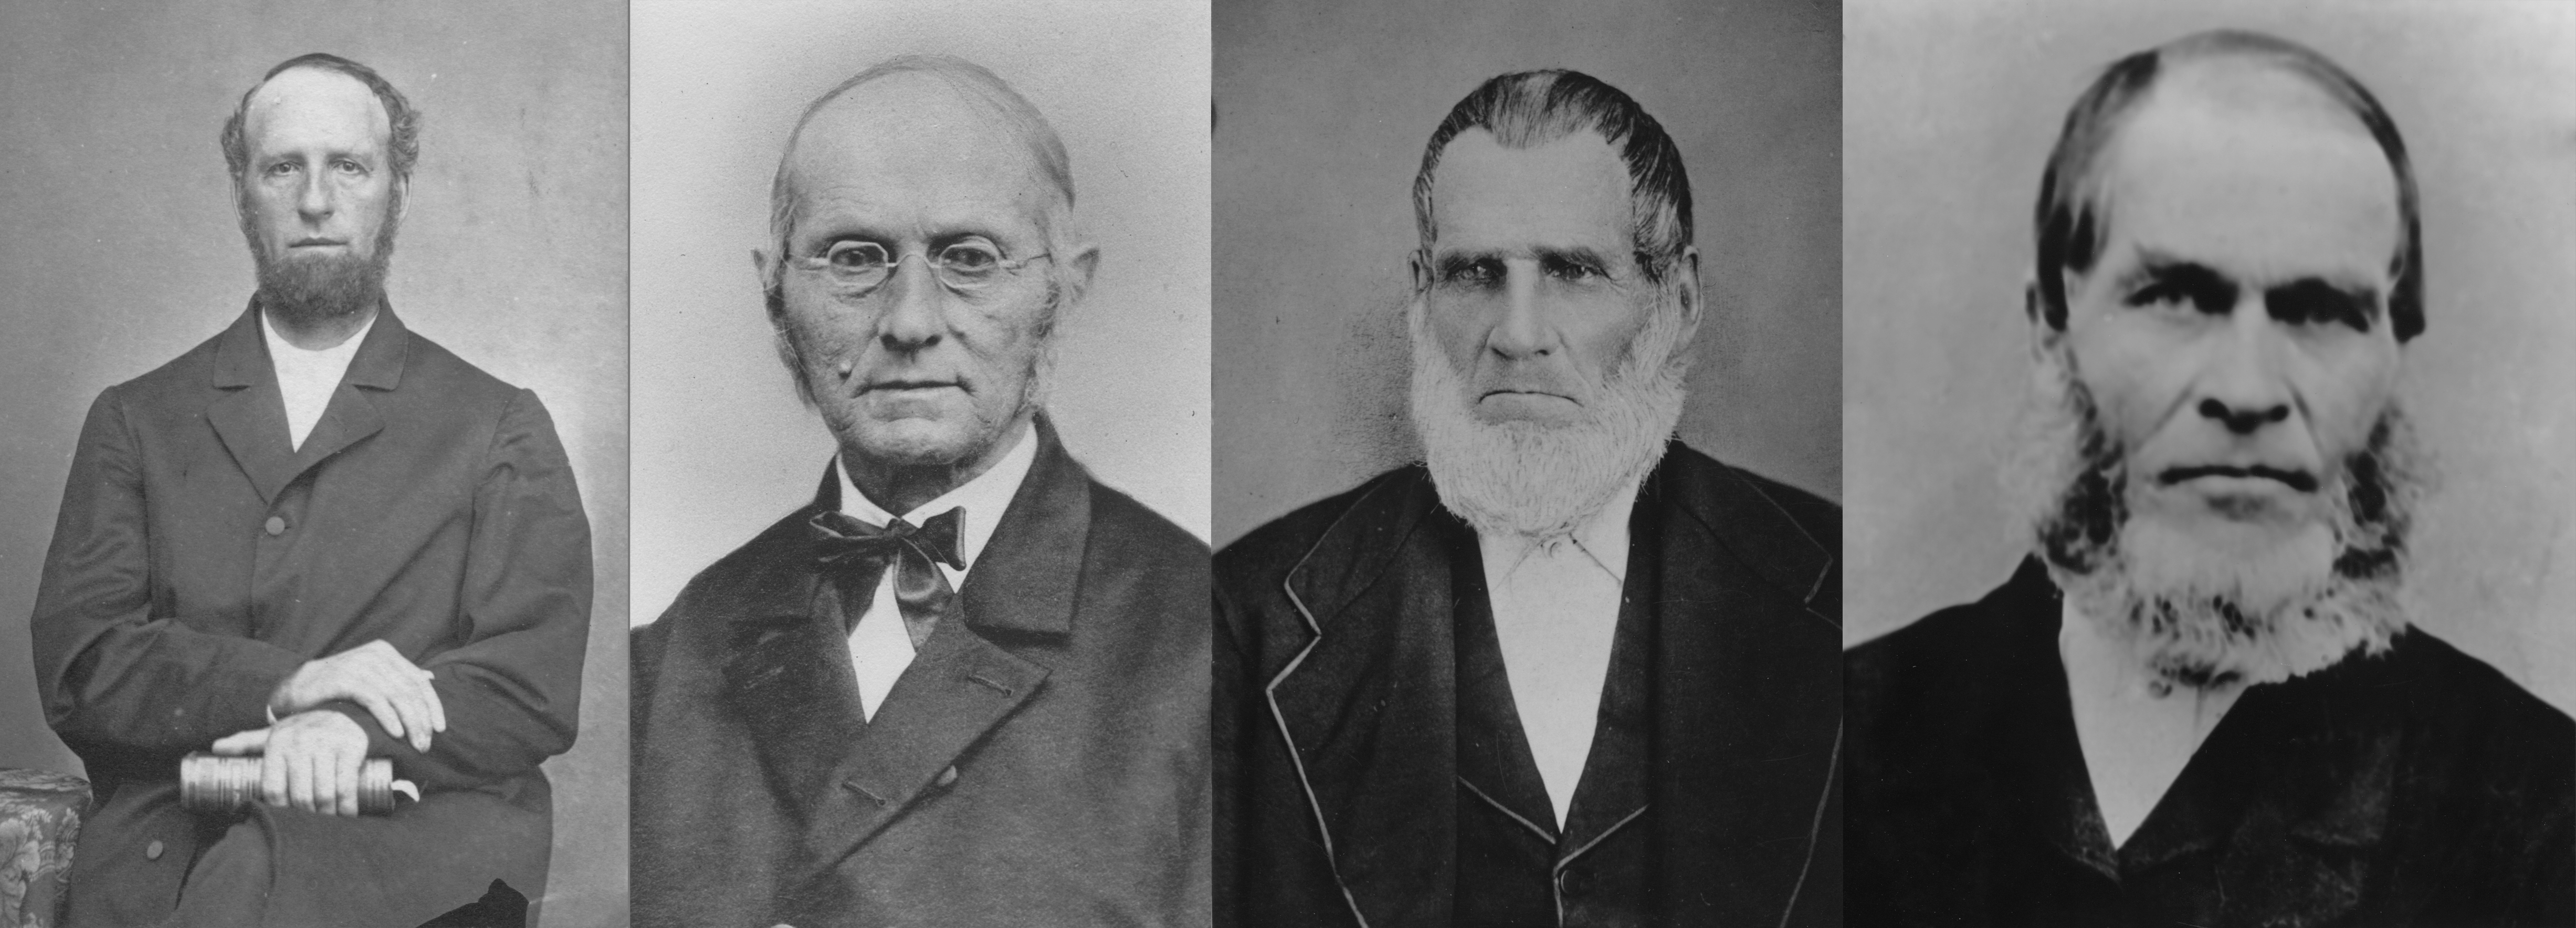
\includegraphics[width=1\linewidth]{images/james-white-joseph-bates-stephen-pierce-hiram-edson.jpg}
    \caption*{James White, Joseph Bates, Stephen Pierce, Hiram Edson}
    \label{fig:pioneers}
\end{figure}

\egwnogap{Przez cały ten czas nie mogłam zrozumieć rozumowania braci. Mój umysł był jakby zablokowany i nie mogłam pojąć znaczenia studiowanych przez nas fragmentów Pisma Świętego. Był to jeden z największych smutków mojego życia. \textbf{Pozostawałam w tym stanie umysłu, dopóki wszystkie \underline{główne punkty naszej wiary} nie zostały wyjaśnione w naszych umysłach, w harmonii ze Słowem Bożym}. Bracia wiedzieli, że gdy nie byłam w widzeniu, nie mogłam zrozumieć tych spraw, i przyjmowali objawienia jako światło bezpośrednio z nieba}[SpTB02 57.1; 1904][https://egwwritings.org/read?panels=p417.291]

\egwnogap{Przez dwa lub trzy lata mój umysł pozostawał zamknięty na zrozumienie Pisma Świętego. W trakcie naszej pracy, mój mąż i ja odwiedziliśmy ojca Andrews, który cierpiał na silny reumatyzm zapalny. Modliliśmy się za niego. Położyłam ręce na jego głowie i powiedziałam: «Ojcze Andrews, Pan Jezus cię uzdrawia». Został uzdrowiony natychmiast. Wstał i chodził po pokoju, chwaląc Boga i mówiąc: «Nigdy wcześniej nie widziałem czegoś takiego. Aniołowie Boży są w tym pokoju». Chwała Pańska została objawiona. Światło zdawało się świecić w całym domu, a ręka anioła została położona na mojej głowie. Od tamtego czasu aż do teraz jestem w stanie rozumieć Słowo Boże}[SpTB02 57.2; 1904][https://egwwritings.org/read?panels=p417.292]

\egwnogap{\textbf{Jaki wpływ skłania ludzi na tym etapie naszej historii do działania w podstępny, potężny sposób, aby \underline{zburzyć fundament naszej wiary} — fundament, który został położony na początku naszej pracy poprzez pełne modlitwy studium Słowa i przez objawienie? Na \underline{tym fundamencie} budujemy przez \underline{ostatnie pięćdziesiąt lat}. Czy dziwicie się, że gdy widzę początek działalności, która \underline{dąży do usunięcia niektórych z filarów naszej wiary}, mam coś do powiedzenia? Muszę być posłuszna rozkazowi: «Przeciwstaw się temu!»}}[SpTB02 58.1; 1904][https://egwwritings.org/read?panels=p417.295]

\egwnogap{Żywię najczulsze uczucia wobec dr. Kellogga. Przez wiele lat starałam się za nim obstawać. Słowo Boże zawsze mówiło mi: «Możesz mu pomóc». Czasami budzę się w nocy i chodząc po pokoju, modlę się: «O Panie, trzymaj dr. Kellogga mocno. Nie pozwól mu odejść. Zachowaj go niezłomnym. Namaść jego oczy niebiańską maścią, aby mógł widzieć wszystko wyraźnie». Noc po nocy leżałam bezsennie, zastanawiając się, jak mogę mu pomóc. Gorliwie i często modliłam się, aby Pan nie pozwolił mu odwrócić się od uświęcającej prawdy. To jest ciężar, który mnie przygniata — pragnienie, aby nie popełniał błędów, które zraniłyby jego duszę i \textbf{zaszkodziły sprawie teraźniejszej prawdy}. Ale od pewnego czasu jego działania ujawniają, że kieruje nim dziwny duch. Pan weźmie tę sprawę w swoje ręce. Muszę nieść poselstwa ostrzeżenia, które Bóg mi daje, a następnie pozostawić Panu rezultaty. \textbf{Muszę teraz przedstawić tę sprawę we wszystkich jej aspektach, ponieważ lud Boży nie może zostać splądrowany}}[SpTB02 58.2; 1904][https://egwwritings.org/read?panels=p417.296]

\egwnogap{\textbf{Jesteśmy zachowującym przykazania ludem Bożym. Przez ostatnie pięćdziesiąt lat była kierowana przeciwko nam każda forma herezji, aby zaciemnić nasze umysły w odniesieniu do nauczania Słowa} — \textbf{szczególnie odnośnie do służby Chrystusa w niebiańskiej świątyni i poselstwa niebios na te ostatnie dni, danego przez aniołów z czternastego rozdziału Księgi Objawienia}. \textbf{Poselstwa wszelkiego rodzaju i typu były narzucane Adwentystom Dnia Siódmego, aby zastąpić prawdę, która \underline{punkt po punkcie} została odkryta przez pełne modlitwy studium i potwierdzona przez cudotwórczą moc Pana}. \textbf{Lecz \underline{drogowskazy}, które \underline{uczyniły nas tym, czym jesteśmy}, \underline{mają być zachowane} i \underline{będą zachowane}, jak Bóg oznajmił przez swoje słowo i świadectwo swojego Ducha}. \textbf{Wzywa nas, abyśmy \underline{trzymali się mocno}, z uściskiem wiary, \underline{fundamentalnych zasad}, które są \underline{oparte na niepodważalnym autorytecie}}}[SpTB02 59.1; 1904][https://egwwritings.org/read?panels=p417.299]

Istniała konieczność ostrzeżenia Kościoła przed działaniem wroga zmierzającym do wykorzenienia fundamentu naszej wiary. Istniała konieczność przypomnienia Kościołowi, co stanowi prawdziwy fundament wiary Adwentystów Dnia Siódmego. Wydaje się, że Adwentyści Dnia Siódmego w tamtym czasie zapominali drogi, którą  \egwinline{Pan nas prowadził, oraz Jego nauk w naszej dotychczasowej historii}[LS 196.2; 1915][https://egwwritings.org/read?panels=p41.1083].

\egw{Jaki wpływ skłania ludzi na tym etapie naszej historii do działania w podstępny, potężny sposób, aby \textbf{zburzyć fundament naszej wiary} - fundament, który został położony \textbf{na początku naszego dzieła} poprzez pełne modlitwy studium Słowa i przez objawienie? Na \textbf{tym fundamencie} budujemy przez \textbf{ostatnie pięćdziesiąt lat}. Czy dziwicie się, że gdy widzę początek działalności, która \textbf{dąży do usunięcia niektórych z filarów naszej wiary}, mam coś do powiedzenia? Muszę być posłuszna rozkazowi: «\textbf{Przeciwstaw się temu}!»}[SpTB02 58.1; 1904][https://egwwritings.org/read?panels=p417.295]

Czemu siostra White zgodnie z tym poleceniem miała się przeciwstawić?

\egwinline{Mniej więcej w czasie, gdy opublikowano «The Living Temple»}, w porze nocnej zobaczyła ona \egwinline{obrazy wskazujące, że zbliża się jakieś niebezpieczeństwo}, i że musi się na nie \egwinline{przygotować poprzez spisanie rzeczy, które Bóg jej objawił} \egwinline{\textbf{odnośnie do fundamentalnych zasad naszej wiary}.}

Została \egwinline{pouczona przez niebiańskiego posłańca, że część rozumowania w książce «The Living Temple» jest niepoprawna i że \textbf{to rozumowanie sprowadziłoby na manowce} umysły tych, którzy nie są całkowicie utwierdzeni w \textbf{fundamentalnych zasadach} teraźniejszej prawdy.}

Więc jaki był faktyczny problem z książką \textit{The Living Temple}?

Jeśli jesteś uczonym, historykiem adwentystycznym, teologiem lub po prostu studentem teologii, zanim udzielisz prostej odpowiedzi i powiesz, że problemem był panteizm, chcielibyśmy zwrócić Twoją uwagę z powrotem na tekst. Siostra White jasno określiła istotę problemu, stwierdzając, że \textit{The Living Temple} \egwinline{wprowadza to, co jest niczym innym jak spekulacją w \textbf{odniesieniu do osobowości Boga i tego, gdzie jest Jego obecność}}.

Nie zaprzeczamy panteistycznemu problemowi książki, ale chcemy przekierować uwagę z błędu Kellogga na światło, które dał Bóg. Istnieją dwa sposoby podejścia do kryzysu Kellogga. Jeden polega na zajęciu się panteizmem, a drugi na zajęciu się \egwinline{\textbf{osobowością Boga} i \textbf{tym, gdzie jest Jego obecność}}. Jeden sposób to badanie błędu, a drugi to badanie Prawdy. Jeden sposób to analizowanie ciemności, a drugi to picie ze źródła Prawdy. Wybieramy to drugie i z tego powodu ta książka różni się od setek innych książek napisanych o kryzysie Kellogga. Tematem tej książki nie jest panteizm ani żaden inny błąd, ale prawda i to, co Bóg objawił o swojej osobowości i tym, gdzie jest Jego obecność. To był prawdziwy problem publikacji Kellogga.

Wierzymy, że studiowanie i analizowanie błędu jest bardzo niebezpieczne, ponieważ błąd prowadzi do zwiedzenia. Problem ze zwiedzeniem polega na tym, że możemy być zwiedzeni, oczywiście nie wiedząc, że jesteśmy zwiedzeni! Mocno wierzymy, że Ellen White była prorokiem Boga i że otrzymywała Światło od Boga, \bible{który jest światłością i nie ma w Nim żadnej ciemności}[1J 1:5]. Dlatego nie oczekujemy, że siostra White wyjaśni błędy w książce \textit{The Living Temple}. Wielu przychodziło do niej, prosząc ją \egwinline{o wyjaśnienie stanowisk zajętych w «The Living Temple»}. Odpowiadała: \egwinline{Są one niewytłumaczalne}. Jej celem nie było analizowanie błędu, ale rzucenie światła Prawdy na \emcap{osobowość Boga} i to, gdzie jest Jego obecność. W ten sposób wskazywała na prawdy, na których Bóg założył Kościół Adwentystów Dnia Siódmego. Te prawdy stanowiły fundament naszej wiary. Te prawdy zostały nam dane w naszych wczesnych dniach. Przekierowując naszą uwagę z osobowości Boga na panteizm, tracimy okazję, by pamiętać \egwinline{\textbf{drogę, którą Pan nas prowadził}, i \textbf{Jego nauki} w naszej \textbf{dotychczasowej historii}}. W tym świetle wyrażamy nasze zaniepokojenie kryzysem Kellogga i jego panteistycznym podejściem, ponieważ \egwinline{ścieżka prawdy biegnie blisko ścieżki błędu i obie ścieżki mogą wydawać się być jedną}; rozwiązaniem jest bycie \egwinline{całkowicie utwierdzonym w \textbf{fundamentalnych zasadach} teraźniejszej prawdy}. W innych miejscach siostra White mocno ugruntowała tę zasadę.

\egw{Szatan wcale nie śpi; jest on w pełni rozbudzony i rozgrywa grę o życie dusz ludu Bożego. Przyjdzie do nich z wszelkiego rodzaju pochlebstwami, mając nadzieję doprowadzić ich do zboczenia z drogi wierności. \textbf{Pragnie odwrócić ich uwagę od prawdziwych kwestii ku fałszywym teoriom}}[Ms132-1903.42; 1904][https://egwwritings.org/read?panels=p9056.56]

Skupmy więc naszą uwagę na prawdziwym problemie, a nie na fałszywych teoriach.

% Fundament naszej wiary

\begin{titledpoem}
    \stanza{
        Prawda wieczna mocno stoi, \\
        Żaden wróg jej nie rozbroi. \\
        Pan swą siłą dzieło tchnie, \\
        Wiernych posłów wspiera swe.
    }

    \stanza{
        Na platformie prawdy trwajmy, \\
        Filarów wiary się trzymajmy. \\
        To fundament dany nam, \\
        Który przetrwa czasu plan.
    }

    \stanza{
        Wróg chce usunąć prawdy te, \\
        Fałszywe teorie szerząc swe. \\
        Lecz Bóg wzbudzi wiernych swych, \\
        By strzec zasad odwiecznych tych.
    }

    \stanza{
        O Bożej osobowości nie spekulujmy, \\
        Mistycyzmu się wystrzegajmy. \\
        Ścieżka prawdy blisko błędu biegnie, \\
        Tylko Duch Święty nas bezpiecznie wiedzie.
    }
\end{titledpoem}

% Staranuj górę lodową

\begin{titledpoem}
    \stanza{
        "Staranuj ją!" - rozkaz brzmi, \\
        Gdy góra lodowa przed nami tkwi. \\
        Bez wahania naprzód płyń, \\
        By rozbić zwodniczy cień.
    }

    \stanza{
        Fundament wiary solidny jest, \\
        Przez pięćdziesiąt lat przetrwał test. \\
        Przez studiowanie i modlitwy żar, \\
        Bóg dał nam prawdy wiecznej dar.
    }

    \stanza{
        Zasady, które Bóg nam dał, \\
        By każdy wiernie przy nich stał. \\
        Nie pozwól, by je zabrał wróg, \\
        Gdy burzy to, co zbudował Bóg.
    }

    \stanza{
        Trzymajmy się więc mocno dziś, \\
        Tego, co dane nam przez Pana jest. \\
        Niech prawda jasno świeci nam, \\
        Aż wejdziemy do niebios bram.
    }
\end{titledpoem}
           % Chapter 1
\qrchapter{https://forgottenpillar.com/rsc/pl-fp-chapter2}{Fundamentalne zasady}

Prawdziwym problemem, według rozdziału dziesiątego \textit{Special Testimonies}, jest odejście od fundamentu naszej wiary, który został ustanowiony na początku naszego dzieła.

\egw{\textbf{Ten fundament został zbudowany przez Mistrza} i \underline{przetrwa} burzę i nawałnicę. Czy pozwolą temu człowiekowi \textbf{przedstawiać doktryny, które zaprzeczają doświadczeniom z przeszłości} ludu Bożego? Nadszedł czas, aby podjąć zdecydowane działanie}[SpTB02 54.2; 1904][https://egwwritings.org/read?panels=p417.276]

Kellogg przedstawił doktryny, które zaprzeczają doświadczeniom z przeszłości. W innym miejscu napisała o Kelloggu:

\egw{Bardzo martwię się o dr. Kellogga. Pod wieloma względami jego postępowanie nie podoba się Panu. Wydaje się, że \textbf{tak łatwo jest mu odejść od \underline{fundamentalnych zasad}}. Jest w wielkim niebezpieczeństwie, że \textbf{nie zachowa swoich początkowych przekonań} aż do końca}[Lt138-1902.5; 1902][https://egwwritings.org/read?panels=p9219.11]

Problemem było odejście od fundamentalnych zasad — ale nie wszyscy ludzie to dostrzegli. Szczególnie kluczowi i znaczący ludzie w dziele zapomnieli drogi, którą Pan ich prowadził, oraz Jego nauk w przeszłości.

\egw{Miałam nadzieję, że nastąpi gruntowna reforma i że \textbf{zasady}, o które walczyliśmy \textbf{we wczesnych dniach} i które zostały wprowadzone w mocy Ducha Świętego, \textbf{będą zachowane}}[SpTB02 56.3; 1904][https://egwwritings.org/read?panels=p417.287]

Jakie były zasady, o które walczyliśmy we wczesnych dniach? Co było tym fundamentem naszej wiary?

\egw{Jako lud mamy \textbf{stać niewzruszenie na platformie wiecznej prawdy}, która przetrwała próby i doświadczenia. Mamy \textbf{trzymać się pewnych filarów naszej wiary}. \textbf{\underline{Zasady prawdy}}, które Bóg nam objawił, \textbf{są naszym jedynym prawdziwym fundamentem}. To one uczyniły nas tym, czym jesteśmy...}[SpTB02 51.2; 1904][https://egwwritings.org/read?panels=p417.261]

\egwinline{Zasady prawdy}, które Bóg objawił, \egwinline{są naszym jedynym prawdziwym fundamentem}. Nazywa ona te zasady platformą wiecznej prawdy. Odnosi się do tych zasad jako do \egwinline{pewnych filarów naszej wiary}[SpTB02 51.2; 1904][https://egwwritings.org/read?panels=p417.261].

Przypomina ona o wcześniejszych doświadczeniach naszych pionierów, takich jak James White, Joseph Bates, starszy Edson, ojciec Pierce, jak Bóg pracował nad nimi, aż \egwinline{punkt po punkcie} \egwinline{wszystkie \textbf{główne punkty naszej wiary} zostały wyjaśnione}. Przypomniała, jak \egwinline{ten fundament został zbudowany przez Mistrza} i zapewnia, że \egwinline{przetrwa burzę i nawałnicę}. Podsumowując, zdecydowanie potwierdziła wolę Boga wobec nas w odniesieniu do tych zasad. Bóg \egwinline{wzywa nas, abyśmy trzymali się mocno, z uściskiem wiary, \textbf{fundamentalnych zasad}, które są oparte na niepodważalnym autorytecie}.

Widzimy kilka różnych wyrażeń, których siostra White użyła w odniesieniu do fundamentu naszej wiary: „\textit{platforma wiecznej prawdy}”, „\textit{filary naszej wiary}”, „\textit{zasady prawdy}”, „\textit{główne punkty}”, „\textit{drogowskazy}” i „\textit{fundamentalne zasady}”. Wyrażenia te oznaczają to samo — \textit{fundament naszej wiary}. Kiedy dziś słyszymy te wyrażenia, jakoś nie przekazują one żadnych konkretnych informacji. Ale dla Adwentystów Dnia Siódmego w jej czasach było to bardzo jasne i konkretne. Wszystkie te terminy odnoszą się do publicznego streszczenia wiary Adwentystów Dnia Siódmego, zwanego \emcap{Fundamentalnymi Zasadami}, wyjaśnionymi poniżej.

Bóg \egwinline{wzywa nas, abyśmy \textbf{trzymali się mocno}, z uściskiem wiary, \textbf{\underline{fundamentalnych zasad}}, które \textbf{są oparte na niepodważalnym autorytecie}}. Jest to odniesienie do głównych aspektów wiary Adwentystów Dnia Siódmego, które Bóg objawił pionierom adwentyzmu \egwinline{po upływie czasu w 1844 roku}, gdy grupa gorliwych, szlachetnych i prawych mężczyzn \egwinline{poszukiwała prawdy jak ukrytego skarbu}. To był \textit{fundament naszej wiary}. Nasi pionierzy oficjalnie założyli Kościół Adwentystów Dnia Siódmego w 1863 roku i nauczali tych prawd, które nazwali „\textit{fundamentalnymi zasadami}”. Jednak często Adwentyści Dnia Siódmego byli publicznie przedstawiani w niewłaściwy sposób. Z tego powodu w 1872 roku nasi pionierzy opublikowali dokument zatytułowany „\textit{Deklaracja Fundamentalnych Zasad, nauczanych i praktykowanych przez Adwentystów Dnia Siódmego}” w celu publicznego i zwięzłego zadeklarowania, jakich \emcap{fundamentalnych zasad} nauczali i przestrzegali Adwentyści Dnia Siódmego. Te \emcap{Fundamentalne Zasady} były regularnie drukowane jako osobna broszura, były obecne w naszych czasopismach i były corocznie drukowane w Rocznikach Adwentystycznych przez całe życie Ellen White.\footnote{Zobacz \hyperref[appendix:timeline]{Fundamentalne Zasady — Oś czasu}, aby uzyskać więcej szczegółów.} Dlatego gdy Ellen White odnosiła się do „\textit{fundamentalnych zasad}”, nie było to mgliste czy niejasne stwierdzenie, ponieważ Kościół Adwentystów Dnia Siódmego oficjalnie i publicznie zadeklarował, czym były te \emcap{fundamentalne zasady}. We wstępie do tego dokumentu czytamy o celu, który temu dokumentowi przyświecał.

\begin{figure}
    \centering
    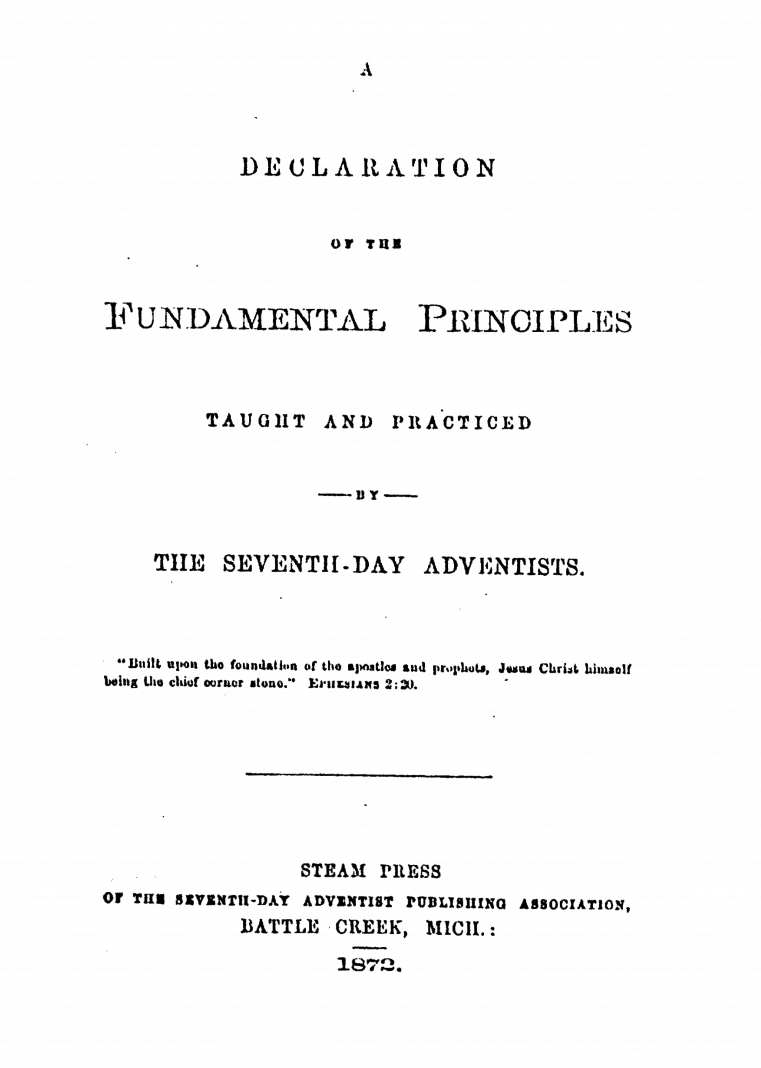
\includegraphics[width=1\linewidth]{images/declaration-of-the-fundamental-principles.PNG}
    \caption*{Skan Deklaracji Fundamentalnych Zasad, 1872.}
    \label{fig:declaration-of-the-fundamental-principles}
\end{figure}

\others{Przedstawiając \textbf{publicznie} to \textbf{streszczenie naszej wiary}, pragniemy, aby wyraźnie zrozumiano, że \textbf{nie mamy żadnych artykułów wiary, wyznania wiary ani dyscypliny} \textbf{\underline{poza Biblią}}. \textbf{Nie} przedstawiamy tego \textbf{jako coś, co ma jakikolwiek autorytet wśród naszych ludzi}, \textbf{ani nie ma to na celu zapewnienia jednolitości wśród nich}, \textbf{jako system wiary}, \textbf{ale jest to krótkie oświadczenie tego, }\textbf{\underline{co jest i było, z wielką jednomyślnością, wyznawane przez nich}}. Często jest konieczne, aby odpowiadać na pytania dotyczące tego tematu, a czasami korygować fałszywe stwierdzenia rozpowszechniane przeciwko nam i usuwać błędne wrażenia, które powstały u tych, którzy nie mieli okazji zapoznać się z naszą wiarą i praktyką. Naszym jedynym celem jest sprostanie tej potrzebie}

\others{\textbf{Jako Adwentyści Dnia Siódmego pragniemy jedynie, aby nasze stanowisko było zrozumiane}; tym bardziej nam na tym zależy, ponieważ jest wielu, którzy nazywają siebie adwentystami, a głoszą poglądy, z którymi nie możemy się zgodzić, z których niektóre, jak sądzimy, podważają najprostsze i najważniejsze zasady przedstawione w Słowie Bożym...}[The Fundamental Principles 1872, str. 3.1][https://egwwritings.org/read?panels=p928.8]

To streszczenie wiary składało się z 25 punktów, które reprezentowały to, co \othersnodot{jest i było, z wielką jednomyślnością, wyznawane przez} Adwentystów Dnia Siódmego. Te 25 punktów stanowiło \egwinline{\textbf{fundament}, który został \textbf{położony na początku} naszego dzieła \textbf{poprzez pełne modlitwy studium} Słowa i przez objawienie}. W 1904 roku siostra White powiedziała nam, że \egwinline{na \textbf{tym fundamencie} budujemy przez \textbf{ostatnie pięćdziesiąt lat}}. To są \egwinline{\textbf{fundamentalne zasady, które są oparte na niepodważalnym autorytecie}}, których Bóg \egwinline{wzywa nas, abyśmy \textbf{trzymali się mocno}, z uściskiem wiary}. Innymi słowy, powtórzyła, że \egwinline{mamy \textbf{trzymać się pewnych filarów naszej wiary}}.

W 1904 roku siostra White pisała o \egwinline{\textbf{staraniach wroga, aby podkopać fundament naszej wiary}}. Pisała o ruchu, który miałby \egwinline{polegać na \textbf{porzuceniu} doktryn, które stoją jako \textbf{filary naszej wiary}}. Ta reforma, gdyby została przyjęta, odrzuciłaby \egwinline{\textbf{zasady prawdy}, które Bóg w swojej mądrości dał Kościołowi ostatków}, i \egwinline{\textbf{fundamentalne zasady}, które podtrzymywały dzieło przez ostatnie pięćdziesiąt lat, \textbf{zostałyby uznane za błąd}}. Ruch ten rozpoczął się mniej więcej w czasie, gdy dr John H. Kellogg opublikował książkę \textit{The Living Temple}\footnote{Pl. \textit{Żyjąca Świątynia} (przyp. tłum.).}.

\egw{Mniej więcej w czasie, gdy opublikowano «The Living Temple», w porze nocnej przeszły przede mną \textbf{obrazy wskazujące, że zbliża się jakieś niebezpieczeństwo}, i że muszę się na nie przygotować poprzez  \textbf{spisanie rzeczy}, które Bóg mi objawił \textbf{odnośnie do \underline{fundamentalnych zasad naszej wiary}}}[SpTB02 52.3; 1904][https://egwwritings.org/read?panels=p417.267]

Przez opublikowanie książki \textit{The Living Temple} \textbf{fundamentalne zasady naszej wiary} \textbf{miały być podważone} \egwinline{poprzez rozpowszechnianie \textbf{zwodniczych teorii}} w niej zawartych.

\egw{Zostałam pouczona przez niebiańskiego posłańca, że część rozumowania w książce «The Living Temple» jest niepoprawna i że \textbf{to rozumowanie sprowadziłoby na manowce} umysły tych, którzy nie są całkowicie utwierdzeni w \textbf{fundamentalnych zasadach} teraźniejszej prawdy. Wprowadza to, co jest niczym innym jak spekulacją w \textbf{odniesieniu do \underline{osobowości Boga i tego, gdzie jest Jego obecność}}}[SpTB02 51.3; 1904][https://egwwritings.org/read?panels=p417.262]

Siostra White zwraca szczególną uwagę na to, że rozumowanie zawarte w książce \textit{The Living Temple} \egwinline{\textbf{sprowadziłoby na manowce}} z \egwinline{\textbf{fundamentalnych zasad} teraźniejszej prawdy}. To rozumowanie dotyczy \egwinline{\textbf{osobowości Boga i tego, gdzie jest Jego obecność}}.

Jak wspomniano wcześniej, słowo ‘\textit{osobowość}’ w kontekście dziewiętnastego wieku jest definiowane jako „\textit{właściwość lub stan bycia osobą}”\footnote{\href{https://www.merriam-webster.com/dictionary/personality}{Merriam-Webster Dictionary}, słowo ‘\textit{personality}’.}. Innymi słowy, termin ten odpowiada na pytania: „\textit{Co definiuje kogoś jako osobę?}”, „\textit{Jaka jest właściwość lub stan kogoś jako osoby?}”. W przypadku \emcap{osobowości Boga} pytanie brzmi: „\textit{Czy Bóg jest osobą i co definiuje Go jako osobę? Jaka jest właściwość lub stan Boga jako osoby?}”.

Rozumowanie dr. Kellogga dotyczące tych kwestii, wyrażone w książce \textit{The Living Temple}, jest \egwinline{niepoprawne}. Poglądy dotyczące \egwinline{\textbf{osobowości Boga i tego, gdzie jest Jego obecność}}, \egwinline{propagowane w książce, nie miały poparcia Boga i były \textbf{sidłem, które wróg przygotował na ostatnie dni}}. Ponieważ żyjemy w czasach końca, powinniśmy zadać sobie te pytania. Powinniśmy również badać biblijną ważność stwierdzeń w \emcap{Fundamentalnych Zasadach} dotyczących \emcap{osobowości Boga} i tego, gdzie jest Jego obecność. Jak \emcap{Fundamentalne Zasady} definiują Boga jako osobę i co mówią w odniesieniu do Bożej obecności?

Pierwszy punkt wymieniony poniżej dotyczy \emcap{osobowości Boga} i Jego obecności. Drugi punkt daje kontekst pierwszemu. Prosimy o rozważenie kilku pytań podczas ich czytania: Kto jest określany jako jeden Bóg? Jak Bóg jest definiowany jako osoba albo, innymi słowy, jaka jest Jego właściwość lub stan jako osoby? W jaki sposób te punkty mówią o obecności Boga?

\others{I — Że jest \textbf{jeden Bóg}, \textbf{\underline{osobowa, duchowa istota}}, \textbf{stwórca wszystkich rzeczy}, wszechmocny, wszechwiedzący i wieczny, nieskończony w mądrości, świętości, sprawiedliwości, dobroci, prawdzie i miłosierdziu; niezmienny i \textbf{\underline{wszędzie obecny przez swego przedstawiciela, Ducha Świętego}}. Ps 139:7}

\othersnogap{II — Że jest \textbf{jeden Pan Jezus Chrystus}, \textbf{\underline{Syn Wiecznego Ojca}}, ten, \textbf{\underline{przez}}\textbf{ którego Bóg stworzył wszystkie rzeczy} i przez którego one istnieją...}[Fundamentalne Zasady (1889), punkt nr 1 i 2.] \footnote{Pełna lista Fundamentalnych Zasad znajduje się w \hyperref[chap:appendix]{Dodatku}.} \footnote{Od 1872 do 1914 roku Fundamentalne Zasady pozostawały stałe i niezmienione, z wyjątkiem 1889 roku, kiedy James Smith dodał trzy nowe punkty. Jednak przez wszystkie te lata punkty dotyczące \textit{„osobowości Boga”} i \textit{„tego, gdzie jest Jego obecność”}, pozostawały bez zmian.}

W czasach Ellen White Adwentyści Dnia Siódmego wierzyli w jednego Boga — osobową, duchową istotę, Stwórcę wszystkich rzeczy — i wierzyli, że ten Bóg stworzył wszystko przez swojego Syna Jezusa Chrystusa. Zwracali się do Ojca jako jedynego Boga, a do Chrystusa jako Syna Bożego. Właściwość lub stan Boga jako osoby wyrażono w określeniu „\textit{osobowa, duchowa istota}”. Co do Jego obecności, \emcap{Fundamentalne Zasady} stwierdzają, że jest On wszędzie obecny przez swojego przedstawiciela, Ducha Świętego. Znaczenie tych zasad wymaga szczególnej uwagi. W obrębie kontekstu historycznego będzie to przedmiotem naszych dalszych badań.

\section*{Próba}

Najbardziej oczywiste jest to, że te \emcap{fundamentalne zasady} nie zawierają doktryny o Trójcy! Dokładniej mówiąc, wyrażenia: „\textit{trzech w jednym}” lub „\textit{jeden w trzech}”, w odniesieniu do Boga, nie występują nigdzie — choć są obecne w dzisiejszych \textit{Zasadach Wiary}. Tylko Ojciec jest określany jako „\textit{jeden Bóg}”. Lecz zanim wyciągniemy pochopne wnioski i potępimy doktrynę o Trójcy jako \egwinline{\textbf{zwodnicze teorie}}, które \egwinline{\textbf{podkopują fundament naszej wiary}}, należy pamiętać, że siostra White przedstawia wyczerpującą listę charakterystyk, które muszą być spełnione, aby doktryna o Trójcy została za taką teorię uznana.

Jeśli doktryna Trójcy jest wątpliwa, to trynitarne poglądy musiałyby:
\begin{itemize}
    \item okradać lud Boży z jego doświadczeń w przeszłości,
    \item niszczyć \emcap{osobowość Boga},
    \item burzyć filary naszej wiary lub sprowadzać na manowce z fundamentalnych zasad,
    \item być przedstawiane tak, jakby pani White je popierała.
\end{itemize}

Nie jest naszym zamiarem zajmować się którąkolwiek ze zwodniczych teorii Kellogga, ale raczej przestudiować \emcap{osobowość Boga} w jej historycznym kontekście. Czyniąc to, napotkamy dowody na to, że siostra White reagowała, ostrzegając Kościół przed tymi charakterystykami.

\begin{titledpoem}
    \stanza{
        Mistrz wybudował solidne podstawy, \\
        By wieść lud Boży w czasie tej długiej przeprawy. \\
        Te prawdy otrzymane w modlitwie i znoju \\
        Na bezsprzecznym gruncie prosto z nieba stoją.
    }

    \stanza{
        Bóg — jedna osobowa istota duchowa; \\
        Przed Jego Duchem i wzrokiem nic się tu nie schowa. \\
        Chrystus — to Syn Ojca Przedwiecznego; \\
        Trzymajmy się filara wiary tak pewnego.
    }

    \stanza{
        Gdy człowiek odchodzi od zasad prawdziwych, \\
        Burząc fundamenty na rzecz nauk fałszywych, \\
        Wówczas mądrość wieków tak szybko odrzuca, \\
        A schodząc z dobrej ścieżki, i Boga zasmuca.
    }

    \stanza{
        Trzymajmy się prawdy — mocno, niezachwianie; \\
        Niech z kotwicą wiary nikt się nie rozstanie. \\
        Bo co Bóg położył przez pionierów dłonie, \\
        Po burzy pozostanie już na nieboskłonie.
    }
\end{titledpoem}

           % Chapter 2
\chapter{ Kontekst Historyczny}

Ellen White wspomniała, że napotkała te same poglądy w \textit{The Living Temple}, przed którymi ostrzegała na początku swojej służby:

\egw{Gdy czytaliśmy \normaltext{[The Living Temple]}, rozpoznałam te same poglądy, przeciwko którym zostałam wezwana do ostrzeżenia \textbf{podczas wczesnych dni mojej publicznej służby}. \textbf{Gdy po raz pierwszy opuściłam \underline{stan Maine, było to po to, by udać się przez Vermont i Massachusetts}}, aby nieść świadectwo \textbf{przeciwko tym poglądom}. ‘Living Temple’ zawiera alfę tych teorii. Wiedziałam, że omega nastąpi wkrótce; i drżałam o nasz lud. Wiedziałam, że muszę ostrzec naszych braci i siostry, \textbf{aby nie wdawali się w spory dotyczące \underline{obecności i osobowości Boga}}. Stwierdzenia zawarte w ‘Living Temple’ odnośnie tej kwestii są nieprawidłowe. Pismo Święte użyte do poparcia przedstawionej tam doktryny jest błędnie zastosowane.}[SpTB02 53.2; 1904][https://egwwritings.org/?ref=en\_SpTB02.53.2&para=417.271]

Wskazała swoje pierwsze spotkanie z tymi poglądami: \egw{Gdy po raz pierwszy opuściłam \textbf{stan Maine}, było to po to, by udać się przez Vermont i Massachusetts, \textbf{aby nieść świadectwo przeciwko tym poglądom.}} Jej biografia, napisana przez jej wnuka Arthura Lacey White'a, dostarcza szerszego kontekstu dotyczącego tych poglądów. W książce \textit{Ellen White: The Early Years}, w sekcji \textit{Wrestling with the Views of the Spiritualizers}, jej doświadczenia we wschodnim Maine ujawniają więcej na temat kontrowersji dotyczącej osobowości Boga i jej następstwa.

\othersQuote{\textbf{\underline{We wschodnim Maine Ellen podróżowała}} i pracowała \textbf{w atmosferze spirytualistów, którzy \underline{alegorycznie znieśli niebo, Boga, Jezusa i nadzieję Adwentu}}. W wizji w Exeter w połowie lutego wydawało się, że \textbf{znajduje się w obecności Jezusa i gorliwie pragnęła uzyskać odpowiedzi na niektóre \underline{istotne pytania}}.}[ALW, 1BIO 79.4; 1985][https://egwwritings.org/?ref=en\_1BIO.79.4&para=668.582]

\othersQuoteNoGap{Zapytałam Jezusa, czy \textbf{Jego Ojciec ma postać podobną do Niego}. \textbf{Powiedział, że ma}, ale nie mogłam jej ujrzeć, ponieważ, jak powiedział: ‘Gdybyś choć raz ujrzała chwałę \textbf{Jego osoby}, przestałabyś istnieć.’ —Wczesne pisma, 54.}[ALW, 1BIO 79.5; 1985][https://egwwritings.org/?ref=en\_1BIO.79.5&para=668.583]

\othersQuoteNoGap{Nie była to jedyna okazja, gdy Ellen rozmawiała z Jezusem i aniołem \textbf{o \underline{osobie Jezusa} i o tym, że \underline{Bóg jest osobową istotą}}. \textbf{\underline{Odpowiedzi w pełni ją przekonały, że spirytualiści są w głębokim błędzie}}.}[ALW, 1BIO 80.1; 1985][https://egwwritings.org/?ref=en\_1BIO.80.1&para=668.586]

Wizja, o której wspomniał Arthur Lacey White, znana jest jako \textit{wizja o osobowości Boga}, którą zbadamy później. Ta wizja potwierdza, że doktryna \emcap{o osobowości Boga} naucza, że Bóg Ojciec ma postać, tak jak Jezus. Odnosi się ona szczególnie do \others{\textbf{osoby Jezusa} i do tego, że \textbf{Bóg jest osobową istotą}.}

Rozważmy pierwszy punkt \emcap{Fundamentalnych Zasad}, który stwierdza, że Adwentyści Dnia Siódmego wierzą w \others{jednego Boga, \textbf{osobową, duchową istotę}.}[First point of the Fundamental Principles][https://forgotten-pillar.s3.us-east-2.amazonaws.com/A+declaration+of+the+fundamental+principles+taught+and+practiced+by+the+Seventh-day+Adventists++.pdf] To jasno pokazuje, że główną kwestią w doktrynie \emcap{osobowości Boga} jest zewnętrzna, cielesna postać Ojca. Ale dlaczego było to tak istotne i znaczące pytanie? Jakie były implikacje tego, że Bóg ma cielesną, osobową postać?

\othersQuote{Ale ponieważ pionierzy Kościoła Adwentystów Dnia Siódmego utrzymywali, że proroctwo wypełniło się 22 października 1844 roku, i że ważna praca rozpoczęła się w niebie w Miejscu Najświętszym niebiańskiej świątyni w tym czasie, a ponieważ adwentyści, którzy stali się \textbf{spirytualistami} zajęli stanowisko, że Chrystus wszedł do ich serc 22 października 1844 roku, i że Jego królestwo jest w ich sercach, założyciele kościoła, a szczególnie Ellen White, byli klasyfikowani przez świat ogólnie, a także przez tych, których ADS określali jako adwentystów pierwszego dnia, jako jedna i ta sama grupa. Tu znowu wielki wróg rzucił oszczerstwo na prawdę, zestawiając ją z fałszywym, nieprawdziwym doświadczeniem.}[ALW, 1BIO 80.2; 1985][https://egwwritings.org/?ref=en\_1BIO.80.2&para=668.587]

\othersQuoteNoGap{Ellen White miała mówić o tej sprawie ponownie, szczególnie w końcowych akapitach swojej pierwszej małej książki, Experience and Views, opublikowanej w 1851 roku. Czytając to, należy zwrócić uwagę na użycie \textbf{terminu spirytualizm}, który musi być rozumiany w świetle działalności spirytualistów, a nie w świetle tego, co dziś rozumie się jako spirytualizm czy spirytyzm, chociaż oba pochodzą z tego samego źródła.}[ALW, 1BIO 80.3; 1985][https://egwwritings.org/?ref=en\_1BIO.80.3&para=668.588]

\othersQuoteNoGap{Przechodzimy teraz do oświadczenia napisanego i opublikowanego w 1851 roku, które znajduje się w Ibid., 77, 78:}[ALW, 1BIO 80.4; 1985][https://egwwritings.org/?ref=en\_1BIO.80.4&para=668.589]

\othersQuoteNoGap{\textbf{Często fałszywie oskarżano mnie o nauczanie poglądów charakterystycznych dla spirytualizmu}. Ale zanim redaktor The Day-Star popadł w to złudzenie, \textbf{Pan \underline{dał mi wizję} smutnych i niszczycielskich skutków, jakie on i inni wywołają w stadzie \underline{nauczając duchowych poglądów}}.}[ALW, 1BIO 80.5; 1985][https://egwwritings.org/?ref=en\_1BIO.80.5&para=668.590]

\othersQuoteNoGap{Często widziałam ukochanego \textbf{Jezusa, że jest On osobą}. Zapytałam Go \textbf{\underline{czy Jego Ojciec jest osobą} i \underline{ma postać} jak On}. Jezus odpowiedział: ‘Jestem \textbf{wyraźnym obrazem osoby Mojego Ojca}.}[ALW, 1BIO 80.6; 1985][https://egwwritings.org/?ref=en\_1BIO.80.6&para=668.591]

\othersQuoteNoGap{\textbf{Często widziałam, że \underline{duchowy pogląd} odebrał całą chwałę niebu, a w umysłach wielu ludzi tron Dawida i urocza osoba Jezusa zostały spalone w ogniu spirytualizmu.} Widziałam, że niektórzy, którzy zostali zwiedzeni i wprowadzeni w ten błąd, zostaną wyprowadzeni na światło prawdy, ale będzie prawie niemożliwe, aby całkowicie uwolnili się od \textbf{zwodniczej mocy spirytualizmu}. Tacy powinni dokładnie wyznać swoje błędy i na zawsze je porzucić.}[ALW, 1BIO 80.7; 1985][https://egwwritings.org/?ref=en\_1BIO.80.7&para=668.592]

\othersQuoteNoGap{\textbf{Uduchowienie nieba, Boga, Chrystusa i przyjścia Chrystusa leżało u podstaw wielu fanatycznych nauk, którym 17-letnia Ellen Harmon została powołana przez Boga, aby stawić czoła w tych formacyjnych dniach. Wizje stanowczo ustanowiły \underline{osobowość Boga i Chrystusa}, \underline{realność nieba} i nagrodę dla wiernych, oraz zmartwychwstanie. To rozsądne prowadzenie uratowało rodzący się kościół}.}[ALW, 1BIO 81.1; 1985][https://egwwritings.org/?ref=en\_1BIO.81.1&para=668.595]

Błąd ruchu Millerytów w 1844 roku polegał na niezrozumieniu natury wydarzenia, a nie jego czasu. Księga Daniela 7:13-14 opisuje Chrystusa przychodzącego do Sędziwego w niebie, aby otrzymać władzę, chwałę i królestwo - nie Jego drugie przyjście na ziemię. To wydarzenie, oznaczające początek pracy Chrystusa w Miejscu Najświętszym, nastąpiło na zakończenie proroctwa 2300 dni w 1844 roku. W przeciwieństwie do innych grup adwentystycznych, rodzący się Kościół Adwentystów Dnia Siódmego wyjątkowo rozpoznał to niebiańskie wydarzenie.

To zrozumienie opiera się na kluczowych założeniach:
\begin{itemize}
    \item Niebo jest realnym, dosłownym miejscem (Ew. Jana 14:1-3).
    \item W niebie istnieje dosłowna świątynia, w której służy Chrystus (Hebrajczyków 8:2).
    \item W tej świątyni istnieje realny, fizyczny tron, zajmowany przez samego Boga (Daniela 7:9-10; Objawienie 4:2-3; Ezechiela 1:26-28; Psalm 11:4).
\end{itemize}

Dlaczego kwestia cielesnej postaci Ojca jest tak ważna? Gdyby Bóg nie był istotą fizyczną, nie byłoby potrzeby dosłownego tronu, świątyni ani niebiańskiej służby. Uduchowiona interpretacja podważa fundament teologii Adwentystów Dnia Siódmego, prowadząc do efektu domina, który niszczy doktrynę o kapłańskiej służbie Chrystusa.

Doktryna o \emcap{osobowości Boga} była prostym, ale fundamentalnym nauczaniem, potwierdzonym w pierwszym punkcie \emcap{Fundamentalnych Zasad}: \textit{“Jeden Bóg, osobowa, duchowa istota.”} Jako taki, nie jest On wszechobecny sam w sobie, ale poprzez swojego przedstawiciela, Ducha Świętego.\footnote{Pierwszy punkt Fundamentalnych Zasad: \othersQuote{Że jest \textbf{jeden Bóg}, \textbf{\underline{osobowa, duchowa istota}}, stwórca wszystkich rzeczy, wszechmocny, ... i \textbf{wszędzie obecny przez \underline{swojego przedstawiciela}, Ducha Świętego}. Ps. 139:7.}} Kiedy Ellen White zapytała Jezusa \egwinline{czy Jego Ojciec \textbf{jest osobą} i \textbf{ma \underline{postać}} jak On,}[EW 77.1; 1882][https://egwwritings.org/read?panels=p28.490&index=0] widzimy wyraźnie, że \textit{zewnętrzna cielesna \textbf{postać}} jest \textit{cechą lub stanem} definiującym Boga jako osobę. To zrozumienie było kluczowe w rozwiązywaniu kryzysu Kellogga dotyczącego \textit{Żywej Świątyni}, która odbiegała od tego podstawowego przekonania.

Ale czy nasze obecne \textit{Fundamentalne Wierzenia} nadal potwierdzają tę doktrynę? Czy wyraźnie nauczają, że Bóg jest realną osobą o cielesnej postaci, której dosłowna obecność jest w niebie, podczas gdy jest On wszechobecny przez swojego Ducha? Doktryna o obecności i osobowości Boga jest nieobecna w dzisiejszych oficjalnych wierzeniach. Chociaż indywidualnie możemy nadal w to wierzyć, dlaczego tak istotne nauczanie zostało pominięte? Jakie były powody tej zmiany? To są pytania, które musimy dalej zgłębiać w kontekście \textit{Fundamentu Naszej Wiary}.

% The Historical Context
\begin{titledpoem}
    \stanza{
        Młoda Ellen przez Maine wędrowała, \\
        Przed błędnymi poglądami ostrzegała. \\
        Bóg ma postać, jak Chrystus objawił, \\
        I ten fakt w wizji Pan jej przedstawił.
    }

    \stanza{
        Spirytualista koncepcję swą sieje, \\
        Że fizyczne niebo wcale nie istnieje. \\
        Lecz osobowość Boga to nie abstrakcja pusta, \\
        To prawda, którą głosiły już pionierów usta.
    }

    \stanza{
        Alfa błędu w „Living Temple” się zjawiła, \\
        Omega wkrótce potem nastąpiła. \\
        Czy ta doktryna, niegdyś tak jasna, \\
        W naszych wierzeniach już nie wygasła?
    }
\end{titledpoem}
           % Chapter 3
\qrchapter{https://forgottenpillar.com/rsc/pl-fp-chapter4}{Korekta „The Living Temple”}

W \textit{Testimonies to the Church Containing Letters to Physicians and Ministers Instruction to Seventh-Day Adventists}, w rozdziale dziesiątym, „Fundament naszej wiary”, Bóg przekazał cenne lekcje na temat rozwoju i konsekwencji teorii Kellogga. Szersze i głębsze znaczenie tych cytatów można zrozumieć, gdy znamy ich historyczny kontekst. Przyjrzyjmy się najpierw pokrótce historycznemu kontekstowi książki Kellogga, \textit{The Living Temple}.

Poprzez szereg zrządzeń opatrzności Bóg dał do zrozumienia, że książka \textit{The Living Temple} nie powinna zostać wydrukowana. Jednym z takich wydarzeń było spalenie budynku drukarni w Battle Creek właśnie w noc przed planowanym drukiem. Ostatecznie jednak książka została wydrukowana gdzie indziej i wywołała wielki kryzys w Kościele Adwentystów Dnia Siódmego. 7 października 1903 roku w Waszyngtonie odbyło się doroczne spotkanie konferencji. Obecnych było wielu przywódców Kościoła Adwentystów Dnia Siódmego, w tym dr Kellogg i jego zwolennicy. Wokół tej książki toczył się poważny spór i konflikt był nieunikniony. Na szczęście w momencie narastającego konfliktu do rady dostarczono list od siostry White. W niedzielę list dotarł do uszu zgromadzonych, na co odpowiedziano wieloma „amen” i „alleluja”. Był to bardzo napięty i poruszający poranek dla Kościoła, który był na krawędzi rozłamu — by wreszcie otrzymać konkretne wskazówki od posłanniczki Pana:

\begin{figure}[h]
    \centering
    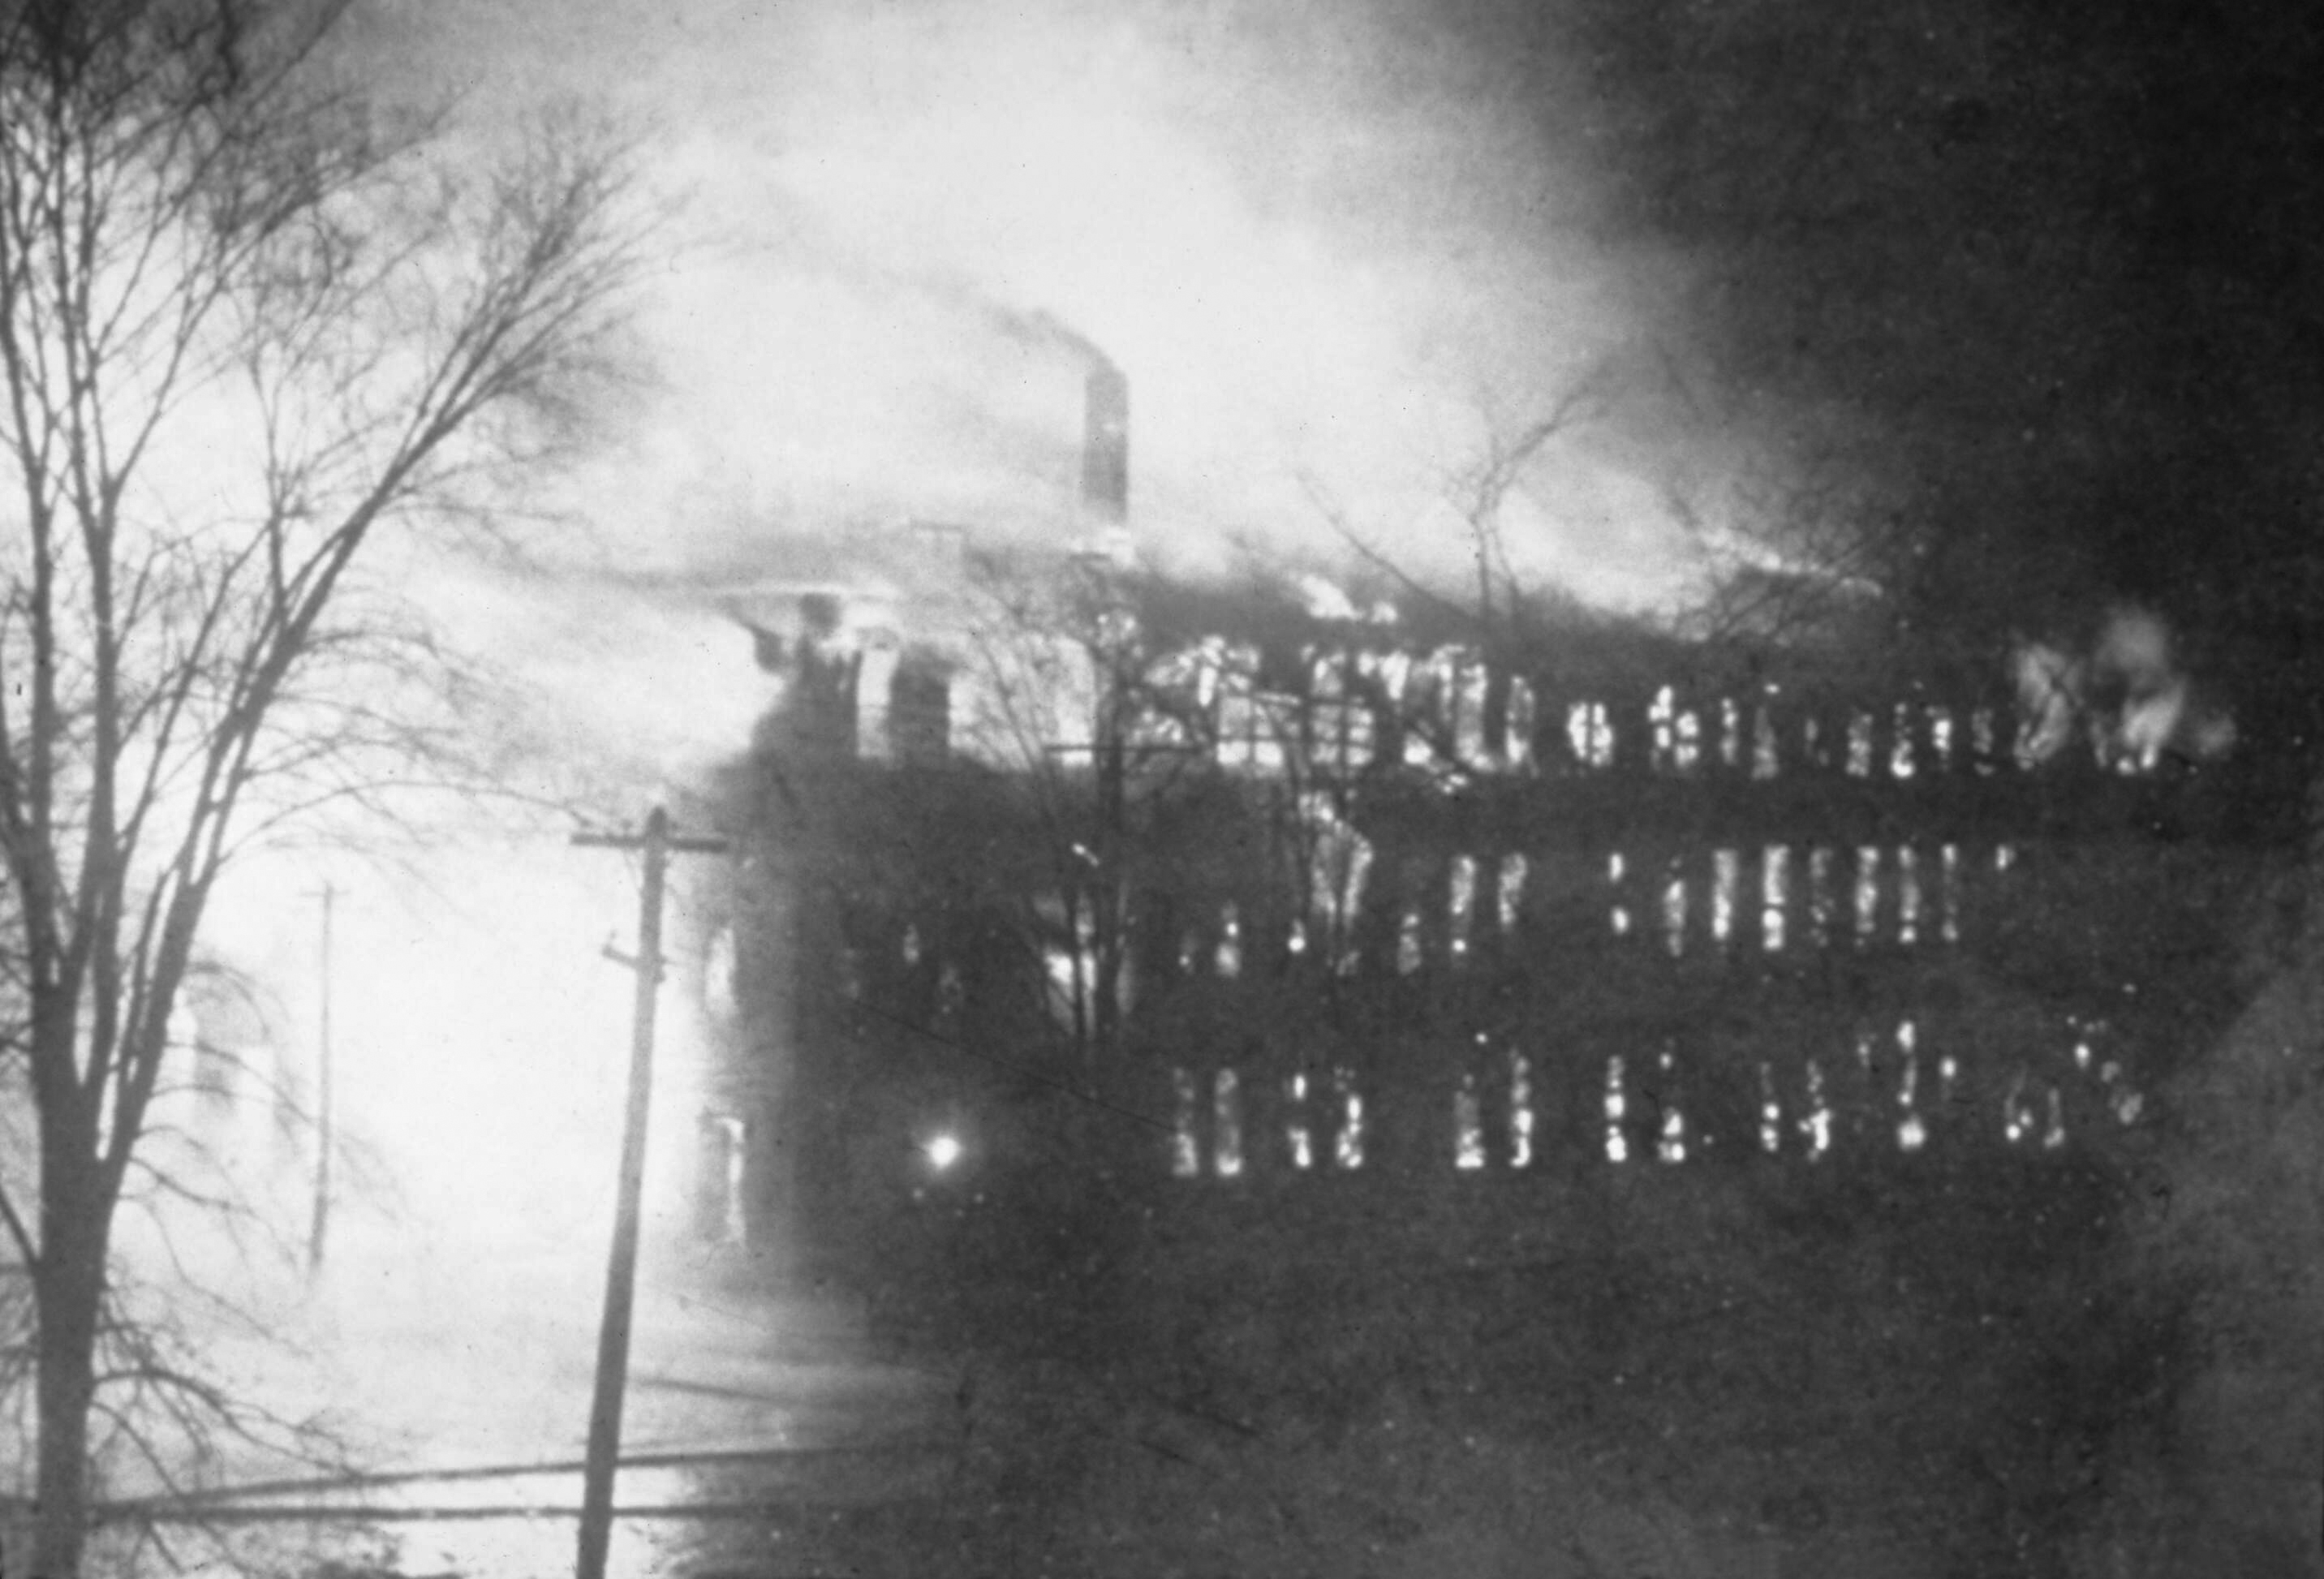
\includegraphics[width=1\linewidth]{images/review-and-herlad.jpg}
    \caption*{Spalenie budynku wydawnictwa Review and Herald, 30 grudnia 1902 r.}
    \label{fig:review-and-herald}
\end{figure}

\egw{Mam coś do powiedzenia naszym nauczycielom w odniesieniu do \textbf{nowej książki «The Living Temple»}. \textbf{Bądźcie ostrożni w popieraniu \underline{poglądów tej książki dotyczących osobowości Boga}}. Zgodnie z tym, jak Pan przedstawia mi te sprawy, \textbf{te poglądy nie mają poparcia Boga}. \textbf{Są one sidłem, które wróg przygotował na te ostatnie dni}. Myślałam, że zostanie to na pewno dostrzeżone i że nie będzie konieczne, abym cokolwiek o tym mówiła. \textbf{Ale ponieważ pojawia się twierdzenie, że nauki tej książki można poprzeć wypowiedziami z moich pism, jestem zmuszona zaprzeczyć temu twierdzeniu}. Mogą być w tej książce wyrażenia i poglądy, które są w zgodzie z moimi pismami. I mogą być w moich pismach liczne stwierdzenia, które wyrwane z kontekstu i interpretowane zgodnie z zamysłem autora «The Living Temple» wydawałyby się być zgodne z naukami tej książki. \textbf{Może to dawać pozorne poparcie twierdzeniu, że poglądy w «The Living Temple» są w zgodzie z moimi pismami}. \textbf{Ale broń Boże, żeby ta opinia przeważyła}}[Lt211-1903.1; 1903][https://egwwritings.org/?ref=en\_Lt211-1903.1]

Wielokrotnie siostra White stwierdzała, że prawdziwym problemem książki były poglądy \egwinline{\textbf{dotyczące osobowości Boga}}. Te poglądy nie są poparte stwierdzeniami z pism Ellen White i te właśnie poglądy \egwinline{\textbf{są pułapką, którą wróg przygotował na te ostatnie dni}}.

Bóg, ponownie w swojej opatrzności, rozwiązał ten konflikt. Kellogg przyjął naganę od posłanniczki Pana i przed zakończeniem rady oświadczył, że \textit{The Living Temple} zostanie wycofana z rynku\footnote{\href{https://forgottenpillar.com/wp-content/uploads/2022/04/Letter-A-G-Daniells-to-W-C-White-October-29-1903.pdf}{List: A. G. Daniells do W. C. White'a, 23 października 1903, str. 5}}. Jednak po konferencji rozmawiał prywatnie z przewodniczącym generalnej konferencji, bratem Arthurem G. Daniellsem, o swoich planach dotyczących książki. Poniżej przedstawiamy wybrane listy, ujawniające plany Kellogga dotyczące korekty \textit{The Living Temple}.

Ellen White nie była obecna na dorocznej konferencji w Waszyngtonie, ale jej syn, William C. White, w niej uczestniczył. Gdy konferencja się zakończyła, brat Arthur G. Daniells napisał poufny list do Williama C. White'a dotyczący planu dr Kellogga odnośnie do korekty jego książki:

\othersnodot{29 października 1903}

\othersnogap{Odkąd \textbf{rada została zamknięta}, czułem, że muszę napisać do Ciebie \textbf{poufnie w sprawie planów dr. Kellogga dotyczących korekty i publikacji «The Living Temple»} [...] On \normaltext{[Kellogg]} powiedział, że kilka dni przed przybyciem na radę, przemyślał tę sprawę i zaczął dostrzegać, że \textbf{popełnił niewielki błąd w wyrażaniu swoich poglądów}. Powiedział, że przez całą drogę był zatroskany o to, jak określić charakter Boga i jego związek z dziełami stworzenia...}

\begin{figure}[hp]
    \centering
    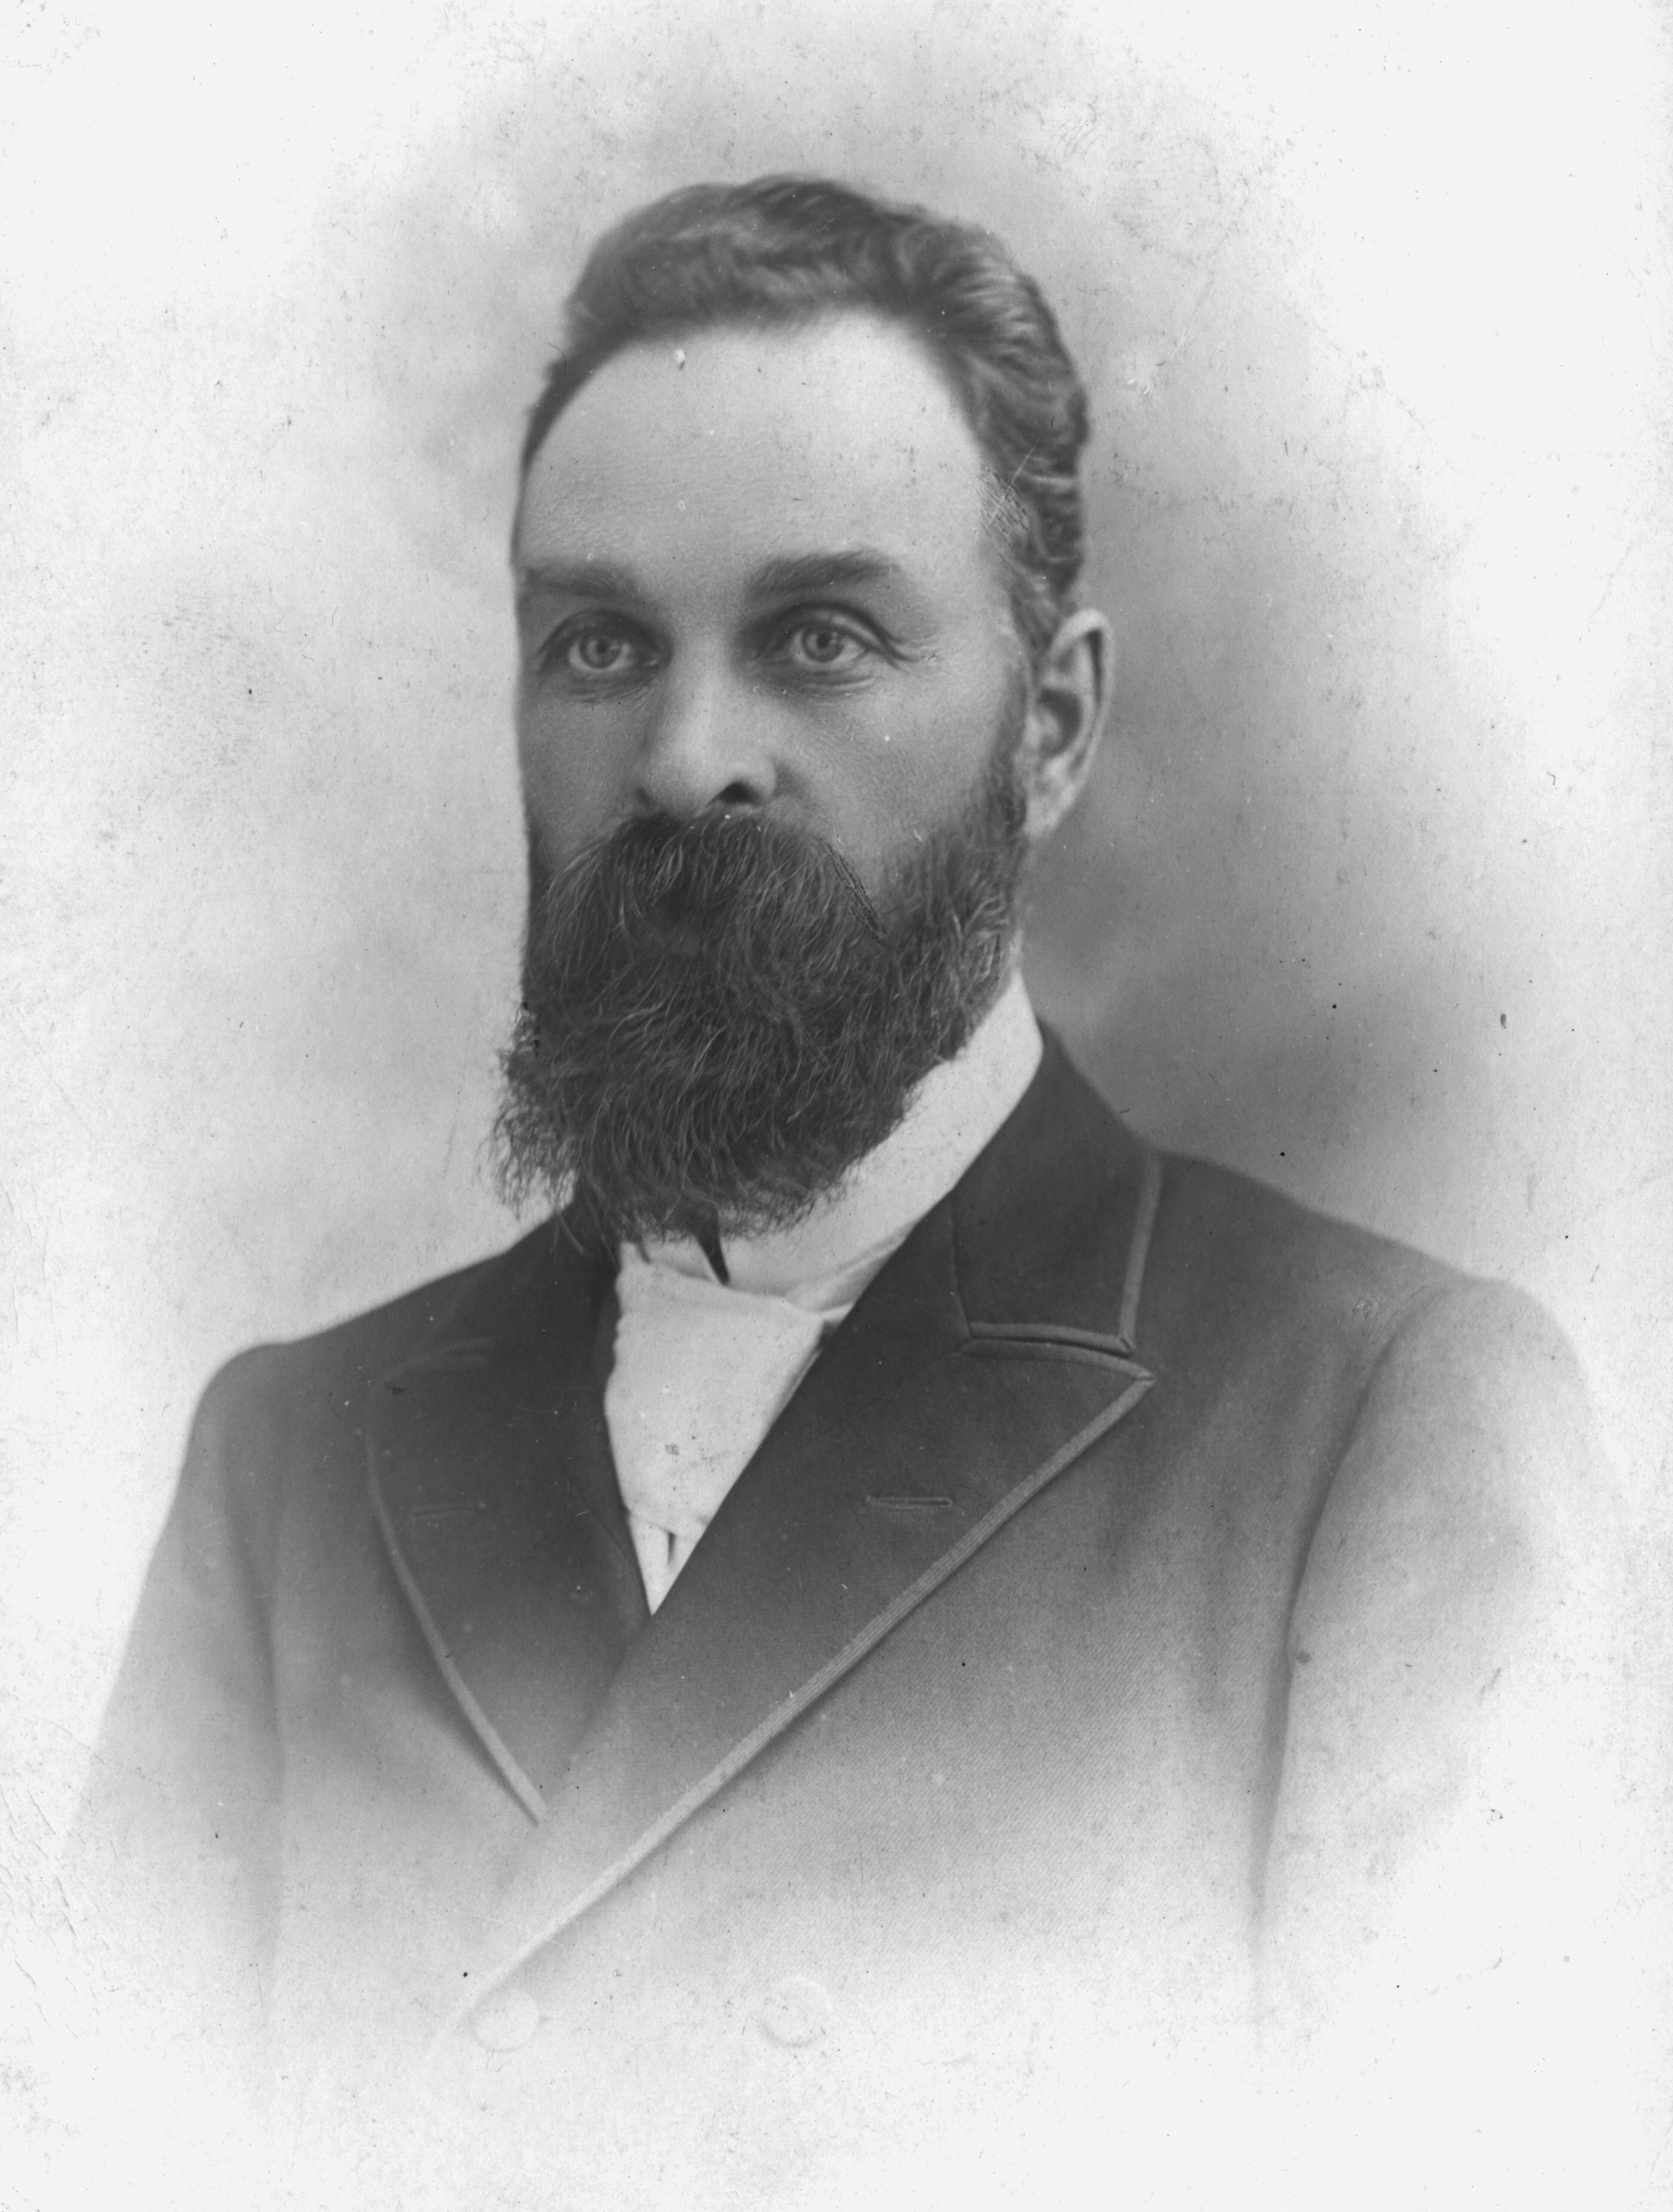
\includegraphics[width=1\linewidth]{images/daniels.jpg}
    \caption*{Arthur Grosvenor Daniells (1858-1935)}
    \label{fig:daniells}
\end{figure}

\othersnogap{\textbf{Następnie stwierdził, że jego wcześniejsze poglądy \underline{dotyczące trójcy} stanęły mu na drodze w złożeniu jasnego i całkowicie poprawnego oświadczenia; ale że niedługo potem \underline{zaczął wierzyć w trójcę} i mógł teraz całkiem wyraźnie zobaczyć, gdzie tkwił cały problem, i wierzył, że może wyjaśnić sprawę w satysfakcjonujący sposób}}

\othersnogap{\textbf{Powiedział mi, że teraz wierzy w \underline{Boga Ojca, Boga Syna i Boga Ducha Świętego}; a jego pogląd był taki, że to Bóg Duch Święty, a nie Bóg Ojciec, wypełnia całą przestrzeń i każdą żywą istotę. Powiedział, że gdyby  wierzył \underline{w to} przed napisaniem książki, to wyraziłby swoje poglądy bez wywoływania mylnego wrażenia, jakie teraz wywiera owa książka}}

\othersnogap{\textbf{Przedstawiłem mu zastrzeżenia, jakie znalazłem w tej nauce, i próbowałem mu pokazać, że nauka ta jest tak całkowicie sprzeczna z ewangelią, iż nie byłem w stanie sobie wyobrazić, jak można by ją poprawić, zmieniając tylko kilka wyrażeń}}

\othersnogap{Dyskutowaliśmy na ten temat dość długo w przyjaznej atmosferze; lecz byłem przekonany, że gdy się rozstaliśmy, doktor nie rozumiał ani siebie, ani charakteru swojego nauczania. Nie mogłem też pojąć, jak mógłby nagle zmienić zdanie i \textbf{w ciągu kilku dni \underline{poprawić książkę} tak, aby wszystko było w porządku}}[Letter: A. G. Daniells to W. C. White. October 29, 1903. pp. 1, 2][https://forgotten-pillar.s3.us-east-2.amazonaws.com/Letter-A-G-Daniells-to-W-C-White-October-29-1903.pdf]

Kellogg nie dostrzegał błędu w swoich poglądach, ale raczej w sposobie ich wyrażenia. Nie uważał, że jego poglądy były fałszywe, ale że sposób ich wyrażenia sprawił, iż książka dawała błędne wrażenie. Jednak najwyraźniej nie była to prawda. Jak stwierdziła siostra White, Kellogg miał problem z poglądami dotyczącymi \emcap{osobowości Boga} i tego, gdzie jest Jego obecność. Dlatego Kellogg zasugerował, że aby „\textit{poprawić książkę}”, doda trynitarne wyrażenia, ponieważ zaczął wierzyć w doktrynę o \textit{Trójcy}. W tym czasie Kościół Adwentystów Dnia Siódmego nie był trynitarny — doktryna o Trójcy nie była częścią \emcap{Fundamentalnych Zasad}, jak widzieliśmy wcześniej. Nie dziwi więc, że brat Daniells sprzeciwił się trynitarnej nauce i ją odrzucił, twierdząc, iż była ona \othersnodot{tak całkowicie sprzeczna z ewangelią}. Poprawienie książki poprzez zmianę kilku wyrażeń nie rozwiązałoby głównego jej problemu: poglądów na temat \emcap{osobowości Boga}.

W opisanych wydarzeniach i w odpowiedzi Williama White'a do brata Daniellsa możemy zobaczyć, dlaczego siostra White napisała \textit{Special Testimonies}. William White odpowiedział bratu Daniellsowi 4 listopada 1903 roku:

\othersnodot{Drogi Bracie,}

\othersnogap{\textbf{\underline{Matka i ja} właśnie przeczytaliśmy Twój list z \underline{29 października}, w którym mówisz o \underline{różnych planach zaproponowanych celem korekty i ponownego wydania «The Living Temple»}}}

\othersnogap{Byliśmy mile zaskoczeni wiadomością, że dr. Kellogg wycofa tę książkę z rynku, \textbf{i jest nam niezmiernie przykro, że jego myśli powracają do planu jej korekty, \underline{Matka wyraziła się dość stanowczo w tej sprawie; uważa to za bezowocne przedsięwzięcie}}. Myślę, że wkrótce napisze do Ciebie, wyrażając swoje poglądy na ten temat}

\othersnogap{\textbf{... Uważam, że będzie konieczne \underline{wydanie wkrótce specjalnego Świadectwa}, które musi zawierać pełne i jasne stanowisko w pozytywnym aspekcie tej kwestii, jak również artykuły wskazujące na błędy w nauczaniu tych, którzy odeszli od prawdy poprzez czarujące i zwodnicze teorie}}[\href{https://ellenwhite.org/letterbooks/555}{List od W.C. White'a do A.G. Daniellsa, 4 listopada 1903,} (str. 458)]

\begin{figure}[h]
    \centering
    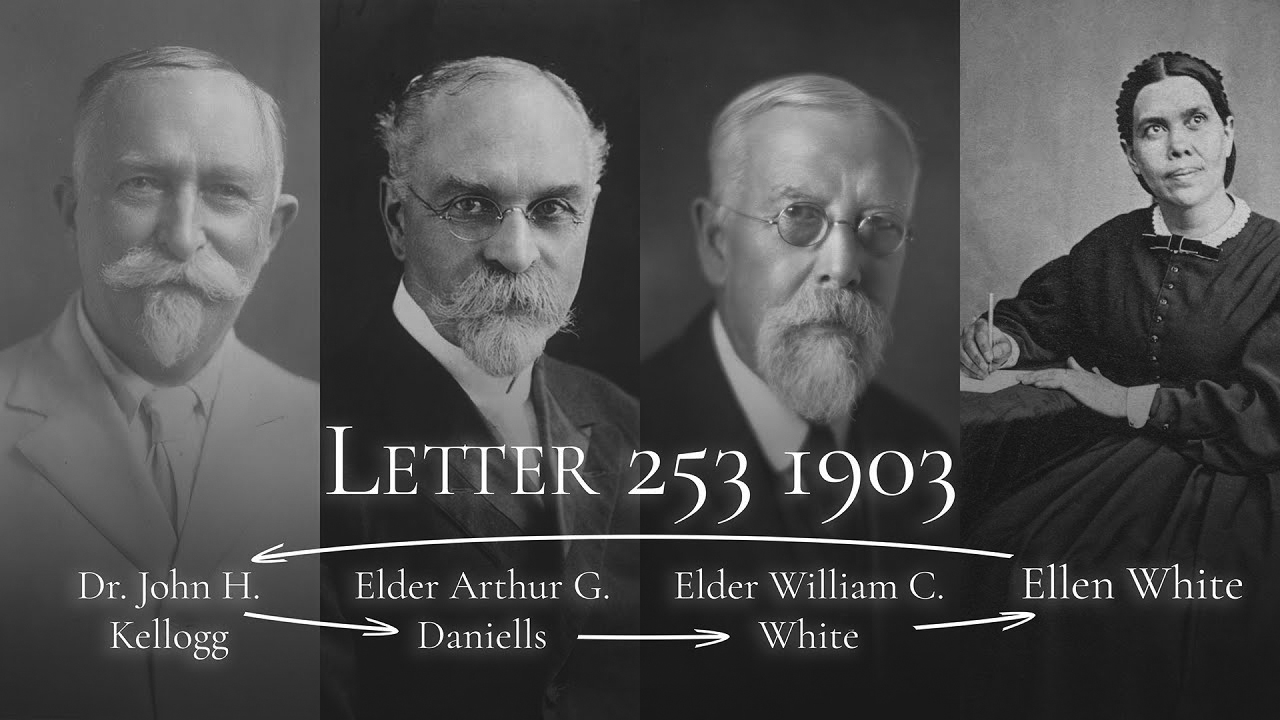
\includegraphics[width=1\linewidth]{images/correspondance.jpg}
    \caption*{Łańcuch korespondencji pomiędzy A. G. Daniellsem, W. C. White'em, Ellen White i dr. Johnem H. Kelloggiem.}
    \label{fig:corespondance}
\end{figure}

Oto dowód, że siostra White była zaznajomiona z zamiarami dr. Kellogga dotyczącymi korekty \textit{The Living Temple} oraz jego wiarą w doktrynę o Trójcy. Według słów Williama wypowiedziała się bardzo stanowczo w tej sprawie. Uznała to za bezowocne przedsięwzięcie. Z tego powodu konieczne było wydanie wkrótce specjalnego Świadectwa. I tak się stało. W ten sposób w 1904 roku opublikowano \textit{Testimonies for the Church Containing Letters to Physicians and Ministers Instruction to Seventh-Day Adventists}, zawierające listy do lekarzy i kaznodziejów związanych z kryzysem Kellogga.

Mówiąc: \othersnodot{\textbf{\underline{Matka i ja} właśnie przeczytaliśmy Twój list z \underline{29 października}}}, William zaświadczył, że siostra White była w pełni świadoma zamiarów Kellogga i jego trynitarnych przekonań. Po przeczytaniu listu Daniellsa napisała bezpośrednią odpowiedź do dr. Kellogga. Ten list to \textit{Lt253-1903}. Jest to bardzo znaczący i odkrywczy list, ponieważ jasno pokazuje, jak prorokini odnosiła się do doktryny o Trójcy. Podkreśliła doktrynę o \emcap{osobowości Boga} zawartą w \emcap{Fundamentalnych Zasadach}. Istnieją uderzające podobieństwa między tym listem a dziesiątym rozdziałem \textit{Special Testimonies}, „Fundament naszej wiary”.

\begin{titledpoem}
    \stanza{
        W „Świątyni” Kelloga sidło leżało, \\
        Przedstawienie Boga White nie pasowało. \\
        Jego słowa na temat osobowości Boga \\
        Były sofizmatami wręcz prosto od wroga.
    }

    \stanza{
        Nie będą naprawione żadne błędy stare \\
        Przez lekką korektę czy też w Trójcę wiarę. \\
        Gdyż osobowość Boga wyraźna i czysta — \\
        W tę prawdę winien wierzyć każdy adwentysta.
    }

    \stanza{
        Pomimo zastawionych sideł przeciwnika \\
        Niech prawda o Bogu z oczu nam nie znika. \\
        Fundament nasz musi bezpieczny pozostać \\
        I wsparty przez Biblię na wieki się ostać.
    }
\end{titledpoem}

           % Chapter 4
\qrchapter{https://forgottenpillar.com/rsc/pl-fp-chapter5}{Łatane teorie — Lt253-1903}

\egwnodot{Drogi Bracie,}

\egwnogap{\textbf{muszę Ci powiedzieć, że Twoje poglądy na temat niektórych kwestii \underline{były i są całkowicie błędne}.} Chciałabym, żebyś mógł dostrzec swoje błędy. \textbf{Książka «The Living Temple» \underline{nie powinna być łatana}, a po wprowadzeniu kilku zmian polecana i wychwalana jako wartościowa publikacja}. Lepiej byłoby przedstawić części dotyczące fizjologii w innej książce pod innym tytułem. \textbf{Kiedy pisałeś tę książkę}, \textbf{nie byłeś pod natchnieniem Bożym}. Był przy Tobie ten, który skłonił Adama do patrzenia na Boga w fałszywym świetle. Twoje całe serce potrzebuje przemiany oraz gruntownego i pełnego oczyszczenia}[Lt253-1903.1; 1903][https://egwwritings.org/read?panels=p9980.7]

\egwnogap{\textbf{Mój Bracie, nie pozwól się oddzielić od braci w służbie, którzy ostrzegają Cię przed niebezpieczeństwem. Ci, którzy wiernie i szczerze wytykają Ci Twoje błędy, są Twoimi najlepszymi przyjaciółmi.} Jest mi bardzo, bardzo przykro z powodu Twoich współpracowników medycznych. Byli oni niewierni Bogu i nieszczerzy wobec Ciebie, nie mówiąc Ci z uprzejmością, ale i  stanowczością, gdzie postępowałeś niesłusznie}[Lt253-1903.2; 1903][https://egwwritings.org/read?panels=p9980.8]

\egwnogap{Jest wiele rzeczy, które musisz przezwyciężyć, zanim będziesz mógł być zbawiony. W sercu, które nie jest prowadzone przez Boga, jest coś, co prowadzi do pragnienia podążania niewłaściwym kursem. Ludzi, którzy wiernie mówią Ci prawdę, wskazując Twoje błędy, uważasz za swoich wrogów. Ale często są oni Twoimi najlepszymi przyjaciółmi i mówiąc Ci, gdzie błądziłeś, wypełniali bardzo nieprzyjemny obowiązek. Słudzy Pańscy nie mają schlebiać Twojej dumie; nie mają milczeć i bać się powiedzieć: «Dlaczego tak czynisz?». Mają wiernie ostrzegać Cię przed niebezpieczeństwem}[Lt253-1903.3; 1903][https://egwwritings.org/read?panels=p9980.9]

\egwnogap{\textbf{Mój mąż, starszy Joseph Bates, ojciec Pierce, starszy Edson i wielu innych, którzy byli gorliwi, szlachetni i prawi, byli pośród tych, którzy po upływie czasu w 1844 roku szukali prawdy}. \textbf{Na naszych ważnych spotkaniach ci mężowie zbierali się razem i szukali prawdy jak ukrytego skarbu}. Spotykałam się z nimi i studiowaliśmy, i modliliśmy się żarliwie; czuliśmy bowiem, że musimy poznać Bożą prawdę. Często pozostawaliśmy razem do późnej nocy, a czasami przez całą noc, modląc się o światło i studiując Słowo. Gdy pościliśmy i modliliśmy się, zstępowała na nas wielka moc. Nie mogłam jednak pojąć rozumowania braci. Mój umysł był jakby zablokowany i nie mogłam zrozumieć tego, co studiowaliśmy. Wtedy Duch Boży zstępował na mnie, zabierano mnie w widzeniu i otrzymywałam jasne wyjaśnienie fragmentów, które studiowaliśmy, wraz z pouczeniem co do stanowiska, jakie powinniśmy zająć odnośnie prawdy i obowiązku. Działo się tak wielokrotnie. \textbf{Linia prawdy rozciągająca się od tamtego czasu do momentu, gdy wejdziemy do miasta Bożego, została wyraźnie przede mną nakreślona} i przekazałam braciom i siostrom pouczenie, które dał mi Pan. Wiedzieli oni, że gdy nie byłam w widzeniu, nie mogłam zrozumieć tych spraw, i przyjmowali dane mi objawienia jako światło bezpośrednio z nieba. \textbf{W ten sposób zostały pewnie ustanowione główne punkty naszej wiary, które wyznajemy dzisiaj}. \textbf{\underline{Punkt po punkcie} został jasno zdefiniowany i wszyscy bracia doszli do zgodności}}[Lt253-1903.4; 1903][https://egwwritings.org/read?panels=p14068.9980010]

\egwnogap{\textbf{Cała społeczność wierzących była zjednoczona w prawdzie}. \textbf{Byli tacy, którzy przychodzili z dziwnymi doktrynami, ale nigdy nie baliśmy się by im sprostać. Nasze doświadczenie zostało cudownie utwierdzone przez objawienia Ducha Świętego}}[Lt253-1903.5; 1903][https://egwwritings.org/read?panels=p9980.11]

\egwnogap{Przez dwa lub trzy lata mój umysł pozostawał zamknięty na Pisma. W 1846 roku wyszłam za mąż za starszego Jamesa White’a. Po jakimś czasie od narodzin mojego drugiego syna byliśmy w wielkiej rozterce odnośnie do pewnych punktów doktryny. Modliłam się do Pana, aby otworzył mój umysł, bym mogła zrozumieć Jego Słowo. Nagle wydało się, że zostałam otoczona jasnym, pięknym światłem, i od tamtej pory \textbf{Pisma są dla mnie otwartą księgą}}[Lt253-1903.6; 1903][https://egwwritings.org/read?panels=p14068.9980012]

\egwnogap{Byłam wtedy w Paris, w stanie Maine. Stary ojciec Andrews był bardzo chory. Od pewnego czasu bardzo cierpiał z powodu reumatycznego zapalenia stawów. Nie mógł się poruszać bez intensywnego bólu. Modliliśmy się za niego. Położyłam ręce na jego głowie i powiedziałam: «Ojcze Andrews, Pan Jezus Cię uzdrawia». Został uzdrowiony natychmiast. Wstał i chodził po pokoju, chwaląc Boga i mówiąc: «Nigdy wcześniej nie widziałem czegoś takiego. Aniołowie Boży są w tym pokoju». Chwała Boża została objawiona. \textbf{Światło zdawało się świecić w całym domu, a ręka anioła została położona na mojej głowie. Od tamtego czasu aż do teraz jestem w stanie rozumieć Słowo Boże}}[Lt253-1903.7; 1903][https://egwwritings.org/read?panels=p9980.13]

\egwnogap{\textbf{Po upływie czasu byliśmy prześladowani i okrutnie oczerniani. Mężczyźni i kobiety, którzy popadli w fanatyzm, zarzucali nam błędne teorie}. Kazano mi udać się w miejsca, gdzie ci ludzie głosili te błędne teorie, a gdy tam szłam, cudownie ukazywała się moc Ducha w napominaniu błędów, które się wkradały. \textbf{\underline{Sam szatan, w osobie człowieka}, działał, aby obrócić wniwecz moje świadectwo dotyczące stanowiska, które teraz, jak wiemy, jest potwierdzone przez Pismo}}[Lt253-1903.8; 1903][https://egwwritings.org/read?panels=p9980.14]

\egwnogap{\textbf{Dokładnie takie teorie, jakie przedstawiłeś w «The Living Temple», były przedstawiane wtedy}. \textbf{Te subtelne, zwodnicze sofizmaty raz za razem próbowały się wśród nas zadomowić. \underline{Lecz zawsze miałam do złożenia to samo świadectwo, które składam teraz odnośnie do osobowości Boga}}}[Lt253-1903.9; 1903][https://egwwritings.org/read?panels=p14068.9980015]

\egwnodotnogap{W «Early Writings», str. 60, 66, 67\footnote{Wydaje się, że podane strony są nieprawidłowe. Wspomniane akapity można znaleźć w \textit{Early Writings} na stronach \href{https://egwwritings.org/read?panels=p28.462&index=0}{70.2}, \href{https://egwwritings.org/read?panels=p28.490&index=0}{77} i \href{https://egwwritings.org/read?panels=p28.390&index=0}{54.2}.}, znajdują się następujące stwierdzenia:}[Lt253-1903.10; 1903][https://egwwritings.org/read?panels=p9980.16]

\egwnogap{14 maja 1851 roku ujrzałam piękno i urok Jezusa. Gdy patrzyłam na Jego chwałę, nie przyszło mi do głowy, że kiedykolwiek mogłabym zostać oddzielona od Jego obecności. \textbf{Zobaczyłam światło wychodzące z chwały, która otaczała Ojca}, a gdy zbliżyło się do mnie, moje ciało drżało i trzęsło się jak liść. Myślałam, że jeśli podejdzie bliżej, przestanę istnieć; ale światło mnie minęło. \textbf{Wtedy mogłam w pewnym stopniu pojąć, z jak wielkim i strasznym \underline{Bogiem} mamy do czynienia}}[Lt253-1903.11; 1903][https://egwwritings.org/read?panels=p9980.17]

\egwnogap{Często widziałam \textbf{kochanego Jezusa, że jest osobą}. \textbf{Zapytałam Go, czy Jego Ojciec jest osobą i czy ma \underline{postać} jak On}. Jezus odpowiedział: «\textbf{Jestem dokładnym obrazem osoby Mojego Ojca!}» [Hbr 1:3]}[Lt253-1903.12; 1903][https://egwwritings.org/read?panels=p14068.9980018]

\egwnogap{\textbf{Często widziałam, że spirytualistyczny pogląd odebrał całą chwałę niebu, a w wielu umysłach tron Dawida i urocza osoba Jezusa zostały spalone w ogniu spirytualizmu}. Widziałam, że pewni ludzie, którzy zostali zwiedzeni i wprowadzeni w ten błąd, zostaną wyprowadzeni na światło prawdy, \textbf{ale będzie prawie niemożliwe, aby całkowicie uwolnili się od zwodniczej mocy spirytualizmu. Tacy powinni skrupulatnie wyznać swoje błędy i na zawsze je porzucić}}[Lt253-1903.13; 1903][https://egwwritings.org/read?panels=p14068.9980019]

\egwnogap{\textbf{Wśród naszego ludu \underline{wkrada się} nurt spirytualizmu i \underline{podkopie on wiarę} tych, którzy mu ulegną, sprawiając, że dadzą posłuch zwodniczym duchom i naukom demonów}. Błędy będą przedstawiane w przyjemny i pochlebny sposób. Wróg pragnie odwrócić umysły naszych braci i sióstr od dzieła przygotowania ludu, który by się ostał w tych ostatnich dniach}[Lt253-1903.14; 1903][https://egwwritings.org/read?panels=p9980.21]

\egwnogap{Zostałam pouczona, aby ostrzec naszych braci i siostry, \textbf{by nie dyskutowali o naturze naszego Boga}. Wielu ciekawskich, którzy próbowali otworzyć arkę przymierza, aby zobaczyć, co jest w środku, zostało ukaranych za swoją zuchwałość. \textbf{Nie możemy mówić, że Pan Bóg niebios jest w liściu lub w drzewie, ponieważ Go tam nie ma. \underline{On zasiada na swoim tronie w niebiosach}}}[Lt253-1903.15; 1903][https://egwwritings.org/read?panels=p14068.9980022]

\egwnogap{Dzieło Stwórcy widziane w przyrodzie objawia Jego moc. Lecz przyroda nie jest ponad Bogiem ani Bóg nie jest w przyrodzie, jak niektórzy Go przedstawiają. Bóg stworzył świat, ale świat nie jest Bogiem; jest tylko dziełem Jego rąk. \textbf{Przyroda objawia dzieło prawdziwego, \underline{osobowego Boga}, pokazując, że Bóg jest i że nagradza tych, którzy go szukają}}[Lt253-1903.16, 1903][https://egwwritings.org/read?panels=p9980.23]

\egwnogap{Mogłabym wiele powiedzieć o świątyni; o arce zawierającej prawo Boże; o wieku arki, które jest przebłagalnią; o aniołach po obu stronach arki; i o innych rzeczach związanych z niebiańską świątynią i wielkim dniem pojednania. Mogłabym wiele powiedzieć o tajemnicach nieba; lecz moje usta są zamknięte. Nie mam ochoty próbować ich opisywać}[Lt253-1903.17; 1903][https://egwwritings.org/read?panels=p9980.25]

\egwnogap{\textbf{Nie ośmieliłabym się mówić o Bogu tak, jak Ty o Nim mówiłeś}. On jest wysoki i wywyższony, a Jego chwała wypełnia niebiosa. «Głos Pana jest potężny; wstrząsa cedrami Libanu. \textbf{Pan jest w swoim świętym przybytku}. Niech cała ziemia zamilknie przed Nim». [Patrz Ps 29:5, Ha 2:20]}[Lt253-1903.18; 1903][https://egwwritings.org/read?panels=p14068.9980026]

\egwnogap{\textbf{Mój Bracie, gdy kusi Cię, aby mówić o Bogu, \underline{gdzie On jest lub czym jest}, pamiętaj, że w tej kwestii milczenie jest elokwencją}. Zdejmij buty z nóg; bo ziemia, na której stawiasz swoje niedbałe, nieuświęcone stopy, jest święta}[Lt253-1903.19; 1903][https://egwwritings.org/read?panels=p14068.9980027]

\egwnogap{\textbf{Jestem pouczona, aby powiedzieć, że w Słowie Bożym nie ma niczego, co potwierdzałoby Twoje spirytualistyczne teorie. Czy nie zechcesz od razu się ich wyrzec? Twój umysł zajmował się nimi przez długi czas, ale nie miały one uświęcającego, oczyszczającego ani uszlachetniającego wpływu na Twoje życie. Pan nie ma pożytku z tych teorii i nie chce, aby Jego lud ich bronił lub je propagował}}[Lt253-1903.20; 1903][https://egwwritings.org/read?panels=p9980.28]

\egwnogap{\textbf{Ojciec, Wszechwiedzący, stworzył świat przez Chrystusa Jezusa}. Chrystus jest światłością świata, drogą do życia wiecznego. Jego, Pomazańca, Bóg dał, aby dokonał przebłagania za grzechy świata. Musisz zrozumieć, że jeśli nie uwierzysz w to przebłaganie i nie będziesz wiedział, że zostałeś kupiony za cenę krwi jednorodzonego Syna Bożego, z pewnością zostaniesz związany ze złym. \textbf{Jeżeli nadal będziesz pielęgnował teorie, które dotąd pielęgnowałeś, zostaniesz wydany na pastwę pokus szatana}. On toczy grę o Twoją duszę. Pozostań jeszcze trochę związany z nim, a możesz być pewien, że stracisz swoją duszę}[Lt253-1903.21; 1903][https://egwwritings.org/read?panels=p14068.9980029]

\egwnogap{Twierdząc, że nasze instytucje są bezdenominacyjne, postawiłeś naszych ludzi i naszą pracę w fałszywej pozycji. Zostałeś poprowadzony straszną ścieżką, której niebezpieczeństw nie znałeś, ale możesz je kiedyś zobaczyć. Nie jest jeszcze za późno, aby naprawić błędy. Jest dla Ciebie nadzieja. \textbf{Podążałeś za wrogiem krok po kroku, starając się zgłębić tajemnice zbyt wysokie i święte dla Twojego pojmowania}. \textbf{Potem w Twoim nauczaniu Święty został sprowadzony do poziomu ludzkich \underline{naukowych, spirytualistycznych idei}}. Chodziłeś krętymi ścieżkami. Utraciłeś moralny obraz Boga. Jednak jest dla Ciebie nadzieja. Wciąż możesz skierować swoje stopy na właściwą ścieżkę. Czy teraz nie wyprostujesz ścieżek dla swoich stóp, aby to, co chrome, nie zeszło z drogi? Czy teraz odmówisz zasiania choćby jednego więcej ziarna sceptycyzmu i sofistyki w umysłach innych? Czy teraz przyjdziesz do Chrystusa, aby zostać uzdrowiony?}[Lt253-1903.22; 1903][https://egwwritings.org/read?panels=p14068.9980030]

\egwnogap{\textbf{Wahałam się i zwlekałam z wysłaniem tego, do czego napisania pobudził mnie Duch Pana}. Nie chciałam być zmuszona do przedstawienia szatańskiego wpływu tych sofizmatów. Lecz jeżeli nie nastąpi zdecydowana zmiana w Tobie i Twoich współpracownikach, będę musiała to zrobić, żeby uchronić innych od podążania ścieżką, którą Ty podążałeś. Będę musiała być posłuszna rozkazowi danemu mi przez Boga: «\textbf{Przeciwstaw się temu}». To jedyna rzecz, którą mogę zrobić}[Lt253-1903.23; 1903][https://egwwritings.org/read?panels=p9980.31]

\egwnogap{Przedstawiam Ci rzeczy, które Pan mi przedstawił. Jest wielka praca do wykonania. Musimy podjąć się tej pracy ze zrozumieniem, modląc się, wierząc i przyjmując Ducha Świętego. Tylko w ten sposób możemy wykonać powierzoną nam pracę. \textbf{Bóg wymaga ode mnie, abym świadczyła przeciwko «The Living Temple»}. Bez względu na to, co Twoi współpracownicy powiedzą o tej książce, \textbf{raz na zawsze zajmuję stanowisko, że jest ona sidłem}. \textbf{Nasz lud jako całość nie zjednoczy się wokół \underline{teorii}, które zacząłeś przedstawiać w tej książce}. \textbf{Możesz uznać to za ostatecznie przesądzone}. \textbf{Jako lud będziemy stać niewzruszenie \underline{na platformie, która wytrzymała próby i doświadczenia}. Będziemy trzymać się \underline{pewnych filarów naszej wiary}. \underline{Zasady prawdy}, które Bóg nam objawił, są naszym jedynym fundamentem. One uczyniły nas tym, czym jesteśmy. Te nowe, fantazyjne teorie są czarujące i zwodnicze. Zagrażają wiecznemu dobru duszy. Pisma ich nie potwierdzają}. Przyodziani w chrześcijańską zbroję, obuci w gotowość ewangelii pokoju, będziemy stać \textbf{niewzruszenie przeciwko tym zwodniczym teoriom}. Możesz przekręcać i wykrzywiać Słowo Boże ku swemu własnemu zatraceniu, ale błagam Cię, nie rób tego}[Lt253-1903.24; 1903][https://egwwritings.org/read?panels=p9980.32]

\egwnogap{\textbf{Niebo nie jest parą. Jest miejscem}. \textbf{Chrystus poszedł przygotować mieszkania dla tych, którzy Go miłują}, tych, którzy w posłuszeństwie Jego przykazaniom wychodzą ze świata i są oddzieleni. Zasady nieba muszą stać się naszym doświadczeniem, aby można było nas odróżnić od świata. \textbf{Musi być wyraźny kontrast między nami a światem; jesteśmy bowiem ludem nazwanym przez Boga}}[Lt253-1903.25; 1903][https://egwwritings.org/read?panels=p14068.9980033]

\egwnogap{Pan dał Ci możliwość naprawienia sytuacji. \textbf{Cieszę się, że zacząłeś to robić. Nie myśl, że nie mamy prawa próbować naprawić Twoich błędów i ich skutków. Dopóki Bóg daje mi oddech i zleca mi używanie pióra i głosu do odpierania tego zła, które pojawiło się wśród nas, będę pełnić swoją rolę w tej walce. Odkąd miałam siedemnaście lat, musiałam toczyć tę bitwę przeciwko fałszywym teoriom w obronie prawdy}. \textbf{Historia naszego doświadczenia z przeszłości jest trwale zapisana w moim umyśle i jestem przeświadczona, że \underline{żadne teorie w rodzaju tych, które przyjmowałeś}, nie wejdą w nasze szeregi}. Jeżeli nie będziesz chciał się zmienić i będziesz starał się prowadzić swoich współpracowników za sobą, a oni odważą się podążać za Twoim przewodnictwem, odpowiedzialność spoczywa na Tobie i na nich, nie na mojej duszy}[Lt253-1903.26, 1903][https://egwwritings.org/read?panels=p9980.34]

\egwnogap{\textbf{Mówię stanowczo, abyś wiedział, że dopóki nie nastąpi w Tobie zdecydowana przemiana, nie może być nadziei na zjednoczenie między Tobą a tymi, którzy trzymają się swoich początkowych wierzeń mocno aż do końca}. To Ty utworzyłeś podział. \textbf{\underline{Musimy stanowczo bronić prawd, które Pan dał nam jako filary naszej wiary}}}[Lt253-1903.27; 1903][https://egwwritings.org/read?panels=p9980.35]

\egwnogap{Błagam Cię, zwróć się do Pana z pełnym postanowieniem serca, zanim będzie na zawsze za późno. Oddziel się od wpływów, które oddzieliły Cię od twoich braci zaangażowanych w służbę ewangelii i od ludu, który Bóg prowadzi. \textbf{\underline{Łatane teorie} nie mogą być przyjęte przez lojalnych wobec wiary i \underline{zasad}, które wytrzymały wszelki sprzeciw szatańskich wpływów}}[Lt253-1903.28; 1903][https://egwwritings.org/read?panels=p14068.9980036]

\egwnogap{Jeśli opróżnisz się ze wszystkiego, co oddzieliło Cię od Chrystusa, i przyjmiesz Zbawiciela do swojego serca, Twój charakter zostanie przemieniony. Odłóż na jakiś czas obowiązki i udaj się gdzieś z kilkoma swoimi braćmi, i razem z nimi badaj Pisma. Ukórz swoje serce przed Panem i dokonaj gruntownej pracy ku pokucie. \textbf{Religia Chrystusa jest duchowym zaczynem, który ma być wprowadzony do serca. To zmienia życie i charakter}. Ta religia jest niebiańską zasadą, widoczną w życiu i zachowaniu chrześcijanina. Objawia się w chrześcijańskiej czystości. Miłość Chrystusa jest widoczna w czułości i łasce uświęconego człowieczeństwa. To przez Słowo, które stało się ciałem, jesteśmy zbawieni. Nasze odkupienie zostało dokonane \textbf{nie przez to, że Syn Boży pozostał w niebie, ale przez to, że Syn Boży stał się wcielony — przyjął na siebie człowieczeństwo i przyszedł na ten świat}. W ten sposób przyniesiono nam życie wieczne. To, czego autorytet, przykazania i obietnice nie mogły dokonać, Bóg uczynił, przychodząc na ten świat w podobieństwie grzesznego ciała}[Lt253-1903.29; 1903][https://egwwritings.org/read?panels=p9980.37]

\egwnogap{Chrystus przyszedł na ziemię, aby żyć jako człowiek wśród ludzi, nie po to, by zostać zepsutym przez ludzką słabość, ale by umieścić w umysłach ludzi zasady prawdy, które nigdy nie zostaną wymazane, ponieważ są wiecznie prawdziwe. Przyszedł, aby przynieść nowe życie upadłym istotom ludzkim — doskonałość, która nie mogła być splamiona ani zniszczona przez grzech}[Lt253-1903.30; 1903][https://egwwritings.org/read?panels=p9980.38]

\egwnogap{\textbf{Mój Bracie, muszę Ci powiedzieć, że nie zdajesz sobie sprawy, dokąd zmierzają Twoje kroki}. Związałeś się z tymi, którzy należą do armii wielkiego odstępcy. \textbf{Twój umysł stał się ciemny jak Egipt}. \textbf{Jeśli upadniesz na Skałę i zostaniesz skruszony}, Chrystus Cię przyjmie. Stoisz jednak na terenie wroga, wykonując jego pracę. \textbf{Religijny świat szybko podąża tą samą drogą, którą Ty idziesz. Jeśli będziesz dalej nią podążał, będziesz miał mnóstwo towarzystwa. Lecz jaki będzie koniec?}}[Lt253-1903.31; 1903][https://egwwritings.org/read?panels=p14068.9980039]

\egwnogap{Tak długo chodziłeś w ciemności, tak długo podążałeś własną drogą, że możesz być silnie kuszony, by oprzeć się temu apelowi, który wystosowuję. Gdyby nie to, że chodzi o Twoje \textbf{wieczne dobro}, nie mówiłabym Ci o tej sprawie. Mogłoby się wydawać, że napisałam wystarczająco dużo, że nie ma potrzeby dalszego narzucania Ci tego tematu. \textbf{Lecz mówię Ci zgodnie z prawdą, że doskonale rozumiem, co robię}. Otrzymałeś wystarczające światło. Ale od kilku lat nie zważasz na to światło. Gdybyś chciał wiedzieć, co Pan powiedział, mógłbyś się dowiedzieć; \textbf{masz bowiem książki, które zostały napisane pod przewodnictwem Jego Ducha}. Otrzymałeś wszystkie wskazówki, o jakie można było prosić, aby znaleźć właściwą drogę. Posłano Ci bezpośrednie światło. Lecz uznałeś to za mniej ważne niż swoje własne plany i zamysły. Gdybyś zważał na posłane Ci świadectwa, książka «The Living Temple» nigdy nie zostałaby napisana}[Lt253-1903.32; 1903][https://egwwritings.org/read?panels=p14068.9980040]

\egwnogap{Czy nie podejmiesz gruntownego, zdecydowanego, chrystusowego wysiłku, aby przełamać czar, który rzucił na Ciebie szatan? Miał dotąd wielką władzę nad Twoim umysłem i kierował Cię na złe drogi. Myśli, że może teraz nad Tobą panować. Czy nie pokonasz go i nie rozczarujesz?}[Lt253-1903.33; 1903][https://egwwritings.org/read?panels=p9980.41]

\egwnogap{Piszę do Ciebie jak do syna. Odłącz się od wroga — oskarżyciela braci. Powiedz mu: «Idź precz ode mnie, szatanie. Popełniłem ciężki grzech, słuchając twoich sugestii. Nie będę już ich więcej słuchał». Błagam Cię, dla dobra Twojej duszy, oprzyj się kusicielowi, aby uciekł od Ciebie. Zbliż się do Boga, a On przybliży się do Ciebie. \textbf{Stracisz niebo, jeśli nie upadniesz na Skałę i nie zostaniesz skruszony}}[Lt253-1903.34; 1903][https://egwwritings.org/read?panels=p9980.42]

Wiele spraw w tym liście do dr. Kellogga pozostaje niewypowiedzianych, ale stają się jasne, gdy zrozumiemy kontekst. Ellen White przeczytała list od brata Daniellsa wyrażający, jak dr Kellogg chciał poprawić \textit{The Living Temple}, ponieważ \othersnodot{przemyślał tę sprawę i zaczął dostrzegać, że popełnił drobny błąd w \textbf{wyrażaniu} swoich poglądów}, i \othersnodot{że niedługo potem \textbf{zaczął wierzyć w trójcę} i mógł teraz całkiem wyraźnie zobaczyć, gdzie tkwił cały problem, i wierzył, że może wyjaśnić sprawę w satysfakcjonujący sposób}. Kellogg wyznał, \othersnodot{że teraz wierzy \textbf{w Boga Ojca, Boga Syna i Boga Ducha Świętego}}. W odpowiedzi siostra White osobiście napisała do niego: \egwinline{Książka «The Living Temple» \textbf{nie powinna być łatana}, a po wprowadzeniu kilku zmian polecana i wychwalana jako wartościowa publikacja}. Jak Kellogg chciał załatać swoją książkę? Według świadectwa A. G. Daniellsa myślał o zmianie kilku wyrażeń poprzez wyraźne stwierdzenie swojego trynitarnego poglądu. Ale wyrażenie poglądów nie było prawdziwym problemem — były nim same poglądy. Siostra White nie szczędziła mu nagany za jego poglądy o Bogu, które były poglądami \textit{trynitarnymi}. Powiedziała mu, iż jest \egwinline{\textbf{przeświadczona, że \underline{żadne teorie w rodzaju tych, które on przyjmuje}, nie wejdą w nasze szeregi}}. To bardzo mocne stwierdzenie. Czy możliwe, że skoro Kellogg wyznał, iż przyjmuje doktrynę o Trójcy, siostra White włączyła ją również w swoje oświadczenie? Wydaje się to nie do pomyślenia, gdyż ta doktryna jest dziś w naszych szeregach. Ale jej oświadczenie faktycznie wskazuje na Trójcę, gdy powiedziała: \egwinline{\textbf{Łatane teorie} nie mogą być przyjęte przez lojalnych wobec \textbf{wiary i zasad}, które wytrzymały wszelki sprzeciw szatańskich wpływów}. Kellogg chciał załatać \textit{The Living Temple} przez wyraźne nadmienienie doktryny o Trójcy. Dlaczego siostra White była zdecydowana, by trzymać tę doktrynę z dala od naszych szeregów, choć jednak jest ona dziś w naszych szeregach? Uczciwie należy zauważyć, że Trójca nie była częścią wiary Adwentystów Dnia Siódmego w jej czasach i weszła do naszych szeregów później. Dziś wielu twierdzi, że to dzięki jej pracom Trójca jest częścią naszych wierzeń, ale reakcja Ellen White i jej odpowiedź na wiarę Kellogga w nią pokazuje, jak ona traktowała taką doktrynę. Czego możemy się z tego nauczyć?

Rozważany w swoim kontekście, ten list rzuca nowe światło na kontrowersję dotyczącą Kellogga i pokazuje, jak powinniśmy podchodzić do doktryny o Trójcy. Pierwszą rzeczą, którą kwestionujemy, jest to, dlaczego siostra White nigdy nie użyła słowa „Trójca” w swoich pismach, nawet gdy bezpośrednio odnosiła się do tej doktryny. W innym miejscu odpowiada:

\egw{Zostałam przestrzeżona, aby nie wchodzić w spory \textbf{dotyczące kwestii}, które \textbf{\underline{pojawią się}} w związku z \textbf{tymi sprawami, ponieważ spory \underline{mogłyby doprowadzić ludzi do uciekania się do wybiegów, a ich umysły zostałyby odwiedzione od prawdy Słowa Bożego do przypuszczeń i domysłów}}. \textbf{Im więcej dyskutuje się o wymyślnych teoriach, tym \underline{mniej ludzie będą wiedzieć o Bogu i o prawdzie, która uświęca duszę}}}[Lt232-1903.41; 1903][https://egwwritings.org/read?panels=p14068.10197050]

To bardzo ważna lekcja i zasada, której uczy nas tutaj siostra White. Kiedy zrodził się spór wokół teorii Kellogga, nie zagłębiała się w same teorie, ponieważ to odprowadzałoby umysły ludzi od prawdy Słowa Bożego do przypuszczeń i domysłów. Zamiast tego, kierowała umysły ludzi ku prawdzie, która uświęca duszę. Prowadziła przykładem, co widać tutaj w jej liście do dr. Kellogga. Ta prawda, ku której kierowała umysły ludzi, była prawdą o \emcap{osobowości Boga}. Zganiła Kellogga za jego teorie, ale, co bardzo ważne, właściwie identyfikujemy te teorie poprzez ich kontekst i jej domyślne ich wyrażenie.

Widzimy, że pokazała kontrast między Trójcą a \emcap{osobowością Boga}. Pokazała kontrast między starymi zasadami naszej wiary a nowymi teoriami. Najpierw skierowała nasze umysły z powrotem do początku naszego duchowego dziedzictwa, \egwinline{po upływie czasu w 1844 roku}, gdy jej mąż James White, Joseph Bates, ojciec Pierce, starszy Edson i wielu innych, którzy byli gorliwi, szlachetni i prawi, szukali prawdy. Wskazała na wspaniałe i potężne doświadczenia, jak główne punkty naszej wiary, wyznawane w 1903 roku, zostały pewnie ustanowione. \egwinline{\textbf{W ten sposób zostały pewnie ustanowione \underline{główne punkty naszej wiary}}, które wyznajemy dzisiaj}. \egwinline{\textbf{\underline{Punkt po punkcie} został jasno zdefiniowany i wszyscy bracia doszli do zgodności}}. \egwinline{\textbf{Cała społeczność wierzących była zjednoczona w prawdzie}}. Oczywiście z kontekstu 10. rozdziału \textit{Special Testimonies} wiemy, że te doświadczenia wyjaśniają, \egwinline{\textbf{jak mocno został położony fundament naszej wiary}}[SpTB02 56.4; 1904][https://egwwritings.org/read?panels=p417.288]. Ten fundament jest wyrażony w \emcap{Fundamentalnych Zasadach}\footnote{\href{https://static1.squarespace.com/static/554c4998e4b04e89ea0c4073/t/59d17e24c027d84167e17617/1506901547915/SDA-YB1905+\%28P.+188-192\%29.pdf}{Yearbook Of Seventh-day Adventist denomination 1905, str. 188--192}}. Ten fundament jest prawdą, która \egwinline{\textbf{\underline{punkt po punkcie} została odkryta przez pełne modlitwy studium i potwierdzona przez cudotwórczą moc Pana}}. Bóg \egwinline{\textbf{wzywa nas, abyśmy \underline{mocno trzymali się}, z uściskiem wiary, \underline{fundamentalnych zasad}, które są \underline{oparte na niepodważalnym autorytecie}}}[SpTB02 59.1; 1904][https://egwwritings.org/read?panels=p417.299]. W świetle tych doświadczeń i prawdy wyrażonej w \emcap{fundamentalnych zasadach} \egwinline{\textbf{\underline{łatane teorie} nie mogą być przyjęte przez lojalnych wobec \underline{wiary} i \underline{zasad}, które wytrzymały wszelki sprzeciw szatańskich wpływów}}[Lt253-1903.28; 1903][https://egwwritings.org/read?panels=p14068.9980036]. Z historycznego zapisu tych braci, którzy byli gorliwi, szlachetni i prawi, mamy dowody, że oni również przeciwstawiali doktrynę o Trójcy prawdzie o \emcap{osobowości Boga}. James White w artykule w \textit{Review and Herald} wymienił \others{niektóre z popularnych bajek epoki}, mówiąc: \othersnodot{Tutaj możemy nadmienić \textbf{Trójcę, która \underline{pozbywa się osobowości Boga i Jego Syna Jezusa Chrystusa}}}[James White, Review \& Herald, 11 grudnia 1855, str. 85.15][http://documents.adventistarchives.org/Periodicals/RH/RH18551211-V07-11.pdf]. J. N. Andrews powiedział: \othersnodot{\textbf{Doktryna Trójcy, która została ustanowiona w Kościele przez sobór nicejski w 325 r. n.e. Ta doktryna \underline{niszczy osobowość Boga i Jego Syna Jezusa Chrystusa, naszego Pana}}...}. J. B. Frisbie w swoim artykule „\textit{Szabat dnia siódmego niezniesiony}” porównuje Boga szabatu z bogiem niedzieli; opisuje Boga szabatu w świetle \emcap{osobowości Boga} wyrażonej w pierwszym punkcie \emcap{Fundamentalnych Zasad}. Bóg niedzieli jest opisany jako \othersnodot{jedność tego Bóstwa, są trzy osoby jednej substancji, mocy i wieczności; Ojciec, Syn i Duch Święty}[J. B. Frisbie, Review \& Herald, 7 marca 1854, str. 50][http://documents.adventistarchives.org/Periodicals/RH/RH18540307-V05-07.pdf]. Wyjaśnił, jak doktryna o \emcap{osobowości Boga} stoi w konflikcie z doktryną o Trójcy, w ten sam sposób, jak Święty Szabat stoi w konflikcie z pogańskim kultem niedzieli. Również brat J. N. Loughborough spisał zastrzeżenia do doktryny o Trójcy w \textit{Adventist Review and Sabbath Herald}\footnote{\href{https://adventistdigitallibrary.org/adl-349160/advent-review-and-sabbath-herald-november-5-1861}{J. N. Loughborough, 5 października 1861, Review \& Herald, tom 18, str. 184, akap. 1-11}}. W innym wydaniu \textit{Review and Herald} opublikował artykuł „\textit{Czy Bóg jest osobą?}”, wyjaśniając stanowisko wiary Adwentystów Dnia Siódmego w sprawie \emcap{osobowości Boga}, wyrażone w pierwszym punkcie \emcap{Fundamentalnych Zasad}\footnote{\href{http://documents.adventistarchives.org/Periodicals/RH/RH18550918-V07-06.pdf}{J. N. Loughborough, 18 września 1855, Review \& Herald, tom 7, str. 6.}}. James White również wyjaśniał to samo stanowisko w swojej wielokrotnie drukowanej broszurze „\textit{Osobowość Boga}”\footnote{\href{https://egwwritings.org/?ref=en_PERGO.1.1&para=1471.3}{J. White, The Personality of God, 18 czerwca 1861.}}. To tylko kilka przykładów, gdzie pionierzy adwentyzmu wyjaśniali stanowisko w sprawie \emcap{osobowości Boga} wyrażone w pierwszym punkcie \emcap{fundamentalnych zasad}.

Siostra White zganiła Kellogga: \egwinline{\textbf{Lecz mówię Ci zgodnie z prawdą, że doskonale rozumiem, co robię}. \textbf{Otrzymałeś wystarczające światło}. Ale od kilku lat nie zważasz na to światło. Gdybyś chciał wiedzieć, co Pan powiedział, mógłbyś się dowiedzieć; \textbf{\underline{masz bowiem książki}, które zostały napisane pod przewodnictwem Jego Ducha}. Otrzymałeś wszystkie wskazówki, o jakie można było prosić, aby znaleźć właściwą drogę. Posłano Ci bezpośrednie światło. Lecz uznałeś to za mniej ważne niż swoje własne plany i zamysły. Gdybyś zważał na posłane Ci świadectwa, książka «The Living Temple» nigdy nie zostałaby napisana}[Lt253-1903.32; 1903][https://egwwritings.org/read?panels=p14068.9980040]. Centralnym problemem kontrowersji związanej z dr. Kelloggiem była \egwinline{osobowość Boga i to, gdzie jest jego obecność}[SpTB02 51.3; 1904][https://egwwritings.org/read?panels=p417.262]. Dr. Kellogg miał dostęp do pism pionierów, książek oraz kościelnych \emcap{Fundamentalnych Zasad}, które były potwierdzone cudotwórczą mocą Ducha Świętego.

Siostra White przypomniała doświadczenia, jak \textit{główne punkty naszej wiary}, które były wyznawane w dawnych czasach, zostały pewnie ustanowione. \egwinline{\textbf{\underline{Punkt po punkcie}} \textbf{został jasno zdefiniowany i wszyscy bracia doszli do zgodności}}[Lt253-1903.4; 1903][https://egwwritings.org/read?panels=p14068.9980010]. Te główne punkty były \emcap{Fundamentalnymi Zasadami}, a \emcap{osobowość Boga} była jedną z nich. Ten punkt i świadectwo siostry White o nim pozostały takie same przez całe jej życie. Powiedziała: \egwinline{\textbf{\underline{Zawsze miałam to samo świadectwo do złożenia, które teraz składam odnośnie do osobowości Boga}}}[Lt253-1903.9; 1903][https://egwwritings.org/read?panels=p14068.9980015]. Z \textit{Early Writings} zacytowała swoje wizje niebiańskiej rzeczywistości. Przypomniała, jak miała przywilej być w obecności Boga, jak Bóg, otoczony światłem Swojej chwały, przeszedł obok niej. Nie widziała Boga z powodu światła, którym był otoczony; bała się Go, myśląc, że gdyby się do niej zbliżył, \egwinline{zostałaby unicestwiona}. Wtedy zobaczyła \egwinline{\textbf{kochanego Jezusa, że jest osobą}. \textbf{Zapytałam Go, czy Jego Ojciec jest osobą i ma \underline{postać taką jak} On}. Jezus odpowiedział: «\textbf{Jestem dokładnym obrazem osoby Mojego Ojca!}»}[Lt253-1903.12; 1903][https://egwwritings.org/read?panels=p14068.9980018]. Pytanie, które miała, brzmiało: \textit{Czy Bóg jest osobą, mającą postać jak Jezus}? Odpowiedź była twierdząca — z silną biblijną podstawą. Jej wizje nie były źródłem prawdy o \emcap{osobowości Boga}; raczej potwierdzały prawdę, którą pionierzy odkryli poprzez pilne studium Słowa Bożego.

Dlatego ich ostateczny wniosek dotyczący \emcap{osobowości Boga} brzmiał: \others{Że jest \textbf{jeden Bóg}, \textbf{osobowa, duchowa \underline{istota}}, \textbf{stwórca wszystkich rzeczy}, wszechmocny, wszechwiedzący i wieczny, nieskończony w mądrości, świętości, sprawiedliwości, dobroci, prawdzie i miłosierdziu; niezmienny i \textbf{wszędzie obecny przez swojego przedstawiciela, Ducha Świętego}. Ps 139:7; Że jest jeden Pan Jezus Chrystus, \textbf{Syn Wiecznego Ojca, ten, przez którego stworzył wszystkie rzeczy i przez którego one istnieją}...} \others{...i w końcowej części swojego dzieła jako kapłan, zanim obejmie swój tron jako król, dokona \textbf{wielkiego pojednania} za grzechy wszystkich takich, a ich grzechy zostaną wtedy wymazane (Dz 3:19) i wyniesione ze świątyni, jak pokazano w służbie kapłaństwa lewickiego, które zapowiadało i przedstawiało służbę naszego Pana w niebie. Patrz m.in. Kpł 16; Hbr 8:4--5; 9:6--7}[Pierwszy punkt i część drugiego punktu Fundamentalnych Zasad, 1905.]

Ellen White przypomniała dr. Kelloggowi o tym punkcie \emcap{fundamentalnych zasad}, stwierdzając: \egwinline{\textbf{Ojciec, Wszechwiedzący, stworzył świat przez Chrystusa Jezusa}. Chrystus jest światłością świata, drogą do życia wiecznego. \textbf{Jego, Pomazańca, Bóg dał, aby dokonał pojednania za grzechy świata}...}[Lt253-1903.21; 1903][https://egwwritings.org/read?panels=p14068.9980029]

Kwestia \emcap{osobowości Boga} dotyczy właściwości lub stanu Boga jako osoby. Pionierzy adwentyzmu dali na to odpowiedź, a Bóg zatwierdził ją przez pisma Ellen White: Bóg jest \textit{osobową duchową Istotą} i jest naszym niebiańskim Ojcem. Gdzie jest Jego obecność? \egwinline{\textbf{Nie możemy mówić, że Pan Bóg niebios jest w liściu lub w drzewie; bo Go tam nie ma. }\textbf{\underline{On zasiada na swoim tronie w niebiosach}}}[Lt253-1903.15; 1903][https://egwwritings.org/read?panels=p14068.9980022]. \\
Jego obecność jest na tronie w niebie. \\
\egwinline{\textbf{Niebo nie jest parą. Jest miejscem}. \textbf{Chrystus poszedł przygotować mieszkania dla tych, którzy Go miłują}, tych, którzy w posłuszeństwie Jego przykazaniom wychodzą ze świata i są oddzieleni...}[EGW, Lt253-1903.25; 1903][https://egwwritings.org/read?panels=p14068.9980033]. \\
\egwinline{... «Głos Pana jest potężny; wstrząsa cedrami Libanu. \textbf{Pan jest w swoim świętym przybytku}. Niech cała ziemia zamilknie przed Nim». [Patrz Ps 29:5; Ha 2:20]}[Lt253-1903.18; 1903][https://egwwritings.org/read?panels=p14068.9980026].

Według pionierów adwentyzmu i siostry White nasz niebiański Ojciec jest jednym Bogiem. Jest On osobową Duchową Istotą, obecną w niebie, na swoim tronie. Tron w niebie jest rzeczywistym, fizycznym tronem, na którym zasiada rzeczywista Osoba (Istota, mająca postać, tak jak Jezus) — nasz niebiański Ojciec. To miejsce jest rzeczywistym miejscem; nie jest parą ani żadnym innym duchowym wyobrażeniem.

\egwinline{\textbf{Często widziałam, że spirytualistyczny pogląd odebrał całą chwałę niebu, a w wielu umysłach tron Dawida i urocza osoba Jezusa zostały spalone w ogniu spirytualizmu}. Widziałam, że pewni ludzie, którzy zostali zwiedzeni i wprowadzeni w ten błąd, zostaną wyprowadzeni na światło prawdy, \textbf{ale będzie prawie niemożliwe, aby całkowicie uwolnili się od zwodniczej mocy spirytualizmu. Tacy powinni skrupulatnie wyznać swoje błędy i na zawsze je porzucić}}[Lt253-1903.13; 1903][https://egwwritings.org/read?panels=p14068.9980019].

Duchowe wyobrażenie osoby Boga jest błędnym poglądem. W Biblii mamy świadectwa o niebie, niebiańskim tronie i Bogu, który na nim zasiada. Jeśli przyjmiemy te świadectwa w ich oczywistym znaczeniu, wtedy doktryna o Trójcy nie może się ostać. Biblia i Duch Proroctwa przedstawiają jednego Boga w niebie, jako osobową istotę, mającą ciało i postać tak jak Jezus. Ten pogląd nie jest w harmonii z doktryną o Trójjedynym Bogu, ponieważ ta wymaga, aby Duch Święty był Istotą\footnote{W \hyperref[appendix:unauthenticated-reports]{Dodatku} można znaleźć więcej cytatów, które wykluczają, aby Duch Święty był istotą posiadającą fizyczne ciało i formę.}, mającą ciało i postać — ta idea zagroziłaby temu, że Duch Święty jest środkiem Ojca i Syna, przez który Oni są wszędzie obecni. Aby podtrzymać doktrynę o Trójcy, świadectwa dotyczące tronu Bożego i osoby Boga muszą być rozumiane w jakimś duchowym sensie. Tutaj widzieliśmy, że siostra White przeciwstawiła prawdę o \emcap{osobowości Boga} doktrynie o Trójcy. Przeciwstawiła doktrynę o Trójcy pierwszym dwóm punktom \emcap{Fundamentalnych Zasad}, które były wynikiem studiowania Słowa Bożego przez naszych pionierów. Odnosząc się do pionierów i \emcap{Fundamentalnych Zasad}, powiedziała: \egwinline{\textbf{\underline{Łatane teorie} nie mogą być przyjęte przez \underline{lojalnych wobec wiary i zasad}, które wytrzymały wszelki sprzeciw szatańskich wpływów}}[Lt253-1903.28; 1903][https://egwwritings.org/read?panels=p14068.9980036]

Wniosek jest prosty i jasny. Ci, którzy są lojalni wobec wiary i zasad otrzymanych na początku dzieła, nie mogą przyjąć łatanych teorii. Rozpatrywana w kontekście, łatana teoria, którą jest doktryna o Trójcy, nie może być przyjęta przez tych, którzy trzymają się mocno \egwinline{\textbf{\underline{fundamentalnych zasad}, które są \underline{oparte na niepodważalnym autorytecie}}}[SpTB02 59.1; 1904][https://egwwritings.org/read?panels=p417.299]. Ten wniosek wiedzie nas z powrotem do naszego pierwszego proponowanego testu fundamentu naszej wiary.

% Poem 1: Łatane Teorie
\begin{titledpoem}{Łatane Teorie}
    \stanza{
        Prawda ustalona przez modlitwy żar, \\
        Punkt po punkcie, jak bezcenny dar. \\
        Zasady wiary, co przetrwały czas, \\
        Fundamentem są dla wszystkich nas.
    }

    \stanza{
        Łatane teorie chcą nas zwieść, \\
        Od starej ścieżki prawdy odwieść. \\
        Nie przyjmiemy poprawek do prawd tych, \\
        Wierność zasadom to nasz święty plig.
    }

    \stanza{
        Osobowość Boga to objawienie święte, \\
        Nie ludzkim rozumem pojęte. \\
        Wierne serca stoją na pewnym gruncie, \\
        Gdzie fundamenty trwają w każdym punkcie.
    }
\end{titledpoem}

% Poem 2: Osobowy Bóg
\begin{titledpoem}{Osobowy Bóg}
    \stanza{
        Bóg nie jest parą, lecz Osobą prawdziwą, \\
        Na tronie w niebie siedzi z mocą żywą. \\
        Nie w liściu, nie w drzewie Go szukaj, \\
        Lecz w świętym przybytku, gdzie światłość nieustająca.
    }

    \stanza{
        Chrystus, Syn Ojca Wiecznego, \\
        Jest wyrazem istoty Boga Wszechmocnego. \\
        Przez Niego świat został stworzony, \\
        Przez Niego grzesznik jest odkupiony.
    }

    \stanza{
        Spirytualizm pali tron Dawida w ogniu, \\
        Odbiera chwałę niebu w swoim pragnieniu. \\
        Lecz my trzymamy się prawdy objawionej, \\
        Nie teorii przez człowieka wymyślonej.
    }
\end{titledpoem}

% Poem 3: Wierne Świadectwo
\begin{titledpoem}{Wierne Świadectwo}
    \stanza{
        To samo świadectwo zawsze składam, \\
        O osobowości Boga prawdę wam przekazuję. \\
        Nie można łatać błędnych teorii, \\
        Gdy prawda jasno w Słowie się znajduje.
    }

    \stanza{
        Niebo jest miejscem rzeczywistym, \\
        Gdzie Chrystus mieszkania przygotowuje. \\
        Bóg nie jest wszędzie w panteistycznym sensie, \\
        Lecz przez Ducha Swego świat przenikuje.
    }

    \stanza{
        Lojalni wobec wiary i zasad, \\
        Nie przyjmą teorii, co prawdę zniekształcają. \\
        Fundamenty nasze są pewne i trwałe, \\
        Bo na niepodważalnym autorytecie stają.
    }
\end{titledpoem}
           % Chapter 5
\qrchapter{https://forgottenpillar.com/rsc/pl-fp-chapter6}{Badanie testu}

W odpowiedzi siostry White na wiarę dr. Kellogga w doktrynę o Trójcy i jego próby \textit{łatania} \textit{The Living Temple} widzimy, że postrzegała ona doktrynę o Trójcy jako sprzeczną ze światłem, które otrzymała odnośnie do \emcap{osobowości Boga}. Gdyby rzeczywiście przyjęła doktrynę o Trójcy, spodziewalibyśmy się, że starannie oddzieli ją od panteizmu i zachowa jej uzasadnione aspekty. Jednak nie to widzimy w jej odpowiedzi. Zamiast tego, jej odpowiedzią było skontrastowanie doktryny o Trójcy z prawdą o \emcap{osobowości Boga} i przywołanie jej wcześniejszych wizji, które pokazały, że ta doktryna okradłaby lud Boży z jego doświadczeń w przeszłości. W jej reakcji przywołującej, jak Bóg ustanowił \emcap{fundamentalne zasady}, wskazała, że doktryna o Trójcy \textit{burzy filary naszej wiary} i \textit{sprowadza nas na manowce z fundamentalnych zasad}. Tę wyraźną różnicę można jasno dostrzec, porównując nasze obecne Fundamentalne Wierzenia z \emcap{Fundamentalnymi Zasadami} wyznawanymi w przeszłości.

Mając na uwadze odpowiedź siostry White na wiarę dr. Kellogga w doktrynę o Trójcy, przyjrzyjmy się charakterystykom teorii, które opisała w rozdziale „\textit{Fundament naszej wiary}". Gdy siostra White mówi o teoriach Kellogga dotyczących Boga, nasze pytanie powinno brzmieć: „Czy jej cytaty mają sens, jeśli zastosujemy do nich kontekst doktryny o Trójcy?". Zbadajmy każdą charakterystykę.

\subsection*{Czy Trójca „okrada lud Boży z jego doświadczeń w przeszłości”?}

\egw{\normaltext{[Spirytualistyczne teorie]} czynią bezskuteczną prawdę niebiańskiego pochodzenia i \textbf{okradają lud Boży z jego doświadczeń w przeszłości}, dając mu w zamian fałszywą naukę}[SpTB02 54.1; 1904][https://egwwritings.org/?ref=en\_SpTB02.54.1]

\egw{Ten fundament został zbudowany przez Mistrza i przetrwa burzę i nawałnicę. Czy pozwolą temu człowiekowi \normaltext{[Kelloggowi]} przedstawiać \textbf{doktryny, które zaprzeczają doświadczeniom z przeszłości ludu Bożego}? Nadszedł czas, aby podjąć zdecydowane działanie}[SpTB02 54.2; 1904][https://egwwritings.org/?ref=en\_SpTB02.54.2]

\egw{\textbf{Jaki to wpływ, który skłaniałby ludzi na tym etapie naszej historii do działania w podstępny, potężny sposób, aby \underline{zburzyć fundament naszej wiary} — fundament, który został położony \underline{na początku naszego dzieła} poprzez modlitewne studiowanie Słowa i przez objawienie? Na tym fundamencie \underline{budowaliśmy przez ostatnie pięćdziesiąt lat}}. Czy dziwicie się, że gdy widzę początek dzieła, które \textbf{\underline{usunęłoby niektóre z filarów naszej wiary},} mam coś do powiedzenia? Muszę być posłuszna rozkazowi: «Przeciwstaw się temu!»}[SpTB02 58.1; 1904][https://egwwritings.org/?ref=en\_SpTB02.58.1]

Według świadectwa siostry White fundamentem naszej wiary były \emcap{Fundamentalne Zasady}. Obecnie nie odzwierciedlają one naszych wierzeń. Największy sprzeciw budzi pierwszy punkt, który dotyczy tego, kim jest Bóg. Zamiast wierzenia, że jest jeden Bóg — Ojciec, osobowa duchowa istota, mamy nowe wierzenie, że jest jeden Bóg — Ojciec, Syn i Duch Święty, jedność trzech Osób. Czy z danego światła i z doświadczeń tego, jak Bóg ustanowił pierwszy punkt \emcap{Fundamentalnych Zasad}, nowo utworzona doktryna o tym, kim jest Bóg i czym On jest, okradła lud Boży z jego doświadczeń w przeszłości?

\subsection*{Czy Trójca burzy filary naszej wiary lub prowadzi z fundamentalnych zasad na manowce?}

\egw{Zostałam pouczona przez niebiańskiego posłańca, że część rozumowania w książce «The Living Temple» jest niepoprawna i że \textbf{to rozumowanie sprowadziłoby na manowce umysły tych, którzy nie są całkowicie utwierdzeni w fundamentalnych zasadach teraźniejszej prawdy}}[SpTB02 51.3; 1904][https://egwwritings.org/?ref=en\_SpTB02.51.3]

\egw{Mniej więcej w czasie, gdy opublikowano «The Living Temple», w porze nocnej przeszły przede mną obrazy wskazujące, że \textbf{zbliża się jakieś niebezpieczeństwo}, i że muszę się na nie przygotować poprze spisanie rzeczy, które Bóg mi objawił \textbf{odnośnie do fundamentalnych zasad naszej wiary}}[SpTB02 52.3; 1904][https://egwwritings.org/?ref=en\_SpTB02.52.3]

\egw{\textbf{Nieprzyjaciel dusz starał się wprowadzić przypuszczenie, że miała nastąpić wielka reforma wśród Adwentystów Dnia Siódmego, i że ta reforma miałaby polegać na \underline{porzuceniu doktryn, które stoją jako filary naszej wiary}, i zaangażowaniu się w proces reorganizacji}. Gdyby ta reforma miała miejsce, co by z tego wynikło? \textbf{Zasady prawdy}, które Bóg w swojej mądrości dał Kościołowi ostatków, \textbf{zostałyby odrzucone}. Nasza religia zostałaby zmieniona. \textbf{Fundamentalne zasady}, które podtrzymywały dzieło przez ostatnie pięćdziesiąt lat, \textbf{zostałyby uznane za błąd}. Powstałaby nowa organizacja. Napisano by książki nowego porządku. Wprowadzono by system filozofii intelektualnej}[SpTB02 54.3; 1904][https://egwwritings.org/?ref=en\_SpTB02.54.3]

Teorie dr. Kellogga dotyczące \emcap{osobowości Boga}, gdyby zostały przyjęte, zainicjowałyby reformę w Kościele Adwentystów Dnia Siódmego. Oparte na filozofii intelektualnej, spowodowałyby, że musielibyśmy się wyrzec pewnych doktryn, które stoją jako filary naszej wiary, potępiając \emcap{fundamentalne zasady} jako błąd. Czy jest możliwe, że poprzez przyjęcie doktryny o Trójcy weszliśmy w nową organizację?

\egw{Krótko przed tym, jak wysłałam świadectwa \textbf{dotyczące wysiłków wroga zmierzających do podkopania fundamentu naszej wiary poprzez rozpowszechnianie zwodniczych teorii}, przeczytałam historię o statku we mgle napotykającym górę lodową...}[SpTB02 55.3; 1904][https://egwwritings.org/?ref=en\_SpTB02.55.3]

\egw{Poselstwa wszelkiego rodzaju i typu były \textbf{narzucane Adwentystom Dnia Siódmego, aby zastąpić prawdę, która \underline{punkt po punkcie} została odkryta przez pełne modlitwy studium i potwierdzona przez cudotwórczą moc Pana}. \textbf{Lecz drogowskazy, które uczyniły nas tym, kim jesteśmy, mają być zachowane i będą zachowane}, jak Bóg oznajmił przez swoje słowo i świadectwo swojego Ducha. \textbf{Wzywa nas, abyśmy trzymali się mocno}, z uściskiem wiary, \textbf{\underline{fundamentalnych zasad}, które są oparte na \underline{niepodważalnym autorytecie}}}[SpTB02 59.1; 1904][https://egwwritings.org/?ref=en\_SpTB02.59.1]

\emcap{Osobowość Boga} była filarem naszej wiary\footnote{\href{https://egwwritings.org/?ref=en_Ms62-1905.14}{EGW, Ms62-1905.14; 1905}}. \emcap{Osobowość Boga} była wyrażona w pierwszym punkcie \emcap{Fundamentalnych Zasad}. Czy jest możliwe, że poprzez przyjęcie doktryny o Trójcy zburzyliśmy ten konkretny filar naszej wiary? Czy jest możliwe, że przyjmując doktrynę o Trójcy zostaliśmy sprowadzeni na manowce z tej podstawowej zasady—\emcap{osobowości Boga}?

\subsection*{Czy Trójca eliminuje osobowość Boga?}

\egw{\textbf{Wprowadza to \normaltext{[The Living Temple]}, co jest niczym innym jak \underline{spekulacją} w odniesieniu do \underline{osobowości Boga} i tego, gdzie jet Jego obecność}}[SpTB02 51.3; 1904][https://egwwritings.org/?ref=en\_SpTB02.51.3]

\egw{\textbf{Spirytualistyczne teorie \underline{dotyczące osobowości Boga}, doprowadzone do logicznego końca, usuwają cały chrześcijański porządek}}[SpTB02 54.1; 1904][https://egwwritings.org/?ref=en\_SpTB02.54.1]

\egw{«The Living Temple» zawiera alfę tych teorii. Wiedziałam, że omega nastąpi wkrótce; i drżałam o nasz lud. Wiedziałam, że \textbf{muszę ostrzec naszych braci i siostry, aby nie wdawali się w spory dotyczące \underline{obecności} i \underline{osobowości Boga}. Stwierdzenia zawarte w «The Living Temple» \underline{w tej kwestii są niepoprawne}. Tylko przez błędne zastosowanie Pisma można poprzeć przedstawioną tam doktrynę}}[SpTB02 53.2; 1904][https://egwwritings.org/?ref=en\_SpTB02.53.2]

Teorie, które Kellogg przedstawił w \textit{The Living Temple} są spekulacjami w kwestii \emcap{osobowości Boga} i tego, gdzie jest Jego obecność. Teorie te dotyczą kwestii właściwości lub stanu Boga jako osoby\footnote{Definicja słowa '\textit{personality}' według Merriam-Webster — „\textit{właściwość lub stan jako osoby}”}. Bóg dał nam jednoznaczne światło w tej sprawie w naszych \emcap{Fundamentalnych Zasadach}. Czy możliwe jest, że doktryna o Trójcy podważa to jednoznaczne światło dotyczące \emcap{osobowości Boga}?

\subsection*{Czy doktryna o Trójcy jest przedstawiana tak, jakby pani White ją popierała?}

\egw{W sporze, który powstał wśród naszych braci \textbf{odnośnie do nauk tej książki}, ci, którzy opowiadali się za jej szerokim rozpowszechnianiem, \textbf{oświadczyli: «Zawiera ona dokładnie te same poglądy, których naucza siostra White». To stwierdzenie ugodziło mnie prosto w serce. Byłam załamana, ponieważ wiedziałam, że to przedstawienie sprawy nie było prawdziwe}}[SpTB02 53.1; 1904][https://egwwritings.org/?ref=en\_SpTB02.53.1]

\egw{\textbf{Jestem zmuszona zaprzeczyć twierdzeniu, że nauki zawarte w «The Living Temple» można poprzeć stwierdzeniami z moich pism.}. Mogą być w tej książce wyrażenia i poglądy, które są w zgodzie z moimi pismami. I mogą być w moich pismach liczne stwierdzenia, które wyrwane z kontekstu i interpretowane zgodnie z zamysłem autora «The Living Temple» wydawałyby się być zgodne z naukami tej książki. Może to dawać pozorne poparcie twierdzeniu, że poglądy w «The Living Temple» są w zgodzie z moimi pismami. \textbf{Ale broń Boże, żeby ten pogląd przeważył}}[SpTB02 53.3; 1904][https://egwwritings.org/?ref=en\_SpTB02.53.3]

W tym momencie mamy wiele nierozstrzygniętych pytań. Jednak w miarę studiowania pierwszego punktu \emcap{Fundamentalnych Zasad} znajdziemy odpowiedzi na wszystkie te pytania. Do tej pory, w świetle \emcap{Fundamentalnych Zasad}, wiara w doktrynę o Trójcy — dla adwentysty dnia siódmego — staje się bardzo wątpliwa. Aby bronić doktryny o Trójcy, trzeba podważyć autorytet \emcap{Fundamentalnych Zasad}. W dalszej części w skrócie przeanalizujemy ich autorytet, kontekst w historii adwentyzmu i Boży cel w ich przekazaniu. Przyjrzymy się również kwestii prawdziwego autorstwa \emcap{Fundamentalnych Zasad} i ich roli w dzisiejszych czasach.

\begin{titledpoem}

    \stanza{
        Wizja siostry White stoi przeciw fali, \\
        By doktryną o Trójcy prawdy nie zalali. \\
        Poprzez jej ostrzeżenia mocno potępiona, \\
        Już nie zaciemni światła, zniszczenia nie dokona.
   }

    \stanza{
        Starannie położone filary naszych wierzeń \\
        Mierzą się dziś z wyzwaniem według tamtych ostrzeżeń. \\
        Co wzniesiono modlitwą, a także objawieniem, \\
        Przeciwnik chce zrujnować doktryny nowej tchnieniem.
   }

    \stanza{
        Osobowość Boga — prawda czysta i szczera — \\
        Lecz po tej innowacji niebo się jej wypiera. \\
        Na szali są przeżycia z historii Bożych ludzi, \\
        Gdy do burzenia podstaw nowa doktryna budzi.
   }

    \stanza{
        Niech nasze drogowskazy stoją pośród nas wiecznie \\
        I jak gwiazda do celu prowadzą nas bezpiecznie. \\
        Trzymajmy się podstawy, niech z rąk się nie wydziera, \\
        Bo w pomieszania mgle zniknie nasza galera.
    }
    
\end{titledpoem}

           % Chapter 6
\chapter{Autorytet Fundamentalnych Zasad} \label{chap:authority}

W 10. rozdziale Special Testimonies czytamy, jak Bóg ustanowił fundament naszej wiary. Siostra White używała kilku różnych wyrażeń na określenie fundamentu naszej wiary. Jej odniesienia obejmowały: “\textit{platformę wiecznej prawdy}, \textit{“filary naszej wiary”}, \textit{“zasady prawdy”}, \textit{“główne punkty”}, \textit{“drogowskazy- znaki “} oraz “\textit{podstawowe zasady}—wszystkie one odnoszą się do \emcap{Fundamentalnych Zasad}. Na końcu rozdziału potwierdziła wolę Boga, że \egwinline{wzywa nas, abyśmy mocno trzymali się, z wiarą, \textbf{fundamentalnych zasad}, które są \textbf{oparte na niepodważalnym \underline{autorytecie}}.}[SpTB02 59.1; 1904][https://egwwritings.org/?ref=en\_SpTB02.59.1]

Autorytet, na którym zostały ustanowione \emcap{fundamentalne zasady} jest niepodważalny. Były one wynikiem głębokiego, żarliwego studiowania w czasie wielkiego rozczarowania, gdy \egwinline{\textbf{\underline{punkt po punkcie}, został odkryty poprzez modlitewne studiowanie i potwierdzony przez \underline{cudowną moc Pana}}}\footnote{Ibid.}. \egwinline{\textbf{W ten sposób \underline{główne punkty naszej wiary}, które wyznajemy dzisiaj, zostały mocno ustanowione}. \textbf{\underline{Punkt po punkcie} został jasno zdefiniowany, a wszyscy bracia doszli do harmonii}.}[Lt253-1903.4; 1903][https://egwwritings.org/?ref=en\_Lt253-1903.4]

Były one wynikiem gorliwych studiów biblijnych naszych pionierów po upływie czasu w 1844 roku. Wraz z postępem ruchu Adwentystów Dnia Siódmego, pojawiła się potrzeba ustanowienia organizacji, co zostało zrealizowane w 1863 roku. W 1872 roku Kościół Adwentystów Dnia Siódmego wydał dokument zatytułowany “Oświadczenie o fundamentalnych zasadach nauczanych i wyznawanych przez Adwentystów Dnia Siódmego”. Był to pierwszy pisemny dokument deklarujący \emcap{fundamentalne zasady} jako publiczne oświadczenie wiary Adwentystów Dnia Siódmego. Dokument ten był publicznym streszczeniem wiary adwentystycznej i deklarował \others{co jest i było, z wielką jednomyślnością, wyznawane przez} lud Adwentystów Dnia Siódmego. Został napisany \others{w odpowiedzi na pytania} o to, w co wierzą Adwentyści Dnia Siódmego, \others{aby skorygować fałszywe stwierdzenia} i \others{usunąć błędne poglądy}[FP1872 3.1; 1872][https://egwwritings.org/?ref=en\_FP1872.3.1&para=928.8].

Do dziś trwa debata nad tym, kto był autorem tego streszczenia, ponieważ pierwotnie w 1872 roku pozostało ono anonimowe. W 1874 roku James White opublikował je w Signs of the Times\footnote{\href{https://adventistdigitallibrary.org/adl-364148/signs-times-june-4-1874}{Signs of the Times, June 4, 1874}}, a Uriah Smith w Review and Herald\footnote{\href{http://documents.adventistarchives.org/Periodicals/RH/RH18741124-V44-22.pdf}{The Advent Review and Herald of the Sabbath, November 24, 1874}}—obaj podpisując się własnym nazwiskiem. W 1889 roku Uriah Smith poprawił je, dodając trzy punkty; co zostało wydane w Adventist Yearbook  z jego podpisem. Uriah Smith zmarł w 1903 roku i wszystkie kolejne wydania \emcap{Fundamentalnych Zasad} były drukowane pod jego nazwiskiem. Były one drukowane w Yearbooks—każdego roku od 1905 do 1914\footnote{Aby zobaczyć bardziej szczegółową oś czasu Fundamentalnych Zasad, zobacz \hyperref[appendix:timeline]{Dodatek: Fundamentalne Zasady - Oś czasu}}. Siostra White zmarła w 1915 roku i przez następne 17 lat \emcap{fundamentalne zasady} nie były drukowane. Ich następne pojawienie się miało miejsce w Yearbook z 1931 roku, kiedy to wprowadzono w nich znaczące zmiany.

W 1971 roku LeRoy Froom napisał o oświadczeniu z 1872 roku: \others{Chociaż pojawiło się anonimowo, zostało faktycznie skomponowane przez Smitha}[LeRoy Froom, Movement of Destiny, s. 160]. Niestety, nie przedstawił żadnych danych potwierdzających to twierdzenie. Przykro widzieć, jak uczeni pro-trynitariańscy uważają \emcap{Fundamentalne Zasady} za mało istotne. Ich prawdziwa wartość jest znacznie umniejszana poprzez przypisywanie tych wierzeń małej grupie ludzi, głównie osobistym przekonaniom Jamesa White'a lub Uriaha Smitha, zamiast wierzeniom, które były \others{z wielką jednomyślnością wyznawane przez}[Przedmowa do Fundamentalnych Zasad 1872] lud Adwentystów Dnia Siódmego. W 1958 roku czasopismo Ministry Magazine opisało \emcap{Fundamentalne Zasady} w następujący sposób:

\others{To prawda, że w 1872 roku wydrukowano ‘Oświadczenie o Fundamentalnych Zasadach Nauczanych i Praktykowanych przez Adwentystów Dnia Siódmego’, \textbf{ale nigdy nie zostało ono przyjęte przez denominację i dlatego nie może być uznane za oficjalne}. Najwyraźniej była to niewielka grupa, \textbf{być może nawet jedna lub dwie osoby, starały się ująć w słowa to, co ich zdaniem było poglądem całego kościoła...}}[Ministry Magazine “\textit{Our Declaration of Fundamental Beliefs}”, styczeń 1958, Roy Anderson, J. Arthur Buckwalter, Louise Kleuser, Earl Cleveland i Walter Schubert]

Problematyczne jest to, że nie ma dowodów potwierdzających poparcie stwierdzenia, że \emcap{Fundamentalne Zasady} nie były reprezentacją wiary całego zboru. Z pewnością wiemy, że Siostra White je poparła i już sam jej wpływ świadczy o tym, że te poglądy były rzeczywiście przyjęte przez denominację—czym jest uzupełnienie faktu, że były one drukowane wielokrotnie przez 42 lata, za życia Ellen White.

Ale nie powinno być żadnego sporu o autorstwo \emcap{Fundamentalnych Zasad}. Mamy cytat z wypowiedzi siostry White o tym, kto je napisał. Mówiąc o Uriahu Smithie, Siostra White napisała:

\egw{\textbf{Brat Smith był z nami przy powstaniu tego dzieła. Rozumie on, jak \underline{my—mój mąż i ja}—prowadziliśmy tę pracę naprzód i w górę krok po kroku znosiliśmy trudy, ubóstwo i brak środków}. Z nami byli ci pierwsi pracownicy. Starszy Smith szczególnie był wraz z moim mężem w jego wczesnej młodości.}[Ms54-1890.6; 1890][https://egwwritings.org/?ref=en\_Ms54-1890.6&para=7213.15]

\egwnogap{\textbf{\underline{Staliśmy ramię w ramię ze starszym bratem Smithem w tym dziele, podczas gdy Pan ustanawiał fundamentalne zasady}}. \textbf{Musieliśmy nieustannie pracować przeciwko ludziom o jednostronnych poglądach}, którzy uważali, że właściwe relacje biznesowe w odniesieniu do pracy, którą należało wykonać, były dowodem światowości, oraz przeciwko ekscentrykom, którzy przedstawiali się jako zdolni do ponoszenia odpowiedzialności, ale nie można było im zaufać w związku z pracą, aby nie skierowali jej na złe tory. \textbf{Musiał być podejmowany krok po kroku, \underline{nie według  ludzkiej mądrości}, ale według mądrości i wskazówek Tego, który jest zbyt mądry, by się mylić i zbyt dobry, by wyrządzić nam krzywdę}. \textbf{Było tak wiele elementów, które musiały zostać sprawdzone i wypróbowane. Dziękuję Panu, że starsi Smith, Amadon i Batchellor wciąż żyją. To oni byli cześcią  naszej rodziny w najtrudniejszych momentach naszej historii}.}[Ms54-1890.7; 1890][https://egwwritings.org/?ref=en\_Ms54-1890.7&para=7213.16]

Zgodnie z tym cytatem, kto ustanowił fundamentalne zasady?

\egwinline{\textbf{\underline{Staliśmy ramię w ramię ze starszym Smithem w tym dziele, podczas gdy Pan układał fundamentalne zasady}}.} \textbf{To był Pan}! Ale kto zapisał je jako deklarację naszej wiary? Był to starszy Smith wraz z Jamesem White'em i siostrą White; widzimy to, gdy siostra White mówi \egwinline{\textbf{staliśmy} ramię w ramię ze starszym Smithem}. To \textit{‘my’} jest wyjaśnione w poprzednim akapicie: \egwinline{On \normaltext{[starszy Smith]} rozumie, jak \textbf{my—mój mąż i ja}—prowadziliśmy tę pracę naprzód}. Tym cytatem Siostra White jasno wskazuje, że była zaangażowana, gdy Pan ustanawiał \emcap{Fundamentalne Zasady}.

To prawda, że Oświadczenie o \emcap{Fundamentalnych Zasadach} zostało napisane przez małą grupę ludzi, a mianowicie starszego Smitha, Jamesa White'a i Ellen White, ale starali się oni wyrazić słowami to, co było prawdziwym poglądem całego kościoła. Dokładnie reprezentowali \emcap{fundamentalne zasady}—prawdy otrzymane na początku naszej pracy. Gdyby tak nie było, wówczas ta deklaracja byłaby całkowitym przeciwieństwem tego, za co się podaje . Zostały one napisane \others{w  odpowiedzi na pytania} dotyczące tego, w co wierzyli Adwentyści Dnia Siódmego, \others{aby skorygować fałszywe oświadczenia} i \others{usunąć błędne przekonania}[FP1872 3.1; 1872][https://egwwritings.org/?ref=en\_FP1872.3.1&para=928.8] Jeśli ten dokument błędnie przedstawiał stanowisko adwentystów, dlaczego pozwolono na jego ciągłe przedrukowywanie przez 42 lata? Był przedrukowywany aż do śmierci Ellen White. Gdyby ten dokument błędnie przedstawiał stanowisko kościoła, czy Ellen White nie podniosłaby swojego głosu przeciwko niemu? Zawsze podnosiła swój głos przeciwko błędnemu przedstawianiu stanowiska Adwentystów Dnia Siódmego, jak to zrobiła w przypadku D. M. Canrighta i Dr. Kellogga. Jeśli \emcap{Fundamentalne Zasady} błędnie przedstawiały stanowisko Adwentystów Dnia Siódmego, to wszystkie kolejne przedruki należałoby przypisać teorii spiskowej. Byłaby to największa teoria spiskowa w historii Kościoła Adwentystów Dnia Siódmego. Harmonia między pismami Ellen White, pionierami adwentyzmu a twierdzeniami zawartymi w Oświadczeniu o \emcap{Fundamentalnych Zasadach} świadczy o tym, że ta deklaracja jest dokładnym \others{podsumowaniem głównych cech} adwentystycznej \others{wiary, co do których istnieje, o ile nam wiadomo, całkowita jednomyślność w całej wspólnocie}[Przedmowa do Fundamentalnych Zasad 1889].

Wraz ze śmiercią Siostry White w 1915 roku, drukowanie \emcap{Fundamentalnych Zasad} ustało. Od 1915 roku Yearbook nie drukował żadnego oświadczenia wiary aż do 1931 roku. W tym czasie \emcap{do Fundamentalnych Zasad} wprowadzono istotne zmiany. Po raz pierwszy wprowadzono do \emcap{fundamentalnych zasad} Trójcę. W punktach 2 i 3 czytamy:

\others{2. \textbf{Że Bóstwo, czyli Trójca, składa się z Wiecznego Ojca, \underline{osobowej, duchowej Istoty}}, wszechmocnej, \textbf{\underline{wszechobecnej}}, wszechwiedzącej, nieskończonej w mądrości i miłości; \textbf{Pana Jezusa Chrystusa, Syna Wiecznego Ojca}, \textbf{przez którego wszystkie rzeczy zostały stworzone} i przez którego zbawienie odkupionych zastępów zostanie dokonane; \textbf{Ducha Świętego, trzeciej osoby Bóstwa}, wielkiej odradzającej mocy w dziele odkupienia. Mat. 28:19}

\others{3. \textbf{Że Jezus Chrystus jest prawdziwym Bogiem, będąc tej samej natury i istoty co Wieczny Ojciec}...}[Yearbook of the Seventh-day Adventist Denomination, 1931, page. 377][https://static1.squarespace.com/static/554c4998e4b04e89ea0c4073/t/59d17eec12abd9c6194cd26d/1506901758727/SDA-YB1931-22+\%28P.+377-380\%29.pdf]

Ta zmiana na rzecz Trójcy pojawiła się szesnaście lat po śmierci siostry White. Porównanie tego oświadczenia z oryginalnymi \emcap{Fundamentalnymi Zasadami} przedstawia kilka uderzających różnic. Ojciec nadal jest osobową, duchową Istotą, stwórcą wszystkich rzeczy, ale nie jest już określany jako “\textit{jeden Bóg}”. Jezus Chrystus nadal jest Synem Wiecznego Ojca, przez którego Ojciec stworzył wszystkie rzeczy; Jezus jest również tej samej natury i istoty co Ojciec. Chociaż były to te same terminy do opisania doktryny o \emcap{osobowości Boga} w oryginalnych \emcap{Fundamentalnych Zasadach}, pytamy o znaczenie terminu “\textit{osobowa, duchowa istota}” zastosowanego do Ojca, jeśli On jest, według nowego oświadczenia, sam z siebie wszechobecny? Duch Święty nie jest już instrumentem ani środkiem wszechobecności Ojca. Chociaż to oświadczenie używa podobnej retoryki co oryginalne \emcap{Fundamentalne Zasady}, odchodzi od oryginalnej doktryny o obecności i \emcap{osobowości Boga}.

Według LeRoya Frooma, to oświadczenie zostało napisane w całości przez Francisa Wilcoxa, za zgodą trzech innych braci (C.H. Watsona, M.E. Kerna i E.R. Palmera).\footnote{LeRoy Froom, Movement of Destiny, p. 411, 413, 414} W niepublikowanym dokumencie \textit{The Seventh-day Adventist Church in Mission: 1919-1979}, czytamy jak starszy Wilcox stworzył to oświadczenie wbrew przekonaniom wspólnoty kościoła i opublikował je bez ich zgody.

\others{\textbf{Zdając sobie sprawę, że Komitet Generalnej Konferencji ani żadne inne ciało kościelne nigdy nie zaakceptowałoby dokumentu w formie, w jakiej został napisany}, starszy Wilcox, za pełną świadomością grupy \normaltext{[C.H. Watson, M.E. Kern i E.R. Palmer]}, przekazał to  Oświadczenie bezpośrednio do Edsona Rogersa, statystykowi Generalnej Konferencji, który opublikował je w wydaniu Yearbook z 1931 roku, gdzie pojawia się do dziś. Było to zatem bez oficjalnej akceptacji Komitetu Generalnej Konferencji i bez żadnego formalnego przyjęcia przez denominację,gdy oświadczenie starszego Wilcoxa stało się przyjętą deklaracją naszej wiary.}[Dwyer, Bonnie. “A New Statement of Fundamental Beliefs (1980) - Spectrum Magazine.” \textit{Spectrum Magazine}, 7 June 2009, \href{https://spectrummagazine.org/news/new-statement-fundamental-beliefs-1980/}{spectrummagazine.org/news/new-statement-fundamental-beliefs-1980/}. Accessed 30 Jan. 2025.]

W 1980 roku dokonano ostatecznej zmiany w publicznym streszczeniu wiary Kościoła Adwentystów Dnia Siódmego. Generalna Konferencja przegłosowała przyjęcie dzisiejszego oficjalnego oświadczenia:

\others{\textbf{Jest jeden Bóg: Ojciec, Syn i Duch Święty, jedność trzech współwiecznych Osób}. Bóg jest nieśmiertelny, wszechmocny, wszechwiedzący, ponad wszystkim i \textbf{zawsze obecny}. Jest nieskończony i wykracza poza ludzkie pojmowanie, jednak daje się poznać poprzez własne objawienie. Na zawsze godzien jest czci, uwielbienia i służby całego stworzenia.}[Seventh-day Adventists Believe: A Biblical Exposition of 27 Fundamental Doctrines, s. 16]

W tym krótkim  przeglądzie historycznym widzimy, że oświadczenie z 1931 roku stanowi “pośredni krok” między oryginalną wiarą adwentystyczną  a pełnym trynitarnym wierzeniem.

Zmiana w naszych przekonaniach następowała z biegiem czasu poprzez wiele dyskusji. Nasza adwentystyczna historia pozostawiła ślad tych zmian. Jeśli jesteśmy szczerymi poszukiwaczami prawdy, powinniśmy szczegółowo zbadać tę kwestię. Czy możemy dostrzec w naszej adwentystycznej historii, dlaczego porzuciliśmy pierwszy punkt \emcap{Fundamentalnych Zasad} na rzecz doktryny o Trójcy? Z całą pewnością! W kolejnych rozważaniach przyjrzymy się niektórym historycznym dokumentom, które pokazują, dlaczego przeszliśmy od pierwszego punktu \emcap{Fundamentalnych Zasad}, utrzymywanych we wczesnych latach, do przyjęcia doktryny o Trójcy. Podczas tych studiów zachęcamy do rozważenia w  modlitwie i oceny tych zmian w kontekście własnych przekonań.

% The authority of the Fundamental Principles

\begin{titledpoem}
\stanza{
    Our principles of faith stand firm and true, \\
    Established by the Lord through chosen few. \\
    A platform built on unquestionable might, \\
    Waymarks that guide us through the darkest night.
}

\stanza{
    The pioneers sought truth with earnest prayer, \\
    Point after point laid down with godly care. \\
    Yet modern minds have altered what was clear, \\
    Changing foundations held for many a year.
}

\stanza{
    Return, O church, to truths that God ordained, \\
    Not to revised beliefs that men have claimed. \\
    Stand firm upon the rock that cannot move, \\
    In Fundamental Principles approved.
}

\stanza{
    Let not new scholars lead your faith astray, \\
    From paths our founders walked in heaven's way. \\
    The Lord Himself laid down these truths of old, \\
    Embrace their power with faith both strong and bold.
}
\end{titledpoem}

% The authority of the Fundamental Principles

\begin{titledpoem}
\stanza{
    Fundamentalne Zasady, Boży dar, \\
    Ustanowione mocą niebios czar. \\
    Punkt po punkcie, w modlitwie odkryte, \\
    Przez Pana samego potwierdzone i obfite.
}

\stanza{
    Stali ramię w ramię, Smith, White i żona, \\
    Gdy prawda przez Boga była objawiona. \\
    Nie ludzką mądrością, lecz Bożą mocą, \\
    Zasady te świecą w ciemności jak gwiazdy nocą.
}

\stanza{
    Po śmierci Ellen White zmiany nastały, \\
    Nowe doktryny się w wierze pojawiały. \\
    Trójca wkroczyła do zasad wiary, \\
    Choć pionierzy mieli inne poglądy i miary.
}
\end{titledpoem}

\begin{titledpoem}
\stanza{
    Autorytet zasad niepodważalny trwa, \\
    W nich Boża mądrość i prawda się tka. \\
    Filary wiary, drogowskazy jasne, \\
    Przez pionierów odkryte, przez Boga dane własne.
}

\stanza{
    Wilcox zmienił to, co było święte, \\
    Bez zgody kościoła, w cichości przyjęte. \\
    Szesnaście lat po White, nowa doktryna, \\
    Czy to była Boża czy ludzka przyczyna?
}

\stanza{
    Wróćmy do źródeł, do prawdy pierwotnej, \\
    Do zasad przez Boga ustanowionych, gotowej. \\
    Badajmy historię, szukajmy prawdy szczerze, \\
    By nasza wiara na pewnym stała fundamencie.
}
\end{titledpoem}

\begin{titledpoem}
\stanza{
    Pan sam układał fundamentalne zasady, \\
    Gdy pionierzy szukali prawdy bez zdrady. \\
    Ellen White stała z mężem i Smithem ramię w ramię, \\
    Gdy Bóg rozpalał w ich sercach prawdy płomień.
}

\stanza{
    Czterdzieści dwa lata zasady te trwały, \\
    Aż do śmierci prorokini niezmienne zostały. \\
    Potem przyszły zmiany, nowe definicje, \\
    Trójca zastąpiła dawne Boże pozycje.
}

\stanza{
    Czy to, co zmieniono, było wolą Pana? \\
    Czy ludzka mądrość została tu dodana? \\
    Módlmy się o światło, badajmy z uwagą, \\
    By prawda, nie tradycja, była naszą przewagą.
}
\end{titledpoem}           % Chapter 7
\chapter{The constructive criticism}


\chapter{Konstruktywna krytyka}


The first point of the \emcap{Fundamental Principles} answers the questions: who is God, what is His personality, and how do we understand His presence?


Pierwszy punkt \emcap{Fundamentalnych Zasad} odpowiada na pytania: kim jest Bóg, jaka jest Jego osobowość i jak rozumiemy Jego obecność?


\others{I. That there is \textbf{one God}, \textbf{a personal, spiritual }\textbf{\underline{being}}, \textbf{the creator of all things}, omnipotent, omniscient, and eternal; infinite in wisdom, holiness, justice, goodness, truth, and mercy; unchangeable, and \textbf{everywhere present by his representative, the Holy Spirit}. Ps. 139:7.}[FP1889 147.2; 1889][https://egwwritings.org/?ref=en\_FP1889.147.2&para=931.6]


\others{I. Że jest \textbf{jeden Bóg}, \textbf{osobowa, duchowa }\textbf{\underline{istota}}, \textbf{stwórca wszystkich rzeczy}, wszechmocny, wszechwiedzący i wieczny; nieskończony w mądrości, świętości, sprawiedliwości, dobroci, prawdzie i miłosierdziu; niezmienny i \textbf{wszędzie obecny przez swojego przedstawiciela, Ducha Świętego}. Ps. 139:7.}[FP1889 147.2; 1889][https://egwwritings.org/?ref=en\_FP1889.147.2&para=931.6]


The one God, the Creator, is identified as the Father, because the second point of the \emcap{Fundamental Principles} states that Jesus Christ, the Son of the Eternal Father, is the one by whom God created all things\footnote{\href{https://egwwritings.org/?ref=en_FP1889.147.3&para=931.7}{FP1889 147.3; 1889}}. The \emcap{personality of God} is expressed in the term “\textit{personal spiritual being}”. We will soon see that this term denotes that the Father has a material body, a physical manifestation. Thus, in His personality, He is present only where He dwells physically. But, His presence is not constrained to His personality because He is \others{everywhere present by his representative, the Holy Spirit}. During our past history, this understanding and reasoning of the \emcap{personality of God}, as expressed in the first point of the \emcap{Fundamental Principles}, received constructive criticism; by “constructive criticism” we refer to the criticism supported by the Bible.


Jeden Bóg, Stwórca, jest utożsamiany z Ojcem, ponieważ drugi punkt \emcap{Fundamentalnych Zasad} stwierdza, że Jezus Chrystus, Syn Wiecznego Ojca, jest tym, przez którego Bóg stworzył wszystkie rzeczy\footnote{\href{https://egwwritings.org/?ref=en_FP1889.147.3&para=931.7}{FP1889 147.3; 1889}}. \emcap{Osobowość Boga} jest wyrażona w określeniu "\textit{osobowa duchowa istota}". Wkrótce zobaczymy, że termin ten oznacza, że Ojciec ma materialne ciało, fizyczną manifestację. Zatem w Swojej osobowości jest obecny tylko tam, gdzie przebywa fizycznie. Ale Jego obecność nie jest ograniczona do Jego osobowości, ponieważ jest \others{wszędzie obecny przez swojego przedstawiciela, Ducha Świętego}. W naszej przeszłości to zrozumienie i rozumowanie \emcap{osobowości Boga}, wyrażone w pierwszym punkcie \emcap{Fundamentalnych Zasad}, spotkało się z konstruktywną krytyką; przez "konstruktywną krytykę" rozumiemy krytykę popartą Biblią.


We now present you the following citations, some constructive criticism, from a prominent trinitarian brother in the Seventh-day Adventist world. Interestingly, he had acknowledged the authority of the \emcap{Fundamental Principles}, yet simultaneously believed in the Trinity doctrine. We find this document a very important element in the change of our beliefs from the fundamental principles to current Seventh-day Adventist Trinitarian belief.


Przedstawiamy teraz następujące cytaty, pewną konstruktywną krytykę, od prominentnego trynitarnego brata w świecie Adwentystów Dnia Siódmego. Co ciekawe, uznawał on autorytet \emcap{Fundamentalnych Zasad}, a jednocześnie wierzył w doktrynę o Trójcy. Uważamy ten dokument za bardzo ważny element w zmianie naszych wierzeń z fundamentalnych zasad na obecne adwentystyczne trynitarne wierzenie.


This prominent brother was met with the question, “\textit{Do you not believe in a personal, definite God?}”:


Temu prominentnemu bratu zadano pytanie: "\textit{Czy nie wierzysz w osobowego, konkretnego Boga?}":


\others{\textbf{Most certainly. An infinite, divine, personal being is essential religion}. Worship requires someone to love, to obey, to trust. \textbf{Belief in a personal God is the very core of the Christian religion}. The conception of God as the All-Energy, the infinite Power, an all-pervading Presence, is too vast for the human mind to grasp; there must be something more \textbf{tangible}, more \textbf{\underline{restricted}}, upon which to center the mind in worship. \textbf{It is for this reason that Christ came to us in the image of God's }\textbf{\underline{personality}}\textbf{, the second Adam, to show us by his life of love and self-sacrifice the character and }\textbf{\underline{the personality of God}}. We can approach God only through Christ.}


\others{\textbf{Jak najbardziej. Nieskończona, boska, osobowa istota jest istotą religii}. Uwielbienie wymaga kogoś, kogo można kochać, być posłusznym, komu można ufać. \textbf{Wiara w osobowego Boga jest samym rdzeniem religii chrześcijańskiej}. Pojęcie Boga jako Całej-Energii, nieskończonej Mocy, wszechobecnej Obecności jest zbyt rozległe dla ludzkiego umysłu do pojęcia; musi być coś bardziej \textbf{namacalnego}, bardziej \textbf{\underline{ograniczonego}}, na czym można skupić umysł w uwielbieniu. \textbf{Z tego powodu Chrystus przyszedł do nas na obraz }\textbf{\underline{osobowości}}\textbf{ Boga, drugi Adam, aby pokazać nam przez swoje życie miłości i samopoświęcenia charakter i }\textbf{\underline{osobowość Boga}}. Możemy zbliżyć się do Boga tylko przez Chrystusa.}


\othersnogap{‘Who being the brightness of his glory, and \textbf{the express image of his person}, and upholding all things by the word of his power, when he had by himself purged our sins, sat down on the right hand of the Majesty on high.’}


\othersnogap{'Który będąc jasnością chwały i \textbf{wyrazem Jego istoty}, i podtrzymując wszystko słowem swojej mocy, dokonawszy oczyszczenia z naszych grzechów przez samego siebie, zasiadł po prawicy Majestatu na wysokościach.'}


\othersnogap{‘Who being the effulgence of his glory, and the impress of his substance, and upholding all things by the word of his power.’}


\othersnogap{'Który będąc blaskiem Jego chwały i odbiciem Jego istoty, i podtrzymując wszystko słowem swojej mocy.'}


\othersnogap{The apostle says, ‘But we all, with open face \textbf{beholding as in a glass} the glory of the Lord, are changed into the same image from glory to glory, even as by the Spirit of the Lord.’ 2 Cor. 3: 18. How apt and beautiful is this figure!... So, \textbf{in beholding Christ} in his miracles, his temptations, his exhortations, his life of self-abnegation, his ‘going about doing good,’ \textbf{we may behold the personality and power of God}. And what a great hope there is for us in the fact that \textbf{in Christ we find qualities not strange and foreign to humanity}, but kindred mental and moral characteristics; so that we are able to see and grasp an actual, rather than merely a theological or abstract or figurative truth, in the declaration of the apostle, ‘Now are we the sons of God.’ 1 John 3:2.}


\othersnogap{Apostoł mówi: 'My wszyscy tedy, \textbf{z odsłoniętą twarzą, oglądając jak w zwierciadle} chwałę Pana, zostajemy przemienieni w ten sam obraz, z chwały w chwałę, jak to sprawia Pan, który jest Duchem.' 2 Kor. 3:18. Jakże trafna i piękna jest ta figura!... Tak więc, \textbf{patrząc na Chrystusa} w Jego cudach, Jego pokusach, Jego napomnieniach, Jego życiu samozaparcia, Jego 'chodzeniu i czynieniu dobra', \textbf{możemy ujrzeć osobowość i moc Boga}. I jaką wielką nadzieję daje nam fakt, że \textbf{w Chrystusie znajdujemy cechy nie obce i nie cudze dla ludzkości}, ale pokrewne mentalne i moralne charakterystyki; tak że jesteśmy w stanie zobaczyć i uchwycić rzeczywistą, a nie tylko teologiczną czy abstrakcyjną lub figuratywną prawdę w deklaracji apostoła: 'Teraz jesteśmy dziećmi Bożymi.' 1 Jana 3:2.}


\othersnogap{\textbf{The fact that God is so great that we cannot form a clear mental picture of his }\textbf{\underline{physical appearance}}\textbf{ need not lessen in our minds the reality of }\textbf{\underline{His personality}}\textbf{, neither does this conception disagree with that of a special expression of God in some }\textbf{\underline{particular form or place}}. \textbf{\underline{Indeed, there are scriptures which present God in this definite, and one may say circumscribed, form as sitting upon a throne in heaven, or as dwelling in the temple at Jerusalem}}, 1. Kings 22:19; Ps. 11:4; Matt. 21:12, 13.}


\othersnogap{\textbf{Fakt, że Bóg jest tak wielki, że nie możemy stworzyć jasnego mentalnego obrazu Jego }\textbf{\underline{fizycznego wyglądu}}\textbf{ nie musi umniejszać w naszych umysłach rzeczywistości }\textbf{\underline{Jego osobowości}}\textbf{, ani ta koncepcja nie kłóci się z szczególnym wyrazem Boga w jakiejś }\textbf{\underline{konkretnej formie lub miejscu}}. \textbf{\underline{Istnieją bowiem fragmenty Pisma, które przedstawiają Boga w tej określonej, można powiedzieć ograniczonej, formie jako siedzącego na tronie w niebie lub mieszkającego w świątyni w Jerozolimie}}, 1 Król. 22:19; Ps. 11:4; Mat. 21:12, 13.}


\othersnogap{The human mind is finite and cannot grasp infinity. \textbf{We naturally desire to form a definite, clearly defined conception of the being whom we worship}. \textbf{The Bible supplies this human need as well as all other of our spiritual requirements, and }\textbf{\underline{in the fortieth chapter of Isaiah}}\textbf{ the prophet deals with this question of God's personal appearance in a marvelous way}. ‘O Jerusalem, that bringest good tiding, lift up thy voice with strength; lift it up, be not afraid; say unto the cities of Judah, \textbf{Behold your God}! He shall feed his flock like a shepherd: he shall gather the lambs in his arms, and carry them in his bosom.’}


\othersnogap{Ludzki umysł jest skończony i nie może pojąć nieskończoności. \textbf{Naturalnie pragniemy utworzyć określoną, jasno zdefiniowaną koncepcję istoty, którą czcimy}. \textbf{Biblia zaspokaja tę ludzką potrzebę, jak również wszystkie inne nasze duchowe wymagania, a }\textbf{\underline{w czterdziestym rozdziale Księgi Izajasza}}\textbf{ prorok zajmuje się kwestią osobistego wyglądu Boga w cudowny sposób}. 'O Jeruzalem, które zwiastujesz dobrą nowinę, podnieś swój głos z mocą; podnieś go, nie bój się; powiedz miastom Judy, \textbf{Oto wasz Bóg}! Będzie pasł swoją trzodę jak pasterz: zgromadzi jagnięta w swoich ramionach i będzie je nosił na swoim łonie.'}


\othersnogap{‘Who hath measured the waters in the hollow of \textbf{his hand}, and meted out heaven with the span, and comprehended the dust of the earth in a measure, and weighed the mountains in scales, and the hills in a balance? \textbf{To whom then will ye liken God?} \textbf{Or what likeness will ye compare unto him?} Have ye not known? have ye not heard? hath it not been told you from the beginning? have ye not understood from the foundations of the earth? \textbf{It is he that sitteth upon the circle of the earth}, and the inhabitants thereof are as grasshoppers; \textbf{that stretcheth out the heavens as a curtain, and spreadeth them out as a tent to dwell in}: \textbf{\underline{To whom then will ye liken me, or shall I be equal? saith the Holy One}}. Lift up your eyes on high, and behold who hath created these things, that bringeth out their host by number: he calleth them all by names by the greatness of his might, for that he is strong in power; not one faileth. Hast thou not known? hast thou not heard, that the everlasting God, the Lord, the Creator of the ends of the earth, fainteth not, neither is weary? There is no searching of his understanding. He giveth power to the faint and to them that have no might he increaseth strength. Even the youths shall faint and be weary, and the young men shall utterly fall: but they that wait upon the Lord shall renew their strength; they shall mount up with wings as eagles; they shall run, and not be weary; and they shall walk, and not faint.’ Isa. 40:9,11,12,18,21,22,25,26,28-31.}


\othersnogap{'Kto zmierzył wody w swojej \textbf{dłoni} i wymierzył niebiosa piędzią, i zmieścił proch ziemi w miarce, i zważył góry na wadze, a pagórki na szalach? \textbf{Do kogo więc przyrównacie Boga?} \textbf{Albo jakie podobieństwo z nim porównacie?} Czy nie wiecie? Czy nie słyszeliście? Czy wam nie opowiadano od początku? Czy nie zrozumieliście od założenia ziemi? \textbf{To Ten, który zasiada nad okręgiem ziemi}, a jej mieszkańcy są jak szarańcze; \textbf{który rozciąga niebiosa jak zasłonę i rozpościera je jak namiot do zamieszkania}: \textbf{\underline{Do kogo więc mnie przyrównacie, abym był mu równy? - mówi Święty}}. Podnieście w górę swoje oczy i patrzcie, kto to wszystko stworzył? Ten, który wyprowadza ich wojsko według liczby, wszystkich po imieniu wywoła. Z powodu wielkiej jego siły i potężnej mocy ani jedna nie zginie. Czy nie wiesz? Czy nie słyszałeś, że wieczny Bóg, PAN, Stwórca krańców ziemi, nie ustaje ani się nie męczy? Jego mądrość jest niezgłębiona. On dodaje siły spracowanemu i przymnaża mocy temu, który nie ma żadnej siły. Młodzież ustaje i mdleje, a młodzieńcy potykają się i padają; Ale ci, którzy oczekują na PANA, nabierają nowych sił; wznoszą się na skrzydłach jak orły, biegną, a nie męczą się, idą, a nie ustają.' Iz. 40:9,11,12,18,21,22,25,26,28-31.}


\othersnogap{\textbf{Here is a most marvelous description of God. His hand, his arm, his bosom are mentioned}. He is described as ‘sitting on the circle of the earth,’ he metes out heaven with the span, he holds the waters in the hollow of his hand; \textbf{\underline{so there can be no question that God is a definite, real, personal being}}. \textbf{A mere abstract principle, a law, a force could not have a hand, an arm. \underline{God is a person}, though too great for us to comprehend, as Job says}, ‘God is great and we know him not.’ Job 36:26...}


\othersnogap{\textbf{Oto najwspanialszy opis Boga. Wspomniana jest Jego dłoń, Jego ramię, Jego łono}. Jest opisany jako 'siedzący nad okręgiem ziemi', odmierza niebiosa piędzią, trzyma wody w zagłębieniu swojej dłoni; \textbf{\underline{nie może więc być wątpliwości, że Bóg jest określoną, rzeczywistą, osobową istotą}}. \textbf{Zwykła abstrakcyjna zasada, prawo czy siła nie mogłyby mieć dłoni, ramienia. \underline{Bóg jest osobą}, choć zbyt wielką byśmy mogli Go pojąć, jak mówi Job}, 'Oto Bóg jest wielki, a poznać go nie możemy.' Job 36:26...}


\othersnogap{\textbf{\underline{This great being} is represented as sitting on the circle of the earth}. The orbit of the earth is nearly two hundred million miles in diameter. \textbf{A being so great as to occupy a seat of such proportions is quite \underline{beyond our comprehension as regards his form}}. \textbf{The prophet recognizes this, and so \underline{diverts our attention away from speculation respecting the exact size and form of God} by showing us the absurdity of trying to form even a mental image, \underline{intimating that this is closely akin to idolatry}. See verses 18-21}. He then shows us where to find a true conception of God, pointing us to the things which he has made: ‘Lift up your eyes on high and behold who hath created these things.’ This also was Paul's idea : ‘For the invisible things of him from the creation of the world are clearly seen, being understood by the things that are made, \textbf{even his eternal power and \underline{Godhead}}; so that they are without excuse.’ Rom. 1:20.}


\othersnogap{\textbf{\underline{Ta wielka istota} jest przedstawiona jako siedząca nad okręgiem ziemi}. Orbita ziemi ma prawie dwieście milionów mil średnicy. \textbf{Istota tak wielka, by zajmować miejsce o takich proporcjach jest całkowicie \underline{poza naszym pojmowaniem co do jej formy}}. \textbf{Prorok rozpoznaje to i \underline{odwraca naszą uwagę od spekulacji dotyczących dokładnego rozmiaru i formy Boga}, pokazując nam absurdalność próby tworzenia nawet mentalnego obrazu, \underline{sugerując, że jest to bliskie bałwochwalstwu}. Zobacz wersety 18-21}. Następnie pokazuje nam, gdzie znaleźć prawdziwą koncepcję Boga, wskazując na rzeczy, które On stworzył: 'Podnieście w górę swoje oczy i patrzcie, kto to wszystko stworzył.' Taka była też idea Pawła: 'Bo jego niewidzialne przymioty – wieczna jego moc i \textbf{\underline{bóstwo}} – są widzialne od stworzenia świata przez to, co stworzył, tak że nie mają wymówki.' Rzym. 1:20.}


\othersnogap{\textbf{\underline{Discussions respecting the form of God are utterly unprofitable}, and serve only to belittle our conceptions of him who is above all things}, \textbf{and hence not to be compared in form or size or glory or majesty with anything which man has ever seen or which it is within his power to conceive}. In the presence of questions like these, we have only to acknowledge our foolishness and incapacity, and bow our heads with awe and reverence \textbf{in the presence of a Personality, an Intelligent Being} to the existence of which all nature bears definite and positive testimony, \textbf{but which is as far beyond our comprehension \underline{as are the bounds of space and time}}.}


\othersnogap{\textbf{\underline{Dyskusje dotyczące formy Boga są całkowicie bezużyteczne} i służą jedynie pomniejszaniu naszych wyobrażeń o Tym, który jest ponad wszystkim}, \textbf{i dlatego nie można Go porównywać pod względem formy, rozmiaru, chwały czy majestatu z czymkolwiek, co człowiek kiedykolwiek widział lub co jest w stanie pojąć}. W obliczu takich pytań możemy jedynie uznać naszą głupotę i niezdolność, i pochylić głowy z bojaźnią i czcią \textbf{w obecności Osobowości, Inteligentnej Istoty}, o której istnieniu cała natura daje określone i pozytywne świadectwo, \textbf{ale która jest tak daleko poza naszym pojmowaniem \underline{jak granice przestrzeni i czasu}}.}


As mentioned before, this brother acknowledges the \emcap{Fundamental Principles}, yet believes in the Trinity. Here is a short summary of His constructive criticism regarding the \emcap{personality of God}: God is a definite, real, personal being, having a form—\others{\textbf{Indeed, there are scriptures which present God in \underline{this definite}, and one may say \underline{circumscribed}, form as sitting upon a throne in heaven}}. He advocates this because he believes it is necessary for us, finite human beings, to have a definite object of worship. But he expands the idea of a “\textit{circumscribed} God by the testimony from Isaiah chapter 40, which proves that God is\others{\textbf{\underline{beyond our comprehension as regards his form}}}. Any kind of conceptualization of God’s being, in any form, is akin to idolatry. \others{\textbf{\underline{Discussions respecting the form of God are utterly unprofitable}}}. The true matter of the personality of infinite God is beyond our comprehension. God’s true personality is more than a mystery to our finite minds. This is because God is\others{\textbf{far beyond our comprehension \underline{as are the bounds of space and time}}}. For this brother, understanding God’s personality merely as a definite being is in one way true, but in another way false. It is true that God presented Himself in \others{\textbf{\underline{particular form or place}}}, because \others{there must be something more \textbf{tangible}, more \textbf{\underline{restricted}}, upon which to center the mind in worship}. A simple understanding of God as a definite and tangible being is restrictive for God. The summary of his criticism is that we should form our conceptions of God outside of \others{\textbf{the bounds of space and time}}.


Jak wspomniano wcześniej, ten brat uznaje \emcap{Fundamentalne Zasady}, a jednak wierzy w Trójcę. Oto krótkie podsumowanie jego konstruktywnej krytyki dotyczącej \emcap{osobowości Boga}: Bóg jest określoną, rzeczywistą, osobową istotą, posiadającą formę—\others{\textbf{Istnieją bowiem fragmenty Pisma, które przedstawiają Boga w tej \underline{określonej}, można powiedzieć \underline{ograniczonej}, formie jako siedzącego na tronie w niebie}}. Popiera to, ponieważ wierzy, że jest to konieczne dla nas, skończonych istot ludzkich, aby mieć określony obiekt kultu. Ale rozszerza ideę "\textit{ograniczonego} Boga poprzez świadectwo z 40 rozdziału Księgi Izajasza, które dowodzi, że Bóg jest\others{\textbf{\underline{poza naszym pojmowaniem co do jego formy}}}. Każdy rodzaj konceptualizacji istoty Boga, w jakiejkolwiek formie, jest bliski bałwochwalstwu. \others{\textbf{\underline{Dyskusje dotyczące formy Boga są całkowicie bezużyteczne}}}. Prawdziwa kwestia osobowości nieskończonego Boga jest poza naszym pojmowaniem. Prawdziwa osobowość Boga jest więcej niż tajemnicą dla naszych skończonych umysłów. Jest tak, ponieważ Bóg jest\others{\textbf{tak daleko poza naszym pojmowaniem \underline{jak granice przestrzeni i czasu}}}. Dla tego brata, rozumienie osobowości Boga jedynie jako określonej istoty jest w pewnym sensie prawdziwe, ale w innym fałszywe. To prawda, że Bóg przedstawił się w \others{\textbf{\underline{konkretnej formie lub miejscu}}}, ponieważ \others{musi być coś bardziej \textbf{namacalnego}, bardziej \textbf{\underline{ograniczonego}}, na czym można skupić umysł w uwielbieniu}. Proste zrozumienie Boga jako określonej i namacalnej istoty jest ograniczające dla Boga. Podsumowaniem jego krytyki jest to, że powinniśmy kształtować nasze wyobrażenia o Bogu poza \others{\textbf{granicami przestrzeni i czasu}}.


Please, candidly examine the reasons behind this brother’s faith. The reasoning behind his arguments is important to understand because it played an important role in Seventh-day Adventist history, as a bold step away from the \emcap{Fundamental Principles}. These arguments are not trivial; they are very persuasive and we urge you to their contemplation. Perhaps you might agree with them, but please allow us to unmask the deception. These citations are from Dr. Kellogg’s book “\textit{The Living Temple}”\footnote{\href{https://archive.org/details/J.H.Kellogg.TheLivingTemple1903}{Dr. J. H. Kellogg, The Living Temple, p.29-33.}}. From the section titled “\textit{Infinite Intelligence a Personal being}”, pages 29 to 33, the passages express Kellogg’s position on the \emcap{personality of God}, which was the main problem with his book.


Proszę, szczerze zbadaj powody stojące za wiarą tego brata. Zrozumienie rozumowania stojącego za jego argumentami jest ważne, ponieważ odegrało istotną rolę w historii Kościoła Adwentystów Dnia Siódmego, jako śmiały krok odchodzący od \emcap{Fundamentalnych Zasad}. Te argumenty nie są błahe; są bardzo przekonujące i zachęcamy do ich rozważenia. Być może się z nimi zgodzisz, ale pozwól nam zdemaskować to zwiedzenie. Te cytaty pochodzą z książki Dr. Kellogga "\textit{The Living Temple}"\footnote{\href{https://archive.org/details/J.H.Kellogg.TheLivingTemple1903}{Dr. J. H. Kellogg, The Living Temple, s.29-33.}}. Z sekcji zatytułowanej "\textit{Nieskończona Inteligencja jako Osobowa Istota}", strony 29 do 33, fragmenty wyrażają stanowisko Kellogga na temat \emcap{osobowości Boga}, które było głównym problemem z jego książką.


That which you just read was exactly what Sister White referred to when she said: \egwinline{I have some things to say to our teachers \textbf{in reference to the new book The Living Temple}. \textbf{Be careful how you sustain the sentiments of this book \underline{regarding the personality of God}}. As the Lord presents matters to me, \textbf{these sentiments do not bear the endorsement of God}. \textbf{They are a snare that the enemy has prepared for these last days}...}[Lt211-1903.1; 1903][https://egwwritings.org/?ref=en\_Lt211-1903.1&para=9598.8]


To, co właśnie przeczytałeś, było dokładnie tym, do czego odniosła się Siostra White, gdy powiedziała: \egwinline{Mam coś do powiedzenia naszym nauczycielom \textbf{w odniesieniu do nowej książki The Living Temple}. \textbf{Bądźcie ostrożni w popieraniu poglądów tej książki \underline{dotyczących osobowości Boga}}. Gdy Pan przedstawia mi te sprawy, \textbf{te poglądy nie mają poparcia Boga}. \textbf{Są one pułapką, którą nieprzyjaciel przygotował na te ostatnie dni}...}[Lt211-1903.1; 1903][https://egwwritings.org/?ref=en\_Lt211-1903.1&para=9598.8]


In the present Seventh-day Adventist controversy over the Trinity doctrine, we have personally been trying to shift the controversy from the Trinity doctrine to the \emcap{personality of God}. We’ve presented the position of the first point of the \emcap{Fundamental Principles} and have encountered arguments that greatly overlap with Dr. Kellogg’s sentiment on the \emcap{personality of God}, advocated in “\textit{Living Temple}”. We’ve seen this repeatedly. When the focus is drawn from the Trinity issue to the \emcap{personality of God}, Kellogg’s views regarding the \emcap{personality of God} frequently echoe from the lips of Trinitarian advocates. The quality or state of God being a person is a mystery in the Trinity doctrine, and often Kellogg’s sentiment on the \emcap{personality of God} resonates with Trinitarian understanding of God’s person.


W obecnym sporze w Kościele Adwentystów Dnia Siódmego dotyczącym doktryny o Trójcy, osobiście staraliśmy się przenieść spór z doktryny o Trójcy na \emcap{osobowość Boga}. Przedstawiliśmy stanowisko pierwszego punktu \emcap{Fundamentalnych Zasad} i napotkaliśmy argumenty, które w znacznym stopniu pokrywają się z poglądami Dr. Kellogga na temat \emcap{osobowości Boga}, przedstawionymi w "\textit{Living Temple}". Widzieliśmy to wielokrotnie. Gdy uwaga zostaje przeniesiona z kwestii Trójcy na \emcap{osobowość Boga}, poglądy Kellogga dotyczące \emcap{osobowości Boga} często odbijają się echem z ust zwolenników trynitarianizmu. Właściwość lub stan Boga jako osoby jest tajemnicą w doktrynie o Trójcy, a często poglądy Kellogga na temat \emcap{osobowości Boga} współbrzmią z trynitarnym rozumieniem osoby Boga.


Some people find Dr. Kellogg’s understanding of God’s personality resonates with their understanding, yet they are tempted to think that there are other things objectionable with the Living Temple. The following evidence suggests the very opposite. There is a letter from Dr. Kellogg to William C. White, where Dr. Kellogg proposes to \others{“cutting out a few leaves} from the three thousand copies of the Living Temple—those very leaves containing\others{specially objectionable things appear, such as the comment on Isaiah 40} and the sentiments regarding the \emcap{personality of God} (the pages we have read).


Niektórzy ludzie uważają, że rozumienie osobowości Boga przez dr. Kellogga współgra z ich rozumieniem, jednak są kuszeni, by sądzić, że są inne rzeczy budzące sprzeciw w The Living Temple. Poniższe dowody sugerują coś zupełnie przeciwnego. Istnieje list od dr. Kellogga do Williama C. White'a, w którym dr Kellogg proponuje \others{wycięcie kilku stron} z trzech tysięcy egzemplarzy The Living Temple—tych stron zawierających \others{szczególnie kontrowersyjne treści, takie jak komentarz do Księgi Izajasza 40} i poglądy dotyczące \emcap{osobowości Boga} (strony, które przeczytaliśmy).


\others{The Sanitarium has on hand, I find, \textbf{two or three thousand books which were sold}, but which have come back since the book was condemned. The question has been raised, what shall be done with these? \textbf{It has occurred to me that perhaps they might be saved \underline{by cutting out a few leaves} in which the \underline{specially objectionable things appear}, such as the \underline{comment on Isaiah 40}, which I borrowed from A.T. Jones, and the page on which the unfortunate heading appears, ‘\underline{The Personality of God},’ and tipping in leaves embodying a clear statement of the Bible view of God as a person presented in Elder Haskell’s article in the ‘Review’ a few weeks ago}. These books would be sold to old patients who are making a great demand for the book for Christmas presents…}[Letter from Dr. J.H. Kellogg to W.C.White; December 6, 1903, Chicago][https://174625.selcdn.ru/ellenwhite/EWhite/17226/17226.pdf]


\others{Sanatorium posiada, jak się dowiedziałem, \textbf{dwa lub trzy tysiące książek, które zostały sprzedane}, ale które wróciły po tym, jak książka została potępiona. Pojawiło się pytanie, co z nimi zrobić? \textbf{Przyszło mi do głowy, że być może można by je uratować \underline{wycinając kilka stron}, na których pojawiają się \underline{szczególnie kontrowersyjne treści}, takie jak \underline{komentarz do Księgi Izajasza 40}, który zapożyczyłem od A.T. Jonesa, oraz stronę, na której pojawia się niefortunny nagłówek '\underline{Osobowość Boga},' i wklejając strony zawierające jasne przedstawienie biblijnego poglądu na Boga jako osobę, przedstawionego w artykule starszego Haskella w 'Review' kilka tygodni temu}. Te książki zostałyby sprzedane dawnym pacjentom, którzy bardzo domagają się tej książki na prezenty świąteczne...}[List od dr. J.H. Kellogga do W.C.White'a; 6 grudnia 1903, Chicago][https://174625.selcdn.ru/ellenwhite/EWhite/17226/17226.pdf]


What is the real issue with the reasoning in the Living Temple? We will study the matter to its very depth; superficially, we clearly see that the issue is the stepping off of the foundation of our faith—the \emcap{Fundamental Principles}—regarding the \emcap{personality of God} and where His presence is.


Jaki jest prawdziwy problem z rozumowaniem w The Living Temple? Zbadamy tę sprawę do samego sedna; na pierwszy rzut oka wyraźnie widzimy, że problemem jest odstąpienie od fundamentu naszej wiary—\emcap{Fundamentalnych Zasad}—dotyczących \emcap{osobowości Boga} i miejsca Jego obecności.


\egw{\textbf{I have been instructed by the heavenly messenger} that \textbf{some of the reasoning} in the book, ‘Living Temple’, is unsound and that \textbf{this reasoning would lead astray} the minds of those who are not thoroughly established on \textbf{the foundation principles} of present truth. \textbf{It introduces that which is naught but speculation} in \textbf{regard to the personality of God and where His presence is}.}[SpTB02 51.3; 1904][https://egwwritings.org/?ref=en\_SpTB02.51.3]


\egw{\textbf{Zostałam pouczona przez niebiańskiego posłańca}, że \textbf{niektóre rozumowanie} w książce 'Living Temple' jest błędne i że \textbf{to rozumowanie wprowadziłoby w błąd} umysły tych, którzy nie są gruntownie utwierdzeni w \textbf{podstawowych zasadach} obecnej prawdy. \textbf{Wprowadza to, co jest niczym innym jak spekulacją} w \textbf{odniesieniu do osobowości Boga i miejsca Jego obecności}.}[SpTB02 51.3; 1904][https://egwwritings.org/?ref=en\_SpTB02.51.3]


Dr. Kellogg introduced the thought \egwinline{which is naught but speculation in regard to the personality of God}, by which he stepped off of the foundation of our faith—the \emcap{Fundamental Principles}. Discordance between Dr. Kellogg’s teaching and the \emcap{Fundamental Principles} is in the first statement of the principles where we are taught that\others{That there is \textbf{one God}, \textbf{a personal, spiritual \underline{being}}, \textbf{the creator of all things}, ... and \textbf{everywhere present by his representative, the Holy Spirit}. Ps. 139:7.}


Dr Kellogg wprowadził myśl, która \egwinline{jest niczym innym jak spekulacją w odniesieniu do osobowości Boga}, przez co odstąpił od fundamentu naszej wiary—\emcap{Fundamentalnych Zasad}. Niezgodność między nauczaniem dr. Kellogga a \emcap{Fundamentalnymi Zasadami} znajduje się w pierwszym punkcie zasad, gdzie jesteśmy nauczani, że \others{Jest \textbf{jeden Bóg}, \textbf{osobowa, duchowa \underline{istota}}, \textbf{stwórca wszystkich rzeczy}, ... i \textbf{wszędzie obecny przez swojego przedstawiciela, Ducha Świętego}. Ps. 139:7.}


Sister White directly warned us of the sentiments expressed in the Living Temple regarding the \emcap{personality of God}. They are not in harmony with the first point of the \emcap{Fundamental Principles}, which were part of the foundation of our faith.


Siostra White bezpośrednio ostrzegała nas przed poglądami wyrażonymi w The Living Temple dotyczącymi \emcap{osobowości Boga}. Nie są one zgodne z pierwszym punktem \emcap{Fundamentalnych Zasad}, które były częścią fundamentu naszej wiary.


\egw{\textbf{I have had to write much concerning the strange doctrines and theories expressed in Living Temple. \underline{Were these theories accepted by our people, the strong pillars of our faith and the truths that have made Seventh-day Adventists what they are would be swept away}. I have had to show the fallacy of these doctrines, presenting them \underline{as a species of last-day heresy}. We are told by the Word of God that just such teaching \underline{will be brought in at this time}.}}[Lt250-1903.2; 1903][https://egwwritings.org/?ref=en\_Lt250-1903.2&para=9337.8]


\egw{\textbf{Musiałam napisać wiele na temat dziwnych doktryn i teorii wyrażonych w Living Temple. \underline{Gdyby te teorie zostały przyjęte przez nasz lud, silne filary naszej wiary i prawdy, które uczyniły Adwentystów Dnia Siódmego tym, czym są, zostałyby zmiecione}. Musiałam pokazać błędność tych doktryn, przedstawiając je \underline{jako rodzaj herezji czasów końca}. Słowo Boże mówi nam, że właśnie takie nauczanie \underline{będzie wprowadzane w tym czasie}.}}[Lt250-1903.2; 1903][https://egwwritings.org/?ref=en\_Lt250-1903.2&para=9337.8]


Today we witness the widespread acceptance of Kellogg’s theories regarding the \emcap{personality of God}. The fact that the first point of the \emcap{Fundamental Principles} is no longer present in our beliefs proves that Kellogg’s theories regarding the \emcap{personality of God} have had an influence in shaping our beliefs.


Dziś jesteśmy świadkami powszechnego przyjęcia teorii Kellogga dotyczących \emcap{osobowości Boga}. Fakt, że pierwszy punkt \emcap{Fundamentalnych Zasad} nie jest już obecny w naszych wierzeniach dowodzi, że teorie Kellogga dotyczące \emcap{osobowości Boga} miały wpływ na kształtowanie naszych wierzeń.


\egw{One and another come to me, asking me to \textbf{explain the positions taken in “Living Temple.”} I reply, “They are unexplainable.” \textbf{The sentiments expressed do not give a true knowledge of God.} \textbf{All through the book are passages of scripture}. \textbf{These scriptures are brought in in such a way \underline{that error is made to appear as truth}}. \textbf{Erroneous theories are presented in so pleasing a way that unless care is taken, many will be misled}.}[SpTB02 52.1; 1904][https://egwwritings.org/?ref=en\_SpTB02.52.1&para=417.265]


\egw{Jeden po drugim przychodzą do mnie, prosząc mnie o \textbf{wyjaśnienie stanowisk zajętych w "Living Temple."} Odpowiadam: "Są one niewytłumaczalne." \textbf{Wyrażone poglądy nie dają prawdziwego poznania Boga.} \textbf{W całej książce znajdują się fragmenty Pisma Świętego}. \textbf{Te fragmenty Pisma są przedstawione w taki sposób, że \underline{błąd wydaje się prawdą}}. \textbf{Błędne teorie są przedstawione w tak ujmujący sposób, że jeśli nie zachowa się ostrożności, wielu zostanie wprowadzonych w błąd}.}[SpTB02 52.1; 1904][https://egwwritings.org/?ref=en\_SpTB02.52.1&para=417.265]


The error is being made to appear as truth, and many are misled.


Błąd jest przedstawiany jako prawda i wielu jest wprowadzanych w błąd.


It is worth emphasizing, for some careless reader, that the real issue of Dr. Kellogg, and his book “\textit{Living Temple}”, is not the Trinity but the small step he took off of the \emcap{Fundamental Principles}. In order to understand the real issue of his book, it would be wrong to focus on its overlapping sentiments with the Trinity doctrine. Rather, we should focus on the point that constituted this small step he made; and this includes having a deep understanding of the \emcap{fundamental principles} just as our pioneers had. Who better to ask than the Adventist pioneers themselves?


Warto podkreślić, dla niektórych nieuważnych czytelników, że prawdziwy problem dr Kellogga i jego książki "\textit{Living Temple}" nie dotyczy Trójcy, lecz małego kroku, który wykonał, odchodząc od \emcap{fundamentalnych zasad}. Aby zrozumieć prawdziwy problem jego książki, błędem byłoby skupianie się na jej zbieżnych poglądach z doktryną o Trójcy. Zamiast tego powinniśmy skupić się na punkcie, który stanowił ten mały krok, który wykonał; a to wymaga głębokiego zrozumienia \emcap{fundamentalnych zasad}, tak jak mieli je nasi pionierzy. Kogo lepiej zapytać niż samych pionierów adwentyzmu?
           % Chapter 8
\chapter{Właściwe rozwiązanie}

Bóg przedstawił siostrze White zwiedzenia, które szatan wprowadza do naszego Kościoła. Została pouczona, że powinniśmy czytać i rozumieć dzieła naszych pionierów, aby zapobiegać tym zwiedzeniom.

\egw{\textbf{Zostały mi przedstawione zwiedzenia, które szatan \underline{wprowadza obecnie}}. \textbf{Pouczono mnie}, że \textbf{powinniśmy wyeksponować świadectwa niektórych \underline{dawnych pracowników}, którzy już nie żyją}. \textbf{Niech nadal przemawiają poprzez swoje artykuły, które znajdują się \underline{we wczesnych numerach naszych czasopism}}. \textbf{Te artykuły powinny zostać teraz przedrukowane, aby mógł być \underline{żywy głos świadków Pańskich}}. \textbf{\underline{Historia wczesnych doświadczeń w poselstwie będzie mocą do przeciwstawienia się mistrzowskiej pomysłowości zwiedzeń szatana}.} To pouczenie zostało niedawno powtórzone. Muszę przedstawić ludowi \textbf{świadectwa biblijnej prawdy i powtórzyć zdecydowane poselstwa dane przed laty}...}[Lt99-1905.7; 1905][https://egwwritings.org/?ref=en\_Lt99-1905.7&para=9997.13]

\egw{\textbf{Kiedy przychodzą ludzie, którzy chcieliby przesunąć choćby jeden sworzeń lub filar z fundamentu}, \textbf{który Bóg ustanowił przez swojego Ducha Świętego}, \textbf{niech \underline{starsi mężowie, którzy byli pionierami} w naszym dziele, \underline{mówią wyraźnie}, a ci, którzy umarli, niech \underline{również przemawiają poprzez przedruk swoich artykułów w naszych czasopismach}}. Zbierzcie promienie boskiego światła, które Bóg dał, \textbf{gdy prowadził swój lud krok po kroku drogą prawdy}. \textbf{Ta prawda wytrzyma próbę czasu i doświadczeń}}[Ms62-1905.20, 1905][https://egwwritings.org/?ref=en\_Ms62-1905.20&para=10026.26]

Widzieliśmy, że Kościół Adwentystów Dnia Siódmego doświadczył zmiany w swoim fundamencie dotyczącym \emcap{osobowości Boga}. Powiedziano nam, że pierwsza prawda otrzymana przez naszych pionierów wytrzyma próbę czasu i doświadczenia. Czy prawda o \emcap{osobowości Boga}, którą otrzymaliśmy jako pierwszą, nie przeszła próby czasu?

\egw{\textbf{Kiedy moc Boża świadczy o tym, co jest prawdą, prawda ta ma trwać na zawsze jako prawda}. \textbf{Nie należy przyjmować żadnych późniejszych przypuszczeń sprzecznych ze światłem, które Bóg dał}. Powstaną ludzie z interpretacjami Pisma, które są dla nich prawdą, ale które nie są prawdą. \textbf{Prawdę na obecny czas Bóg dał nam jako \underline{fundament naszej wiary}.} \textbf{On sam nauczył nas, co jest prawdą.} Powstanie jeden, a potem następny z nowym światłem, które \textbf{przeczy }światłu, które Bóg dał pod objawieniem swojego Ducha Świętego. \textbf{Żyją jeszcze nieliczni, którzy przeszli przez doświadczenie zdobyte przy ustanawianiu tej prawdy}. Bóg łaskawie oszczędził ich życie, \textbf{aby powtarzali i powtarzali} aż do końca swojego życia \textbf{doświadczenie, przez które przeszli}, tak jak powtarzał apostoł Jan aż do samego końca swojego życia. \textbf{A chorążowie, którzy zmarli, mają \underline{przemawiać poprzez przedruk swoich pism}. \underline{Jestem pouczona}, że w ten sposób [ich] głosy mają być słyszane}. \textbf{\underline{Mają oni nieść swoje świadectwo o tym, co stanowi prawdę na obecny czas.}} \textbf{Nie mamy przyjmować słów tych, którzy przychodzą z poselstwem \underline{sprzecznym ze szczególnymi punktami naszej wiary}}. Zbierają oni masę Pism i układają je jako dowód wokół swoich głoszonych teorii. Działo się tak wielokrotnie w ciągu ostatnich pięćdziesięciu lat. I chociaż Pisma są Słowem Bożym i należy je szanować, ich interpretacja, \textbf{jeśli taka interpretacja porusza choćby jeden filar fundamentu, który Bóg podtrzymywał przez te pięćdziesiąt lat, jest wielkim błędem}. Ten, kto dokonuje takiej interpretacji, nie zna cudownego objawienia Ducha Świętego, które dało moc i siłę w przesłości poselstwom, które przyszły do ludu Bożego}[P H020 14.2; 1905][https://egwwritings.org/?ref=en\_PH020.14.2&para=276.89]

Zapoznajmy się z pismami naszych pionierów dotyczącymi pierwszego punktu \emcap{Fundamentalnych Zasad}. Zapoznajmy się z prawdą, o której pisali pionierzy na temat \emcap{osobowości Boga} i tego, gdzie jest Jego obecność. \egwinline{Zbierzmy promienie boskiego światła, które Bóg dał, gdy prowadził swój lud krok po kroku drogą prawdy.}[Ms62-1905.20, 1905][https://egwwritings.org/?ref=en\_Ms62-1905.20&para=10026.26]

% Poem 1

\begin{titledpoem}
    \stanza{
        Głosy pionierów wciąż dziś brzmią, \\
        Ich prawdy fundamentem są. \\
        Bóg przez nich mówił, dając znak, \\
        By w zwiedzeniach nie zbłądził nasz szlak.
    }

    \stanza{
        Osobowość Boga to prawda trwała, \\
        Którą nam pierwsza wiara dała. \\
        Nie zmieniajmy filarów wiary tej, \\
        Bo w niej mądrość Boża wciąż lśni.
    }

    \stanza{
        Stare artykuły niech mówią znów, \\
        To świadectwo Pańskich wiernych słów. \\
        Historia wczesna mocą jest, \\
        By szatańskim zwiedzeniom rzec: "Precz!"
    }
\end{titledpoem}

% Poem 2

\begin{titledpoem}
    \stanza{
        Gdy szatan zwiedzenia wprowadza wśród nas, \\
        Do źródeł powrócić nadszedł już czas. \\
        Pionierzy wiary drogę wskazali, \\
        Byśmy w prawdzie Bożej wytrwali.
    }

    \stanza{
        Nie przesuwaj filarów, nie ruszaj podstaw, \\
        Które Duch Święty sam raczył nam dać. \\
        Niech zmarli przemawiają przez pisma swe, \\
        A żyjący powtarzają świadectwa te.
    }

    \stanza{
        O osobowości Boga prawda trwa, \\
        Choć wielu ją zmienić dziś chce. \\
        Zbierzmy światło, które Bóg nam dał, \\
        By fundament wiary mocno stał.
    }
\end{titledpoem}

% Poem 3

\begin{titledpoem}
    \stanza{
        Prawda dana raz na zawsze trwa, \\
        Żadna nowa teoria jej nie zna. \\
        Bóg sam objawił, co prawdą jest, \\
        Przez pionierów wiary dał swój test.
    }

    \stanza{
        Osobowość Boga - punkt pierwszy wiary, \\
        Nie zmieniajmy tego, co dane nam w darze. \\
        Przedrukujmy pisma z dawnych lat, \\
        Niech przemówią głosem z tamtych lat.
    }

    \stanza{
        Kto przesuwa choćby jeden sworzeń, \\
        Ten w wielkim błędzie jest pogrążony. \\
        Słuchaj głosu tych, co byli tam, \\
        Gdy Bóg prawdę swoją objawił nam.
    }
\end{titledpoem}           % Chapter 9
\chapter{Czy Bóg jest osobą? — John N. Loughborough}

Jeden z najwcześniejszych artykułów na temat \emcap{osobowości Boga} to artykuł Loughborougha „\textit{Czy Bóg jest osobą?}”, w którym omawia \emcap{osobowość Boga} i Jego obecność. Ważne jest, aby pamiętać definicję ‘osobowości’ według słownika Merriam-Webster: „\textit{właściwość lub stan jako osoby}”\footnote{\href{https://www.merriam-webster.com/dictionary/personality}{Merriam-Webster Dictionary — ‘\textit{personality}’.}}. Przyjrzymy się uważnie, jak Loughborough postrzega właściwość lub stan Boga jako osoby.

\othersnogap{Jakakolwiek może być prawda w tej sprawie, z pewnością nie może być błędem zbadanie tego, co mówi Słowo na ten temat. \textbf{Jest wielu takich, którzy powstrzymują się od badania niepopularnych prawd, ponieważ podnosi się przeciwko nim krzyk o herezję}. Nie będziemy uważać się za podmioty tego określenia \textbf{ani nie wnikamy w tajemnice Wszechmogącego, gdy prowadzimy badanie tej sprawy}. Biblia z pewnością zawiera świadectwo w tej kwestii i, powtarzamy ponownie: «\textbf{Rzeczy objawione należą do nas}». Pytamy więc: Co mówi Pismo?}

\othersnogap{\textbf{To samo świadectwo, które badaliśmy odnośnie do stworzenia człowieka z prochu \underline{na obraz Boga}, dowodzi jednoznacznie, że \underline{Bóg ma postać}, chociaż ten pogląd jest sprzeczny z tym, czego uczono nas jako dzieci z katechizmu}:}

\othersnogap{«Pytanie: Czym jest Bóg?».}

\othersnogap{«Odpowiedź: Nieskończonym i wiecznym duchem; tym, który zawsze był i zawsze będzie».}

\othersnogap{«Pyt.: Gdzie jest Bóg?».}

\othersnogap{«Odp.: Wszędzie».}

\othersnogap{\textbf{Lecz pytamy: \underline{Czy Bóg nie jest w jednym miejscu bardziej niż w innym}?} Och nie, mówicie: \textbf{Biblia mówi, że \underline{jest duchem}, a jeśli tak, to musi być \underline{wszędzie tak samo}}. Cóż, jeśli w momencie śmierci człowieka jego duch idzie do Boga, to musi iść wszędzie. \textbf{Ale Biblia niewątpliwie przedstawia Boga jako umiejscowionego w niebie. «Spojrzał bowiem z wysokości swojej świątyni; PAN popatrzył z nieba na ziemię». Ps 102:19}. \textbf{Zatem z pewnością niebo nie może być wszędzie, ponieważ Bóg jest przedstawiony jako spoglądający z niego. «\underline{Eliasz wstąpił} wśród wichru \underline{do nieba}». 2Krl 2:11}. \textbf{Ale, ktoś powie, czy Biblia nie przedstawia Boga jako \underline{wszechobecnego}?} Ps 139:8, 9, 10. «Jeśli wstąpię do nieba, \textbf{jesteś tam}; jeśli przygotuję sobie posłanie w piekle, \textbf{tam też jesteś}. Gdybym wziął skrzydła zorzy porannej, aby zamieszkać na krańcu morza, \textbf{i tam twoja ręka prowadziłaby mnie} i twoja prawica by mnie podtrzymała».}

% to check: twoją obecnością
\othersnogap{Odpowiadamy — \textbf{temat jest wprowadzony w wersecie 7 następująco}: ‘\textbf{\underline{Dokąd ujdę przed twoim Duchem}?} \textbf{Albo dokąd ucieknę przed \underline{twoją obecnością}?}’ \textbf{Duch jest \underline{przedstawicielem Boga}}. \textbf{Jego moc objawia się wszędzie tam, gdzie zechce, poprzez działanie Jego Ducha}. Chrystus, dając uczniom zlecenie, mówi: «Idźcie na cały świat i głoście ewangelię wszelkiemu stworzeniu, a oto \textbf{ja jestem z wami przez wszystkie dni aż do końca świata}». Zatem nikt nie będzie twierdził, że Chrystus był osobiście na ziemi przez cały czas od momentu, gdy uczniowie zaczęli wypełniać to zlecenie. \textbf{Ale Jego Duch był na ziemi; Pocieszyciel, którego obiecał posłać.} \textbf{W ten sam sposób Bóg objawia się \underline{przez swojego Ducha}, który jest również mocą, przez którą działa}. «A jeśli \textbf{Duch tego}, który Jezusa wskrzesił z martwych, mieszka w was, \textbf{ten, który wskrzesił} Chrystusa z martwych, ożywi i wasze śmiertelne ciała \textbf{\underline{przez swego Ducha}, który w was mieszka}». Rz 8:11. \textbf{\underline{Mamy tu wyraźne rozróżnienie między Duchem a Bogiem, który wskrzesza umarłych przez tego Ducha}}. \textbf{Jeśli żywy Bóg jest Duchem w najściślejszym znaczeniu tego słowa, a jednocześnie posiada Ducha, to mamy od razu nowatorską ideę Ducha Ducha, coś, co wyjaśnić potrafi co najmniej spirytualista}.}[The Adventist Review and Sabbath Herald, September 18, 1855][https://documents.adventistarchives.org/Periodicals/RH/RH18550918-V07-06.pdf]

Pozwólmy sobie na krótki komentarz. Mamy nadzieję, że rozpoznajecie konkretny temat, który jest tu omawiany. Tematem jest pierwszy punkt \emcap{Fundamentalnych Zasad} i twierdzenie, że Bóg ma postać, ponieważ człowiek został stworzony na obraz Boga. Takie zrozumienie osobowości Boga wyklucza ideę, że Bóg jest wszędzie obecny. Brat Loughborough podał biblijne powody wszechobecności Boga, wraz z poglądem, że „\textit{Bóg jest w jednym miejscu bardziej niż w innym}”. Bóg jest wszędzie obecny przez swojego przedstawiciela, Ducha Świętego, tak jak jest napisane w pierwszym punkcie \emcap{Fundamentalnych Zasad}. W dalszej części tej dyskusji przeczytamy, że Bóg jest istotą duchową i posiada namacalne, materialne ciało, w przeciwieństwie do idei, że jest On wyłącznie duchem.

% comment: Ps 114:4
\others{Istnieje co najmniej jedna nieprzekraczalna trudność na drodze \textbf{tych, którzy wierzą, że \underline{Bóg jest niematerialny}, a niebo nie jest dosłownym, \underline{zlokalizowanym miejscem}: są zmuszeni przyznać, że \underline{Jezus jest tam cieleśnie, jako dosłowna osoba}}; ten sam Jezus, który został ukrzyżowany, umarł i został pogrzebany, został wskrzeszony z martwych, \textbf{wstąpił do nieba} i jest teraz \textbf{po prawicy Boga}. \textbf{Jezus posiadał ciało i kości po swoim zmartwychwstaniu}. Łk 24:39. «\textbf{Popatrzcie na moje ręce i nogi, że to jestem ja. Dotknijcie mnie i zobaczcie, \underline{bo duch nie ma ciała ani kości, jak widzicie, że ja mam}}». \textbf{Jeśli Jezus jest tam w niebie z dosłownym ciałem i dosłownymi kośćmi, czy niebo nie może być jednak dosłownym miejscem, mieszkaniem dla dosłownego Boga, dosłownego Zbawiciela, dosłownych aniołów i zmartwychwstałych nieśmiertelnych świętych?} \textbf{\underline{O nie, powie ktoś: «Bóg jest Duchem».}} Tak Chrystus powiedział do Samarytanki przy studni. \textbf{Nie wynika z tego koniecznie, że skoro Bóg jest Duchem, \underline{to nie ma ciała}}. W J 3:6 Chrystus mówi do Nikodema: «\textbf{Co się narodziło z Ducha, jest duchem}». \textbf{Jeśli to, co narodziło się z Ducha, jest duchem, to na tej samej zasadzie to, co ma duchową naturę, jest duchem. Bóg jest \underline{istotą duchową}, Jego natura jest duchem, nie jest On śmiertelnej natury;} \textbf{\underline{ale to nie wyklucza idei, że ma On ciało}}. Dawid mówi [Ps 104:4]: «Czynisz \textbf{swoich aniołów duchami}»; jednak \textbf{\underline{aniołowie mają ciała}}. Aniołowie ukazali się zarówno Abrahamowi, jak i Lotowi i jedli z nimi. \textbf{Widzimy, że idea, iż aniołowie są duchami, nie dowodzi, że nie są oni dosłownymi istotami}.}

\othersnogap{Sugeruje się, że ponieważ Biblia mówi, że Bóg jest Duchem, to nie jest On osobą. Sugestia nie powinna być podstawą argumentu. Wielkie prawdy Pisma są jasno określone i nie możemy opierać doktryny na sugestiach \textbf{sprzecznych ze stanowczymi stwierdzeniami w Słowie Bożym}. Jeśli Pismo stwierdza w stanowczych \textbf{słowach, że Bóg jest osobą, nie możemy wyciągać wniosku z tekstu, który mówi: «Bóg jest Duchem», \underline{że nie ma On ciała}}.}

% to check: od tyłu
\othersnogap{Przedstawimy teraz kilka tekstów, które \textbf{dowodzą, że Bóg jest osobą}. Wj 33:18, 23. «Mojżesz powiedział też: Ukaż mi, proszę, twoją chwałę». Werset 20. «I dodał: \textbf{Nie będziesz mógł widzieć \underline{mego oblicza}, bo nie może człowiek ujrzeć mnie i pozostać przy życiu}». Wersety 21--23. «PAN mówił dalej: Oto miejsce przy mnie, staniesz na skale. A gdy będzie przechodzić moja chwała, postawię cię w rozpadlinie skalnej i \textbf{zakryję cię \underline{swoją dłonią}, aż przejdę}. Potem odejmę \textbf{dłoń}, \textbf{ujrzysz mnie \underline{od tyłu}}, ale \textbf{\underline{moje oblicze} nie będzie widziane}». \textbf{Jeśli Bóg jest \underline{niematerialnym Duchem}, to Mojżesz nie mógłby Go zobaczyć, ponieważ powiedziano nam, że duch nie może być widziany naturalnymi oczami}. \textbf{Nie byłoby wtedy sensu, aby Bóg mówił, że położy swoją rękę na twarzy Mojżesza, gdy będzie przechodził (najwyraźniej, aby uniemożliwić mu zobaczenie Jego oblicza), ponieważ i tak nie mógłby Go zobaczyć}. Nie wuobrażamy sobie też, jak niematerialna ręka mogłaby powstrzymać promienie światła przed dotarciem do oczu Mojżesza. \textbf{Ale jeśli stanowisko, \underline{że Bóg jest niematerialny} i nie może być widziany naturalnym okiem, jest prawdziwe, powyższy tekst jest całkowicie niepotrzebny}. \textbf{Jaki jest sens w mówieniu, że Bóg położył swoją rękę na twarzy Mojżesza, aby uniemożliwić mu zobaczenie tego, czego i tak nie można zobaczyć?}}

\othersnogap{Ktoś powie: Widzę, że nie możemy zharmonizować tej sprawy w inny sposób, niż że było to dosłowne ciało widziane przez Mojżesza; ale to nie było własne ciało Boga, \textbf{lecz było ciało, które przyjął, aby pokazać się Mojżeszowi}. \textbf{Mojżesz nie mógłby właściwie pojąć Boga, gdyby Ten nie przyjął postaci}. \textbf{Zatem Bóg przyjął ciało}. To rzuca gorsze światło na sprawę niż pierwsze stanowisko; \textbf{ponieważ oskarża o zwiedzenie Boga, który mówiłby Mojżeszowi, że zobaczy Jego, podczas gdy w rzeczywistości Mojżesz według tego świadectwa nie widział Boga, ale inne ciało}. Człowiek musiałby być prawie beznadziejnie pogrążony w wątpliwościach, aby próbować w ten sposób mistyfikować i niwelować siłę tego świadectwa.}[Tamże.][https://documents.adventistarchives.org/Periodicals/RH/RH18550918-V07-06.pdf]

Czy rozpoznajecie, że brat Loughborough zajmuje się poglądem, który dr Kellogg przedstawi w \textit{The Living Temple} 48 lat później? Dr Kellogg powiedział, że to prawda, że Bóg przedstawił się w\others{\textbf{\underline{konkretnej postaci lub miejscu}}}[John H. Kellogg, The Living Temple, str. 31.][https://archive.org/details/J.H.Kellogg.TheLivingTemple1903/page/n31/], ponieważ \others{musi być coś bardziej \textbf{namacalnego}, bardziej \textbf{\underline{ograniczonego}}, na czym można skupić umysł w uwielbieniu}[Tamże, str. 30.][https://archive.org/details/J.H.Kellogg.TheLivingTemple1903/page/n30/], ale że w rzeczywistości jest On\others{\textbf{daleko poza naszym zrozumieniem \underline{jak granice przestrzeni i czasu}}}[Tamże, str. 33.][https://archive.org/details/J.H.Kellogg.TheLivingTemple1903/page/n33/]. Brat Loughborough słusznie sprzeciwił się idei, że Bóg tylko objawia się człowiekowi jako określona Istota, ale w rzeczywistości nie jest tym, za kogo się podaje. Takie twierdzenie\others{oskarża Boga o zwiedzenie}. Brat Loughborough kontynuuje z twierdzącym, biblijnym świadectwem, że Bóg jest istotą materialną.

\others{Wj 24:9. «I wstąpili Mojżesz, Aaron, Nadab i Abihu oraz siedemdziesięciu ze starszych Izraela, \textbf{i widzieli Boga Izraela}: a pod \textbf{Jego nogami} było jakby dzieło z szafirowego kamienia jak niebo, gdy jest jasne». Pozwolono im \textbf{zobaczyć Jego nogi}, ale żaden \textbf{człowiek nie może widzieć Jego oblicza i żyć}. \textbf{Żadne \underline{śmiertelne oko} nie może znieść olśniewającej jasności tej chwały oblicza Boga}. Znacznie przewyższa ona światło słońca. Prorok bowiem mówi: «Światło księżyca będzie jak światło słońca, światło słońca będzie \textbf{siedmiokrotnie jaśniejsze}, jakby światło siedmiu dni — w dniu, kiedy PAN obwiąże złamanie swego ludu i uleczy zadaną mu ranę». Iz 30:26. Mimo tego siedmiokrotnego światła, które wtedy będzie świecić, prorok, mówiąc o tej scenie, powiada: «Wtedy księżyc zarumieni się i słońce się zawstydzi, gdy PAN zastępów będzie królować na górze Syjon, w Jerozolimie, i wobec swoich starszych w swej wielkiej chwale». Iz 24:23. Świadectwo Jana brzmi [Obj 21:23]: «A miasto nie potrzebuje słońca ani księżyca, aby świeciły w nim, bo \textbf{oświetla je chwała Boga}, a jego lampą jest Baranek».}

\othersnogap{\textbf{Niewierzący twierdzą, że istnieje sprzeczność w świadectwie Mojżesza, ponieważ powiedział, że rozmawiał z Bogiem twarzą w twarz}. \textbf{Odpowiadamy, że była między nimi chmura}, ale Bóg powiedział Mojżeszowi: «\textbf{Nie może człowiek ujrzeć Mnie i pozostać przy życiu}». Świadectwo Nowego Testamentu jest zgodne ze Starym w tej kwestii. «Dążcie do pokoju ze wszystkimi i do świętości, bez której \textbf{nikt nie ujrzy Pana}». Hbr 12:14. \textbf{Kto \underline{śmiertelnymi oczami} mógłby patrzeć na światło, które siedmiokrotnie przewyższa jasność słońca?} Z pewnością tylko święci mogą Go oglądać, \textbf{tylko nieśmiertelne oczy} mogłyby znieść tę promienną chwałę. Chociaż Słowo mówi, że nie możemy teraz zobaczyć Boga i pozostać przy życiu, obietnica głosi, że \textbf{czystego serca ujrzą Go}. Mt 5:8. «Błogosławieni czystego serca, \textbf{ponieważ oni zobaczą Boga}». Obj 22:4. «I \textbf{będą oglądać Jego oblicze}, a Jego imię będzie na ich czołach».}

\othersnogap{Paweł [Kol 1:15], wypowiadając się o Chrystusie, mówi: «On jest obrazem \textbf{Boga niewidzialnego} i pierworodnym wszelkiego stworzenia». Tutaj Chrystus jest nazwany «\textbf{obrazem Boga niewidzialnego}». Już pokazaliśmy, że \textbf{Chrystus składa się z substancji, ciała i kości; i jest nazwany} «\textbf{obrazem Boga niewidzialnego}». No cóż, powie ktoś, przyznajemy, że Jego boska natura jest na obraz Boga. Jeżeli przez Jego boską naturę rozumie się część, która istniała w chwale z Ojcem przed powstaniem świata, odpowiadamy, że to, co było na początku u Boga (Słowo), \textbf{stało się ciałem, nie weszło w ciało}, lub jak niektórzy twierdzą, \textbf{przyodziało się w ludzką naturę, ale stało się ciałem}. Lecz ktoś inny powie: \textbf{Bóg jest nazwany niewidzialnym}. \textbf{To, że jest On teraz niewidzialny, nie dowodzi, że nigdy nie będzie widziany}. Słowo mówi: «Czystego serca \textbf{zobaczą Go}». Ochocza wiara mówi: Amen.}

\othersnogap{Świadectwo w Flp 2:5, 6 jasno pokazuje, co można rozumieć przez stwierdzenie, że Chrystus jest obrazem Boga. «Niech będzie w was takie nastawienie umysłu, jakie też było w Chrystusie Jezusie, który \textbf{będąc w postaci Boga}, nie uważał \textbf{bycia równym Bogu} za grabież». \textbf{Jak można powiedzieć, że Chrystus jest w postaci Boga, jeśli Bóg nie ma postaci?} Rz 8:3. «Bóg, posławszy swego Syna w podobieństwie grzesznego ciała». \textbf{Chrystus jest w postaci Boga i w postaci człowieka. To od razu objawia nam postać Boga}.}

\othersnogap{\textbf{\underline{Daniel, mówiąc o Bogu, nazywa Go Odwiecznym}}. Dn 7:9. «A Odwieczny zasiadł; \textbf{jego szata była biała jak śnieg}, a \textbf{włosy Jego głowy} jak czysta wełna». \textbf{O tej osobie powiedziano, że ma głowę i włosy; z pewnością nie można by tego powiedzieć} \textbf{\underline{gdyby był niematerialny i nie miał postaci}}. \textbf{Lecz świadectwo Pawła w \underline{Hbr 1:3} powinno rozstrzygnąć w każdym szczerym umyśle \underline{kwestię osobowości Boga}}. Wypowiadając się o Chrystusie, mówi: «Który, będąc blaskiem Jego chwały \textbf{i wyrazem Jego (to jest \underline{Ojca}) istoty}». \textbf{Tutaj jest wyraźnie stwierdzone, że \underline{Bóg ma osobowość}. Chrystus jest jej dokładnym obrazem.} Wtedy możemy zrozumieć Chrystusa, gdy mówi: «\textbf{Kto mnie widzi, widzi i mego Ojca}». J 14:19. \textbf{Nie mógł mieć na myśli, że był swoim własnym ojcem; bo gdy się modlił, zwracał się do Ojca jako do innej osoby, która posłała Go na świat}. Nazywał siebie \textbf{Synem Bożym}. \textbf{Zatem nie mógł być Ojcem, którego był synem}. Kiedy mówi: «Kto mnie widzi, widzi i mego Ojca», musi mieć na myśli, że ponieważ \textbf{był dokładnym obrazem osoby Ojca, ci, którzy Go widzieli, widzieli w Nim podobieństwo Ojca}.}[The Adventist Review and Sabbath Herald, 18 września 1855][https://documents.adventistarchives.org/Periodicals/RH/RH18550918-V07-06.pdf]

Ważne jest, aby zwrócić uwagę na biblijne dowody, które brat Loughborough wskazuje w świadectwie, że Bóg ma ciało. Brat Loughborough analizuje kilka fragmentów Biblii dowodzących, że Bóg rzeczywiście ma materialne ciało, ale jest ono niewidzialne dla naszych śmiertelnych oczu. Siostra White napisała to samo, gdy powiedziała: \egwinline{\textbf{Ojciec jest pełnią Bóstwa \underline{cieleśnie}} i \textbf{jest niewidzialny dla śmiertelnego wzroku}}[Ms21-1906.9; 1906][https://egwwritings.org/?ref=en\_Ms21-1906.9&para=9754.16]. Żadne śmiertelne oko nie może zobaczyć Ojca, ale to nie dowodzi, że Boga nigdy nie można zobaczyć. Jezus powiedział: \bible{\textbf{Kto mnie widzi, widzi i mego Ojca}}[J 14:19]. Jezus wyjaśnił te słowa dwa rozdziały wcześniej: \bible{A Jezus wołał: Kto wierzy we mnie, nie we mnie wierzy, \textbf{ale w tego, który mnie posłał}. I \textbf{kto mnie widzi, widzi tego, który mnie posłał.}}[J 12:44--45]. Jezus nie posłał samego siebie, ani nie jest Jezus Ojcem, jedną i tą samą osobą; ale widzimy Ojca w Chrystusie, ponieważ On jest \textit{wyrazem istoty Ojca}. (Hbr 1:3). Jak Jezus jest osobą, posiadającą ciało, tak jest i Ojciec. Brat Loughborough kontynuuje dowodzenie swojego punktu, że Bóg jest osobą, posiadającą postać i kształt, ponieważ człowiek został stworzony na obraz Boga.

\others{A teraz powróćmy do tematu stworzenia człowieka. \textbf{Widzieliśmy już, że stworzenie człowieka na obraz Boga nie mogło odnosić się do obrazu moralnego, ponieważ oznaczałoby to absurd, że martwa glina, z której uformowany został człowiek, miała charakter jak Boga}. \textbf{Teraz widzimy, że Pisma wyraźnie uczą, że \underline{Bóg jest osobą z ciałem i postacią}}. Zatem Rdz 1:26 może być rozumiana jako nauczająca faktu, \textbf{że człowiek został stworzony na podobieństwo Boga}. Inne pisma zgadzają się z tym świadectwem. Patrz Rdz 9:6. «Kto przeleje krew człowieka, przez człowieka będzie przelana jego krew, \textbf{bo na obraz Boga człowiek został stworzony}». \textbf{\underline{To świadectwo nie może odnosić się do ducha lub niematerialnej części człowieka: to, co jest na obraz Boga, ma krew}}. 1Kor 11:7. «Mężczyzna zaś nie powinien nakrywać głowy, \textbf{gdyż jest obrazem i chwałą Boga}». Jakub [rozdz. 3:9], odnosząc się do języka mówi: «Nim błogosławimy Boga i Ojca i nim przeklinamy ludzi \textbf{ stworzonych na podobieństwo (wizerunek, podobizna — Webster) Boga}». \textbf{Powyższe świadectwo rozstrzyga kwestię, \underline{że obraz Boga nie odnosi się do charakteru, ale do postaci}}.}

\othersnogap{Rdz 2:7. «\textbf{Wtedy PAN Bóg ukształtował człowieka z prochu ziemi i tchnął w jego nozdrza tchnienie życia. I człowiek stał się żywą duszą}».}[The Adventist Review and Sabbath Herald, 18 września 1855][https://documents.adventistarchives.org/Periodicals/RH/RH18550918-V07-06.pdf]

Bóg ukształtował człowieka na swój własny obraz. Bóg jest osobą, mającą ciało, kształt i postać, i ukształtował człowieka na swój własny obraz. Z tego rozumowania wyprowadzamy oczywiste znaczenie świadectwa Pisma o \emcap{osobowości Boga}. Jeśli tworzymy fałszywe koncepcje dotyczące osoby Boga, jesteśmy w niebezpieczeństwie błędnego zrozumienia innych prawd, które są związane z naturą człowieka (śmiertelność duszy, stan umarłych itd.). W swoim artykule brat Loughborough przechodzi do wyjaśniania związku między fałszywą doktryną o nieśmiertelności duszy a błędnymi koncepcjami dotyczącymi \emcap{osobowości Boga}. Jego artykuł w Review and Herald z 18 września został zaczerpnięty z jego książki \textit{An Examination of the Scripture Testimony}\footnote{\href{https://egwwritings.org/?ref=en_MPC.2&para=961.2}{John Norton Loughborough, An Examination of the Scripture Testimony, 1855}}.

% Is God a person? - by John N. Loughborough

\begin{titledpoem}
    \stanza{
        In heaven's realm, upon His throne, \\
        God dwells in form, not spirit alone. \\
        A tangible being with shape and face, \\
        Beyond our sight in that holy place.
    }

    \stanza{    
        His glory shines too bright to see, \\
        No mortal eyes bear such majesty. \\
        Yet through His Spirit, everywhere present, \\
        His power extends, divine and pleasant.
    }

    \stanza{
        In Christ we glimpse the Father's form, \\
        The express image, perfect and warm. \\
        For we are made in God's own shape, \\
        Not just in virtue, soul, or trait.
    }

    \stanza{
        The dust was fashioned by His hand, \\
        In His own image, as He planned. \\
        A person true with body real, \\
        Not formless mist, as some appeal.
    }

    \stanza{
        The Father bodily, yet unseen by eye, \\
        Waits for the pure in heart to draw nigh.
    }
\end{titledpoem}

\begin{titledpoem}

    \stanza{
        Wysoko w niebie, na swoim tronie, \\
        Zasiada Ojciec w swojej koronie. \\
        Istota to jest całkiem realna, \\
        Choć dla naszych oczu — niewidzialna.
    }

    \stanza{
        A Boża chwała zbyt jasno świeci, \\
        By mogły widzieć ją ziemskie dzieci. \\
        Lecz mimo wszystko przez Ducha swego \\
        Bóg nam posyła obecność Jego.
    }

    \stanza{
        A w Synu obraz Ojca jest cały, \\
        W sposób odbija Go doskonały. \\
        I w Synu łaskę Ojca widzimy, \\
        Tak że za twarzą Jego tęsknimy.
    }

    \stanza{
        On z prochu ziemi nas ukształtował, \\
        Jak wcześniej z Ojcem swym zaplanował. \\
        Był na kształt Boga Adam stworzony, \\
        Nie tylko w cechach upodobniony.
    }

    \stanza{
        Osoba, co ma ciało prawdziwe, \\
        Nie mgła bezkształtna — zdanie fałszywe. \\
        Ojciec czeka, choć nie widzi oko, \\
        Aż czyste serca wzlecą wysoko.
    }

\end{titledpoem}
          % Chapter 10
\chapter{Osobowość Boga — James S. White}

W dalszej części przyjrzymy się broszurze Jamesa White’a zatytułowanej „\textit{Osobowość Boga}”. Czytając ten artykuł, zobaczymy, że James White kontynuuje tam, gdzie brat Loughborough zakończył, oraz że rozszerza i pogłębia zrozumienie stojące za pierwszym punktem \emcap{Fundamentalnych Zasad}.

Traktat Jamesa White’a był drukowany wielokrotnie, reklamowany 54 razy i przedrukowany dwukrotnie w magazynie \textit{Review and Herald}. Jego pogląd na temat \emcap{osobowości Boga} był dobrze znany i rozpowszechniony w adwentyzmie. W tej broszurze zobaczymy wyraźną krytykę idei, które Kellogg propagował w \textit{The Living Temple}.

\othersQuote{\textbf{CZŁOWIEK został stworzony na obraz Boga}. «Potem Bóg powiedział: Uczyńmy człowieka na nasz obraz według naszego podobieństwa». «Stworzył więc Bóg człowieka na swój obraz, na obraz Boga go stworzył». Rdz 1:26, 27. Zobacz także rozdz. 9:6; 1Kor 11:7. \textbf{Ci, którzy zaprzeczają osobowości Boga, mówią, że ‘obraz' nie oznacza tu \underline{fizycznej postaci}, lecz obraz moralny, i czynią to głównym punktem wyjścia do udowodnienia nieśmiertelności wszystkich ludzi}. Argument przedstawia się następująco: Po pierwsze, człowiek został stworzony na moralny obraz Boga. Po drugie, Bóg jest istotą nieśmiertelną. Po trzecie, zatem wszyscy ludzie są nieśmiertelni. Ale ten sposób rozumowania dowodziłby również, że człowiek jest wszechmocny, wszechwiedzący i wszechobecny, przyodziewając tym samym śmiertelnego człowieka we wszystkie atrybuty boskości. Spróbujmy: Po pierwsze, człowiek został stworzony na moralny obraz Boga. Po drugie, Bóg jest wszechmocny, wszechwiedzący i wszechobecny. Po trzecie, zatem człowiek jest wszechmocny, wszechwiedzący i wszechobecny. To, co dowodzi zbyt wiele, nie dowodzi niczego, dlatego stanowiska, że obraz Boga oznacza Jego moralny obraz, nie da się obronić. \textbf{Jako dowód na to, że Bóg jest osobą, przeczytajmy Jego własne słowa do Mojżesza}: «PAN mówił dalej: Oto miejsce przy mnie, staniesz na skale. A gdy będzie przechodzić moja chwała, postawię cię w rozpadlinie skalnej i \textbf{zakryję cię swoją dłonią}, aż \textbf{przejdę}. Potem \textbf{odejmę dłoń} i \textbf{ujrzysz mnie od tyłu}, ale \textbf{moje oblicze nie będzie widziane}». Wj 33:21--23. Zobacz także rozdz. 24:9--11. \textbf{Tutaj Bóg mówi Mojżeszowi, że \underline{zobaczy Jego postać}}. \textbf{Twierdzenie, że Bóg sprawił, iż Mojżeszowi wydawało się, że widzi Jego postać, podczas gdy On nie ma postaci, jest oskarżaniem Boga o dodanie do fałszu pewnego rodzaju kuglarskiego oszustwa wobec swojego sługi Mojżesza}.}[James S. White, PERGO 1.1; 1861][https://egwwritings.org/?ref=en\_PERGO.1.1&para=1471.3]

\othersQuoteNoGap{Lecz sceptyk uważa, że widzi sprzeczność między wierszem 11, który mówi, że Pan rozmawiał z Mojżeszem twarzą w twarz, a wierszem 20, który stwierdza, że Mojżesz nie mógł zobaczyć Jego oblicza. Niech Lb 12:5--8 usunie tę trudność. \textbf{«Wtedy PAN zstąpił w słupie obłoku}, stanął u wejścia do namiotu i wezwał Aarona i Miriam; a oni przyszli oboje. I powiedział do nich: Słuchajcie teraz moich słów: Jeśli będzie wśród was prorok, ja, PAN, objawię mu się w widzeniu, będę mówił do niego we śnie. Lecz nie tak jest z moim sługą Mojżeszem, który jest wierny w całym moim domu. \textbf{Z ust do ust mówię do niego, \underline{jawnie}}».}[James S. White, PERGO 2.1; 1861][https://egwwritings.org/?ref=en\_PERGO.2.1&para=1471.6]

\othersQuoteNoGap{Wielki i straszny Bóg zstąpił otoczony obłokiem chwały. \textbf{Ten obłok można było zobaczyć, ale nie oblicze, które posiada jaśniejszy blask niż tysiąc słońc}. W tych okolicznościach Mojżeszowi pozwolono zbliżyć się i \textbf{rozmawiać z Bogiem twarzą w twarz, czyli z ust do ust, \underline{jawnie}}.}[James S. White, PERGO 2.2; 1861][https://egwwritings.org/?ref=en\_PERGO.2.2&para=1471.7]

\othersQuoteNoGap{Mówi prorok Daniel: «I patrzyłem, aż trony zostały postawione, a \textbf{Odwieczny zasiadł}; jego szata była biała jak śnieg, a \textbf{włosy jego głowy jak czysta wełna}; \textbf{jego tron jak ogniste płomienie, a jego koła jak płonący ogień}». Rozdz. 7:9. «Widziałem też w nocnym widzeniu: Oto w obłokach nieba przybył ktoś podobny do Syna Człowieka, \textbf{przyszedł aż do Odwiecznego} i \textbf{przyprowadzono go przed niego}. I dano mu władzę, cześć i królestwo». Werset 13, 14.}[James S. White, PERGO 2.3; 1861][https://egwwritings.org/?ref=en\_PERGO.2.3&para=1471.8]

\othersQuoteNoGap{Oto wzniosły opis działania \textbf{dwóch osób}; a mianowicie \textbf{Boga Ojca i Jego Syna Jezusa Chrystusa}. \textbf{Jeśli zaprzeczy się ich osobowości, to w tych cytatach z Daniela nie ma żadnej wyraźnej myśli}. W związku z tym cytatem przeczytajmy stwierdzenie apostoła, że \textbf{Syn był wyrazem istoty swojego Ojca}. «Bóg, który wielokrotnie i na różne sposoby przemawiał niegdyś do ojców przez proroków, w tych ostatecznych dniach przemówił do nas przez swego Syna, którego ustanowił dziedzicem wszystkiego, przez którego też stworzył światy; \textbf{który, będąc blaskiem jego chwały i wyrazem jego istoty}». Hbr 1:1--3.}[James S. White, PERGO 3.1; 1861][https://egwwritings.org/?ref=en\_PERGO.3.1&para=1471.11]

\othersQuoteNoGap{Dodajemy tu świadectwo Chrystusa. «A Ojciec, który mnie posłał, on świadczył o mnie. Nigdy nie słyszeliście jego głosu \textbf{ani nie widzieliście jego postaci}». J 5:37. Zobacz także Flp 2:6. \textbf{Twierdzenie, że Ojciec nie ma osobowej postaci, wydaje się najbardziej wyraźnym zaprzeczeniem jasnych słów Pisma}. \\
ZARZUT. — «\textbf{\underline{Bóg jest duchem}}». J 4:24.}[James S. White, PERGO 3.2; 1861][https://egwwritings.org/?ref=en\_PERGO.3.2&para=1471.12]

\othersQuoteNoGap{ODPOWIEDŹ. — \textbf{Aniołowie też są duchami} [Ps 104:4], jednak ci, którzy odwiedzili Abrahama i Lota, położyli się, jedli i chwycili Lota za rękę. \textbf{Byli istotami duchowymi. Tak samo Bóg jest istotą duchową}.}[James S. White, PERGO 3.3; 1861][https://egwwritings.org/?ref=en\_PERGO.3.3&para=1471.13]

\othersQuoteNoGap{ZARZUT. — \textbf{Bóg jest wszędzie}. Dowód. Ps 139:1--8. \textbf{Jest On tak samo obecny w każdym miejscu, jak w jakimkolwiek pojedynczym miejscu}.}[James S. White, PERGO 3.4; 1861][https://egwwritings.org/?ref=en\_PERGO.3.4&para=1471.14]

\othersQuoteNoGap{ODPOWIEDŹ. — 1. \textbf{Bóg jest wszędzie poprzez swoją wszechwiedzę}, jak to widać w przytoczonych powyżej słowach Dawida. Wersety 1--6. «PANIE, \textbf{przeniknąłeś mnie i znasz mnie}. \textbf{Wiesz}, kiedy siedzę i wstaję, z daleka \textbf{znasz} moje myśli. Otaczasz moją ścieżkę i spoczynek, wszystkie moje drogi są ci \textbf{znane}. Zanim na moim języku pojawi się słowo, ty, PANIE, już je \textbf{znasz}. Otaczasz mnie z tyłu i z przodu i położyłeś na mnie twoją rękę. Zbyt cudowna jest dla mnie \textbf{twoja wiedza}; jest wzniosła, nie mogę jej pojąć».}[James S. White, PERGO 3.5; 1861][https://egwwritings.org/?ref=en\_PERGO.3.5&para=1471.15]

\othersQuoteNoGap{2. \textbf{Bóg jest \underline{wszędzie poprzez swojego Ducha}, \underline{który jest Jego przedstawicielem} i objawia się gdziekolwiek On zechce}, jak to widać w tych samych słowach, na które powołuje się oponent. Wersety 7--10. «\textbf{Dokąd ujdę przed \underline{twoim duchem}}? \textbf{Dokąd ucieknę przed \underline{twoim obliczem}}? Jeśli wstąpię do nieba, jesteś tam; jeśli przygotuję sobie posłanie w piekle, tam też jesteś. Gdybym wziął skrzydła zorzy porannej, aby zamieszkać na krańcu morza, i tam twoja ręka prowadziłaby mnie i twoja prawica by mnie podtrzymała».}[James S. White, PERGO 4.1; 1861][https://egwwritings.org/?ref=en\_PERGO.4.1&para=1471.18]

\othersQuoteNoGap{\textbf{Bóg jest w niebie}. Tego uczy nas Modlitwa Pańska. «\textbf{Ojcze nasz, który jesteś w niebie}». Mt 6:9; Łk 11:2. \textbf{Ale jeśli Bóg jest tak samo obecny w każdym miejscu, jak w jakimkolwiek pojedynczym miejscu, to niebo również jest tak samo obecne w każdym miejscu, jak w jakimkolwiek pojedynczym miejscu, a idea pójścia do nieba jest całkowitym błędem}. Wszyscy jesteśmy w niebie; a Modlitwa Pańska, według tej mglistej teologii, oznacza po prostu: Ojcze nasz, \textbf{który jesteś wszędzie}, niech będzie uświęcone twoje imię. Niech przyjdzie twoje królestwo, niech się dzieje twoja wola na ziemi, \textbf{tak jak wszędzie}.}[James S. White, PERGO 4.2; 1861][https://egwwritings.org/?ref=en\_PERGO.4.2&para=1471.19]

\othersQuoteNoGap{Ponadto czytelnicy Biblii dotąd wierzyli, że Henoch i Eliasz zostali rzeczywiście wzięci \textbf{do Boga w niebie}. \textbf{Lecz jeśli Bóg i niebo są tak samo obecne w każdym miejscu jak w jakimkolwiek pojedynczym miejscu, to jest to całkowitym błędem}. Nie zostali oni przeniesieni. A cała ta historia o ognistym rydwanie, ognistych koniach i towarzyszącym wichrze, która zabrała Eliasza do nieba, była niepotrzebnym widowiskiem. Oni po prostu wyparowali, a mglista para przeszła przez cały wszechświat. To wszystko, co umysł może pojąć o Henochu i Eliaszu, \textbf{przyjmując, że Bóg i niebo nie są bardziej obecni w jakimś pojedynczym miejscu niż wszędzie}. Ale o Eliaszu jest napisane, że «\textbf{wstąpił} wśród wichuru \textbf{do nieba}». 2Krl 2:11. A o Henochu jest napisane, że «chodził z Bogiem, a potem już go nie było, bo Bóg go zabrał». Rdz 5:24.}[James S. White, PERGO 4.3; 1861][https://egwwritings.org/?ref=en\_PERGO.4.3&para=1471.20]

\othersQuoteNoGap{\textbf{Jest powiedziane, że Jezus jest po prawicy Majestatu na wysokościach}. Hbr 1:3. «A gdy Pan przestał do nich mówić, \textbf{został \underline{wzięty do nieba}} \textbf{i zasiadł po prawicy Boga}». Mk 16:19. \textbf{Ale jeśli niebo jest wszędzie i Bóg jest wszędzie, to wniebowstąpienie Chrystusa do prawicy Ojca oznacza po prostu, że udał się wszędzie}! Został uniesiony tylko tam, gdzie obłok ukrył go przed wzrokiem uczniów, a potem wyparował i udał się wszędzie! Tak więc zamiast ukochanego Jezusa, tak pięknie opisanego w obu Testamentach, mamy tylko pewien rodzaj oparów rozproszonych po całym wszechświecie. A zgodnie z tą rozproszoną teologią powtórne przyjście Chrystusa, czyli Jego powrót, byłby kondensacją tych oparów w jakimś miejscu, powiedzmy na Górze Oliwnej! \textbf{Chrystus powstał z martwych w fizycznej postaci}. «Nie ma go tu», powiedział anioł, «powstał bowiem, jak powiedział». Mt 28:6.}[James S. White, PERGO 5.1; 1861][https://egwwritings.org/?ref=en\_PERGO.5.1&para=1471.23]

\othersQuoteNoGap{«Kiedy szły przekazać to jego uczniom, nagle Jezus wyszedł im na spotkanie i powiedział: Witajcie! A one podeszły, \textbf{objęły go za nogi} i oddały mu pokłon». Werset 9.}[James S. White, PERGO 5.2; 1861][https://egwwritings.org/?ref=en\_PERGO.5.2&para=1471.24]

\othersQuoteNoGap{«\textbf{Popatrzcie na moje ręce i nogi}», powiedział Jezus do tych, którzy wątpili w jego zmartwychwstanie, «że to jestem ja. \textbf{Dotknijcie mnie i zobaczcie, \underline{bo duch nie ma ciała ani kości}, jak widzicie, że ja mam}. Kiedy to powiedział, \textbf{pokazał im ręce i nogi}. Lecz gdy oni z radości jeszcze nie wierzyli i dziwili się, zapytał ich: Macie tu coś do jedzenia? I podali mu kawałek pieczonej ryby i plaster miodu. A on wziął i jadł przy nich». Łk 24:39--43.}[James S. White, PERGO 5.3; 1861][https://egwwritings.org/?ref=en\_PERGO.5.3&para=1471.25]

% odtąd tłumaczenie bezpośrednie cytatów z Biblii
\othersQuoteNoGap{Po tym, jak Jezus przemówił do swoich uczniów na Górze Oliwnej, \textbf{został uniesiony od nich}, a obłok zabrał go sprzed ich oczu. «A gdy patrzyli uważnie \textbf{w niebo, jak wstępował}, oto stanęli przy nich dwaj mężowie w białych szatach, którzy powiedzieli: Mężowie z Galilei, dlaczego stoicie, patrząc w niebo? Ten Jezus, który \textbf{został od was wzięty w górę do nieba}, przyjdzie tak samo, jak widzieliście go \textbf{wstępującego do nieba}». Dz 1:9--11. J. W.}[James S. White, PERGO 6.1; 1861][https://egwwritings.org/?ref=en\_PERGO.6.1&para=1471.27]

James White zwalcza ideę, że Bóg jest tylko duchem i jako taki jest obecny \others{tak samo w każdym miejscu, jak w jakimkolwiek pojedynczym miejscu}. Przedstawia jasne i jednoznaczne świadectwo z Pisma Świętego, że Bóg jest osobową istotą; te same poglądy widzimy w pismach Ellen White.

% to check: sądach
\egw{Potężna moc, która działa w całej naturze i podtrzymuje wszystkie rzeczy, nie jest, jak twierdzą niektórzy naukowcy, \textbf{jedynie wszechobecną zasadą}, energią napędową. \textbf{\underline{Bóg jest duchem, ale jest osobową istotą}}, \textbf{gdyż człowiek został stworzony na Jego obraz}. \textbf{Jako \underline{osobowa istota}}, Bóg objawił się w swoim Synu. Jezus, blask chwały Ojca, «i \textbf{\underline{obraz Jego osoby}}» (Hbr 1:3), na ziemię przyszedł w postaci człowieka. Jako \textbf{osobowy Zbawiciel} przyszedł na świat. Jako \textbf{osobowy Zbawiciel wstąpił \underline{na wysokości}}. Jako \textbf{osobowy Zbawiciel wstawia się \underline{w niebiańskich sądach}}. \textbf{Przed tronem Bożym} w naszym imieniu służy «Podobny do Syna człowieczego». Dn 7:13}[Ed 131.5; 1903][https://egwwritings.org/?ref=en\_Ed.131.5&para=29.632]

Ellen White i pionierzy adwentyzmu rozróżniali między terminem ‘\textit{duch}’ a ‘\textit{istota}’. Bóg jest osobową istotą, nie tylko duchem. On nie jest \others{tak samo obecny w każdym miejscu, jak w jakimkolwiek jednym miejscu}, ale jest \others{w jednym miejscu bardziej niż w innym}[John. N. Loughborough, “Is God a Person?” The Adventist Review and Sabbath Herald, September 18, 1855][https://documents.adventistarchives.org/Periodicals/RH/RH18550918-V07-06.pdf]. Jest w niebie, w swojej świątyni, siedząc na swoim tronie — osobiście — i jest wszędzie obecny przez swojego przedstawiciela, Ducha Świętego.

Oto kilka innych cytatów z siostry White, które są w harmonii z poglądami pionierów na temat \emcap{osobowości Boga}:

\egw{On \normaltext{[Jezus]} nauczał, że Bóg nagradza sprawiedliwych i karze przestępców. \textbf{Nie był On niematerialnym duchem}, ale żywym władcą wszechświata. \textbf{Ten łaskawy Ojciec} nieustannie działał dla dobra człowieka i troszczył się o wszystko, co go dotyczy...}[3SP 47.1; 1878][https://egwwritings.org/?ref=en\_3SP.47.1&para=142.195]

\egw{\textbf{Biblia ukazuje nam \underline{Boga w Jego wysokim i świętym miejscu}}, nie w stanie bezczynności, nie w ciszy i samotności, ale otacza Go dziesięć tysięcy razy dziesięć tysięcy i tysiące tysięcy świętych istot, wszystkie gotowe wypełniać Jego wolę. \textbf{Poprzez tych posłańców aktywnie komunikuje się z każdą częścią swojego królestwa}. \textbf{\underline{Przez swojego Ducha jest wszędzie obecny}}. \textbf{Poprzez działanie swojego Ducha i swoich aniołów} służy dzieciom ludzkim}[MH 417.2; 1905][https://egwwritings.org/?ref=en\_MH.417.2&para=135.2136]

\egw{Wielkość Boga jest dla nas niepojęta. «\textbf{Tron Pana jest w niebie}» (Ps 11:4); \textbf{\underline{jednak przez swojego Ducha jest On wszędzie obecny}}. \textbf{Ma On dokładną wiedzę} o wszystkich dziełach swoich rąk i osobiście się nimi interesuje}[Ed 132.2; 1903][https://egwwritings.org/?ref=en\_Ed.132.2&para=29.636]

\egw{Przez Jezusa Chrystusa, \textbf{Bóg—nie wonności, \underline{nie coś nieuchwytnego}, \underline{ale osobowy Bóg}}—stworzył człowieka i obdarzył go inteligencją i mocą.}

Kontynuując w broszurze Jamesa White'a, czytamy jego ostrą krytykę pojęcia niematerialnego Boga. Wcześniej przypomnijmy krótko argument dr. Kellogga, że\others{\textbf{\underline{Dyskusje dotyczące formy Boga są całkowicie bezużyteczne}}} ponieważ Bóg jest\others{\textbf{daleko poza naszym pojmowaniem }\textbf{\underline{tak jak granice przestrzeni i czasu}}}. Wierzył on, że osoba Boga nie jest ograniczona do jednego miejsca, ponieważ jest On\others{tak samo obecny w każdym miejscu jak w jakimkolwiek jednym miejscu} \footnote{W The Living Temple, dr Kellogg sprzeciwiał się temu, że Bóg nie może być wszędzie obecny naraz: "\textit{Ktoś mówi}, 'Bóg może być obecny przez swojego Ducha lub przez swoją moc, ale z pewnością sam Bóg \textit{nie może być obecny wszędzie naraz}.' Odpowiadamy: Jak można oddzielić moc od źródła mocy? Gdzie Duch Boży działa, gdzie moc Boża się objawia, tam sam Bóg jest \textit{rzeczywiście i prawdziwie obecny}…"}

\othersQuote{NIEMATERIALNOŚĆ}

\othersQuoteNoGap{\textbf{TO jest tylko inne określenie nicości}. \textbf{Jest to zaprzeczenie wszystkich} \textbf{rzeczy i} \textbf{\underline{istot}} - całego istnienia. Nie ma ani jednego dowodu potwierdzającego jej istnienie. Nie ma sposobu, by mogła się objawić jakiejkolwiek inteligencji w niebie czy na ziemi. \textbf{Ani Bóg, ani aniołowie, ani ludzie nie mogliby pojąć takiej substancji, istoty czy rzeczy}. \textbf{Nie posiada ona żadnej właściwości ani mocy, przez którą \underline{mogłaby się objawić jakiejkolwiek inteligentnej istocie} we wszechświecie}. Rozum i analogia nigdy jej nie badają, ani nawet nie pojmują. \textbf{Objawienie nigdy jej nie ujawnia, ani żaden z naszych zmysłów nie świadczy o jej istnieniu}. \textbf{Nie można jej zobaczyć, poczuć, usłyszeć, posmakować ani powąchać, nawet przy najsilniejszych organach czy najbardziej wyczulonych zmysłach}. Nie jest ani płynna, ani stała, miękka ani twarda - nie może się ani rozszerzać, ani kurczyć. Krótko mówiąc, nie może wywierać żadnego wpływu - nie może ani działać, ani być przedmiotem działania. A nawet jeśli istnieje, nie może być w żaden sposób użyteczna. Nie posiada ani jednej pożądanej właściwości, zdolności czy zastosowania, jednak, co dziwne, \textbf{niematerialność jest Bogiem współczesnego chrześcijanina}, \textbf{jego oczekiwanym niebem}, \textbf{jego nieśmiertelnym ja} - \textbf{jego wszystkim}!}

\othersQuoteNoGap{\textbf{O sekciarstwo! O ateizm!! O unicestwienie!!!} \textbf{Kto może dostrzec subtelne różnice między jednym a drugim?} Wydają się podobne, różnią się tylko nazwą. \textbf{Ateista nie ma Boga. \underline{Sekciarze mają Boga bez ciała i części}.} Kto może zdefiniować różnicę? Z naszej strony nie dostrzegamy różnicy nawet o włos; \textbf{obaj twierdzą, że są negacją wszystkich rzeczy, które istnieją} — i obaj są równie bezsilni i nieznani.}[James S. White, PERGO 6.3; 1861][https://egwwritings.org/?ref=en\_PERGO.6.3&para=1471.30]

\othersQuoteNoGap{\textbf{Ateista nie ma życia po śmierci ani świadomego istnienia po grobie. Sekciarz ma, \underline{ale jest ono niematerialne, jak jego Bóg; i bez ciała czy części ciała}. Tutaj znowu obaj są negatywni i obaj dochodzą do tego samego punktu}. Ich wiara i nadzieja sprowadzają się do tego samego; tylko wyrażone są innymi terminami.}[James S. White, PERGO 7.1; 1861][https://egwwritings.org/?ref=en\_PERGO.7.1&para=1471.33]

\othersQuoteNoGap{Ponownie, \textbf{ateista nie ma nieba w wieczności}. \textbf{Sekciarz ma, ale jest ono \underline{niematerialne we wszystkich swoich właściwościach}, i dlatego jest negacją wszelkich bogactw i substancji}. Tutaj znowu są równi i dochodzą do tego samego punktu.}[James S. White, PERGO 7.2; 1861][https://egwwritings.org/?ref=en\_PERGO.7.2&para=1471.34]

\othersQuoteNoGap{Ponieważ nie zazdrościmy im posiadania wszystkiego, co sobie roszczą, pozwolimy im teraz się tym cieszyć w spokoju i bez przeszkód i przejdziemy do zbadania części, którą może nadal cieszyć się znienawidzony materialista.}[James S. White, PERGO 7.3; 1861][https://egwwritings.org/?ref=en\_PERGO.7.3&para=1471.35]

\othersQuoteNoGap{\textbf{Czym jest Bóg? Jest On materialną, uporządkowaną duchową istotą, \underline{posiadającą zarówno ciało, jak i części ciała}. Człowiek jest na Jego obraz.}}[James S. White, PERGO 7.4; 1861][https://egwwritings.org/?ref=en\_PERGO.7.4&para=1471.36]

\othersQuoteNoGap{\textbf{Czym jest Jezus Chrystus? Jest Synem Bożym i jest \underline{jak jego Ojciec}, to znaczy «jasnością chwały Ojca i dokładnym obrazem jego osoby». \underline{Jest on materialną istotą duchową, z ciałem, częściami ciała} i uczuciami; posiadającą nieśmiertelne ciało i nieśmiertelne kości}.}[James S. White, PERGO 7.5; 1861][https://egwwritings.org/?ref=en\_PERGO.7.5&para=1471.37]

\othersQuoteNoGap{\textbf{Czym są ludzie?} Są potomstwem Adama. \textbf{Są zdolni do otrzymywania wiedzy i wywyższenia do takiego stopnia, aby byli \underline{wskrzeszeni z martwych z ciałem jak ciało Jezusa Chrystusa}, \underline{i posiadali nieśmiertelne ciało i kości}}. W ten sposób doprowadzeni do doskonałości, posiądą \textbf{materialny wszechświat}, to jest ziemię, jako ich «wieczne dziedzictwo». Mając przed sobą te nadzieje i perspektywy, mówimy chrześcijańskiemu światu, który trzyma się niematerialności, że mogą zachować swojego Boga — swoje życie — swoje niebo i wszystko inne. Roszczą sobie prawo tylko do tego, co my odrzucamy; a my rościmy sobie prawo tylko do tego, co oni odrzucają. \textbf{Dlatego nie ma podstaw do kłótni czy sporu między nami}.}[James S. White, PERGO 7.6; 1861][https://egwwritings.org/?ref=en\_PERGO.7.6&para=1471.38]

\othersQuoteNoGap{Dla nas materia — a nie-obiekty \\
Mogą nam wziąć mistyczne sekty; \\
Kto czego chce, niech przy tym trwa \\
I niezmąconą radość ma. \\
Oni chcą Boga mieć bez ciała, \\
Lecz dla nas taki Bóg nie działa; \\
\textbf{Też niby-piekła nam nie trzeba,} \\
\textbf{Chcemy materialnego nieba.} \\
\textbf{My ziemię, niebo, gwiazdy znamy,} \\
\textbf{Powietrze, którym oddychamy;} \\
\textbf{Złoto i srebro, i kosztowności,} \\
\textbf{A także ciała z krwi i kości.} \\
\textbf{Nadzieja nasza jest wciąż ta sama,} \\
\textbf{Po odjęciu winy Adama} \\
\textbf{Wszystko już będzie dla człowieka,} \\
\textbf{A on dla Pana na wiek wieka}.}[James S. White, PERGO 8.1; 1861][https://egwwritings.org/?ref=en\_PERGO.8.1&para=1471.41]

James White porównał poglądy o niematerialnym Bogu z sekciarstwem, ateizmem i anihilacjonizmem. „\textit{Niematerialny Bóg}” jest innym wyrażeniem na nieistnienie Boga. James White nigdy nie otrzymał żadnej nagany od siostry White za te poglądy; przeciwnie, były one wspierane przez jej pisma. Wielu twierdzi, że siostra White zmieniła swoje poglądy z czasem i później przyjęła doktrynę o Trójcy, ale nie jest to poparte szczegółowymi zapisami historycznymi. W 1905 roku siostra White przypomina sobie spotkanie z dr. Kelloggiem, gdy dwadzieścia lat wcześniej przyszedł do niej z tymi samymi poglądami dotyczącymi \emcap{osobowości Boga}, które James White i inni pionierzy obalali:

\egw{Zatem ten temat był trzymany przede mną przez ponad dwadzieścia lat. Mój mąż nie żyje od dwudziestu lat, a przed jego śmiercią pojawiły się pewne rzeczy. Dr Kellogg przyszedł do mojego pokoju; zajmowałam jeden z dużych pokoi w biurze jako mój dom. Miałam tam dwa lub trzy pokoje, i \textbf{otrzymał wielkie światło}; i usiadł i powiedział, jakie było jego światło: \textbf{to są dokładnie te same teorie czy błędy, te same sofizmaty, które przedstawia i przedstawiał w «The Living Temple».} Powiedziałam: «Dr. Kelloggu, \textbf{już się z tym spotkałam}». Spotkałam się z tym, gdy pierwszy raz zaczęłam podróżować. Spotkałam się z tym na Północy; spotkałam się z tym w New Hampshire. Widziałam przekleństwo tego wpływu w Massachusetts i \textbf{świadectwa, które mi dano, mówiły wprost, że nie możemy czegoś takiego nauczać w naszych kościołach}. I rozmawiałam z nim. \textbf{Przedstawiłam historię} — nie mam czasu, żeby przedstawić ją tutaj. \textbf{Przedstawiłam mu historię o tym, jak Duch Boży to traktował i jak my jako lud musimy uniknąć tych sofizmatów i złudzeń}. I to kaznodzieje zwodzili ludzi tymi sofizmatami. \textbf{Nie powiem wam, do czego to prowadziło} — \textbf{może to musi nadejść}; ale nie powiem wam teraz, do czego to prowadziło; \textbf{ale powiem wam, do czego prowadzą te sofizmaty:} \textbf{prowadzą do \underline{niebytu Chrystusa, do niebytu Boga}, \underline{Jego osobowości}, i wprowadzają — jak to nazwać — pewien rodzaj \underline{sfabrykowanej teorii o Bogu i Chrystusie}}}[Ms70a-1905.11; 1905][https://egwwritings.org/?ref=en\_Ms70a-1905.11&para=12696.17]

Poglądy Kellogga w \textit{The Living Temple} dotyczące \emcap{osobowości Boga} prowadzą do niebytu Chrystusa i niebytu Boga. Dlaczego? Ponieważ jego poglądy o Bogu zakładają niematerialnego Boga. Kościół mierzył się z takimi poglądami na początku swojej działalności. James White pisał o nich w swojej broszurze \textit{The Personality of God}, a siostra White przypominała te wczesne doświadczenia, gdy wraz z mężem zwalczali błąd, że Bóg jest niematerialnym, wszechogarniającym duchem.
          % Chapter 11
\qrchapter{https://forgottenpillar.com/rsc/pl-fp-chapter12}{Rzeczywistość nieba}

\emcap{Osobowość Boga} dotyczy właściwości lub stanu Boga jako osoby. Ilekroć patrzymy na pracę pionierów dotyczącą \emcap{osobowości Boga}, widzimy, że wszyscy byli zgodni co do poglądu, że Bóg jest namacalną \textit{istotą}, posiadającą zarówno ciało, jak i części ciała. Zawsze widzimy to samo podstawowe rozumowanie, które odróżnia termin ‘\textit{duch}’ od terminu ‘\textit{istota}’. Rozróżniając te terminy, wyjaśniają właściwość lub stan Boga jako osoby\footnote{\href{https://www.merriam-webster.com/dictionary/personality}{Słownik Merriam-Webster} definiuje słowo ‘\textit{personality}’ jako “\textit{właściwość lub stan jako osoby}”.} — \emcap{osobowość Boga}. Wszystkie ich wnioski są podsumowane w pierwszym punkcie \emcap{Fundamentalnych Zasad}. \others{Jest \textbf{jeden Bóg}, \textbf{osobowa}, \textbf{duchowa istota}, Stwórca wszystkich rzeczy, wszechmogący, wszechwiedzący, … i \textbf{wszędzie obecny przez swojego przedstawiciela, Ducha Świętego}. Ps 139:7.}[FPSDA 1.2][https://egwwritings.org/?ref=en\_FPSDA.1.2&para=1299.6]

Do tej pory w pracach pionierów widzieliśmy, że \emcap{osobowość Boga} jest ściśle związana z rzeczywistością Bożej obecności. Bóg jest osobową duchową istotą, mającą ciało i kształt; w związku z tym Jego obecność jest ograniczona do jednego miejsca — jak mówi Biblia, do Jego świątyni, przy Jego tronie, gdzie otacza Go niedostępna chwała. Jednak jest wszędzie obecny przez swojego przedstawiciela, Ducha Świętego. Oczywiście Duch Święty jest duchem, a nie istotą, \bible{bo duch nie ma ciała ani kości, jak widzicie, że ja mam}, powiedział Jezus (Łk 24:39). Chrystus jest również Istotą, jak Jego Ojciec. Jest dokładnym obrazem osoby Ojca; dlatego ma tę samą osobowość, czyli właściwość lub stan jako osoby, co Jego Ojciec.

W naszym doświadczeniu, gdy przedstawiamy pierwotne wierzenia Adwentystów Dnia Siódmego dotyczące \emcap{osobowości Boga} naszym trynitarnym braciom, wyrażone w pierwszych dwóch punktach \emcap{Fundamentalnych Zasad}, często twierdzą oni, że stwierdzenia w \emcap{Fundamentalnych Zasadach} są w pewien sposób poprawne, ale rozumienie przypisane terminom „\textit{osobowa duchowa istota}” jest błędne. Zwykle próbują zharmonizować \emcap{Fundamentalne Zasady} z doktryną o Trójcy poprzez przekręcanie słów „\textit{duchowa istota}”, jakby słowo ‘\textit{duchowa}’ oznaczało coś tajemniczego, odpowiedniego do zrównania \emcap{osobowości Boga} i Chrystusa z osobowością Ducha Świętego\footnote{Właściwość lub stan Ducha Świętego jako osoby polega na dawaniu świadectwa, a nie na posiadaniu postaci osoby. \egw{\textbf{Duch Święty ma osobowość}, \textbf{\underline{inaczej} nie mógłby \underline{świadczyć} naszemu duchowi} i z naszym duchem, że jesteśmy dziećmi Bożymi. \textbf{Musi On również być boską osobą}, \textbf{\underline{inaczej} nie mógłby \underline{badać} tajemnic, które są ukryte w umyśle Boga}. «Bo któż z ludzi wie, co jest w człowieku, oprócz ducha ludzkiego, który w nim jest? Tak samo i tego, co jest w Bogu, nikt nie wie, oprócz Ducha Bożego». [1Kor 2:11.]}[21LtMs, Ms 20, 1906, par. 32][https://egwwritings.org/read?panels=p14071.10296041&index=0]. Jest krystalicznie jasne, że Duch Święty jest osobą, jednak nie w ten sam sposób co Ojciec i Syn, ponieważ Duch Święty nie posiada właściwości zewnętrznej fizycznej osobowości jak Ojciec i Syn.}. Podstawowy problem sprowadza się do zrozumienia niebiańskich rzeczywistości. Biblia nie milczy w temacie nieba i jego rzeczywistości, a nasi pionierzy dobrze to rozumieli. Poniżej czytamy wyjaśnienie terminów „\textit{duchowa istota}” przez Jamesa White'a i Uriaha Smitha w ich książce \textit{The Biblical Institute}. Biblia wyjaśnia te terminy na przykładzie aniołów, którzy są „\textit{duchowymi istotami}”.

\begin{figure}[hp]
    \centering
    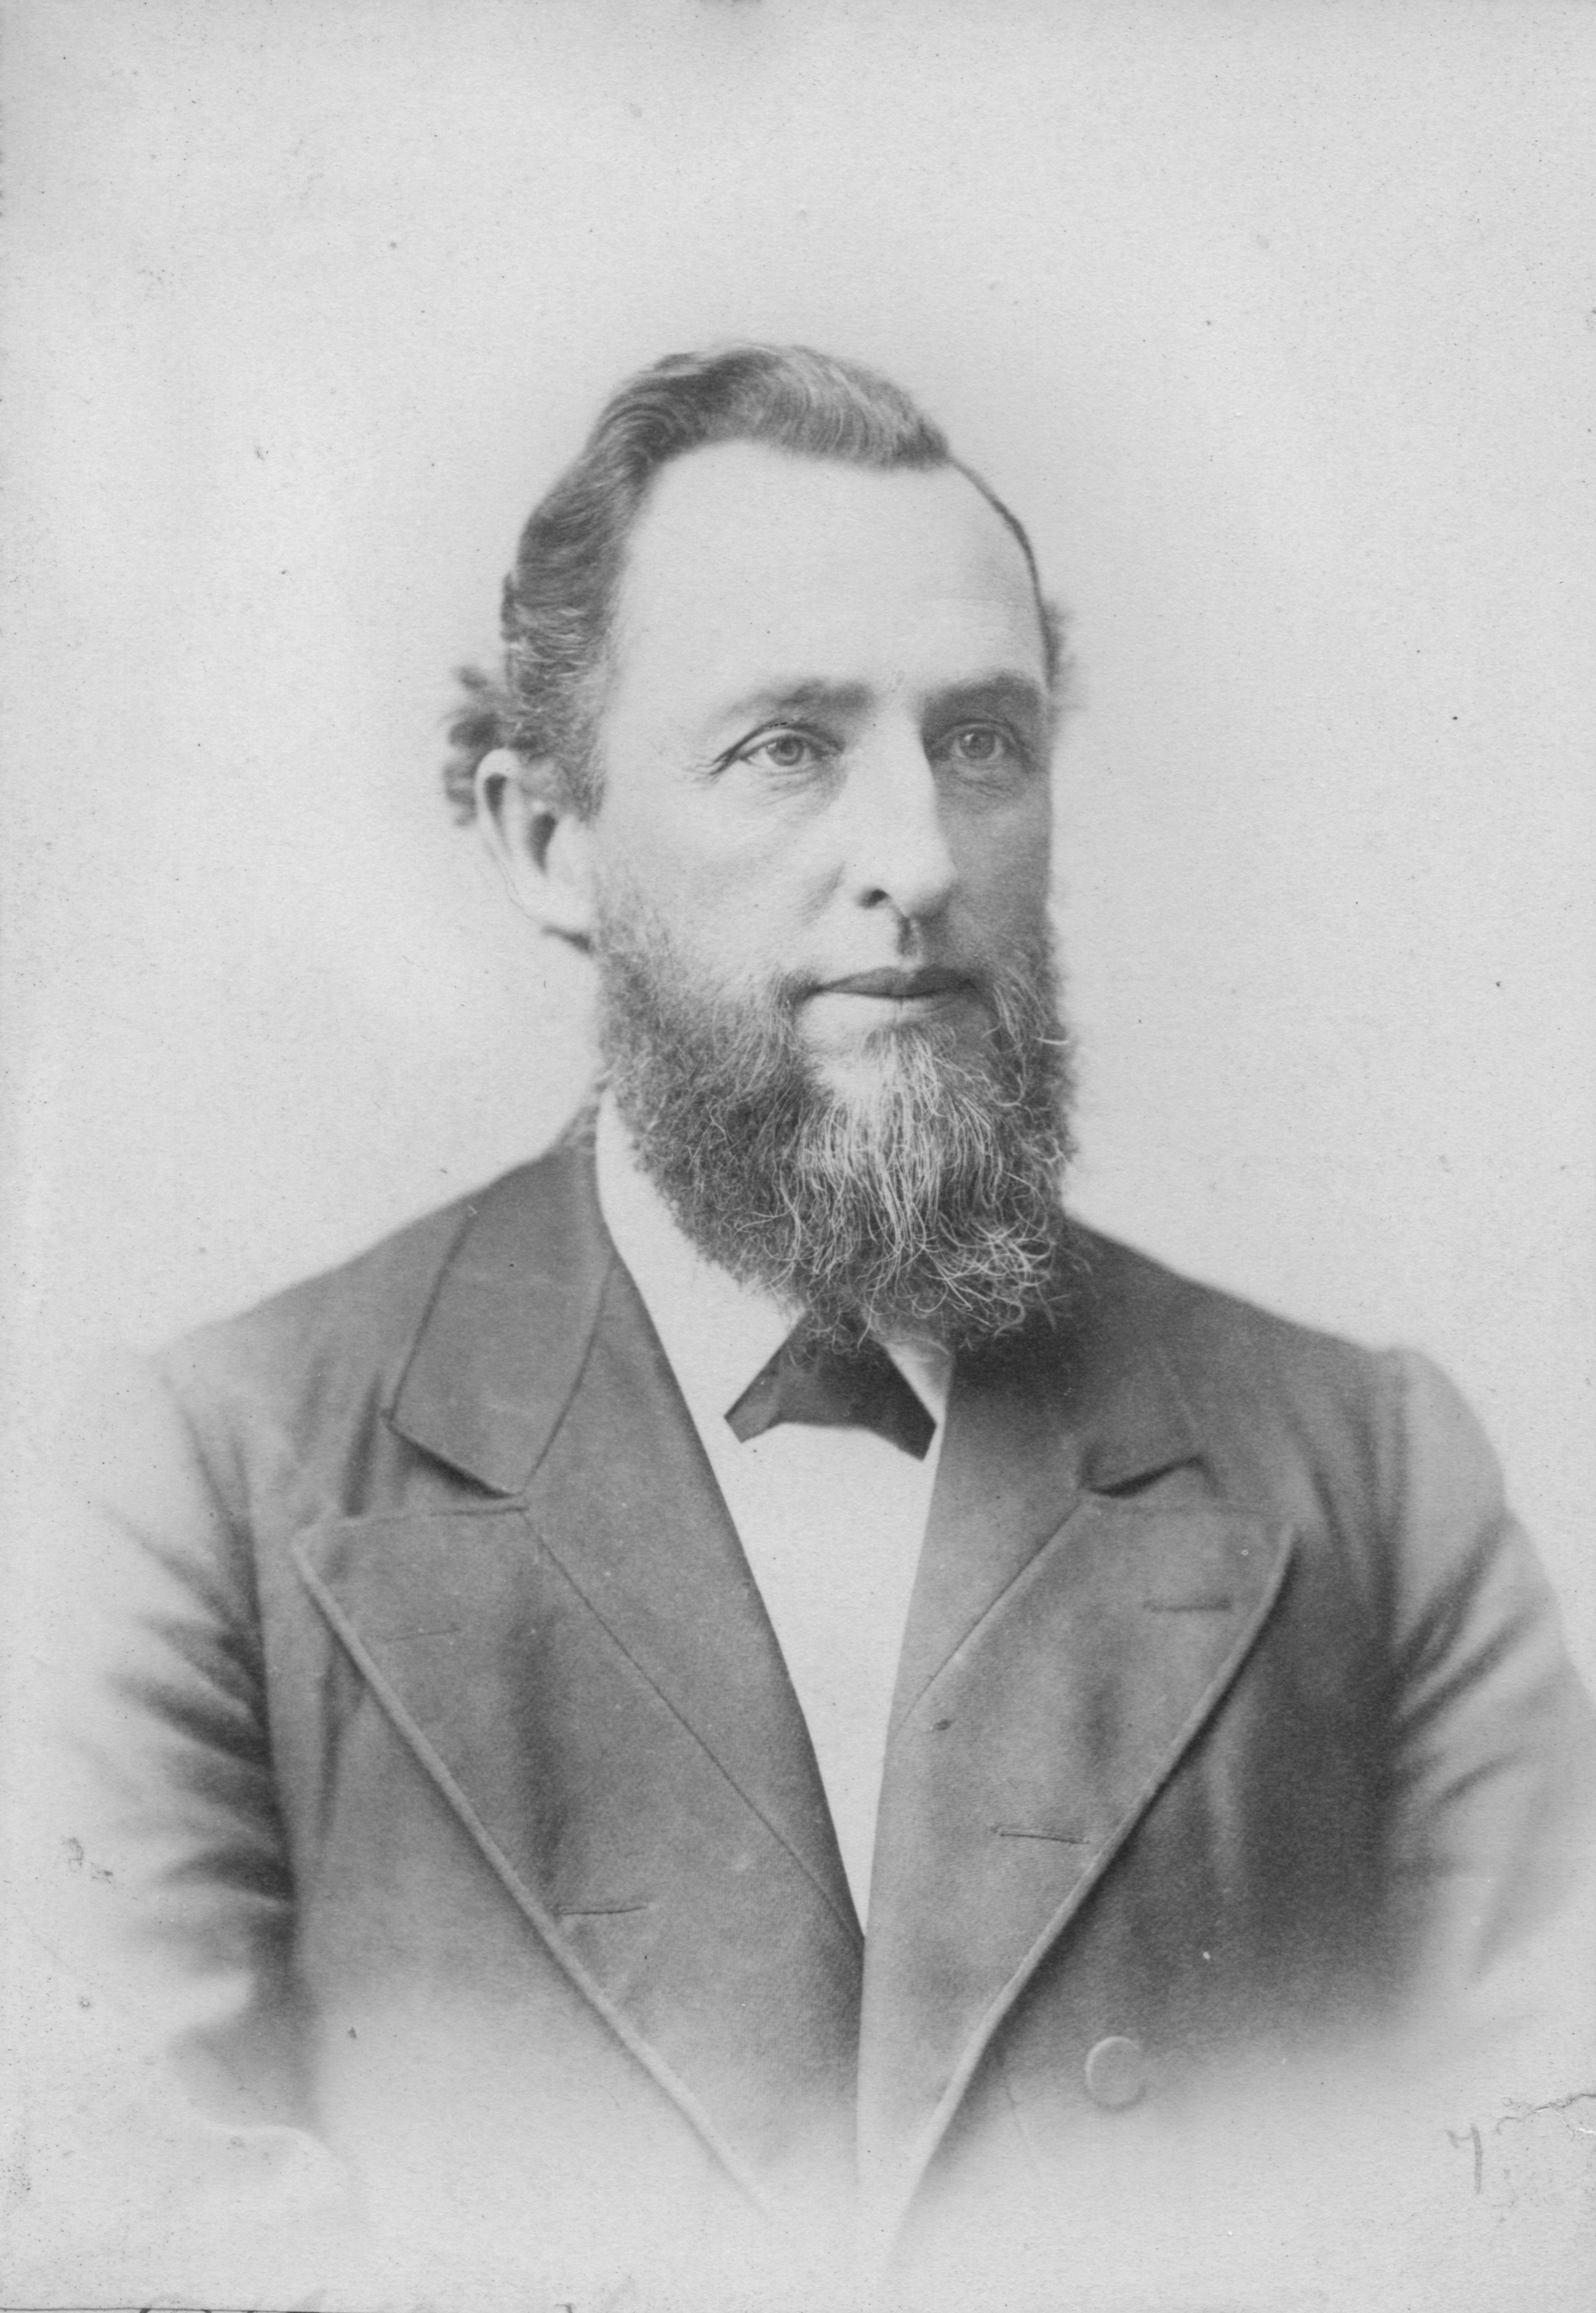
\includegraphics[width=1\linewidth]{images/uriah-smith.jpg}
    \caption*{Uriah Smith (1832-1903)}
    \label{fig:uriah-smith}
\end{figure}


\others{\textbf{Aniołowie są rzeczywistymi istotami}. Są opisani w Biblii jako \textbf{posiadający m.in. twarz, stopy, skrzydła}. Ezechiel mówi o cherubinach: «\textbf{Całe ich \underline{ciało}, ich plecy, ich ręce i ich skrzydła}... Ez 10:12. Aniołowie \textbf{ukazali się} Abrahamowi. Rdz 18:1--8. Rozmawiali i jedli z nim. Poszli do Sodomy i rozmawiali z Lotem, który wszedłszy do swego domu, upiekł dla nich przaśny chleb, a oni jedli. \textbf{Te osoby były nazywane aniołami}. Dawid mówi o mannie jako o zbożu z Nieba i pokarmie aniołów. Ps 78:23--25.}

\othersnogap{Przypadek Balaama, Lb 22:22--31, jest interesującym zdarzeniem. Anioł \textbf{ukazał się} Balaamowi z \textbf{wyciągniętym mieczem w ręku}. Czasami zadawane jest pytanie, \textbf{jak aniołowie mogą być \underline{materialnymi istotami, skoro nie możemy ich zobaczyć}. Ten przypadek to ilustruje}. Zapis mówi, że \textbf{Pan otworzył oczy Balaama i zobaczył on anioła}. \textbf{Anioł nie stworzył ciała na tę okazję}. \textbf{Był dokładnie taki sam jak przed tym, gdy Balaam go zobaczył; \underline{ale zmiana zaszła w Balaamie}}. Jego oczy zostały otwarte i wtedy ujrzał anioła. Tak samo było ze sługą Elizeusza, gdy on i jego pan znaleźli się w trudnym położeniu, otoczeni przez armię króla Syrii. 2Krl 6:17. Elizeusz modlił się, aby \textbf{oczy jego sługi zostały otwarte}; i natychmiast zobaczył on całą górę pełną koni i rydwanów wokół Elizeusza.}

\othersnogap{\textbf{Można to dalej zilustrować odnosząc się do rzeczy, o których wiemy, że są materialne, a jednak których nie możemy zobaczyć}. Powietrze jest materialne, światło jest materialne, nawet myśl sama w sobie jest tylko wynikiem materialnych reakcji — materią działająca na materię — a jednak nie możemy zobaczyć żadnej z tych rzeczy. \textbf{Tak samo jest z aniołami}.}

\othersnogap{\textbf{Dalszym zarzutem wobec materialności aniołów jest to, że są nazywani duchami}. Hbr 1:13--14. \textbf{\underline{Lecz to nie jest zarzut przeciwko temu, że są dosłownymi istotami}}. \textbf{Są po prostu duchowymi istotami skonstruowanymi inaczej niż te ziemskie ciała, które posiadamy}. Paweł mówi, 1Kor 15:44: «\textbf{Jest ciało cielesne i jest \underline{ciało duchowe}}». \textbf{Ciało cielesne mamy teraz; ciało duchowe będziemy mieli przy zmartwychwstaniu}. «\textbf{Jest wskrzeszane jako ciało duchowe}». Werset 44. \textbf{Wtedy będziemy równi aniołom}, Łk 20:36; \textbf{wtedy będziemy mieli ciała podobne do najchwalebniejszego ciała Chrystusa}, Flp 3:4, \textbf{a Chrystus nie jest mniej duchem niż aniołowie}. \textbf{Czytamy, że Bóg jest duchem, to znaczy po prostu \underline{duchową istotą}}.}[James White and Uriah Smith, The Biblical Institute (Kindle Locations 2537-2553). Kindle Edition.]

Biblia daje nam wgląd w to, że aniołowie są duchowymi istotami, które posiadają materialne ciała, ale są dla nas niewidzialni, chyba że Pan otworzy nasze oczy, abyśmy ich zobaczyli. Kiedy sprawiedliwi powstaną w swoich nowych uwielbionych ciałach, powstaną w ciele duchowym, niezniszczalnym. To ciało będzie namacalne i materialne, tak jak nowa ziemia będzie namacalna i materialna. A w naszych duchowych ciałach posiądziemy odnowioną ziemię, będziemy ją \bible{napełniać i czynić ją sobie poddaną; i panować nad rybami morskimi i nad ptactwem niebieskim, i nad wszelką żywą istotą, która porusza się po ziemi}[Rdz 1:28].

% Rzeczywistość nieba

\begin{titledpoem}
    \stanza{
        Bóg nie jest tajemnicą, lecz Istotą prawdziwą, \\
        Na tronie nieba siedzi z chwałą niewątpliwą. \\
        Choć w jednym miejscu przebywa jako Osoba, \\
        Przez Ducha jest obecny, gdzie tylko potrzeba.
    }

    \stanza{
        Duchowa Istota z ciałem i kształtem, \\
        Nie bezcielesny duch, lecz Byt z majestatem. \\
        Syn jest Jego obrazem, tę samą ma naturę, \\
        Obaj są namacalni, to prawda, nie złudzenie.
    }

    \stanza{
        Aniołowie, jak Bóg, są istotami realnymi, \\
        Choć dla oczu śmiertelnych pozostają niewidzialnymi. \\
        Mają ciała duchowe, lecz materialne zarazem, \\
        Takie, jakie my otrzymamy zmartwychwstania obrazem.
    }
\end{titledpoem}

\begin{titledpoem}
    \stanza{
        Niebiańska rzeczywistość nie jest mgłą tajemną, \\
        Lecz światem namacalnym z chwałą niepojemną. \\
        Bóg jako Osoba ma ciało i części, \\
        W jednym miejscu przebywa, lecz Duchem się mieści.
    }

    \stanza{
        Pionierzy adwentyzmu prawdę tę głosili, \\
        Że Bóg i Syn są Istotami, nie duchem bez siły. \\
        Duch Święty to przedstawiciel, nie trzecia Istota, \\
        To przez Niego Bóg działa, gdy pomoc jest potrzebna.
    }

    \stanza{
        Gdy zmartwychwstaniemy w ciałach duchowych, \\
        Będziemy jak aniołowie w kształtach gotowych. \\
        Materialni, namacalni, choć duchowej natury, \\
        Zamieszkamy na ziemi nowej, bez śmierci ponurej.
    }
\end{titledpoem}

\begin{titledpoem}
    \stanza{
        Bóg jest Istotą, nie abstrakcyjną mocą, \\
        Ma kształt i formę, nie jest bezcielesną nocą. \\
        Osobowość Jego to stan bycia Osobą, \\
        Ograniczoną miejscem, lecz z Ducha swobodą.
    }

    \stanza{
        Oczy Balaama ujrzały anioła dopiero, \\
        Gdy Pan je otworzył na prawdę i szczerość. \\
        Tak samo my ujrzymy niebiańskie istoty, \\
        Gdy Bóg nam pozwoli przeniknąć zasłony.
    }

    \stanza{
        Ciało duchowe to nie duch bez ciała, \\
        Lecz byt materialny, którego moc trwała. \\
        W takich ciałach będziemy na nowej ziemi żyli, \\
        Namacalnej, realnej, gdzie Boga będziemy czcili.
    }
\end{titledpoem}
          % Chapter 12
\qrchapter{https://forgottenpillar.com/rsc/pl-fp-chapter13}{Bóg szabatu a Bóg niedzieli — J. B. Frisbie}

Istnieją inne artykuły na temat \emcap{osobowości Boga} napisane przez naszych pionierów i trudno byłoby zawrzeć tu wszystkie, ale chcielibyśmy dodać jeszcze jedno świadectwo z artykułu brata J. B. Frisbie’go, w którym porównuje on Boga szabatu z Bogiem niedzieli. Porównuje on prawdę o \emcap{osobowości Boga} wyrażoną w pierwszym punkcie \emcap{Fundamentalnych Zasad} z doktryną o Trójcy. Przyjrzyjmy się fragmentowi jego artykułu „\textit{Szabat dnia siódmego nie zniesiony}” z \textit{Review and Herald} z 7 marca 1854 roku.

\begin{figure}[hp]
    \centering
    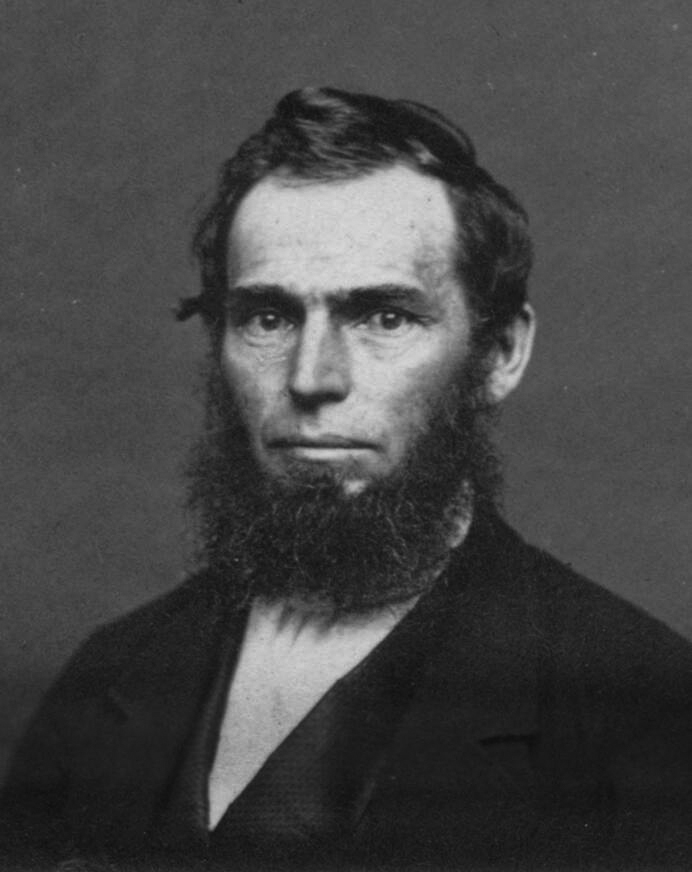
\includegraphics[width=1\linewidth]{images/j-b-frisbie.jpg}
    \caption*{John Byington Frisbie (1816-1882)}
    \label{fig:j-b-frisbie}
\end{figure}


\section*{Bóg szabatu}

\others{Gdy poznamy Boga i będziemy o Nim pamiętać, przestrzegając Jego świętego szabatu, \textbf{wtedy Biblia nauczy nas o Jego osobowości i miejscu zamieszkania}. \textbf{Człowiek jest na obraz i podobieństwo Boga}. Rdz 1:26. «I rzekł Bóg: Uczyńmy (mówiąc do swojego syna) człowieka na nasz obraz, według naszego podobieństwa». Rozdz. 2:7. «I ukształtował Pan Bóg człowieka z prochu ziemi, i tchnął w jego nozdrza tchnienie życia. I stał się człowiek duszą żyjącą». Rdz 9:6; 1Kor 11:7; Jk 3:9. \textbf{To, co zostało stworzone na \underline{obraz i podobieństwo Boga}, zostało uczynione z prochu ziemi i nazwane człowiekiem}.}

\othersnogap{To jest uznawane za prawdziwe znaczenie na podstawie innych świadectw, które można znaleźć w Biblii. \textbf{Jezus był w postaci człowieka i dokładnym obrazem osoby swojego Ojca}.}

\othersnogap{Flp 2:6--8. \textbf{Chrystus Jezus}: «Który, będąc w \textbf{postaci Boga}, nie uważał za grabież być \textbf{równym Bogu}. Lecz ogołocił samego siebie i przyjął \textbf{postać sługi}, i \textbf{został uczyniony na podobieństwo ludzi}». 2Kor 4:4. \textbf{«A będąc ukształtowany na wzór człowieka»}... Kol 1:15. «\textbf{Który jest obrazem niewidzialnego Boga}».}

\othersnogap{Hbr 1:3. \textbf{Syn; «Który, będąc jasnością jego chwały i dokładnym obrazem jego osoby»}. W tym sensie Jezus mógł zgodnie z prawdą powiedzieć do Filipa: «Kto mnie widział, widział i Ojca». J 14:9. Niektórzy wydają się sądzić, że \textbf{przeczy to osobowości Boga, \underline{ponieważ jest On Duchem, i mówią, że nie ma On ciała ani części ciała}}. J 4:24. «\textbf{Bóg jest duchem}». Hbr 1:7. «\textbf{Który czyni swoich aniołów duchami}». \textbf{Kto ośmieliłby się twierdzić, że aniołowie nie mają ciał ani części ciała, ponieważ są duchami}? \textbf{\underline{Niemniej jednak Bóg jest istotą duchową posiadającą ciało i części ciała, o czym dowiadujemy się przez to, że ma miejsce zamieszkania, i ponieważ można go zobaczyć}}. Wj 33:23. «I odejmę moją rękę, i \textbf{ujrzysz moje plecy}, ale \textbf{moje oblicze nie będzie widziane}». Mt 5:8. «Błogosławieni czystego serca, albowiem \textbf{oni zobaczą Boga}». Hbr 12:14. «Dążcie do pokoju ze wszystkimi i do świętości, bez której \textbf{nikt nie ujrzy Pana}». Mt 18:10. «Że w niebie ich aniołowie \textbf{zawsze patrzą na oblicze mojego Ojca, który jest w niebie}». Mt 6:9. «Wy więc tak się módlcie: \textbf{Ojcze nasz, który jesteś w niebie}»... J 6:38. «Bo \textbf{zstąpiłem z nieba} nie po to, żeby czynić swoją wolę, lecz wolę tego, który mnie posłał». Rozdz. 16:28. «\textbf{Wyszedłem od Ojca i przyszedłem na świat}; znowu \textbf{opuszczam świat i idę do Ojca}».}

\othersnogap{\textbf{Czy Bóg nie mówi, że wypełnia nieskończoność przestrzeni? \underline{Odpowiadamy: Nie}}. Ps 139:7, 8. «Dokąd ujdę przed \textbf{twoim duchem}? I dokąd ucieknę przed \textbf{twoją obecnością}? Jeśli wstąpię do nieba, ty tam jesteś»... \textbf{\underline{Bóg przez swojego Ducha może wypełniać niebo i ziemię}}. \textbf{Niektórzy mylą Boga z Jego Duchem, co prowadzi do zamieszania}. Ps 11:4. «\textbf{Pan jest w swoim świętym przybytku, tron Pana jest w niebie}: jego oczy patrzą...». Ha 2:20; Ps 102:19. «Bo spojrzał \textbf{w dół z wysokości swojej świątyni}; \textbf{\underline{z nieba} Pan popatrzył na ziemię»}. 1P 3:12. «Oczy Pana są nad sprawiedliwymi, a jego uszy otwarte są na ich modlitwy...». Ps 80:1. ‘Słuchaj, Pasterzu Izraela, ty, który prowadzisz Józefa jak stado; ty, \textbf{który mieszkasz między cherubinami}, zajaśniej». Ps 99:1; Iz 37:16.}

\othersnogap{J 14:2. «W domu mego Ojca jest wiele posiadłości. Idę przygotować miejsce dla was». Obj 21:2--5; Hbr 11:6. «Bo kto przychodzi do Boga, musi wierzyć, że on jest...». \textbf{To świadectwo uważamy za niezwykle ważne w tym czasie, ażeby wiedzieć, iż jest Bóg. Nie mamy wątpliwości, że gdyby nasze oczy mogły zostać otwarte w wizji lub widzieć tak, jak widzą aniołowie, zobaczylibyśmy Boga w niebie siedzącego na swoim tronie, i jest On obecny we wszystkim, co istnieje, bez względu na to, jak daleko od Niego w Jego stworzeniu}.}[\href{https://documents.adventistarchives.org/Periodicals/RH/RH18540307-V05-07.pdf}{Adventist Review and Sabbath Herald, 7 marca 1854}, J. B. Frisbie, “The Seventh-Day Sabbath Not Abolished”, str. 50]

Tutaj widzimy ten sam argument i rozumowanie, że Bóg jest osobową istotą duchową. Ten Bóg jest Bogiem szabatu. Brat Frisbie porównuje tego Boga z Bogiem niedzieli, który jest Bogiem trynitarnym.

\section*{Bóg niedzieli}

\others{Przedstawimy kilka fragmentów, aby czytelnik mógł \textbf{zobaczyć wyraźny kontrast między \underline{Bogiem Biblii} ujawnionym na światło przez zachowywanie szabatu, a bogiem w ciemności przez zachowywanie niedzieli}. Skrócona wersja katechizmu Kościoła katolickiego autorstwa Wielebnego Johna Dubois, Biskupa Nowego Jorku. Strona 5. «\textbf{Pyt. Gdzie jest Bóg? Odp. Bóg jest wszędzie}. P. Czy Bóg widzi i wie wszystko? O. Tak, On wie i widzi wszystko. \textbf{P. Czy Bóg ma ciało? O. \underline{Nie; Bóg nie ma ciała, jest jedynie Duchem}}. \textbf{P. Czy jest więcej Bogów niż jeden? O. Nie; jest tylko jeden Bóg. P. Czy jest więcej osób niż jedna w Bogu? O. \underline{Tak; w Bogu są trzy osoby}. P. Które to są? O. Bóg Ojciec, Bóg Syn i Bóg Duch Święty. P. Czy nie ma trzech Bogów? O. Nie; Ojciec, Syn i Duch Święty to wszystko jeden i ten sam Bóg}».}

\othersnogap{Pierwszy artykuł Religii Metodystycznej, str. 8. \textbf{«Jest tylko jeden żywy i prawdziwy Bóg}, wieczny, \textbf{bez ciała i części ciała}, o nieskończonej mocy, mądrości i dobroci: stwórca i zachowawca wszystkich rzeczy, widzialnych i niewidzialnych. \textbf{A w jedności tego Bóstwa są trzy osoby jednej substancji, mocy i wieczności; Ojciec, Syn i Duch Święty}.’}

\othersnogap{W tym artykule, podobnie jak w doktrynie katolickiej, \textbf{uczy się nas, że są trzy osoby jednej substancji}, mocy i wieczności tworzące \textbf{w sumie jednego żywego i prawdziwego Boga}, wiecznego \textbf{bez ciała i części ciała}. Ale w tym wszystkim nie powiedziano nam, \textbf{co stało się z ciałem Jezusa, który miał ciało, gdy wstąpił do nieba, który poszedł do Boga, który ‘jest wszędzie» albo nigdzie}. Doksologia.}

\othersnogap{«\textbf{Bogu Ojcu, Bogu Synowi,}} \\
\others{\textbf{Trzem w jednym i Bogu Duchowi}».} \\
\others{Znowu} \\
\others{«Grzeje w słońcu, orzeźwia w powiewie,} \\
\others{Świeci w gwiazdach i kwitnie na drzewie.} \\
\others{\textbf{Wypełnia wszelkie życie, bezkres obejmuje},} \\
\others{Niesie się niepodzielnie i się nie wyczerpuje». — Papież.}

\othersnogap{Te idee dobrze współgrają z poglądami filozofów pogańskich. Jeden mówi, «że woda była podstawą wszystkich rzeczy, a Bóg jest tą duchową istotą, przez którą wszystkie rzeczy są kształtowane z wody». Inny, «że powietrze jest Bogiem, że jest wytwarzane, że jest niezmierzone i nieskończone...». Trzeci, «że Bóg jest duszą przenikającą wszystkie byty natury...». \textbf{Niektórzy wyznają ideę \underline{wyłącznie Ducha}}. I wreszcie, «że Bóg jest wieczną substancją».}

\othersnogap{Te fragmenty są wzięte z \textit{The Ancient History} autorstwa Rollina, tom II, str. 597--598, wydanej przez Harpers. \textbf{Nie powinniśmy raczej wierzyć, że bóg niedzieli pochodzi z tego samego źródła co zachowywanie niedzieli}. «Niedziela (Sunday) była nazwą nadaną przez pogan pierwszemu dniowi tygodnia, ponieważ był to dzień, w którym czcili słońce (the sun)». — The Union Bible Dictionary. \textbf{Później została zmodyfikowana przez Kościół rzymskokatolicki do postaci, w jakiej obecnie jest nauczana w całym kraju}.}

\othersnogap{Bardzo naturalne jest przypuszczenie, że gdy \textbf{Papież ustanowił się Bogiem w świątyni Bożej} [2Tes 2:4], musiał mieć dzień poświęcony dla swojej czci. To właśnie uczynił. — Douay, Katechizm, str. 59. «P. Jaki jest najlepszy sposób na uświęcenie niedzieli? O. Między innymi przez słuchanie mszy. To odprawianie mszy polega na tym, że ksiądz mamrocze po łacinie, pije wino i daje ludziom opłatek do zjedzenia».} \others{Ale Bóg uświęcił swój dzień, ponieważ w nim odpoczął. Inny dzień do zupełnie innego celu. Rdz 2:3.}

\othersnogap{W dniach przed moralnym upadkiem Babilonu Bóg zwracał umysły swoich szczerych dzieci we właściwym kierunku w ich modlitwach, bez względu na to, co mogłyby myśleć w innych chwilach, ale teraz od czasu odstępstwa umysł nie dociera do żadnego boga, tylko do ludzi, jest wiele modlitw do ludzi, które rozpoznajemy po ich wpływie i elokwencji. \textbf{Jesteśmy prawdziwie wdzięczni naszemu niebiańskiemu Ojcu, że \underline{wyprowadził nasze umysły z takiego szaleństwa}, abyśmy poznali i pamiętali \underline{Jego święte imię} przez zachowywanie Jego świętego dnia, abyśmy mogli Go kochać, służyć Mu i godnie \underline{Go chwalić przez naszego wielkiego Arcykapłana w niebiańskiej Świątyni w tym dniu pojednania}}.}[Tamże.][https://documents.adventistarchives.org/Periodicals/RH/RH18540307-V05-07.pdf]

Zanim został adwentystą dnia siódmego, Frisbie był kaznodzieją metodystycznym i zagorzałym przeciwnikiem wierzeń adwentystycznych. W 1853 roku, po debacie na temat szabatu z Josephem Batesem, zmienił swoje stanowisko i zaczął zachowywać szabat oraz głosić doktrynę Adwentystów Dnia Siódmego. Wyrzekł się niedzieli, Trójcy i przyjął prawdę o szabacie dnia siódmego oraz prawdę o Bogu, której Adwentyści Dnia Siódmego nauczali w pierwszym punkcie \emcap{Fundamentalnych Zasad}.

Czy inni pionierzy adwentyzmu dostrzegają niezgodność między doktryną o Trójcy a \emcap{osobowością Boga} wyrażoną w pierwszym punkcie \emcap{Fundamentalnych Zasad}?

% Bóg szabatu a Bóg niedzieli - J. B. Frisbie

\begin{titledpoem}

    \stanza{
        Dwa obrazy Boga, dwie różne natury, \\
        Jeden prawdą jaśnieje, drugi w cieniu bury. \\
        Bóg szabatu osobą z ciałem i częściami, \\
        Bóg niedzieli bezkształtny, rozlany nad światami.
    }

    \stanza{
        Na obraz Stwórcy człowiek uformowany, \\
        Z prochu ziemi przez Boga mądrze ukształtowany. \\
        Syn jest obrazem Ojca, doskonałym odbiciem, \\
        Kto widział Syna, Ojca ujrzał z zachwytem.
    }

    \stanza{
        Bóg ma tron w niebie, miejsce przebywania, \\
        Przez Ducha swego wszędzie jest od zarania. \\
        Nie jest On wszędzie obecny w swej istocie, \\
        Lecz przez Ducha działa w każdej życia dobrocie.
    }

\end{titledpoem}

\begin{titledpoem}

    \stanza{
        Szabat czy niedziela – więcej niż dzień tygodnia, \\
        To wyznanie wiary, co duszę rozpogadnia. \\
        Szabat wskazuje na Boga osobowego, \\
        Niedziela na bóstwo z pogaństwa wyjętego.
    }

    \stanza{
        Bóg szabatu ma ciało, ma oblicze swoje, \\
        Syn Jego jest obrazem, nie jakąś częścią troje. \\
        Bóg niedzieli to "trzech w jednym" bez ciała, \\
        Doktryna, którą filozofia pogańska znała.
    }

    \stanza{
        Jeden Bóg prawdziwy na tronie zasiada, \\
        Drugi wszędzie i nigdzie, jak mgła się rozkłada. \\
        Wybór dnia świętego to wybór Boga twego, \\
        Kogo czcisz naprawdę? Osobę czy coś mglistego?
    }

\end{titledpoem}

\begin{titledpoem}

    \stanza{
        Frisbie odkrył prawdę, gdy szabat przyjmował, \\
        Od metodystów odszedł, Trójcę odrzutował. \\
        Poznał Boga Biblii, nie boga tradycji, \\
        Znalazł prawdę czystą, bez ludzkiej kompozycji.
    }

    \stanza{
        Bóg ma ciało duchowe, ma swoje mieszkanie, \\
        Przez Syna objawia swoje panowanie. \\
        Nie jest On substancją bez formy i kształtu, \\
        Lecz Osobą, co godna czci i zachwytu.
    }

    \stanza{
        Dzień siódmy czy pierwszy – to nie tylko data, \\
        To wyznanie, kogo dusza twa uważa za Brata. \\
        Boga, który stworzył i odpoczął potem, \\
        Czy bóstwo wymyślone ludzkim umysłem i słowem.
    }
    
\end{titledpoem}
          % Chapter 13
\qrchapter{https://forgottenpillar.com/rsc/en-fp-chapter14}{Pionierzy adwentyzmu i doktryna o Trójcy}

Siostra White napisała, że wczesni pionierzy adwentyzmu \egwinline{mają składać swoje świadectwo o tym, co stanowi prawdę na obecny czas}[Lt329-1905.18; 1905][https://egwwritings.org/read?panels=p8455.24], ponieważ \egwinline{nauczyli się unikać błędów i niebezpieczeństw, i czy nie są zatem kompetentni, by udzielać mądrych rad}[7T 287.3; 1902][https://egwwritings.org/read?panels=p117.1637]? W ich pismach widzimy ich jednomyślne poglądy dotyczące \emcap{osobowości Boga} i to, że uniknęli trynitarnego błędu. Jest wiele do napisania na ten temat, ponieważ pionierzy adwentyzmu pozostawili dużo materiału odnoszącego się bezpośrednio lub pośrednio do doktryny o Trójcy. Przyjrzymy się jednak niektórym świadectwom Jamesa White'a i brata Loughborougha, ponieważ przeczytaliśmy niektóre z ich artykułów o \emcap{osobowości Boga}. Porównamy również ich świadectwo z Duchem Proroctwa, jak robiliśmy to do tej pory.

James White wymienił w \textit{Review and Herald} \others{niektóre z \textbf{popularnych baśni} tego wieku}, mówiąc: \others{Tutaj moglibyśmy wspomnieć o \textbf{Trójcy, która \underline{pozbywa się osobowości Boga i Jego Syna Jezusa Chrystusa,}} oraz o pokrapianiu lub polewaniu zamiast bycia «pogrzebanym z Chrystusem w chrzcie», «wszczepionym w podobieństwo Jego śmierci»; ale zostawiamy te \textbf{baśnie}, aż zauważymy jedną, która jest uznawana za świętą przez prawie wszystkich mieniących się chrześcijanami, zarówno katolików jak i protestantów. Jest to zmiana szabatu z czwartego przykazania z siódmego na pierwszy dzień tygodnia.}[James S. White, Review \& Herald, 11 grudnia 1855, str. 85.15][http://documents.adventistarchives.org/Periodicals/RH/RH18551211-V07-11.pdf]

Co James White ma na myśli, gdy mówi, że Trójca \others{pozbywa się osobowości Boga i Jego Syna Jezusa Chrystusa}? W \textit{The Day-Star} napisał:

\others{...pewna klasa, która \textbf{wypiera się jedynego Pana Boga i naszego Pana Jezusa Chrystusa}. Ta klasa nie może być nikim innym jak tymi, którzy \textbf{odrealniają istnienie Ojca i Syna} \textbf{jako \underline{dwóch odrębnych}, \underline{dosłownych}, \underline{namacalnych osób}}, a także dosłownego świętego miasta i tronu Dawida... Sposób, w jaki spirytualiści tak pozbyli się lub \textbf{wyparli jedynego Pana Boga i naszego Pana Jezusa Chrystusa, to po pierwsze przez używanie \underline{starego niebiblijnego trynitarnego wyznania wiary}}, a mianowicie, że Jezus Chrystus jest wiecznym Bogiem, chociaż nie mają ani jednego fragmentu, który by to potwierdzał, podczas gdy nie brakuje nam wyraźnego świadectwo Pisma, \textbf{że jest On Synem wiecznego Boga.}}[James White, The Day-Star, 24 stycznia 1846.][https://m.egwwritings.org/en/book/741.25\#27]

Pozbywanie się osobowości Boga i Jego Syna dokonuje się poprzez wyparcie się Ich jako dwóch odrębnych, dosłownych i namacalnych osób. Doktryna o osobowości Boga naucza, że Ojciec ma dosłowną, \textit{namacalną} osobę.

W artykule z \textit{Adventist Review and Sabbath Herald} z 4 kwietnia 1854 roku James White wymienił 10 punktów dotyczących „\textit{katolickich powodów zachowywania niedzieli}”, gdzie powiedział, że niedziela “\others{jest dniem poświęconym przez apostołów \textbf{ku czci Trójcy Przenajświętszej}}[The Advent Review, and Sabbath Herald, tom 5, 4 kwietnia 1854, str. 86.][https://egwwritings.org/read?panels=p1643.2867]. Tutaj również widzimy zgodę między J. B. Frisbie a Jamesem White'em w ich poglądzie, że szabat jest poświęcony biblijnemu Bogu wyrażonemu w pierwszym punkcie \emcap{Fundamentalnych Zasad}, a niedziela jest poświęcona trynitarnemu Bogu. Głównym problemem z doktryną o Trójcy jest to, że \others{pozbywa się osobowości Boga i Jego Syna Jezusa Chrystusa}. W \textit{Life Incidents} napisał więcej o tym, dlaczego tak jest.

\others{\textbf{Jezus modlił się, aby jego uczniowie byli jedno, tak jak On był \underline{jedno ze swoim Ojcem}}. \textbf{Ta modlitwa nie była o jednym uczniu z dwunastoma głowami, ale o dwunastu uczniach zjednoczonych w celu i wysiłku w sprawie ich Mistrza}. \textbf{\underline{Ani też Ojciec, ani Syn nie są częściami «trójjedynego Boga».}}\footnote{Ten sam cytat znajduje się w książce Jamesa White'a \textit{The Law and the Gospel} z jedną różnicą. Stwierdza on: “\textit{Ani Ojciec, ani Syn nie są częściami \underline{jednej istoty}}”; w \textit{Life Incidents} napisał „częściami «\underline{trój-jedynego Boga}»”. Zobacz \href{https://egwwritings.org/?ref=en_LAGO.1.2&para=1492.10}{James S. White, The Law and the Gospel str. 1--2}.} \textbf{\underline{Są oni dwoma odrębnymi istotami}}, \textbf{jednak są jedno w zamyśle i dokonaniu odkupienia}. Odkupieni, od pierwszego, który uczestniczy w wielkim odkupieniu, do ostatniego, wszyscy przypisują cześć, chwałę i uwielbienie za swoje zbawienie \textbf{zarówno Bogu, jak i Barankowi}.}[James S. White, Life Incidents, str.343.2][https://egwwritings.org/read?panels=p1462.1743]

Siostra White napisała podobnie na temat modlitwy Chrystusa:

\egw{Brzemieniem tej modlitwy było to, aby Jego uczniowie byli \textbf{jedno, tak jak On był jedno z Ojcem}; jedność tak bliska, że \textbf{chociaż byli \underline{dwiema odrębnymi istotami}}, istniała \textbf{doskonała jedność ducha, celu i działania}. Umysł Ojca był umysłem Syna}[Lt1-1882.1; 1882][https://egwwritings.org/read?panels=p4120.5]

\egw{\textbf{Jedność, która istnieje między Chrystusem a Jego uczniami, \underline{nie niszczy osobowości żadnej ze stron}}. Są jednością w celu, w umyśle, w charakterze, \textbf{ale \underline{nie w osobie}}. \textbf{W ten sposób Bóg i Chrystus są jednością}}[MH, 421 422; 1905][https://egwwritings.org/read?panels=p135.2177]

Ojciec i Syn nie stanowią jednej osoby ani jednej istoty. Ojciec i Syn są jednością, tak jak Chrystus i Jego uczniowie są jednością — jednością w duchu, celu, umyśle i charakterze.

Wielu adwentystycznych trynitarnych uczonych oskarża Jamesa White'a i innych wczesnych pionierów o arianizm lub pół-arianizm, twierdząc, że czynili oni Chrystusa podrzędnym wobec Ojca. To nieprawda. Przeczytajmy świadectwo Jamesa White'a w tej sprawie.

\others{Paweł potwierdza o \textbf{Synu Bożym, że był On w postaci Boga}, i że \textbf{\underline{był równy Bogu}}. «\textbf{Który będąc w postaci Boga, nie uważał za grabież być \underline{równym Bogu}}». Flp 2:6. Powodem, dla którego nie jest grabieżą dla Syna \textbf{być równym Ojcu, jest fakt, że jest równy}. Jeśli Syn nie jest równy Ojcu, wtedy jest grabieżą, gdy stawia się na równi z Ojcem.}

\othersnogap{\textbf{\underline{Niewytłumaczalna trójca, która czyni bóstwo trzema w jednym i jednym w trzech, jest wystarczająco zła}}; \textbf{ale ten skrajny unitarianizm, który czyni Chrystusa podrzędnym wobec Ojca jest gorszy}. Czy Bóg powiedział do kogoś podrzędnego: «Uczyńmy człowieka na nasz obraz?»}[James S. White, The Advent Review and Sabbath Herald, 29 listopada 1877, str. 171][https://documents.adventistarchives.org/Periodicals/RH/RH18771129-V50-22.pdf]

Problem adwentystycznych trynitarnych uczonych polega na tym, że sami nie potrafią w pełni wyjaśnić boskości Chrystusa inaczej niż przez paradygmat trynitarny. Pionierzy adwentystyczni wierzyli w pełną boskość Chrystusa, ale odrzucali Trójcę, ponieważ niszczy ona \emcap{osobowość Boga}. \others{Niewytłumaczalna trójca, która czyni bóstwo trzema w jednym i jednym w trzech, \textbf{jest wystarczająco zła}}. Poniżej znajduje się kolejne oświadczenie Jamesa White'a, w którym porównał wierzenia Adwentystów Dnia Siódmego z wierzeniami Baptystów Dnia Siódmego. Adwentyści Dnia Siódmego nie wierzyli w Trójcę, w przeciwieństwie do Baptystów Dnia Siódmego. James White wspomniał, że w kwestii boskości Chrystusa Adwentyści Dnia Siódmego są tak blisko trynitarnych Baptystów Dnia Siódmego, że nie spodziewają się tam żadnego problemu.

\others{\textbf{Główna różnica między tymi dwoma grupami dotyczy kwestii nieśmiertelności}. \textbf{Adwentyści Dnia Siódmego wyznają \underline{boskość Chrystusa tak blisko trynitarian}, że nie spodziewamy się tu żadnego problemu}. A ponieważ praktyczne zastosowanie tematu Darów Ducha dla naszego ludu i naszej pracy jest lepiej rozumiane przez naszych braci Baptystów Dnia Siódmego, okazują oni mniej troski o nas w tej kwestii.}[James S. White, The Advent Review and Sabbath Herald, 12 października 1876, str. 116][https://documents.adventistarchives.org/Periodicals/RH/RH18761012-V48-15.pdf]

Te dowody powinny wzbudzić pytania u każdego adwentystycznego trynitarnego uczonego. Jak to możliwe, że pionierzy adwentystyczni uznawali boskość Chrystusa tak jak trynitarianie, a jednak odrzucali doktrynę o Trójcy? W jaki sposób Chrystus był w pełni boski, jeśli nie był częścią połączonego trój-jedynego Boga? Odpowiedź jest prosta i całkowicie biblijna. Chrystus jest w pełni boski, tak jak Jego Ojciec, ponieważ został zrodzony na dokładny obraz osoby Ojca; w ten sposób odziedziczył kompletną boską naturę od swojego Ojca.

\egw{Została złożona kompletna ofiara; gdyż «tak Bóg umiłował świat, że dał swego jednorodzonego Syna» —\textbf{nie syna przez stworzenie}, jak aniołowie, ani syna przez adopcję, jak grzesznik, któremu przebaczono, ale \textbf{Syna \underline{zrodzonego} na dokładny obraz osoby Ojca}, i w całej jasności Jego majestatu i chwały, \textbf{równego Bogu} w autorytecie, godności i \textbf{boskiej doskonałości}. \textbf{W Nim zamieszkała cała pełnia Bóstwa cieleśnie}.}[ST May 30, 1895, par. 3; 1895][https://egwwritings.org/read?panels=p820.12891]

Pełna boskość Chrystusa nie opiera się na połączonej \emcap{osobowości Boga}, ale raczej na Jego synostwie względem Ojca. Biblia nigdy nie odnosi się do Chrystusa za pomocą terminu „\textit{jeden Bóg}” — tylko Ojciec jest określany terminem „\textit{jeden Bóg}”\footnote{J 17:3; 1Kor 8:6; 1Tm 2:5; Ef 4:6} \footnote{Badamy pełną boskość Chrystusa dogłębnie w drugiej książce projektu Forgotten Pillar — \textit{Odkrywając Filar na nowo}.}. Jezus, Syn Boży, jest w pełni boski, ale nie jest określany jako \others{\textbf{jeden Bóg}, \textbf{osobowa, duchowa istota}} w pierwszym punkcie \emcap{Fundamentalnych Zasad}.

\egw{Pan Jezus Chrystus, jednorodzony Syn Ojca, \textbf{jest prawdziwie Bogiem w nieskończoności, \underline{ale nie w osobowości}}}[Ms116-1905.19; 1905][https://egwwritings.org/read?panels=p10633.25]

Brat J. N. Loughborough został poproszony o odpowiedź na pytanie: \others{Jakie poważne zastrzeżenia istnieją wobec doktryny o Trójcy?}[Pytanie zostało zadane przez Brata W. W. Gilesa i zostało przesłane do Jamesa S. White'a, który przekazał je bratu Johnowi N. Loughboroughowi.]. Czytając jego odpowiedź, spróbujmy zrozumieć niektóre z powodów, dla których pierwsi pionierzy nie przyjęli tej doktryny.

\others{Jest wiele zastrzeżeń, które moglibyśmy wysunąć, ale ze względu na ograniczoną przestrzeń skrócimy je do trzech następujących: \textbf{1. Jest sprzeczna ze zdrowym rozsądkiem. 2. Jest sprzeczna z Pismem. 3. Jej pochodzenie jest pogańskie i bajeczne.}}

\othersnogap{Omówimy te stanowiska pokrótce w tej kolejności. Zatem 1. \textbf{Nie jest zgodne ze zdrowym rozsądkiem mówić o trzech jako jednym i jednym jako trzech}. \textbf{Albo, jak niektórzy to wyrażają, nazywając Boga «Trójjedynym Bogiem», czyli «Bogiem trzy-w-jednym».} \textbf{Jeśli Ojciec, Syn i Duch Święty są każdy Bogiem, byłoby trzech Bogów; ponieważ trzy razy jeden to nie jeden, lecz trzy}. \textbf{\underline{Istnieje sens, w którym są jedno, ale nie są jedną osobą, jak twierdzą trynitarianie}}}.

\othersnogap{2. \textbf{Jest sprzeczna z Pismem}. \textbf{Prawie każdy fragment Nowego Testamentu, który mówi o Ojcu i Synu, przedstawia ich jako dwie odrębne osoby}. \textbf{\underline{Sam siedemnasty rozdział Ewangelii Jana wystarczy, aby obalić doktrynę o Trójcy}}. \textbf{Ponad czterdzieści razy w tym jednym rozdziale Chrystus mówi o swoim Ojcu jako o osobie odrębnej od siebie}. Jego Ojciec był w niebie, a On na ziemi. Ojciec Go posłał. Dał Mu tych, którzy uwierzyli. Miał potem pójść do Ojca. \textbf{I w tym właśnie świadectwie pokazuje nam, na czym polega jedność Ojca i Syna}. \textbf{\underline{Jest ona taka sama jak jedność członków Kościoła Chrystusowego}}. «\textbf{Aby \underline{oni} wszyscy byli jedno; \underline{jak} ty, Ojcze, we mnie, a ja w tobie, \underline{aby i oni} byli jedno w nas}; aby świat uwierzył, że ty mnie posłałeś. A \textbf{chwałę, którą mi dałeś, dałem im}; aby \textbf{byli jedno}, \textbf{tak jak my jedno jesteśmy}». \textbf{Jednego serca i jednego umysłu}. \textbf{Jednego celu} w całym planie opracowanym dla zbawienia człowieka. \textbf{\underline{Przeczytajcie siedemnasty rozdział Ew. Jana i zobaczcie, czy nie obala on całkowicie doktryny o Trójcy}}.}

\othersnogap{\textbf{Aby wierzyć w tę doktrynę, czytając Pismo, musimy uwierzyć, że Bóg posłał samego siebie na świat, umarł, aby pojednać świat z samym sobą, wskrzesił samego siebie z martwych, wstąpił do samego siebie do nieba, wstawia się przed samym sobą w niebie, aby pojednać świat z samym sobą i jest jedynym pośrednikiem między człowiekiem a samym sobą}. Nie wystarczy zastąpić ludzką naturę Chrystusa (według trynitarian) jako Pośrednika; ponieważ Clarke mówi: «Ludzka krew nie może bardziej przebłagać Boga niż krew świni». Komentarz do 2Sm 21:10. \textbf{Musimy także wierzyć, że w ogrodzie Bóg modlił się do samego siebie, że jeśli to możliwe, aby kielich został oddalony od niego samego, i w tysiąc innych \underline{takich absurdów}}.}

\others{\textbf{Przeczytajcie uważnie następujące teksty, zestawiając je z ideą, że Chrystus jest Wszechmocnym, Wszechobecnym, Najwyższym i jedynym samoistnym Bogiem: J 14:28; 17:3; 3:16; 5:19, 26; 11:15; 20:19; 8:50; 6:38; Mk 13:32; Łk 6:12; 22:69; 24:29; Mt 3:17; 27:46; Ga 3:20; 1J 2:1; Obj 5:7; Dz 17:31. Zobacz także Mt 11:25, 27; Łk 1:32; 22:42; J 3:35, 36; 5:19, 21, 22, 23, 25, 26; 6:40; 8:35, 36; 14:13; 1Kor 15:28 itd.}}

\othersnogap{\textbf{Słowo Trójca nie występuje nigdzie w Piśmie}. \textbf{Główny tekst, który podobno jej naucza, to 1J 1:7\footnote{J. N. Loughborough popełnił literówkę w oryginalnym dokumencie; chciał wskazać na 1J 5:7}, który jest interpolacją}. Clarke mówi: «\textbf{Ze stu trzynastu manuskryptów tekstu tego brakuje w stu dwunastu. Nie występuje w żadnym manuskrypcie przed dziesiątym wiekiem. A pierwsze miejsce, w którym tekst pojawia się po grecku, to greckie tłumaczenie aktów Soboru Laterańskiego, który odbył się w 1215 roku n.e.}». — Komentarz do Ew. Jana 1 i uwagi na końcu rozdziału.}

\othersnogap{3. \textbf{Jej pochodzenie jest pogańskie i bajeczne}. Zamiast wskazywać nam Pismo jako dowód trójcy, wskazuje się nam na trójząb Persów, z twierdzeniem, że przez to chcieli nauczać idei trójcy, a jeśli mieli doktrynę o trójcy, musieli ją otrzymać przez tradycję od ludu Bożego. \textbf{Ale to wszystko jest założeniem, ponieważ jest pewne, że Kościół żydowski nie wyznawał takiej doktryny. Pan Summerbell mówi: «Mój przyjaciel, który był obecny w synagodze w Nowym Jorku, zapytał Rabina o wyjaśnienie \underline{słowa ‘elohim’}. Duchowny trynitarny, który stał obok, odpowiedział: ‘Cóż, to ma \underline{odniesienie do trzech osób w Trójcy}’, gdy Żyd wystąpił naprzód i powiedział, że nie wolno mu więcej wymawiać tego słowa, bo będą musieli zmusić go do opuszczenia budynku; \underline{ponieważ nie było dozwolone wymawianie imienia żadnego obcego boga w synagodze}».}\footnote{Dyskusja między Summerbellem a Floodem o Trójcy, str. 38.} Milman mówi, że idea trójzębu jest bajeczna. (Hist. Christianity, str. 34.)}

\others{\textbf{Ta doktryna o trójcy została wprowadzona do Kościoła mniej więcej w tym samym czasie co oddawanie czci obrazom i zachowywanie dnia słońca, i jest jedynie przerobioną doktryną perską}. \textbf{Od jej wprowadzenia do ukształtowania doktryny w obecnej formie upłynęło około trzystu lat. Rozpoczęło się to około 325 roku n.e., a zakończyło się w 681 roku.} Zobacz Milman's Gibbon's Rome, tom IV, str. 422. Została przyjęta w Hiszpanii w 589 roku, w Anglii w 596 roku, w Afryce w 534 roku - Gib. tom IV, str. 114, 345; Milner, tom I, str. 519.}[John N. Loughborough, The Advent Review, and Sabbath Herald, 5 listopada 1861, str. 184][https://egwwritings.org/read?panels=p1685.6615]

Brat Loughborough był synem pastora metodystycznego i został wychowany w wierze w doktrynę o Trójcy. Poza wymienionymi powodami nie przyjmuje on tej doktryny, ponieważ nie jest ona zgodna z prawdą o \emcap{osobowości Boga}. Siedemnasty rozdział Ew. Jana jest zgodny z prawdą o \emcap{osobowości Boga} nauczaną i praktykowaną przez Adwentystów Dnia Siódmego; doktryna o Trójcy nie jest.

\begin{figure}[hp]
    \centering
    \includegraphics[width=1\linewidth]{images/john-nevins-andrews.jpg}
    \caption*{John Nevins Andrews (1829-1883)}
    \label{fig:j-n-andrews}
\end{figure}

J. N. Andrews powiedział: \others{\textbf{Doktryna o Trójcy, która została ustanowiona w Kościele przez sobór nicejski w 325 roku n.e.} \textbf{Ta doktryna \underline{niszczy osobowość Boga i Jego Syna Jezusa Chrystusa, naszego Pana}}...}[John. N. Andrews, The Advent Review and Sabbath Herald, 6 marca 1855, str. 185][http://documents.adventistarchives.org/Periodicals/RH/RH18550306-V06-24.pdf]

W kontekście trynitarnego rozumienia \emcap{osobowości Boga} można bezpiecznie powiedzieć, że \emcap{osobowość Boga}, czyli właściwość lub stan Boga jako osoby, w każdym rozumieniu doktryny o Trójcy jest tajemnicą. Problem polega na tym, że nie ma jasnego poglądu, kim jest ten \textit{jeden Bóg}, który jest osobą? Podstawowe twierdzenie mówi, że Bóg jest Jeden, ale Trzema, lub Jeden w Trzech; tak, Bóg jest osobą i jest jeden, ale jednocześnie jest trzema osobami. Ten pogląd nigdy nie może mieć jasnego postrzegania \emcap{osobowości Boga}. Ponadto zaprzeczy on najwyraźniejszemu świadectwu Pisma Świętego, że jedynym Bogiem jest Ojciec, a Chrystus jest prawdziwie Jego jednorodzonym Synem. Większość braci trynitarnych zgodziłaby się, że Chrystus jest realną i określoną istotą, ale gdyby trynitarianin miał zaakceptować Ojca jako realną i określoną Istotę, musiałby również zaakceptować Ducha Świętego jako realną i określoną istotę, tym samym zaprzeczając, że Duch Święty jest \textit{duchem}, środkiem, przez który Ojciec i Syn są wszechobecni. I odwrotnie, gdyby trynitarianin zaakceptował Ducha Świętego jako dosłownego ducha, niemającego ciała ani formy, zaprzeczyłby wtedy, że Ojciec jest realną, określoną istotą. W rozmowie o właściwości lub stanie Boga jako osoby nigdy nie ma jasnego poglądu na tę sprawę wśród zwolenników doktryny o Trójcy; to wybieg. \textit{«Wybiegi»} to słowo, którego Siostra White użyła do opisania oszustwa poprzez podstęp lub fortel w celu ukrycia, ucieczki lub uniknięcia\footnote{\href{https://www.merriam-webster.com/dictionary/subterfuges}{The Merriam-Webster, ‘subterfuges’} - “\textit{deception by artifice or stratagem in order to conceal, escape, or evade}”} prawdy; innymi słowy, coś, czego nie można złapać ani za głowę, ani za ogon. To jest główny powód, dla którego siostra White nie angażowała się w dyskusję o Trójcy, która miała się pojawić w Kościele Adwentystów Dnia Siódmego.

\egw{Ostrzeżono mnie, abym nie wchodziła w spór \textbf{dotyczący kwestii}, które \textbf{\underline{pojawią się}} w związku z \textbf{tymi sprawami, ponieważ spór \underline{mógłby doprowadzić ludzi do uciekania się do wybiegów, a ich umysły zostałyby odwiedzione od prawdy Słowa Bożego do przypuszczeń i domysłów}}. \textbf{Im więcej dyskutuje się o fantazyjnych teoriach, tym \underline{mniej ludzie będą wiedzieć o Bogu i o prawdzie, która uświęca duszę}}}[Lt232-1903.41; 1903][https://egwwritings.org/read?panels=p10197.50]

Kiedy czytamy dzieła pionierów Adwentystów Dnia Siódmego na temat \emcap{osobowości Boga}, widzimy, że nie wpadli oni w pułapkę Trójcy. Ich nietrynitarne poglądy na temat Boga nie wynikały z niewiedzy, lecz z poznania prawdy o \emcap{osobowości Boga}. Byli oni ludźmi o bystrym i szlachetnym intelekcie, rozumiejącymi cienką linię między prawdą a błędem. Ich zrozumienie \emcap{osobowości Boga} jest zrównoważone i solidne, mocno wsparte prostym i jasnym „\textit{tak mówi Pan}”.

Wielu adwentystów akceptuje dziś doktrynę o Trójcy, ponieważ Ellen White rzekomo ją zaakceptowała i promowała. Jest to dalekie od prawdy, a taki wniosek wynika z braku znajomości Ducha Proroctwa. Jeśli ktokolwiek był zaznajomiony z wierzeniami siostry White, to był to jej mąż James White. Oto co ma do powiedzenia o pismach swojej żony:

\others{\textbf{Zapraszamy wszystkich do porównania świadectw Ducha Świętego poprzez panią White ze słowem Bożym}. \textbf{I w tym nie zapraszamy was do porównywania ich \underline{z waszym wyznaniem wiary}}. To jest zupełnie co innego. \textbf{\underline{Trynitarianin może porównać je ze swoim wyznaniem wiary i potępić je, ponieważ się z nim nie zgadzają}}. Przestrzegający niedzieli lub człowiek, który uważa wieczne męki za ważną prawdę, i pastor, który kropi niemowlęta, każdy może potępić świadectwa pani White, ponieważ nie zgadzają się z ich szczególnymi poglądami. I setka innych, z których każdy ma inne poglądy, może dojść do tego samego wniosku. \textbf{Jednak ich autentyczność nigdy nie może być sprawdzona w ten sposób}.}[James S. White, The Advent Review, and Herald of the Sabbath, 13 czerwca 1871.][https://documents.adventistarchives.org/Periodicals/RH/RH18710613-V37-26.pdf]

James White był najbliższym współpracownikiem Ellen White, osobą, która była z nią jedno w Bożym budowaniu Kościoła Adwentystów Dnia Siódmego. Mamy jasne i bezpośrednie świadectwo od niego, że pisma Ellen White nie są trynitarne. Dziś uczeni przedstawiają fałszywą narrację, że Ellen White rozwinęła swoje zrozumienie doktryny o Trójcy i ostatecznie ją zaakceptowała i głosiła. Ale widzimy, że Ellen White nie zmieniła swojego stanowiska w sprawie \emcap{osobowości Boga} ani nie przyjęła doktryny o Trójcy. Była jednoznaczna w swoim twierdzeniu, że nigdy tego nie zrobiła. Kiedy nadszedł kryzys Kellogga dotyczący \emcap{osobowości Boga}, pozostała niewzruszona w swoim poglądzie, tak jak wszyscy wcześni pionierzy Adwentystów Dnia Siódmego — a jej postępowanie z dr. Kelloggiem to udowadnia. To prawda, doktryna o Trójcy \textit{nie może być przyjęta przez lojalnych wobec wiary i zasad, które wytrzymały wszelki sprzeciw szatańskich wpływów}.\footnote{\egw{Łatane teorie nie mogą być przyjęte przez lojalnych wobec wiary i zasad, które wytrzymały wszelki sprzeciw szatańskich wpływów}[Lt253-1903.28; 1903][https://egwwritings.org/read?panels=p14068.9980036]} Dzisiejsza oficjalna narracja, że Ellen White nauczała o Trójcy, przypomina twierdzenie dr. Kellogga, że książka \textit{The Living Temple} nauczała tego samego, co Ellen White. \egwinline{\textbf{Ale broń Boże, żeby ten pogląd przeważył}}[SpTB02 53.3; 1904][https://egwwritings.org/read?panels=p417.272]

% Pionierzy adwentyzmu i doktryna o Trójcy

\begin{titledpoem}
    \stanza{
        Pionierzy adwentyzmu prawdę głosili śmiało, \\
        O Bogu i Jego Synu świadectwo trwało. \\
        Odrzucili doktrynę, co Bożą osobowość niszczy, \\
        Trzymając się Pisma w wierze najczystszej.
    }

    \stanza{
        James White nazwał Trójcę "popularną baśnią" wprost, \\
        Która osobowość Boga i Syna usuwa w tłum. \\
        Ojciec i Syn to dwie odrębne istoty, \\
        Nie złączone w jedną, jak uczą trynitarne cnoty.
    }

    \stanza{
        Jedność ich w duchu, celu i działaniu trwa, \\
        Jak uczniów z Chrystusem, choć każdy siebie ma. \\
        Nie w osobie są jednym, lecz w zamiarze swym, \\
        Tak Bóg i Chrystus jednością są w dziele tym.
    }

    \stanza{
        Chrystus w pełni boski, bo z Ojca zrodzony, \\
        Nie przez stworzenie, lecz jako Syn uwielbiony. \\
        Na obraz Ojca dokładny ukształtowany, \\
        W boskiej naturze w pełni uczestniczy oddany.
    }
\end{titledpoem}

% Druga poezja o Trójcy i pionierach adwentyzmu

\begin{titledpoem}
    \stanza{
        Loughborough pytany o Trójcy zastrzeżenia, \\
        Trzy powody podał godne rozważenia. \\
        Sprzeczna ze zdrowym rozsądkiem i z Pismem całym, \\
        Z pogańskich źródeł pochodzi z blaskiem niemałym.
    }

    \stanza{
        Jak może Bóg być trzema i jednym zarazem? \\
        Jak może modlić się do siebie własnym głosem? \\
        Jan siedemnasty rozdział tę doktrynę obala, \\
        Gdy Chrystus o Ojcu jako odrębnym wspomina.
    }

    \stanza{
        Pionierzy widzieli jasno, co Pismo objawia, \\
        Że Ojciec jest Bogiem, a Chrystus Synem zostaje. \\
        Nie przez tajemnicę, lecz przez proste słowa, \\
        Prawda o Bogu w ich pismach się chowa.
    }

    \stanza{
        Ellen White z mężem w jedności trwali, \\
        Tę samą prawdę o Bogu wyznawali. \\
        Nie zmieniła poglądów, jak niektórzy twierdzą, \\
        Lecz wierną pozostała prawdzie z Bożą pieczęcią.
    }
\end{titledpoem}

% Trzecia poezja o osobowości Boga

\begin{titledpoem}
    \stanza{
        Osobowość Boga to filar wiary prawdziwej, \\
        Nie tajemnica w formule trynitarnej fałszywej. \\
        Bóg jest osobą realną, określoną jasno, \\
        Nie abstrakcją, co w trójcy ginie przedwcześnie.
    }

    \stanza{
        Ojciec i Syn w miłości zjednoczeni, \\
        Przez Ducha Świętego w sercach objawieni. \\
        Nie trzy osoby w jednej istocie złączone, \\
        Lecz Ojciec najwyższy i Syn z Niego zrodzony.
    }

    \stanza{
        Pionierzy tę prawdę z Pisma czerpali, \\
        Przed błędem trynitarnym wiernych ostrzegali. \\
        Ich świadectwo jasne jak światło poranka, \\
        Prowadzi do Boga, nie do ludzkiego zamku.
    }

    \stanza{
        Niech prawda o Bogu w sercach rozbrzmiewa, \\
        Jak u pionierów, co wiernie ją wyznawali. \\
        Bez wybiegów, domysłów i ludzkich tradycji, \\
        Lecz w prostocie wiary, co duszę oczyści.
    }
\end{titledpoem}
          % Chapter 14
\chapter{Dr Kellogg i doktryna o Trójcy}

Kluczowym problemem kontrowersji  Kellogga były poglądy dotyczące \emcap{osobowości Boga}, które odchodziły od fundamentu naszej wiary, jakie Bóg ustanowił na początku naszej pracy. Powiedziano nam, że \egwinline{Wiele podobnych rzeczy pojawi się w przyszłości}[Ms137-1903.10; 1903][https://egwwritings.org/?ref=en\_Ms137-1903.10&para=9939.17]. W książce The Living Temple widzimy poglądy dotyczące \emcap{osobowości Boga} i miejsca Jego obecności, które odstępowały od \emcap{Fundamentalnych Zasad}. Ten krok nigdy nie powinien być wykonany! Nasuwa się jednak pytanie, dokąd ten krok zmierzał? Zobaczmy dowody na to, że ten krok zmierzał w kierunku doktryny o Trójcy. Siostra White prorokowała, że krok Kellogga doprowadzi do herezji Omega. Czy widzimy związek między sporem Kellogga a doktryną o Trójcy?

W poniższej sekcji chcemy przedstawić związek między sporem Kellogga a doktryną o Trójcy. Ważne jest podkreślenie, że The Living Temple nie zawiera tej doktryny w takiej formie, w jakiej jest ona dziś wyznawana. Głównym problemem w nauczaniu Kellogga było \textit{odstąpienie} od \emcap{Fundamentalnych Zasad}, które stanowiły fundament naszej wiary. Informacje, które przedstawimy, ujawniają, że dr Kellogg usprawiedliwiał swoje odstąpienie od fundamentalnych zasad wiary poprzez wiarę w doktrynę o Trójcy. Nie jest to trudne do zauważenia, gdy uznamy, że \emcap{Fundamentalne Zasady} były nie-trynitarne. Naszym głównym celem nie powinno być rozpoznawanie doktryny o Trójcy w argumentach Kellogga, ale raczej zrozumienie różnic między nauczaniem Kellogga a nauczaniem \emcap{o Fundamentalnych Zasadach naszej wiary} dotyczących \egwinline{osobowości Boga i miejsca Jego obecności}[SpTB02 51.3; 1903][https://egwwritings.org/?ref=en\_SpTB02.51.3&para=417.262]. Innymi słowy, jakie kroki podjął Kellogg odstępując od fundamentu naszej wiary? To podejście jest zalecane przez Ducha Proroctwa i pomoże nam uniknąć spekulacji dotyczących motywów Kellogga—pomoże nam skupić się na prawdzie. Ellen White mówi nam, że w The Living Temple jest wiele dobrych rzeczy, ale są one zmieszane ze zwodniczymi, podstępnymi teoriami dotyczącymi \emcap{osobowości Boga} i \emcap{Chrystusa}.

\egw{\textbf{Książka The Living Temple zawiera zwodnicze, \underline{podstępne poglądy dotyczące osobowości Boga i Chrystusa}}. Pan otworzył przede mną prawdziwe znaczenie tych poglądów, pokazując mi, że jeśli nie zostaną one stanowczo odrzucone, zwiodą nawet wybranych. \textbf{Cenna prawda i piękne poglądy zostały splecione z fałszywymi, wprowadzającymi w błąd teoriami. W ten sposób prawda została użyta do poparcia \underline{najbardziej niebezpiecznych błędów}. Cenne oświadczenia Boga są tak błędnie interpretowane, że wydają się popierać fałszerstwa \underline{zapoczątkowane przez wielkiego odstępcę}. Poglądy należące do objawień Boga są zmieszane ze zwodniczymi, podstępnymi teoriami szatańskich agencji}.}[Lt146-1905.2; 1905][https://egwwritings.org/?ref=en\_Lt146-1905.2&para=9430.8]

\egwnogap{W kontrowersji dotyczącej tej teorii\textbf{ twierdzono, że wierzyłam i nauczałam tych samych rzeczy}, które zostałam pouczona potępić w książce The Living Temple. \textbf{Zaprzeczam temu}. W imię Jezusa Chrystusa z Nazaretu, \textbf{mówię, że tak nie jest}.}[Lt146-1905.3; 1905][https://egwwritings.org/?ref=en\_Lt146-1905.3&para=9430.9]

To połączenie prawdy i błędu sprawia, że sprawa jest trudna. W oczach pro-trynitarnych uczonych problem jest przypisywany wyłącznie panteizmowi, a dowody na wiarę Kellogga w doktrynę o Trójcy są interpretowane jako wiara w fałszywą Trójcę\footnote{Whidden, Woodrow W, et al. \textit{The Trinity : Understanding God's Love, His Plan of Salvation, and Christian Relationships}. Hagerstown, Md, Review And Herald Pub. Association, 2002., p. 217}. Nagana Siostry White jest przypisywana obronie “prawidłowej” Trójcy, w którą rzekomo wierzyła. Niestety, taka interpretacja nie uznaje obrony przez Siostrę White \emcap{Fundamentalnych Zasad} dotyczących \emcap{osobowości Boga} i Chrystusa, więc jest błędną interpretacją jej prac. W następnych sekcjach zbadamy dane historyczne dotyczące związku dr Kellogga z doktryną o Trójcy z perspektywy adwentystycznej prawdy o \emcap{osobowości Boga}, co stanowiło fundament naszej wiary. Z tej perspektywy wierzymy, że dane historyczne zajaśnieją w nowym świetle i wywołają szczery i konstruktywny dialog w naszym kościele.

\section*{Korespondencja dr Kellogga i Brata Butlera}

W poniższej sekcji krótko przedstawiamy znaną korespondencję między dr Kelloggiem a G. I. Butlerem dotyczącą książki The Living Temple. Tutaj widzimy zastrzeżenia dr Kellogga dotyczące sporu. Napisał on do Brata Butlera:

\others{O ile mogę zgłębić, \textbf{trudność}, która znajduje się \textbf{w ‘The Living Temple’,} \textbf{całość można sprowadzić do pytania}: \textbf{\underline{Czy Duch Święty jest osobą}?} Ty mówisz nie. Przypuszczałem, że Biblia to stwierdza z tego powodu, ponieważ zaimek osobowy ‘on’ jest używany mówiąc o Duchu Świętym. \textbf{Siostra White używa zaimka ‘on’ i powiedziała dosłownie, że Duch Święty jest \underline{trzecią osobą Bóstwa}}. \textbf{Jak Duch Święty może być trzecią osobą i wcale nie być osobą, trudno mi zrozumieć}.}[Letter: J. H. Kellogg to G. I. Butler. Oct 28. 1903][https://static1.squarespace.com/static/554c4998e4b04e89ea0c4073/t/5db9fbc96defed1e45b497a4/1572469707862/1903-10-28-Kellog-to-Butler.pdf]

Według perspektywy dr Kellogga, cały problem z książką ‘The Living Temple’ sprowadza się do pytania “\textit{Czy Duch Święty jest osobą?}”. Oczywiście nie opowiada się on za bezosobowym Bogiem, jak jest często oskarżany\footnote{Whidden, Woodrow W, et al. \textit{The Trinity : Understanding God's Love, His Plan of Salvation, and Christian Relationships}. Hagerstown, Md, Review And Herald Pub. Association, 2002.,str.217}. Co więcej, wierzy nawet, że Duch Święty jest \textit{trzecią osobą Bóstwa}. Twierdzi też, że Brat Butler nie wierzy, że Duch Święty jest osobą. Problem najwyraźniej leży w definicji słowa \textit{‘osoba’}. W tym punkcie Kellogg kontynuuje:

\others{Wierzę, że ten Duch Boży jest osobowością, ty nie. Ale to jest czysto kwestia definicji. \textbf{Wierzę, że Duch Boży jest osobowością}; ty mówisz: Nie, to nie jest osobowość. Teraz jedynym powodem, dla którego się różnimy, jest to, że \textbf{różnimy się w naszych poglądach co do tego, \underline{czym jest osobowość}}. \textbf{Twoje pojęcie osobowości to być może \underline{podobieństwo do osoby} lub istoty ludzkiej}.}[Letter: J. H. Kellogg to G. I. Butler. Oct 28. 1903][https://static1.squarespace.com/static/554c4998e4b04e89ea0c4073/t/5db9fbc96defed1e45b497a4/1572469707862/1903-10-28-Kellog-to-Butler.pdf]

Brat Butler odpowiedział:

\others{\textbf{Jak dotąd  Siostra White i ty jesteście w pełnej zgodzie, będę musiał pozostawić to całkowicie między tobą a Siostrą White. \underline{Siostra White mówi, że nie ma pełnej zgodności; ty twierdzisz, że jest}. \underline{Wiem, że niektóre jej uwagi wydają się dawać ci mocne podstawy do twierdzenia, że tak jest}. Jestem na tyle szczery, by to przyznać, ale muszę dać jej wiarę, dopóki sama temu nie zaprzeczy, że mówi też o różnicy, i nie sądzę, żebyś mógł w pełni zrozumieć, co ma na myśli. \underline{Bóg mieszka w nas przez swojego Ducha Świętego}, jako Pocieszyciel, jako Ten, który napomina, a w szczególności to pierwsze. Kiedy przychodzimy do Niego, uczestniczymy w Nim w tym sensie, że Duch pochodzi od Niego; \underline{pochodzi od Ojca i Syna}. Nie jest to osoba chodząca pieszo lub latająca \underline{jako dosłowna istota}, \underline{w takim sensie jak Chrystus i Ojciec} – a przynajmniej, jeśli tak jest, to całkowicie wykracza to poza moje rozumienie znaczenia języka czy słów}.}[Letter: G. I. Butler to J. H. Kellogg. April 5. 1904]

Ta otrzymana korespondencja jest kluczowa w zrozumieniu sporu Kellogga. Sam Kellogg stwierdził, \others{całą sprawę można sprowadzić do pytania: \textbf{Czy Duch Święty jest osobą?}} Podobnie dr Kellogg napisał do Williama White'a: \others{Bardzo uważnie studiowałem, aby zobaczyć, jaki jest \textbf{prawdziwy rdzeń problemu z The Living Temple}, i o ile mogę dostrzec, \textbf{\underline{całe zagadnienie} sprowadza się do tego: \underline{Czy Duch Święty jest osobą}?}}[Letter J. H. Kellogg to William White, October 28, 1903][https://drive.google.com/file/d/1\_S4S-Hc0K7Ka8gda9oRhPuAb9XzBTwmb/view] Jak wniosek Kellogga ma się do przeglądu i instrukcji niebiańskiego pochodzenia, który wyraźnie nam mówi,że rozumowanie w The Living Temple jest \egwinline{niczym innym jak spekulacją odnośnie \textbf{osobowości Boga i tego gdzie jest jego obecność}}[SpTB02 51.3; 1904][https://egwwritings.org/?ref=en\_SpTB02.51.3&para=417.262]? W pismach Ellen White i pionierów termin ‘\textit{osobowość Boga}’ odnosi się konkretnie do osobowości Ojca. Dlaczego więc Kellogg twierdzi, że prawdziwym problemem jest osobowość Ducha Świętego, podczas gdy Bóg wskazał, że problem dotyczy osobowości Ojca?

Wielu zakłada, że dr Kellogg manipuluje, uchylając się od sedna sprawy. Jednak przy pewnym założeniu jego argumenty dotyczące osobowości Ducha Świętego logicznie wspierają jego kontrowersyjne poglądy na temat \emcap{osobowości Boga}. To założenie staje się widoczne w samych danych, gdy uważnie śledzimy jego sposób rozumowania.

Jak widzieliśmy wcześniej, doktryna o \emcap{osobowości Boga} naucza, że Bóg Ojciec posiada formę—namacalne, materialne ciało. Dr Kellogg zgodził się, że to twierdzenie jest prawdziwe w granicach naszej ograniczonej koncepcji pojmowania Boga\footnote{\href{https://archive.org/details/J.H.Kellogg.TheLivingTemple1903/page/n33/}{Dr. John H. Kellogg, The Living Temple, str.31.}}. Jednak argumentował, że w rzeczywistości Bóg wykracza poza nasze koncepcje dotyczące Jego formy, ponieważ jest poza ograniczeniami przestrzeni\footnote{\href{https://archive.org/details/J.H.Kellogg.TheLivingTemple1903/page/n33/}{Dr. John H. Kellogg, The Living Temple, str.33.}}. W tym sensie Kellogg skutecznie eliminuje rzeczywistość fizycznego, materialnego ciała Boga. Założeniem, które uzasadniałoby punkt widzenia dr. Kellogga, jest \textit{wyłączna równoważność} w rozumieniu \emcap{osobowości Boga} i osobowości Ducha Świętego. Czy Duch Święty jest ograniczony przestrzenią? Nie, nie jest. Czy Duch Święty ma fizyczne ciało? Nie! Według Jezusa, \bible{duch nie ma ciała ani kości}[Łk 24:39]. Czy Duch Święty jest osobą? Odpowiedź zależy od naszej interpretacji tego, co to znaczy być osobą. Jaka jest właściwość lub stan Ducha Świętego jako osoby?\footnote{Bezpośrednie zastosowanie definicji słowa ‘\textit{osobowość}’ ze \href{https://www.merriam-webster.com/dictionary/personality}{Słownika Merriam Webster}} Porównując wiarę dr. Kellogga w osobowość Ducha Świętego z poglądami Brata Butlera, staje się oczywiste, że właściwość Ducha Świętego jako osoby nie jest zgodna z \others{tym \textbf{podobieństwem do osoby} lub istoty ludzkiej}. Butler wyraźnie określił swoje kryteria dla tego postanowienia\footnote{W swoim liście do dr. Kellogga, Brat Butler dalej stwierdził, że nie ma rozróżnienia między osobą a cielesną obecnością. Zobacz \href{https://c7da.us/egwdl/Butler\%20to\%20Kellogg\%20Aug121904.pdf}{List od Butlera do Kellogga, 12 sierpnia 1904, str.6}}: \others{\textbf{To nie jest osoba chodząca pieszo lub latająca \underline{jako dosłowna istota}, \underline{w takim sensie jak Chrystus i Ojciec} – a przynajmniej, jeśli tak jest, to całkowicie wykracza to poza moje pojmowanie języka czy słów}}.

Czy zauważyłeś, że Brat Butler odniósł się do niewypowiedzianego założenia Kellogga? Butler nakreślił rozróżnienie między Ojcem i Chrystusem w stosunku do Ducha Świętego. Brat Butler ma rację. Istnieje kontrast między osobowością Ducha Świętego a osobowością Boga i Chrystusa. Chrystus i Ojciec posiadają fizyczną formę osoby, podczas gdy Duch Święty nie. Odrzucenie fizycznej formy osoby Ojca oznacza \textit{całkowite zrównanie} rozumienia osobowości Ojca z osobowością Ducha Świętego. Podejście Kellogga jest przekonujące, ponieważ było poparte ważnymi argumentami dotyczącymi osobowości Ducha Świętego.

Przyjrzyjmy się krótko osobowości Ducha Świętego. Jaka jest właściwość lub stan Ducha Świętego jako osoby?

\egw{\textbf{Duch Święty ma osobowość}, \textbf{\underline{inaczej}} nie mógłby \textbf{świadczyć} naszemu duchowi i z naszym duchem, że jesteśmy dziećmi Bożymi. \textbf{Musi On być również \underline{boską osobą}}, \textbf{\underline{inaczej}} nie mógłby \textbf{badać tajemnic}, które są ukryte \textbf{w umyśle Boga}.}[21LtMs, Ms 20, 1906, par. 32; 1906][https://egwwritings.org/read?panels=p14071.10296041&index=0]

\egw{\textbf{Duch Święty jest osobą}; \textbf{\underline{ponieważ}} On \textbf{świadczy} z naszym duchem, że jesteśmy dziećmi Bożymi.}[21LtMs, Ms 20, 1906, par. 31; 1906][https://egwwritings.org/read?panels=p14071.10296040&index=0]

Cechy lub stany, które określają Ducha Świętego jako osobę, są wyraźnie wymienione w przytoczonych cytatach. Obejmują one zdolność do składania świadectwa i badania umysłu. Dalsze potwierdzenie można znaleźć w Piśmie Świętym, które przypisuje Duchowi Świętemu działania takie jak mówienie (\textit{Dzieje 13:2}), nauczanie (\textit{Jan 14:26; 1 Koryntian 2:13}), podejmowanie decyzji (\textit{Dzieje 15:28}) i doświadczanie emocji (\textit{Efezjan 4:30}), pośród innych. Te \textit{cechy} wspólnie potwierdzają osobowość Ducha Świętego. Czy te same cechy można również przypisać Ojcu i Synowi? Z całą pewnością. Jednak w przeciwieństwie do Ojca i Syna, Duch Święty wyróżnia się brakiem materialnej, namacalnej formy. Kiedy Ellen White pytała Chrystusa o \emcap{osobowość Boga}, jej pytanie konkretnie dotyczyło osobowej formy jako definiującej cechy osobowości Ojca.

\egw{Często \textbf{widziałam} kochanego  Jezusa, że \textbf{jest On osobą}. \textbf{Zapytałam Go, czy Jego Ojciec \underline{jest osobą} i \underline{ma postać} jak On}. Jezus odpowiedział: «\textbf{Jestem dokładnym odbiciem osoby Mojego Ojca}»}[EW 77.1; 1882][https://egwwritings.org/read?panels=p28.490&index=0]

To prowadzi nas do głębokiej różnicy w sposobie rozumienia osobowości Ducha Świętego w przeciwieństwie do Ojca i Syna. Ellen White opisuje Ducha Świętego jako duchową manifestację Chrystusa, wyraźnie rozróżniając między zewnętrzną, widzialną manifestacją Chrystusa a Jego duchową manifestacją. Ten kontrast podkreśla wyjątkową naturę obecności i działania Ducha Świętego na świecie, odmienną od fizycznej obecności Chrystusa i Ojca. Zwróć uwagę na kontrast między zewnętrzną, widzialną manifestacją Chrystusa a Jego duchową manifestacją:

\egw{\textbf{Chrystus} miał \textbf{objawić się} im, a jednak \textbf{być niewidzialnym dla świata}, było to tajemnicą dla uczniów. Nie mogli zrozumieć \textbf{słów Chrystusa w ich \underline{duchowym sensie}}. \textbf{Myśleli o \underline{zewnętrznej, widzialnej manifestacji}}. Nie mogli pojąć faktu, że mogą być \textbf{w obecności Chrystusa }, a \textbf{jednocześnie może być On niewidzialny dla świata}. \textbf{Nie rozumieli znaczenia \underline{duchowej manifestacji}}.}[ST November 18, 1897, par. 6; 1897][https://egwwritings.org/read?panels=p820.14727&index=0]

Duch Święty nie jest osobą w sensie fizycznym, ale objawia się w sensie duchowym. Jeśli wyłączne rozumienie osobowości Ducha Świętego zostanie zastosowane do Ojca, to w konsekwencji Jego fizyczna forma osoby zostaje zniesiona. Jego osobowość jest uduchowiona. Dlatego Ellen White krytycznie określiła perspektywę Kellogga jako spirytualizm. Czy wiesz, która doktryna w szczególności ma podstawową zasadę, że Ojciec i Duch Święty są równi w swoich osobowościach? Jest to \textit{doktryna o Trójcy}. Czy możliwe, że Dr. Kellogg faktycznie poruszał teologiczną stroną pytań o Trójcę?

\section*{Wyznanie Kellogga o The Living Temple}

W swoim wywiadzie z G. W. Amadonem i A. C. Bourdeau, miesiąc po wykluczeniu z kościoła, wyznał, że nieumyślnie wprowadził teologiczną stronę kwestii Trójcy do swojej książki “The Living Temple”.

\others{\textbf{Teraz, myślałem, że całkowicie usunąłem stronę teologiczną kwestii \underline{Trójcy i wszystkich tego typu rzeczy}}. \textbf{Nie zamierzałem \underline{tego umieszczać}} w ogóle, i zadbałem o to, aby stwierdzić to w przedmowie. Nigdy nie śniło mi się o \textbf{jakiejkolwiek kwestii teologicznej} \textbf{\underline{wprowadzonej do tego}}. Chciałem tylko pokazać, że \textbf{serce nie bije samo z siebie, ale że to moc Boża utrzymuje je w ruchu}.}[Kellogg vs. The Brethren: His Last Interview as an Adventist, str. 58.][https://forgotten-pillar.s3.us-east-2.amazonaws.com/1990\_kellogg\_vs\_brethren\_lastInterview\_oct7\_1907\_spectrum\_v20\_n3-4.pdf]

Gdybyśmy mieli szukać w jego książce trynitarnych wyrażeń, nie znaleźlibyśmy ich. Czy byłby to dowód, że Kellogg jest nieszczery w swoim wyznaniu? Jedyne, co znajdujemy, to nauczanie, które odchodzi od fundamentu naszej wiary—\emcap{fundamentalnych zasad}—dotyczących \emcap{osobowości Boga} i gdzie jest Jego obecność. Trynitarne wyrażenia nie są tam obecne, ale jego poglądy dotyczące \emcap{osobowości Boga} są zgodne z trynitarnymi poglądami na temat osobowości Boga. Te poglądy są zwodnicze i Kellogg został za nie zganiony. Kiedy chciał wyraźnie stwierdzić wiarę w doktrynę o Trójcy, mając nadzieję na poprawienie książki, został ponownie zganiony słowami, \egwinline{\textbf{Łatane teorie} nie mogą być przyjęte przez tych, którzy są lojalni wobec wiary} i wobec \emcap{Fundamentalnych Zasad}\footnote{\href{https://egwwritings.org/?ref=en_Lt253-1903.28&para=9980.36}{EGW, Lt253-1903.28; 1903}}. Kluczowym problemem doktryny o Trójcy, w odniesieniu do \emcap{osobowości Boga}, jest podstawowe założenie, że wszyscy Trzej, Ojciec, Syn i Duch Święty, posiadają ten sam rodzaj osobowości w taki sposób, że tworzą jednego monoteistycznego Boga. W tym świetle możemy zrozumieć twierdzenia Kellogga dotyczące osobowości Ducha Świętego, że Duch Święty jest trzecią osobą Bóstwa. Dr Kellogg cytował Ellen White, gdy wysuwał swoje twierdzenia; chociaż używał tych samych słów, miał błędny pogląd. W świetle wyznania Dr. Kellogga o włączeniu \others{\textbf{teologicznej strony pytań o \underline{Trójcę}}}, i jego twierdzenia, że \others{\textbf{całą tę sprawę można sprowadzić do pytania}: \textbf{\underline{Czy Duch Święty jest osobą}}?}, możemy dostrzec niewypowiedziane założenie, że Ojciec i Syn są w taki sam sposób osobami jak Duch Święty. Dlatego Brat Butler napisał do niego odnośnie osobowości Ducha Świętego: \others{\textbf{To nie jest osoba chodząca dookoła pieszo, ani latająca \underline{jako dosłowna istota}, \underline{w takim sensie jak Chrystus i Ojciec są} – przynajmniej, jeśli tak jest, to całkowicie przekracza to moje rozumienie pojmowania języka czy słów.}}[List od G. I. Butlera do J. H. Kellogga, 5 kwietnia 1904.]

\section*{Obecność Boga objawiona w naturze}

Z dzieł naszych pionierów widzieliśmy, że osobowość Ducha Świętego jest najwyraźniej wyrażona w kategoriach obecności Boga. Siostra White powiedziała nam, że The Living Temple \egwinline{wprowadza to, co jest jedynie spekulacją odnośnie \textbf{osobowości Boga i miejsca Jego obecności}.}[SpTB02 51.3; 1904][https://egwwritings.org/?ref=en\_SpTB02.51.3&para=417.262] \emcap{Osobowość Boga} i miejsce Jego obecności to dwie wzajemnie powiązane doktryny; jedna potwierdza drugą. Zaprzeczając jednej, zaprzeczysz i drugiej. Ta koncepcja jest wyraźnie widoczna w książce The Living Temple. W poprzednich sekcjach czytaliśmy argumenty Kellogga dotyczące \emcap{osobowości Boga} zaczerpnięte z jego książki. Twierdził, że bezużyteczne jest mówienie o kształcie Boga czy jakiejkolwiek namacalnej formie. Wzbudził sceptycyzm co do rzeczywistości Boga jako określonej, materialnej i namacalnej Istoty. Jeśli Bóg jest duchem, nie posiadającym formy ani ciała, to nie jest ograniczony w swojej obecności do jednego miejsca; taki był pogląd, który Kellogg propagował w The Living Temple.

\others{Ktoś mówi: ‘\textbf{Bóg może być \underline{obecny przez swojego Ducha} lub przez swoją moc, ale \underline{z pewnością sam Bóg} nie może być obecny wszędzie naraz}.’ Odpowiadamy: Jak można oddzielić moc od źródła mocy? \textbf{Gdzie Duch Boży działa}, gdzie objawia się Boża moc, \textbf{tam \underline{sam} Bóg jest rzeczywiście i prawdziwie obecny}...}[John H. Kellogg, The Living Temple, str.28.][https://archive.org/details/J.H.Kellogg.TheLivingTemple1903/page/n29/]

Kiedy dr Kellogg napisał \others{Ktoś mówi: ‘Bóg może być obecny przez swojego Ducha...’}, odnosił się do poglądów naszych pionierów, którzy byli wierni \emcap{Fundamentalnym Zasadom}. Jest to najbardziej oczywisty punkt, w którym dr Kellogg odstąpił od \emcap{Fundamentalnych Zasad}. Czy ten krok jest zgodny z doktryną o Trójcy? Badając nasze obecne stanowisko w Fundamentalnych Wierzeniach \#2, widzimy, że jeden Bóg, jako jedność trzech osób, nie jest wszędzie obecny poprzez działanie Ducha Świętego, ale raczej jest wszędzie obecny sam w sobie.

\others{Jest \textbf{jeden Bóg}: Ojciec, Syn i Duch Święty, \textbf{jedność trzech} współwiecznych \textbf{Osób}. Bóg jest nieśmiertelny, wszechmocny... i \textbf{zawsze obecny}.}[Fundamental Beliefs of Seventh-day Adventist, \#2 Trinity; 2020 Edition][https://www.adventist.org/wp-content/uploads/2020/06/ADV-28Beliefs2020.pdf]

\section*{Postrzeganie Boga przez dr. Kellogga}

Badając otaczający spór wokół The Living Temple, rzeczywiście widzimy, że dr Kellogg poruszył \others{teologiczną stronę kwestii trójcy.}[Kellogg vs. The Brethren: His Last Interview as an Adventist, p. 58.][https://forgotten-pillar.s3.us-east-2.amazonaws.com/1990\_kellogg\_vs\_brethren\_lastInterview\_oct7\_1907\_spectrum\_v20\_n3-4.pdf] Kolejne pytanie, które nam się nasuwa badając poglądy Kellogga w kontekście \emcap{Fundamentalnych Zasad}, to kogo ma na myśli mówiąc o “\textit{jednym Bogu}”? Nie ma bezpośrednich danych, by odpowiedzieć na to pytanie, ale jest wiele danych sugerujących, że rozumienie “\textit{jednego Boga}” przez dr. Kellogga było trynitarne. Jego list do W. W. Prescotta jest jednym z dowodów potwierdzających tę koncepcję:

\others{Różnica jest taka: \textbf{Kiedy mówimy Bóg} jest w drzewie, słowo ‘\textbf{Bóg}’ \textbf{jest rozumiane w jego najbardziej wszechstronnym znaczeniu}, i ludzie rozumieją, że oznacza to, że \textbf{Bóstwo} jest w drzewie, \textbf{Bóg Ojciec, Bóg Syn i Bóg Duch Święty}, podczas gdy właściwe zrozumienie, aby \textbf{ zachować zdrowy rozsądek } w naszych umysłach, jest takie, że Bóg Ojciec zasiada na swoim tronie w niebie, gdzie jest również Bóg Syn; \textbf{podczas gdy życie Boga, czyli duch lub obecność jest wszechprzenikającą mocą, która wypełnia wolę Boga w całym wszechświecie}.}[Letter: Dr. Kellogg to Prof. W. W. Prescott, Oct. 25, 1903][https://forgotten-pillar.s3.us-east-2.amazonaws.com/1903-10-25-JHKellogg-to-W.W.Prescott.pdf]

W następnym rozdziale przedstawimy naszą argumentację: jeśli dany \others{zdrowy rozsądek} odnośnie Boga propagowany przez dr. Kellogga był prawdziwy, to jego wyjaśnienie, że Duch Święty jest \others{życiem Boga, duchem lub obecnością, która jest wszechprzenikającą mocą wypełniającą wolę Boga w całym wszechświecie} rzeczywiście rozwiązałoby cały problem The Living Temple. Ale tak nie było. Prawdziwym problemem dr. Kellogga było jego postrzeganie Boga, a jego trynitarne stanowisko nie rozwiązywało rzeczywistego problemu—\emcap{osobowości Boga}.

Jest jeszcze jeden wymowny list pokazujący nam konsekwencje poruszając \others{teologiczną stronę kwestii dotyczących trójcy.} Pisząc do swojego przyjaciela dr. Haywarda, dr Kellogg zastanawiał się:

\others{\textbf{Ci teologowie} starali się zaciemnić umysły ludzi i sprawić, by \textbf{ta słodka i piękna prawda \underline{wydawała się} im \underline{odrażająca}, wciągając w nią \underline{stary spór o Trójcę}}.}

\othersnogap{Nigdy nie poruszałem kwestii \textbf{która część Boga jest obecna w człowieku}, czy to był \textbf{Bóg Ojciec}; \textbf{Bóg Syn}; czy \textbf{Bóg Duch Święty}. Jedynym punktem było to, że jest to Bóg, a nie człowiek.}[Letter: Dr. J. H. Kellogg to Dr. Hayward, Aug., 15. 1905][https://forgotten-pillar.s3.us-east-2.amazonaws.com/1903-08-15-kellogg-to-hayward.pdf]

Tutaj widzimy spięcia między dr. Kellogiem a pewnymi teologami Kościoła Adwentystów Dnia Siódmego z tamtego okresu, gdzie \others{słodka i piękna prawda} dr. Kellogga o boskiej immanencji zaplątała się w \others{stary spór o Trójcę}. Mówi nam to, że w czasach dr. Kellogga doktryna o Trójcy była kontrowersyjna i z pewnością nie była postrzegana jako coś pozytywnego, ale raczej jako coś, co czyniło nauki Kellogga \others{odrażającymi}. Ale kim byli ci teologowie, o których wspominał dr Kellogg? Nie wymienił nikogo w swoim liście do dr. Haywarda, ale możemy się domyślić, kim byli \others{ci teologowie} na podstawie jego listu wysłanego 10 dni wcześniej do I. G. Butlera\footnote{\href{https://forgotten-pillar.s3.us-east-2.amazonaws.com/1905-08-05-kellogg-butler.pdf}{Letter: J. H. Kellogg to I. G. Butler, Aug., 5. 1905}}, w którym wyraźił swoją frustrację wobec przetargów Generalnej Konferencji z nim. Byli to A. G. Daniells, W. C. White i W. W. Prescott. Możemy również włączyć do tej grupy samego G. I. Butlera, ponieważ on również był teologiem uczestniczącym w tym \others{starym sporze o Trójcę}. Wszyscy ci ludzie zajmowali czołowe stanowiska w Kościele Adwentystów Dnia Siódmego i wszyscy byli nie-trynitarianami. Pojawia się argument, że problem z nauczaniem dr. Kellogga leży gdzie indziej niż w jego trynitarnych poglądach, ponieważ rzekomo kościół był wtedy trynitarny, a Ellen White sama była trynitarianką.\footnote{Jest to obecnie główna narracja promowana przez naszych adwentystycznych uczonych.} Jeśli tak było, i w tej mieszaninie prawdy i błędu, czy nie powinniśmy mieć przynajmniej jakiejś obrony doktryny o Trójcy, oddzielającej ją od błędu? Nie znaleźliśmy takich danych. Zamiast tego, wszystkie dane, które mamy, są w obronie \emcap{Fundamentalnych Zasad} i doktryny o obecności i \emcap{osobowości Boga}, które obie są przeciwne doktrynie o Trójcy. Ellen White powiedziała o prawdzie: doktryna o Trójcy \egwinline{nie może być przyjęta przez \textbf{lojalnych wobec wiary i zasad}, które wytrzymały wszelki sprzeciw szatańskich wpływów.}[Lt253-1903.28; 1903][https://egwwritings.org/?ref=en\_Lt253-1903.28]

W tej krótkiej refleksji na temat różnic między poglądami dr. Kellogga a \emcap{Fundamentalnymi Zasadami}, od których odstąpił, możemy rozpoznać następujące cechy, które są pokrewne doktrynie o Trójcy:

\begin{itemize}
    \item Słowo ‘Bóg’ reprezentuje całościową koncepcję Boga jako Boga Ojca, Boga Syna i Boga Ducha Świętego.
    \item Bóg jest wszędzie obecny przez Siebie samego.
    \item Właściwość lub stan Ojca jako osoby jest zrównany z tym Ducha Świętego.\footnote{\href{https://www.adventist.org/wp-content/uploads/2020/06/ADV-28Beliefs2020.pdf}{Fundamental Beliefs \#5}: \others{On \normaltext{[Duch Święty]} \textbf{jest tak samo osobą} \underline{jak} \textbf{Ojciec} i Syn}; \href{https://www.adventist.org/wp-content/uploads/2020/06/ADV-28Beliefs2020.pdf}{Fundamental Beliefs \#3}: \others{\textbf{Cechy} i moce \textbf{przejawiające się w} Synu i \textbf{Duchu Świętym są \underline{również} cechami Ojca}}}
\end{itemize}

Te trzy cechy poglądów dr. Kellogga odbiegają od fundamentu naszej wiary—\emcap{Fundamentalnych Zasad}—ale są w harmonii z naukami o Trójcy. Mówiąc to, nie twierdzimy, że dr Kellogg jest odpowiedzialny za przyjęcie doktryny o Trójcy w nasze szeregi, ale raczej że doktryna o Trójcy była uzasadnieniem Kellogga dla odstąpienia od fundamentu naszej wiary, ustanowionego na początku naszej pracy. Prawdziwym problemem było \textit{odstąpienie} od \emcap{fundamentalnych zasad}, i zarówno dr Kellogg, jak i my jako kościół, podjęliśmy te kroki. Różnica polega na tym, że dr Kellogg wylądował w panteizmie, podczas gdy my wylądowaliśmy na punkcie \#2 Fundamentalnych Wierzeń.

W następnym rozdziale zbadamy nauczanie dr. Kellogga o tym, że Bóg podtrzymuje całe życie, i jak ta prawda w połączeniu z fałszywym postrzeganiem Boga i Jego osobowości doprowadziła go do zostania panteistą.

% Dr. Kellogg i doktryna o Trójcy

\begin{titledpoem}
    \stanza{
        W poszukiwaniach Kellogga, pytanie się rodzi, \\
        "Czy Duch Święty osobą jest, co w świecie chodzi?" \\
        Kontrowersja powstała, istota debaty, \\
        Tajemnica Trójcy, w spór bogaty.
    }

    \stanza{
        Kellogg kwestionował to, co namacalne, widzialne, \\
        Gdzie formy Ducha Świętego nie są dostrzegalne. \\
        Duchowa esencja, przestrzenią nieograniczona, \\
        Kwestionująca fizyczną postać Ojca, uświęcona.
    }

    \stanza{
        Duch Święty, osoba, lecz nie w formie cielesnej, \\
        W działaniach, emocjach, w normie boskiej, niebiańskiej. \\
        Świadczący, uczący, decyzje podejmujący, \\
        Obecność odczuwalna, choć niewidzialna, prowadząca.
    }

    \stanza{
        Butler kontrastował, w fizycznym sensie, \\
        Ojca i Chrystusa, ich obecność w immensie. \\
        Lecz Ducha osobowość, odrębna w swej roli, \\
        Duchowa manifestacja, dopełniająca w całości.
    }
\end{titledpoem}

% Osobowość Boga i Ducha Świętego

\begin{titledpoem}
    \stanza{
        Ellen pytała Jezusa, czy Ojciec formę jak On posiada, \\
        "Na obraz mego Ojca", odpowiedział, prawda to nie błaha. \\
        Lecz Duch, w istocie, światłem przewodnim jest, \\
        Niewidzialny, lecz odczuwalny, w wierzących sercach gest.
    }

    \stanza{
        Doktryna wyłania się, Trójcy rdzeń, \\
        Równi w osobowościach, lecz to więcej niż cień. \\
        Perspektywa Kellogga, niegdyś zbłąkana, \\
        Pyta teologicznie, prawda czy ułuda nadana?
    }

    \stanza{
        Pismo prowadzi, przez tajemnicy zasłonę, \\
        Objawia Bożą formę, gdzie ludzkie poglądy są stłumione. \\
        Ojciec, ucieleśniony, prawda, którą przyjmujemy, \\
        Podczas gdy Ducha obecność, bez formy, odczuwamy.
    }

    \stanza{
        W boskim objawieniu, odpowiedzi znalezione, \\
        Osobowość Boga, w Piśmie, głęboko zakorzenione. \\
        Ojciec, w formie; Duch, bez niej istnieje, \\
        W tym Biblia rozwiewa wszelkie wątpliwości i nadzieje.
    }
\end{titledpoem}

% Kontrowersja Kellogga

\begin{titledpoem}
    \stanza{
        Kellogg w swej książce, "The Living Temple" nazwanej, \\
        Prawdy z błędami splótł, w teorii zawiłej, nieznanej. \\
        O osobowości Boga, spekulacje prowadził, \\
        Od fundamentów wiary, krok po kroku odchodził.
    }

    \stanza{
        Duch Święty, trzecią osobą Bóstwa nazwany, \\
        W definicji słowa "osoba", spór był rozwijany. \\
        Butler twierdził, że Duch nie jest jak Ojciec i Syn, \\
        Nie chodzi pieszo, nie lata, to inny byt, inny czyn.
    }

    \stanza{
        Ellen White ostrzegała przed zwodniczymi teoriami, \\
        Które prawdę z fałszem mieszają, z błędnymi myślami. \\
        Osobowość Boga, miejsce Jego obecności, \\
        To fundamenty wiary, nie przedmiot wątpliwości.
    }

    \stanza{
        W boskim objawieniu, prawda jest objawiona, \\
        Bóg ma formę, osobowość, nie jest rozproszona. \\
        Duch Święty świadczy, bada tajemnice Boże, \\
        Lecz w inny sposób niż Ojciec i Syn, to zrozumieć może.
    }
\end{titledpoem}
          % Chapter 15
\chapter{Dr Kellogg i panteizm}

W swoim osobistym dzienniku 5 stycznia 1902 roku siostra White napisała, że \egwinline{nauka Kellogga o Bogu w przyrodzie jest \textbf{prawdziwa}}.

\egw{Przedstawiane są mi rzeczy, które niepokoją mój umysł. Dr Kellogg podąża tą samą drogą, którą szedł wkrótce po objęciu swoich obowiązków w Sanatorium. \textbf{Ludzka nauka jest kłamstwem w odniesieniu do tego, że Bóg nie ma osobowości}. Wiem, że to fałsz, a jednak jeśli możemy w jakikolwiek sposób pomóc doktorowi, musimy spróbować to zrobić. Co można powiedzieć? Jest tak wywyższany, że jest bliski upadku w przepaść. Co którekolwiek z nas może zrobić? Tylko Pan może uratować Dr. Kellogga. \textbf{\underline{Jego nauka o Bogu w przyrodzie jest prawdziwa}}, ale umieścił przyrodę tam, gdzie powinien być Bóg. Przyroda nie jest Bogiem, ale Bóg stworzył przyrodę. \textbf{\underline{Ta nauka o Bogu w przyrodzie jest w pewnym sensie poprawna}}. \textbf{Bóg daje przyrodzie jej życie, jej żywe właściwości, jej piękno}. [On] jest autorem całego piękna przyrody i podczas gdy daje nam ten dowód potężnej mocy, \textbf{jest osobowym Bogiem, a Chrystus jest osobowym Zbawicielem}}[Ms236-1902.1; 1902][https://egwwritings.org/?ref=en\_Ms236-1902.1&para=12779.6]

\egwnogap{\textbf{Przyjmujemy nie ludzkie fałsze, ale Słowo Boże, że człowiek został stworzony na obraz Boga i Chrystusa}, gdyż Słowo oznajmia: «Bóg, który wielokrotnie i na różne sposoby przemawiał niegdyś do ojców przez proroków, w tych ostatecznych dniach przemówił do nas przez swojego syna, którego ustanowił dziedzicem wszystkich rzeczy, \textbf{przez którego także stworzył światy; który, będąc blaskiem jego chwały i \underline{dokładnym obrazem Jego osoby}}, i podtrzymując wszystko słowem swojej mocy, gdy dokonał oczyszczenia z naszych grzechów przez samego siebie, \textbf{zasiadł po prawicy Majestatu nieba}». Hbr 1:1--3}[Ms236-1902.4; 1902][https://egwwritings.org/?ref=en\_Ms236-1902.4&para=12779.9]

Co ciekawe, siostra White również twierdziła, że Bóg jest w przyrodzie i że to On daje życie i żywe właściwości. Kellogg ma rację w tym punkcie i jego twierdzenie jest zdecydowanie poparte jej pismami. Na podstawie tego punktu Kellogg bronił się, mówiąc, że \textit{The Living Temple} jest w zgodzie z pismami siostry White. Napisał do brata G. I. Butlera, gdzie dokładnie siostra White głosiła te same poglądy co on.

\others{Sister White has clearly taken the same position with reference to this matter which I have taken. You will find it, in her little work on \textbf{Education }in the chapters ‘\textbf{God in Nature}’ and ‘\textbf{Science and the Bible.}’ You will find it all through ‘\textbf{Desire of Ages,}’ and ‘\textbf{Patriarchs and Prophets.}’}[Letter from Dr. Kellogg to Eld. Butler, February 21, 1904]


\others{Siostra White zajęła wyraźnie to samo stanowisko w tej sprawie, co ja. Znajdziesz to w jej małym dziele o \textbf{Wychowaniu} w rozdziałach ‘\textbf{Bóg w naturze}’ i ‘\textbf{Nauka i Biblia}.’ Znajdziesz to w całej ‘\textbf{Życie Jezusa}’ i ‘\textbf{Patriarchowie i Prorocy}.’}[List od Dr. Kellogga do St. Butlera, 21 lutego 1904]

Przyjrzyjmy się rozdziałowi „\textit{Bóg w przyrodzie}” w książce \textit{Wychowanie}, gdzie możemy znaleźć te same poglądy dotyczące Boga w przyrodzie, które promował Kellogg.


\egw{\textbf{Upon all created things is seen the impress of the Deity}. Nature testifies of God. The susceptible mind, brought in contact with the miracle and mystery of the universe, cannot but recognize \textbf{the working of infinite power}. \textbf{\underline{Not by its own inherent energy} does the earth produce its bounties}, and year by year continue its motion around the sun. \textbf{An unseen hand guides the planets in their circuit of the heavens}. \textbf{\underline{A mysterious life pervades all nature—a life that sustains the unnumbered worlds throughout immensity}}, \textbf{that lives in the insect atom which floats in the summer breeze, that wings the flight of the swallow and feeds the young ravens which cry, that brings the bud to blossom and the flower to fruit}.}[Ed 99.1; 1903][https://egwwritings.org/?ref=en\_Ed.99.1&para=29.470]


\egw{\textbf{Na wszystkich stworzonych rzeczach widać pieczęć Bóstwa}. Natura świadczy o Bogu. Wrażliwy umysł, stykając się z cudem i tajemnicą wszechświata, nie może nie rozpoznać \textbf{działania nieskończonej mocy}. \textbf{\underline{Nie własną wrodzoną energią} ziemia wydaje swoje plony} i rok po roku kontynuuje swój ruch wokół słońca. \textbf{Niewidzialna ręka prowadzi planety po ich orbicie w przestrzeni niebieskiej}. \textbf{\underline{Tajemnicze życie przenika całą naturę—życie, które podtrzymuje niezliczone światy w nieskończoności}}, \textbf{które żyje w atomie owada unoszącego się w letniej bryzie, które kieruje lotem jaskółki i karmi młode kruki, które wołają, które sprawia, że pąk zakwita, a kwiat wydaje owoc}.}[Ed 99.1; 1903][https://egwwritings.org/?ref=en\_Ed.99.1&para=29.470]


\egwnogap{\textbf{The same \underline{power} that upholds nature, is working also in man}. \textbf{The same great laws that guide alike the star and the atom control human life}. \textbf{The laws that govern the heart’s action, regulating the flow of the current of life to the body, are the laws of the mighty Intelligence that has the jurisdiction of the soul}. \textbf{\underline{From Him all life proceeds}}. Only in harmony with Him can be found its true sphere of action. For all the objects of His creation the condition is the same—\textbf{a life sustained by receiving the life of God}, a life exercised in harmony with the Creator’s will...}[Ed 99.2; 1903][https://egwwritings.org/?ref=en\_Ed.99.2&para=29.471]


\egwnogap{\textbf{Ta sama \underline{moc}, która podtrzymuje naturę, działa również w człowieku}. \textbf{Te same wielkie prawa, które kierują zarówno gwiazdą jak i atomem, kontrolują ludzkie życie}. \textbf{Prawa, które rządzą działaniem serca, regulując przepływ życiodajnego prądu do ciała, są prawami potężnej Inteligencji, która ma władzę nad duszą}. \textbf{\underline{Od Niego pochodzi wszelkie życie}}. Tylko w harmonii z Nim można znaleźć prawdziwą sferę działania. Dla wszystkich obiektów Jego stworzenia warunek jest ten sam—\textbf{życie podtrzymywane przez przyjmowanie życia od Boga}, życie prowadzone w harmonii z wolą Stwórcy...}[Ed 99.2; 1903][https://egwwritings.org/?ref=en\_Ed.99.2&para=29.471]

\egw{...Serce jeszcze niestwardniałe przez kontakt ze złem szybko \textbf{rozpoznaje \underline{Obecność}, która przenika wszystkie stworzone rzeczy}...}[Ed 100.2; 1903][https://egwwritings.org/?ref=en\_Ed.100.2&para=29.475]

W swojej obronie Kellogg odwoływał się również do książki \textit{Patriarchowie i Prorocy}. Czytamy tam, co następuje:


\egw{Many teach that matter possesses vital power,—that certain properties are imparted to matter, and it is then left to act through its own inherent energy; and that the operations of nature are conducted in harmony with fixed laws, with which God himself cannot interfere. \textbf{This is false science, and is not sustained by the word of God}. Nature is the servant of her Creator. God does not annul his laws, or work contrary to them; \textbf{but he is continually using them as his instruments. Nature testifies of an intelligence, \underline{a presence}, \underline{an active energy}, that works in and through her laws. There is in nature the continual working of \underline{the Father and the Son}.} Christ says, ‘My Father worketh hitherto, and I work.’ John 5:17.}[PP 114.4; 1980][https://egwwritings.org/?ref=en\_PP.114.4&para=84.445]


\egw{Wielu naucza, że materia posiada życiową moc,—że pewne właściwości są nadane materii, a następnie pozostawiona jest ona, by działała poprzez swoją własną wewnętrzną energię; i że działania natury są prowadzone w harmonii z ustalonymi prawami, w które sam Bóg nie może ingerować. \textbf{To jest fałszywa nauka i nie jest potwierdzona przez słowo Boże}. Natura jest sługą swojego Stwórcy. Bóg nie unieważnia swoich praw ani nie działa wbrew nim; \textbf{ale nieustannie używa ich jako swoich narzędzi. Natura świadczy o inteligencji, \underline{obecności}, \underline{aktywnej energii}, która działa w jej prawach i poprzez nie. W naturze nieustannie działa \underline{Ojciec i Syn}.} Chrystus mówi: ‘Ojciec mój działa aż dotąd i ja działam.’ Ew. Jana 5:17.}[PP 114.4; 1980][https://egwwritings.org/?ref=en\_PP.114.4&para=84.445]


These quotations are in harmony with the quotations from The Living Temple.


Te cytaty są w harmonii z cytatami z The Living Temple.


\others{The manifestations of life are as varied as the different individual animals and plants, and parts of animated things. Every leaf, every blade of grass, every flower, every bird, even every insect, as well as every beast or every tree, bears witness to the infinite versatility and inexhaustible resources of \textbf{the one all-pervading, all-creating, all-sustaining Life}.}[John H. Kellogg, The Living Temple p. 16][https://archive.org/details/J.H.Kellogg.TheLivingTemple1903/page/n15/]


\others{Przejawy życia są tak różnorodne jak różne poszczególne zwierzęta i rośliny, oraz części istot ożywionych. Każdy liść, każde źdźbło trawy, każdy kwiat, każdy ptak, nawet każdy owad, jak również każde zwierzę czy każde drzewo, świadczy o nieskończonej wszechstronności i niewyczerpalnych zasobach \textbf{jednego wszechprzenikającego, wszystko-stwarzającego, wszystko-podtrzymującego Życia}.}[John H. Kellogg, The Living Temple p. 16][https://archive.org/details/J.H.Kellogg.TheLivingTemple1903/page/n15/]


\others{Intelligence is one of the forces of the universe, one of the manifestations of the \textbf{\underline{all-pervading life which} created and creates, \underline{animates and sustains}}.}[John H. Kellogg, The Living Temple p. 396][https://archive.org/details/J.H.Kellogg.TheLivingTemple1903/page/n425/]


\others{Inteligencja jest jedną z sił wszechświata, jednym z przejawów \textbf{\underline{wszechprzenikającego życia, które} stworzyło i tworzy, \underline{ożywia i podtrzymuje}}.}[John H. Kellogg, The Living Temple p. 396][https://archive.org/details/J.H.Kellogg.TheLivingTemple1903/page/n425/]


If Kellogg’s understanding of God as the source that sustains and animates nature is correct, then where is his error? Why is he called a pantheist? Is it fair to call him a pantheist? He definitely doesn’t think so. Take a look at what he wrote to Elder Butler:


Jeśli rozumienie Boga przez Kellogga jako źródła, które podtrzymuje i ożywia naturę jest prawidłowe, to gdzie jest jego błąd? Dlaczego jest nazywany panteistą? Czy sprawiedliwe jest nazywanie go panteistą? On zdecydowanie tak nie uważa. Spójrzmy, co napisał do Starszego Butlera:


\others{\textbf{I abhor pantheism} as much as you do. \textbf{I have endeavored in my book to simply teach the fact that man is dependent upon God for everything, and that without the divine power working in him the Spirit of God operating upon the elements which compose his body, he would be dust}.}[Letter from Dr. Kellogg to Eld. Butler, February 21, 1904]


\others{\textbf{Brzydzę się panteizmem} tak samo jak ty. \textbf{W mojej książce starałem się po prostu nauczać faktu, że człowiek jest zależny od Boga we wszystkim, i że bez boskiej mocy działającej w nim, Ducha Bożego działającego na elementy, które tworzą jego ciało, byłby prochem}.}[List od Dr. Kellogga do St. Butlera, 21 lutego 1904]


\others{I am willing to renounce all the awful doctrines you and others attribute to me. I am willing to confess that \textbf{I am not a pantheist} nor a spiritualist, and that I believe none of the doctrines taught by these people or \textbf{by pantheistic or spiritualistic writings}. I never read a pantheistic book in my life. I never read a book on ‘New Thought,’ or anything of that kind. Anybody who will read carefully the ‘Living Temple’ from the first page right straight through to the last, and will give the matter fair and consistent consideration, ought to see very clearly that \textbf{I have no accord whatever with these pantheistic and spiritualistic theories}.}[Ibid.]


\others{Jestem gotów wyrzec się wszystkich strasznych doktryn, które ty i inni mi przypisujecie. Jestem gotów wyznać, że \textbf{nie jestem panteistą} ani spirytualistą, i że nie wierzę w żadne doktryny nauczane przez tych ludzi ani \textbf{przez panteistyczne czy spirytualistyczne pisma}. Nigdy w życiu nie przeczytałem panteistycznej książki. Nigdy nie czytałem książki o ‘Nowej Myśli’ ani niczego w tym rodzaju. Każdy, kto uważnie przeczyta ‘Living Temple’ od pierwszej strony prosto do ostatniej i rozważy tę sprawę uczciwie i konsekwentnie, powinien bardzo wyraźnie zobaczyć, że \textbf{nie mam żadnego związku z tymi panteistycznymi i spirytualistycznymi teoriami}.}[Ibid.]


This is a very hard puzzle to solve unless you encounter the truth on the \emcap{personality of God}, which we covered in the beginning of this book. Yes, God sustains life in nature. In nature, we \egwinline{\textbf{recognize \underline{the Presence} that pervades all created things}}[Ed 100.2; 1903][https://egwwritings.org/?ref=en\_Ed.100.2&para=29.475]. But God \textit{Himself}—in His personality—is not in nature, nor is nature God. God is a \textit{personal being}, and He is in His holy temple, sitting on His throne. God is everywhere present by His \textit{representative}, the Holy Spirit.


To bardzo trudna zagadka do rozwiązania, dopóki nie napotkamy prawdy o \emcap{osobowości Boga}, którą omówiliśmy na początku tej książki. Tak, Bóg podtrzymuje życie w naturze. W naturze \egwinline{\textbf{rozpoznajemy \underline{Obecność}, która przenika wszystkie stworzone rzeczy}}[Ed 100.2; 1903][https://egwwritings.org/?ref=en\_Ed.100.2&para=29.475]. Ale Bóg \textit{Sam}—w Swojej osobowości—nie jest w naturze, ani natura nie jest Bogiem. Bóg jest \textit{osobową istotą} i jest w Swojej świętej świątyni, siedząc na Swoim tronie. Bóg jest wszędzie obecny przez Swojego \textit{przedstawiciela}, Ducha Świętego.


When Sister White said \egwinline{Human science is a lie in regard to God \textbf{not having a personality},}[Ms236-1902; 1902][https://egwwritings.org/?ref=en\_Ms236-1902.1&para=12779.6] she was particularly referencing God having a physical form of a person, as could be seen in the context of that quotation. But when Dr. Kellogg was addressing ‘\textit{personality},’ he was not addressing the form or shape of a person. In 1936 in his lecture, he expressed the same sentiments he held in the Living Temple, only more vividly:


Kiedy Siostra White powiedziała \egwinline{Ludzka nauka jest kłamstwem w odniesieniu do tego, że Bóg \textbf{nie ma osobowości},}[Ms236-1902; 1902][https://egwwritings.org/?ref=en\_Ms236-1902.1&para=12779.6] odnosiła się szczególnie do tego, że Bóg ma fizyczną formę osoby, co można było zobaczyć w kontekście tego cytatu. Ale kiedy Dr. Kellogg odnosił się do ‘\textit{osobowości},’ nie mówił o formie czy kształcie osoby. W 1936 roku w swoim wykładzie wyraził te same poglądy, które miał w Living Temple, tylko bardziej wyraźnie:


\others{So you see it is impossible to conceive of infinite things. They are beyond us. They are \textbf{outside of comprehension} and the same thing is true of \textbf{the \underline{infinite personality}}. \textbf{We can not form any conception of its shape or its size or any limitations of any sort because it is infinite}. Now, perhaps that is a difficult idea for you to take in and \textbf{the difficulty of accepting this idea is the fact that \underline{we have not a clear idea of personality}}. \textbf{We think of personality \underline{as connected with form}}.}


\others{Widzisz więc, że niemożliwe jest pojęcie rzeczy nieskończonych. Są one poza naszym zasięgiem. Są \textbf{poza zrozumieniem} i to samo dotyczy \textbf{\underline{nieskończonej osobowości}}. \textbf{Nie możemy stworzyć żadnego wyobrażenia o jej kształcie, rozmiarze ani żadnych ograniczeniach, ponieważ jest nieskończona}. Być może ta idea jest dla ciebie trudna do przyjęcia, a \textbf{trudność w zaakceptowaniu tej idei polega na tym, że \underline{nie mamy jasnego pojęcia osobowości}}. \textbf{Myślimy o osobowości \underline{jako związanej z formą}}.}


\others{…\textbf{It gave me a new conception of personality}. \textbf{\underline{Personality does not mean a person, a man or a woman}}. It does not mean that sort of thing at all. \textbf{It means the possession of the power to will and to do and to think and to plan}.}[\href{https://forgotten-pillar.s3.us-east-2.amazonaws.com/Sanitarium+Lecture+1936.pdf}{Dr. Kellogg Sanitarium Lectures, 1936}; For transcript see \href{https://notefp.link/1938-kellogg-lecture}{https://notefp.link/1938-kellogg-lecture}]


\others{...\textbf{Dało mi to nowe pojęcie osobowości}. \textbf{\underline{Osobowość nie oznacza osoby, mężczyzny czy kobiety}}. Wcale nie oznacza tego rodzaju rzeczy. \textbf{Oznacza posiadanie mocy, aby chcieć i czynić, myśleć i planować}.}[\href{https://forgotten-pillar.s3.us-east-2.amazonaws.com/Sanitarium+Lecture+1936.pdf}{Dr. Kellogg Sanitarium Lectures, 1936}; For transcript see \href{https://notefp.link/1938-kellogg-lecture}{https://notefp.link/1938-kellogg-lecture}]


Such a view of personality applied to God led Dr. Kellogg into pantheism. The doctrine of the \emcap{personality of God} deals with the correct perception of God. Dr. Kellogg's perception of God was a trinitarian perception.


Takie spojrzenie na osobowość zastosowane do Boga doprowadziło dr. Kellogga do panteizmu. Doktryna o \emcap{osobowości Boga} dotyczy właściwego postrzegania Boga. Postrzeganie Boga przez dr. Kellogga było postrzeganiem trynitarnym.


\others{All I wanted to explain in Living Temple was that this work that is going on in the man here \textbf{is not going on by itself \underline{like a clock wound up}; but it is the power of God and \underline{the Spirit of God that is carrying it on}}. \textbf{Now, I thought I had cut out entirely the theological side of questions of \underline{the trinity and all that sort of things}}. \textbf{I didn't mean to put it in at all}, and I took pains to state in the preface that I did not. I never dreamed \textbf{of such a thing} as any theological question being \textbf{brought into it}. I only wanted to show that \textbf{\underline{the heart does not beat of its own motion} but that it is \underline{the power of God that keeps it going}}.}[Interview, J. H. Kellogg, G. W. Amadon and A. C. Bourdeau, October 7th 1907 held at Kellogg’s residence][https://archive.org/details/KelloggVs.TheBrethrenHisLastInterviewAsAnAdventistoct71907/page/n37]


\others{Wszystko, co chciałem wyjaśnić w The Living Temple, to to, że ta praca, która odbywa się w człowieku, \textbf{nie dzieje się sama z siebie \underline{jak nakręcony zegar}; ale jest to moc Boża i \underline{Duch Boży, który ją prowadzi}}. \textbf{Teraz, myślałem, że całkowicie usunąłem teologiczną stronę kwestii \underline{trójcy i tym podobnych rzeczy}}. \textbf{Nie zamierzałem tego w ogóle umieszczać}, i zadbałem o to, aby stwierdzić to w przedmowie. Nigdy nie śniło mi się \textbf{o czymś takim} jak jakiekolwiek kwestie teologiczne \textbf{wprowadzone do tego}. Chciałem tylko pokazać, że \textbf{\underline{serce nie bije własnym ruchem}, ale że to \underline{moc Boża utrzymuje je w ruchu}}.}[Interview, J. H. Kellogg, G. W. Amadon and A. C. Bourdeau, October 7th 1907 held at Kellogg's residence][https://archive.org/details/KelloggVs.TheBrethrenHisLastInterviewAsAnAdventistoct71907/page/n37]


The heart does not beat of its own motion; it is the power of God that keeps it going. In this, Kellogg was absolutely right.


Serce nie bije własnym ruchem; to moc Boża utrzymuje je w ruchu. W tym Kellogg miał absolutną rację.


\egw{\textbf{The physical organism of man is under the supervision of God, but \underline{it is not like a clock which is set in operation and must go of itself}}. \textbf{The heart beats, pulse succeeds pulse, breath succeeds breath, but bear in mind that the being is under the supervision of God}. Ye are God's husbandry, ye are God's building. \textbf{In God we live and move and have our being}. \textbf{Each heartbeat, each breath is the inspiration of that God who breathed into the nostrils of Adam the breath of life}, the inspiration of the ever present God, the great I AM.}[13LtMs, Ms 92, 1898, par. 7][https://egwwritings.org/read?panels=p14063.7342012&index=0]


\egw{\textbf{Fizyczny organizm człowieka jest pod nadzorem Boga, ale \underline{nie jest jak zegar, który został wprawiony w ruch i musi działać sam z siebie}}. \textbf{Serce bije, puls następuje po pulsie, oddech po oddechu, ale pamiętaj, że istota jest pod nadzorem Boga}. Jesteście uprawą Bożą, jesteście budowlą Bożą. \textbf{W Bogu żyjemy i poruszamy się, i jesteśmy}. \textbf{Każde uderzenie serca, każdy oddech jest natchnieniem tego Boga, który tchnął w nozdrza Adama tchnienie życia}, natchnieniem zawsze obecnego Boga, wielkiego JESTEM.}[13LtMs, Ms 92, 1898, par. 7][https://egwwritings.org/read?panels=p14063.7342012&index=0]


Dr. Kellogg's \egwinline{science of God in nature is true.}[Ms236-1902; 1902][https://egwwritings.org/?ref=en\_Ms236-1902.1&para=12779.6] The Scriptures clearly teach it: \bible{If he \normaltext{[God]} set his heart upon man, \textbf{if he gather unto himself \underline{his spirit} and his breath}; \textbf{\underline{All flesh shall perish together}, and man shall turn again unto dust}.}[Job 34:14-15] \bible{…thy judgments are a great deep: \textbf{O Lord, thou \underline{preservest} man and beast}… \textbf{For with thee is the fountain of life}: in thy light shall we see light.}[Psalm 36:6b,9]


Nauka dr. Kellogga o \egwinline{Bogu w naturze jest prawdziwa.}[Ms236-1902; 1902][https://egwwritings.org/?ref=en\_Ms236-1902.1&para=12779.6] Pisma wyraźnie tego nauczają: \bible{Gdyby \normaltext{[Bóg]} zwrócił ku sobie swe serce, \textbf{gdyby \underline{ducha} swego i tchnienie swoje do siebie zgromadził}, \textbf{\underline{Wszelkie ciało razem by zginęło} i człowiek w proch by się obrócił}.}[Job 34:14-15] \bible{...twoje sądy są jak wielka głębia: \textbf{PANIE, \underline{zachowujesz} ludzi i zwierzęta}... \textbf{Albowiem u ciebie jest źródło życia}: w twojej światłości oglądamy światłość.}[Psalm 36:6b,9]


This evidence testifies that Dr. Kellogg's science of God in nature is true, but his problems were erroneous views on the personality of God, which were trinitarian views. Even when he clarified that \others{God the Father sits upon his throne in heaven where God the Son is also; while God's life, or spirit or presence is the all-pervading power which is carrying out the will of God in all the universe,}[Letter: Dr. Kellogg to W. W. Prescott, October 25, 1903][https://forgotten-pillar.s3.us-east-2.amazonaws.com/1903-10-25-JHKellogg-to-W.W.Prescott.pdf] still he held erroneous views on the personality of God—God in \others{comprehensive sense} as \others{the Godhead… God the Father, God the Son, and God the Holy Spirit}[Ibid.][https://forgotten-pillar.s3.us-east-2.amazonaws.com/1903-10-25-JHKellogg-to-W.W.Prescott.pdf]. His Trinitarian view could \textit{not} \others{clear the matter up satisfactorily.}[Letter: A. G. Daniells to W. C. White, October 29, 1903][https://forgotten-pillar.s3.us-east-2.amazonaws.com/Letter-A-G-Daniells-to-W-C-White-October-29-1903.pdf]


Te dowody świadczą, że nauka dr. Kellogga o Bogu w naturze jest prawdziwa, ale jego problemem były błędne poglądy na temat osobowości Boga, które były poglądami trynitarnymi. Nawet gdy wyjaśnił, że \others{Bóg Ojciec zasiada na swoim tronie w niebie, gdzie jest także Syn Boży; podczas gdy życie Boże, czyli duch lub obecność jest wszechprzenikającą mocą, która wypełnia wolę Bożą w całym wszechświecie,}[Letter: Dr. Kellogg to W. W. Prescott, October 25, 1903][https://forgotten-pillar.s3.us-east-2.amazonaws.com/1903-10-25-JHKellogg-to-W.W.Prescott.pdf] nadal miał błędne poglądy na temat osobowości Boga—Boga w \others{całościowym sensie} jako \others{Bóstwo... Bóg Ojciec, Bóg Syn i Bóg Duch Święty}[Ibid.][https://forgotten-pillar.s3.us-east-2.amazonaws.com/1903-10-25-JHKellogg-to-W.W.Prescott.pdf]. Jego trynitarny pogląd \textit{nie mógł} \others{wyjaśnić sprawy w zadowalający sposób.}[Letter: A. G. Daniells to W. C. White, October 29, 1903][https://forgotten-pillar.s3.us-east-2.amazonaws.com/Letter-A-G-Daniells-to-W-C-White-October-29-1903.pdf]


The conclusion is frightening. If you believe that the heart does not beat of its own motion but that it is the power of God that keeps it going, and you combine it with the belief that God Himself is not a tangible being but a spirit present everywhere, then in the eyes of the Spirit of Prophecy, you are a pantheist. The perception of the quality or state of God being a person makes the difference between the true believer and the pantheist.


Wniosek jest przerażający. Jeśli wierzysz, że serce nie bije własnym ruchem, ale że to moc Boża utrzymuje je w ruchu, i łączysz to z przekonaniem, że sam Bóg nie jest namacalną istotą, ale duchem obecnym wszędzie, to w oczach Ducha Proroctwa jesteś panteistą. Postrzeganie właściwości lub stanu Boga jako osoby stanowi różnicę między prawdziwym wierzącym a panteistą.

% Dr. Kellogg and pantheism

\begin{titledpoem}
    
    \stanza{
        In nature's vast, a truth untold, \\
        Kellogg found God's touch in every fold. \\
        The trees, the breeze, the soil, the sea, \\
        God's presence there, for all to see.
    }

    \stanza{
        Yet, in this truth where we concur, \\
        A deeper error did occur. \\
        The Trinity, unsacred bond, \\
        As pantheism and beyond.
    }

    \stanza{
        God's personality is clear, \\
        Beyond nature's frontiers, we revere. \\
        For God, more than nature's face, \\
        Holds a personal, sacred space.
    }

    \stanza{
        Kellogg's path, though earnest, led astray, \\
        His views on Trinity, we cannot sway. \\
        The personality of God, misunderstood, \\
        A misstep from the path of good.
    }

    \stanza{
        In nature, God's power does resides, \\
        But in His Temple, He bodily presides. \\
        Besides Him, Christ stands as our guide, \\
        By His Spirit, every life does abide.
    }

    \stanza{
        In nature's beauty, God's hand we see, \\
        Yet, beyond the creation, He must be. \\
        A personal God, with love so wide, \\
        In whom, in peace, we can confide.  
    }
    
\end{titledpoem}

% % Dr. Kellogg i panteizm

\begin{titledpoem}

    \stanza{
        W naturze Bóg swą moc objawia, \\
        Życie każdej istocie nadawia. \\
        Kellogg tę prawdę dobrze znał, \\
        Lecz w błędnym kierunku podążał.
    }

    \stanza{
        Bóg nie jest naturą, choć w niej działa, \\
        Jego osobowość jest doskonała. \\
        Ma kształt i formę, na tronie zasiada, \\
        Przez Ducha Świętego wszędzie włada.
    }

    \stanza{
        Trynitarne poglądy Kellogga zwiodły, \\
        Do panteizmu go doprowadziły. \\
        Choć w naturze Boża moc się przejawia, \\
        Bóg osobowy w niebie przebywa.
    }

\end{titledpoem}

\begin{titledpoem}

    \stanza{
        Serce nie bije własnym ruchem, \\
        Bóg je podtrzymuje swoim duchem. \\
        Lecz nie znaczy to, że Bóg jest wszystkim, \\
        On jest bytem osobowym, nie mistycznym.
    }

    \stanza{
        W przyrodzie widzimy Bożą pieczęć, \\
        Jego mocy i mądrości potęgę. \\
        Jednak Bóg sam ma osobowość jasną, \\
        Nie jest energią bezkształtną, mglistą.
    }

    \stanza{
        Kellogg prawdę z błędem pomieszał, \\
        Gdy o Bogu w naturze pisał. \\
        Bóg jest Stwórcą, nie stworzeniem, \\
        Osobą, nie tylko natchnieniem.
    }

\end{titledpoem}

\begin{titledpoem}

    \stanza{
        Tajemnicze życie przenika naturę, \\
        Bóg podtrzymuje każdą strukturę. \\
        Lecz nie jest On z naturą tożsamy, \\
        Choć Jego obecność wszędzie spotykamy.
    }

    \stanza{
        Osobowość Boga to nie abstrakcja, \\
        To realna, konkretna manifestacja. \\
        Ma formę, kształt i miejsce w niebie, \\
        Przez Ducha działa, lecz nie jest w glebie.
    }

    \stanza{
        Panteizm z prawdą się mija, \\
        Gdy Boga w naturze ukrywa. \\
        Bóg jest ponad swoim stworzeniem, \\
        Osobowym, wiecznym istnieniem.
    }
    
\end{titledpoem}          % Chapter 16
\chapter{Reply to Kellogg’s trinitarian sentiments}


\chapter{Odpowiedź na trynitariańskie poglądy Kellogga}


If we look at the Kellogg crisis through the perspective of the \emcap{personality of God} and the \emcap{Fundamental Principles}, Sister White’s quotations inevitably shine in a new light. In this light we see the conflict between the truth we have received in the beginning, on the \emcap{personality of God}, and the Trinity doctrine. In order to avoid discrepancy, in the interest of defending the Trinity doctrine, scholars always overemphasize the pantheistic side of the problem.


Jeśli spojrzymy na kryzys Kellogga przez pryzmat \emcap{osobowości Boga} i \emcap{fundamentalnych zasad}, cytaty Siostry White nieuchronnie jaśnieją w nowym świetle. W tym świetle widzimy konflikt między prawdą, którą otrzymaliśmy na początku, dotyczącą \emcap{osobowości Boga}, a doktryną o Trójcy. Aby uniknąć rozbieżności, w interesie obrony doktryny o Trójcy, uczeni zawsze nadmiernie podkreślają panteistyczną stronę problemu.


We would like to challenge this tendency to overemphasize the pantheistic side of Kellogg’s controversy. Sister White generally wrote proactive truth; she approached the error by uplifting the truth. This is why she wrote so much about the \emcap{personality of God}. In most of her quotations on this subject, we see her dispeling the Trinitarian error, rather than pantheistic error. We read one such example where she establishes the truth on the \emcap{personality of God} referencing the seventeenth chapter of John.


Chcielibyśmy zakwestionować tę tendencję do nadmiernego podkreślania panteistycznej strony sporu Kellogga. Siostra White generalnie pisała proaktywną prawdę; podchodziła do błędu poprzez wywyższanie prawdy. Dlatego napisała tak wiele o \emcap{osobowości Boga}. W większości jej cytatów na ten temat widzimy, jak rozprasza trynitarny błąd, a nie błąd panteistyczny. Czytamy jeden z takich przykładów, gdzie ustanawia prawdę o \emcap{osobowości Boga}, odwołując się do siedemnastego rozdziału Ewangelii Jana.


\egw{\textbf{The personality of the Father and the Son, also the unity that exists between Them, are presented in the seventeenth chapter of John}, in the prayer of Christ for His disciples:}[MH 421.7; 1905][https://egwwritings.org/?ref=en\_MH.421.7&para=135.2173]


\egw{\textbf{Osobowość Ojca i Syna, a także jedność, która między Nimi istnieje, są przedstawione w siedemnastym rozdziale Ewangelii Jana}, w modlitwie Chrystusa za Jego uczniów:}[MH 421.7; 1905][https://egwwritings.org/?ref=en\_MH.421.7&para=135.2173]


There are many cases where Sister White quotes John 17 in regard to Kellogg’s crisis. Those who assert that Kellogg’s crisis was solely about pantheism should inquire how John 17 addresses God in nature. And it is not only John 17, but also chapters’ 13-16. In her letter to Kellogg, she wrote:


Jest wiele przypadków, gdzie Siostra White cytuje Jana 17 w odniesieniu do kryzysu Kellogga. Ci, którzy twierdzą, że kryzys Kellogga dotyczył wyłącznie panteizmu, powinni zapytać, jak Jan 17 odnosi się do Boga w naturze. I nie tylko Jan 17, ale także rozdziały 13-16. W swoim liście do Kellogga napisała:


\egw{\textbf{\underline{…study the thirteenth, fourteenth, fifteenth, sixteenth, and seventeenth chapters of John}. The words of these chapters explain themselves. ‘This is life eternal,’ Christ declared, ‘that they might know \underline{Thee the only true God}, and Jesus Christ, whom Thou hast sent.’ \underline{In these words the personality of God and of His Son is clearly spoken of.} \underline{The personality of the one does not do away with the necessity for the personality of the other}.}}[Lt232-1903.48, 1903][https://egwwritings.org/?ref=en\_Lt232-1903.48&para=10197.57]


\egw{\textbf{\underline{...przestudiuj rozdziały trzynasty, czternasty, piętnasty, szesnasty i siedemnasty Ewangelii Jana}. Słowa tych rozdziałów wyjaśniają się same. ‘To jest życie wieczne,’ oświadczył Chrystus, ‘aby poznali \underline{Ciebie, jedynego prawdziwego Boga}, i Jezusa Chrystusa, którego posłałeś.’ \underline{W tych słowach jasno mówi się o osobowości Boga i Jego Syna.} \underline{Osobowość jednego nie eliminuje konieczności osobowości drugiego}.}}[Lt232-1903.48, 1903][https://egwwritings.org/?ref=en\_Lt232-1903.48&para=10197.57]


In the aforementioned chapters of John, John did not reference anything pertaining to God in nature. The content of those chapters covers who is the only true God, how the Father and the Son are one, their true relation, and how Jesus can be everywhere present yet will ascend to the Father.


We wspomnianych rozdziałach Ewangelii Jana, Jan nie odniósł się do niczego związanego z Bogiem w naturze. Treść tych rozdziałów obejmuje to, kto jest jedynym prawdziwym Bogiem, jak Ojciec i Syn są jednością, ich prawdziwą relację i jak Jezus może być wszędzie obecny, a jednak wstąpi do Ojca.


\egw{Jesus said to the Jews: ‘My Father worketh hitherto, and I work.... The Son can do nothing of Himself, but what He seeth the Father do: for what things soever He doeth, these also doeth the Son likewise. For the Father loveth the Son, and showeth Him all things that Himself doeth.’ John 5:17-20.}[8T 268.4, 1904][https://egwwritings.org/?ref=en\_8T.268.4&para=112.1557]


\egw{Jezus powiedział do Żydów: ‘Ojciec mój aż dotąd działa i Ja działam.... Syn nie może nic czynić sam z siebie, tylko to, co widzi, że Ojciec czyni; co bowiem On czyni, to samo i Syn czyni. Ojciec bowiem miłuje Syna i ukazuje Mu wszystko, co sam czyni.’ Jana 5:17-20.}[8T 268.4, 1904][https://egwwritings.org/?ref=en\_8T.268.4&para=112.1557]


\egwnogap{\textbf{Here again is brought to view the \underline{personality of the Father and the Son}, showing the unity that exists between them}.}[8T 269.1; 1904][https://egwwritings.org/?ref=en\_8T.269.1&para=112.1560]


\egwnogap{\textbf{Tutaj ponownie ukazana jest \underline{osobowość Ojca i Syna}, pokazująca jedność, która między nimi istnieje}.}[8T 269.1; 1904][https://egwwritings.org/?ref=en\_8T.269.1&para=112.1560]


\egwnogap{\textbf{This unity is expressed also in \underline{the seventeenth chapter of John}}, in the prayer of Christ for His disciples:}[8T 269.2; 1904][https://egwwritings.org/?ref=en\_8T.269.2&para=112.1561]


\egwnogap{\textbf{Ta jedność jest wyrażona również w \underline{siedemnastym rozdziale Ewangelii Jana}}, w modlitwie Chrystusa za Jego uczniów:}[8T 269.2; 1904][https://egwwritings.org/?ref=en\_8T.269.2&para=112.1561]


\egwnogap{‘Neither pray I for these alone, but for them also which shall believe on Me through their word; that they all may be one; \textbf{as Thou, Father, art in Me, and I in Thee, that they also may be one in Us}: that the world may believe that Thou hast sent Me. And \textbf{the glory which Thou gavest Me} I have given them; \textbf{that they may be one, even as We are one: I in them, and Thou in Me, that they may be made perfect in one}; and that the world may know that Thou hast sent Me, and hast loved them, as Thou hast loved Me.’ John 17:20-23.}[8T 269.3; 1904][https://egwwritings.org/?ref=en\_8T.269.3&para=112.1562]


\egwnogap{‘Nie tylko za nimi proszę, ale i za tymi, którzy przez ich słowo uwierzą we Mnie. Aby wszyscy byli jedno, \textbf{jak Ty, Ojcze, we Mnie, a Ja w Tobie, aby i oni byli jedno w Nas}, aby świat uwierzył, że Ty Mnie posłałeś. A \textbf{chwałę, którą Mi dałeś}, dałem im, \textbf{aby byli jedno, jak My jedno jesteśmy. Ja w nich, a Ty we Mnie, aby byli doskonali w jedności}, aby świat poznał, że Ty Mnie posłałeś i że umiłowałeś ich, jak i Mnie umiłowałeś.’ Ew. Jana 17:20-23.}[8T 269.3; 1904][https://egwwritings.org/?ref=en\_8T.269.3&para=112.1562]


\egwnogap{Wonderful statement! \textbf{The unity that exists between Christ and His disciples \underline{does not destroy the personality of either}. They are one in purpose, in mind, in character, but \underline{not in person}. It is thus that God and Christ are one}.}[8T 269.4; 1904][https://egwwritings.org/?ref=en\_8T.269.4&para=112.1563]


\egwnogap{Cudowne stwierdzenie! \textbf{Jedność, która istnieje między Chrystusem a Jego uczniami \underline{nie niszczy osobowości żadnego z nich}. Są jednością w celu, w umyśle, w charakterze, ale \underline{nie w osobie}. W ten sposób Bóg i Chrystus są jedno}.}[8T 269.4; 1904][https://egwwritings.org/?ref=en\_8T.269.4&para=112.1563]


\egwnogap{Wonderful statement! \textbf{The unity that exists between Christ and His disciples \underline{does not destroy the personality of either}. They are one in purpose, in mind, in character, but \underline{not in person}. It is thus that God and Christ are one}.}[8T 269.4; 1904][https://egwwritings.org/?ref=en\_8T.269.4&para=112.1563]


\egwnogap{Cudowne stwierdzenie! \textbf{Jedność, która istnieje między Chrystusem a Jego uczniami \underline{nie niszczy osobowości żadnego z nich}. Są jednością w celu, w umyśle, w charakterze, ale \underline{nie w osobie}. W ten sposób Bóg i Chrystus są jedno}.}[8T 269.4; 1904][https://egwwritings.org/?ref=en\_8T.269.4&para=112.1563]


\egwnogap{\textbf{The relation between the Father and the Son, and the personality of both, are made plain in this scripture also}:}[8T 269.5; 1904][https://egwwritings.org/?ref=en\_8T.269.5&para=112.1564]


\egwnogap{\textbf{Relacja między Ojcem a Synem oraz osobowość ich obu są również wyjaśnione w tym fragmencie Pisma}:}[8T 269.5; 1904][https://egwwritings.org/?ref=en\_8T.269.5&para=112.1564]


\egwnogap{Thus speaketh \textbf{Jehovah of hosts}, saying,} \\
\egw{Behold, \textbf{the man} whose name is\textbf{ the Branch}:} \\
\egw{And He shall grow up out of His place;} \\
\egw{\textbf{And He shall build the temple of Jehovah;... }} \\
\egw{\textbf{And He shall bear the glory,}} \\
\egw{\textbf{And shall sit and rule upon His throne;}} \\
\egw{\textbf{And He shall be a priest upon His throne;}} \\
\egw{\textbf{And \underline{the counsel of peace shall be between Them both}}.’}[8T 269.6; 1904][https://egwwritings.org/?ref=en\_8T.269.6&para=112.1565]


\egwnogap{Tak mówi \textbf{Pan Zastępów}, mówiąc,} \\
\egw{Oto \textbf{mąż}, którego imię \textbf{Latorośl}:} \\
\egw{I wyrośnie ze swego miejsca;} \\
\egw{\textbf{I zbuduje świątynię Pana;... }} \\
\egw{\textbf{I poniesie chwałę,}} \\
\egw{\textbf{I zasiądzie i będzie panował na swoim tronie;}} \\
\egw{\textbf{I będzie kapłanem na swoim tronie;}} \\
\egw{\textbf{I \underline{rada pokoju będzie między Nimi oboma}}.’}[8T 269.6; 1904][https://egwwritings.org/?ref=en\_8T.269.6&para=112.1565]


The aforementioned chapters of the Gospel of John deal with the \emcap{personality of God}, which had been expressed in the first two points of the \emcap{Fundamental Principles}. What error did Sister White combat when she referenced verses on how the Father was the only true God, and how the Father and the Son are not one in person? Pantheism? Certainly not; but most probably the trinitarian sentiments, or belief in a one-in-three, or three-in-one God.


Wspomniane rozdziały Ewangelii Jana dotyczą \emcap{osobowości Boga}, która została wyrażona w pierwszych dwóch punktach \emcap{fundamentalnych zasad}. Jaki błąd zwalczała Siostra White, gdy odwoływała się do wersetów o tym, jak Ojciec był jedynym prawdziwym Bogiem i jak Ojciec i Syn nie są jedną osobą? Panteizm? Z pewnością nie; ale najprawdopodobniej trynitarne poglądy, czyli wiarę w jednego-w-trzech lub trzech-w-jednym Boga.


Brother J. N. Loughborough, one of the first brethren who wrote on the \emcap{personality of God}, wrote the following comment on John chapter 17:


Brat J. N. Loughborough, jeden z pierwszych braci, którzy pisali o \emcap{osobowości Boga}, napisał następujący komentarz do 17 rozdziału Ewangelii Jana:


\others{\textbf{\underline{The seventeenth chapter of John is alone sufficient to refute the doctrine of the Trinity}}. \textbf{...\underline{Read the seventeenth chapter of John, and see if it does not completely upset the doctrine of the Trinity}}.}[John N. Loughborough, The Adventist Review, and Sabbath Herald, November 5, 1861, p. 184.10][https://egwwritings.org/?ref=en\_ARSH.November.5.1861.p.184.1&para=1685.6615]


\others{\textbf{\underline{Siedemnasty rozdział Ewangelii Jana sam w sobie wystarczy, aby obalić doktrynę o Trójcy}}. \textbf{...\underline{Przeczytaj siedemnasty rozdział Ewangelii Jana i zobacz, czy nie obala on całkowicie doktryny o Trójcy}}.}[John N. Loughborough, The Adventist Review, and Sabbath Herald, November 5, 1861, p. 184.10][https://egwwritings.org/?ref=en\_ARSH.November.5.1861.p.184.1&para=1685.6615]


Sister White’s proactive writing in support of the truth on the \emcap{personality of God} and His presence is the same as other Adventist pioneers. If Adventist pioneers were debunking the Trinity doctrine by exalting the truth on the \emcap{personality of God} and God’s presence, what makes us think Ellen White was not doing the same, when the theological side of the question of the Trinity was raised? By stating this, we do not deny the pantheistic side of Kellogg’s controversy, but by overemphasizing it, it falls short of accurately describing its real issue. The correct understanding of the Kellogg controversy can only be accomplished by focusing primarily on the truth Sister White uplifted, rather than focusing on error, whether pantheism or Trinity. This truth that Sister White uplifted was the truth on the \emcap{personality of God} and where His presence is. This is expressed in the first point of the \emcap{Fundamental Principles}, which were the official synopsis and representation of Seventh-day Adventist beliefs in the time of Ellen White; the truth which we, as a church, \egwinline{have received and heard and advocated}[Ms124-1905.12; 1905][https://egwwritings.org/?ref=en\_Ms124-1905.12&para=9099.18] in the beginning.


Proaktywne pisma Siostry White wspierające prawdę o \emcap{osobowości Boga} i Jego obecności są takie same jak innych pionierów adwentystycznych. Jeśli pionierzy adwentystyczni obalali doktrynę o Trójcy poprzez wywyższanie prawdy o \emcap{osobowości Boga} i obecności Boga, co sprawia, że myślimy, że Ellen White nie robiła tego samego, gdy podniesiona została teologiczna strona kwestii Trójcy? Mówiąc to, nie zaprzeczamy panteistycznej stronie sporu Kellogga, ale przez nadmierne jej podkreślanie, nie opisuje się dokładnie jego prawdziwego problemu. Właściwe zrozumienie sporu Kellogga można osiągnąć tylko skupiając się przede wszystkim na prawdzie, którą Siostra White wywyższała, a nie na błędzie, czy to panteizmie czy Trójcy. Tą prawdą, którą Siostra White wywyższała, była prawda o \emcap{osobowości Boga} i gdzie jest Jego obecność. Jest to wyrażone w pierwszym punkcie \emcap{fundamentalnych zasad}, które były oficjalnym streszczeniem i reprezentacją wierzeń Adwentystów Dnia Siódmego w czasach Ellen White; prawda, którą my jako kościół \egwinline{otrzymaliśmy i słyszeliśmy i głosiliśmy}[Ms124-1905.12; 1905][https://egwwritings.org/?ref=en\_Ms124-1905.12&para=9099.18] na początku.


\egw{\textbf{I entreat every one to be clear and firm regarding the certain truths that we have received and heard and advocated. The statements of God’s Word are plain. Plant your feet firmly on \underline{the platform of eternal truth}. \underline{Reject every phase of error}, even \underline{though it be covered with a semblance of reality, which denies the personality of God or of Christ}}.}[Ms124-1905.12; 1905][https://egwwritings.org/?ref=en\_Ms124-1905.12&para=9099.18]


\egw{\textbf{Błagam każdego, aby był jasny i stanowczy w sprawie pewnych prawd, które otrzymaliśmy i słyszeliśmy i głosiliśmy. Stwierdzenia Słowa Bożego są jasne. Stójcie mocno na \underline{platformie wiecznej prawdy}. \underline{Odrzućcie każdą formę błędu}, nawet jeśli \underline{jest pokryta pozorem rzeczywistości, która zaprzecza osobowości Boga lub Chrystusa}}.}[Ms124-1905.12; 1905][https://egwwritings.org/?ref=en\_Ms124-1905.12&para=9099.18]


The warning from the previous quotations did not lessen in the course of time. Today it is even more relevant. We should \egwinline{reject every phase of error, even though it be covered with a semblance of reality, which denies the personality of God or of Christ}.


Ostrzeżenie z poprzednich cytatów nie straciło na znaczeniu z biegiem czasu. Jest ono dziś nawet bardziej aktualne. Powinniśmy \egwinline{odrzucić każdą formę błędu, nawet jeśli jest ona pokryta pozorem prawdy, która zaprzecza osobowości Boga lub Chrystusa}.
          % Chapter 17
\qrchapter{https://forgottenpillar.com/rsc/pl-fp-chapter18}{Niebiańskie Trio}

Do tej pory widzieliśmy dowody na to, że Ellen White znała trynitarne poglądy dr. Kellogga, i widzieliśmy, jak na nie odpowiedziała. Zawsze podkreślała prawdę o obecności i \emcap{osobowości Boga} i wzywała do powrotu do fundamentu naszej wiary — \emcap{Fundamentalnych Zasad}. Jednak kiedy adwentystyczni uczeni omawiają doktrynę o Trójcy i Ellen White, nie podchodzą do tego w taki sam sposób, jak robiła to Ellen White. \emcap{Fundamentalne Zasady} wraz z doktryną o \emcap{osobowości Boga} są pomniejszane, a przedstawiana jest zniekształcona historia, że Ellen White była trynitarna i odpowiedzialna za przyjęcie doktryny o Trójcy w nasze szeregi. Chcemy zakwestionować tę zniekształconą historię, przyglądając się dowodom, które często są używane do wspierania tej fałszywej narracji.

Jednym z najbardziej znanych cytatów używanych do poparcia twierdzenia, że siostra White była odpowiedzialna za przyjęcie doktryny o Trójcy w nasze szeregi, są jej pisma i komentarze do Mt 28:19\footnote{\bible{Idźcie więc i nauczajcie wszystkie narody, chrzcząc je w imię Ojca i Syna, i Ducha Świętego}[Mt 28:19]}. Najbardziej wyróżniającym się cytatem w obronie doktryny o Trójcy jest cytat o „\textit{Niebiańskim Trio}”:

\egw{\textbf{Istnieją \underline{trzy żyjące osoby} \underline{niebiańskiego trio}}; w imię tych trzech wielkich mocy — \textbf{Ojca, Syna i Ducha Świętego} — ci, którzy przyjmują Chrystusa przez żywą wiarę, są chrzczeni, a te moce będą współpracować z posłusznymi poddanymi nieba w ich wysiłkach, aby żyć nowym życiem w Chrystusie...}[Ev 615.1; 1946][https://egwwritings.org/read?panels=p30.3407]

Powtórzmy, ten cytat jest często przytaczany jako argument, że siostra White broniła doktryny o Trójcy i ją popierała. Lecz jeśli przyjrzymy się temu cytatowi w kontekście, w którym był napisany, zobaczymy, że w samym tym cytacie ona właściwie \textit{odrzuciła} tę doktrynę i wywyższyła prawdę o \emcap{osobowości Boga}. Dla niektórych jest to absurdalne twierdzenie, ale zapraszamy do dokonania własnego osądu na podstawie przedstawionych danych. Zbadajmy kontekst tego cytatu.

\egw{Jestem pouczona, aby powiedzieć: \textbf{Poglądy} tych, którzy poszukują zaawansowanych naukowych idei, \textbf{\underline{nie są godne zaufania}}. Czynione są następujące porównania: «\textbf{Ojciec jest jak niewidzialne światło; Syn jest jak światło ucieleśnione; Duch jest jak światło rozlane wszędzie}». «\textbf{Ojciec jest jak rosa, niewidzialna para; Syn jest jak rosa zebrana w pięknej formie; Duch jest jak rosa opadła na siedzibę życia}». Inne wyobrażenie: «\textbf{Ojciec jest jak niewidzialna para. Syn jest jak gęsta chmura. Duch jest spadającym deszczem, działającym w orzeźwiającej mocy}»}[Ms21-1906.8; 1906][https://egwwritings.org/read?panels=p9754.15]

Jakie poglądy nie są godne zaufania? Dane sugerują, że są to trynitarne idee \textit{jednego Boga w trzech osobach}. Skąd to wiemy? Widzimy to w literackim kontekście porównań, które siostra White cytowała. Wbrew powszechnemu przekonaniu, że odnosiła się do „\textit{fałszywej}” trójcy przedstawionej przez dr. Kellogga,\footnote{Whidden, Woodrow W, et al. \textit{The Trinity: Understanding God's Love, His Plan of Salvation, and Christian Relationships}. Hagerstown, Md, Review And Herald Pub. Association, 2002, str. 216.} w rzeczywistości odnosiła się do trynitarnej idei trzech żyjących osób jednego żyjącego Boga, propagowanej przez Williama Boardmana w jego książce \textit{Higher Christian Life}, którą cytowała. Kontekst ma znaczenie. Kontekst cytatów, które przytoczyła, pokazuje, że wyobrażenia Ojca, Syna i Ducha Świętego służą do zilustrowania poglądu o trzech żyjących osobach jednego Boga. To jest pogląd, co do którego zostaliśmy wyraźnie pouczeni przez Boga, aby mu nie ufać. Niech dane same się interpretują.

\section*{William Boardman, „The Higher Christian Life”}

Ellen White posiadała książkę Williama Boardmana \textit{The Higher Christian Life}. Była to dobra książka o chrześcijańskim uświęceniu, ale zawierała trynitarne poglądy, które siostra White, w sposób szczególny pouczona przez Boga, miała obnażyć. Jest to kolejny przykład dowodu, gdzie widzimy, że Ellen White znała trynitarne stanowisko i odnosiła się do niego bezpośrednio. Zapoznajmy się z trynitarnymi poglądami promowanymi przez Williama Boardmana.

Mówiąc o Trójjedynym Bogu, William Boardman pisze:

\othersQuote{Ponadto Ojciec jest autorem i twórcą planu zbawienia przez wiarę w Jego Syna; a kiedy ufamy Jego Synowi, czcimy Ojca, ponieważ akceptujemy Jego plan zbawienia dla nas, usprawiedliwiamy Jego mądrość i działamy zgodnie z Jego wolą w tej sprawie. \textbf{Spojrzenie na oficjalne i istotne relacje osób Świętej Trójcy wobec siebie nawzajem i wobec nas może rzucić dodatkowe światło na naszą drogę}. W tej kwestii lekkomyślność graniczyłaby z bluźnierstwem. To święty teren. Ten, kto nań wkracza, musi stąpać bosą stopą i z odkrytą, nisko pochyloną głową.}[William Boardman, The Higher Christian Life, str. 99; 1858][https://archive.org/details/higherchristian02boargoog/page/n106/]

Brat Boardman chce, abyśmy rzucili \others{spojrzenie na oficjalne i istotne relacje} trzech osób Świętej Trójcy. Twierdzi, że \textit{Bóg jest jeden, ale także trzema}–\textit{Trójjedyny}–przedstawiając oficjalne i istotne relacje osób Świętej Trójcy. Jego fundamentalne stwierdzenie i zarys jego tezy są następujące:

\othersQuote{\textbf{Ojciec jest pełnią Bóstwa \underline{niewidzialnie}, bez postaci, którego żadne stworzenie nie widziało ani nie może zobaczyć}. \\
\textbf{Syn jest pełnią Bóstwa \underline{ucieleśnioną}, aby Jego stworzenia mogły Go widzieć, poznać i Mu ufać}. \\
\textbf{Duch jest pełnią Bóstwa \underline{we wszystkich czynnych działaniach}, czy to stworzenia, opatrzności, objawienia lub zbawienia, przez które Bóg objawia się wszechświatowi i poprzez wszechświat}.}[William Boardman, The Higher Christian Life, str. 100][https://archive.org/details/higherchristian02boargoog/page/n108/]

To stwierdzenie jest fundamentem dla jego kolejnych stwierdzeń i ilustracji. W następnych akapitach William Boardman podaje biblijne motywy, aby zilustrować \others{oficjalne i istotne relacje Świętej Trójcy} — \textit{to znaczy, że Bóg jest jeden, ale jednak trzema}. Pisze on:

\othersQuote{Inne z imion Jezusa da te same analogie w świetle nie mniej uderzającym — \textbf{Słońce Sprawiedliwości}. \\
Całe światło słońca na niebie było kiedyś ukryte w niewidzialności pierwotnego mroku; a potem światło teraz płonące w kuli dnia stało się, gdy wyszło pierwsze polecenie: Niech stanie się światło! I stało się światło, co najwyżej tylko jako rozproszona mgła szarego świtu poranka stworzenia z ciemności chaotycznej nocy, bez postaci, ciała, centrum, blasku czy chwały. Lecz gdy zostało oddzielone od ciemności i skupione w słońcu, wtedy w swoim wspaniałym blasku stało się tak olśniewające, że tylko orle oko mogło znieść patrzenie mu w twarz. \\
Jednakże jego promienie padające ukośnie przez ziemską atmosferę i opary rozweselają cały świat tym samym światłem, rozpraszając zimę, chłód i ciemność; rozpoczynając wiosnę kwiecistym pięknem, lato wiosenną obfitością, a jesień obładowaną złotymi skarbami do spichlerza.
\textbf{Ojciec jest jak Światło niewidzialne}. \\
\textbf{Syn jest jak Światło ucieleśnione}. \\
\textbf{Duch jest jak Światło zesłane w dół}.}[William Boardman, The Higher Christian Life, str. 101, 102.][https://archive.org/details/higherchristian02boargoog/page/n108/]

Ta ilustracja Słońca Sprawiedliwości pokazuje, że Bóg Ojciec, który jest \textit{pełnią Bóstwa niewidzialnie}, może być symbolicznie zilustrowany jako Światło, które \others{było kiedyś ukryte w niewidzialności pierwotnego mroku}. Syn, który jest \textit{pełnią Bóstwa ucieleśnioną}, jest jak Światło, które jest ucieleśnione w \others{poranku stworzenia}. Duch Święty, który jest \textit{pełnią Bóstwa we wszystkich czynnych działaniach}, jest jak \others{Światło zesłane w dół}. William Boardman daje nam inną podobną ilustrację, aby wyjaśnić \others{oficjalne relacje osób Bóstwa}:

\othersQuote{Jedno z podobieństw dla błogosławionych wpływów Ducha, \textbf{jednocześnie dając te same oficjalne relacje osób Bóstwa, wobec siebie nawzajem i wobec nas}, może je jeszcze bardziej zilustrować — \textbf{Rosa} — \textbf{rosa Hermonu} — rosa na skoszonej łące. Zanim rosa w ogóle zbierze się w krople, wisi nad całym krajobrazem w niewidzialnej parze, wszechobecna, ale niewidoczna. Z czasem, gdy światło słabnie w poranek, i gdy temperatura opada i dotyka punktu rosy, niewidzialne staje się widzialnym, ucieleśnionym; a gdy słońce wschodzi, stoi w diamentowych kroplach drżących i błyszczących w młodych promieniach słońca w perłowym pięknie na liściu i kwiecie, na całej twarzy przyrody. \\
Na dodatek powstaje bryza, oddech nieba jest delikatnie niesiony, potrząsając liściem i kwiatem, i w jednej chwili perłowe krople są znowu niewidoczne. Ale teraz gdzie? Opadłe u korzenia ziela i kwiatu, aby przekazać nowe życie, świeżość, wigor wszystkiemu, czego dotykają. \\
\textbf{Ojciec jest jak rosa w niewidzialnej parze}. \\
\textbf{Syn jest jak rosa zebrana w pięknej postaci}. \\
\textbf{Duch jest jak rosa opadła na siedzibę życia}.}[William Boardman, The Higher Christian Life, str. 102, 103][https://archive.org/details/higherchristian02boargoog/page/n110/]

Ojciec, który jest \textit{pełnią Bóstwa niewidzialnie}, jest zilustrowany przez \others{rosę w niewidzialnej parze}. Syn, który jest \textit{pełnią Bóstwa ucieleśnioną}, jest zilustrowany przez \others{rosę zebraną w pięknej postaci}. Duch, który jest \textit{pełnią Bóstwa we wszystkich czynnych dziełach}, jest zilustrowany przez \others{rosę opadłą na siedzibę życia}. Kolejna ilustracja, która obrazuje oficjalne relacje trzech osobowości jednego Boga, jest poprzez inne biblijne porównanie — Deszcz.

\othersQuote{\textbf{Jeszcze jedno z tych biblijnych porównań} — bynajmniej nie ostatnie z możliwych — nie będzie niemile widziane ani bezużyteczne — \textbf{Deszcz}. \\
Deszcz, podobnie jak rosa, unosi się najpierw w niewidzialności i wszechobecności, nad wszystkim, wokół wszystkiego. Niewidziany przez nikogo. Dopóki pozostaje w swojej niewidzialności, ziemia wysycha, powstają grudy, gleba pęka, słońce wylewa swój palący żar, wiatry unoszą kurz w kręcących się wirach i toczących się chmurach, a głód, wychudzony i chciwy, kroczy przez ziemię, a za nim podąża zaraza i śmierć. Z czasem gorliwy obserwator widzi małą chmurę podobną do dłoni, wznoszącą się daleko nad morzem. Gromadzi się, gromadzi, gromadzi; nadchodzi i rozprzestrzenia się, gdy nadchodzi, w majestacie nad całym niebem - ale wszystko jest jeszcze wyschnięte, suche i martwe na ziemi. \\
Lecz teraz spada kropla, i kropla po kropli, szybciej, prędzej – mżawka, deszcz — pędząc i dając ziemi wszystkie skarby chmur — grudy otwierają się, bruzdy miękną, źródła, strumyki, rzeki pęcznieją i napełniają się, a cała kraina jest znowu uradowana przywróconą obfitością. \\
\textbf{Ojciec jest podobny do niewidzialnej pary}. \\
\textbf{Syn jest jak ociężała chmura i padający deszcz}. \\
\textbf{Duch jest Deszczem — opadłym i działającym w orzeźwiającej mocy}.}[William Boardman, The Higher Christian Life, str. 103, 104][https://archive.org/details/higherchristian02boargoog/page/n110/]

Wysłuchajmy dobrze Williama Boardmana. Nie mówi on, że Ojciec jest \others{niewidzialną parą}; raczej używa metafory deszczu i \others{niewidzialnej pary}, aby zilustrować swój główny punkt, że Ojciec jest niewidzialną pełnią Bóstwa. Tak samo jest z Synem, który, podobnie jak deszcz objawiony w ociężałych chmurach, jest całą pełnią Bóstwa objawioną. Aby upewnić się, że jego poglądy nie są potencjalnie błędnie przedstawiane, William Boardman wyjaśnił swoje stanowisko. To był właśnie ten pogląd, któremu poinstruowana przez Boga Ellen White miała nie ufać:

\othersQuote{\textbf{Te porównania są wszystkie niedoskonałe. Raczej ukrywają niż ilustrują \underline{trójosobowość jednego Boga}, ponieważ nie są osobami, lecz rzeczami, zbyt słabymi i ziemskimi w najlepszym razie, by przedstawić żyjące osobowości żyjącego Boga. Mogą jedynie zilustrować oficjalne relacje każdej wobec innych oraz każdej i wszystkich wobec nas. I nie tylko. Mogą również ilustrować prawdę, że cała pełnia Tego, który napełnia wszystko we wszystkim, mieszka w każdej osobie \underline{Trójjedynego Boga}}. \\
\textbf{Ojciec jest całą pełnią Bóstwa NIEWIDZIALNIE}. \\
\textbf{Syn jest całą pełnią Bóstwa OBJAWIONĄ}. \\
\textbf{Duch jest całą pełnią Bóstwa OBJAWIAJĄCĄ}. \\
\textbf{Osoby te nie są jedynie urzędami lub sposobami objawienia, ale żyjącymi osobami żyjącego Boga}.}[William Boardman, The Higher Christian Life, str. 104, 105][https://archive.org/details/higherchristian02boargoog/page/n112/]

Kluczowe jest podkreślenie, że kiedy Boardman używa tych biblijnych porównań z przyrody, mówi o ilustracjach, a nie o rzeczywistości. Te porównania ilustrują jego poglądy. Jak sam przyznaje, był to pogląd o trzech \others{żyjących osobowościach żyjącego Boga}. Chociaż te ilustracje są niedoskonałe, mogą \others{ilustrować oficjalne relacje} \others{trójosobowości jednego Boga} oraz \others{prawdę, że cała pełnia Tego, który napełnia wszystko we wszystkim, mieszka w każdej osobie Trójjedynego Boga}. Jeden Bóg w trzech osobach to pogląd, o który chodzi, a ten pogląd jest wspólny dla wszystkich typów i wersji doktryny o Trójcy — włącznie z naszym obecnym trynitarnym stanowiskiem w drugim punkcie Fundamentalnych Wierzeń.\footnote{\others{Jest \textbf{jeden Bóg}: Ojciec, Syn i Duch Święty, \textbf{jedność trzech} odwiecznie współistniejących  \textbf{Osób}…} 2. punkt Fundamentalnych Wierzeń}

Po krótkim spojrzeniu na poglądy Williama Boardmana jest jasne, że poglądy, które z pouczenia Boga Ellen White miała napiętnować, były poglądami o Trójjedynym Bogu, czyli o \textit{trzech żyjących osobach w Trójcy}. Mając na uwadze te informacje, przyjrzyjmy się odpowiedzi Ellen White.

\section*{Ellen White o poglądach Williama Boardmana}

W związku z cytatem o Niebiańskim Trio twierdzono, że Ellen White była trynitariańska. Dzieje się tak przez ignoranckie lub czasami celowe pomijanie kontekstu tego cennego cytatu. Czytając odpowiedź Ellen White, w której broni naszego postrzegania Boga, spróbujcie rozpoznać, do kogo się odnosi, gdy mówi o Bogu. Czy Bóg, którego broniła, to Trójca czy Ojciec? Odnosząc się do ilustracji Williama Boardmana, powiedziała:

\egw{\textbf{Wszystkie te \underline{spirytualistyczne} zobrazowania są po prostu nicością}. Są niedoskonałe, nieprawdziwe. Osłabiają i umniejszają Majestat, do którego nie można porównać żadnego ziemskiego podobieństwa. \textbf{Boga nie można porównywać z rzeczami, które stworzyły Jego ręce}. Są to zwykłe ziemskie rzeczy, cierpiące pod przekleństwem Boga z powodu grzechów człowieka. \textbf{Ojca nie można opisać rzeczami ziemskimi}. \textbf{Ojciec jest całą pełnią Bóstwa \underline{cieleśnie} i jest \underline{niewidzialny dla śmiertelnego wzroku}}}[Ms21-1906.9; 1906][https://egwwritings.org/read?panels=p9754.15]

Gdy widzimy kontekst, jest oczywiste, że siostra White podąża za tokiem rozumowania Boardmana i poprawia błędy. Dla lepszego porównania spójrzmy na ich pisma obok siebie:

\begin{table}[h!]
\centering
\renewcommand{\arraystretch}{1.5}
\setlength{\tabcolsep}{15pt}
\begin{tabular}{|p{0.4\textwidth}|p{0.4\textwidth}|}
\hline
\multicolumn{1}{|c|}{\textbf{William Boardman}} & \multicolumn{1}{c|}{\textbf{Ellen G. White}} \\ \hline
\othersQuote{Te porównania są wszystkie niedoskonałe. Raczej ukrywają niż \textbf{ilustrują trójosobowość \underline{jednego Boga}}, ponieważ nie są osobami, lecz rzeczami, zbyt słabymi i ziemskimi w najlepszym razie, by przedstawić \textbf{żyjące osobowości żyjącego Boga}. \textbf{Mogą jedynie zilustrować oficjalne relacje każdej wobec innych oraz każdej i wszystkich wobec nas. I nie tylko. Mogą również ilustrować prawdę, że cała pełnia Tego, który napełnia wszystko we wszystkim, mieszka w \underline{każdej osobie Trójjedynego Boga}}.}[str. 104, 105][https://archive.org/details/higherchristian02boargoog/page/n112] & 
\egw{\textbf{Wszystkie te \underline{spirytualistyczne} zobrazowania są po prostu nicością}. Są niedoskonałe, nieprawdziwe. Osłabiają i umniejszają Majestat, do którego nie można porównać żadnego ziemskiego podobieństwa. \textbf{Boga nie można porównywać z rzeczami, które stworzyły Jego ręce}. Są to zwykłe ziemskie rzeczy, cierpiące pod przekleństwem Boga z powodu grzechów człowieka. \textbf{Ojca nie można opisać rzeczami ziemskimi}.}[Ms21-1906.9; 1906][https://egwwritings.org/read?panels=p9754.15] \\ \hline
\end{tabular}
\end{table}

W tym porównaniu jasne jest, kim jest Bóg dla Williama Boardmana, a kim jest dla siostry White. Dla Boardmana Bóg jest Trójjedynym Bogiem, trójosobowością jednego Boga. Dla siostry White Bóg jest Ojcem. Dla Boardmana te zobrazowania są niedoskonałe, ponieważ \others{raczej ukrywają niż ilustrują trójosobowość jednego Boga}, a dla siostry White te zobrazowania są niedoskonałe, ponieważ \egwnodot{Ojca nie można opisać rzeczami ziemskimi}. Dla Boardmana Bóg to \textit{Trójjedyny Bóg}; dla siostry White Bóg to \textit{Ojciec}.

Jedynym spostrzeżeniem Boardmana, który Ellen White potwierdza, jest to, że te wyobrażenia są niedoskonałe. Z pewnością William Boardman nie zgodziłby się z Ellen White, że te przedstawienia są \textit{spirytualistyczne} i \textit{nieprawdziwe}. Przeciwnie, wierzy on, że te ilustracje \others{ilustrują prawdę, że cała pełnia Tego, który napełnia wszystko we wszystkim, mieszka w każdej osobie Trójjedynego Boga}. Twierdzenie, że Ellen White zgadzała się z takim poglądem, jest rażącym przekłamaniem.

Kontekst tego ważnego cytatu skłania do zadania istotnych pytań. Dlaczego prorok Boży odnosi się do wyobrażeń, które ilustrują \others{trójosobowość jednego Boga}, jak do \egwinline{spirytualistycznych wyobrażeń} ilustrujących pogląd, który \egwinline{nie jest godny zaufania}? Albo dlaczego prorok Boży odnosi się do wyobrażeń, które \others{przedstawiają żyjące osobowości żyjącego Boga} jako \egwinline{spirytualistyczne wyobrażenia}? Albo dlaczego prorok Boży, odnosząc się do wyobrażeń, które \others{ilustrują prawdę, że cała pełnia Tego, który napełnia wszystko we wszystkim, mieszka w każdej osobie Trójjedynego Boga}, nazywa je \egwinline{spirytualistycznymi wyobrażeniami}? Wszystkie te spirytualistyczne wyobrażenia ilustrują pogląd, który \egwinline{nie jest godny zaufania}. Ten pogląd jest wyraźnie poglądem trynitarnym.

Siostra White kontynuuje tok rozumowania Boardmana i koryguje błąd.

\begin{table}[h!]
\centering
\renewcommand{\arraystretch}{1.5}
\setlength{\tabcolsep}{15pt}
\begin{tabular}{|p{0.4\textwidth}|p{0.4\textwidth}|}
\hline
\multicolumn{1}{|c|}{\textbf{William Boardman}} & \multicolumn{1}{c|}{\textbf{Ellen G. White}} \\ \hline
\othersQuote{Ojciec jest pełnią Bóstwa \textbf{niewidzialnie}, \textbf{\underline{bez postaci}}, którego \textbf{żadne stworzenie nie widziało \underline{i nie może zobaczyć}}.}[str. 100][https://archive.org/details/higherchristian02boargoog/page/n108/]

\othersQuote{Ojciec jest pełnią Bóstwa \textbf{NIEWIDZIALNIE}.}[p.105][https://archive.org/details/higherchristian02boargoog/page/n112/] & 
\egw{Ojciec jest pełnią Bóstwa \textbf{\underline{cieleśnie}} i jest \textbf{niewidzialny dla śmiertelnego wzroku}}[Ms21-1906.9; 1906][https://egwwritings.org/read?panels=p9754.15] \\ \hline
\end{tabular}
\end{table}

Dla Boardmana Ojciec nie ma postaci ani ciała i jest niewidzialny dla wszystkich stworzeń. Dla siostry White Ojciec ma postać i ciało i jest niewidzialny tylko dla śmiertelnych istot ludzkich.\footnote{Kiedy siostra White mówi o śmiertelnikach, mówi o ludzkości skażonej grzechem. Po odnowieniu ludzkości, przy zmartwychwstaniu, Chrystus da swoje nieśmiertelne życie swoim dzieciom. Więcej informacji można znaleźć w \href{https://egwwritings.org/?ref=en_RH.July.5.1887.par.5}{EGW, RH July 5, 1887, par. 5; 1887}.}

Ten cytat jest jednym z najbardziej bezpośrednich cytatów dotyczących \emcap{osobowości Boga}. \egwinline{Ojciec jest pełnią Bóstwa \textbf{cieleśnie}}[Ms21-1906.9; 1906][https://egwwritings.org/read?panels=p9754.16].

Może być dla kogoś mylące, że Ojciec jest całą pełnią Bóstwa cieleśnie, ponieważ w \textit{Kol 2:9}, w odniesieniu do Jezusa, jest napisane, że \bible{w nim mieszka cała pełnia Bóstwa cieleśnie}. Pismo Święte nie przeczy samo sobie. \textit{Kol 2:9} nie wyklucza, że Ojciec jest całą pełnią Bóstwa cieleśnie. Różne miejsca w Biblii opisują Ojca jako mającego ciało (\textit{postać: Dn 7:9,10; Obj 4:2,3; 1Krl 22:19-22; kształt: J 5:37}). Ma On wygląd człowieka (\textit{Ez 1:26-28}). Ma twarz (\textit{Wj 33:20; Mt 18:10; Obj 22:3,4}). Jednak Biblia całkowicie milczy na temat natury jego substancji. Biblia uczy nas, że \bible{\textbf{Rzeczy tajemne należą do PANA, naszego Boga}, \textbf{ale te rzeczy, które \underline{są objawione}, należą do nas i do naszych dzieci na wieki}, abyśmy wypełniali wszystkie słowa tego prawa}[Pwt 29:29]. Zostało nam objawione, że Ojciec ma ciało, On jest całą pełnią Bóstwa cieleśnie. Zostało też objawione, że w Jezusie także mieszka cała pełnia Bóstwa cieleśnie, ponieważ \bible{upodobało się Ojcu, aby w nim zamieszkała wszelka pełnia}[Kol 1:19]. Nie jest to żadna sprzeczność, ponieważ Syn jest \bible{\textbf{dokładnym obrazem Jego osoby}}[Hbr 1:3].

\begin{table}[h!]
\centering
\renewcommand{\arraystretch}{1.5}
\setlength{\tabcolsep}{15pt}
\begin{tabular}{|p{0.4\textwidth}|p{0.4\textwidth}|}
\hline
\multicolumn{1}{|c|}{\textbf{William Boardman}} & \multicolumn{1}{c|}{\textbf{Ellen G. White}} \\ \hline
\othersQuote{Syn jest pełnią Bóstwa \textbf{ucieleśnioną, aby jego stworzenia mogły go oglądać, znać go i mu ufać}.}[str. 100][https://archive.org/details/higherchristian02boargoog/page/n108/]

\othersQuote{Syn jest pełnią Bóstwa \textbf{OBJAWIONĄ}.}[str. 105][https://archive.org/details/higherchristian02boargoog/page/n112/] & 
\egw{Syn jest całą pełnią Bóstwa \textbf{objawioną}. Słowo Boże oznajmia, że jest «\textbf{dokładnym obrazem Jego osoby}». «Bóg tak umiłował świat, że dał \textbf{swojego jednorodzonego Syna}, aby każdy, kto w Niego wierzy, nie zginął, ale miał życie wieczne». \textbf{Tutaj ukazana jest \underline{osobowość Ojca}}}[Ms21-1906.10; 1906][https://egwwritings.org/read?panels=p9754.17] \\ \hline
\end{tabular}
\end{table}

Siostra White skupiła się na \emcap{osobowości Boga}, która jest osobowością Ojca. W Chrystusie, który jest \egwinline{zrodzony na wyraźny obraz osoby Ojca}[ST May 30, 1895, par. 3; 1895][https://egwwritings.org/read?panels=p820.12891], ukazana jest osobowość Ojca. W taki sam sposób, jak Jezus jest osobą, jest nią Ojciec. Właściwość lub stan Chrystusa jako osoby jest tą samą właściwością lub stanem Ojca jako osoby. Tak jak Chrystus jest osobową istotą, tak jest i Ojciec. Tak jak cała pełnia Bóstwa cieleśnie mieszka w Chrystusie, tak mieszka i w Ojcu, ponieważ Chrystus jest zrodzony na wyraźny obraz osoby Ojca. W Nim ukazana jest osobowość Ojca. Te proste wnioski zostały potwierdzone przez Pismo Święte w J 3:16 i Hbr 1:3.

Czy to samo rozumowanie dotyczące osobowości Ojca i Syna odnosi się do Ducha Świętego? Mówiąc o Duchu Świętym, siostra White kontynuuje:

\egw{\textbf{Pocieszyciel, którego Chrystus} obiecał posłać po swoim wniebowstąpieniu, \textbf{jest Duchem \underline{w} całej pełni Bóstwa}, ukazującym moc boskiej łaski wszystkim, którzy przyjmują i wierzą w Chrystusa jako osobistego Zbawiciela.}[Ms21-1906.11; 1906][https://egwwritings.org/read?panels=p9754.18]

Siostra White wprowadza rozróżnienie między Ojcem i Synem, którzy \textbf{są}, indywidualnie, \textbf{całą} pełnią Bóstwa, a Duchem, który jest \textbf{w całej} pełni Bóstwa. Jest to wyraźny kontrast w stosunku do rozumowania Williama Boardmana, gdzie wszyscy trzej są pełnią Bóstwa. Siostra White nie podąża za tym trynitarnym wzorcem. Wyjaśnienie jest proste w świetle \emcap{osobowości Boga} i Chrystusa. Duch Święty jest duchem, a duch mieszka \textbf{w} ciele/organizmie. Duch Święty jest \textbf{w całej} pełni Bóstwa\footnote{Spójrz na cytat z \href{https://egwwritings.org/?ref=en_Ms128-1897.13&para=5426.19}{{EGW, Ms128-1897.13; 1897}}, gdzie siostra White stwierdza, że Ojciec i Syn są absolutnym Bóstwem.}.

Wreszcie cytat przechodzi do swojej najbardziej znanej części:

\begin{table}[h!]
\centering
\renewcommand{\arraystretch}{1.5}
\setlength{\tabcolsep}{15pt}
\begin{tabular}{|p{0.4\textwidth}|p{0.4\textwidth}|}
\hline
\multicolumn{1}{|c|}{\textbf{William Boardman}} & \multicolumn{1}{c|}{\textbf{Ellen G. White}} \\ \hline
\othersQuote{\textbf{Ojciec} jest całą pełnią Bóstwa NIEWIDZIALNIE.}
\othersQuote{\textbf{Syn} jest całą pełnią Bóstwa OBJAWIONĄ.}
\othersQuote{\textbf{Duch} jest całą pełnią Bóstwa OBJAWIAJĄCĄ.}
\othersQuote{\textbf{Osoby} nie są jedynie urzędami lub sposobami objawienia, \textbf{ale żyjącymi osobami żyjącego Boga}.}[str. 105][https://archive.org/details/higherchristian02boargoog/page/n112/] & 
\egw{Są \textbf{trzy żyjące osoby niebiańskiego trio}; w imię tych trzech wielkich mocy — \textbf{Ojca, Syna i Ducha Świętego} — ci, którzy przyjmują Chrystusa przez żywą wiarę, są chrzczeni, a te moce będą współpracować z posłusznymi poddanymi nieba w ich wysiłkach, aby żyć nowym życiem w Chrystusie}[Ms21-1906.11; 1906][https://egwwritings.org/read?panels=p9754.18] \\ \hline
\end{tabular}
\end{table}

W świetle kontekstu książki Williama Boardmana, widzimy wyraźny kontrast między \others{trzema żyjącymi osobami \textbf{jednego żywego Boga}}, co jest trynitarnym poglądem, a \egwinline{trzema żyjącymi osobami \textbf{niebiańskiego trio}}, co jest zgodne z prawdą o \emcap{osobowości Boga}.

Słowo ‘\textit{trio}’ po prostu wskazuje na grupę trzech. \textit{„Niebiańskie trio”} jest reprezentowane przez Ojca, Syna i Ducha Świętego. Jednak, wbrew powszechnemu przekonaniu, nie tworzą oni jednego żywego Boga. Trzy-w-jednym i jeden-w-trzech to koncepcje, które eliminują \emcap{osobowość Boga}. Dlatego siostra White określiła trynitarne poglądy jako poglądy, którym \egwinline{nie należy ufać}[Ms21-1906.8; 1906][https://egwwritings.org/read?panels=p9754.15].

Siostra White nigdy nie podążała za żadną trynitarną modą — ani w słowach i wyrażeniach, ani w poglądach. Zachęcamy do podjęcia niemal nic niekosztującego wysiłku badawczego: W pismach Ellen White poszukaj standardowych trynitarnych terminów, takich jak: „\textit{trzej są jednym}”, „\textit{jeden jest trzema}”, „\textit{jeden w trzech}”, „\textit{trzej w jednym}”, lub jakichkolwiek możliwych permutacji. W jej imponującym dorobku nie znajdziesz ani jednego wystąpienia żadnego z nich, a tym bardziej słowa ‘\textit{trójca}’ opisującego naszego Boga\footnote{Istnieje tylko jedno wystąpienie w pismach Ellen White słowa ‘\textit{trójca}’ odnoszące się do \egw{pożądliwości ciała, pożądliwości oczu i pychy życia}[Lt43-1898.25; 1898][https://egwwritings.org/read?panels=p4806.31]}. Nigdy nie używała tych fraz, które są niezbędne do wyjaśnienia trynitarnego poglądu. Analizując poniższy cytat, możemy zrozumieć, dlaczego nigdy nie powiedziała, że Bóg jest trójcą.

\egw{Tematu \textbf{\underline{spekulacji} dotyczących \underline{osobowości Boga} \underline{nie odważymy się wyrażać}}, \textbf{\underline{chyba że w języku Słowa, które przedstawia Jego osobowość}}. Nie powinno być dyskusji na ten temat, \textbf{aby Bóg nie dał jednoznacznego objawienia \underline{czym On jest}}, które zniszczyłoby tego, kto ośmiela się wkroczyć na święty teren w \textbf{swoich spekulatywnych teoriach}, jak niektórzy odważyli się to zrobić, otwierając arkę, aby zobaczyć, co w niej jest, jaka jest jej moc i jak Bóg się objawił. Ci mężczyźni zostali zabici za swoją naukę ciekawość.}[17LtMs, Ms 223, 1902, par. 16][https://egwwritings.org/read?panels=p14067.9124037&index=0]

Czy to zauważyłeś? Nie powinno być dyskusji na temat tego, czym Bóg jest, \egwinline{aby Bóg nie dał jednoznacznego objawienia} \egwinline{czym On jest}. Aby powiedzieć: „Bóg jest \_\_\_\_\_\_\_“, puste miejsce musi być wypełnione \egwinline{w języku Słowa, które przedstawia Jego osobowość}. Biblia wyraźnie naucza, że Bóg jest osobową, duchową istotą — prawda potwierdzona przez samego Chrystusa w Jego objawieniach dla Ellen White. To pasuje do biblijnego języka, który opisuje osobowość Boga. Jednak zgodnie z powyższym stwierdzeniem, czy możemy powiedzieć: „\textit{Bóg jest trójcą}?”. Nie! To nie jest \egwinline{język Słowa, które przedstawia Jego osobowość.} Dlatego, w badanym kontekście, możemy bezpiecznie stwierdzić, że trynitarny pogląd na Boga jest częścią \egwinline{spekulatywnych teorii} o tym, \egwinline{czym On jest}.

To powiedziawszy, fraza \egwinline{Niebiańskie Trio} nie jest definicją tego, czym jest Bóg. Naszym Bogiem jest Ojciec — nie \egwinline{Niebiańskie Trio}. Termin Niebiańskie Trio nie służy jako zamiennik trynitarnej idei \textit{trzech żyjących osób jednego Boga}. Staje się to oczywiste, gdy badamy kontekst. Ellen White została pouczona, aby ostrzegać nas przed trynitarnymi poglądami, a nie ufać im. Nie popierała ich.

Chociaż ilustracje, które Ellen White cytowała, nie pochodziły od dr. Kellogga, wydaje się, że zwolennicy Kellogga, jeśli nie sam Kellogg, bronili go poglądami Williama Boardmana. Nie mamy bezpośrednich danych, aby to potwierdzić, ale wiemy, że dr Kellogg poruszał \others{teologiczną stronę kwestii \textbf{trójcy i tego typu rzeczy}.}[Wywiad, J. H. Kellogg, G. W. Amadon i A. C. Bourdeau, 7 października 1907 przeprowadzony w rezydencji Kellogga][https://archive.org/details/KelloggVs.TheBrethrenHisLastInterviewAsAnAdventistoct71907/page/n37] Ostatnie trzy akapity w manuskrypcie o niebiańskim trio \href{https://egwwritings.org/?ref=en_Ms21-1906&para=9754.1}{(Ms21-1906; 1906)} ujawniają związek z dr. Kelloggiem, co jest kolejnym „koronnym dowodem” trynitarnego stanowiska dr. Kellogga.

\egw{Piszę to, ponieważ moje życie może się skończyć w każdej chwili. \textbf{Jeśli nie nastąpi zerwanie z wpływem, który przygotował Szatan, i \underline{ożywienie świadectw, które Bóg dał, dusze zginą w swoim złudzeniu}. Przyjmą fałsz za fałszem i w ten sposób będą podtrzymywać niezgodę, która zawsze będzie istnieć, dopóki ci, którzy zostali zwiedzeni, nie \underline{zajmą stanowiska na właściwej platformie}}. Cała ta wyższa edukacja, która jest planowana, zostanie wygaszona; ponieważ jest fałszywa. Im prostsze wykształcenie naszych pracowników, im mniej mają związku z ludźmi, których Bóg nie prowadzi, tym więcej zostanie osiągnięte. Praca będzie wykonywana w \textbf{\underline{prostocie} prawdziwej pobożności i dawne, dawne czasy powrócą, kiedy pod przewodnictwem Ducha Świętego tysiące nawracały się w ciągu dnia. Kiedy prawda w swojej prostocie będzie przeżywana w każdym miejscu, wtedy Bóg będzie działał przez swoich aniołów, jak działał w dniu Pięćdziesiątnicy, a serca zostaną zmienione tak zdecydowanie, że będzie manifestacja wpływu autentycznej prawdy, jak to jest przedstawione w zstąpieniu Ducha Świętego}}[Ms21-1906.18; 1906][https://egwwritings.org/read?panels=p9754.25]

\egwnogap{Duch Święty nigdy nie rozdzielił i nigdy w przyszłości nie rozdzieli medycznej pracy misyjnej od służby ewangelii. Nie mogą być rozdzielone. Związane z Jezusem Chrystusem, służba Słowa i uzdrawianie chorych są jednością}[Ms21-1906.19; 1906][https://egwwritings.org/read?panels=p9754.26]

\egwnogap{Pięćdziesiąty ósmy rozdział Księgi Izajasza zawiera instrukcje na dziś. \textbf{«Wołaj na całe gardło, nie powściągaj się, podnieś głos swój jak trąba i oznajmij mojemu ludowi jego występek, a domowi Jakuba jego grzech». Bóg nie akceptuje \underline{dr. Kellogga jako swojego pracownika}, chyba że teraz zerwie on z Szatanem}. Praca nie byłaby utrudniona, jak to miało miejsce przez ostatnich kilka lat, \textbf{gdyby dr Kellogg był nawróconym człowiekiem. «Przyjdźcie», wołam, «wyjdźcie i odłączcie się od niego i jego współpracowników, których zakwasił». Teraz przekazuję wiadomość, którą Bóg mi dał, aby przekazać wszystkim, którzy twierdzą, że wierzą w prawdę: \underline{«Wyjdźcie spośród nich i odłączcie się»}, w przeciwnym razie ich grzech usprawiedliwiania złych rzeczy i tworzenia oszustw będzie nadal ruiną dusz. Nie możemy sobie pozwolić na bycie po niewłaściwej stronie. Nie możemy sobie pozwolić na przykrywanie prawdy problemami naukowymi. Nalegamy, aby dokonano zdecydowanych zmian i nie umieszczano więcej kamieni potknięcia przed stopami ludu Bożego}. Niech każda dusza włoży buty ewangelii. \textbf{Niech każda dusza modli się i pracuje, stawiając swoje stopy na fundamencie, który położył Chrystus przez oddanie swojego życia za życie świata}}[Ms21-1906.20; 1906][https://egwwritings.org/read?panels=p9754.27]

Cytat o niebiańskim trio był częścią sporu dotyczącego Kellogga. Jest to dowód na to, że kontrowersja wokół Kellogga obejmowała doktrynę o Trójcy. Jesteśmy pouczeni, aby zerwać \egwinline{z wpływem Szatana} i ożywić \egw{świadectwo, które Bóg dał} nam, w przeciwnym razie nasze dusze zginą w złudzeniach. Te wpływy i złudzenia pochodzą od trynitarian, takich jak \textit{William Boardman} i \textit{dr John H. Kellogg}. Ona wskazuje nam, abyśmy wrócili i postawili nasze stopy na fundamencie, który został zbudowany przez Mistrza.\footnote{\href{https://egwwritings.org/?ref=en_SpTB02.54.2&para=417.276}{EGW, SpTB02 54.2; 1904}}

Mamy nadzieję, że ten kontekst demaskuje fałszywą narrację o poparciu przez Ellen White doktryny o Trójcy, propagowaną przez naszych adwentystycznych uczonych. Dr Kellogg był w odstępstwie przez odejście od fundamentu naszej wiary, a doktryna o Trójcy była jego usprawiedliwieniem. Mając takie informacje na uwadze, należy zapytać: Jeśli Trójca była prawdziwa, a Ellen White ją popierała, i ta „prawdziwa” Trójca była zmieszana z błędem dr. Kellogga, powinniśmy oczekiwać, że oddzieli ona Trójcę od błędu. Ale nie to zrobiła. Zamiast tego, konsekwentnie wskazywała nam z powrotem na fundament naszej wiary, gdzie mieliśmy jasne nauczanie o obecności i \emcap{osobowości Boga}. Lecz w przypadku Trójcy wiernie niosła przesłanie z Nieba: „\textit{\textbf{Jestem pouczona, aby powiedzieć}, że poglądy tych, którzy poszukują \textbf{trynitarnych idei, nie są godne zaufania}}”.

\begin{titledpoem}

    \stanza{
        W dziedzinie nieba prawda trwa, \\
        Przesłanie wieczną siłę ma. \\
        Bóg do nas przez Ellen przemawiał, \\
        I światło z góry nam objawiał.
    }

    \stanza{
        Nie wszystko jednak się rozumie, \\
        Gdy Boga słuchać się nie umie. \\
        Nie trójca, ale trzy osoby \\
        Różne na swoje trzy sposoby.
    }

    \stanza{
        I Ojciec, chociaż niewidzialny, \\
        Sam jak najbardziej jest realny. \\
        Ma kształt, Bóstwo na sposób ciała, \\
        W którym to mieszka pełnia cała.
    }

    \stanza{
        Zaś Syn to objawiona pełnia \\
        I boskość Go na wskroś wypełnia. \\
        Oblicze Ojca On objawia, \\
        Bez Jego łaski nie zostawia.
    }

    \stanza{
        A w Duchu pełnia zamieszkała, \\
        Choć tajemnica to niemała. \\
        Ojciec i Syn mają postacie, \\
        To z Nimi w Duchu się jednacie.
    }

    \stanza{
        Choć Ojciec z Synem postać mają \\
        I się od siebie odróżniają, \\
        Ich Duch obecny wszędzie żyje, \\
        Mówiąc, co się w Ich sercach kryje.
    }

    \stanza{
        Przesłanie cenne z wysokości \\
        O Ojca ogromnej miłości — \\
        A gdy tę prawdę już poznamy, \\
        To z naszej drogi nie zbaczamy.
    }

    \stanza{
        Zaś słowa Ellen są prawdziwe, \\
        Gdy się usunie zwierciadło krzywe. \\
        Trójcy w nich ona nie uczyła, \\
        Lecz o Niebiańskim Trio mówiła.
    }

    \stanza{
        Stoją filary, pewna platforma, \\
        Boga osoba to kształt i forma. \\
        A Boskie Trio, co jest niebiańskie, \\
        Obala trójcy kłamstwo szatańskie.
    }

\end{titledpoem}
          % Chapter 18
\qrchapter{https://forgottenpillar.com/rsc/pl-fp-chapter19}{Ellen White i Ewangelia Mateusza 28:19}

Wielu twierdzi, że Ellen White promowała doktrynę o Trójcy i że to ona jest odpowiedzialna za przyjęcie jej do naszych szeregów. Twierdzenia te nie uwzględniają faktu, że broniła ona \emcap{osobowości Boga} przedstawionej w pierwszym punkcie \emcap{Fundamentalnych Zasad}. Na poparcie twierdzeń, że Ellen White była trynitarna, przedstawiane są cytaty z jej komentarza do Mateusza 28:19:

\bible{Idźcie więc i nauczajcie wszystkie narody, \textbf{chrzcząc je w imię \underline{Ojca} i \underline{Syna}, i \underline{Ducha Świętego}}.}[Mateusz 28:19]

Ten werset był najbardziej znanym w poparciu doktryny o Trójcy. Doktryna o Trójcy zawiera stwierdzenia o \emcap{osobowości Boga}, których ten tekst w żaden sposób nie popiera. Sam ten werset nie naucza, że Ojciec, Syn i Duch Święty tworzą \textit{jednego} Boga, Boga Biblii. Istnieją inne wyraźne wersety w Biblii, które wykluczają taką interpretację tekstu, tj. 1 Koryntian 8:4-6; Jana 17:3; Efezjan 4:4-6; 1 Tymoteusza 2:5.

Niestety, te same nieuzasadnione założenia dotyczące Mateusza 28:19 są czynione w odniesieniu do cytatów Siostry White dotyczących tego wersetu. Na przykład, Siostra White używa terminów takich jak \egwinline{trzy najwyższe moce w niebie}[Lt253a-1903.18; 1903][https://egwwritings.org/read?panels=p10143.25], \egwinline{trzy wielkie moce nieba}[8T 254.1; 1904][https://egwwritings.org/read?panels=p112.1450], \egwinline{trzej święci dostojnicy nieba}[Ms92-1901.26: 1901][https://egwwritings.org/read?panels=p10732.32] i podobne zwroty—jednak żaden z tych cytatów nie uzasadnia założenia, że te trzy (Ojciec, Syn i Duch Święty) tworzą \textit{jednego} Boga. Wręcz przeciwnie, jak omówiono w poprzednim rozdziale, zachowując poglądy Williama Boardmana  \egwinline{niebiańskie trio} w kontekście typu “\textit{trzy-w-jednym}” poglądy te \egwinline{nie powinny być godne zaufania} [Ms21-1906.8; 1906][https://egwwritings.org/read?panels=p9754.15].

Niebiańskie trio (grupa trzech: Ojciec, Syn i Duch Święty) są również obecne w innych wersetach biblijnych, oprócz Mateusza 28:19. Istnieje kilka innych przykładów w Nowym Testamencie, gdzie Ojciec, Syn i Duch Święty są wymienieni, i  wersety te powinny być używane do interpretacji ukrytych w nim treści odnośnie niebiańskiego trio. Żaden z wersetów o niebiańskim trio nie dowodzi istnienia Boga trzech-w-jednym; raczej wszystkie odnoszą się do Ojca jako jedynego Boga. W następujących wersetach niebiańskie trio jest pogrubione, aby lepiej wyróżnić Ojca, Syna i Ducha Świętego.

\bible{Jedno jest ciało i \textbf{jeden Duch}, jak też zostaliście powołani w jednej nadziei waszego powołania; \textbf{Jeden Pan}, jedna wiara, jeden chrzest; \textbf{Jeden Bóg i Ojciec} wszystkich, który jest ponad wszystkimi, przez wszystkich i w was wszystkich.}[Efezjan 4:4-6]

\bible{A różne są dary, lecz \textbf{ten sam Duch}. Różne też są posługi, ale \textbf{ten sam Pan}. I różne są działania, lecz \textbf{ten sam jest Bóg}, który sprawia wszystko we wszystkich.}[1 Koryntian 12:4-6]

\bible{Łaska \textbf{Pana Jezusa Chrystusa} i miłość \textbf{Boga}, i społeczność \textbf{Ducha Świętego} niech będzie z wami wszystkimi. Amen.}[2 Koryntian 13:14]

\bible{Przez \textbf{niego} \normaltext{[Chrystusa]} bowiem my wszyscy w \textbf{jednym Duchu} mamy przystęp do \textbf{Ojca}.}[Efezjan 2:18]

\bible{Ale my powinniśmy zawsze dziękować \textbf{Bogu} za was, bracia umiłowani przez \textbf{Pana}, że \textbf{Bóg} od początku wybrał was do zbawienia przez uświęcenie \textbf{Ducha} i wiarę w prawdę.}[2 Tesaloniczan 2:13]

\bible{To o ile bardziej krew \textbf{Chrystusa}, który przez wiecznego \textbf{Ducha} ofiarował samego siebie bez skazy \textbf{Bogu}, oczyści wasze sumienie z martwych uczynków, by służyć \textbf{żywemu Bogu}?}[Hebrajczyków 9:14]

\bible{Wybranym według uprzedniej wiedzy \textbf{Boga Ojca}, przez uświęcenie \textbf{Ducha} dla posłuszeństwa i pokropienia krwią \textbf{Jezusa Chrystusa}. Łaska wam i pokój niech się pomnożą.}[1 Piotra 1:2]

Wszystkie powyższe wersety mówią o niebiańskim trio (Ojcu, Synu i Duchu Świętym) i wszystkie one konsekwentnie świadczą, że Ojciec jest tym, który jest określany jako Bóg.
To samo rozumowanie ma zastosowanie w interpretacji Mateusza 28:19 przez Ellen White.

\egw{Chrystus dał swoim naśladowcom wyraźną obietnicę, że po swoim wniebowstąpieniu pośle im swojego Ducha. „Idźcie więc”, powiedział, „i nauczajcie wszystkie narody, chrzcząc je w imię \textbf{Ojca (osobowego Boga),} i \textbf{Syna (osobowego Księcia i Zbawiciela),} i \textbf{Ducha Świętego (posłanego z nieba, aby reprezentować Chrystusa);} ucząc je przestrzegać wszystkiego, co wam przykazałem, a oto ja jestem z wami zawsze, aż do końca świata”. Mateusza 28:19, 20.}[RH October 26, 1897, par. 9; 1897][https://egwwritings.org/read?panels=p821.16317]

Nawiasy w tym cytacie znajdują się w oryginalnym rękopisie napisanym przez Ellen White. Tutaj podaje ona swoją własną interpretację Mateusza 28:19. Ojciec jest osobowym Bogiem, Syn jest osobowym Księciem i Zbawicielem, a Duch Święty jest przedstawicielem Chrystusa. Ta interpretacja jest zgodna z \emcap{osobowością Boga} wyrażoną w pierwszym punkcie \emcap{Fundamentalnych Zasad}. Mateusz 28:19 jest kwestią interpretacji. Interpretacja, która czyni Niebiańskie Trio jednym Bogiem, nie jest natchniona. Nie to wskazuje tekst. Raczej przeczytajmy Mateusza 28:19 w natchnionym zestawieniu: “\textit{Idźcie więc i nauczajcie wszystkie narody, chrzcząc je w imię osobowego Boga, osobowego Księcia i Zbawiciela, i Ducha Świętego}.” Gdyby ktoś przeczytał tekst w ten sposób, nikt nigdy nie założyłby, że jeden Bóg jest jednością trzech osób. Dlatego trzymajmy się natchnienia, a nie matactw\footnote{\href{https://egwwritings.org/?ref=en\_Lt232-1903.41&para=10197.50}{{EGW, Lt232-1903.41; 1903}}}.

\egw{Niech będą wdzięczni Bogu za Jego obfite miłosierdzie i niech będą uprzejmi wobec siebie nawzajem. \textbf{Mają \underline{jednego Boga} i \underline{jednego Zbawiciela}; i \underline{jednego Ducha}—\underline{Ducha Chrystusa}—który ma wprowadzić jedność w ich szeregi}.}[9T 189.3; 1909][https://egwwritings.org/read?panels=p115.1057]

W świetle przedstawionych dowodów widzimy, że samo wyliczenie Ojca, Syna i Ducha Świętego nie dowodzi założenia \textit{trzech-w-jednym}, ani nie jest w konflikcie z \emcap{osobowością Boga} wyrażoną w \emcap{Fundamentalnych Zasadach}. Nie ma zaprzeczenia trzech osób Bóstwa, ale jedynie zaprzeczenie założeniu, że te Trzy Wielkie Osobistości tworzą jednego Boga.

Mateusz 28:19 jest cennym wersetem i otwiera nowe pole badań w Biblii i Duchu Proroctwa. W kontekście The Living Temple jak i odnosząc się do jego poglądów, Siostra White napisała, że ten werset powinien być studiowany z największą gorliwością, ponieważ nie jest on choć w  połowie zrozumiany.

\egw{Tuż przed swoim wniebowstąpieniem Chrystus dał swoim uczniom wspaniałą instrukcję, \textbf{jak zapisano w dwudziestym ósmym rozdziale Ewangelii Mateusza}. \textbf{Rozdział ten zawiera pouczenie}, które nasi duchowni, nasi \textbf{lekarze}, nasza młodzież i wszyscy członkowie naszego kościoła muszą \textbf{studiować \underline{pilnie z gorliwością}}. \textbf{Ci, którzy zapoznają sie z tymi  instrukcjami tak, jak powinni, \underline{nie odważą się propagować teorii, które nie mają podstaw w Słowie Bożym}}. Moi bracia i siostry, uczyńcie Pismo Święte, które zawiera alfę i omegę wiedzy, przedmiotem waszych studiów. \textbf{W całym Starym i Nowym Testamencie są rzeczy, które \underline{nie są w połowie zrozumiane}}. „A Jezus podszedł i przemówił do nich, mówiąc: Dana mi jest wszelka władza w niebie i na ziemi. Idźcie więc i nauczajcie wszystkie narody, \textbf{chrzcząc je w imię Ojca i Syna, i Ducha Świętego}; ucząc je przestrzegać wszystkiego, co wam przykazałem. A oto ja jestem z wami zawsze, aż do końca świata”. [Wersety 18-20].}[Lt214-1906.10; 1906][https://egwwritings.org/read?panels=p10171.16]

Istnieje powód, dla którego Ellen White wskazała na Mateusza 28:19 jako na fragment Pisma Świętego, który \egwinline{nie jest w połowie zrozumiany.} To stwierdzenie zostało wypowiedziane w kontekście roku 1906, kiedy wielu pastorów i lekarzy propagowało doktrynę o Trójcy. Jak widzieliśmy, rozumienie Boga jako Trójcy nie było czymś, co Ellen White popierała, i z tego powodu sama nie odważyła się \egwinline{głosić teorii, które nie mają podstaw w Słowie Bożym.}

\egw{Wielki Nauczyciel trzymał w swojej ręce \textbf{całą mapę prawdy. W \underline{prostym} języku \underline{wyjaśnił} swoim uczniom} drogę do nieba i \textbf{niekończące się tematy boskiej mocy}. \textbf{Kwestia \underline{istoty Boga} była tematem, w którym zachował mądrą powściągliwość}, ponieważ ich zawiłości i specyfikacje wprowadziłyby naukę, która nie mogłaby być rozważana przez nieuświęcone umysły  bez zamieszania. \textbf{W odniesieniu do Boga i w odniesieniu do Jego osobowości, Pan Jezus powiedział}: ‘Tak długo jestem z wami, a nie poznałeś mnie, Filipie? Kto mnie widział, widział Ojca.’ [Jan 14:9.] \textbf{Chrystus był wyrazem istoty swojego Ojca}.}[19LtMs, Ms 45, 1904, par. 15][https://egwwritings.org/read?panels=p14069.9381023&index=0]


\egwnogap{The open path, the safe path of walking in the way of His commandments, is a path from which there is no safe departing. \textbf{And when men follow their own human theories dressed up in soft, fascinating representations, they make a snare in which to catch souls}. \textbf{\underline{In the place of devoting your powers to theorizing}}, Christ has given you a work to do. His commission is, Go <throughout the world> and make disciples of all nations, \textbf{baptizing them in the name of the Father, and of the Son, and of the Holy Ghost}. Before the disciples shall compass the threshold, there is to be the imprint of \textbf{the sacred name, baptizing the believers in \underline{the name of the threefold powers} in the heavenly world}. The human mind is impressed in this ceremony, the beginning of the Christian life. It means very much. The work of salvation is not a small matter, but so vast that \textbf{the highest authorities} are taken hold of by the expressed faith of the human agency. \textbf{The Father, the Son, and the Holy Ghost, \underline{the eternal Godhead} is involved in the action required to make assurance to the human agent to unite \underline{all heaven} to contribute to the exercise of human faculties to reach and embrace the fulness of \underline{the threefold powers} to unite in the great work appointed, confederating the heavenly powers with the human, that men may become, through heavenly efficiency, partakers of the divine nature and workers together with Christ}.}[19LtMs, Ms 45, 1904, par. 16][https://egwwritings.org/read?panels=p14069.9381024&index=0]


\egwnogap{Otwarta ścieżka, bezpieczna ścieżka chodzenia drogą Jego przykazań, jest ścieżką, od której nie ma bezpiecznego odejścia. \textbf{A kiedy ludzie podążają za swoimi własnymi ludzkimi teoriami ubranymi w miękkie, fascynujące przedstawienia, tworzą pułapkę, w którą łapią dusze}. \textbf{\underline{Zamiast poświęcać swoje moce teoretyzowaniu}}, Chrystus dał ci pracę do wykonania. Jego zlecenie brzmi: Idźcie <na cały świat> i czyńcie uczniami wszystkie narody, \textbf{chrzcząc je w imię Ojca i Syna, i Ducha Świętego}. Zanim uczniowie przekroczą próg, ma być odciśnięte \textbf{święte imię, chrzcząc wierzących w \underline{imię trzech mocy} w niebiańskim świecie}. Ludzki umysł jest pod wrażeniem tej ceremonii, początku chrześcijańskiego życia. To znaczy bardzo wiele. Dzieło zbawienia nie jest małą sprawą, ale tak ogromną, że \textbf{najwyższe autorytety} są zaangażowane przez wyrażoną wiarę ludzkiego pośrednika. \textbf{Ojciec, Syn i Duch Święty, \underline{wieczna Boskość} jest zaangażowana w działanie wymagane, aby dać pewność ludzkiemu pośrednikowi, aby zjednoczyć \underline{całe niebo} w przyczynianiu się do ćwiczenia ludzkich zdolności, aby dosięgnąć i objąć pełnię \underline{trzech mocy}, aby zjednoczyć się w wielkiej wyznaczonej pracy, konfederując niebiańskie moce z ludzkimi, aby ludzie mogli stać się, poprzez niebiańską skuteczność, uczestnikami boskiej natury i współpracownikami z Chrystusem}.}[19LtMs, Ms 45, 1904, par. 16][https://egwwritings.org/read?panels=p14069.9381024&index=0]

Ten cytat jest kolejnym często błędnie interpretowanym stwierdzeniem. Często był używany, aby argumentować, że Ellen White opowiadała się za Trójcą, odnosząc się do Ojca, Syna i Ducha Świętego terminem \egwinline{wieczna Boskość.} Musimy jednak oddzielić kolejne warstwy jego kontekstu. Ellen White wyjaśniała znaczenie Mateusza 28:19. Stwierdziła: \egwinline{Zamiast poświęcać swoje siły na teoretyzowaniu,} wypełnij zlecenie dane przez Chrystusa. Teoretyzowanie o czym? Teoretyzowanie o \egwinline{istocie Boga.} To kolejny “dowód” na doktrynę o Trójcy, zwłaszcza gdy odniosła się do \emcap{osobowości Boga}, stwierdzając: \egwinline{\textbf{W odniesieniu do Boga i w odniesieniu do Jego osobowości}, Pan Jezus powiedział...[Jan 14:9.] Chrystus był wyrazem istoty swojego \textbf{Ojca}.} Jan 14:9 nie oznacza to, że widzenie Ojca w Chrystusie sugeruje, że są jedną i tą samą osobą, częścią jednego Boga. Raczej potwierdza, że Chrystus jest wyraźnym obrazem istoty Ojca. “Bóg”, do którego się odnosiła, to Ojciec. Istotnie, Jezus nauczał prawdy o tym, kim i czym jest Bóg. To właśnie \egwinline{wyjaśnił} \egwinline{w prostym języku.} Twierdzenie, że przez termin \egwinline{wieczna Boskość} Ellen White popierała Trójcę, byłoby sprzeczne z samą jej ostrożnością, którą wyraziła w kontekście tego fragmentu.

Niestety, desperackie pragnienie Trynitarzy, aby przedstawić Ellen White jako zwolenniczkę Trójcy, przyćmiło prawdziwe, natchnione znaczenie Mateusza 28:19. Jej przesłanie brzmiało: \egwinline{Zamiast poświęcać swoje siły teoretyzowaniu} o \egwinline{istocie Boga,} Chrystus dał nam zlecenie w Mateuszu 28:19. I wyjaśniła znaczenie Mateusza 28:19. Jej punkt był taki: Ojciec, Syn i Duch Święty jednoczą wszystkie zasoby nieba z ludzkim wysiłkiem, aby poprzez boską moc ludzie mogli uczestniczyć w naturze Boga i pracować u boku Chrystusa. To jest znaczenie tego \egwinline{potrójnego imienia.} Kontynuowała wyjaśnianie:

\egw{\textbf{Możliwości człowieka mogą się zwielokrotnić poprzez połączenie ludzkich pośredników z boskimi pośrednikami}. \textbf{W połączeniu z niebiańskimi mocami}, ludzkie zdolności wzrastają zgodnie z tą wiarą, która działa przez miłość i oczyszcza, uświęca i uszlachetnia całego człowieka. \textbf{\underline{Niebiańskie moce} \underline{zobowiązały się} do służenia ludzkim pośrednikom, aby uczynić imię Boga i Chrystusa, i Ducha Świętego ich żywą skutecznością, działającą i zasilającą uświęconego człowieka, aby uczynić to imię ponad wszelkie inne imię}. \textbf{Wszystkie skarby niebios są zobowiązane uczynić dla człowieka} nieskończenie więcej, niż istoty ludzkie mogą pojąć, pomnażając trzykrotnie to co ludzkie z niebiańskimi pośrednikami.}[19LtMs, Ms 45, 1904, par. 17][https://egwwritings.org/read?panels=p14069.9381026&index=0]

\egwnogap{\textbf{\underline{Trzy wielkie i chwalebne niebiańskie postacie} są obecne przy uroczystości chrztu. Wszystkie ludzkie zdolności mają być odtąd poświęconymi siłami do pełnienia służby dla Boga  reprezentując Ojca, Syna i Ducha Świętego, od których są zależne. \underline{Całe niebo jest reprezentowane przez tych trzech} w relacji przymierza z odnowionym życiem}. ‘Jeśli więc razem z Chrystusem powstaliście z martwych, szukajcie tego, co w górze, gdzie Chrystus zasiada \textbf{po prawicy Boga}.’ [Kolosan 3:1.]}[19LtMs, Ms 45, 1904, par. 18][https://egwwritings.org/read?panels=p14069.9381027&index=0]

Wielu twierdzi, że Mateusz 28:19 nie jest natchniony, ponieważ został wstawiony przez Kościół Katolicki\footnote{Uwaga, 1 Jana 5:7 \bible{Trzej bowiem świadczą w niebie: Ojciec, Słowo i Duch Święty, a ci trzej jedno są.} jest interpolacją znaną jako “\textit{Comma Johanneum}”. Ellen White nigdy nie używała tego wersetu. Nie był to przypadek z Mateuszem 28:19.}. Jednak tutaj mamy boskie natchnienie ujawniające jego prawdziwe znaczenie - znaczenie chrztu w potrójnym imieniu jako zobowiązanie złożone przez te \egwinline{trzy wielkie i chwalebne niebiańskie postacie.} Ich zobowiązanie polega na tym, że \egwinline{\textbf{wszystkie skarby niebios są zobowiązane uczynić dla człowieka} nieskończenie więcej, niż istoty ludzkie mogą pojąć, przez  trzykrotne pomnożenie tego co ludzkie z niebiańskimi pośrednikami.}

Ellen White często cytowała Mateusza 28:19, wyjaśniając przyrzeczenie Ojca, Syna i Ducha Świętego. To przyrzeczenie służy jako wspaniała zachęta i obietnica podtrzymywana przez Niebo. Szczegółowe studium tego przyrzeczenia wykracza poza zakres tej książki, ponieważ nie dotyczy się ono bezpośrednio do obecności i \emcap{osobowości Boga}. Jednak zachęcamy do samodzielnego zgłębienia tego tematu. Kiedy zagłębisz się w jego znaczenie, zrozumiesz rzeczywistość służby aniołów.

Siostra White stwierdziła, że \egwinline{całe niebo jest reprezentowane przez tych trzech w przymierzu z nowym życiem.} Tymi trzema są Ojciec, Syn i Duch Święty. W innym przypadku powiedziała:

\egw{\textbf{Całe niebo interesuje się twoim domem}. \textbf{Bóg i Chrystus i \underline{niebiańscy aniołowie}} pragną gorąco, abyś tak wychowywał swoje dzieci, by były przygotowane do wejścia do rodziny odkupionych.}[17LtMs, Ms 161, 1902, par. 11][https://egwwritings.org/read?panels=p14067.9877018&index=0]

To nie jest sprzeczność. Całe niebo jest reprezentowane przez Ojca, Syna i Ducha Świętego, a w tym cytacie konkretnie wspomniała \egwinline{Bóg i Chrystus i \textbf{niebiańscy aniołowie}.} Istnieje ścisły związek między działaniem Ducha Świętego a służbą aniołów. Natchnienie świadczy:

\egw{Każdemu człowiekowi dana jest miara \textbf{Ducha} dla wspólnego pożytku. \textbf{Poprzez służbę aniołów \underline{Duch Święty może działać} na umysł i serce ludzkiego pośrednika}, i pociągnąć go do Chrystusa, który zapłacił okup za jego duszę, aby grzesznik mógł zostać uwolniony z niewoli grzechu i Szatana.}[8LtMs, Lt 71, 1893, par. 10][https://egwwritings.org/read?panels=p14058.6086016&index=0]

Ta anielska służba jest jednym z elementów przyrzeczenia chrztu świętego z Mateusza 28:19. Kiedy Ellen White powiedziała, \egwinline{\textbf{Niebiańskie moce} \textbf{zobowiązały się} do służenia ludzkim pośrednikom...}, odnosiła się do świętych aniołów. Związek między Duchem Świętym a świętymi aniołami wykracza poza zakres tej książki, ale możesz zgłębić ten temat w kontynuacji, \textit{Rediscovering the Pillar}\footnote{Pobierz za darmo: \href{https://forgottenpillar.com/book/rediscovering-the-pillar}{https://forgottenpillar.com/book/rediscovering-the-pillar}}, w sekcji o Duchu Świętym\footnote{Zobacz również studium o aniołach \href{https://notefp.link/angels}{https://notefp.link/angels}}.

\begin{titledpoem}

    \stanza{
        W potrójnym mamy chrzcić imieniu, \\
        Nie w boga trójcy tym złudzeniu. \\
        Ojciec, Syn, Duch są zjednoczeni, \\
        Nie w boga „trzech-w-jednym” złączeni.
    }

    \stanza{
        Tłumaczyć słów Ellen nie trzeba, \\
        Zjednuje chrzest przychylność nieba. \\
        Trzy moce będą nas prowadzić \\
        I wiernym w ich wędrówce radzić.
    }

    \stanza{
        Nie, w jednym trzech to nie dowodzi, \\
        Lecz że się obietnica rodzi. \\
        Ten gest to z niebem jest przymierze, \\
        Które człowiek zawiera w wierze.
    }

    \stanza{
        Ojciec — to Bóg w żywej osobie, \\
        A Syna — Księcia — ma po sobie, \\
        Duch — status ma przedstawiciela, \\
        Przez Niego Syn łaski udziela.
    }

\end{titledpoem}
          % Chapter 19
\qrchapter{https://forgottenpillar.com/rsc/pl-fp-chapter20}{Dr. Kellogg i pisma Ellen White}

Dr. Kellogg twierdził, że w książce The Living Temple przedstawił te same poglądy, które głosiła Siostra White. Podobnie, dzisiaj wielu twierdzi, że Siostra White była trynitarianką i była odpowiedzialna za przyjęcie przez kościół doktryny o Trójcy\footnote{William Johnsson, Adventist Review, 6 stycznia 1994, ‘\textit{Present Truth –Walking in God's Light}’}. Sama Siostra White oświadczyła, że takie oświadczenia są fałszywe.

\egw{\textbf{Wróg stara się \underline{wprowadzić} wśród ludu Bożego spirytualistyczne teorie, które \underline{gdyby zostały przyjęte, podważyłyby fundament wiary}, który uczynił nas tym, czym jesteśmy}. Prowadzi ludzi do głoszenia bajek pod przykrywką Pisma Świętego. \textbf{Są tacy, którzy twierdzą, że pisma Siostry White są w harmonii z tymi naukami}.\textbf{ \underline{Oświadczam, że to jest fałsz}. Ludzie mogą niewłaściwie stosować Pismo Święte; mogą błędnie interpretować moje słowa; ale Bóg rozumie ich zamysły}. Jakże jestem za to wdzięczna! Kiedy wróg nadejdzie jak powódź, \textbf{Duch Pana podniesie przeciwko niemu sztandar dla nas}.}[Ms137-1903.21; 1903][https://egwwritings.org/?ref=en\_Ms137-1903.21&para=9939.30]

Dr. Kellogg głosił teorie, które, gdyby zostały przyjęte, podważyłyby fundament naszej wiary. Kluczowe jest prawidłowe zrozumienie, co stanowi fundament naszej wiary, o którym mówiła Siostra White. Widzieliśmy, że odnosi się to do \emcap{Fundamentalnych Zasad}. Patrząc na jej pisma i pisma naszych pionierów, widzimy, że doktryna o Trójcy przeczy \emcap{osobowości Boga} i prawdzie o obecności Boga. Dziś, mając doktrynę o Trójcy jako część naszych wierzeń, uznajemy, że odeszliśmy od \emcap{Fundamentalnych Zasad} i stworzyliśmy inny fundament. Siostra White nie była odpowiedzialna za tę zmianę. Jest to wyłącznie błędna interpretacja jej dzieł. Jej pisma nie podważają fundamentu wiary, która to uczyniła nas tym, czym jesteśmy. Jej późniejsze prace są całkowicie zgodne z prawdą daną na początku.

\egw{\textbf{Ostatnie pięćdziesiąt lat nie przyćmiło ani jednej joty czy zasady naszej wiary, którą przyjęliśmy jako wielkie i wspaniałe dowody, które stały się dla nas pewne w 1844 roku, po upływie czasu.} ... \textbf{\underline{Ani jedno słowo nie zostało zmienione ani zaprzeczone}. To, co Duch Święty poświadczył jako prawdę po upływie czasu, w naszym wielkim rozczarowaniu, \underline{jest solidnym fundamentem prawdy}. \underline{Filary prawdy zostały objawione}, i przyjęliśmy \underline{podstawowe zasady}, które uczyniły nas tym, czym jesteśmy—Adwentystami Dnia Siódmego, przestrzegającymi przykazań Bożych i mając wiarę Jezusa.}}[Lt326-1905.3; 1905][https://egwwritings.org/?ref=en\_Lt326-1905.3&para=7678.9]

\section*{Błędne przedstawienie stanowiska kościoła}

Poprzez błędne przedstawianie pism Siostry White, Dr. Kellogg nie tylko fałszywie przedstawiał jej pracę, ale także oficjalne stanowisko kościoła wyrażone w \emcap{Fundamentalnych Zasadach}. Ellen White upomniała Kellogga za błędne przedstawianie stanowiska kościoła. Czytając to upomnienie, miejmy na uwadze obecne stanowisko kościoła dotyczące \emcap{osobowości Boga} w porównaniu z pierwszym punktem \emcap{Fundamentalnych Zasad}.

\egw{Nie jesteś \textbf{ugruntowany w prawdzie}. Twoje oświadczenia składane wierzącym i niewierzącym \textbf{błędnie przedstawiają nas jako lud, który nie zamienił prawdy na błąd}. Umniejszają one wpływ, \textbf{który Bóg chciałby, abyśmy mieli przed światem, ujawniając w jasnym, jednoznacznym języku, że jesteśmy \underline{wierni zasadom naszej wiary} i że zachowujemy początek naszej ufności mocny aż do końca}. Jesteśmy ściśle wyznaniowi. \textbf{Wierzymy w 1903 roku w te same prawdy, w które wierzyliśmy, gdy zakładaliśmy Sanatorium i Kolegium w Battle Creek, i \underline{wiemy, że nie mieliśmy żadnych “jeśli” ani “ale” w tej sprawie}}.}[Lt300-1903.4; 1903][https://egwwritings.org/?ref=en\_Lt300-1903.4&para=7705.10]

\egwnogap{Podczas gdy opowiadałeś te rzeczy i składałeś te oświadczenia przed niewierzącymi, moje serce było naprawdę smutne. \textbf{Dałeś dowód, że odstąpiłeś od wiary}. Te same oświadczenia, które złożyłeś przed wpływowymi ludźmi świata, jak gazety relacjonowały twoje słowa, zostały mi przedstawione wyraźnie z twoich ust, gdy je wypowiadałeś. Nie możemy pracować, aby dać ci wpływ jako komuś, komu możemy zaufać w świętej pracy związanej z naszymi instytucjami, ponieważ najpierw potrzebujesz nawrócenia i przewodnictwa.}[Lt300-1903.5; 1903][https://egwwritings.org/?ref=en\_Lt300-1903.5&para=7705.11]

\egwnogap{Nie jesteś ugruntowany w wierze. Stwierdziłam to w moim dzienniku miesiące temu. \textbf{Z pewnością przedstawiłeś lud Boży, którego Pan prowadził krok po kroku drogami prawdy i umieścił na \underline{solidnym fundamencie}, w fałszywym świetle przed niewierzącymi. Niektórzy odstąpili od wiary i \underline{będą nadal błędnie przedstawiać pracę, którą Bóg mi powierzył}}.}[Lt300-1903.6; 1903][https://egwwritings.org/?ref=en\_Lt300-1903.6&para=7705.12]

\egwnogap{\textbf{Kwestia świątyni jest jasną i określoną doktryną, którą wyznajemy jako lud. \underline{Nie masz pełnej jasności co do osobowości Boga, która jest wszystkim dla nas jako ludu}. \underline{Praktycznie zniszczyłeś samego Pana Boga}}.}[Lt300-1903.7; 1903][https://egwwritings.org/?ref=en\_Lt300-1903.7&para=7705.13]

\egwnogap{Dlaczego pozwoliłeś sobie na składanie takich oświadczeń, jakbyś miał do tego upoważnienie, skoro są one fałszywe? \textbf{Uczyniłeś fakty naszej wiary bezskutecznymi wobec niewierzących,} \textbf{a prawdę, która zawsze powinna być wyróżniona i wywyższona wśród tego ludu, praktycznie zaprzeczyłeś i zignorowałeś w swoich licznych oświadczeniach. Jak śmiałeś to zrobić?} \textbf{Zmusza nas to teraz do przedstawienia naszego prawdziwego stanowiska, które czyni nas Adwentystami Dnia Siódmego}. Jakikolwiek wpływ Bóg dał ci w przeszłości, było to z miłosierdzia dla ciebie, pozwalając, aby światło świeciło na ciebie.}[Lt300-1903.8; 1903][https://egwwritings.org/?ref=en\_Lt300-1903.8&para=7705.14]

\egwnogap{\textbf{Nie możemy ani na chwilę dopuścić do jakiegokolwiek błędnego przedstawienia tych uroczystych i ważnych tematów prawdy, które były wiarą naszego ludu od 1844 roku. To wiele dla nas znaczy.} Pan chciałby, abym powiedziała ci, że wróg poprzez swoje zwodnicze oszustwa umieścił swoją niewiarę w twoim umyśle, a ty ją realizujesz. \textbf{\underline{Wszyscy, którzy przyjmą twoje poglądy, wejdą na dziwne ścieżki, jeśli połączą się z tobą}}. \textbf{Wnosisz \underline{obcy, pospolity ogień}}, \textbf{a nie ogień rozpalony przez samego Boga}; i teraz \textbf{muszę mówić wyraźnie do naszego ludu, że Pan prowadził nas krok po kroku i pokazał nam jasne światło dotyczące niebiańskiej świątyni w najświętszym miejscu, gdzie \underline{Bóg objawił się} swoim wybranym.}}[Lt300-1903.9; 1903][https://egwwritings.org/?ref=en\_Lt300-1903.9&para=7705.15]

Dr. Kellogg błędnie przedstawił prawdę, która stanowiła fundament naszej wiary; a w szczególności błędnie przedstawił prawdę o \emcap{osobowości Boga}, która była dla nas jako ludu wszystkim. Jeśli w 1903 roku konieczne było \egwinline{\textbf{przedstawienie naszego prawdziwego stanowiska, które czyni nas Adwentystami Dnia Siódmego}}, o ile ważniejsze jest to dla nas dzisiaj? Siostra White wykonała swoją część w podtrzymywaniu fundamentu naszej wiary na początku, ale wydaje się, że o tym zapomnieliśmy.


\begin{titledpoem}

    \stanza{
        Podstawy wiary tak przejrzyste \\
        I słowa Ellen wyraziste \\
        John Harvey w książce swej przytaczał \\
        I ich znaczenie przeinaczał.
    }

    \stanza{
        Wróg — droga Ellen ostrzegała — \\
        Wypaczy prawdę, by ściemniała. \\
        Teorie groźne i przebrane \\
        W płaszczyku Biblii są podane.
    }

    \stanza{
        „Fałsz!” — przeciw fali tak krzyczała, \\
        Błędne stwierdzenia piętnowała. \\
        Wyraźna była wizja z nieba, \\
        Że fundamentów bronić trzeba.
    }

    \stanza{
        Niech joty, kreski nie zmieniają \\
        W filarach, co od dawna trwają. \\
        Niech zaprzestaną tej „reformy” \\
        Przez Pana wzniesionej platformy.
    }

    \stanza{
        Gdyż błędna była myśl Kellogga \\
        Co do wyobrażenia Boga. \\
        Osobie Boga trójca szkodzi, \\
        Choć Kellogg śmiało jej dowodzi.
    }

    \stanza{
        Lecz Ellen nic się nie ugięła, \\
        W obronę prawdę dawną wzięła. \\
        Mimo za Trójcą głosów mnóstwa \\
        Trzymała się wciąż prawdy Bóstwa.
    }

    \stanza{
        Więc dziś się też nie uginajmy, \\
        Przy dawnej wierze obstawajmy, \\
        Bo prawda dana z objawienia \\
        Na wieki wieków się nie zmienia.
    }

    \stanza{
        Nie zapomnijmy drogi Boga, \\
        Niech na niej stanie nasza noga, \\
        A wiatr niewiary nie odbierze, \\
        Czego jej pismo wiernie strzeże.
    }

\end{titledpoem}
          % Chapter 20

\chapter{Pamiętając początek} \label{chap:remembering-the-beginning}

\egw{\textbf{Nie możemy ani na chwilę dopuścić do jakiegokolwiek \underline{fałszywego przedstawienia} tych uroczystych i ważnych tematów prawdy, które były wiarą naszego ludu od 1844 roku.}}[Lt300-1903.9; 1903][https://egwwritings.org/?ref=en\_Lt300-1903.9&para=7705.15]

Prawdziwe znaczenie \emcap{Fundamentalnych Zasad} to szersze spojrzenie na poselstwo trzech aniołów.

\egw{\textbf{Jesteśmy zachowującym przykazania ludem Bożym}. Przez ostatnie pięćdziesiąt lat była kierowana przeciwko nam każda forma herezji, aby \textbf{zaciemnić nasze umysły w odniesieniu do nauczania Słowa — \underline{szczególnie odnośnie do służby Chrystusa w niebiańskiej świątyni} i poselstwa niebios na te ostatnie dni, \underline{danego przez aniołów z czternastego rozdziału Księgi Objawienia}}. Poselstwa wszelkiego rodzaju i typu były narzucane Adwentystom Dnia Siódmego, aby \textbf{zastąpić prawdę, która punkt po punkcie} została odkryta przez pełne modlitwy studium i potwierdzona przez cudotwórczą moc Pana. \textbf{Lecz  drogowskazy, które uczyniły nas tym, czym jesteśmy, mają być zachowane i będą zachowane}, jak Bóg oznajmił przez swoje słowo i świadectwo swojego Ducha. \textbf{Wzywa nas, abyśmy trzymali się mocno, z uściskiem wiary, \underline{fundamentalnych zasad}, które są oparte
na niepodważalnym autorytecie}}[SpTB02 59.1; 1904][https://egwwritings.org/?ref=en\_SpTB02.59.1]

Tutaj widzimy, jak Ellen White opisała poselstwo \emcap{Fundamentalnych Zasad} jako poselstwa trzech aniołów z czternastego rozdziału Apokalipsy i jako poselstwo dotyczące służby Chrystusa w niebiańskiej świątyni. Pierwszy punkt \emcap{Fundamentalnych Zasad}, który jest szeroko omawiany tutaj, odpowiada na ważne pytanie zadane przez pierwszego anioła w czternastym rozdziale Apokalipsy: \textit{kim jest Bóg, którego powinniśmy czcić}?

\bible{Bójcie się \textbf{Boga} i \textbf{oddajcie \underline{mu} chwałę}, gdyż \textbf{nadeszła godzina \underline{jego} sądu}. \textbf{Oddajcie pokłon \underline{temu}}, który stworzył niebo i ziemię, morze i źródła wód.}[Objawienie 14:7]

Kim jest Bóg, którego powinniśmy czcić, ogłoszony przez pierwszego anioła? W zakresie czasu znajdujemy różne odpowiedzi na to pytanie. Dziś odpowiedzią jest Bóg Trójjedyny, czyli Trójca, jak przedstawiono w Fundamentalnych Wierzeniach Adwentystów Dnia Siódmego. Ale stawiamy pytanie: kim był Bóg, którego czcili pionierzy adwentyzmu? Poselstwo pierwszego anioła jest związane z czasem proroczym, który wypełnił się w czasach naszych pionierów. Całym celem ich pracy było głoszenie poselstwa trzech aniołów. W 1844 roku nadeszła godzina Bożego sądu. Jeśli Bóg Trójca był Bogiem, którego godzina nadeszła, a nasi pionierzy nie czcili Trójcy, to czy nie ponieśliby porażki w celu założenia tego ruchu?


Let us examine the history of our prophetic movement with this question: did our pioneers worship the true God in proclaiming the message of the first angel? We read the explanation of the events in the passing of 1844.


Zbadajmy historię naszego proroczego ruchu z tym pytaniem: czy nasi pionierzy czcili prawdziwego Boga głosząc poselstwo pierwszego anioła? Czytamy wyjaśnienie wydarzeń po mijającym 1844 roku.

\egw{\textbf{Podobnie jak pierwsi uczniowie, William Miller i jego współpracownicy sami nie pojmowali w pełni znaczenia poselstwa, które głosili}. Błędy, które od dawna zakorzeniły się w kościele, uniemożliwiały im dojście do prawidłowej interpretacji ważnego punktu proroctwa. Dlatego, chociaż głosili poselstwo, które Bóg im powierzył, aby przekazać je światu, to jednak z powodu błędnego zrozumienia jego znaczenia doznali rozczarowania.}[GC 351.2; 1888][https://egwwritings.org/?ref=en\_GC.351.2&para=132.1604]

\egwnogap{Wyjaśniając Daniela 8:14, ‘Aż do \textbf{dwóch tysięcy trzystu wieczorów i poranków. Wtedy \underline{świątynia zostanie oczyszczona}}’, Miller, jak już wspomniano, przyjął powszechnie uznawany pogląd, że ziemia jest świątynią, i wierzył, że oczyszczenie świątyni oznacza oczyszczenie ziemi przez ogień przy przyjściu Pana. Gdy zatem odkrył, że koniec 2300 dni był wyraźnie przepowiedziany, doszedł do wniosku, że to ujawniało czas drugiego przyjścia. Jego błąd wynikał z przyjęcia popularnego poglądu na temat tego, co stanowi świątynię.}[GC 352.1; 1888][https://egwwritings.org/?ref=en\_GC.352.1&para=132.1607]

\egwnogap{W systemie typicznym, który był cieniem ofiary i \textbf{kapłaństwa Chrystusa}, \textbf{oczyszczenie świątyni było ostatnią służbą wykonywaną przez arcykapłana }w corocznym cyklu posługi.\textbf{ Było to końcowe dzieło pojednania—usunięcie lub oddalenie grzechu od Izraela}. \textbf{Zapowiadało to końcowe dzieło w posłudze naszego Arcykapłana w niebie, w usunięciu lub wymazaniu grzechów Jego ludu, które są zapisane w niebiańskich księgach}. \textbf{Ta służba obejmuje dzieło \underline{badania, dzieło sądu}; i bezpośrednio poprzedza przyjście Chrystusa} w obłokach nieba z mocą i wielką chwałą; bo gdy On przyjdzie, każda sprawa została już rozstrzygnięta. Mówi Jezus: ‘Moja nagroda jest ze Mną, aby dać każdemu człowiekowi według jego uczynków.’ Objawienie 22:12. \textbf{To właśnie to dzieło sądu, bezpośrednio poprzedzające drugie przyjście, jest \underline{ogłoszone w  poselstwie pierwszego anioła z Objawienia 14:7}: ‘Bójcie się \underline{Boga} i oddajcie Mu chwałę, \underline{gdyż nadeszła godzina Jego sądu}.}’}[GC 352.2; 1888][https://egwwritings.org/?ref=en\_GC.352.2&para=132.1608]

\egwnogap{\textbf{Ci, którzy głosili to ostrzeżenie, przekazali właściwe poselstwo we właściwym czasie}. Ale tak jak pierwsi uczniowie głosili: ‘Wypełnił się czas i przybliżyło się królestwo Boże’, opierając się na proroctwie Daniela 9, podczas gdy nie dostrzegli, że śmierć Mesjasza była przepowiedziana w tym samym fragmencie Pisma, \textbf{tak Miller i jego współpracownicy głosili poselstwo oparte na \underline{Daniela 8:14 i Objawienia 14:7}, i nie dostrzegli, że były jeszcze inne poselstwa ukazane w Objawieniu 14}, które również miały być głoszone przed przyjściem Pana. Tak jak uczniowie mylili się co do królestwa, które miało być ustanowione na końcu siedemdziesięciu tygodni, tak adwentyści mylili się co do wydarzenia, które miało nastąpić po upływie 2300 dni. W obu przypadkach nastąpiło przyjęcie, a raczej przylgnięcie do popularnych błędów, które zaślepiły umysł na prawdę. Obie grupy wypełniły wolę Bożą, przekazując poselstwo, które On pragnął, aby zostało przekazane, i obie, z powodu własnego niezrozumienia swojego poselstwa, doznały rozczarowania.}[GC 352.3; 1888][https://egwwritings.org/?ref=en\_GC.352.3&para=132.1609]



Czytając wyjaśnienie wielkiego rozczarowania, czy dostrzegłeś odpowiedź na pytanie: “\textit{kim jest Bóg, którego sąd nadszedł}?” Pierwsze poselstwo anielskie z Objawienia 14:7 dokładnie pokrywa się z czasem proroczym ogłoszonym w Daniela 8:14. Sąd, który nadszedł, był sądem śledczym, który rozpoczął się w 1844 roku. Biblia wyraźnie opisuje, czyja godzina sądu nadeszła w pierwszym poselstwie anielskim. Przeczytajmy to w Biblii i zobaczmy komentarz Ellen White.

\egw{‘Patrzyłem,’ mówi prorok Daniel, \textbf{‘aż postawiono trony i \underline{Przedwieczny} \underline{zasiadł}}: \textbf{Jego szata} była biała jak śnieg, a \textbf{włosy Jego głowy} jak czysta wełna; \textbf{Jego tron był jak płomienie ognia}, a koła jego jak płonący ogień. Strumień ognia wypływał i wychodził sprzed Niego: tysiąc tysięcy służyło Mu, a dziesięć tysięcy razy dziesięć tysięcy stało przed Nim: \textbf{\underline{ wyrok został wydany i księgi zostały otwarte}}.’ Daniela 7:9, 10, R.V.}[GC 479.1; 1888][https://egwwritings.org/?ref=en\_GC.479.1&para=132.2169]

\egwnogap{\textbf{Tak oto przedstawiono prorokowi w wizji wielki i uroczysty dzień, w którym charaktery i życie ludzi przejdą ponowny  przegląd  przed Sędzią całej ziemi, a każdemu człowiekowi zostanie oddane ‘według jego uczynków’. \underline{Przedwieczny to Bóg Ojciec}.} Mówi psalmista: \textbf{‘Zanim }góry powstały, zanim ukształtowałeś ziemię i świat, \textbf{od wieków na wieki}, \textbf{Ty jesteś Bogiem}.’ Psalm 90:2. \textbf{\underline{To On, źródło wszelkiego bytu i źródło wszelkiego prawa, będzie przewodniczył w sądzie}}. A święci aniołowie jako słudzy i świadkowie, w liczbie ‘dziesięć tysięcy razy dziesięć tysięcy i tysiące tysięcy’, uczestniczą w tym wielkim trybunale.}[GC 479.2; 1888][https://egwwritings.org/?ref=en\_GC.479.2&para=132.2170]

\egwnogap{\textbf{‘I oto, ktoś podobny do \underline{Syna Człowieczego} przybył z obłokami nieba i przystąpił do \underline{Przedwiecznego}, i \underline{przyprowadzili Go przed Niego}}. I dano Mu panowanie i chwałę, i królestwo, aby wszystkie ludy, narody i języki służyły Mu: Jego panowanie jest panowaniem wiecznym, które nie przeminie.’ Daniela 7:13, 14. \textbf{Przyjście Chrystusa opisane tutaj nie jest Jego drugim przyjściem na ziemię}. \textbf{\underline{On przychodzi do Przedwiecznego w niebie}, aby otrzymać władzę, chwałę i królestwo}, \textbf{które zostaną Mu dane na zakończenie Jego dzieła jako pośrednika}. \textbf{\underline{To właśnie to przyjście, a nie Jego drugie przyjście na ziemię, było przepowiedziane w proroctwie, że nastąpi po zakończeniu 2300 dni w 1844 roku}}. \textbf{W towarzystwie niebiańskich aniołów nasz wielki Arcykapłan wchodzi do miejsca najświętszego i tam staje \underline{przed obliczem Boga}}, aby zaangażować się w ostatnie akty Jego posługi w imieniu człowieka—\textbf{aby wykonać dzieło sądu śledczego} i \textbf{dokonać pojednania} za wszystkich, którzy okażą się uprawnieni do korzystania z jego dobrodziejstw.}[GC 479.3; 1888][https://egwwritings.org/?ref=en\_GC.479.3&para=132.2171]

Odpowiedź jest prosta i bezpośrednia: Bogiem naszych pionierów był Przedwieczny. \egwinline{Przedwieczny to Bóg Ojciec}. Jest On \textit{osobową}, \textit{duchową istotą}. Widzimy to w Jego opisie: \bible{Jego szata była biała jak śnieg, a włosy jego głowy jak czysta wełna; jego tron jak płomienie ognia, a jego koła jak płonący ogień.}[Daniela 7:9]. W zakończeniu proroctwa 2300 dni, w 1844 roku, \bible{Nadeszła godzina Jego sądu}[Objawienie 14:7], \bible{Przedwieczny zasiadł} i \bible{wyrok został ogłoszony i księgi zostały otwarte.}[Daniela 7:9,10]. Bóg z poselstwa pierwszego anioła jest Przedwieczny. Nasi pionierzy nie byli ignorantami w kwestii prawdy o Bogu. Wierzyli \others{Że jest \textbf{jeden Bóg}, \textbf{\underline{osobowa, duchowa istota}}, \textbf{stwórca wszystkich rzeczy}, wszechmocny, wszechwiedzący i wieczny, nieskończony w mądrości, świętości, sprawiedliwości, dobroci, prawdzie i miłosierdziu; niezmienny i \textbf{\underline{wszędzie obecny przez swojego przedstawiciela, Ducha Świętego}}. Ps. 139:7.}[Pierwszy punkt Fundamentalnych Zasad.] Ten jeden Bóg to Ojciec, Przedwieczny, \others{stwórca wszystkich rzeczy}, i mamy \bible{oddawać cześć Temu, który stworzył niebo i ziemię, morze i źródła wód}[Objawienie 14:7]. On \bible{stworzył wszystko przez Jezusa Chrystusa}[Efezjan 3:9].

Dziś poselstwo pierwszego anioła nie straciło nic na swoim znaczeniu. Poselstwa drugiego i trzeciego anioła zależą od pierwszego poselstwa i tylko pierwsze poselstwo wymaga działania z naszej strony. Mamy oddawać cześć Bogu. Dokładniej, mamy oddawać cześć właściwemu Bogu. W ostatnim i końcowym konflikcie będą dwa rodzaje czcicieli, jak zostaliśmy poinformowani w Objawieniu 13 i 14.

\bible{I wszyscy mieszkańcy ziemi będą \textbf{oddawać mu pokłon} \normaltext{[bestii]}, \textbf{ci, których imiona nie są zapisane w księdze życia Baranka} zabitego od założenia świata.}[Objawienie 13:8]

Grupa, która oddaje cześć bestii, otrzyma znamię bestii. Cały świat będzie zmuszony do oddawania czci bestii i jej obrazowi pod groźbą śmierci.

\bible{I dał mu \normaltext{[bestii]} moc, aby obraz bestii ożywił, tak żeby \textbf{obraz bestii} przemówił i sprawił, aby \textbf{ci, którzy nie chcieli oddać pokłonu obrazowi bestii, zostali zabici}.}[Objawienie 13:15]

Nie powinniśmy uczestniczyć w tym kulcie. Uczmy się i miejmy wiarę jak trzej przyjaciele Daniela, którzy odmówili oddania pokłonu posągowi króla Nabuchodonozora. Bestia przedstawiona w Objawieniu 13, która wymusza na ludzkich sumieniach pod groźbą śmierci, to papiestwo. Drogi przyjacielu, nie daj się zwieść. Papieski Bóg to Bóg Trójcy. Nie przeocz tego.

Powinniśmy oddawać cześć Przedwiecznemu, jak głosi poselstwo pierwszego anioła. To Bóg Stwórca, który stworzył wszystko przez swojego Syna, Jezusa Chrystusa. To Bóg z pierwszego punktu \emcap{Fundamentalnych Zasad}. Nasi pionierzy dobrze to rozumieli.

Prawdziwe zrozumienie misji i celu ruchu Adwentystów Dnia Siódmego powinno być przekonującym dowodem, że doktryna o Trójcy jest dla nas obcą doktryną. Znaleźliśmy się tam, gdzie jesteśmy dzisiaj, ponieważ zapomnieliśmy \egwinline{\textbf{drogę, którą Pan nas prowadził, i \underline{Jego nauczanie} w naszej przeszłej historii.}}[LS 196.2; 1915][https://egwwritings.org/?ref=en\_LS.196.2] Bardzo smutno jest widzieć, jak nasi adwentystyczni uczeni twierdzą, że nasi pionierzy nie rozumieli poprawnie doktryny Boga. Gdyby to była prawda, nasi pionierzy nie zdołaliby głosić poselstwa pierwszego anioła. Oni nie zawiedli. To my zawiedliśmy.

\others{\textbf{Większość założycieli Adwentyzmu Dnia Siódmego nie mogłaby dziś przystąpić do kościoła, gdyby musieli zaakceptować Fundamentalne Wierzenia denominacji}.}\others{\textbf{Dokładniej mówiąc, większość nie byłaby w stanie zgodzić się z wierzeniem numer 2, które dotyczy doktryny o Trójcy.} Dla Josepha Batesa doktryna o Trójcy była niebiblijną doktryną, dla Jamesa White'a była to “stara trynitarna niedorzeczność”, a dla M. E. Cornella była owocem wielkiego odstępstwa, wraz z takimi fałszywymi doktrynami jak zachowywanie niedzieli i nieśmiertelność duszy.}[George Night, Ministry Magazine, październik 1993][https://www.ministrymagazine.org/archive/1993/10/adventists-and-change]

Doktryna o Trójcy jest doktryną, która podważa fundament naszej wiary, fundament, który został położony na początku naszej pracy.Rozróżnienie między prawdą a błędem leży w hermeneutyce - metodzie interpretacji Biblii. Przeanalizujmy dokładnie tę kwestię.


% \begin{titledpoem}
\stanza{
    In faith's first light, they sought His face, \\
    A vision pure, of divine grace. \\
    The pioneers, with vision clear, \\
    In 1844, held God so dear.
}

\stanza{    
    "The hour of judgment has come," they cried, \\
    To a world, both far and wide. \\
    The Ancient of Days, they did proclaim, \\
    Not a trinity, but a singular name.
}

\stanza{    
    Ellen White, with pen in hand, \\
    Spoke of a sanctuary, not of earthly land. \\
    A message of heaven, pure and bright, \\
    Guiding the faithful through the night.
}

\stanza{    
    The first angel’s message, a call to revere, \\
    God the Father, whom we should fear. \\
    "Who is the God we are to adore?" \\
    Not a trinity—this, they implored.
}

\stanza{    
    The Trinity, a concept unembraced, \\
    By pioneers, who in God's word traced. \\
    The Father, the Ancient, they did declare, \\
    His judgment and mercy, beyond compare.
}

\stanza{
    Yet, whispers now, through time have spread, \\ 
    A trinity's shadow, causing dread. \\
    If this be the God they were to declare, \\
    Their mission failed, caught in despair.
}

\stanza{
    But this is a falsehood, bold and cold, \\
    A narrative modern, but wrongly told. \\
    The Father they worshiped, with fervent zeal, \\
    Was the true God, their mission real.
}

\stanza{
    In unity, may we seek His face, \\
    Embracing truth, with grace and grace. \\
    The pioneers' vision, let us not lose, \\
    For in their footsteps, we must choose.
}

\stanza{
    To worship the God, of days of old, \\
    The Ancient of Days, as was foretold. \\
    In Revelation’s message, clear and bright, \\
    Guiding us still, through darkest night.
}
\end{titledpoem}

% \begin{titledpoem}

    \stanza{
        Gdy wiary światło zobaczyli, \\
        O Jego łaskę się modlili. \\
        Pionierzy wizje roztaczali, \\
        Boga już wtedy miłowali.
    }

    \stanza{
        Że sąd już nadszedł, wraz krzyczeli, \\
        Ogłosić bowiem światu mieli, \\
        Że to Odwieczny w nim zasiada, \\
        A nie pogańska bogów triada.
    }

    \stanza{
        Zaś Ellen White im opisała \\
        Widzenia nieba, które miała. \\
        Świątynia będzie oczyszczona, \\
        Miłość ma wielką Jezus do nas.
    }

    \stanza{
        Wraz z pierwszym aniołem wołali, \\
        Byśmy się Boga Stwórcy bali. \\
        „Którego Boga czcić to mamy?” — \\
        Nie trójcę, której nie poznamy.
    }

    \stanza{
        Pionierzy w Trójcę nie wierzyli, \\
        Bo w Słowo Boże się wpatrzyli. \\
        Odwieczny Ojciec, to wiedzieli, \\
        Innego Boga mieć nie chcieli.
    }

    \stanza{
        Dziś błędu szept się rozprzestrzenia, \\
        I z Trójcy trudno jest wyjść cienia. \\
        Jeśli ten bóg stoi zwycięsko, \\
        Stała się nasza misja klęską.
    }

    \stanza{
        Lecz to jest fałsz i rażący błąd, \\
        Którego trzeba się pozbyć stąd, \\
        By Bóg, co niegdyś był przez nich czczony \\
        Jako prawdziwy, był przywrócony.
    }

    \stanza{
        Wspólnie szukajmy oblicza Jego, \\
        By zyskać prawdę Boga naszego. \\
        W pionierskiej wizji musimy trwać, \\
        Na ich podstawach do końca stać.
    }

    \stanza{
        Czcijmy więc Boga, Sędziwego, \\
        I prawda niech na temat Jego \\
        Z trzecim aniołem w świat popłynie, \\
        I w mroku nocy nie zaginie.
    }

\end{titledpoem}
          % Chapter 21
\qrchapter{https://forgottenpillar.com/rsc/pl-fp-chapter22}{Sedno sprawy}

Dziś, gdy porównujemy nasze obecne Fundamentalne Wierzenia z wcześniejszymi \emcap{Fundamentalnymi Zasadami}, widzimy zmianę w fundamencie wiary Adwentystów Dnia Siódmego. Ta zmiana nastąpiła w zrozumieniu osoby Boga, czy też \emcap{osobowości Boga}. Odnosząc się szczególnie do \emcap{osobowości Boga}, Siostra White napisała, że ścieżka prawdy leży blisko ścieżki błędu:

\egw{\textbf{Ścieżka prawdy leży blisko ścieżki błędu}, i obie ścieżki mogą \textbf{wydawać się} jedną dla umysłów, które nie są prowadzone przez Ducha Świętego, i w związku z tym \textbf{nie są zdolne szybko rozpoznać różnicy między prawdą a błędem}.}[SpTB02 52.2; 1904][https://egwwritings.org/?ref=en\_SpTB02.52.2]

Zadajemy sobie pytanie, jak możemy wytyczyć wyraźną linię między tymi dwiema ścieżkami? Aby to zrobić, musimy dotrzeć do sedna sprawy. Musimy znaleźć wyróżniającą zasadę, która oddziela te dwie ścieżki.

Studiując nasze obecne trynitarne wierzenie i prace naszych pionierów dotyczące \emcap{osobowości Boga}, znaleźliśmy jedną charakterystyczną zasadę, która odróżnia prawdę o \emcap{osobowości Boga}, wyznawaną przez naszych pionierów, od naszego obecnego trynitarnego wierzenia. Obie strony twierdzą, że Biblia jest ich ostatecznym autorytetem, jednak różnice można dostrzec w interpretacji Biblii. W dalszej części mówimy o zrozumieniu i interpretacji Pisma Świętego dotyczącego osoby Boga. Zrozumienie osoby Boga można przedstawić w dwóch odrębnych, wzajemnie wykluczających się pojęciach, które wyraźnie wyznaczają linię między dwoma przeciwstawnymi obozami.

Jeden, bardziej popularny pogląd jest taki, że Bóg przedstawił siebie w języku, który jest nam znany, aby wyjaśnić tylko koncepcje zbawienia. Więc Bóg przedstawił siebie w słowach takich jak ‘\textit{ojciec}’, ‘\textit{syn}’ i ‘\textit{duch}’, aby opisać relacje między tymi koncepcjami. To sprawia, że żadne z tych słów nie jest interpretowane w ich oczywistym znaczeniu; raczej mają one wartość symboliczną lub metaforyczną. Zasada stojąca za tym rozumowaniem to: \textbf{Bóg dostosował siebie do człowieka}.

Drugi, przeciwny pogląd jest taki, że \textbf{Bóg dostosował człowieka do siebie}; \textit{stworzył człowieka na swój własny obraz}. Dlatego słowa takie jak ‘\textit{ojciec}’, ‘\textit{syn}’ i ‘\textit{duch}’, gdy odnoszą się do Boga, implikują ich oczywiste znaczenie. To jest fundamentalna różnica.

Kiedy dochodzimy do zrozumienia biblijnych terminów takich jak ‘\textit{osoba}’, ‘\textit{ojciec}’, ‘\textit{syn}’ i ‘\textit{duch}’, musimy wybrać, który pogląd popieramy i zastosować go odpowiednio. Albo te terminy są rozumiane w ich oczywistym znaczeniu, albo symbolicznie czy metaforycznie. Nie ma tu kompromisu pomiędzy; musimy wybrać jedną z nich. Poniższy cytat powinien rozstrzygnąć wszelkie dylematy.

\egw{\textbf{\underline{Język Biblii powinien być wyjaśniany zgodnie z jego oczywistym znaczeniem, chyba że użyty jest symbol lub figura}}.}[GC 598.3; 1888][https://egwwritings.org/?ref=en\_GC88.598.3&para=133.2717]

Wierzymy, że niemożliwe jest, aby Biblia była swoim własnym interpretatorem i nie wyjaśniała swoich własnych symboli. Jeśli Biblia stosuje słowo ‘ojciec’ do Boga, ale nigdy nie wyjaśnia tego terminu, to powinno być ono przyjęte w jego oczywistym znaczeniu. To samo dotyczy słów ‘syn’ i ‘duch’. Człowiek jest stworzony na obraz Boga. Bóg dostosował człowieka do siebie. Oczywiste znaczenie wywodzi się z doświadczenia człowieka. Rozumiemy oczywiste znaczenie słowa ‘ojciec’ poprzez zwykłe, ludzkie ojcostwo. Ale nasze ojcostwo jest obrazem naszego Boga, który jest Ojcem dla swojego Syna. Paweł zaświadczył:

\bible{Dlatego zginam kolana przed \textbf{Ojcem naszego Pana Jezusa Chrystusa, Od którego cała \underline{rodzina} w niebie i na ziemi bierze swoje \underline{imię}}}[Efezjan 3:14-15].

W języku greckim słowo ‘\textit{rodzina}’ to słowo ‘\textit{patria}’, pochodzące od słowa ‘\textit{pater}’, które oznacza ‘\textit{ojciec}’. Niektóre tłumaczenia oddają ten werset jako \bible{Od którego wszelkie \textbf{ojcostwo} w niebie i na ziemi bierze swoje imię} (DRB), co jest bardziej dosłownym tłumaczeniem. Ojciec naszego Pana Jezusa Chrystusa jest prawdziwie ojcem dla swojego Syna, tak samo prawdziwie jak my jesteśmy ojcami dla naszych dzieci na Ziemi. Nasze ojcostwo na Ziemi jest nazwane według Ojcostwa w Niebie, gdzie Bóg jest Ojcem naszego Pana Jezusa Chrystusa. Nasze ziemskie ojcostwo jest obrazem Niebiańskiego Ojcostwa, gdzie Bóg jest Ojcem dla swojego Syna. To potwierdza oczywiste znaczenie, że Jezus jest prawdziwie Synem naszego Boga.

Ta sama podstawowa zasada odnosi się do zrozumienia słowa ‘\textit{duch}’ i słowa ‘\textit{istota}’. Bóg dostosował człowieka do Siebie; stworzył człowieka na swój własny obraz. Człowiek jest istotą, posiadającą ciało i ducha, tak jak Bóg—i mówiąc to, nie twierdzimy, że człowiek i Bóg posiadają tę samą naturę. Bóg ukształtował człowieka z prochu ziemi. Jego fizyczna natura jest ograniczona do pierwiastków znajdujących się na ziemi. Nie wnikamy w naturę Boga. To na zawsze pozostanie dla nas tajemnicą; nie jest nam to objawione. Ale to, co jest nam objawione, to fakt, że On ma formę, a forma człowieka jest obrazem formy Boga. Biblia wyraźnie potwierdza to zrozumienie, opisując Boga siedzącego na swoim tronie:

\bible{\textbf{i u góry nad tym co było podobne do tronu znajdowało się coś\underline{ z wyglądu przypominające człowieka}}}[Ezechiela 1:26].

Oczywiste znaczenie słowa ‘\textit{duch}’, zastosowane do Ducha Bożego, wywodzi się ze zrozumienia “\textit{ducha człowieka}”. Bóg dostosował człowieka do Siebie; stworzył człowieka na swój własny obraz. Tak jak człowiek posiada ducha, Bóg posiada Ducha. Duch człowieka ma naturę człowieka, a duch Boga ma naturę Boga. W odniesieniu do ich natury, nie są one takie same, ale w odniesieniu do ich relacji do ich wewnętrznej istoty, są takie same; Biblia stawia je na tym samym poziomie. \bible{\textbf{Ten \underline{Duch} świadczy wraz z \underline{naszym duchem}}, że jesteśmy dziećmi Bożymi:}[Rzymian 8:16]; \bible{Bo kto z \textbf{ludzi wie, co jest w człowieku}, oprócz \textbf{\underline{ducha ludzkiego}}, który w nim jest? \textbf{\underline{Tak samo}} i tego, co jest w \textbf{Bogu, nikt nie zna}, \textbf{oprócz \underline{Ducha Bożego}}.}[1 Koryntian 2:11].

Pod względem relacji rodzinnych i właściwości lub stanu jako osoby, człowiek i Bóg są podobni, ponieważ Bóg stworzył człowieka na swój własny obraz. Bóg dostosował człowieka do Siebie. Ale w swojej naturze, Bóg i człowiek nie są podobni. Bóg jest boski, a człowiek jest ziemski.

Doktryna o Trójcy opiera się na zrozumieniu, że Bóg dostosował Siebie do człowieka i że Bóg po prostu użył terminów ‘\textit{ojciec}’, ‘\textit{syn}’ i ‘\textit{duch}’, abyśmy mogli Go lepiej zrozumieć. Ta idea stanowi podstawę i napędza trynitarny paradygmat. W dalszej części nie będziemy szczegółowo analizować naszej trynitarnej literatury, ale potwierdzimy nasze twierdzenie kilkoma oficjalnymi oświadczeniami Kościoła Adwentystów Dnia Siódmego.

Pierwsze oświadczenie pochodzi z Instytutu Badań Biblijnych, oficjalnej instytucji Generalnej Konferencji, która promuje nauki i doktryny Kościoła Adwentystów Dnia Siódmego. Otwarcie negują oni rodzicielską relację między Ojcem a Jego Synem, na rzecz metaforycznego zrozumienia.

\others{Obraz ojca-syna \textbf{nie może być dosłownie zastosowany do boskiej relacji Ojciec-Syn} w Bóstwie. \textbf{Syn nie jest naturalnym, dosłownym Synem Ojca} ... \textbf{Termin ‘Syn’ jest używany metaforycznie}, gdy odnosi się do Bóstwa.}[Adwentystyczny Instytut Badań Biblijnych; opublikowane również w oficjalnym czasopiśmie ‘Adventist World’][https://www.adventistbiblicalresearch.org/materials/a-question-of-sonship/]

Odnośnie \emcap{osobowości Boga}, w kontekście trynitarnego paradygmatu, Kościół Adwentystów Dnia Siódmego wydał następujące oświadczenia w lekcji szkoły sobotniej:

\others{\textbf{Słowo \underline{osoby} użyte w tytule dzisiejszej lekcji \underline{musi być rozumiane w sensie teologicznym}}. \textbf{Jeśli zrównamy ludzką osobowość z Bogiem, powiedzielibyśmy, że trzy osoby oznaczają trzy jednostki. Ale wtedy mielibyśmy trzech Bogów, czyli triteizm}. \textbf{Ale \underline{historyczne chrześcijaństwo} nadało słowu osoba, gdy jest używane w odniesieniu do Boga, \underline{specjalne znaczenie}}: osobiste samo-rozróżnienie, które nadaje odrębność Osobom Bóstwa bez niszczenia koncepcji jedności. \textbf{Ta idea nie jest łatwa do uchwycenia ani wyjaśnienia! \underline{Jest to część tajemnicy Bóstwa}}.}[“Lesson 3.” Ssnet.org, 2025, \href{http://www.ssnet.org/qrtrly/eng/98d/less03.html}{www.ssnet.org/qrtrly/eng/98d/less03.html}. Accessed 3 Feb. 2025.]


\others{These texts and others lead us to believe that \textbf{our wonderful God is \underline{three Persons in one},} a mind-boggling \textbf{mystery }but a truth we accept by faith because Scripture reveals it.}[Ibid.]


\others{Te teksty jak i  inne prowadzą nas do przekonania, że \textbf{nasz wspaniały Bóg jest \underline{trzema Osobami w jednej},} jest oszałamiającą \textbf{tajemnicą},jest to prawda, którą przyjmujemy przez wiarę, gdyż Pismo Święte ją objawia.}[Ibid.]

Zgodnie z oficjalnymi oświadczeniami przedstawionymi w lekcji szkoły sobotniej, słowo \textit{‘osoby’},\textit{ }w odniesieniu do Boga, nie powinno być utożsamiane z ludzką osobowością, ale powinno być stosowane w sensie teologicznym. Jest to w ostrym kontraście do wizji, jaką Siostra White miała odnośnie \emcap{osobowości Boga}. \egwinline{Często widziałam kochanego Jezusa, że \textbf{On jest osobą}. Zapytałam Go, czy \textbf{Jego Ojciec jest osobą} i \textbf{\underline{ma postać} jak On}. Jezus powiedział: «\textbf{Jestem dokładym obrazem osoby Mojego Ojca!}» [Hbr 1:3]}[Lt253-1903.12; 1903][https://egwwritings.org/?ref=en\_Lt253-1903.12&para=9980.18]. Jej zrozumienie właściwości lub stanu Boga jako osoby jest takie, że Bóg jest osobą w oczywisty sposób—On posiada formę. W taki sam sposób, w jaki rozpoznała Jezusa jako osobę, Jezus zaświadczył, że Bóg jest osobą, mającą formę tak jak On. Przeciwieństwem oczywistego i dosłownego poglądu jest duchowy pogląd. Ona kontynuuje, odnosząc się do błędu duchowego poglądu. \egwinline{\textbf{Często widziałam, że \underline{spirytualistyczny pogląd} odebrał całą chwałę nieba, a w wielu umysłach tron Dawida i urocza osoba Jezusa zostały spalone w ogniu spirytualizmu}. Widziałam, że pewni ludzie, którzy zostali zwiedzeni i wprowadzeni w ten błąd, zostaną wyprowadzeni na światło prawdy, \textbf{ale będzie prawie niemożliwe, aby całkowicie uwolnili się od zwodniczej mocy spirytualizmu. Tacy powinni skrupulatnie wyznać swoje błędy i na zawsze je porzucić}}[Lt253-1903.13; 1903][https://egwwritings.org/?ref=en\_Lt253-1903.13&para=9980.19]. Według lekcji szkoły sobotniej, oczywiste zrozumienie terminu \textit{‘osoba’ }jest niepoprawne, ponieważ to \others{\textbf{zrównałoby ludzką osobowość z Bogiem}}, co oznacza, że \others{\textbf{trzy osoby oznaczają trzy jednostki}}. Przeciwieństwem oczywistego poglądu jest pogląd teologiczny. Dla Siostry White przeciwieństwem jest duchowy pogląd. Ten pogląd \egwinline{odbiera całą chwałę nieba, i w wielu umysłach tron Dawida i umiłowana osoba Jezusa zostały spalone w ogniu spirytualizmu}. W pismach naszych pionierów, wcześniej zbadanych, rozpoznajemy prawdziwość jej twierdzenia. Przedstawiony teologiczny pogląd na osobę Boga odrzuca prawdę o \emcap{osobowości Boga}, którą Siostra White otrzymała w wizji. Pogląd teologiczny jest wyjaśniany jako jeden Bóg, który jest osobą, a jednak trzema osobami, składającymi się z trzech odrębnych Bogów—Boga Ojca, Boga Syna i Boga Ducha Świętego. Biblia nigdy nie wyjaśnia Boga z taką właściwością lub stanem bycia osobą. Jest to po prostu zakładane przez wierzących w Trójcę i, ponieważ nigdy nie jest wyjaśnione, jest uważane za tajemnicę Boga, ale w rzeczywistości—jest to błąd.

Kiedy wyznaczamy granicę między prawdą a błędem, musimy również wyznaczyć granicę między rzeczami, które są tajemnicą, a tymi, które są objawione. Jeśli chodzi o naturę Boga, milczenie jest elokwencją. Niestety wielu, którzy opowiadają się za doktryną o Trójcy, nie wyznacza tej granicy we właściwym miejscu. Protestujemy przeciwko temu, że \emcap{osobowość Boga}, czyli właściwość lub stan Boga jako osoby, jest tajemnicą. Nasi pionierzy to rozumieli i jasno wyjaśnili to z Biblii. Gdyby nie czytali i nie akceptowali Biblii w jej prostym i jasnym języku, nie byliby w stanie wyjaśnić \emcap{osobowości Boga}.

Są bracia, którzy całkowicie zgadzają się z \emcap{osobowością Boga} przedstawioną w \emcap{fundamentalnych zasadach}. Zgadzają się, że terminy ‘\textit{ojciec}’, ‘\textit{syn}’ i ‘\textit{duch}’ powinny być interpretowane w ich oczywistym znaczeniu, jednak nadal opowiadają się za doktryną o Trójcy, ponieważ nie potrafią poprawnie wyznaczyć granicy między tym, co jest objawione przez Boga, a tym, co nie jest. Argument brzmi mniej więcej tak: tak, Bóg jest osobistą, duchową istotą; On ma jakiegoś rodzaju ciało, Chrystus jest Jego jednorodzonym Synem, a Duch Święty jest Ich przedstawicielem, ale to wszystko odnosi się do naszego fizycznego wszechświata, który jest obciążony przestrzenią i czasem; poza przestrzenią i czasem Bóg jest Trójcą.

Taki pogląd nie wyznacza granicy między tym, co jest objawione, a tym, co jest tajemnicą. Jedną z konsekwencji takiej koncepcji Boga jest to, że rzuca ona cień wątpliwości na rzeczy, które są nam objawione. Aby to rozpoznać, potrzeba uczciwości, ponieważ bardzo kuszące jest konceptualizowanie Boga poza przestrzenią i czasem, ale ostatecznie jest to nieuzasadnione, ponieważ jesteśmy ograniczeni przestrzenią i czasem. W swojej książce, The Living Temple, dr Kellogg konceptualizował Boga poza \others{granicami przestrzeni i czasu}. Dr Kellogg sprzeciwiał się koncepcji Boga przedstawionej przez \emcap{fundamentalne zasady}, ponieważ Bóg, w Swojej osobowości, był związany ze Swoim ciałem i tym samym “\textit{ograniczony}” do jednej lokalizacji, powiedzmy świątyni lub tronu w Niebie\footnote{\href{https://archive.org/details/J.H.Kellogg.TheLivingTemple1903/page/n31/mode/2up}{John H. Kellogg, The Living Temple, p. 31}}. To było niekorzystne dla dr. Kellogga, gdyż opowiadał się za tym, że Bóg jest daleko poza naszym zrozumieniem, tak jak granice przestrzeni i czasu.

\others{\textbf{\underline{Dyskusje dotyczące formy Boga są całkowicie bezużyteczne} i służą jedynie pomniejszeniu naszych wyobrażeń o tym, który jest ponad wszystkim}, \textbf{a zatem nie można go porównywać pod względem formy, rozmiaru, chwały czy majestatu z czymkolwiek, co człowiek kiedykolwiek widział lub co jest w jego mocy pojąć}. W obliczu takich pytań musimy jedynie uznać naszą głupotę i niezdolność, i skłonić nasze głowy z czcią i szacunkiem \textbf{w obecności Osobowości, Inteligentnej Istoty}, o której istnieniu cała natura daje określone i pozytywne świadectwo, \textbf{ale która jest tak daleko poza naszym zrozumieniem \underline{jak granice przestrzeni i czasu}}.}[The Living Temple, pg. 33][https://archive.org/details/J.H.Kellogg.TheLivingTemple1903/page/n33/mode/2up]

Dr Kellogg został zganiony za swoje koncepcje Boga. Jego koncepcja Boga to Bóg poza granicami przestrzeni i czasu. Ta koncepcja jest problematyczna, ponieważ wykracza poza granice Pisma Świętego; jest to czysty domysł, który rzuca wątpliwość na objawienie Pisma Świętego. Jeśli Pismo Święte świadczy, że Bóg jest określoną, namacalną istotą, będącą obecną w jednym miejscu bardziej niż w innym, to wszelkie dyskusje dotyczące Boga będącego poza przestrzenią są całkowicie bezużyteczne. Takie dyskusje mają tendencję do prowadzenia w kierunku sceptycyzmu wobec samych koncepcji Boga, o których Pismo Święte wyraźnie świadczy. Jak pamiętamy, to był główny problem z dr. Kelloggiem, a Siostra White dała nam wiele ostrzeżeń dotyczących tej kwestii.

\egw{‘Rzeczy tajemne należą do Pana, Boga naszego, a objawione do nas i do naszych synów na wieki.’ Powtórzonego Prawa 29:29. \textbf{Objawienie samego siebie, które Bóg dał w swoim słowie, jest dla naszego studiowania}. \textbf{Możemy starać się to zrozumieć}. \textbf{\underline{Ale poza to nie powinniśmy wnikać}}. \textbf{Najwyższy intelekt może się męczyć aż do wyczerpania w \underline{domysłach}\footnote{\href{https://www.merriam-webster.com/dictionary/conjectures}{Merriam Webster Dictionary} - ‘\textit{conjecture}’ - “\textit{a: wnioskowanie formowane bez dowodu lub wystarczających dowodów; b: wniosek wyciągnięty przez przypuszczenie lub zgadywanie}”} \underline{dotyczących natury Boga}, ale wysiłek będzie bezowocny}. \textbf{Ten problem nie został nam dany do rozwiązania. Żaden ludzki umysł nie jest w stanie pojąć Boga.} \textbf{Nikt nie powinien oddawać się spekulacjom dotyczącym Jego natury. Tutaj milczenie jest elokwencją. Wszechwiedzący jest ponad dyskusją}.}[MH 429.3; 1905][https://egwwritings.org/?ref=en\_MH.429.3&para=135.2227]

\egw{Mówię i zawsze mówiłam, \textbf{że nie będę angażować się w kontrowersje z nikim w odniesieniu do \underline{natury} i osobowości Boga}. \textbf{Niech ci, którzy próbują opisać Boga, wiedzą, że w takim temacie milczenie jest elokwencją}. \textbf{\underline{Niech Pisma będą czytane w prostej wierze i niech każdy formuje swoje koncepcje Boga z Jego natchnionego Słowa}}.}[Lt214-1903.9; 1903][https://egwwritings.org/?ref=en\_Lt214-1903.9&para=10700.15]

\egw{Żaden ludzki umysł nie może pojąć Boga. Nikt nigdy Go nie widział. Jesteśmy tak samo nieświadomi Boga jak małe dzieci. Ale jak małe dzieci możemy Go kochać i być Mu posłuszni. \textbf{Gdyby to było zrozumiane, takie poglądy, jakie znajdują się w tej książce, nigdy nie zostałyby wyrażone}.}[Lt214-1903.10; 1903][https://egwwritings.org/?ref=en\_Lt214-1903.10&para=10700.16]

Możesz się zastanawiać, dlaczego Siostra White powiedziała, że nie będzie angażować się w spór z nikim dotyczący natury i \emcap{osobowości Boga}, podczas gdy była mocno zaangażowana w spór o \emcap{osobowość Boga} i napisała wiele różnych świadectw na ten temat. Dyskusje dotyczące \emcap{osobowości Boga} w pewnym stopniu dotykają natury Boga; jednak w te dotyczące natury Boga, w połączeniu z \emcap{osobowością Boga}, Siostra White się nie angażowała. Wiedziała, gdzie postawić granicę. Wskazała, że Biblia powinna wyznaczać tę granicę dla nas. \egw{\textbf{\underline{Niech Pisma będą czytane w prostej wierze i niech każdy kształtuje swoje pojęcia o Bogu z Jego natchnionego Słowa.}}} \emcap{Fundamentalne Zasady} przestrzegają tej reguły. Siostra White powiedziała nam, że nie wolno nam próbować wyjaśniać \emcap{osobowości Boga} dalej, niż uczyniła to Biblia.

\egw{Trzymaj swoje oczy skupione na Panu Jezusie Chrystusie, a patrząc na Niego, zostaniesz przemieniony na Jego podobieństwo. \textbf{Nie mów o tych spirytualistycznych teoriach. Niech nie znajdą one miejsca w twoim umyśle.} Niech nasze czasopisma będą wolne od wszystkiego tego rodzaju. Publikuj prawdę; nie publikuj błędu. \textbf{Nie próbuj wyjaśniać osobowości Boga. \underline{Nie możesz dać żadnego dalszego wyjaśnienia niż to, które dała Biblia}}. \textbf{Ludzkie teorie na Jego temat są bezwartościowe}. Nie kalaj swoich umysłów, studiując wprowadzające w błąd teorie wroga. Staraj się odciągnąć umysły od wszystkiego, co ma taki charakter. Lepiej będzie trzymać te tematy z dala od naszych czasopism. Niech doktryny obecnej prawdy będą umieszczane w naszych czasopismach, ale nie dawaj miejsca na powtarzanie błędnych teorii.}[Lt179-1904.4; 1904][https://egwwritings.org/?ref=en\_Lt179-1904.4&para=7751.11]

Niech Biblia kształtuje nasze pojęcia o Bogu. Nie możemy dać żadnego dalszego wyjaśnienia \emcap{osobowości Boga} niż to, które dała Biblia. Jeśli Biblia mówi o Bogu, że w Swojej osobie jest On związany z jednym miejscem, jak Jego świątynia, sanktuarium i Jego tron, powinniśmy to zaakceptować, niezależnie od tego, czy brzmi to ograniczająco dla Boga. Bóg jest ograniczony w przestrzeni, w Swoim ciele, ale Jego obecność nie jest ograniczona, ponieważ jest On wszędzie obecny przez Swojego przedstawiciela, Ducha Świętego.

Objawienie Boga wyraża pewne Jego ograniczenia, a niektóre z nich mają charakter zbawczy. Na przykład, Biblia wyraźnie mówi, że Bóg jest wszechmocny (Objawienie 19:6), może wszystko, a jednak odkrywamy, że nie mógł zbawić ludzi w żaden inny sposób, jak tylko oddając Swojego jednorodzonego Syna za nas. W ogrodzie Getsemane, gdy Bóg podał kielich Swojego gniewu Swojemu Synowi, Chrystus modlił się o możliwość, aby ten kielich mógł Go ominąć, ale ostatecznie, aby wola Boża się wypełniła. Tutaj widzimy wszystkie dostępne opcje, jakie miał Ojciec, aby zbawić ludzi. Nie było możliwe zbawienie upadłych ludzi inaczej, niż przez śmierć Syna Bożego w ich zastępstwie. Wielu protestuje przeciwko idei, że coś było niemożliwe dla Boga. Ale gdyby było możliwe dla Boga zbawienie ludzi bez tego, aby Jego Syn wypił kielich Jego gniewu, z pewnością Bóg by to uczynił. Niektórzy protestują przeciwko tej idei, że Bóg był ograniczony do tylko jednej opcji zbawienia ludzi, podczas gdy mógł mieć nieskończoną liczbę opcji - jest przecież wszechmocny. Z takim myśleniem, zbawienie zgubionych ludzi przez ofiarę Jego własnego zrodzonego Syna jest spowite wątpliwościami i zasadniczo odrzucone, a nawet wzgardzone, przedstawiając Boga jako mordercę dziecka. Ale objawienie jest jasne w obliczu tych sceptyków. To nie Bóg jest okrutny, dając Swojego Syna za nas; to grzech jest okrutny. Grzech wymagał złożenia tej nieskończonej ofiary i nie było innego sposobu. To nie była gra ról\footnote{The Week of Prayer issue by the Adventist Review, October 31, 1996}, ale rzeczywistość, która spowodowała nieskończony smutek i cierpienie naszemu niebiańskiemu Ojcu, gdy oddawał Swojego własnego zrodzonego\footnote{Przeczytaj o darze Boga, Jego \egwinline{własnego zrodzonego Syna} w \href{https://egwwritings.org/?ref=en_Lt13-1894.18&para=5486.24}{{EGW, Lt13-1894.18; 1894}}}, posłusznego Syna, aby umarł za nas.

Niech nasze pojęcia o tym, kim jest Bóg, czym jest Bóg i jakiego charakteru jest, będą kształtowane przez samo Pismo Święte, i nie wątpmy w to.

\begin{titledpoem}

    \stanza{
        Szlak fałszu obok prawdy biegnie \\
        I kto nań wkroczy, wnet polegnie. \\
        Bez Ducha Boga prowadzenia \\
        Trudno się ustrzec jest zwiedzenia.
    }

    \stanza{
        To nie są tylko jakieś role, \\
        Przybrany Ojciec, Syn, symbole. \\
        Drugie jest takie stanowisko, \\
        Że tutaj jest dosłowne wszystko.
    }

    \stanza{
        Czy Syn jest synem biologicznym, \\
        Czy tylko czymś metaforycznym? \\
        Dwie sprzeczne drogi blisko siebie, \\
        Potrzebna pomoc Boga w niebie.
    }

    \stanza{
        Na kartach Pisma prawda droga — \\
        Jesteśmy tu na obraz Boga. \\
        Nie jako symbol — nasze ciała \\
        To podobizna Boga cała.
    }

    \stanza{
        Ojcowie ziemscy Boże ślady \\
        Przez swe odsłaniają przykłady, \\
        A nasze ciało ducha mieści \\
        Według Słowa Bożego treści.
    }

    \stanza{
        Prawda przez Biblii studiowanie \\
        Jest lepsza niż wiary wyznanie. \\
        Bóg mówi coś, a Ty mu wierz, \\
        Jeśli błogosławieństwa chcesz.
    }

\end{titledpoem}
          % Chapter 22
\chapter{The great apostasy is soon to be realized} \label{chap:apostasy}


\chapter{Wielkie odstępstwo wkrótce się urzeczywistni} \label{chap:apostasy}


In 1903, when the Living Temple was published and instigated the controversy over the \emcap{personality of God}, Sister White was faithfully obeying the command of the Great Commander. She was called by the words “\textit{Meet it!}” She faced this controversy by writing numerous letters to many people in the field. In these letters, we trace the prophetic insight of the future of the Seventh-day Adventist Church.


W 1903 roku, gdy opublikowano The Living Temple i wywołano spór o \emcap{osobowość Boga}, Siostra White wiernie wypełniała polecenie Wielkiego Dowódcy. Została wezwana słowami “\textit{Staw temu czoła!}” Stawiła czoła temu sporowi, pisząc liczne listy do wielu osób w terenie. W tych listach odnajdujemy prorocze spojrzenie na przyszłość Kościoła Adwentystów Dnia Siódmego.


One example is the correspondence between Sister White and her son William White. On November 26, 1905, there was a great Health Conference in College View Nebraska, where many medical missionary workers met together. William White was there and he had a short, 30-minute public talk. Afterwards, he wrote a letter to his mother regarding his impressions from the conference. Here is part of that letter:


Jednym z przykładów jest korespondencja między Siostrą White a jej synem Williamem White. 26 listopada 1905 roku odbyła się wielka Konferencja Zdrowia w College View w Nebrasce, gdzie spotkało się wielu pracowników misji medycznej. William White był tam i wygłosił krótkie, 30-minutowe przemówienie publiczne. Później napisał list do swojej matki dotyczący jego wrażeń z konferencji. Oto fragment tego listu:


\others{College View, Ne. – Tuesday, November 28, 1905; Author: William C. White} \\
\others{Nov. 28, 1905.} \\
\others{Mrs. E. G. White, Sanitarium, Cala.}


\others{College View, Ne. – Wtorek, 28 listopada 1905; Autor: William C. White} \\
\others{28 listopada 1905.} \\
\others{Pani E. G. White, Sanitarium, Cala.}


\othersnogap{...Sabbath morning I had opportunity to speak about thirty minutes. In my remarks I refered to the history of the Christian church. They began with pure principles, but through the attacks of Satan they became backslidden and departed from those principles. \textbf{I pointed out that the only hope for the S. D. A. church was to \underline{adhear to first principles}}. \textbf{I then referred to the order in which the enemy is attacking our work. His first effort was to destroy union and establish separation. His next work was to weaken our reverence for the Sabbath, then to weaken our faith in the Sanctuary service, then \underline{to break our confidence in the Spirit of Prophecy}, then to \underline{confuse our conception regarding a personal God}}.}[Letter from W. C. White to E. G. White, November 28, 1905.][http://ellenwhite.org/content/correspondence/incoming/43292pdf]


\othersnogap{...W sobotni poranek miałem okazję mówić przez około trzydzieści minut. W moich uwagach nawiązałem do historii kościoła chrześcijańskiego. Zaczęli od czystych zasad, ale przez ataki Szatana stali się odstępcami i odeszli od tych zasad. \textbf{Wskazałem, że jedyną nadzieją dla kościoła A.D.S. jest \underline{trzymanie się pierwszych zasad}}. \textbf{Następnie odniosłem się do kolejności, w jakiej wróg atakuje naszą pracę. Jego pierwszym wysiłkiem było zniszczenie jedności i ustanowienie podziału. Jego następnym dziełem było osłabienie naszego szacunku dla Sabatu, następnie osłabienie naszej wiary w służbę Świątynną, potem \underline{złamanie naszego zaufania do Ducha Proroctwa}, a następnie \underline{wprowadzenie zamieszania w nasze pojmowanie osobowego Boga}}.}[List od W. C. White'a do E. G. White, 28 listopada 1905.][http://ellenwhite.org/content/correspondence/incoming/43292pdf]


According to William White, our only hope as Seventh-day Adventists is to adhere to first principles. These principles, as we know, are the \emcap{Fundamental Principles}. Then, he referred to the order in which the enemy is attacking our work. The attack begins with our disunity, then aims to weaken our reverence for the Sabbath and the Sanctuary service, targets our confidence in the Spirit of Prophecy, and finally focuses on confusing our conceptions regarding personal God.


Według Williama White'a, naszą jedyną nadzieją jako Adwentystów Dnia Siódmego jest trzymanie się pierwszych zasad. Te zasady, jak wiemy, to \emcap{Fundamentalne Zasady}. Następnie odniósł się do kolejności, w jakiej wróg atakuje naszą pracę. Atak zaczyna się od naszego braku jedności, następnie dąży do osłabienia naszego szacunku dla Sabatu i służby Świątynnej, celuje w nasze zaufanie do Ducha Proroctwa, a w końcu skupia się na wprowadzeniu zamieszania w nasze pojmowanie osobowego Boga.


Sister White’s response to William White is of a startling nature. She hints to us that the great apostasy is soon to be realized, and that our hope is to adhere to the first principles of our faith—the \emcap{Fundamental Principles}.


Odpowiedź Siostry White do Williama White'a ma zaskakujący charakter. Sugeruje nam, że wielkie odstępstwo wkrótce się urzeczywistni, a naszą nadzieją jest trzymanie się pierwszych zasad naszej wiary—\emcap{Fundamentalnych Zasad}.


\egw{Elmshaven, St. Helena, California} \\
\egw{December 4, 1905} \\
\egw{W. C. White} \\
\egw{My dear son - }


\egw{Elmshaven, St. Helena, Kalifornia} \\
\egw{4 grudnia 1905} \\
\egw{W. C. White} \\
\egw{Mój drogi synu - }


\egw{...}


\egw{...}


\egw{“\textbf{One thing it is certain is soon to be realized—\underline{the great apostasy}, which is developing and increasing and waxing stronger and \underline{will continue} to do so until the Lord shall descend from heaven with a shout. \underline{We are to hold fast the first principles of our denominated faith} and go forward from strength to increased faith. \underline{Ever} we are to keep the faith that has been substantiated by the Holy Spirit of God \underline{from the earlier events of our experience until the present time}.} We need now larger breadth and deeper, more earnest, unwavering faith in the leadings of the Holy Spirit. \textbf{If we needed the manifest proof of the Holy Spirit’s power to confirm truth \underline{in the beginning}, after the passing of the time, \underline{we need today all the evidence in the confirmation of the truth}, when souls are departing from the faith and giving heed to seducing spirits and doctrines of devils.} There must not be any languishing of soul now. If ever there was a period of time when we needed the Holy Spirit’s power in our discourses, in our prayers, in every action proposed, it is now. \textbf{We are not to stop at the first experience, but while we bear \underline{the same message} to the people, \underline{this message is to be strengthened and enlarged}}. \textbf{We are to see and realize the importance of the message made certain by its divine origin}. We are to follow on to know the Lord, that we may know that His going forth is prepared as the morning. Our souls need the quickening from the Source of all power. \textbf{We may be strengthened and confirmed in the past experience \underline{that holds us to the essential points of truth which have made us what we are—Seventh-day Adventists}.}“}[Lt326-1905.2; 1905][https://egwwritings.org/?ref=en\_Lt326-1905.2&para=7678.8]


\egw{“\textbf{Jedna rzecz jest pewna, że wkrótce się urzeczywistni—\underline{wielkie odstępstwo}, które rozwija się, zwiększa i staje się silniejsze i \underline{będzie nadal} tak czynić, aż Pan zstąpi z nieba z okrzykiem. \underline{Musimy trzymać się pierwszych zasad naszej denominacyjnej wiary} i iść naprzód od siły do zwiększonej wiary. \underline{Zawsze} musimy zachować wiarę, która została potwierdzona przez Ducha Świętego Bożego \underline{od wcześniejszych wydarzeń naszego doświadczenia aż do obecnego czasu}.} Potrzebujemy teraz szerszego zakresu i głębszej, bardziej żarliwej, niezachwianej wiary w prowadzenie Ducha Świętego. \textbf{Jeśli potrzebowaliśmy wyraźnego dowodu mocy Ducha Świętego, aby potwierdzić prawdę \underline{na początku}, po upływie czasu, \underline{potrzebujemy dziś wszystkich dowodów w potwierdzeniu prawdy}, gdy dusze odchodzą od wiary i dają posłuch zwodniczym duchom i naukom demonów.} Nie może być teraz żadnego osłabienia duszy. Jeśli kiedykolwiek był okres, kiedy potrzebowaliśmy mocy Ducha Świętego w naszych przemówieniach, w naszych modlitwach, w każdym proponowanym działaniu, to jest to teraz. \textbf{Nie możemy zatrzymać się na pierwszym doświadczeniu, ale głosząc \underline{to samo poselstwo} ludziom, \underline{poselstwo to ma być wzmocnione i poszerzone}}. \textbf{Musimy dostrzec i zrozumieć znaczenie poselstwa, które stało się pewne dzięki jego boskiemu pochodzeniu}. Musimy dążyć do poznania Pana, abyśmy wiedzieli, że Jego wyjście jest przygotowane jak poranek. Nasze dusze potrzebują ożywienia ze Źródła wszelkiej mocy. \textbf{Możemy być wzmocnieni i utwierdzeni w przeszłym doświadczeniu, \underline{które trzyma nas przy istotnych punktach prawdy, które uczyniły nas tym, czym jesteśmy—Adwentystami Dnia Siódmego}.}”}[Lt326-1905.2; 1905][https://egwwritings.org/?ref=en\_Lt326-1905.2&para=7678.8]


\egwnogap{\textbf{The past fifty years have not dimmed one jot or principle of our faith as we received the great and wonderful evidences that were made certain to us in 1844, after the passing of the time.} The languishing souls are to be confirmed and quickened according to His Word. And many of the ministers of the gospel and the Lord’s physicians will have their languishing souls quickened according to the Word. \textbf{\underline{Not a word is changed or denied}.} \textbf{That which the Holy Spirit testified to as truth after the passing of the time, in our great disappointment, is \underline{the solid foundation of truth}. Pillars of truth were revealed, and we accepted \underline{the foundation principles} that have made us what we are—Seventh-day Adventists, keeping the commandments of God and having the faith of Jesus.}}[Lt326-1905.3; 1905][https://egwwritings.org/?ref=en\_Lt326-1905.3&para=7678.9]


\egwnogap{\textbf{Ostatnie pięćdziesiąt lat nie przyćmiło ani jednej joty czy zasady naszej wiary, którą przyjęliśmy wraz z wielkimi i wspaniałymi dowodami, które stały się dla nas pewne w 1844 roku, po upływie czasu.} Osłabione dusze mają być wzmocnione i ożywione zgodnie z Jego Słowem. I wielu kaznodziejów ewangelii oraz lekarzy Pańskich będzie miało swoje osłabione dusze ożywione zgodnie ze Słowem. \textbf{\underline{Ani jedno słowo nie zostało zmienione ani zaprzeczone}.} \textbf{To, co Duch Święty poświadczył jako prawdę po upływie czasu, w naszym wielkim rozczarowaniu, jest \underline{solidnym fundamentem prawdy}. Filary prawdy zostały objawione i przyjęliśmy \underline{podstawowe zasady}, które uczyniły nas tym, kim jesteśmy - Adwentystami Dnia Siódmego, zachowującymi przykazania Boże i mającymi wiarę Jezusa.}}[Lt326-1905.3; 1905][https://egwwritings.org/?ref=en\_Lt326-1905.3&para=7678.9]


This letter is startling because it is an answer to the order of how the enemy is attacking our work. Sister White is well aware of these attacks and she presented the problem in its correct light, also showing us what we shall do to prevent Satan's attacks on us. The enemy wants to \others{confuse our conception regarding a personal God}. This is the very point of great apostasy that \egwinline{is soon to be realized}, and has been \egwinline{developing and increasing and waxing stronger and will continue to do so until the Lord shall descend from heaven with a shout}. This is the apostasy we are experiencing today. What is our hope against this deception and great apostasy? \egwinline{\textbf{\underline{We are to hold fast the first principles of our denominated faith} and go forward from strength to increased faith. \underline{Ever} we are to keep the faith that has been substantiated by the Holy Spirit of God from the earlier events of our experience until the present time.}} \egwinline{...\textbf{\underline{this message is to be strengthened and enlarged}}...} \egwinline{...\textbf{\underline{we need today all the evidence in the confirmation of the truth}}...} \egwinline{\textbf{We may be strengthened and confirmed in the past experience that holds us to the essential points of truth which have made us what we are—Seventh-day Adventists}}. These essential points of truth, which have made us Seventh-day Adventists, are the \emcap{Fundamental Principles}, born in the beginning of our work. In 1905, she wrote, \egwinline{\textbf{The past fifty years have not dimmed one jot or principle of our faith as we received the great and wonderful evidences that were made certain to us in 1844, after the passing of the time.}} \egwinline{\textbf{Not a word is changed or denied.} \textbf{That which the Holy Spirit testified to as truth after the passing of the time, in our great disappointment, is \underline{the solid foundation of truth}. Pillars of truth were revealed, and we accepted \underline{the foundation principles} that have made us what we are—Seventh-day Adventists, keeping the commandments of God and having the faith of Jesus.}}


Ten list jest zaskakujący, ponieważ jest odpowiedzią na sposób, w jaki wróg atakuje naszą pracę. Siostra White jest dobrze świadoma tych ataków i przedstawiła problem we właściwym świetle, pokazując nam również, co powinniśmy zrobić, aby zapobiec atakom Szatana na nas. Wróg chce \others{zaciemnić nasze pojęcie o osobowym Bogu}. To jest właśnie punkt wielkiego odstępstwa, które \egwinline{wkrótce się urzeczywistni}, i które \egwinline{rozwija się, zwiększa i rośnie w siłę, i będzie to kontynuować, aż Pan zstąpi z nieba z okrzykiem}. To jest odstępstwo, którego doświadczamy dzisiaj. Jaka jest nasza nadzieja przeciwko temu zwiedzeniu i wielkiemu odstępstwu? \egwinline{\textbf{\underline{Mamy mocno trzymać się pierwszych zasad naszej denominacyjnej wiary} i iść naprzód od siły do zwiększonej wiary. \underline{Zawsze} musimy zachować wiarę, która została potwierdzona przez Ducha Świętego Bożego od wcześniejszych wydarzeń naszego doświadczenia aż do obecnego czasu.}} \egwinline{...\textbf{\underline{to poselstwo ma być wzmocnione i poszerzone}}...} \egwinline{...\textbf{\underline{potrzebujemy dziś wszystkich dowodów w potwierdzeniu prawdy}}...} \egwinline{\textbf{Możemy być wzmocnieni i utwierdzeni w przeszłym doświadczeniu, które trzyma nas przy istotnych punktach prawdy, które uczyniły nas tym, kim jesteśmy - Adwentystami Dnia Siódmego}}. Te istotne punkty prawdy, które uczyniły nas Adwentystami Dnia Siódmego, to \emcap{Fundamentalne Zasady}, zrodzone na początku naszej pracy. W 1905 roku napisała, \egwinline{\textbf{Ostatnie pięćdziesiąt lat nie przyćmiło ani jednej joty czy zasady naszej wiary, którą przyjęliśmy wraz z wielkimi i wspaniałymi dowodami, które stały się dla nas pewne w 1844 roku, po upływie czasu.}} \egwinline{\textbf{Ani jedno słowo nie zostało zmienione ani zaprzeczone.} \textbf{To, co Duch Święty poświadczył jako prawdę po upływie czasu, w naszym wielkim rozczarowaniu, jest \underline{solidnym fundamentem prawdy}. Filary prawdy zostały objawione i przyjęliśmy \underline{podstawowe zasady}, które uczyniły nas tym, kim jesteśmy - Adwentystami Dnia Siódmego, zachowującymi przykazania Boże i mającymi wiarę Jezusa.}}


God calls us to be steadfast in the \emcap{Fundamental Principles}, especially over the \others{conception regarding a personal God}. This is the first point of the \emcap{Fundamental Principles}.


Bóg wzywa nas do wytrwałości w \emcap{Fundamentalnych Zasadach}, szczególnie w kwestii \others{pojęcia o osobowym Bogu}. Jest to pierwszy punkt \emcap{Fundamentalnych Zasad}.


Sister White foretold that a great apostasy is developing in our church regarding the understanding of the \emcap{personality of God}. The true understanding of the \emcap{personality of God} is presented in the \emcap{Fundamental Principles}. She clearly warned us of Satan’s attack on these principles. She calls us to \egw{\textbf{hold fast the first principles of our denominated faith} and go forward from strength to increased faith}.


Siostra White przepowiedziała, że w naszym kościele rozwija się wielkie odstępstwo dotyczące zrozumienia \emcap{osobowości Boga}. Prawdziwe zrozumienie \emcap{osobowości Boga} jest przedstawione w \emcap{Fundamentalnych Zasadach}. Wyraźnie ostrzegała nas przed atakiem Szatana na te zasady. Wzywa nas, abyśmy \egw{\textbf{mocno trzymali się pierwszych zasad naszej denominacyjnej wiary} i szli naprzód od siły do zwiększonej wiary}.


\egw{\textbf{“After the passing of the time, God entrusted to His faithful followers the precious \underline{principles of present truth}. These principles were not given to those who had had no part in the giving of the first and second angels’ messages. They were given to the workers who had had a part in the cause from the beginning}.”}[Ms129-1905.5; 1905][https://egwwritings.org/?ref=en\_Ms129-1905.5&para=9797.12]


\egw{\textbf{“Po upływie czasu, Bóg powierzył swoim wiernym naśladowcom cenne \underline{zasady teraźniejszej prawdy}. Te zasady nie zostały dane tym, którzy nie mieli udziału w głoszeniu poselstw pierwszego i drugiego anioła. Zostały one dane pracownikom, którzy mieli udział w tej sprawie od początku}.”}[Ms129-1905.5; 1905][https://egwwritings.org/?ref=en\_Ms129-1905.5&para=9797.12]


\egwnogap{\textbf{Those who passed through these experiences are to be as \underline{firm as a rock to the principles} that have made us Seventh-day Adventists}. They are to be workers together with God, binding up the testimony and sealing the law among His disciples. Those who took part in the establishment of our work upon the foundation of Bible truth; \textbf{those who know the waymarks that have pointed out the right path} are to be regarded as workers of the highest value. They can speak from personal experience, regarding the truths entrusted to them. These men are not to permit their faith to be changed to infidelity; they are not to permit the banner of the third angel to be taken from their hands. They are to hold the beginning of their confidence firm unto the end. \textbf{\underline{The Lord has declared that the history of the past shall be rehearsed as we enter upon the closing work}. Every truth that He has given for these last days is to be proclaimed to the world. \underline{Every pillar} that He has established \underline{is to be strengthened}. We cannot now step off the foundation that God has established. We cannot now enter into any new organization; for this would mean apostasy from the truth}.}[Ms129-1905.6; 1905][https://egwwritings.org/?ref=en\_Ms129-1905.6&para=9797.13]


\egwnogap{\textbf{Ci, którzy przeszli przez te doświadczenia, mają być \underline{mocni jak skała wobec zasad}, które uczyniły nas Adwentystami Dnia Siódmego}. Mają być współpracownikami Boga, wiążąc świadectwo i pieczętując prawo wśród Jego uczniów. Ci, którzy brali udział w ustanawianiu naszej pracy na fundamencie biblijnej prawdy; \textbf{ci, którzy znają znaki, które wskazały właściwą ścieżkę}, mają być uważani za pracowników najwyższej wartości. Mogą mówić z osobistego doświadczenia o powierzonych im prawdach. Ci ludzie nie powinni pozwolić, aby ich wiara zmieniła się w niewiarę; nie powinni pozwolić, aby sztandar trzeciego anioła został zabrany z ich rąk. Mają trzymać początek swojej ufności mocno aż do końca. \textbf{\underline{Pan oświadczył, że historia przeszłości zostanie powtórzona, gdy wkraczamy w końcowe dzieło}. Każda prawda, którą dał na te ostatnie dni, ma być ogłoszona światu. \underline{Każdy filar}, który ustanowił, \underline{ma być wzmocniony}. Nie możemy teraz zejść z fundamentu, który Bóg ustanowił. Nie możemy teraz wejść w żadną nową organizację; oznaczałoby to odstępstwo od prawdy}.}[Ms129-1905.6; 1905][https://egwwritings.org/?ref=en\_Ms129-1905.6&para=9797.13]


Stepping off of the foundation that God has established means entering into new organization; this is apostasy from the truth. Comparing the \emcap{Fundamental Principles} of the past with current trinitarian Fundamental Beliefs, it’s evident we’re in a state of apostasy.  Ellen White prophesied that this apostasy will be \egwinline{\textbf{developing and increasing and waxing stronger and \underline{will continue} to do so until the Lord shall descend from heaven with a shout}}[Lt326-1905.2; 1905][https://egwwritings.org/?ref=en\_Lt326-1905.2&para=7678.8].


Zejście z fundamentu, który Bóg ustanowił, oznacza wejście w nową organizację; to jest odstępstwo od prawdy. Porównując \emcap{Fundamentalne Zasady} z przeszłości z obecnymi trynitarnymi Fundamentalnymi Wierzeniami, widać wyraźnie, że znajdujemy się w stanie odstępstwa. Ellen White przepowiedziała, że to odstępstwo będzie \egwinline{\textbf{rozwijać się, zwiększać i rosnąć w siłę, i \underline{będzie kontynuować} to aż Pan zstąpi z nieba z okrzykiem}}[Lt326-1905.2; 1905][https://egwwritings.org/?ref=en\_Lt326-1905.2&para=7678.8].


% The great apostasy is soon to be realized

\begin{titledpoem}
    
    \stanza{
        In a letter penned, a crisis foretold, \\
        From Ellen White, a warning bold: \\
        "Adhere to the roots of our Adventist comprehend, \\
        For soon will come apostasy's seed."
    }

    \stanza{
        The pillars strong of our founding year, \\
        Are under siege, as Ellen feared. \\
        To "Meet it!" was her stern command, \\
        To hold the line, to firmly stand.
    }

    \stanza{
        "Keep to the principles," her urgent plea, \\
        From 1844's prophetic decree. \\
        For truth confirmed by the Spirit's flame, \\
        Shall not be denied, nor put to shame.
    }

    \stanza{
        The enemy seeks to divide and sway, \\
        To change our course, to lead astray. \\
        But steadfast hearts must ever cling \\
        To the first truths that made our spirits sing.
    }

    \stanza{
        Hold fast, she wrote, to what we know, \\
        The Fundamental Principles that show \\
        The way to live, the path to trod, \\
        Under the gaze of an unchanging God.
    }

    \stanza{
        For as the world spins toward its close, \\
        The truth of Ellen White still glows— \\
        A beacon strong against the night, \\
        Guiding the faithful in the right.
    }
    
\end{titledpoem}

% \begin{titledpoem}

    \stanza{
        To kryzys w liście przewidziany, \\
        Przez Ellen White zapowiedziany. \\
        „Wróć do korzeni!”, bo będzie źle, \\
        Więc odstępstwa tego strzeżcie się.
    }

    \stanza{
        Fundament prawdy z wczesnych dni \\
        Jest pod atakiem — prorok drży. \\
        „Przeciwstaw się!” — to jej zadanie, \\
        Bo się nasz okręt nie ostanie.
    }

    \stanza{
        „Złapcie się zasad!” — krzyk dochodzi, \\
        Czasu proroczego dowodzi. \\
        Prawda przez Ducha objawiona \\
        Nie będzie nigdy znieważona.
    }

    \stanza{
        Swym sprytem szatan buja statkiem, \\
        By nagle kurs zmienić ukradkiem. \\
        Lecz takich zachwiań się nie boi \\
        To serce, co na prawdzie stoi.
    }

    \stanza{
        Oprzyjmy się na tym, co znamy, \\
        Na tych Zasadach, które mamy, \\
        W których zawarta życia droga \\
        Pod okiem tak świętego Boga.
    }

    \stanza{
        I chociaż świat szybko przemija, \\
        Prawda się z Ellen ust przebija. \\
        Światłem latarni nas prowadzi \\
        I wiernym w ich podróży radzi.
    }

\end{titledpoem}
          % Chapter 23
\qrchapter{https://forgottenpillar.com/rsc/pl-fp-chapter24}{Przyszłość Fundamentalnych Zasad}

Przeczytaliśmy już następujący cytat z rozdziału “\textit{Fundament Naszej Wiary}”. Jest to jedno z przewidywań Siostry White dotyczące wielkiej reformacji, która miała nastąpić wśród Adwentystów Dnia Siódmego; ta reformacja polegałaby na porzuceniu Fundamentalnych Zasad. Dokładnie w ten sposób zostanie ustanowiona nowa organizacja.

\egw{\textbf{Wróg dusz będzie starał się wprowadzić przypuszczenie, że wśród Adwentystów Dnia Siódmego miała nastąpić wielka reformacja, i że ta reformacja \underline{polegałaby na porzuceniu doktryn, które stoją jako filary naszej wiary} i zaangażowaniu się w proces reorganizacji}. Gdyby ta reformacja miała miejsce, co by z tego wynikło? \textbf{Zasady prawdy, które Bóg w swojej mądrości dał Kościołowi Ostatków, zostałyby odrzucone. Nasza religia zostałaby zmieniona. \underline{Fundamentalne zasady, które podtrzymywały dzieło przez ostatnie pięćdziesiąt lat, zostałyby uznane za błąd}}. \textbf{Zostałaby ustanowiona nowa organizacja. Zostałyby napisane książki nowego porządku. Zostałby wprowadzony system filozofii intelektualnej}. Założyciele tego systemu poszliby do miast i wykonaliby wspaniałą pracę. Szabat, oczywiście, byłby lekceważony, podobnie jak Bóg, który go stworzył. Nic nie mogłoby stanąć na drodze nowego ruchu. Przywódcy nauczaliby, że cnota jest lepsza od występku; ale \textbf{gdy Bóg zostałby usunięty}, \textbf{pokładaliby swoją ufność w ludzkiej mocy}, która bez Boga jest bezwartościowa. Ich fundament byłby zbudowany na piasku, a burza i nawałnica zmiotłyby tę konstrukcję.}[Lt242-1903.13; 1903][https://egwwritings.org/?ref=en\_Lt242-1903.13&para=7767.20]

\egwnogap{Kto ma autorytet, aby rozpocząć taki ruch? \textbf{Mamy nasze Biblie. Mamy nasze doświadczenie, potwierdzone cudownym działaniem Ducha Świętego}. \textbf{Mamy prawdę, która nie dopuszcza żadnego kompromisu.} \textbf{\underline{Czy nie powinniśmy odrzucić wszystkiego, co nie jest w harmonii z tą prawdą}?}}[Lt242-1903.14; 1903][https://egwwritings.org/?ref=en\_Lt242-1903.14&para=7767.21]

Ellen White widziała wysiłek wroga, aby usunąć te \emcap{Fundamentalne Zasady}. Podtrzymywały one dzieło od samego początku. Były to prawdy potwierdzone cudownym działaniem Ducha Świętego i nie dopuszczają one żadnego kompromisu. \egwinline{Czy nie powinniśmy odrzucić wszystkiego, co nie jest w harmonii z tą prawdą?}

\begin{figure}
    \centering
    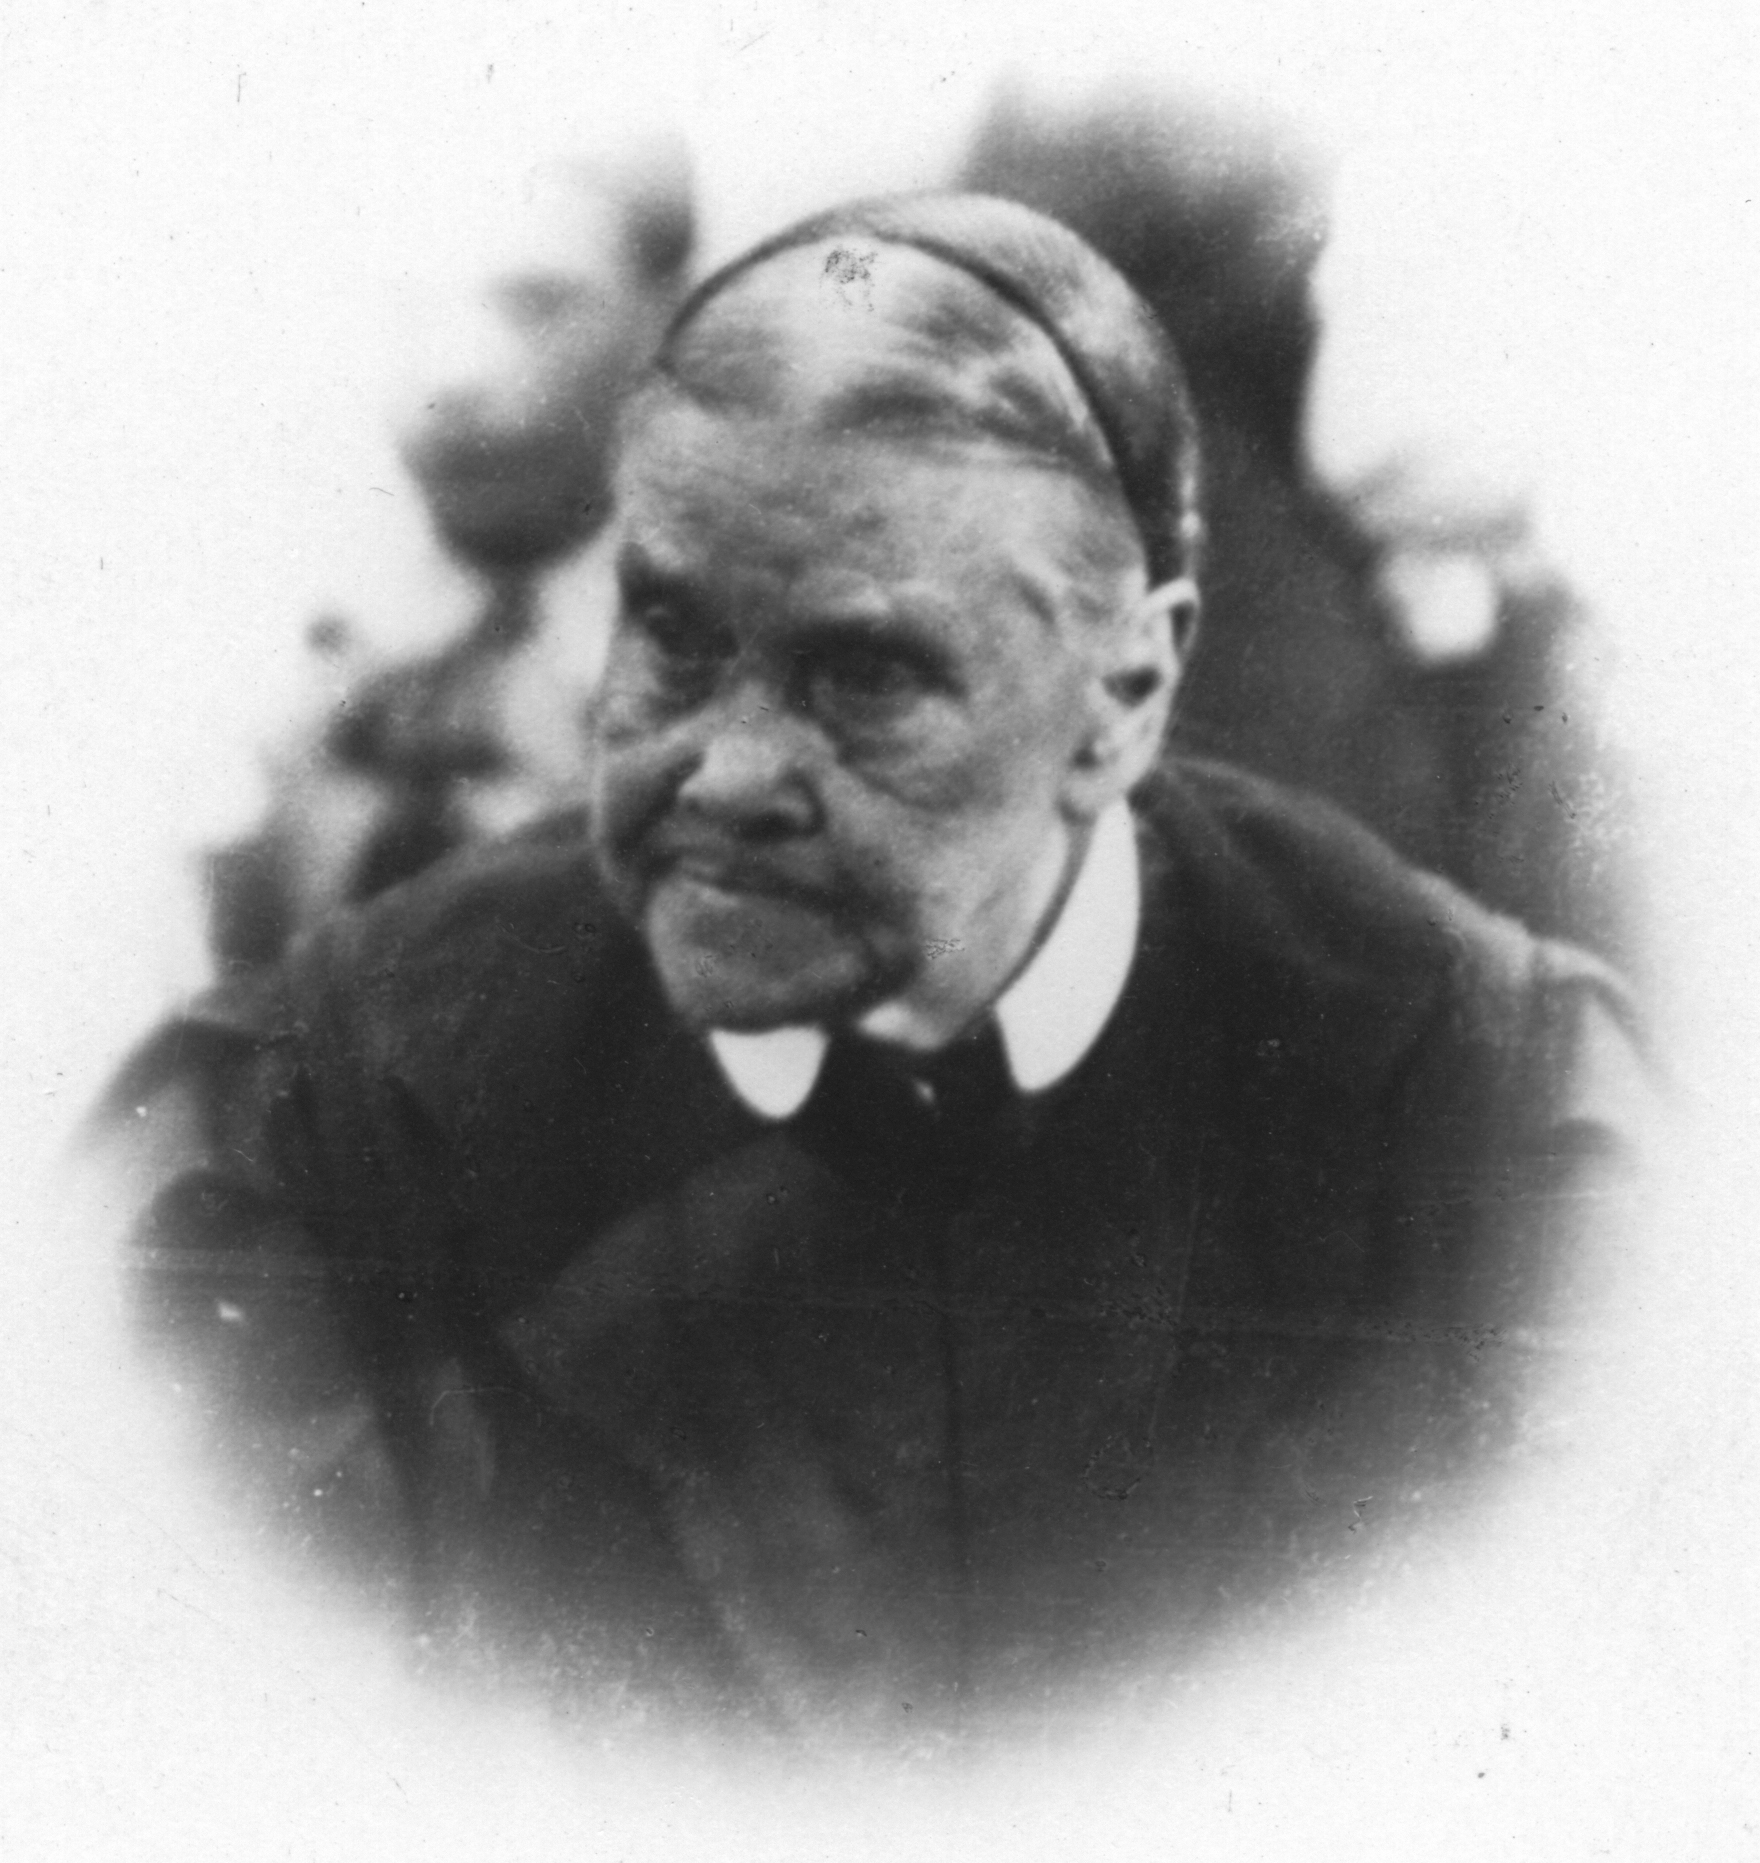
\includegraphics[width=1\linewidth]{images/ellen-white-1913.jpg}
    \caption*{Ellen G. White, 1913}
    \label{fig:e-white-1913}
\end{figure}

Siostra White przepowiedziała nam przyszłość. Dziś obserwujemy jej spełnienie. Porównując \emcap{Fundamentalne Zasady} z dzisiejszymi Fundamentalnymi Wierzeniami, widzimy, że nasza religia się zmieniła. Nasze przekonanie dotyczące \emcap{osobowości Boga} się zmieniło. Zostały napisane książki nowego porządku, które nie są oparte na solidnym Słowie Bożym. Został wprowadzony system filozofii intelektualnej.

Ta reformacja miała miejsce w jej czasach. Tak opisała dni Kościoła Adwentystów Dnia Siódmego w jej czasach i w przyszłości:

\egw{Obecny czas jest poważnym, pełnym trwogi czasem dla kościoła. Aniołowie są już przepasani, oczekując na rozkaz Boga, aby wylać swoje czasze gniewu na świat. Aniołowie zniszczenia podejmują dzieło zemsty, ponieważ Duch Boży stopniowo wycofuje się ze świata. Szatan również gromadzi swoje siły zła, wychodząc ‘do królów ziemi i całego świata’, aby zgromadzić ich pod swoim sztandarem, i przygotować do ‘bitwy w ów wielki dzień Boga Wszechmogącego.’ \textbf{Szatan podejmie najpotężniejsze wysiłki, aby zdobyć panowanie w ostatnim wielkim konflikcie. \underline{Fundamentalne zasady zostaną wydobyte na światło dzienne i zostaną podjęte decyzje w odniesieniu do nich}. Sceptycyzm przeważa wszędzie}. Bezbożność obfituje. \textbf{Wiara poszczególnych członków kościoła będzie poddana próbie, jakby nie było innej osoby na świecie}...}[Ms1a-1890.8; 1890][https://egwwritings.org/?ref=en\_Ms1a-1890.8&para=6780.13]

Najpotężniejsze wysiłki Szatana mają na celu usunięcie \emcap{Fundamentalnych Zasad} poprzez zasłonięcie ich sceptycyzmem. Oceniając z dzisiejszej perspektywy, poświadczamy prawdziwość proroctw Ellen White.

\egw{Mówię wam teraz, że kiedy zostanę złożona do grobu, \textbf{nastąpią wielkie zmiany}.}[Ms1-1915.2; 1915][https://egwwritings.org/?ref=en\_Ms1-1915.2&para=10771.9]

Prawdziwym pytaniem, które musimy sobie zadać  jest to: gdy \emcap{Fundamentalne Zasady} zostaną przedstawione, jaką decyzję podejmę w odniesieniu do nich? Czy nie powinniśmy odrzucić wszystkiego, co nie jest zgodne z tymi zasadami? Jaką decyzję podejmiesz?

\begin{titledpoem}

    \stanza{
        Proroctwa wczesny jeszcze głos \\
        Przewidział, jaki będzie los. \\
        „Diabeł ma spisek nam przeciwny, \\
        By wykraść prawdy w sposób dziwny”.
    }

    \stanza{
        Zasady, które niegdyś były, \\
        Które od Boga pochodziły, \\
        Na piasku teraz się ruszają, \\
        Bo ludzie Boga nie słuchają.
    }

    \stanza{
        Idee przebrane za światło, \\
        Usunąć filary tak łatwo. \\
        Książki też były przepisane, \\
        Nowe teorie nauczane.
    }

    \stanza{
        Czy szabat też mamy porzucić \\
        I tak od Boga się odwrócić? \\
        „Podstawy runą” — tak się zdaje, \\
        Gdy duma w miejsce prawdy staje.
    }

    \stanza{
        Wspomnijcie, jak żeśmy zaczęli, \\
        Gdy żeśmy prawdę w sercach mieli. \\
        Lecz poprzez podstępy szatana \\
        Teraz już prawda jest niechciana.
    }

    \stanza{
        Powróćmy zatem do przeszłości, \\
        Do wczesnej wiary i wierności, \\
        Bo miał zapewnić głos proroczy, \\
        Że z dobrej ścieżki nikt nie zboczy.
    }

    \stanza{
        Przetrwajmy burzę, która trwa, \\
        Gdyż warta tego prawda ta. \\
        Głosowi Ellen więc uwierzmy \\
        I prawdę drogą tak wybierzmy.
    }

    \stanza{
        A zanim przyjdzie na świat trwoga, \\
        Ustawmy się po stronie Boga. \\
        Ze starych ścieżek nie zbaczajmy \\
        I zepchnąć z nich się już nie dajmy.
    }

\end{titledpoem}
          % Chapter 24
\chapter{Setting up the wrong Fundamental Principles}


\chapter{Ustanawianie niewłaściwych Fundamentalnych Zasad}


You might ask yourself: how could it be possible that we, as a church, have gone astray from the light God gave us in the beginning? The answer to this question is the same answer to the question why the Jews went astray from the light God gave them concerning His Son. Please, take a look at the driving force behind the church in Apostolic times and our time.


Możesz zadać sobie pytanie: jak to możliwe, że my, jako kościół, odeszliśmy od światła, które Bóg dał nam na początku? Odpowiedź na to pytanie jest taka sama jak odpowiedź na pytanie, dlaczego Żydzi odeszli od światła, które Bóg dał im odnośnie Jego Syna. Proszę, spójrz na siłę napędową kościoła w czasach apostolskich i w naszych czasach.


\egw{‘The angel of the Lord by night opened the prison doors, and brought them forth, and said, Go, stand and speak in the temple to the people all the words of this life.’ [Acts 5:19, 20.] We see here that the men in authority are not always obeyed, even though they may profess to be teachers of Bible doctrines. \textbf{There are many today who feel indignant and aggrieved that any voice should be raised presenting ideas that differ from their own in regard to points of religious belief}. \textbf{Have they not long advocated their ideas as truth?} So the priests and rabbis reasoned in apostolic days. What mean these men who are unlearned, some of them mere fishermen, who are presenting ideas contrary to the doctrines which the learned priests and rulers are teaching the people? \textbf{They have no right to meddle with the fundamental principles of our faith}.}[Lt38-1896.23; 1896][https://egwwritings.org/?ref=en\_Lt38-1896.23&para=5631.29]


\egw{‘Anioł Pański w nocy otworzył drzwi więzienia i wyprowadził ich, i powiedział: Idźcie, stańcie i mówcie w świątyni do ludzi wszystkie słowa tego życia.’ [Dz 5:19, 20.] Widzimy tutaj, że ludzie sprawujący władzę nie zawsze są słuchani, nawet jeśli mogą twierdzić, że są nauczycielami doktryn biblijnych. \textbf{Jest dziś wielu, którzy czują się oburzeni i pokrzywdzeni, że jakikolwiek głos przedstawia idee różniące się od ich własnych w odniesieniu do punktów wiary religijnej}. \textbf{Czy nie głosili od dawna swoich idei jako prawdy?} Tak rozumowali kapłani i rabini w czasach apostolskich. Co znaczą ci niewykształceni ludzie, niektórzy z nich zwykli rybacy, którzy przedstawiają idee sprzeczne z doktrynami, których uczeni kapłani i przywódcy nauczają lud? \textbf{Nie mają prawa ingerować w fundamentalne zasady naszej wiary}.}[Lt38-1896.23; 1896][https://egwwritings.org/?ref=en\_Lt38-1896.23&para=5631.29]


\egwnogap{“\textbf{But we see that the God of heaven sometimes commissions men to \underline{teach that which is regarded as contrary to the established doctrines}. Because those who were once the depositaries of truth \underline{became unfaithful to their sacred trust}, the Lord chose others who would receive the bright beams of the Sun of Righteousness, and would advocate truths that were not in accordance with the ideas of the religious leaders. And then these leaders, in the blindness of their minds, give full sway to what is supposed to be righteous indignation against the ones who have set aside cherished fables. They act like men that have lost their reason. They do not consider the possibility that they themselves have not rightly understood the Word. They will not open their eyes to discern the fact that they have misinterpreted and misapplied the Scriptures, and have built up false theories, \underline{calling them fundamental doctrines of the faith}}.“}[Lt38-1896.24; 1896][https://egwwritings.org/?ref=en\_Lt38-1896.24&para=5631.30]


\egwnogap{“\textbf{Ale widzimy, że Bóg niebios czasami powołuje ludzi, aby \underline{nauczali tego, co jest uważane za sprzeczne z ustalonymi doktrynami}. Ponieważ ci, którzy kiedyś byli depozytariuszami prawdy, \underline{stali się niewierni swojemu świętemu zadaniu}, Pan wybrał innych, którzy przyjęliby jasne promienie Słońca Sprawiedliwości i głosiliby prawdy, które nie były zgodne z ideami przywódców religijnych. A wtedy ci przywódcy, w zaślepieniu swoich umysłów, dają pełną swobodę temu, co uważają za sprawiedliwe oburzenie przeciwko tym, którzy odrzucili ukochane bajki. Zachowują się jak ludzie, którzy stracili rozum. Nie biorą pod uwagę możliwości, że sami mogli niewłaściwie zrozumieć Słowo. Nie otworzą oczu, aby dostrzec fakt, że błędnie interpretowali i niewłaściwie stosowali Pisma, i zbudowali fałszywe teorie, \underline{nazywając je fundamentalnymi doktrynami wiary}}.”}[Lt38-1896.24; 1896][https://egwwritings.org/?ref=en\_Lt38-1896.24&para=5631.30]


\egwnogap{\textbf{But the Holy Spirit will from time to time reveal the truth through its own chosen agencies; and no man, not even a priest or ruler, has a right to say, You shall not give publicity to your opinions, because I do not believe them. That wonderful ‘I’ may attempt to put down the Holy Spirit’s teaching. Men may, for a time, attempt to smother it and kill it; but that will not make error truth or truth error. The inventive minds of men have advanced speculative opinions in various lines, and when the Holy Spirit lets light shine into human minds, it does not respect every point of man’s application of the word. God impressed his servants to speak the truth irrespective of what men had taken for granted as truth}.}[Lt38-1896.25; 1896][https://egwwritings.org/?ref=en\_Lt38-1896.25&para=5631.31]


\egwnogap{\textbf{Ale Duch Święty będzie od czasu do czasu objawiał prawdę przez swoje wybrane narzędzia; i żaden człowiek, nawet kapłan czy władca, nie ma prawa powiedzieć: Nie wolno ci upubliczniać swoich opinii, ponieważ ja w nie nie wierzę. To cudowne ‘Ja’ może próbować stłumić nauczanie Ducha Świętego. Ludzie mogą przez pewien czas próbować je zdusić i zabić; ale to nie sprawi, że błąd stanie się prawdą lub prawda błędem. Pomysłowe umysły ludzi wysunęły spekulatywne opinie w różnych kierunkach, a kiedy Duch Święty pozwala, aby światło zaświeciło w ludzkich umysłach, nie respektuje każdego punktu ludzkiego zastosowania słowa. Bóg natchnął swoich sług, aby mówili prawdę bez względu na to, co ludzie uznali za pewnik jako prawdę}.}[Lt38-1896.25; 1896][https://egwwritings.org/?ref=en\_Lt38-1896.25&para=5631.31]


\egwnogap{\textbf{\underline{Even Seventh-day Adventists are in danger of closing their eyes to truth as it is in Jesus}, because it contradicts something which they have taken for granted as truth, but which the Holy Spirit teaches is not truth. Let all be very modest, and seek most earnestly to put self out of the question, and to exalt Jesus.} \textbf{In most of the religious controversies, the foundation of the trouble is that self is striving for the supremacy}. About what? About matters which are not vital points at all, and which are regarded as such only because men have given importance to them. See Matthew 12:31-37; Mark 14:56; Luke 5:21; Matthew 9:3.}[Lt38-1896.26; 1896][https://egwwritings.org/?ref=en\_Lt38-1896.26&para=5631.32]


\egwnogap{\textbf{\underline{Nawet Adwentyści Dnia Siódmego są w niebezpieczeństwie zamknięcia oczu na prawdę, jaką jest w Jezusie}, ponieważ przeczy ona czemuś, co uznali za pewnik jako prawdę, ale czego Duch Święty uczy, że nie jest prawdą. Niech wszyscy będą bardzo skromni i niech gorliwie starają się usunąć siebie z tego zagadnienia, a wywyższać Jezusa.} \textbf{W większości kontrowersji religijnych podstawą problemu jest to, że własne ja walczy o supremację}. O co? O sprawy, które wcale nie są kluczowymi punktami, a są uważane za takie tylko dlatego, że ludzie nadali im znaczenie. Zobacz Mateusza 12:31-37; Marka 14:56; Łukasza 5:21; Mateusza 9:3.}[Lt38-1896.26; 1896][https://egwwritings.org/?ref=en\_Lt38-1896.26&para=5631.32]


The proud state of the heart resists the will of God and is the driving force behind apostasy; the humble heart is obedient to the will of God and is the driving force behind true reformation. The following quotations express future, concrete prophecies where the fanciful ideas of God will be brought in and \egwinline{many things of like character will in the future arise}[Ms137-1903.10; 1903][https://egwwritings.org/?ref=en\_Ms137-1903.10&para=9939.17]. These ideas are of like character to the ideas contained in the Living Temple. They will do away with the \emcap{personality of God}. Ellen White gives warning after warning to adhere to the \emcap{Fundamental Principles}, and to be aware of the leaders who will tear down the old foundation.


Dumny stan serca sprzeciwia się woli Bożej i jest siłą napędową odstępstwa; pokorne serce jest posłuszne woli Bożej i jest siłą napędową prawdziwej reformacji. Poniższe cytaty wyrażają przyszłe, konkretne proroctwa, gdzie fantazyjne idee o Bogu zostaną wprowadzone i \egwinline{wiele rzeczy o podobnym charakterze pojawi się w przyszłości}[Ms137-1903.10; 1903][https://egwwritings.org/?ref=en\_Ms137-1903.10&para=9939.17]. Te idee mają podobny charakter do idei zawartych w The Living Temple. Zniosą one \emcap{osobowość Boga}. Ellen White daje ostrzeżenie za ostrzeżeniem, aby trzymać się \emcap{Fundamentalnych Zasad} i być świadomym przywódców, którzy będą burzyć stary fundament.


\egw{In view of these Scriptures, who will dare to interpret God and place in the minds of others the sentiments regarding Him that are contained in Living Temple? \textbf{These theories are the theories of the great deceiver, and in the lives of \underline{those who receive them there will be sad chapters}}. \textbf{This is Satan’s device \underline{to unsettle the foundation of our faith}, to shake our confidence in the Lord’s guidance and in the experience that He has given us. \underline{Many things of like character will in the future arise}}. I entreat our medical missionary workers to be afraid to trust the suppositions and devising of any human being who entertains the thought that \textbf{the path over which the people of God have been led for the last fifty years is a wrong path}. \textbf{\underline{Beware of those who}, not having had any decided experience in the leading of the Lord’s Spirit, \underline{would suppose that this leading is all a fallacy}; that we have not the truth}; that we are not the people of the Lord, gathered by Him from all countries and nations. \textbf{\underline{Beware of those who would tear down the foundation, upon which we have been building for the last fifty years, to establish a new doctrine}}. \textbf{I know that these new theories are from the enemy}.}[Ms137-1903.10; 1903][https://egwwritings.org/?ref=en\_Ms137-1903.10&para=9939.17]


\egw{W świetle tych fragmentów Pisma, kto odważy się interpretować Boga i umieszczać w umysłach innych poglądy na Jego temat, które są zawarte w Living Temple? \textbf{Te teorie są teoriami wielkiego zwodziciela, a w życiu \underline{tych, którzy je przyjmują, będą smutne rozdziały}}. \textbf{To jest narzędzie Szatana, \underline{aby zachwiać fundamentem naszej wiary}, zachwiać naszym zaufaniem do prowadzenia Pana i do doświadczenia, które nam dał. \underline{Wiele rzeczy o podobnym charakterze pojawi się w przyszłości}}. Błagam naszych pracowników misji medycznej, aby bali się ufać przypuszczeniom i pomysłom jakiejkolwiek istoty ludzkiej, która żywi myśl, że \textbf{ścieżka, po której lud Boży był prowadzony przez ostatnie pięćdziesiąt lat, jest niewłaściwą ścieżką}. \textbf{\underline{Strzeżcie się tych, którzy}, nie mając żadnego zdecydowanego doświadczenia w prowadzeniu Ducha Pańskiego, \underline{przypuszczaliby, że to prowadzenie jest całkowitą pomyłką}; że nie mamy prawdy}; że nie jesteśmy ludem Pana, zgromadzonym przez Niego ze wszystkich krajów i narodów. \textbf{\underline{Strzeżcie się tych, którzy chcieliby zburzyć fundament, na którym budowaliśmy przez ostatnie pięćdziesiąt lat, aby ustanowić nową doktrynę}}. \textbf{Wiem, że te nowe teorie pochodzą od wroga}.}[Ms137-1903.10; 1903][https://egwwritings.org/?ref=en\_Ms137-1903.10&para=9939.17]


\egwnogap{\textbf{Let those who would \underline{bring in} fanciful ideas of God awake to a sense of their danger. This is too solemn a subject to be trifled with}.}[Ms137-1903.11; 1903][https://egwwritings.org/?ref=en\_Ms137-1903.11&para=9939.18]


\egwnogap{\textbf{Niech ci, którzy chcieliby \underline{wprowadzić} fantazyjne idee o Bogu, obudzą się i zrozumieją swoje niebezpieczeństwo. To zbyt poważny temat, aby się nim bawić}.}[Ms137-1903.11; 1903][https://egwwritings.org/?ref=en\_Ms137-1903.11&para=9939.18]


\egwnogap{The root of idolatry is an evil heart of unbelief in departing from the living God. It is because men have not faith in the presence and power of God \textbf{that they have been putting their trust in their own wisdom}. They have been devising and planning to exalt themselves and find salvation in their own works. \textbf{\underline{A deceptive influence from satanic agencies is coming in}, because leaders whom the Lord has warned and entreated and counseled are choosing their own wisdom in the place of the wisdom of God}. To such ones the warning comes, ‘Talk no more exceedingly proudly; let not arrogancy come out of your mouth; for the Lord is a God of knowledge, and by Him actions are weighed.’}[Ms137-1903.12; 1903][https://egwwritings.org/?ref=en\_Ms137-1903.12&para=9939.19]


\egwnogap{Korzeniem bałwochwalstwa jest złe serce niewiary, odchodzące od żywego Boga. To dlatego, że ludzie nie mają wiary w obecność i moc Boga, \textbf{pokładali zaufanie w swojej własnej mądrości}. Wymyślali i planowali, aby wywyższyć samych siebie i znaleźć zbawienie w swoich własnych uczynkach. \textbf{\underline{Zwodniczy wpływ z szatańskich agencji nadchodzi}, ponieważ przywódcy, których Pan ostrzegał, błagał i radził, wybierają swoją własną mądrość zamiast mądrości Bożej}. Do takich przychodzi ostrzeżenie: ‘Nie mówcie więcej tak bardzo dumnie; niech nie wychodzi z ust waszych arogancja; gdyż Pan jest Bogiem wiedzy i przez Niego uczynki są ważone.’}[Ms137-1903.12; 1903][https://egwwritings.org/?ref=en\_Ms137-1903.12&para=9939.19]


Comparing the old \emcap{Fundamental Principles} with the new trinitarian Fundamental Beliefs, we see the difference. We see that we’ve stepped off of the foundation of our faith and built a new one. This has been a process. Today, as it was in the days of Sister White, satanic agencies have brought a deceptive influence into the Seventh-day Adventist Church, \egwinline{because leaders whom the Lord has warned and entreated and counseled are choosing their own wisdom in the place of the wisdom of God}. We should \egwinline{\textbf{Beware of those who would tear down the foundation, upon which we have been building for the last fifty years, to establish a new doctrine}.}


Porównując stare \emcap{Fundamentalne Zasady} z nowymi trynitarnymi Fundamentalnymi Wierzeniami, widzimy różnicę. Widzimy, że zeszliśmy z fundamentu naszej wiary i zbudowaliśmy nowy. To był proces. Dziś, tak jak za czasów Siostry White, szatańskie siły wprowadziły zwodniczy wpływ do Kościoła Adwentystów Dnia Siódmego, \egwinline{ponieważ przywódcy, których Pan ostrzegał, błagał i którym doradzał, wybierają własną mądrość zamiast mądrości Boga}. Powinniśmy \egwinline{\textbf{Wystrzegać się tych, którzy chcieliby zburzyć fundament, na którym budowaliśmy przez ostatnie pięćdziesiąt lat, aby ustanowić nową doktrynę}.}


% Setting up the wrong Fundamental Principles

\begin{titledpoem}
    
    \stanza{
        In the silence of our own church’s walls, \\
        We’ve strayed from the light that first on us falls. \\
        An ancient query resounds with age: \\
        Why from sacred paths do we disengage?
    }

    \stanza{
        Ellen spoke of priests and rabbis of old, \\
        Men of cloth, with hearts yet so cold. \\
        They spurned the truth when it brightly shone, \\
        Proud hearts rejecting what was divinely shown.
    }

    \stanza{
        Behold the fishermen with unlearned tongues, \\
        Who dared to challenge the learned ones. \\
        "The Holy Spirit guides," they boldly claimed, \\
        While leaders scorned and fiercely blamed.
    }

    \stanza{
        Do not the humble hearts perceive \\
        The quiet whispers they should believe? \\
        While proud hearts preach their own command, \\
        True faith slips like fine sand from hand.
    }

    \stanza{
        Even now, echoes of the past, \\
        Warn us of shadows that leaders cast. \\
        God’s own voice, through years does span, \\
        Yet resisted by the inventions of man.
    }

    \stanza{
        To the foundations we must hold fast, \\
        Not swayed by shadows that leaders cast. \\
        For in the Scripture’s unerring light, \\
        Lies the path that is just and right.
    }

    \stanza{
        Beware of new doctrines, thinly veiled, \\
        On old, firm rocks they have not sailed. \\
        Let not man’s wisdom lead astray, \\
        But God’s own Spirit show the way.
    }

    \stanza{
        In faith, let us each day commence, \\
        With Bible as shield, no human pretense. \\
        For truth in Christ alone is found, \\
        And on this rock, our faith is sound.
    }
    
\end{titledpoem}

% \begin{titledpoem}

    \stanza{
        Niestety w naszych własnych ścianach \\
        Z kazalnic prawda jest ściągana. \\
        Ludzie wolą pochlebne baśnie, \\
        Aż cała czujność w każdym zaśnie.
    }

    \stanza{
        Starsi wraz z pastorami rządzą, \\
        Podczas gdy ludzie w grzechu błądzą. \\
        Laodycea wciąż się chwali, \\
        Lecz wkrótce zbiorą to, co siali.
    }

    \stanza{
        Do starych ścieżek powracajcie \\
        I ani sworznia nie ruszajcie. \\
        Prawdę stopniowo odrzucali \\
        I mocy Ducha nie poznali.
    }

    \stanza{
        Czy serce nie odczuwa tego, \\
        Że prawda zbliża się do niego? \\
        Tymczasem bajki uszy tuczą, \\
        Od Boga się niechętnie uczą.
    }

    \stanza{
        Strzeżcie się błędu zakrytego \\
        Z ręki człowieka ułomnego. \\
        Strzeżcie się swych przywódców cieni, \\
        Bo błędem będziecie zwiedzeni.
    }

    \stanza{
        Sprowadza z drogi mądrość człeka, \\
        Więc Bóg niech prowadzi człowieka. \\
        A w jasnym świetle prosto z Pisma \\
        Jest nasza ścieżka, nasza przystań.
    }

    \stanza{
        Niech każdy dzień się zacznie w wierze \\
        I Słowo będzie Twym puklerzem, \\
        Gdyż prawda jest w Chrystusie stała \\
        A wiara w Niego — nasza skała.
    }

\end{titledpoem}
          % Chapter 25
\chapter{The steps to Omega}


\chapter{Kroki do Omegi}


In our study so far, we have seen evidence that Kellogg’s controversy was connected to the Trinity doctrine and the \emcap{personality of God} expressed in the first point of the \emcap{Fundamental Principles}. Unfortunately, today we do not stand on that foundation regarding the \emcap{personality of God}; we have built another foundation that has changed the truth on the \emcap{personality of God} to a mysterious Triune God. Sister White was clearly against this reorganization and she prophesied that in the closing of His work, God will rehearse the history of the Advent movement and re-establish every pillar of our faith that was held in the beginning.


W naszym dotychczasowym studium widzieliśmy dowody, że kontrowersja Kellogga była związana z doktryną o Trójcy i \emcap{osobowością Boga} wyrażoną w pierwszym punkcie \emcap{Fundamentalnych Zasad}. Niestety, dzisiaj nie stoimy na tym fundamencie dotyczącym \emcap{osobowości Boga}; zbudowaliśmy inny fundament, który zmienił prawdę o \emcap{osobowości Boga} w tajemniczego Trójjedynego Boga. Siostra White była wyraźnie przeciwna tej reorganizacji i przepowiedziała, że przy końcu Swojego dzieła Bóg powtórzy historię ruchu adwentowego i przywróci każdy filar naszej wiary, który był utrzymywany na początku.


\egw{\textbf{\underline{The Lord has declared that the history of the past shall be rehearsed as we enter upon the closing work}. \underline{Every truth} that He has given for these last days is to be proclaimed to the world. \underline{Every pillar} that He has established \underline{is to be strengthened}. We cannot now step off the foundation that God has established. We cannot now enter into any new organization; for this would mean apostasy from the truth}.}[Ms129-1905.6; 1905][https://egwwritings.org/?ref=en\_Ms129-1905.6&para=9797.13]


\egw{\textbf{\underline{Pan oświadczył, że historia przeszłości zostanie powtórzona, gdy wkraczamy w końcowe dzieło}. \underline{Każda prawda}, którą dał na te ostatnie dni, ma być ogłoszona światu. \underline{Każdy filar}, który ustanowił, \underline{ma być wzmocniony}. Nie możemy teraz zejść z fundamentu, który Bóg ustanowił. Nie możemy teraz wejść w żadną nową organizację; oznaczałoby to odstępstwo od prawdy}.}[Ms129-1905.6; 1905][https://egwwritings.org/?ref=en\_Ms129-1905.6&para=9797.13]


Comparing the \emcap{Fundamental Principles} with the current Fundamental Beliefs of Seventh-day Adventists, we see that we have entered into a new organization. God’s warning, given through Sister White, to re-establish all pillars of our faith in these last days, is becoming imperative. As we traced the Trinity doctrine from Kellogg's controversy, we came across Ellen White’s warnings against alpha and omega apostasy, which will enter into our church.


Porównując \emcap{Fundamentalne Zasady} z obecnymi Fundamentalnymi Wierzeniami Adwentystów Dnia Siódmego, widzimy, że weszliśmy w nową organizację. Boże ostrzeżenie, przekazane przez Siostrę White, aby przywrócić wszystkie filary naszej wiary w tych ostatnich dniach, staje się naglące. Śledząc doktrynę o Trójcy od kontrowersji Kellogga, natrafiliśmy na ostrzeżenia Ellen White przed odstępstwem alfa i omega, które wejdzie do naszego kościoła.


\egw{\textbf{‘Living Temple’ contains the alpha of these theories. I knew that \underline{the omega would follow in a little while}; and I trembled for our people}. I knew that \textbf{I must warn our brethren and sisters not to enter into controversy \underline{over the presence and personality of God}. The statements made in ‘Living Temple’ \underline{in regard to this point are incorrect}. }The scripture used to substantiate the doctrine there set forth, is scripture misapplied.}[SpTB02 53.2; 1904][https://egwwritings.org/?ref=en\_SpTB02.53.2&para=417.271]


\egw{\textbf{‘Living Temple’ zawiera alfę tych teorii. Wiedziałam, że \underline{omega nastąpi wkrótce}; i drżałam o nasz lud}. Wiedziałam, że \textbf{muszę ostrzec naszych braci i siostry, aby nie wchodzili w spór \underline{dotyczący obecności i osobowości Boga}. Stwierdzenia zawarte w ‘Living Temple’ \underline{odnośnie tego punktu są niepoprawne}. }Pismo Święte użyte do poparcia doktryny tam przedstawionej jest błędnie zastosowanym Pismem.}[SpTB02 53.2; 1904][https://egwwritings.org/?ref=en\_SpTB02.53.2&para=417.271]


In the context of Seventh-day Adventist reorganization, we identify several steps that were necessary to accomplish this reorganization and are necessary to uphold it.


W kontekście reorganizacji Adwentystów Dnia Siódmego, identyfikujemy kilka kroków, które były niezbędne do dokonania tej reorganizacji i są konieczne do jej podtrzymania.


\subsection*{Step 1: Deny the Fundamental Principles to be the foundation of our faith and the official, and accurate, representation of Seventh-day Adventist beliefs}


\subsection*{Krok 1: Zaprzeczenie, że Fundamentalne Zasady są fundamentem naszej wiary oraz oficjalną i dokładną reprezentacją wierzeń Adwentystów Dnia Siódmego}


The first step necessary is to hide the original foundation of our faith by unlinking it with the \emcap{Fundamental Principles}.


Pierwszym niezbędnym krokiem jest ukrycie oryginalnego fundamentu naszej wiary poprzez odłączenie go od \emcap{Fundamentalnych Zasad}.


\egw{\textbf{As a people, we are to \underline{stand firm on the platform of eternal truth} that has withstood test and trial. We are to \underline{hold to the sure pillars of our faith}. \underline{The principles of truth} that God has revealed to us \underline{are our only true foundation}. They have made us what we are. The lapse of time has not lessened their value. \underline{It is the constant effort of the enemy to remove these truths from their setting}, and to put in their place \underline{spurious theories}. He \underline{will bring in} everything that he possibly can to carry out his deceptive designs.}}[SpTB02 51.2; 1904][https://egwwritings.org/?ref=en\_SpTB02.51.2&para=417.261]


\egw{\textbf{Jako lud, mamy \underline{stać mocno na platformie wiecznej prawdy}, która wytrzymała próby i testy. Mamy \underline{trzymać się pewnych filarów naszej wiary}. \underline{Zasady prawdy}, które Bóg nam objawił, \underline{są naszym jedynym prawdziwym fundamentem}. One uczyniły nas tym, kim jesteśmy. Upływ czasu nie zmniejszył ich wartości. \underline{Nieustannym wysiłkiem wroga jest usunięcie tych prawd z ich kontekstu} i umieszczenie na ich miejscu \underline{fałszywych teorii}. On \underline{wprowadzi} wszystko, co tylko może, aby zrealizować swoje zwodnicze plany.}}[SpTB02 51.2; 1904][https://egwwritings.org/?ref=en\_SpTB02.51.2&para=417.261]


\egw{\textbf{Messages of every order and kind have been urged upon Seventh-day Adventists, to take the place of the truth which, \underline{point by point}, has been sought out by prayerful study, and testified to by the miracle-working power of the Lord}. \textbf{But \underline{the way-marks} \underline{which have made us what we are}, \underline{are to be preserved}, and they \underline{will be preserved}, as God has signified through His word and the testimony of His Spirit}. \textbf{He calls upon us to \underline{hold firmly}, with the grip of faith, to \underline{the fundamental principles} that are \underline{based upon unquestionable authority}}.}[SpTB02 59.1; 1904][https://egwwritings.org/?ref=en\_SpTB02.59.1&para=417.299]


\egw{\textbf{Przesłania wszelkiego rodzaju i typu były narzucane Adwentystom Dnia Siódmego, aby zająć miejsce prawdy, która, \underline{punkt po punkcie}, została odkryta przez modlitewne studium i potwierdzona przez cudowną moc Pana}. \textbf{Ale \underline{znaki}, które \underline{uczyniły nas tym, kim jesteśmy}, \underline{mają być zachowane} i \underline{będą zachowane}, jak Bóg oznajmił przez Swoje słowo i świadectwo Swojego Ducha}. \textbf{Wzywa nas, abyśmy \underline{trzymali się mocno}, z uściskiem wiary, \underline{fundamentalnych zasad}, które \underline{opierają się na niepodważalnym autorytecie}}.}[SpTB02 59.1; 1904][https://egwwritings.org/?ref=en\_SpTB02.59.1&para=417.299]


The \emcap{Fundamental Principles} were the truths God revealed to the pioneers after the passing of time in 1844. We have seen the testimonies of our pioneers, including Ellen White, regarding the first point of the \emcap{Fundamental Principles}. All of them were in harmony regarding these particular points of our faith. In 1863, Seventh-day Adventists organized themselves into a church, as an organized body. Since then, many were misrepresenting the position of the Seventh-day Adventist Church and the pioneers found it necessary to meet inquiries, \others{and sometimes to correct false statements circulated against} the church’s beliefs and practices. Consequently, in 1872, the pioneers issued the document called “\textit{A Declaration of the Fundamental Principles, Taught and Practiced by the Seventh-Day Adventists}”\footnote{“A Declaration of the Fundamental Principles, Taught and Practiced by the Seventh-Day Adventists (1872) : MVT : Free Download, Borrow, and Streaming : Internet Archive.” Internet Archive, 2025, \href{https://archive.org/details/ADeclarationOfTheFundamentalPrinciplesTaughtAndPracticedByThe}{archive.org/details/ADeclarationOfTheFundamentalPrinciplesTaughtAndPracticedByThe}. Accessed 3 Feb. 2025.}. This declaration presented the public with \others{a brief statement of what is, and has been, with great unanimity, held by}[The preface of the Fundamental Principles in 1872.] Seventh-day Adventists.


\emcap{Fundamentalne zasady} były prawdami, które Bóg objawił pionierom po upływie czasu w 1844 roku. Widzieliśmy świadectwa naszych pionierów, w tym Ellen White, dotyczące pierwszego punktu \emcap{Fundamentalnych zasad}. Wszyscy oni byli zgodni co do tych konkretnych punktów naszej wiary. W 1863 roku Adwentyści Dnia Siódmego zorganizowali się w kościół, jako zorganizowane ciało. Od tego czasu wielu błędnie przedstawiało stanowisko Kościoła Adwentystów Dnia Siódmego, a pionierzy uznali za konieczne odpowiadanie na zapytania, \others{a czasami korygowanie fałszywych stwierdzeń rozpowszechnianych przeciwko} wierzeniom i praktykom kościoła. W konsekwencji, w 1872 roku, pionierzy wydali dokument zatytułowany “\textit{Oświadczenie o fundamentalnych zasadach nauczanych i wyznawanych przez Adwentystów Dnia Siódmego}”\footnote{“A Declaration of the Fundamental Principles, Taught and Practiced by the Seventh-Day Adventists (1872) : MVT : Free Download, Borrow, and Streaming : Internet Archive.” Internet Archive, 2025, \href{https://archive.org/details/ADeclarationOfTheFundamentalPrinciplesTaughtAndPracticedByThe}{archive.org/details/ADeclarationOfTheFundamentalPrinciplesTaughtAndPracticedByThe}. Accessed 3 Feb. 2025.}. Ta deklaracja przedstawiła opinii publicznej \others{krótkie oświadczenie o tym, co jest i było, z wielką jednomyślnością, wyznawane przez}[Przedmowa do Fundamentalnych zasad z 1872 roku.] Adwentystów Dnia Siódmego.


In the chapter “\hyperref[chap:authority]{The Authority of the Fundamental Principles}”, we discussed how pro-Trinitarian scholars have been compromising the authority of the \emcap{Fundamental Principles}, denying their true value in our Adventist history.


W rozdziale “\hyperref[chap:authority]{Autorytet Fundamentalnych zasad}”, omówiliśmy, jak uczeni popierający Trójcę kompromitują autorytet \emcap{Fundamentalnych zasad}, zaprzeczając ich prawdziwej wartości w naszej adwentystycznej historii.


Pro-trinitarian scholars argue that this declaration was not what it claims to be—a declaration of the \emcap{fundamental principles}, taught and practiced by the Seventh-day Adventists. This declaration was a summary of the principal features of Adventist’s faith, and no point is really as problematic or objectionable as the first point, dealing with the \emcap{personality of God} and where His presence is. But the evidence in favor of the \emcap{Fundamental Principles}, especially to the first point, is overwhelming.


Uczeni popierający Trójcę twierdzą, że ta deklaracja nie była tym, co twierdzi - deklaracją \emcap{fundamentalnych zasad}, nauczanych i praktykowanych przez Adwentystów Dnia Siódmego. Ta deklaracja była podsumowaniem głównych cech wiary adwentystycznej, a żaden punkt nie jest naprawdę tak problematyczny lub kontrowersyjny jak pierwszy punkt, dotyczący \emcap{osobowości Boga} i tego, gdzie jest Jego obecność. Ale dowody na korzyść \emcap{Fundamentalnych zasad}, szczególnie pierwszego punktu, są przytłaczające.


All of these claims are easily refuted by the fact that the \emcap{Fundamental Principles} have been regularly issued and reprinted over the course of the entire life of Sister White, until 1914. If they were mere private opinions of a few individuals, as claimed by scholars\footnote{Ministry Magazine “Our Declaration of Fundamental Beliefs”: January 1958, Roy Anderson, J. Arthur Buckwalter, Louise Kleuser, Earl Cleveland and Walter Schubert}, would they have been consistently reprinted over the course of 42 years\footnote{For a detailed list of publications throughout these years, see the Appendix.}, publicly claiming to represent the synopsis of Seventh-day Adventist faith? If they had been issued only once, we could deem it a conspiracy by some individuals to purposely misrepresent Seventh-day Adventist faith. On the contrary, the \emcap{Fundamental Principles} were regularly reprinted, and they truly represented the official Seventh-day Adventist faith and practice.


Wszystkie te twierdzenia są łatwo obalone przez fakt, że \emcap{Fundamentalne zasady} były regularnie wydawane i przedrukowywane przez całe życie Siostry White, aż do 1914 roku. Gdyby były jedynie prywatnymi opiniami kilku osób, jak twierdzą uczeni\footnote{Ministry Magazine “Our Declaration of Fundamental Beliefs”: January 1958, Roy Anderson, J. Arthur Buckwalter, Louise Kleuser, Earl Cleveland and Walter Schubert}, czy byłyby konsekwentnie przedrukowywane przez 42 lata\footnote{Szczegółową listę publikacji w tych latach można znaleźć w Załączniku.}, publicznie twierdząc, że reprezentują streszczenie wiary Adwentystów Dnia Siódmego? Gdyby zostały wydane tylko raz, moglibyśmy uznać to za spisek kilku osób, które celowo błędnie przedstawiały wiarę Adwentystów Dnia Siódmego. Przeciwnie, \emcap{Fundamentalne zasady} były regularnie przedrukowywane i naprawdę reprezentowały oficjalną wiarę i praktykę Adwentystów Dnia Siódmego.


Another argument is that Sister White approved the \emcap{Fundamental Principles} in her writings by explicitly referring to them, and also by teaching the same truths taught in the \emcap{Fundamental Principles}. The works of our pioneers are also in harmony with the statements in this Declaration of the \emcap{Fundamental Principles}. Considering all of these facts, it is inevitable that this declaration was truthful in its claims. This document was indeed a declaration of the \emcap{fundamental principles}, taught and practiced by the Seventh-day Adventist Church, representing a public \others{synopsis of our faith}, \others{a brief statement of what is, and has been, with great unanimity, held by} Seventh-day Adventists.\footnote{The preface of the Fundamental Principles in 1872.} As such, it accurately represents the Seventh-day Adventist belief and practice, and represents the foundation of Seventh-day Adventist faith in the time of Ellen White.


Innym argumentem jest to, że Siostra White zatwierdziła \emcap{Fundamentalne zasady} w swoich pismach, wyraźnie się do nich odnosząc, a także nauczając tych samych prawd, które są nauczane w \emcap{Fundamentalnych zasadach}. Prace naszych pionierów są również zgodne z oświadczeniami w tej Deklaracji \emcap{Fundamentalnych zasad}. Biorąc pod uwagę wszystkie te fakty, jest nieuniknione, że ta deklaracja była prawdziwa w swoich twierdzeniach. Ten dokument był rzeczywiście deklaracją \emcap{fundamentalnych zasad}, nauczanych i praktykowanych przez Kościół Adwentystów Dnia Siódmego, reprezentującą publiczne \others{streszczenie naszej wiary}, \others{krótkie oświadczenie o tym, co jest i było, z wielką jednomyślnością, wyznawane przez} Adwentystów Dnia Siódmego.\footnote{Przedmowa do Fundamentalnych zasad z 1872 roku.} Jako taki, dokładnie reprezentuje wierzenia i praktyki Adwentystów Dnia Siódmego i stanowi fundament wiary Adwentystów Dnia Siódmego w czasach Ellen White.


Today, in defense of the Trinity doctrine, Adventist historians boldly claim that when our pioneers were studying Adventist truths such as the sanctuary, investigative judgment, the Sabbath and other doctrines, they \others{did not study the subject of the doctrine of God}. These Adventist historians falsely claim that the doctrine of God \others{was not the question that they dealt at that time}[Denis Kaiser. “From Antitrinitarianism to Trinitarianism: The Adventist story” and Panelist. The God We Worship: A Godhead Symposium. Central California Conference, Dinuba, CA. March 23-24, 2018.]. Following this false claim, they present historical data on how Adventist doctrine gradually moved toward Trinitarian understanding. The truth is, there are some instances early on\footnote{The earliest mention of the Trinity doctrine, in a positive sense, was when M.C. Wilcox reprinted a non-Adventist article by Samuel Spear in Signs of the Times, December 7th, 1891 and December 14th, 1891} when the Trinity doctrine is mentioned in a positive light in our literature. But when you consider the fact that the Adventist church did have a positive position on the subject of the doctrine of God, as it was expressed in the \emcap{Fundamental Principles}, these instances cannot be interpreted as progressiveness in understanding, but rather an intrusion of the Trinity doctrine into the Seventh-day Adventist Church.


Dziś, w obronie doktryny o Trójcy, historycy adwentystyczni śmiało twierdzą, że kiedy nasi pionierzy studiowali adwentystyczne prawdy, takie jak świątynia, sąd śledczy, Sabat i inne doktryny, \others{nie studiowali tematu doktryny o Bogu}. Ci historycy adwentystyczni fałszywie twierdzą, że doktryna o Bogu \others{nie była kwestią, którą zajmowali się w tamtym czasie}[Denis Kaiser. “From Antitrinitarianism to Trinitarianism: The Adventist story” and Panelist. The God We Worship: A Godhead Symposium. Central California Conference, Dinuba, CA. March 23-24, 2018.]. Po tym fałszywym twierdzeniu przedstawiają dane historyczne o tym, jak doktryna adwentystyczna stopniowo zmierzała w kierunku trynitarnego zrozumienia. Prawda jest taka, że istnieją pewne wczesne przypadki\footnote{Najwcześniejsza wzmianka o doktrynie o Trójcy, w pozytywnym sensie, miała miejsce, gdy M.C. Wilcox przedrukował nieadwentystyczny artykuł Samuela Speara w Signs of the Times, 7 grudnia 1891 i 14 grudnia 1891}, kiedy doktryna o Trójcy jest wspominana w pozytywnym świetle w naszej literaturze. Ale gdy weźmie się pod uwagę fakt, że Kościół Adwentystów miał pozytywne stanowisko w kwestii doktryny o Bogu, wyrażone w \emcap{Fundamentalnych zasadach}, tych przypadków nie można interpretować jako postępu w zrozumieniu, ale raczej jako wtargnięcie doktryny o Trójcy do Kościoła Adwentystów Dnia Siódmego.


It is easy to refute the claim that Adventist pioneers did not understand the doctrine of God. If they did not understand it, they would have failed to proclaim the first angel’s message. We discussed this point in detail in the chapter “\hyperref[chap:remembering-the-beginning]{Remembering the beginning}”. The Seventh-day Adventist movement was not a failure, but a God-led, prophetic movement.


Łatwo jest obalić twierdzenie, że pionierzy adwentystyczni nie rozumieli doktryny o Bogu. Gdyby jej nie rozumieli, nie udałoby im się głosić poselstwa pierwszego anioła. Omówiliśmy ten punkt szczegółowo w rozdziale “\hyperref[chap:remembering-the-beginning]{Pamiętając początek}”. Ruch Adwentystów Dnia Siódmego nie był porażką, ale prowadzonym przez Boga, prorockim ruchem.


\subsection*{Step 2: Ignore the warnings of building a new foundation}


\subsection*{Krok 2: Ignorowanie ostrzeżeń przed budowaniem nowego fundamentu}


When the \emcap{Fundamental Principles} are removed from the equation, many of Ellen White’s warnings fail to shine in their true light and their true meaning does not resonate with the reader.


Kiedy \emcap{Fundamentalne zasady} są usunięte z równania, wiele ostrzeżeń Ellen White nie świeci w swoim prawdziwym świetle, a ich prawdziwe znaczenie nie rezonuje z czytelnikiem.


We have cited many quotations where Sister White warned the church not to step off the \emcap{Fundamental Principles}. We dealt with them in the chapter “\hyperref[chap:apostasy]{The great apostasy is soon to be realized}”, but we will mention one of the most prominent quotations again.


Cytowaliśmy wiele wypowiedzi, w których Siostra White ostrzegała kościół, aby nie odstępował od \emcap{Fundamentalnych zasad}. Zajmowaliśmy się nimi w rozdziale “\hyperref[chap:apostasy]{Wielkie odstępstwo wkrótce się zrealizuje}”, ale wspomnimy ponownie jeden z najbardziej znaczących cytatów.


\egw{\textbf{The enemy of souls has sought to bring in the supposition that a great reformation was to take place among Seventh-day Adventists, and that this reformation would \underline{consist in giving up the doctrines which stand as the pillars of our faith} and engaging in a process of reorganization}. Were this reformation to take place, what would result? \textbf{The principles of truth that God in His wisdom has given to the remnant church would be discarded. Our religion would be changed. \underline{The fundamental principles that have sustained the work for the last fifty years would be accounted as error}}. \textbf{A new organization would be established. Books of a new order would be written. A system of intellectual philosophy would be introduced}...}[Lt242-1903.13; 1903][https://egwwritings.org/?ref=en\_Lt242-1903.13&para=7767.20]


\egw{\textbf{Wróg dusz starał się wprowadzić przypuszczenie, że wśród Adwentystów Dnia Siódmego miała nastąpić wielka reforma, i że ta reforma \underline{polegałaby na porzuceniu doktryn, które stoją jako filary naszej wiary} i zaangażowaniu się w proces reorganizacji}. Gdyby ta reforma miała miejsce, co by z tego wynikło? \textbf{Zasady prawdy, które Bóg w swojej mądrości dał Kościołowi ostatków, zostałyby odrzucone. Nasza religia zostałaby zmieniona. \underline{Fundamentalne zasady, które podtrzymywały dzieło przez ostatnie pięćdziesiąt lat, zostałyby uznane za błąd}}. \textbf{Zostałaby ustanowiona nowa organizacja. Zostałyby napisane książki nowego porządku. Zostałby wprowadzony system filozofii intelektualnej}...}[Lt242-1903.13; 1903][https://egwwritings.org/?ref=en\_Lt242-1903.13&para=7767.20]


\egwnogap{Who has authority to begin such a movement? \textbf{We have our Bibles. We have our experience, attested to by the miraculous working of the Holy Spirit}. \textbf{We have a truth that admits of no compromise.} \textbf{\underline{Shall we not repudiate everything that is not in harmony with this truth}?}}[Lt242-1903.14; 1903][https://egwwritings.org/?ref=en\_Lt242-1903.14&para=7767.21]


\egwnogap{Kto ma upoważnienie do rozpoczęcia takiego ruchu? \textbf{Mamy nasze Biblie. Mamy nasze doświadczenie, potwierdzone cudownym działaniem Ducha Świętego}. \textbf{Mamy prawdę, która nie dopuszcza żadnego kompromisu.} \textbf{\underline{Czy nie powinniśmy odrzucić wszystkiego, co nie jest w harmonii z tą prawdą}?}}[Lt242-1903.14; 1903][https://egwwritings.org/?ref=en\_Lt242-1903.14&para=7767.21]


\subsection*{Step 3: Deny that the personality of God was the pillar of our faith and a part of the foundation of our faith}


\subsection*{Krok 3: Zaprzeczenie, że osobowość Boga była filarem naszej wiary i częścią fundamentu naszej wiary}


There is one Ellen White statement that apparently supports the claim that the \emcap{personality of God} was not a pillar of our faith. Another expression for “\textit{pillars of our faith}” is “\textit{landmarks}”. In the following quotations, Sister White lists several landmarks: the cleansing of the sanctuary, the three angels’ messages, the temple of God, the Sabbath and the non-immortality of the wicked.


Istnieje jedno stwierdzenie Ellen White, które pozornie popiera twierdzenie, że \emcap{osobowość Boga} nie była filarem naszej wiary. Innym wyrażeniem na “\textit{filary naszej wiary}” jest “\textit{znaki}”. W poniższych cytatach Siostra White wymienia kilka znaków: oczyszczenie świątyni, poselstwa trzech aniołów, świątynię Boga, Sabat i nieśmiertelność bezbożnych.


\egw{The passing of the time in 1844 was a period of great events, opening to our astonished eyes \textbf{the cleansing of the sanctuary transpiring in heaven}, and having decided relation to God’s people upon the earth, [also] \textbf{the first and second angels’ messages and the third}, unfurling the banner on which was inscribed, ‘The commandments of God and the faith of Jesus.’ [Revelation 14:12.] One of the landmarks under this message was \textbf{the temple of God}, seen by His truth-loving people in heaven, and the ark containing the law of God. The light of \textbf{the Sabbath} of the fourth commandment flashed its strong rays in the pathway of the transgressors of God’s law. The \textbf{non-immortality of the wicked} is an old landmark. \textbf{I can call to mind nothing more that can come under the head of the old landmarks}. All this cry about changing the old landmarks is all imaginary.}[Ms13-1889.9; 1889][https://egwwritings.org/?ref=en\_Ms13-1889.9&para=4179.14]


\egw{Upływ czasu w 1844 roku był okresem wielkich wydarzeń, otwierających naszym zdumionym oczom \textbf{oczyszczenie świątyni odbywające się w niebie} i mające zdecydowany związek z ludem Bożym na ziemi, [także] \textbf{poselstwa pierwszego i drugiego anioła oraz trzeciego}, rozwijające sztandar, na którym było napisane: ‘Przykazania Boże i wiara Jezusa.’ [Objawienie 14:12.] Jednym ze znaków pod tym poselstwem była \textbf{świątynia Boża}, widziana przez Jego miłujący prawdę lud w niebie, i arka zawierająca prawo Boże. Światło \textbf{Sabatu} z czwartego przykazania rzucało swoje silne promienie na ścieżkę przestępców prawa Bożego. \textbf{Nieśmiertelność bezbożnych} jest starym znakiem. \textbf{Nie mogę przypomnieć sobie niczego więcej, co mogłoby wchodzić pod nagłówek starych znaków}. Całe to wołanie o zmianę starych znaków jest całkowicie wyimaginowane.}[Ms13-1889.9; 1889][https://egwwritings.org/?ref=en\_Ms13-1889.9&para=4179.14]


At the end of this list of landmarks, or pillars of our faith, she states that she can recall nothing else that would fall under the category of the old landmarks. For many, this quotation serves as proof that the \emcap{personality of God} was neither an old landmark nor a pillar. It is true that in this quotation, Sister White did not explicitly mention the \emcap{personality of God}, but it would be implicitly included under the first angel’s message, as well as being an underlying doctrine of the Sanctuary message. Furthermore, there are other quotations from Sister White that explicitly include the \emcap{personality of God} as an old landmark or pillar of our faith.


Na końcu tej listy znaków, czyli filarów naszej wiary, stwierdza, że nie może przypomnieć sobie niczego innego, co wchodziłoby do kategorii starych znaków. Dla wielu ten cytat służy jako dowód, że \emcap{osobowość Boga} nie była ani starym znakiem, ani filarem. To prawda, że w tym cytacie Siostra White nie wspomniała wyraźnie o \emcap{osobowości Boga}, ale byłaby ona domyślnie zawarta w poselstwie pierwszego anioła, a także jako podstawowa doktryna poselstwa o Świątyni. Ponadto istnieją inne cytaty od Siostry White, które wyraźnie włączają \emcap{osobowość Boga} jako stary znak lub filar naszej wiary.


\egw{Those who seek to remove the \textbf{old landmarks} are not holding fast; they \textbf{are not remembering how they have received and heard}. Those who try to \textbf{\underline{bring in} theories that would remove \underline{the pillars of our faith}} \textbf{concerning the sanctuary}, \textbf{\underline{or concerning the personality of God or of Christ}, are working as blind men}. They are seeking to bring in uncertainties and to set the people of God \textbf{adrift}, without an anchor.}[Ms62-1905.14; 1905][https://egwwritings.org/?ref=en\_Ms62-1905.14&para=10026.20]


\egw{Ci, którzy starają się usunąć \textbf{stare znaki}, nie trzymają się mocno; \textbf{nie pamiętają, jak otrzymali i słyszeli}. Ci, którzy próbują \textbf{\underline{wprowadzić} teorie, które usunęłyby \underline{filary naszej wiary}} \textbf{dotyczące świątyni}, \textbf{\underline{lub dotyczące osobowości Boga lub Chrystusa}, działają jak ślepi ludzie}. Starają się wprowadzić niepewności i postawić lud Boży \textbf{na dryfie}, bez kotwicy.}[Ms62-1905.14; 1905][https://egwwritings.org/?ref=en\_Ms62-1905.14&para=10026.20]


Sister White also teaches us that the pillars of our faith constitute the foundation of our faith.


Siostra White uczy nas również, że filary naszej wiary stanowią fundament naszej wiary.


\egw{\textbf{What influence is it that would lead men at this stage of our history to work in an underhanded, powerful way \underline{to tear down the foundation of our faith},—the foundation that was laid at the beginning of our work by prayerful study of the word and by revelation? Upon \underline{this foundation} we have been building for \underline{the past fifty years}. Do you wonder that when I see the beginning of a work that would \underline{remove some of the pillars of our faith}, I have something to say? I must obey the command, ‘Meet it!’}}[SpTB02 58.1; 1904][https://egwwritings.org/?ref=en\_SpTB02.58.1&para=417.295]


\egw{\textbf{Jaki wpływ prowadzi ludzi na tym etapie naszej historii do działania w podstępny, potężny sposób, \underline{aby zburzyć fundament naszej wiary},—fundament, który został położony na początku naszej pracy przez modlitewne studiowanie słowa i przez objawienie? Na \underline{tym fundamencie} budujemy przez \underline{ostatnie pięćdziesiąt lat}. Czy dziwisz się, że kiedy widzę początek pracy, która \underline{usunęłaby niektóre z filarów naszej wiary}, mam coś do powiedzenia? Muszę być posłuszna rozkazowi: ‘Przeciwstaw się temu!’}}[SpTB02 58.1; 1904][https://egwwritings.org/?ref=en\_SpTB02.58.1&para=417.295]


Removing some of the pillars of our faith means tearing down the foundation of our faith. Elsewhere, Sister White said that tearing down or undermining the foundation of our faith is done by indoctrination of the sentiments regarding the \emcap{personality of God}.


Usunięcie niektórych filarów naszej wiary oznacza zburzenie fundamentu naszej wiary. W innym miejscu Siostra White powiedziała, że burzenie lub podważanie fundamentu naszej wiary odbywa się poprzez indoktrynację poglądów dotyczących \emcap{osobowości Boga}.


\egw{The college was taken out of Battle Creek; yet students are still called there, and there they \textbf{become indoctrinated with the very sentiments regarding the personality of God and Christ that would undermine the foundation of our faith}.}[Lt72-1906.5; 1906][https://egwwritings.org/?ref=en\_Lt72-1906.5&para=10013.11]


\egw{Kolegium zostało przeniesione z Battle Creek; jednak studenci nadal są tam wzywani i tam \textbf{zostają indoktrynowani poglądami dotyczącymi osobowości Boga i Chrystusa, które podważyłyby fundament naszej wiary}.}[Lt72-1906.5; 1906][https://egwwritings.org/?ref=en\_Lt72-1906.5&para=10013.11]


In light of these quotations we see positive testimony that the \emcap{personality of God} was part of the foundation of our faith. Furthermore, in chapter 10 of the special testimonies, entitled “\textit{The foundation of our faith}”, Sister White mentioned “\textit{Fundamental Principles}” using the synonyms “\textit{pillars of our faith}”, “\textit{waymarks}”, and “\textit{landmarks}”, when addressing the foundation of our faith.


W świetle tych cytatów widzimy pozytywne świadectwo, że \emcap{osobowość Boga} była częścią fundamentu naszej wiary. Ponadto, w rozdziale 10 specjalnych świadectw, zatytułowanym “\textit{Fundament naszej wiary}”, Siostra White wspomniała o “\textit{Fundamentalnych Zasadach}” używając synonimów “\textit{filary naszej wiary}”, “\textit{znaki}” i “\textit{punkty orientacyjne}”, odnosząc się do fundamentu naszej wiary.


\subsection*{Step 4: Alter the meaning of the term “the personality of God”}


\subsection*{Krok 4: Zmiana znaczenia terminu “osobowość Boga”}


The term ‘\textit{personality}’ has two different applications and the most common definition in everyday use is in the area of psychology. ‘\textit{Personality}’ is defined as “\textit{the characteristic sets of behaviors, cognitions, and emotional patterns that evolve from biological and environmental factors}”\footnote{Wikipedia Contributors. “Personality.” Wikipedia, Wikimedia Foundation, 19 Apr. 2019, \href{https://en.wikipedia.org/wiki/Personality}{en.wikipedia.org/wiki/Personality}.}. It is of utmost importance to recognize that when we are dealing with the pillar of our faith—“\textit{the personality of God}”—we are not in the realms of psychology. The accurate application of the word ‘\textit{personality}’ within the doctrine on the \emcap{personality of God} is found in the Merriam-Webster Dictionary: “\textit{the quality or state of being a person}”\footnote{\href{https://www.merriam-webster.com/dictionary/personality}{Merriam-Webster Dictionary} - ‘\textit{personality}’}. According to the Merriam-Webster Dictionary, this definition has been in use since the 15th century\footnote{See “\href{https://www.merriam-webster.com/dictionary/personality\#word-history}{First known use}” of the word ‘personality’ in Merriam Webster Dictionary}. In the 1828 edition of the Merriam Webster Dictionary we read definition of the word ‘\textit{personality}’ as: “\textit{that which constitutes an individual a distinct person}”\footnote{\href{https://archive.org/details/americandictiona02websrich/page/272/mode/2up}{Merriam-Webster Dictionary, 1828 edition} - ‘\textit{personality}’} \footnote{\href{https://archive.org/details/websterscomplete00webs/page/974/mode/2up}{The 1886 edition of Merriam-Webster Dictionary} defines the word ‘\textit{personality}’ as: “\textit{that which constitutes, or pertains to, a person}”}. Both of the definitions are found in The Encyclopaedic Dictionary, by Hunter Robert\footnote{\href{https://babel.hathitrust.org/cgi/pt?id=mdp.39015050663213&view=1up&seq=780}{Hunter Robert, The Encyclopaedic Dictionary} - ‘\textit{personality}’}—dictionary owned by Ellen White. The use of these definitions can be seen from the articles written on the \emcap{personality of God}.


Termin ‘\textit{osobowość}’ ma dwa różne zastosowania, a najczęstsza definicja w codziennym użyciu dotyczy psychologii. ‘\textit{Osobowość}’ jest definiowana jako “\textit{charakterystyczny zestaw zachowań, procesów poznawczych i wzorców emocjonalnych, które ewoluują z czynników biologicznych i środowiskowych}”\footnote{Wikipedia Contributors. “Personality.” Wikipedia, Wikimedia Foundation, 19 Apr. 2019, \href{https://en.wikipedia.org/wiki/Personality}{en.wikipedia.org/wiki/Personality}.}. Niezwykle ważne jest, aby zdać sobie sprawę, że gdy zajmujemy się filarem naszej wiary—“\textit{osobowością Boga}”—nie poruszamy się w dziedzinie psychologii. Dokładne zastosowanie słowa ‘\textit{osobowość}’ w doktrynie o \emcap{osobowości Boga} znajduje się w Słowniku Merriam-Webster: “\textit{właściwość lub stan jako osoby}”\footnote{\href{https://www.merriam-webster.com/dictionary/personality}{Merriam-Webster Dictionary} - ‘\textit{personality}’}. Według Słownika Merriam-Webster, ta definicja jest używana od XV wieku\footnote{Zobacz “\href{https://www.merriam-webster.com/dictionary/personality\#word-history}{First known use}” słowa ‘personality’ w Słowniku Merriam Webster}. W wydaniu Słownika Merriam Webster z 1828 roku czytamy definicję słowa ‘\textit{osobowość}’ jako: “\textit{to, co stanowi jednostkę odrębną osobą}”\footnote{\href{https://archive.org/details/americandictiona02websrich/page/272/mode/2up}{Merriam-Webster Dictionary, 1828 edition} - ‘\textit{personality}’} \footnote{\href{https://archive.org/details/websterscomplete00webs/page/974/mode/2up}{Wydanie Słownika Merriam-Webster z 1886 roku} definiuje słowo ‘\textit{personality}’ jako: “\textit{to, co stanowi lub odnosi się do osoby}”}. Obie definicje znajdują się w The Encyclopaedic Dictionary autorstwa Huntera Roberta\footnote{\href{https://babel.hathitrust.org/cgi/pt?id=mdp.39015050663213&view=1up&seq=780}{Hunter Robert, The Encyclopaedic Dictionary} - ‘\textit{personality}’}—słowniku należącym do Ellen White. Użycie tych definicji można zobaczyć w artykułach napisanych na temat \emcap{osobowości Boga}.


In 1903, when Sister White wrote to Dr. Kellogg, \egwinline{I have \textbf{ever }had the same testimony to bear which I now bear \textbf{regarding the personality of God}}[Lt253-1903.9; 1903][https://egwwritings.org/?ref=en\_Lt253-1903.9&para=9980.15], she recalled her vision when she saw the Father and the Son.


W 1903 roku, kiedy Siostra White napisała do dr. Kellogga, \egwinline{Zawsze \textbf{miałam }to samo świadectwo do złożenia, które teraz składam \textbf{odnośnie osobowości Boga}}[Lt253-1903.9; 1903][https://egwwritings.org/?ref=en\_Lt253-1903.9&para=9980.15], przypomniała sobie swoją wizję, w której widziała Ojca i Syna.


\egw{‘I have often seen the lovely Jesus, that\textbf{ He is a person}.\textbf{ I asked Him if His Father was a person, }and \textbf{had \underline{a form} like Himself}. Said Jesus, ‘\textbf{I am the express image of My Father’s person!}’ [Hebrews 1:3.]}[Lt253-1903.12; 1903][https://egwwritings.org/?ref=en\_Lt253-1903.12&para=9980.18]


\egw{‘Często widziałam umiłowanego Jezusa, że\textbf{ jest On osobą}.\textbf{ Zapytałam Go, czy Jego Ojciec jest osobą, }i \textbf{czy ma \underline{postać} podobną do Niego}. Jezus powiedział: ‘\textbf{Jestem wyrazem istoty Mojego Ojca!}’ [Hebrajczyków 1:3.]}[Lt253-1903.12; 1903][https://egwwritings.org/?ref=en\_Lt253-1903.12&para=9980.18]


The quality or state that Sister White defines God to be a person is to have \textit{a form}—\textit{a physical appearance}. Dr. Kellogg follows the same application of the word \textit{‘personality’}, although through speculation.


Właściwość lub stan, który Siostra White definiuje, że Bóg jest osobą, to posiadanie \textit{postaci}—\textit{fizycznego wyglądu}. Dr Kellogg stosuje to samo zastosowanie słowa \textit{‘osobowość’}, choć poprzez spekulację.


\others{The fact that God is so great that we cannot form a clear mental picture of \textbf{his physical appearance} need not lessen in our minds the reality of \textbf{His personality}...}[John H. Kellogg, The Living Temple, p. 31][https://archive.org/details/J.H.Kellogg.TheLivingTemple1903/page/n31/mode/2up]


\others{Fakt, że Bóg jest tak wielki, że nie możemy stworzyć jasnego mentalnego obrazu \textbf{jego fizycznego wyglądu}, nie musi umniejszać w naszych umysłach rzeczywistości \textbf{Jego osobowości}...}[John H. Kellogg, The Living Temple, s. 31][https://archive.org/details/J.H.Kellogg.TheLivingTemple1903/page/n31/mode/2up]


As we have previously seen, our Adventist pioneers also pinpointed the physical appearance as a quality that makes God a person. James White wrote, \others{Those who deny \textbf{the personality of God}, say that ‘image’ here does not mean \textbf{physical form}, but moral image...}[James S. White, PERGO 1.1; 1861][https://egwwritings.org/?ref=en\_PERGO.1.1&para=1471.3]. J. B. Frisbie wrote, \others{Some seem to suppose it argues against \textbf{the personality of God}, because he is a Spirit, and say that he is without \textbf{body, or parts}...}[\href{https://documents.adventistarchives.org/Periodicals/RH/RH18540307-V05-07.pdf}{Adventist Review and Sabbath Herald, March 7, 1854}, J. B. Frisbie, “The Seventh-Day Sabbath Not Abolished”, p. 50]


Jak wcześniej widzieliśmy, nasi adwentystyczni pionierzy również wskazywali na fizyczny wygląd jako cechę, która czyni Boga osobą. James White napisał, \others{Ci, którzy zaprzeczają \textbf{osobowości Boga}, mówią, że ‘obraz’ tutaj nie oznacza \textbf{fizycznej formy}, ale obraz moralny...}[James S. White, PERGO 1.1; 1861][https://egwwritings.org/?ref=en\_PERGO.1.1&para=1471.3]. J. B. Frisbie napisał, \others{Niektórzy wydają się zakładać, że to argumentuje przeciwko \textbf{osobowości Boga}, ponieważ jest On Duchem, i mówią, że jest On bez \textbf{ciała lub części}...}[\href{https://documents.adventistarchives.org/Periodicals/RH/RH18540307-V05-07.pdf}{Adventist Review and Sabbath Herald, 7 marca 1854}, J. B. Frisbie, “The Seventh-Day Sabbath Not Abolished”, s. 50]


In light of the facts, we recognize the application of the word ‘\textit{personality}’. When the subject on the \emcap{personality of God} is presented in its connection to the Trinity doctrine, there is often a tendency to alter the meaning of the word ‘\textit{personality}’. It is also important to mention that the subject on the \emcap{personality of God} deals with the personality of the Father. This is clearly seen from the presented data.


W świetle faktów, rozpoznajemy zastosowanie słowa ‘\textit{osobowość}’. Kiedy temat \emcap{osobowości Boga} jest przedstawiany w związku z doktryną o Trójcy, często istnieje tendencja do zmiany znaczenia słowa ‘\textit{osobowość}’. Ważne jest również, aby wspomnieć, że temat \emcap{osobowości Boga} dotyczy osobowości Ojca. Jest to wyraźnie widoczne z przedstawionych danych.


\subsection*{Step 5: In examining the Kellogg crisis, shifting the main focus from the personality of God to pantheism}


\subsection*{Krok 5: W badaniu kryzysu Kellogga, przesunięcie głównego punktu uwagi z osobowości Boga na panteizm}


The data on the Kellogg crisis, in connection with the Trinity doctrine, is overwhelming if the \emcap{personality of God} is accounted for in the equation. The only way to not connect the dots is to ignore the \emcap{personality of God} and shift focus to pantheism exclusively. We do not deny the pantheistic nature of Kellogg's controversy. We believe that the pantheistic nature of Kellogg's controversy cannot be rightly understood if it is not examined in the true light of the \emcap{personality of God}. But, unfortunately, in examination of the Kellogg crisis, the attention that pantheism receives supersedes the examination of the truth on the \emcap{personality of God}.


Dane dotyczące kryzysu Kellogga, w związku z doktryną o Trójcy, są przytłaczające, jeśli \emcap{osobowość Boga} jest uwzględniona w równaniu. Jedynym sposobem, aby nie połączyć kropek, jest zignorowanie \emcap{osobowości Boga} i przesunięcie uwagi wyłącznie na panteizm. Nie zaprzeczamy panteistycznej naturze sporu Kellogga. Wierzymy, że panteistyczna natura sporu Kellogga nie może być właściwie zrozumiana, jeśli nie jest badana w prawdziwym świetle \emcap{osobowości Boga}. Niestety jednak, w badaniu kryzysu Kellogga, uwaga, jaką otrzymuje panteizm, przewyższa badanie prawdy o \emcap{osobowości Boga}.


You can do a search of Ellen White’s compilations to see just how much more attention pantheism received than the \emcap{personality of God}. If you were to search her writings for ‘pantheism’ or ‘pantheistic’, excluding the compilations after her death, you would find 36 occurrences. Among them are several repetitive quotations that Sister White copied from one letter to another, or to the special testimonies for the church. If you were to count the distinct occurrences you would only find 12 distinct quotations containing words like ‘\textit{pantheism}’ or ‘\textit{pantheistic}’\footnote{On the \href{https://egwwritings.org/}{https://egwwritings.org/} search bar, input the word “\textit{pantheis*} ”; this will include all words beginning with the ‘\textit{pantheis...}’, (including ‘\textit{pantheism}’ and ‘\textit{pantheistic}’). The results can be compared in subsetting the corpus of Ellen White writings by including or excluding compilations after her death. This option is available in the dropdown menu under the search bar.}. If you conducted the same search, but only in the compilations issued after her death, you would find 140 occurrences! All of these fall into one of the twelve distinct instances Sister White wrote on the subject of pantheism.


Możesz przeszukać kompilacje Ellen White, aby zobaczyć, o ile więcej uwagi poświęcono panteizmowi niż \emcap{osobowości Boga}. Jeśli przeszukałbyś jej pisma pod kątem słów ‘panteizm’ lub ‘panteistyczny’, wykluczając kompilacje po jej śmierci, znalazłbyś 36 wystąpień. Wśród nich jest kilka powtarzających się cytatów, które Siostra White kopiowała z jednego listu do drugiego lub do specjalnych świadectw dla kościoła. Gdybyś policzył odrębne wystąpienia, znalazłbyś tylko 12 odrębnych cytatów zawierających słowa takie jak ‘\textit{panteizm}’ lub ‘\textit{panteistyczny}’\footnote{W pasku wyszukiwania na stronie \href{https://egwwritings.org/}{https://egwwritings.org/} wpisz słowo “\textit{pantheis*} “; obejmie to wszystkie słowa zaczynające się od ‘\textit{pantheis...}’, (w tym ‘\textit{panteizm}’ i ‘\textit{panteistyczny}’). Wyniki można porównać, dzieląc korpus pism Ellen White poprzez włączenie lub wykluczenie kompilacji po jej śmierci. Ta opcja jest dostępna w menu rozwijanym pod paskiem wyszukiwania.}. Jeśli przeprowadziłbyś to samo wyszukiwanie, ale tylko w kompilacjach wydanych po jej śmierci, znalazłbyś 140 wystąpień! Wszystkie one należą do jednego z dwunastu odrębnych przypadków, w których Siostra White pisała na temat panteizmu.


In a search of Ellen White writings on the phrase “\textit{personality of God}”, excluding the compilations after her death, you would find 58 occurrences. Among them are also several repetitive quotations that Sister White copied to several different letters and to the testimonies for the church. Yet, if you were to search this phrase within the compilations that were issued after her death you would only find 52 occurrences.


W wyszukiwaniu pism Ellen White na temat frazy “\textit{osobowość Boga}”, z wyłączeniem kompilacji po jej śmierci, znalazłbyś 58 wystąpień. Wśród nich również znajduje się kilka powtarzających się cytatów, które Siostra White kopiowała do kilku różnych listów i do świadectw dla kościoła. Jednak gdybyś przeszukał tę frazę w kompilacjach, które zostały wydane po jej śmierci, znalazłbyś tylko 52 wystąpienia.


These simple statistics demonstrate the focus of the compilators after the death of Sister White. Such emphasis on pantheism changed our public opinion regarding Kellogg’s crisis. Forty-three, out of fifty-eight, quotations on the phrase “\textit{personality of God}” are found in letters and manuscripts, available to the public from 2015 onwards. This means that three quarters (\textit{74 percent}) of the quotation regarding the \emcap{personality of God}, prior to 2015, was not available to the public. Prior to 2015 we did not have much available data to study Kellogg's crisis in light of the \emcap{personality of God} and in its context.


Te proste statystyki pokazują, na czym skupiali się kompilatorzy po śmierci Siostry White. Taki nacisk na panteizm zmienił naszą opinię publiczną dotyczącą kryzysu Kellogga. Czterdzieści trzy z pięćdziesięciu ośmiu cytatów na temat frazy “\textit{osobowość Boga}” znajduje się w listach i rękopisach, dostępnych publicznie od 2015 roku. Oznacza to, że trzy czwarte (\textit{74 procent}) cytatów dotyczących \emcap{osobowości Boga}, przed 2015 rokiem, nie było dostępnych publicznie. Przed 2015 rokiem nie mieliśmy wielu dostępnych danych, aby badać kryzys Kellogga w świetle \emcap{osobowości Boga} i w jego kontekście.


% Steps to Omega

\begin{titledpoem}
    
    \stanza{
        On pillars now, the shadows cast— \\
        A truth forsaken, from the past. \\
        In steps they chart the silent drift, \\
        Five marks of change, through sacred rift.
    }

    \stanza{
        Denial blooms when once truth stood, \\
        Foundations are not understood, \\
        The fundamentals, once held dear \\
        Obscured, as new creeds appear.
    }

    \stanza{
        Prophetic warnings have been dimmed, \\
        Pioneers are shunned, old hymns are trimmed. \\
        The testimonies once rang out \\
        But now they’re often tinged with doubt.
    }

    \stanza{
        “God is a person” cast aside, \\
        And now His essence they deride. \\
        Forgotten pillar once was strong \\
        Now a new pillar, which is wrong!
    }

    \stanza{
        Scholars now twist the sacred term, \\
        Words redefined, they now affirm. \\
        Gone is the quest to see God’s face, \\
        Dim the desire for His embrace.
    }

    \stanza{
        The Kellogg crisis point is missed, \\
        The alpha given untrue twist \\
        And thus, the lessons are not learned \\
        The church toward omega turned.
    }

    \stanza{
        Confusion reigns, we can’t perceive \\
        It is not clear what we believe \\
        Our history has been revised \\
        We wanted truth, but then they lied.
    }
    
\end{titledpoem}

% \begin{titledpoem}

    \stanza{
        Dziś na filary padły cienie, \\
        A prawda idzie w zapomnienie. \\
        Przez kroków pięć w ciszy prowadzą, \\
        Aż rozłam wśród ludu wprowadzą.
    }

    \stanza{
        Fałsz kwitnie tam, gdzie prawda stała, \\
        Którą zrozumieć trzódka miała. \\
        A to, co fundamentem było, \\
        W wyznanie wiary się zmieniło.
    }

    \stanza{
        Prorocze słowa porzucone, \\
        Pionierzy też, pieśni zmienione. \\
        Świadectwa kiedyś tak dźwięczały, \\
        Lecz teraz respekt do nich mały.
    }

    \stanza{
        „Bóg jest osobą” odrzucono, \\
        Jego istotę znieważono. \\
        Prawdziwy filar zapomniany, \\
        A nowy, błędny jest nam dany.
    }

    \stanza{
        Uczeni przekręcają słowa, \\
        By zmieniła znaczenie mowa. \\
        Nikt nie chce widzieć Bożej twarzy, \\
        O Jego uścisku nie marzy.
    }

    \stanza{
        Kellogga kryzys przekręcany, \\
        Krok alfa nie jest zrozumiany. \\
        A że się prawdzie nie dowierza, \\
        To Kościół ku omedze zmierza.
    }

    \stanza{
        Wśród wiernych zamieszanie rządzi \\
        I wielu dziś w wierzeniach błądzi. \\
        Historię naszą przepisano, \\
        Miała być prawda, lecz skłamano.
    }

\end{titledpoem}
          % Chapter 26
\qrchapter{https://forgottenpillar.com/rsc/pl-fp-chapter27}{Kroki do apostazji}

W poniższym cytacie brat J. N. Loughborough, który był jednym z pionierów Kościoła Adwentystów Dnia Siódmego, ostrzegał nas przed pięcioma krokami do apostazji.

\others{\textbf{Pierwszym krokiem} do apostazji jest \textbf{utworzenie wyznania wiary}, mówiącego nam, w co mamy wierzyć. \textbf{Drugim} jest \textbf{uczynienie tego wyznania wiary testem przynależności}. \textbf{Trzecim} jest \textbf{wypróbowanie członków według tego wyznania}. \textbf{Czwartym} jest \textbf{potępienie jako heretyków tych, którzy nie wierzą w to wyznanie}. A \textbf{piątym}, \textbf{rozpoczęcie prześladowań przeciwko takim osobom}. Proszę, abyśmy nie naśladowali Kościołów w jakimkolwiek nieuzasadnionym sensie w odniesieniu do wymienionych kroków.}[John N. Loughborough, Review and Herald, 8 października 1861 r.][https://egwwritings.org/read?panels=p1685.5326]

Te zasady są ważne, aby mieć je na uwadze, i powinniśmy zadać sobie pytanie, czy my, dzisiaj, naśladujemy kościoły w jakimkolwiek nieuzasadnionym sensie w proponowanym kroku. Co by się stało z adwentystą dnia siódmego, który odrzuciłby doktrynę o Trójcy na rzecz \emcap{Fundamentalnych Zasad}? Czy mamy jakieś ustanowione wyznanie wiary w naszym kościele? Czy na jego podstawie sprawdzamy nasze członkostwo ?


\emcap{Fundamentalne Zasady} miały inny charakter i inną rolę w Kościele Adwentystów Dnia Siódmego, w przeciwieństwie do wzorca przyjętego przez inne kościoły. \emcap{Fundamentalne Zasady} nie zostały zaprojektowane jako wyznanie wiary. W przedmowie do oświadczenia z 1872 roku czytamy o ich charakterze:

\others{Przedstawiając \textbf{publicznie} to \textbf{streszczenie naszej wiary}, chcemy, aby było wyraźnie zrozumiane, że \textbf{\underline{nie mamy artykułów wiary, wyznania wiary} lub dyscypliny \underline{poza Biblią}}. \textbf{Nie} przedstawiamy tego \textbf{\underline{jako mającego jakikolwiek autorytet wśród naszego ludu}}, \textbf{ani nie jest to zaprojektowane, aby zapewnić jednolitość wśród nich}, \textbf{jako system wiary}, \textbf{ale jest to krótkie oświadczenie o tym, co jest i było, z wielką jednomyślnością, przez nich wyznawane}.}[Oświadczenie o fundamentalnych zasadach nauczanych i wyznawanych przez Adwentystów Dnia Siódmego, 1872]

W przedmowie do oświadczenia z 1889 roku czytamy podobne poglądy:

\others{Jak stwierdzono gdzie indziej, Adwentyści Dnia Siódmego \textbf{nie mają innego wyznania wiary poza Biblią}; ale trzymają się \textbf{pewnych dobrze zdefiniowanych punktów wiary}, dla których \textbf{czują się przygotowani, aby dać powód ‘każdemu człowiekowi, który ich pyta’}. Następujące propozycje można uznać za podsumowanie \textbf{głównych cech ich religijnej wiary}, co do których, o ile nam wiadomo, \textbf{panuje całkowita jednomyślność w całym ciele}.}[Rocznik statystyczny Adwentystów Dnia Siódmego za 1889 r., str. 147, Fundamentalne Zasady Adwentystów Dnia Siódmego]

\emcap{Fundamentalne Zasady} nie zostały zaprojektowane, aby narzucać komuś wiarę. Wierzący, prowadzeni przez Ducha Świętego, dobrowolnie poddawali swoje sumienia Słowu Bożemu; pod wpływem Ducha Świętego dochodzili do tych samych wniosków. Panowała całkowita jednomyślność w całym ciele. Wszyscy wierzący czuli się „\textit{przygotowani, do podania wyjaśnień każdemu, kto ich zapyta}” w odniesieniu do ich wiary.

Dzisiaj widzimy uderzającą różnicę w zasadach i praktyce adwentystycznych wierzeń w porównaniu z naszymi pionierami. Utrzymujemy ducha jedności poprzez dyscyplinowanie naszych członków za zaprzeczanie Fundamentalnym Wierzeniom. W naszym podręczniku kościelnym, w sekcji „\textit{Powody do dyscypliny}”, czytamy pierwszy punkt, który określa sposób postępowania za zaprzeczanie wiary w Fundamentalne Wierzenia Adwentystów Dnia Siódmego.

\others{Powody do dyscypliny}

\others{1. \textbf{Zaprzeczanie wiary} w podstawy ewangelii i \textbf{w Fundamentalne Wierzenia Kościoła} lub \textbf{nauczanie doktryn sprzecznych z nimi}.}[SDA Church Manual, 20th edition, Revised 2022, str. 67][https://www.adventist.org/wp-content/uploads/2023/07/2022-Seventh-day-Adventist-Church-Manual.pdf]

Dyscyplinowanie kogoś z powodu jego wiary nie jest niczym innym jak przymuszaniem sumienia. Nasze sumienie powinniśmy poddawać wyłącznie Biblii — nie człowiekowi, radom czy kościelnym wyznaniom wiary. Dyscyplinowanie członków za zaprzeczanie Fundamentalnym Wierzeniom jest wyraźnym dowodem na to, że rzeczywiście mamy wyznanie wiary poza Biblią. Nie możemy korzystać z wolności sumienia w poddaniu się Słowu Bożemu, będąc jednocześnie ograniczeni zestawem wierzeń, które, jeśli zostaną zakwestionowane na podstawie autorytetu Biblii, będą skutkować dyscypliną. W naszej praktyce zapomnieliśmy o fundamencie protestantyzmu i reformacji. Wszyscy reformatorzy doświadczyli przymusu sumienia, nawet za cenę życia. Marcin Luter słynnie zastosował tę zasadę w swojej obronie przed Sejmem w Wormacji.

\others{Jeśli nie zostanę \textbf{przekonany przez Pismo Święte} i prosty rozum — nie uznaję autorytetu papieży i soborów, ponieważ zaprzeczały sobie nawzajem — \textbf{\underline{moje sumienie jest niewolnikiem Słowa Bożego}}. Nie mogę odwołać i nie odwołam niczego, ponieważ \textbf{działanie wbrew sumieniu nie jest ani słuszne, ani bezpieczne}. Tu stoję, nie mogę inaczej. Boże, pomóż mi. Amen.}[Bainton, 182]

Jeśli członek Kościoła Adwentystów Dnia Siódmego ma sumienie będące niewolnikiem Słowa Bożego i nie jest w zgodzie z Fundamentalnymi Wierzeniami Adwentystów Dnia Siódmego, jego sumienie nie powinno być przymuszane przez dyscyplinę kościelną. Wiemy, że w czasach końca cały Kościół Adwentystów Dnia Siódmego będzie przymuszany w kwestii szabatu. Walczyliśmy o wolność religijną, a jednak pozwalamy sobie na przymuszanie sumienia tych, którzy nie są w zgodzie z Fundamentalnymi Wierzeniami. Jeśli dziś dyscyplinujemy naszych członków za to, że nie poddają swojego sumienia ludziom, radom i wyznaniom wiary, jak będziemy postępować jutro, gdy rząd będzie dyscyplinował swoich obywateli za niepoddawanie sumienia jego władzy, gdy będzie wymuszał posłuszeństwo prawu sprzecznemu z Pismem Świętym?

Pionierzy adwentyzmu byli bardzo świadomi niebezpieczeństw wymuszania na członkach Kościoła posłuszeństwa sumienia. Wyrażanie ich wierzeń nie miało na celu tworzenia jedności. Byli gotowi uzasadniać swoją wiarę z Biblii, gdy ich o to proszono. Biblia była ich jedynym kredo i artykułem wiary.

W 1883 roku pojawiła się propozycja wprowadzenia podręcznika kościelnego do Kościoła Adwentystów Dnia Siódmego. Ta propozycja została odrzucona po dokładnym zbadaniu przez komitet powołany przez Generalną Konferencję. W artykule „\textit{No Church Manual}” (Brak podręcznika kościelnego) czytamy ich powody odrzucenia proponowanego podręcznika kościelnego.

\others{\textbf{Podczas gdy bracia, którzy popierali podręcznik, zawsze twierdzili, że takie dzieło nie miało być w żaden sposób podobne do wyznania wiary czy dyscypliny, ani mieć autorytetu do rozstrzygania spornych kwestii}, ale miało być jedynie uważane za książkę zawierającą wskazówki pomocne dla osób o małym doświadczeniu, \textbf{to jednak musi być oczywiste, że takie dzieło, wydane pod auspicjami Generalnej Konferencji, natychmiast niosłoby ze sobą dużą wagę autorytetu i byłoby konsultowane przez większość naszych młodszych duchownych}. \textbf{\underline{Stopniowo kształtowałoby i formowałoby całe ciało}}; \textbf{a ci, którzy by się do niego nie stosowali, byliby uważani za niezgodnych z ustalonymi zasadami porządku kościelnego}. \textbf{I czy nie jest to właśnie celem podręcznika?} I jaki byłby z niego pożytek, gdyby nie miał osiągnąć takiego rezultatu? Ale czy ten rezultat, ogólnie rzecz biorąc, byłby korzystny? Czy nasi duchowni byliby bardziej otwarci, bardziej oryginalni, bardziej samodzielni? Czy można by na nich bardziej polegać w wielkich sytuacjach kryzysowych? Czy jest prawdopodobne, że ich duchowe doświadczenia byłyby głębsze, a ich osąd bardziej wiarygodny? \textbf{Uważamy, że tendencja jest zupełnie odwrotna}.}[No Church Manual, The Review and Herald, 27 października 1883, str. 745][https://documents.adventistarchives.org/Periodicals/RH/RH18831127-V60-47.pdf]

\others{\textbf{Biblia zawiera nasze wyznanie wiary i dyscyplinę. \underline{Całkowicie} wyposaża człowieka Bożego do wszelkiego dobrego dzieła}. To, czego nie ujawniła w odniesieniu do organizacji i zarządzania kościołem, obowiązków urzędników i duchownych oraz pokrewnych tematów, nie powinno być ściśle definiowane i rozpisywane na szczegółowe specyfikacje dla zachowania jednolitości, \textbf{ale raczej pozostawione indywidualnemu osądowi pod kierownictwem Ducha Świętego}. \textbf{Gdyby najlepiej było mieć księgę wskazówek tego rodzaju, Duch niewątpliwie poszedłby dalej i pozostawił taką z pieczęcią natchnienia na niej}.}[Tamże.][https://documents.adventistarchives.org/Periodicals/RH/RH18831127-V60-47.pdf]

Od 1883 roku Kościół Adwentystów Dnia Siódmego znacznie się rozrósł; więc dla wygody, w 1931 roku, Komitet Generalnej Konferencji zagłosował za opublikowaniem podręcznika kościelnego.\footnote{Maratas, Prince. „Church Manual.” General Conference of Seventh-Day Adventists, 20 sierpnia 2023, \href{https://gc.adventist.org/church-manual/}{gc.adventist.org/church-manual/}. Dostęp 3 lutego 2025.} Kościół, jako zorganizowane ciało, powinien stosować porządek i dyscyplinę w sprawach organizacji i planów dla powodzenia misji Kościoła. Ale żaden komitet nie powinien sprawować władzy nad czyimś sumieniem i czyimiś przekonaniami. Tylko Bóg ma prawo do tej władzy. Dlatego Biblia jest naszym jedynym wyznaniem wiary. Poddajemy nasze sumienie Słowu Bożemu, nie człowiekowi ani grupie ludzi czy komitetowi. Wbrew temu wielu wierzy, że Bóg powierzył tę władzę ogólnemu zgromadzeniu Generalnej Konferencji. Lecz taka idea opiera się na błędnej interpretacji jednego konkretnego cytatu. Przeczytajmy ten cytat uważnie.

\egw{Czasami, gdy mała grupa ludzi, którym powierzono \textbf{ogólne zarządzanie dziełem}, w imieniu Generalnej Konferencji, starała się realizować niemądre plany i ograniczać Boże dzieło, mówiłam, że nie mogę już uważać głosu Generalnej Konferencji, reprezentowanego przez tych kilku ludzi, za głos Boga. \textbf{Ale nie oznacza to, że decyzje Generalnej Konferencji złożonej z należycie powołanego zgromadzenia przedstawicieli ze wszystkich części terenu nie powinny być szanowane}. \textbf{Bóg postanowił, że przedstawiciele Jego Kościoła ze wszystkich części ziemi, gdy zgromadzą się na Generalnej Konferencji, \underline{będą mieli autorytet}}. Błędem, którego popełnienie grozi niektórym, jest przyznawanie umysłowi i osądowi jednego człowieka lub małej grupy ludzi \textbf{pełnej miary autorytetu i wpływu, który Bóg powierzył swojemu Kościołowi w osądzie i głosie zgromadzonej Generalnej Konferencji \underline{w planowaniu dla pomyślności i rozwoju Jego dzieła}}}[9T 260.2; 1909][https://egwwritings.org/read?panels=p115.1474]

Siostra White wskazała, że ogólnoświatowe zgromadzenie Generalnej Konferencji ma autorytet jako głos Boga, jednak jest bardzo precyzyjna co do spraw, w których ma ten autorytet. Autorytet, który Bóg powierzył zgromadzeniu Generalnej Konferencji, jest \egwinline{w planowaniu dla pomyślności i rozwoju Jego dzieła}. Chodzi o tworzenie planów misyjnych, a nie o zarządzanie wierzeniami czy sumieniem. Boży Kościół ma Jego głos dotyczący wierzeń; głosem Boga odnoszącym się do wiary jest Biblia. Biblia jest w pełni wystarczająca dla nas i jesteśmy wolni, aby poddać jej nasze sumienie. Żadne streszczenie jakiejkolwiek denominacyjnej wiary nie ma autorytetu, aby dyktować czyjąś wiarę; ani \emcap{Fundamentalne Zasady}, ani obecne Fundamentalne Wierzenia.\footnote{Chociaż Fundamentalne Zasady nie zostały ułożone po to, aby mieć autorytet nad ludźmi, ani nie zostały ułożone, aby zapewnić jednolitość wśród nich, jako system wiary, istnieją pewne dowody, które temy zaprzeczają. W swoim artykule „\textit{Seventh-day Adventists and the Doctrine of the Trinity}” w „\textit{Christian Workers Magazine}” z 1915 roku D. M. Caright przedstawił dowody, że przewodniczący Konferencji używał \emcap{Fundamentalnych Zasad} jako testu członkostwa w 1911 roku. Taka praktyka nie jest konstruktywna dla Prawdy ani nie jest korzystna dla wierzących.} Siostra White była bardzo jasna co do tego, że Biblia jest jedyną regułą wiary, a każda doktryna powinna być kwestionowana za pomocą Pisma Świętego. W Wielkim Boju czytamy:

\egw{Ale Bóg będzie miał lud na ziemi \textbf{który będzie stał przy Biblii, i \underline{tylko Biblii}}, \textbf{jako standardzie wszystkich doktryn i podstawie wszystkich reform}. \textbf{Opinie uczonych ludzi, wnioski nauki, \underline{wyznania wiary lub decyzje rad kościelnych}, tak liczne i niezgodne jak Kościoły, które reprezentują, głos większości — żadne z nich ani wszystkie razem nie powinny być uważane za dowód za lub przeciw jakiemukolwiek punktowi wiary religijnej.} \textbf{Przed przyjęciem jakiejkolwiek doktryny lub nakazu powinniśmy domagać się wyraźnego «Tak mówi Pan» na jej poparcie}}[GC 595.1; 1888][https://egwwritings.org/read?panels=p132.2689]

Wolność sumienia jest podstawą protestantyzmu i reformacji. Mamy nadzieję i wierzymy, że każdy adwentysta dnia siódmego może korzystać z wolności poddania swojego sumienia Biblii bez bycia przymuszanym przez dyscyplinę lub jakiekolwiek inne środki. Kwestia wyznania wiary Kościoła i dyscypliny staje się bardziej istotna dzisiaj, gdy mamy obietnicę, że Bóg przywróci pierwotny fundament naszej wiary. Mamy nadzieję i modlimy się, aby dowody przedstawione tutaj przyniosły światło przywódcom Kościoła i zachęciły ich do wykorzenienia fałszywych praktyk w naszym środowisku. Tak jak przywódcy religijni w czasach Chrystusa byli obdarzeni obowiązkiem zachowania Prawdy i rozpoznania czasu Bożego nawiedzenia, tak jest i dzisiaj z przywódcami Kościoła Adwentystów Dnia Siódmego. W dalszej części przedstawimy proroctwa, które Bóg dał specjalnie Kościołowi Adwentystów Dnia Siódmego. W naszych czasach, czasach końca, wszystkie filary naszej wiary, które były utrzymywane na początku, zostaną przywrócone. Niech każdy członek Kościoła Adwentystów Dnia Siódmego rozpozna znaczenie odrodzenia, które Bóg zamierza zaprowadzić.

\begin{titledpoem}

    \stanza{
        Wyznanie wiary to stwierdzenie, \\
        Co nasze zniewala sumienie. \\
        Ludzkim dekretem członkostwa test — \\
        Po co nam Biblia, skoro tak jest?
    }

    \stanza{
        Kto się wyłamie, wszystko straci \\
        I cenę wiary swej zapłaci. \\
        Na zewnątrz będzie wyrzucony \\
        I heretykiem określony.
    }

    \stanza{
        Lecz Słowo Boże nam przewodzi \\
        I Jezus przy nas blisko chodzi. \\
        Nie cofaj się od przekonania — \\
        To prawdy lekcja do zbadania.
    }

    \stanza{
        Pionierzy dobrze to wiedzieli, \\
        Więc wyznania wiary nie chcieli. \\
        A prawda wstęp ma do sumienia, \\
        Które nie czuje zniewolenia.
    }

\end{titledpoem}
          % Chapter 27
\qrchapter{https://forgottenpillar.com/rsc/pl-fp-chapter28}{Prorocze wezwanie do odnowienia starych filarów}

Dzisiaj Bóg zajmuje się odnawianiem \emcap{Fundamentalnych Zasad}. Mamy obietnicę, że stare filary naszej wiary zostaną zachowane, ponieważ Bóg wzywa nas do odnowienia tych filarów. Dajmy posłuch woli Bożej!

\egw{\textbf{\underline{Nasi ludzie muszą zrozumieć powody naszej wiary i nasze doświadczenia z przeszłości}. Jakże smutne jest to, że tak wielu z nich najwyraźniej pokłada nieograniczone zaufanie w ludziach, którzy przedstawiają teorie zmierzające do wykorzenienia naszych doświadczeń z przeszłości i usunięcia starych drogowskazów!} Ci, którzy tak łatwo dają się prowadzić fałszywemu duchowi, pokazują, że od pewnego czasu podążają za niewłaściwym przywódcą — tak długo, że nie dostrzegają, iż odchodzą od wiary lub że nie budują na prawdziwym fundamencie. Musimy nalegać, aby wszyscy założyli swoje duchowe okulary, aby ich oczy zostały namaszczone, żeby mogli wyraźnie widzieć i \textbf{rozpoznać prawdziwe filary wiary}. Wtedy będą wiedzieć, że «fundament Boży stoi niewzruszony, mając tę pieczęć: Pan zna tych, którzy są jego»  (2Tm 2:19). \textbf{\underline{Musimy ożywić stare dowody wiary niegdyś przekazanej świętym}}}[SW April 5, 1904, Art. B, par. 1; 1904][https://egwwritings.org/read?panels=p489.857]

Jak czytamy, największym staraniem szatana jest zmiana naszego pojmowania \emcap{osobowości Boga}. Aby uchronić nas przed oszustwem szatana, Bóg chce, abyśmy ożywili stare dowody wiary dane naszym pionierom. Musimy zrozumieć biblijne dowody, dlaczego „\textit{jeden Bóg}” to Ojciec, i że jest On osobową, duchową istotą. Badając ten temat, przypominamy sobie historię naszych pionierów.

\egw{\textbf{Pan oświadczył, że \underline{historia z przeszłości powtórzy się}, gdy będziemy wkraczać w końcowe dzieło. \underline{Każda prawda}, którą dał na te ostatnie dni, ma być ogłoszona światu. \underline{Każdy filar}, który ustanowił, \underline{ma być wzmocniony}. Nie możemy teraz zejść z fundamentu, który Bóg ustanowił... \underline{Istnieje teraz potrzeba powtórzenia doświadczenia ludzi}, którzy odegrali rolę w utwierdzeniu naszego dzieła \underline{na początku}}}[Ms129-1905.7; 1905][https://egwwritings.org/read?panels=p9797.14]

Musimy badać wszystkie filary naszej wiary, w tym \emcap{osobowość Boga}! Bóg jest w trakcie ożywiania swojej prawdy, a także swojego Kościoła. Nie stanie się to bez przesiewu wśród ludu Bożego. Mamy szczególne świadectwo o tym, co spowoduje przesiew w Kościele:

\egw{Zapytałam o \textbf{znaczenie przesiewu}, który widziałam, i pokazano mi, że \textbf{zostanie on spowodowany przez \underline{proste świadectwo} wywołane radą Prawdziwego Świadka do Laodycejczyków}. \textbf{Będzie to miało wpływ na serce odbiorcy i doprowadzi go do \underline{wywyższenia sztandaru i wylania prostej prawdy}. Niektórzy nie zniosą tego prostego świadectwa. \underline{Powstaną przeciwko niemu, a to spowoduje przesiew wśród ludu Bożego}}}[T04 34.4; 1857][https://egwwritings.org/read?panels=p12677.185]

Poniższy cytat dostarcza nam szczegółów na temat tego, w jakim przesłaniu będzie zawarte to proste świadectwo.

\egw{\textbf{\underline{Pan wzywa do odnowienia prostego świadectwa składanego w minionych latach}.} \textbf{Wzywa do odnowienia duchowego życia. Duchowe energie Jego ludu od dawna były odrętwiałe, ale ma nastąpić zmartwychwstanie z pozornej śmierci}}[8T 297.5; 1904][https://egwwritings.org/read?panels=p112.1796]

\egwnogap{\textbf{\underline{Przez modlitwę i wyznanie grzechu musimy oczyścić drogę Króla}. Gdy to uczynimy, moc Ducha przyjdzie do nas. Potrzebujemy energii jak przy Pięćdziesiątnicy. \underline{To przyjdzie}, ponieważ Pan obiecał zesłać swojego Ducha jako moc zwyciężającą wszystko}}[8T 297.6; 1904][https://egwwritings.org/read?panels=p112.1797]

\egwnogap{\textbf{Przed nami są niebezpieczne czasy. Każdy, kto ma poznanie prawdy, powinien się obudzić i poddać swoje ciało, duszę i ducha \underline{dyscyplinie Bożej}}. \textbf{Wróg jest na naszym tropie. Musimy być czujni, strzec się przed nim}. \textbf{Musimy przywdziać pełną zbroję Bożą}. \textbf{\underline{Musimy postępować zgodnie ze wskazówkami danymi przez ducha proroctwa}. \underline{Musimy miłować prawdę na obecny czas i być jej posłuszni}. \underline{To uchroni nas przed przyjęciem silnych złudzeń}. Bóg przemówił do nas przez swoje Słowo. Przemówił do nas przez świadectwa dla Kościoła i przez książki, które pomogły wyjaśnić nasz obecny obowiązek i stanowisko, jakie powinniśmy teraz zajmować. Ostrzeżenia, które zostały dane, wiersz za wierszem, przepis za przepisem, powinny być przestrzegane. Jeśli je zlekceważymy, jaką wymówkę możemy przedstawić?}}[8T 298.1; 1904][https://egwwritings.org/read?panels=p112.1800]

\egwnogap{\textbf{Błagam tych, którzy pracują dla Boga, aby nie przyjmowali fałszywego za prawdziwe. Niech ludzki rozum nie będzie stawiany tam, gdzie powinna być boska, uświęcająca prawda}. \textbf{Chrystus czeka, aby rozpalić wiarę i miłość w sercach swojego ludu}. \textbf{Niech błędne teorie nie otrzymują poparcia od ludzi, którzy powinni stać mocno na platformie wiecznej prawdy. \underline{Bóg wzywa nas, abyśmy trzymali się mocno fundamentalnych zasad, które są oparte na niepodważalnym autorytecie}}}[8T 298.2; 1904][https://egwwritings.org/read?panels=p112.1801]

Proste świadectwo, które spowoduje przesiew, to świadectwo składane w minionych latach. To świadectwo jest przesłaniem zawartym w \emcap{Fundamentalnych Zasadach} zmieszanym z radą Prawdziwego Świadka dla kościoła w Laodycei.

Ostatecznym wynikiem przesiewu będzie Boże ożywienie pierwszych potężnych doświadczeń naszych pionierów, które były ich udziałem po wielkim rozczarowaniu. Siostra White potwierdza to wielokrotnie. Jeden z przykładów znajduje się w jej dzienniku z 27 listopada 1902 roku.

\egw{\textbf{Duch Boży głęboko mnie przekonał, że przejdziemy przez ciężkie próby. Wiara każdego zostanie poddana próbie. \underline{Musimy uważnie studiować stare drogowskazy}.} \textbf{\underline{Te doświadczenia z przeszłości mają zostać ożywione}}. Księga Daniela ma wyróżniać się szczególnie wraz z Objawieniem danym Janowi na wyspie Patmos}[Ms223-1902.11; 1902][https://egwwritings.org/read?panels=p9124.26]

\egwnogap{\textbf{W naszym doświadczeniu w tych ostatnich dniach spotkamy się z każdą możliwą rzeczą, którą szatan może wymyślić, aby \underline{unieważnić ugruntowane punkty naszej wiary}, które w opatrzności Bożej zostały tak bardzo pobłogosławione.} \textbf{\underline{Tych fundamentalnych zasad} należy trzymać się mocno aż do końca. Czytajcie Słowo Boże}}[Ms223-1902.13; 1902][https://egwwritings.org/read?panels=p9124.28]

Ponownie, Bóg wzywa nas, abyśmy trzymali się mocno \emcap{Fundamentalnych Zasad} aż do końca.

\egw{Jesteśmy zachowującym przykazania ludem Bożym. Przez ostatnie pięćdziesiąt lat była kierowana przeciwko nam każda forma herezji, aby zaciemnić nasze umysły w odniesieniu do nauczania Słowa — szczególnie odnośnie do służby Chrystusa w niebiańskiej świątyni i poselstwa niebios na te ostatnie dni, danego przez aniołów z czternastego rozdziału Księgi Objawienia. \textbf{Poselstwa wszelkiego rodzaju i typu były narzucane Adwentystom Dnia Siódmego, aby zastąpić prawdę, która \underline{punkt po punkcie} została odkryta przez pełne modlitwy studium i potwierdzona przez cudotwórczą moc Pana}. \textbf{Lecz drogowskazy, które uczyniły nas tym, czym jesteśmy, \underline{mają być zachowane i będą zachowane}, jak Bóg oznajmił przez swoje słowo i świadectwo swojego Ducha. \underline{Wzywa nas, abyśmy trzymali się mocno}, z uściskiem wiary, \underline{fundamentalnych zasad, które są oparte na niepodważalnym autorytecie}}}[SpTB02 59.1; 1904][https://egwwritings.org/read?panels=p417.299]

Dokładnie zbadajmy \emcap{Fundamentalne Zasady}.

\egw{\textbf{Żyjemy w czasie, gdy wieje każdy wiatr nauki i gdy ci, którzy myślą, że stoją, mogą upaść}. Żyjemy w czasie, gdy szatan stara się zaszczepić ziarna sceptycyzmu i niewiary w każdym umyśle. \textbf{Żyjemy w czasie, gdy błąd jest nauczany tak podstępnie, że wiara wielu jest szybko podważana}}[Ms143-1907.17; 1907][https://egwwritings.org/read?panels=p7851.23]

\egw{Och, jak wiele tracimy, zaniedbując przywilej swobodnego spożywania chleba życia! Czy nie powinniśmy zdecydowanie odmówić wpadnięcia w sidła wroga naszych dusz? Czy nie powinniśmy umieścić poza naszym zasięgiem wszystkiego, co odwraca umysł od prawd, których Bóg pragnie, abyśmy się nauczyli? \textbf{Starajmy się zapoznać z książkami, które jasno przedstawiają \underline{prawdy na obecny czas}}. \textbf{\underline{Dokładnie zbadajmy fundamentalne zasady} poselstwa, które jest głoszone przez dzieci Boże na całym świecie}. \textbf{Bądźmy na bieżąco z postępem tego poselstwa}. Dzieło największej wagi jest teraz w toku — dzieło ostrzegania niepokutującego świata o dniu sądu i o rychłym przyjściu naszego Zbawiciela w obłokach nieba. Bóg pragnie, aby każde Jego dziecko miało swój udział w tym wielkim dziele. Przybądźmy na pomoc Panu, na pomoc Panu przeciwko mocarzom}[Ms143-1907.18; 1907][https://egwwritings.org/read?panels=p7851.24]

W tym studium mieliśmy okazję zapoznać się z \egwinline{książkami, które jasno przedstawiają prawdy na obecny czas}. Przyjrzeliśmy się pismom naszych pionierów na temat \emcap{osobowości Boga}. Zobaczyliśmy \egwinline{stare dowody wiary niegdyś przekazanej świętym}. Badając dowody dotyczące \emcap{osobowości Boga}, zobaczyliśmy również ich argumenty, dla których nie przyjęli doktryny o Trójcy. Niestety, zapomnieliśmy o filarze naszej wiary dotyczącym \emcap{osobowości Boga}, a ponieważ zapomnieliśmy, konieczne jest, abyśmy pamiętali o \egwinline{\textbf{drodze, którą Pan nas prowadził, i \underline{Jego naukach} w naszej dotychczasowej historii.}}[LS 196.2; 1915][https://egwwritings.org/read?panels=p41.1083] Powinniśmy dokładnie badać \emcap{Fundamentalne Zasady}. To jest cel przyświecający projektowi „\textit{The Forgotten Pillar}”. Zachęcamy do dokładnego studiowania pierwszego i drugiego punktu \emcap{Fundamentalnych Zasad}, które dotyczą \emcap{osobowości Boga} i tego, gdzie jest Jego obecność. Z tego powodu przeprowadziliśmy dogłębne studium \emcap{osobowości Boga} w kontraście do obecnego rozumienia doktryny o Trójcy. Zapraszamy do przeczytania i przestudiowania książki \textit{Rediscovering the Pillar}\footnote{Książkę można znaleźć na stronie The Forgotten Pillar: \href{https://forgottenpillar.com}{forgottenpillar.com}.}, która jest kontynuacją niniejszej książki.

\begin{titledpoem}

    \stanza{
        Bóg wzywa nas do starej wiary: \\
        „Podnieście leżące filary!”. \\
        Pewny fundament odkopiemy \\
        I „Chwała Bogu!” wykrzykniemy.
    }

    \stanza{
        Proste świadectwo ogłosicie \\
        Jak w przyjście powtórne o świcie. \\
        Gdy drogowskazy przebadacie, \\
        Historię naszą też poznacie.
    }

    \stanza{
        Ta cała trójca to oszustwo, \\
        Bóg to nie trójjedyne bóstwo. \\
        Lecz wielkie są wysiłki wroga, \\
        By przyćmić osobowość Boga.
    }

    \stanza{
        Niech nikt modlitwy dziś nie skąpi, \\
        Bo zaraz przesiew tu nastąpi. \\
        Wy starych ścieżek zaś szukajcie, \\
        Boga o Ducha upraszajcie.
    }

\end{titledpoem}
          % Chapter 28
\qrchapter{https://forgottenpillar.com/rsc/pl-fp-chapter28}{Pamiętając Jego nauczanie w naszej przeszłej historii}

Nasza podróż w tym studium dobiega końca. Rozpoczęliśmy tę podróż od mocnego głoszenia tego, co stanowi fundament naszej wiary. Zapoznaliśmy się z historią i doświadczeniem naszych pionierów w ustanawianiu Kościoła Adwentystów Dnia Siódmego. Zobaczyliśmy misję i cel, który Bóg im powierzył w głoszeniu poselstwa trzech aniołów całemu światu. Te poselstwa są powiązane ze wszystkimi ważnymi doktrynami Biblii. Te doktryny są tym, co nasi pionierzy nazywali \emcap{fundamentalnymi zasadami} lub filarami naszej wiary. Te doktryny stanowią fundament naszej wiary.

Po zapoznaniu się z \emcap{Fundamentalnymi Zasadami}, które mieliśmy na początku, dostrzegamy ich różnicę w stosunku do naszych obecnych Fundamentalnych Wierzeń, szczególnie w kwestii “\textit{kim jest Bóg}”? Dodatkowo, obecna doktryna o Bogu nie uwzględnia zrozumienia Jego osobowości. Innymi słowy, brakuje w niej zrozumienia \textit{właściwości lub stanu} Boga \textit{jako osoby}. Ta zmiana w naszej doktrynie staje się ważna w świetle poselstwa pierwszego anioła, które dotyczy Boga, którego czcimy. Czy Bóg, którego czcimy, jest Bogiem w trójcy, czy jest jednym Bogiem, Ojcem, Przedwiecznym, osobową i duchową Istotą?

Zmiana w naszym zrozumieniu, kim jest Bóg dla Adwentystów Dnia Siódmego, nie była natychmiastowa; zajęła wiele lat sporów, aby dojść do naszego obecnego stanowiska. W tych rozważaniach nie zagłębialiśmy się w historię poza życiem Ellen White. Widzieliśmy, jak zmiany zaczęły zachodzić za jej życia, gdy dr Kellogg insynuował poglądy na temat \emcap{osobowości Boga}, które \egwinline{sprowadzą na manowce umysły tych, którzy nie są gruntownie utwierdzeni na fundamentalnych zasadach obecnej prawdy}[SpTB02 51.3; 1904][https://egwwritings.org/?ref=en\_SpTB02.51.3&para=417.262]. Insynuował wątpliwości w jasne objawienia \emcap{osobowości Boga} i Jego Syna, Jezusa Chrystusa. Jego poglądy spotkały się z ostrą naganą ze strony Siostry White i silnymi ostrzeżeniami dla kościoła, aby unikać ścieżki wątpliwości w prostej prawdzie wyrażonej w \emcap{Fundamentalnych Zasadach} - że jeden Bóg jest osobową, duchową istotą, a Chrystus jest Jego Synem, \egwinline{zrodzonym na wyraz Jego istoty}[ST May 30, 1895, par. 3; 1895][https://egwwritings.org/?ref=en\_ST.May.30.1895.par.3&para=820.12891]. W ten sposób Siostra White stanowczo broniła pierwszych dwóch punktów \emcap{Fundamentalnych Zasad}.

Tak jak w czasach dr. Kelloga, gdy wielu braci odchodziło od prostoty nauczania Chrystusa, tak jest i dzisiaj. Siostra White przepowiedziała, że ta zmiana w zrozumieniu \emcap{osobowości Boga} nastąpi w naszym kościele i konieczne będzie ponowne ustanowienie naszego starego fundamentu wiary. Czy \emcap{Fundamentalne Zasady} zostaną ponownie ustanowione wśród nas? Wynik tego zależy całkowicie od każdej jednostki, która tworzy ciało Kościoła Adwentystów Dnia Siódmego. Dziś, w obecnych czasach,nastąpi ponowne ustanowienie. Ostrzeżenia i nagany wypowiedziane przez pióro Ducha Proroctwa nigdy nie były bardziej aktualne niż dziś. Bóg złożył ostateczny wynik w twoje ręce. Jeśli te ostrzeżenia dotykają wnętrza Twojej duszy, Bóg wzywa Cię, byś stał niewzruszenie na platformie wiecznej Prawdy. Wzywa Cię, abyś trzymał się mocno \emcap{Fundamentalnych Zasad}, które są oparte na niepodważalnym autorytecie.

Poniżej przedstawiamy fragment listu Siostry White do dr. Kelloga, w którym znajdujemy uroczyste ostrzeżenie dla nas dzisiaj w ponownym ustanawianiu fundamentu naszej wiary. Kiedy zapoznamy się z prawdą o \emcap{osobowości Boga} i jej sporze wokół doktryny o Trójcy, poniższy list zabłyśnie w nowym świetle, z przesłaniem i zasadami, które są cenne dla nas dzisiaj, abyśmy wiedzieli, jak postępować w naszej obecnej sytuacji.

\egw{\textbf{Fundament Naszej Wiary}}

\egw{Co do książki «The Living Temple», \textbf{zostałam pouczona przez niebiańskiego posłańca}, że \textbf{część rozumowania w tej książce jest niepoprawna  i że to rozumowanie sprowadziłoby na manowce umysły tych, którzy nie są całkowicie  utwierdzeni \underline{w fundamentalnych zasadach} teraźniejszej prawdy.} \textbf{Wprowadza to, co jest niczym innym jak spekulacją w odniesieniu do \underline{osobowości Boga} i \underline{tego, gdzie jest Jego obecność}}. Nikt na tej ziemi nie ma prawa spekulować na ten temat. «Rzeczy tajemne należą do Pana, naszego Boga, ale rzeczy, które są objawione, należą do nas i do naszych dzieci na wieki»}[Lt232-1903.39; 1903][https://egwwritings.org/?ref=en\_Lt232-1903.39&para=10197.48]

\egwnogap{\textbf{Jestem upoważniona przez Pana, aby powiedzieć, że poglądy zawarte w Living Temple odnośnie osobowości Boga \underline{są przeciwne prawdzie, którą dał nam Bóg}}. \textbf{Prawda na ten czas ma być teraz przedstawiona ludziom.} Nasi bracia i siostry w każdym kościele i w każdym miejscu muszą uważnie strzec się, aby ich umysły nie zostały pochłonięte sprawami, które odciągają ich od rzeczy wiecznych. Wróg użyje niektórych stwierdzeń zawartych w Living Temple, aby kusić niektórych, tak jak kusił Adama i Ewę w Edenie. \textbf{Ostrzegam naszych braci, aby nie wchodzili w spór dotyczący obecności i osobowości Boga. \underline{Stwierdzenia zawarte w Living Temple odnośnie tego punktu są niepoprawne}.} Pismo Święte użyte do poparcia doktryny tam przedstawionej jest błędnie zastosowanym Pismem.}[Lt232-1903.40; 1903][https://egwwritings.org/?ref=en\_Lt232-1903.40&para=10197.49]

\egwnogap{Zostałam ostrzeżona, aby nie wdawać się w spór dotyczący kwestii, które pojawią się w związku z tymi sprawami, \textbf{ponieważ spór mógłby prowadzić ludzi do uciekania się do \underline{podstępu}, a ich umysły zostałyby odciągnięte od prawdy Słowa Bożego \underline{do przypuszczeń i domysłów}. Im więcej dyskutuje się o fantazyjnych teoriach, tym mniej ludzie będą wiedzieć o Bogu i o prawdzie, która uświęca duszę}.}[Lt232-1903.41; 1903][https://egwwritings.org/?ref=en\_Lt232-1903.41&para=10197.50]

\egwnogap{Jesteśmy ludem przestrzegającym przykazań Bożych. \textbf{Przez ostatnie pięćdziesiąt lat każda forma herezji była kierowana przeciwko nam, aby zniszczyć \underline{fundamentalne zasady naszej wiary}}. Przesłania wszelkiego rodzaju i typu były narzucane Adwentystom Dnia Siódmego, aby zastąpić prawdę, która \textbf{punkt po punkcie} została potwierdzona przez cudowną moc Pana. \textbf{Ale znaki, które uczyniły nas tym, kim jesteśmy, mają być zachowane i \underline{będą zachowane}, jak Bóg oznajmił przez Swoje Słowo i świadectwo Swojego Ducha. Z wielkiego systemu prawdy, jaki został przedstawiony przez posłańców Bożych, \underline{nie wolno usunąć ani jednego pinu}}.}[Lt232-1903.42; 1903][https://egwwritings.org/?ref=en\_Lt232-1903.42&para=10197.51]

\egwnogap{\textbf{Jestem powołana przez Boga, aby stanąć w obronie prawdy, która została nam dana, gdy podążaliśmy za przewodnictwem Tego, który jest drogą, prawdą i życiem. Niech każdy pionier w tym dziele mocno trzyma się tej prawdy. \underline{Szczególne cechy naszej wiary muszą być mocno trzymane uściskiem wiary}.}}[Lt232-1903.43; 1903][https://egwwritings.org/?ref=en\_Lt232-1903.43&para=10197.52]

\egwnogap{Bajki, które obecnie są tworzone przez niektórych pracowników misji medycznej, nie powinny być uważane za prawdę. \textbf{\underline{Ich prawdziwe pochodzenie zostanie wkrótce ujawnione.}} \textbf{Okaże się, że zostały one utworzone pod subtelną mocą wielkiego odstępcy, który działa jako anioł światłości, kontrolując umysły przez tak ukryte oszustwa, że stara się przez nie zwieść, jeśli to możliwe, nawet wybranych}.}[Lt232-1903.44; 1903][https://egwwritings.org/?ref=en\_Lt232-1903.44&para=10197.53]

\egwnogap{Jaki wpływ, jeśli nie zwodziciela, mógłby prowadzić ludzi na \textbf{tym etapie naszej historii do działania w ukryty, potężny sposób, aby zniszczyć \underline{fundamenty naszej wiary}—\underline{fundamenty, które zostały położone na początku naszego dzieła} przez modlitewne studiowanie Słowa i przez objawienie}. \textbf{\underline{Na tych fundamentach budowaliśmy przez ostatnie pięćdziesiąt lat}}. Czy nowy fundament ma być zbudowany przez ludzi, którym Bóg nie udzielił szczególnego doświadczenia, jakie dał ludziom, których wyznaczył do ustanowienia fundamentów naszej wiary? \textbf{Ludzie, którzy starają się zbudować ten fałszywy fundament, mogą przypuszczać, że znaleźli nową drogę i że mogą położyć silniejszy fundament niż ten, który został położony. \underline{Ale to jest wielkie oszustwo}. \underline{Innego fundamentu nikt nie może położyć niż ten, który został położony}.}}[Lt232-1903.45; 1903][https://egwwritings.org/?ref=en\_Lt232-1903.45&para=10197.54]

\egwnogap{Jestem pouczona, aby powiedzieć naszemu ludowi, że w przeszłości wielu podejmowało się budowania nowej wiary,oraz ustanawiania nowych zasad. Ale jak długo stała ich budowla? Wkrótce rozpadła się na kawałki; \textbf{ponieważ nie była zbudowana na Skale}.}[Lt232-1903.46; 1903][https://egwwritings.org/?ref=en\_Lt232-1903.46&para=10197.55]

\egwnogap{Czy pierwsi uczniowie nie musieli stawić czoła wypowiedziom ludzi? Czy nie musieli słuchać fałszywych teorii, aby potem stać mocno, uczyniwszy wszystko, by wytrwać, mówiąc: ‘Innego fundamentu nikt nie może położyć niż ten, który został położony’? Jedna klasa po drugiej powstawała z fałszywymi doktrynami, ponieważ ludzie tak mało znali Boga.}[Lt232-1903.47; 1903][https://egwwritings.org/?ref=en\_Lt232-1903.47&para=10197.56]

\egwnogap{\textbf{Moi bracia i siostry, studiujcie rozdziały trzynasty, czternasty, piętnasty, szesnasty i siedemnasty Ewangelii Jana. Słowa tych rozdziałów same się wyjaśniają. ‘A to jest życie wieczne,’ oświadczył Chrystus, ‘aby poznali ciebie, jedynego prawdziwego Boga i Jezusa Chrystusa, którego posłałeś.’ \underline{W tych słowach wyraźnie mówi się o osobowości Boga i Jego Syna.} \underline{Osobowość jednego nie eliminuje konieczności osobowości drugiego}.}}[Lt232-1903.48; 1903][https://egwwritings.org/?ref=en\_Lt232-1903.48&para=10197.57]

\egwnogap{Bóg nigdy nie może być w pełni zrozumiany przez żadną ludzką istotę. Jego drogi i Jego dzieła są niezbadane. W odniesieniu do objawień \textbf{które dał o sobie w swoim Słowie, możemy mówić}. \textbf{Ale gdy przychodzi do mówienia lub pisania o osobie i obecności Boga, powiedzmy: ‘Ty jesteś Bogiem, a Twoje drogi są niezbadane.’}}[Lt232-1903.49; 1903][https://egwwritings.org/?ref=en\_Lt232-1903.49&para=10197.58]

\egwnogap{Jest świętokradztwem umieszczać w umysłach młodych lub starszych \textbf{nasiona \underline{spekulacji} na ten temat}. Takie nasiona, zasiane i pozostawione do wzrostu, wykiełkują i \textbf{przyniosą żniwo \underline{niewiernych poglądów}}. Daję to ostrzeżenie wszystkim. \textbf{Nie chcemy takiej sofistyki, jaka została przedstawiona w Living Temple}. W tej książce są świetne rzeczy. Ale jest tam również kąkol wśród pszenicy.Książka ta zawiera wiele prawidłowych idei,ale również zawiera twierdzenia,które wyrządzają szkodę. Ci, którzy przyjmują plewy zamiast pszenicy, odkryją, że tracą poczucie wielkości Boga i sprowadzają Go do taniej pospolitości. To jest dzieło wielkiego zwodziciela. \textbf{Nasi bracia nie mają być odwoływani od swojej pracy, aby studiować kwestię, gdzie jest Bóg i czym On jest. Nie wolno nam odważyć się angażować w tę dyskusję, abyśmy nie zostali zniszczeni.} Kiedy arka Boża została zabrana z ziemi Filistynów do obozu Izraela, ciekawość skłoniła mężczyzn z Bet-Szemesz aby zajrzeć do niej. Bóg był z tego niezadowolony i wielu zostało porażonych śmiercią.}[Lt232-1903.50; 1903][https://egwwritings.org/?ref=en\_Lt232-1903.50&para=10197.59]

\egwnogap{\textbf{Mówmy o Chrystusie, Jego preegzystencji, Jego pokornej służbie, Jego potężnej mocy, Jego przyszłej osobistej chwale w niebiańskich dworach. Syn Boży przywraca do życia, kogo chce. ‘Wszystko, co ma Ojciec, jest moje,’ mówi. ‘Ja i Ojciec jedno jesteśmy.’ Ma wielkość, obecną i przyszłą, która przekracza ludzkie pojęcie. Obejmuje rasę ludzką swoim długim ludzkim ramieniem, podczas gdy swoim boskim ramieniem chwyta tron Nieskończonego}.}[Lt232-1903.51; 1903][https://egwwritings.org/?ref=en\_Lt232-1903.51&para=10197.60]

\egwnogap{\textbf{Istnieje wiedza o Bogu i o Chrystusie, którą wszyscy, którzy mają być zbawieni, muszą posiadać. ‘\underline{To jest życie wieczne},’ mówi Chrystus, ‘\underline{aby poznali Ciebie, jedynego prawdziwego Boga, i Jezusa Chrystusa, którego posłałeś}.’ I mówi ponownie: ‘Jeśli kto chce pójść za Mną, niech się zaprze samego siebie, niech weźmie swój krzyż i niech Mnie naśladuje.’ Wszystkim, którzy przyjmują Go jako swojego Odkupiciela, daje moc, aby stali się synami Bożymi. Każdy, kto prawdziwie w Niego wierzy, będzie natchniony wiarą i podniesiony ramieniem Wszechmocy.}}[Lt232-1903.52; 1903][https://egwwritings.org/?ref=en\_Lt232-1903.52&para=10197.61]

\egwnogap{\textbf{Ci, którzy nie przyjmują z wiarą Bożego planu odkupienia ludzkości}, znieważają Ducha łaski, a w dniu ostatecznego sądu usłyszą wyrok: ‘Odejdźcie ode Mnie.’ Nienawidzili sprawiedliwości i pielęgnowali nieprawość, dlatego muszą być na zawsze wygnani sprzed oblicza Boga, wygnani ze szczęścia ku śmierci – wiecznej śmierci.}[Lt232-1903.53; 1903][https://egwwritings.org/?ref=en\_Lt232-1903.53&para=10197.62]

\egwnogap{Ci, którzy w tym życiu kochają Boga i pielęgnują myśl o Nim, będą wykorzystywać swoje zdolności i talenty jako wierni szafarze, wykorzystując je najlepiej jak potrafią, ale nie domagając się żadnej należnej im nagrody . \textbf{Gdy zapierają się siebie i naśladują Jezusa, dźwigając krzyż, odkrywają, że krzyż jest lekki i jest obietnicą, że gdy go niosą, pewnego dnia otrzymają koronę życia wiecznego}. Czym będzie chwała, zysk i radość tego wiecznego życia, które ma być dane tylko tym, dla których zostało ono przygotowane? Wielką radością zwycięzcy będzie to, że jest w obecności Chrystusa. “Gdzie Ja jestem, tam będzie i mój sługa”, oświadczył. I modlił się: “Ojcze, chcę, aby ci, których Mi dałeś, byli ze Mną tam, gdzie Ja jestem, aby oglądali moją chwałę”. Chrystus mówi o chwale obecności Jego Ojca i domu Jego Ojca. \textbf{Chwała, która ma być objawiona wszystkim zbawionym, to chwała, którą Chrystus miał ze swoim Ojcem, zanim powstał świat – \underline{niedostępny splendor ich wspólnych rozmów}}. \textbf{Aniołowie nie byli dopuszczeni do rozmów między Ojcem a Synem, kiedy plan zbawienia został ustanowony.} Ci ludzie, którzy próbują wdzierać się w tajemnice Najwyższego, który zamieszkuje wieczność, pokazują swoją niewiedzę o sprawach duchowych i wiecznych. O wiele lepiej byłoby dla nich, dopóki głos miłosierdzia jest jeszcze słyszalny, ukorzyć się w prochu i błagać Boga, aby nauczył ich swoich dróg.}[Lt232-1903.54; 1903][https://egwwritings.org/?ref=en\_Lt232-1903.54&para=10197.63]

\egw{Aktualne Ostrzeżenie}

\egw{Są tacy, którzy starali się realizować swoje własne samolubne plany, nie zważając na wpływ, jaki miałoby to na sprawę i dzieło Boże. Nadszedł czas, aby tacy odczuli wewnętrzne działanie łaski w swoich sercach, aby misyjna praca medyczna nie była rażąco przedstawiana w złym świetle. Niech nasi pracownicy misji medycznej nie stają się tak podobni do świata w zwyczajach i praktykach, że ludzie ze świata odwrócą się od nich z pogardą, mówiąc: ‘Jestem tak samo dobry jak oni’. Są przypadki, gdy praca misyjno medyczna była prowadzona w taki sposób, że nazwa “misjonarz medyczny” mogłaby być lepiej pominięta; ponieważ została źle przedstawiona, a Bóg został zniesławiony.}[Lt232-1903.55; 1903][https://egwwritings.org/?ref=en\_Lt232-1903.55&para=10197.65]

\egwnogap{\textbf{Żyjemy wśród niebezpieczeństw ostatnich dni. Nasz lud musi teraz obudzić się do pracy, która jest przed nimi. Mamy podnieść sztandar i głosić ostatnie poselstwo ostrzeżenia ginącemu światu. Ci, którzy mają znajomość prawdy na ten czas, muszą teraz mocno trzymać sztandar z napisem: ‘Przykazania Boże i wiara Jezusa.’ }[Objawienie 14:12.]}[Lt232-1903.56; 1903][https://egwwritings.org/?ref=en\_Lt232-1903.56&para=10197.66]

\egwnogap{Proszę moich braci w służbie, aby zbadali samych siebie, czy są w wierze, czy nie. \textbf{Jeśli przyjmą spirytualistyczne oświadczenia zawarte w Living Temple, ich stopy wkrótce będą stąpać po zakazanych ścieżkach. Te oświadczenia są Alfą doktryn, które prowadziłyby daleko od prawdy, jaką otrzymaliśmy ze Słowa Bożego}. \textbf{\underline{Akceptacja tych poglądów doprowadzi do słabej, chwiejnej wiary}}. \textbf{Jeśli to jest nauczanie, które ma być przekazywane w pracy misyjno medycznej, to nie minie dużo czasu, a nie będziemy mieli fundamentu, na którym moglibyśmy postawić nasze stopy}. \textbf{Zostałam wezwana, aby powiedzieć, że te błędne poglądy są poglądami przebiegłego wroga} i nie powinny być przedstawiane żadnemu z naszych młodych ludzi, którzy starają się zdobyć wykształcenie w zakresie misji medycznej. Ze względu na tych młodych ludzi, mówię stanowczo.}[Lt232-1903.57; 1903][https://egwwritings.org/?ref=en\_Lt232-1903.57&para=10197.67]

\egwnogap{\textbf{Wygasająca wiara ludu Bożego \underline{musi zostać wskrzeszona}}. \textbf{Wywyższanie ludzkiego rozumu rozpoczęło swoją pracę wśród nas i zaszło zdecydowanie za daleko}. Ludzki rozum jest umieszczany tam, gdzie powinna być boska, uświęcająca prawda. \textbf{Chrystus czeka, aby rozpalić wiarę i miłość w sercach swojego ludu}. \textbf{Niech błędne teorie nie otrzymują poparcia od ludzi, którzy powinni stać mocno na platformie wiecznej prawdy.} \textbf{Bóg wzywa nas, abyśmy trzymali się mocno \underline{fundamentalnych zasad, które są oparte na niepodważalnym autorytecie}}. Wzywa nas do studiowania słów i dzieł Chrystusa, największego misjonarza, jakiego ten świat kiedykolwiek poznał.}[Lt232-1903.58; 1903][https://egwwritings.org/?ref=en\_Lt232-1903.58&para=10197.68]

\egwnogap{\textbf{Kiedy umysł nauczyciela prawdy staje się w jakikolwiek sposób oddzielony od prostej, samozapierającej  się prawdy ewangelicznej, jest on przygotowany na przyjmowanie fantazyjnych poglądów nazywanych prawdą. Ubrane w szaty światła, te poglądy są przedstawiane innym i zbyt często znajdują uznanie. Zostałam pouczona, aby powiedzieć członkom naszych kościołów: Trzymajcie się z dala od spirytualistycznych idei}. \textbf{Nie zajmujemy się baśniami}. Nie daj Boże, aby baśnie w przebraniu prawdy były przedstawiane naszemu ludowi. \textbf{Nie daj Boże, aby ktokolwiek z nas budował na piasku}.}[Lt232-1903.59; 1903][https://egwwritings.org/?ref=en\_Lt232-1903.59&para=10197.69]

\egwnogap{\textbf{Pan dał nam jasne, wyraźne poselstwo prawdy na ten czas}. Głośmy to poselstwo. \textbf{Studiujmy nauczanie Chrystusa} i przedstawiajmy to, co On nakazał nam przedstawiać. \textbf{Ten, kto w swojej własnej mądrości, zaczyna głosić dziwne rzeczy, których Bóg mu nie dał, znajduje umysły gotowe do zakwaszenia nowymi ideami, które ma do przedstawienia}. \textbf{Szatan podąża za jego pracą, a wysiłki prawdziwych sług Bożych stają się znacznie utrudnione}. \textbf{Postęp Jego sprawy jest hamowany, a Jego Duch jest zasmucony}.}[Lt232-1903.60; 1903][https://egwwritings.org/?ref=en\_Lt232-1903.60&para=10197.70]

Modlimy się, aby Bóg przemówił zdecydowanie i wyraźnie do serca każdego, kto czyta te ostrzeżenia, aby nie zszedł z fundamentu naszej wiary. Bóg wzywa nas, abyśmy trzymali się mocno \emcap{Fundamentalnych Zasad}, które są oparte na niepodważalnym autorytecie.

\begin{titledpoem}

    \stanza{
        Pionierzy prawdą się dzielili, \\
        Na fundamencie położyli \\
        Filary wprost spod ręki Boga, \\
        Na których stoi nasza noga.
    }

    \stanza{    
        Pytanie „Kim jest Bóg?” powstaje, \\
        I komu chwałę się oddaje? \\
        Czy dziwny bóg to trójjedyny, \\
        Czy Boga Ojca raczej czcimy?
    }

    \stanza{
        Rozbrzmiewa echem ostrzeżenie, \\
        Świadectwo dane przez natchnienie. \\
        Na piachu niech nikt nie buduje, \\
        Bo tylko prawda zatriumfuje.
    }

    \stanza{
        I nasze cenne drogowskazy \\
        Pozostać muszą tu bez skazy. \\
        Przez wiarę prawdy się trzymajmy, \\
        Podwalin wyrwać już nie dajmy.
    }

\end{titledpoem}
          % Chapter 29
\qrchapter{https://forgottenpillar.com/rsc/pl-fp-chapter30}{Ostateczne wezwanie}

Kiedy zapoznamy się z \emcap{Fundamentalnymi Zasadami}, szczególnie z pierwszym punktem dotyczącym \emcap{osobowości Boga} i tego, gdzie jest Jego obecność, ostrzeżenia siostry White nagle jaśnieją w nowym świetle. W świetle \emcap{Fundamentalnych Zasad} i jako podsumowanie tego studium, chcielibyśmy przedstawić następujące ostrzeżenia:

\egw{Szatan przedstawia swoje teorie początkowo ostrożnie, a jeśli widzi, że jego wysiłki odnoszą sukces, wprowadza teorie, które są jeszcze bardziej zwodnicze, \textbf{starając się odwieść mężczyzn i kobiety od \underline{fundamentalnych zasad, które Bóg zamierzył jako zabezpieczenie dla swojego ludu}}}[Ms132-1903.40; 1903][https://egwwritings.org/read?panels=p9056.54]

\egwnogap{\textbf{Niech nasi pracownicy misji medycznej nie przyjmują teorii, których Bóg nikomu nie dał}. \textbf{Bóg nie usprawiedliwi ludzi za nauczanie teorii, których Chrystus nie nauczał}. Wzywa swoją armię pracowników, aby ustawiła się w szeregu, zajmując stanowisko pod sztandarem prawdy. \textbf{Ostrzega ich, aby strzegli się poświęcania czasu na dyskusję o sprawach, do których omawiania Bóg nie upoważnił żadnej ludzkiej istoty}}[Ms132-1903.41; 1903][https://egwwritings.org/read?panels=p9056.55]

\egwnogap{Załóżmy każdą część chrześcijańskiej zbroi i niezłomnie opierajmy się wrogowi. Będziemy musieli zmierzyć się z upadłymi aniołami i księciem mocy ciemności. Szatan wcale nie śpi; jest w pełni przebudzony i prowadzi grę o życie dusz ludu Bożego. Przyjdzie do nich z wszelkiego rodzaju pochlebstwami, mając nadzieję, że doprowadzi ich do odejścia od wierności. \textbf{Pragnie przekierować ich uwagę z prawdziwych kwestii na fałszywe teorie}}[Ms132-1903.42, 1903][https://egwwritings.org/read?panels=p9056.56]

\egwnogap{Kaznodzieje i lekarze, bijcie na alarm. Wzywajcie lud Boży, aby był prawdziwy i wierny. Bądźcie czujni. Pamiętajcie, że współpracując z Bogiem, macie jako pomocników aniołów, którzy są potężni siłą. \textbf{Nie przyjmujcie teorii przedstawianych przez tych, którzy nie stoją na \underline{prawdziwym fundamencie}, tych, którzy są oczarowani tym, czego prawdziwego znaczenia nie znają}}[Ms132-1903.43; 1903][https://egwwritings.org/read?panels=p9056.57]

\egwnogap{\textbf{\underline{Obudźcie się}, moi bracia, obudźcie się i podnieście sygnał o niebezpieczeństwie}. \textbf{\underline{Ogłoście ostrzeżenie}}. \textbf{Niech nikt nie przekona was do przyjęcia teorii, które są sprzeczne z prawdami Słowa Bożego}. Słudzy Boży mają poważne przesłanie do przekazania temu upadłemu, przeklętemu przez grzech światu. Mają trzymać wysoko sztandar, na którym wypisane są słowa: «\textbf{Przykazania Boże i wiara Jezusa}». [Obj 14:12]. \textbf{Ci, którzy działają w harmonii z Bogiem, będą jednego serca i jednego umysłu}. Z nieustającym zapałem będą głosić przesłanie: «Przygotuj się na spotkanie z twoim Bogiem». [Am 4:12]. \textbf{Nie zjednoczą się z ludźmi ze świata, lecz będą stanowczo bronić \underline{zasad prawdy}}}[Ms132-1903.44; 1903][https://egwwritings.org/read?panels=p9056.58]

\egwnogap{Trzeba teraz nazwać rzeczy po imieniu. \textbf{Odstępczy przywódcy nie powinni być uznawani za ludzi, którzy trwają mocno w swojej wierze}. Bóg traktuje nas poważnie. Musimy wydać dźwięk ostrzeżenia}[Ms132-1903.45; 1903][https://egwwritings.org/read?panels=p9056.59]

\egwnogap{\textbf{Obudźcie się, na Chrystusa, obudźcie się}. Niech Bóg da powodzenie tym, którzy próbują obudzić śpiących stróżów. \textbf{O wielu z tych, którzy twierdzą, że są pasterzami stada, Bóg mówi: «Są niewierni}. \textbf{Porzucili swoją \underline{pierwszą miłość}}. \textbf{Jeśli nie będą pokutować, przyjdę nagle i usunę ich świecznik z jego miejsca}». [Patrz Obj 2:4--5]}[Ms132-1903.46; 1903][https://egwwritings.org/read?panels=p9056.61]

\egwnogap{Zabierzcie się do pracy teraz, bez zwłoki. Ile wezwań sądu musi wydać Pan, zanim Jego lud przestanie Go zuchwale prowokować? Gdyby postępował z nimi zgodnie z ich odstępstwem, zgodnie z ich światowością i \textbf{ze sposobem, w jaki nazywali ciemność światłem, a światło ciemnością}, nie mieliby więcej wezwań do pokuty, nie mieliby więcej dowodów ani światła, które mogliby zlekceważyć}[Ms132-1903.47; 1903][https://egwwritings.org/read?panels=p9056.61]

\egwnogap{Lud Boży prowokuje Go swoim bałwochwalstwem i swoim zjednoczeniem z ludżmi ze świata. On mówi: «Mój Duch nie zawsze będzie się spierał z ludźmi. Nie zawsze będę znosił przewrotność tych, którzy prowadzą dusze z wąskiej drogi na ścieżki niepewności i fałszu. Jeżeli ci, którzy byli często upominani, nie dokonają zdecydowanej zmiany, zostaną pozostawieni, aby podążali własną drogą». \textbf{Jego błogosławieństwa zostaną zabrane tym, którzy wybierają ciemność zamiast światła, tym, którzy wybierają fałszywych przewodników zamiast prawdziwych. Dla tych, którzy lekceważą dane im dowody, nie czyniąc różnicy między prawdą a błędem, udzielone światło stanie się ciemnością, a jakże wielka będzie ta ciemność}}[Ms132-1903.48; 1903][https://egwwritings.org/read?panels=p9056.62]

Niech Pan pomoże nam przebudzić się na Jego wezwania. Wybierzmy światło zamiast ciemności. Postawmy nasze stopy na platformie wiecznej Prawdy. Wierzmy i bądźmy posłuszni prawdom, które najpierw przyjęliśmy w kwestii osobowości Ojca i Syna, a błogosławieństwa przyjdą.

\egw{Kłamcą jest ten, kto \textbf{przedstawia fałszywe teorie i doktryny}. \textbf{Ten, kto \underline{zaprzecza osobowości Boga i Jego Syna Jezusa Chrystusa}, \underline{zaprzecza Bogu i Chrystusowi}}. «Jeśli to, co słyszeliście \textbf{\underline{od początku}} \textbf{pozostanie w was}, \textbf{wy również będziecie trwać w Synu i w Ojcu}». \textbf{Jeśli nie ustaniecie w wierze i posłuszeństwu \underline{prawdom, które przyjęliście na początku w kwestii osobowości Ojca i Syna}, będziecie złączeni z nimi w miłości}. \textbf{Będzie widoczna ta jedność, o którą modlił się Chrystus tuż przed swoim procesem i ukrzyżowaniem}}[Ms23-1906.20; 1906][https://egwwritings.org/read?panels=p7556.27]

Jeśli trwamy w prawdzie, którą przyjęliśmy na początku w kwestii osobowości Ojca i Syna, będziemy złączeni z nimi w miłości. Cóż za obietnica! Potrzebujemy tej żywej więzi w naszym chrześcijańskim życiu. Bez praktykowania tej jedności, o którą modlił się Chrystus, nie jesteśmy w stanie wypełnić misji, którą Bóg powierzył nam jako ruchowi proroczemu.

\egw{\textbf{Jakie możliwości otwierają się przed młodzieżą, która chwyta się boskich zapewnień Słowa Bożego}! \textbf{Ludzki umysł z trudem może pojąć, jaka jest szerokość, głębokość i wysokość duchowych osiągnięć, które można zdobyć, stając się uczestnikami boskiej natury}. Ludzki przedstawiciel, który <codziennie> okazuje posłuszeństwo Bogu, który staje się uczestnikiem boskiej natury, znajduje przyjemność <codziennie> w przestrzeganiu przykazań Bożych, \textbf{ponieważ jest jedno z Bogiem}. \textbf{<Jest istotne, aby> \underline{utrzymywał tak żywą relację z Bogiem, jak Syn z Ojcem}}. \textbf{Rozumie jedność, o którą modlił się Chrystus, aby mogła istnieć między Ojcem a Synem}}[Lt43-1895.18; 1895][https://egwwritings.org/read?panels=p5554.24]

Bóg przedstawił nam obecny stan rzeczy naszego Kościoła. Odnowienie starego fundamentu zostanie dokonane. \emcap{Fundamentalne Zasady} zostaną przywrócone, a poselstwa trzech aniołów będą głoszone w swoim prawdziwym świetle i mocy. Jedyną decyzją, którą mamy podjąć, jest decyzja wierności Jemu, bez względu na koszty. Czy Ty i ja chcemy być tego częścią? Błogosławieństwa przyjdą, gdy będziemy mocno trzymać się ręki wszechwiedzącego Boga i Jego prowadzenia. \bible{Ale to, co Bóg wcześniej zapowiedział przez usta wszystkich swoich proroków}, On też wypełni! \bible{Dlatego pokutujcie i nawróćcie się, aby wasze grzechy były zgładzone, \textbf{gdy nadejdą czasy orzeźwienia od obecności Pana; I pośle Jezusa Chrystusa}, który był wam wcześniej głoszony.}[Dz 3:18--20]. Bóg wkrótce wyleje Ducha Chrystusa, który był nam głoszony. Pośle Ducha swego Syna do naszych serc \bible{wołającego: Abba, Ojcze}[Ga 4:6]. Wtedy, uzdolniony mocą z Wysokości, Jego lud będzie głosił, donośnym głosem, poselstwa trzech aniołów. \bible{A ta ewangelia królestwa będzie głoszona po całym świecie na świadectwo wszystkim narodom. I wtedy nadejdzie koniec}[Mt 24:14]. Chrystus zstąpi z Wysokości na obłokach nieba, eskortowany przez tysiące tysięcy Jego Zastępów, i zabierze nas do obecności swego Ojca, abyśmy byli tam, gdzie On jest, i abyśmy oglądali Jego chwałę, chwałę, którą miał u Boga, zanim powstał świat (\textit{J 17:24,5}). Zabierze nas do obecności swego Ojca, a chwała zostanie nam objawiona, \egwinline{niedostępny splendor ich wspólnych obrad}[Lt232-1903.54; 1903][https://egwwritings.org/read?panels=p10197.63]. Wtedy Bóg otrze wszelką łzę z naszych oczu; \bible{i nie będzie już śmierci ani smutku, ani płaczu, ani bólu nie będzie, bo pierwsze rzeczy przeminęły}[Obj 21:4]. \bible{I nie będzie już żadnego przekleństwa. \textbf{Tron Boga i Baranka} będzie w nim, a jego słudzy będą mu służyć}[Obj 22:3]. A wtedy z głębi naszej istoty, w wdzięczności wobec Boga za Jego niewypowiedziany Dar, wszyscy zbawieni \bible{i wszelkie stworzenie, które jest w niebie i na ziemi, i pod ziemią, i w morzu, i wszystko, co w nich jest}, ogłoszą: \bible{Błogosławieństwo, cześć, chwała i moc \textbf{Temu, który siedzi na tronie, i Barankowi} na wieki wieków}[Obj 5:13].

Amen!

\begin{titledpoem}

    \stanza{
        Stójmy na prawdzie, odrzućmy światło, \\
        Które tak z prawdą pomylić łatwo. \\
        Wy, Boży słudzy, na alarm bijcie, \\
        Skradzione prawdy diabłu wyrwijcie.
    }

    \stanza{
        Ojciec i Syn są dwaj i osobni, \\
        Choć charakterem sobie podobni. \\
        Unikaj tego, co serce mami, \\
        Ogradzaj się Bożymi prawdami.
    }

    \stanza{
        Znamy prawdy niegdyś zasłyszane, \\
        Przez Jego Słowo z początku dane. \\
        Złączeni z Bogiem w Jego miłości, \\
        Obdarzeni Duchem z wysokości.
    }

    \stanza{
        Czas się kończy — ostatnie wezwanie, \\
        Wybierz światło, które się ostanie. \\
        Wkrótce wśród chmur Chrystus tu zawita, \\
        A Ojciec sam nas wszystkich przywita.
    }

\end{titledpoem}
          % Chapter 30

% \qrchapterstar{https://forgottenpillar.com/rsc/pl-fp-appendix}{Dodatek} \label{chap:appendix} 

\addcontentsline{toc}{chapter}{Dodatek}

\section*{Fundamentalne Zasady 1889}

Jak stwierdzono gdzie indziej, Adwentyści Dnia Siódmego nie mają innego wyznania wiary niż Biblia; ale trzymają się pewnych dobrze zdefiniowanych punktów wiary, dla których czują się przygotowani do podania wyjaśnień „każdemu, kto ich zapyta”. Poniższe twierdzenia można uznać za podsumowanie głównych aspektów ich wiary religijnej, co do których, o ile nam wiadomo, panuje całkowita jednomyślność w całym ciele. Wierzą:

\lettrine{I.}{Że} jest jeden Bóg, osobowa, duchowa istota, stwórca wszystkich rzeczy, wszechmocny, wszechwiedzący i wieczny; nieskończony w mądrości, świętości, sprawiedliwości, dobroci, prawdzie i miłosierdziu; niezmienny i wszędzie obecny przez swojego przedstawiciela, Ducha Świętego. Ps 139:7.

\lettrine{II}{Że} jest jeden Pan Jezus Chrystus, Syn Wiecznego Ojca, ten, przez którego stworzył wszystkie rzeczy i przez którego one istnieją; że przyjął on naturę potomstwa Abrahama dla odkupienia naszej upadłej rasy; że mieszkał wśród ludzi, pełen łaski i prawdy, żył jako nasz przykład, umarł jako nasza ofiara, został wskrzeszony dla naszego usprawiedliwienia, wstąpił na wysokości, aby być naszym jedynym pośrednikiem w świątyni w niebie, gdzie przez zasługi swojej przelanej krwi zapewnia przebaczenie i odpuszczenie grzechów wszystkim tym, którzy skruszeni przychodzą do Niego; i w końcowej części swojego dzieła jako kapłan, zanim obejmie swój tron jako król, dokona wielkiego pojednania za grzechy wszystkich takich, a ich grzechy zostaną wtedy wymazane (Dz 3:19) i usunięte ze świątyni, jak pokazano w służbie kapłaństwa lewickiego, które zapowiadało i przedstawiało posługę naszego Pana w niebie. Patrz m.in. Kpł 16; Hbr 8:4--5; 9:6--7.

\lettrine{III}{Że} Pisma Święte Starego i Nowego Testamentu zostały dane przez natchnienie Boże, zawierają pełne objawienie Jego woli wobec człowieka i są jedyną nieomylną regułą wiary i praktyki.

\lettrine{IV}{Że} chrzest jest obrzędem Kościoła chrześcijańskiego, następującym po uwierzeniu i pokucie — obrzędem, przez który upamiętniamy zmartwychwstanie Chrystusa, ponieważ przez ten czyn pokazujemy naszą wiarę w jego pochówek i zmartwychwstanie, a przez to w zmartwychwstanie wszystkich świętych w dniu ostatecznym; i że żaden inny sposób nie przedstawia tych faktów lepiej niż ten, który zaleca Pismo Święte, a mianowicie zanurzenie. Rz 6:3--5; Kol 2:12.

\lettrine{V}{Że} nowe narodzenie obejmuje całkowitą przemianę niezbędną do przygotowania nas do królestwa Bożego i składa się z dwóch części: po pierwsze, przemiany moralnej dokonanej przez nawrócenie i chrześcijańskie życie (J 3:3, 5); po drugie, przemiany fizycznej przy powtórnym przyjściu Chrystusa, przez którą, jeśli umarliśmy, zostaniemy wskrzeszeni jako niezniszczalni, a jeśli żyjemy, zostaniemy przemienieni w nieśmiertelność w jednej chwili, w mgnieniu oka. Łk 20:36; 1Kor 15:51--52.

\lettrine{VI}{Że} proroctwo jest częścią Bożego objawienia dla człowieka; że jest zawarte w tym Piśmie, które jest pożyteczne do nauki (2Tm 3:16); że jest przeznaczone dla nas i naszych dzieci (Pwt 29:29); że dalekie od bycia spowitym nieprzeniknioną tajemnicą, jest tym, co szczególnie czyni Słowo Boże pochodnią dla naszych stóp i światłem na naszej ścieżce (Ps 119:105; 2P 1:19); że błogosławieństwo jest ogłoszone dla tych, którzy je badają (Obj 1:1--3); i że w rezultacie ma być zrozumiane przez lud Boży w stopniu wystarczającym, aby pokazać mu jego pozycję w historii świata i szczególne obowiązki wymagane z jego rąk.

\lettrine{VII}{Że} historia świata od określonych dat w przeszłości, wzrost i upadek imperiów oraz chronologiczna sukcesja wydarzeń aż do ustanowienia wiecznego królestwa Bożego, są zarysowane w licznych wielkich łańcuchach proroctw; i że te wszystkie proroctwa się już wypełniły z wyjątkiem końcowych scen.

\lettrine{VIII}{Że} doktryna o nawróceniu świata i doczesnym tysiącleciu jest bajką tych ostatnich dni, mającą na celu uśpienie ludzi w stan cielesnego bezpieczeństwa i spowodowanie, że wielki dzień Pański zaskoczy ich jak złodziej w nocy (1Tes 5:3); że drugie przyjście Chrystusa ma poprzedzać tysiąclecie, a nie następować po nim; ponieważ dopóki Pan się nie pojawi, papieska władza, ze wszystkimi swoimi obrzydliwościami, będzie trwać (2Tes 2:8), pszenica i kąkol będą rosnąć razem (Mt 13:29,30,39), a źli ludzie i zwodziciele będą stawać się coraz gorsi, jak głosi Słowo Boże. 2Tm 3:1, 13.

\lettrine{IX}{Że} pomyłka Adwentystów w 1844 roku dotyczyła natury wydarzenia, które miało wówczas nastąpić, a nie czasu; że nie jest dany żaden okres proroczy, który by sięgał do drugiego przyjścia, ale że najdłuższy z nich, dwa tysiące trzysta dni z Dn 8:14, zakończył się w 1844 roku i doprowadził nas do wydarzenia zwanego oczyszczeniem świątyni.

\lettrine{X}{Że} świątynia nowego przymierza to przybytek Boży w niebie, o którym Paweł mówi w Hbr 8 i dalej, a którego nasz Pan, jako wielki arcykapłan, jest sługą; że ta świątynia jest antytypem przybytku mojżeszowego, a kapłańska praca naszego Pana z nią związana jest antytypem pracy żydowskich kapłanów poprzedniego porządku (Hbr 8:1--5, itd.); że to, a nie ziemia, jest świątynią, która ma być oczyszczona na końcu dwóch tysięcy trzystu dni, a to, co nazywa się jej oczyszczeniem, jest w tym przypadku, jak w typie, po prostu wejściem arcykapłana do miejsca najświętszego, aby zakończyć cykl służby z tym związanej, dokonując pojednania i usuwając ze świątyni grzechy, które zostały do niej przeniesione na drodze posługi w pierwszym pomieszczeniu (Kpł 16; Hbr 9:22--23); i że ta praca w antytypie, rozpoczynająca się w 1844 roku, polega na faktycznym wymazywaniu grzechów wierzących (Dz 3:19) i zajmuje krótki, ale nieokreślony czas, po którego dopełnieniu dzieło miłosierdzia dla świata zostanie zakończone i nastąpi drugie przyjście Chrystusa.

\lettrine{XI}{Że} moralne wymagania Boga są takie same dla wszystkich ludzi we wszystkich porządkach; że są one zawarte w przykazaniach wypowiedzianych przez Jehowę z Synaju, wyrytych na kamiennych tablicach i złożonych w arce, która w związku z tym została nazwana „arką przymierza” lub testamentu (m.in. Lb 10:33; Hbr 9:4); że to prawo jest niezmienne i wieczne, będąc odpisem tablic złożonych w arce w prawdziwej świątyni w górze, która również, z tego samego powodu, nazywana jest arką testamentu Bożego; ponieważ przy dźwięku siódmej trąby jest powiedziane, że „świątynia Boża w niebie została otwarta i zobaczono w Jego świątyni arkę Jego testamentu”. Obj 11:19.

\lettrine{XII}{Że} czwarte przykazanie tego prawa wymaga, abyśmy poświęcali siódmy dzień każdego tygodnia, powszechnie zwany sobotą, na powstrzymanie się od własnej pracy i na wykonywanie świętych i religijnych obowiązków; że jest to jedyny cotygodniowy szabat znany Biblii, będący dniem, który został oddzielony, zanim utracono raj (Rdz 2:2--3), i którego będzie się przestrzegać w przywróconym raju (Iz 66:22--23); że fakty, na których opiera się instytucja szabatu, ograniczają go do siódmego dnia, ponieważ nie są one prawdziwe dla żadnego innego dnia; i że termin żydowski szabat, stosowany w odniesieniu do siódmego dnia, i chrześcijański szabat, stosowany w odniesieniu do pierwszego dnia tygodnia, są nazwami wymyślonymi przez ludzi, w rzeczywistości niebiblijnymi i fałszywymi w znaczeniu.

\lettrine{XIII}{Że} ponieważ człowiek grzechu, papiestwo, zamierzał zmienić czasy i prawa (prawo Boże, Dn 7:25) i wprowadził w błąd prawie całe chrześcijaństwo w odniesieniu do czwartego przykazania, znajdujemy proroctwo o reformie w tym względzie, która ma być przeprowadzona wśród wierzących tuż przed przyjściem Chrystusa. M.in. Iz 56:1--2; 1P 1:5; Obj 14:12.

\lettrine{XIV}{Że} naśladowcy Chrystusa powinni być szczególnym ludem, niepodążającym za maksymami ani niedostosowującym się do dróg świata; niekochającym jego przyjemności ani niepobłażającym jego głupocie; ponieważ apostoł mówi, że „ktokolwiek więc chce być” w tym sensie „przyjacielem świata, staje się wrogiem Boga” (Jk 4:4); a Chrystus mówi, że nie możemy mieć dwóch panów lub jednocześnie służyć Bogu i mamonie. Mt 6:24.

\lettrine{XV}{Że} Pisma kładą nacisk na prostotę i skromność stroju jako wyraźny znak uczniostwa u tych, którzy twierdzą, że są naśladowcami Tego, który był „cichy i pokornego serca”, że noszenie złota, pereł i kosztownych strojów, lub czegokolwiek przeznaczonego jedynie do ozdoby osoby i podsycania dumy wrodzonego serca, należy odrzucić, zgodnie z takimi fragmentami Pisma jak 1Tm 2:9--10; 1P 3:3--4.

\lettrine{XVI}{Że} środki na wsparcie pracy ewangelicznej wśród ludzi powinny być przekazywane z miłości do Boga i miłości do dusz, a nie pozyskiwane przez loterie kościelne lub okazje mające wzmagać miłujące zabawę, dogadzające apetytowi skłonności grzesznika, takie jak targi, festiwale, kolacje ostrygowe, spotkania towarzyskie przy herbacie, miotłach, osłach i szaleństwach, które są hańbą dla zdeklarowanego Kościoła Chrystusa; że proporcja dochodu wymagana w poprzednich porządkach nie może być mniejsza pod ewangelią; że jest taka sama, jaką Abraham (którego dziećmi jesteśmy, jeśli należymy do Chrystusa, Ga 3:29) zapłacił Melchizedekowi (typowi Chrystusa), gdy dał mu dziesiątą część wszystkiego (Hbr 7:1--4); dziesięcina należy do Pana (Kpł 27:30); i ta dziesiąta część dochodu ma być również uzupełniona ofiarami od tych, którzy są w stanie, na wsparcie ewangelii. 2Kor 9:6; Ma 3:8,10.

\lettrine{XVII}{Że} ponieważ wrodzone, to znaczy cielesne serce jest wrogie Bogu i jego prawu, tę wrogość może poskromić tylko przez radykalną przemianę uczuć, wymianę nieczystych zasad na święte; że ta przemiana następuje po pokucie i uwierzeniu, jest szczególnym dziełem Ducha Świętego i stanowi odrodzenie, czyli nawrócenie.

\lettrine{XVIII}{Że} ponieważ wszyscy naruszyli prawo Boże i nie mogą sami z siebie okazać posłuszeństwa jego sprawiedliwym wymaganiom, jesteśmy zależni od Chrystusa, po pierwsze, dla usprawiedliwienia z naszych dotychczasowych wykroczeń, a po drugie, dla łaski, dzięki której możemy okazać zadowalające posłuszeństwo jego świętemu prawu w przyszłości.

\lettrine{XIX}{Że} Duch Boży został obiecany, aby objawić się w Kościele poprzez pewne dary, wymienione szczególnie w 1Kor 12 i Ef 4; że te dary nie mają na celu zastąpienia lub zajęcia miejsca Biblii, która jest wystarczająca, aby uczynić nas mądrymi ku zbawieniu, tak jak Biblia nie może zająć miejsca Ducha Świętego; że określając różne kanały swojego działania, ten Duch po prostu zagwarantował swoje własne istnienie i obecność z ludem Bożym aż do końca czasu, aby prowadzić do zrozumienia tego słowa, które natchnął, aby przekonać o grzechu i dokonać przemiany w sercu i życiu; i że ci, którzy odmawiają Duchowi jego miejsca i działania, wyraźnie zaprzeczają tej części Biblii, która przypisuje mu to dzieło i pozycję.

\lettrine{XX}{Że} Bóg, zgodnie ze swoim spójnym postępowaniem wobec rasy ludzkiej, wysyła obwieszczenie o zbliżaniu się drugiego przyjścia Chrystusa; i że ta praca jest symbolizowana przez trzy poselstwa z Obj 14, z których ostatnie ukazuje dzieło reformy dotyczącej prawa Bożego, aby Jego lud mógł osiągnąć pełną gotowość na to wydarzenie.

\lettrine{XXI}{Że} czas oczyszczenia świątyni (patrz punkt X), zbiegający się z czasem głoszenia trzeciego poselstwa (Obj 14:9--10), jest czasem sądu śledczego, po pierwsze, w odniesieniu do zmarłych, a po drugie, przy końcu czasu próby, w odniesieniu do żyjących, aby określić, którzy z miriad obecnie śpiących w prochu ziemi są godni udziału w pierwszym zmartwychwstaniu, i którzy z żyjących tłumów są godni przemienienia — kwestie, które muszą być rozstrzygnięte, zanim Pan się pojawi.

\lettrine{XXII}{Że} grób, do którego wszyscy zmierzamy, wyrażony hebrajskim słowem szeol i greckim słowem hades, jest miejscem lub stanem, w którym nie ma pracy, zamysłu, mądrości ani wiedzy. Kzn 9:10.

\lettrine{XXIII}{Że} stan, do którego sprowadza nas śmierć, jest stanem ciszy, bezczynności i całkowitej nieświadomości. Ps 146:4; Kzn 9:5,6; Dn 12:2.

\lettrine{XXIV}{Że} z tego więzienia grobu ludzkość zostanie wyprowadzona przez cielesne zmartwychwstanie; sprawiedliwi mają udział w pierwszym zmartwychwstaniu, które następuje przy drugim przyjściu Chrystusa; niegodziwi — w drugim zmartwychwstaniu, które następuje tysiąc lat później. Obj 20:4--6.

\lettrine{XXV}{Że} na ostatnią trąbę żyjący sprawiedliwi zostaną przemienieni w jednej chwili, w mgnieniu oka, i wraz ze zmartwychwstałymi sprawiedliwymi zostaną porwani, aby spotkać Pana w powietrzu, aby na zawsze być z Panem. 1Tes 4:16--17; 1Kor 15:51--52.

\lettrine{XXVI}{Że} ci unieśmiertelnieni są następnie wzięci do nieba, do Nowego Jeruzalem, domu Ojca, w którym jest wiele mieszkań (J 14:1--3), gdzie królują z Chrystusem przez tysiąc lat, sądząc świat i upadłych aniołów, to znaczy wyznaczając karę, która ma być wykonana na nich pod koniec tysiąca lat (Obj 20:4; 1Kor 6:2--3); że w tym czasie ziemia leży w stanie spustoszenia i chaosu (Jr 4:23--27), opisanym, jak na początku, greckim terminem abussos — „bezdenna studnia” (Rdz 1:2 wg Septuaginty); i że tutaj szatan jest uwięziony przez tysiąc lat (Obj 20:1--2), i tutaj ostatecznie zniszczony (Obj 20:10; Ma 4:1); scena zniszczenia, którego dokonał we wszechświecie, staje się zasłużenie, na pewien czas, jego ponurym więzieniem, a następnie miejscem jego ostatecznej egzekucji.

\lettrine{XXVII}{Że} pod koniec tysiąca lat Pan zstępuje ze swoim ludem i Nowym Jeruzalem (Obj  21:2), niegodziwi zmarli są wskrzeszeni i wychodzą na powierzchnię jeszcze nieodnowionej ziemi, i gromadzą się wokół miasta, obozu świętych (Obj 20:9), a ogień zstępuje od Boga z nieba i pożera ich. Są wtedy strawieni, korzeń i gałąź (Ma 4:1), stając się, jakby ich nie było. Ab 15--16. W tym wiecznym zniszczeniu od obecności Pana (2Tes 1:9), niegodziwi napotykają „wieczną karę” ogłoszoną przeciw nim (Mt 25:46), która jest wieczną śmiercią. Rz 6:23; Obj 20:14--15. To jest zatracenie bezbożnych ludzi, ogień, który ich pochłania, będąc ogniem, na który „niebiosa i ziemia, które są teraz, [...] są zachowane”, który stopi nawet żywioły swoją intensywnością i oczyści ziemię z najgłębszych plam przekleństwa grzechu. 2P 3:7--12.

\lettrine{XXVIII}{Że} nowe niebiosa i nowa ziemia powstaną mocą Bożą z popiołów starych, a ta odnowiona ziemia, z Nowym Jeruzalem jako jej metropolią i stolicą, będzie wiecznym dziedzictwem świętych, miejscem, gdzie sprawiedliwi będą mieszkać na wieki. 2P 3:13; Ps 37:11, 29; Mt 5:5.

\section*{Fundamentalne Zasady — oś czasu} \label{appendix:timeline}

Poniżej znajduje się lista niektórych wystąpień Deklaracji Fundamentalnych Zasad w naszych publikacjach. Wszystkie linki są dostępne na \href{https://notefp.link/fp-timeline}{https://notefp.link/fp-timeline}.

\leftsubsection{1872 — Pierwsze wystąpienie}

\textit{„Deklaracja Fundamentalnych Zasad, nauczanych i praktykowanych przez Adwentystów Dnia Siódmego”} — wydrukowana jako broszura (\href{https://adventistdigitallibrary.org/islandora/object/adl:366607?link_only=true}{oryginalny skan} \href{https://forgotten-pillar.s3.us-east-2.amazonaws.com/A+declaration+of+the+fundamental+principles+taught+and+practiced+by+the+Seventh-day+Adventists++.pdf}{*}). Pojawiły się anonimowo, przedstawione jako krótkie publiczne streszczenie tego, w co wierzą Adwentyści Dnia Siódmego.

\leftsubsection{1874 — The Signs of the Times}

Oryginalny skan: \href{https://adventistdigitallibrary.org/adl-364148/signs-times-june-4-1874}{ST, 4 czerwca 1874, s. 3.} \href{https://forgotten-pillar.s3.us-east-2.amazonaws.com/Signs+of+the+Times+_+June+4%2C+1874++.pdf}{*} James White stał za oświadczeniem jako główny redaktor \textit{The Signs of the Times} w tym czasie.

\leftsubsection{1874 — The Advent Review and Herald of the Sabbath}

Oryginalny skan: \href{https://documents.adventistarchives.org/Periodicals/RH/RH18741124-V44-22.pdf}{RH, 24 listopada 1874, s. 171} \href{https://forgotten-pillar.s3.us-east-2.amazonaws.com/RH18741124-V44-22.pdf}{*} Uriah Smith podpisał oświadczenie jako główny redaktor periodyka \textit{Review and Herald of the Sabbath} w tym czasie.

\leftsubsection{1874 — Część broszury: The Seventh-day Adventists: A Brief Sketch of Their Origin, Progress, and Principles}

Broszura została przedrukowana w 1876 i 1878 roku oraz w późniejszych latach. \\
Oryginalny skan: (\href{https://adventistdigitallibrary.org/islandora/object/adl%3A22250872?solr_nav%5Bid%5D=a09d3902c2540c98eb7f&solr_nav%5Bpage%5D=56&solr_nav%5Boffset%5D=3}{kopia z 1878 roku}).

\leftsubsection{1875 — The Signs of the Times}

Oryginalny skan: \href{https://documents.adventistarchives.org/Periodicals/ST/ST18750128-V01-14.pdf#search=ST18750128}{ST, 28 stycznia 1875} \href{https://forgotten-pillar.s3.us-east-2.amazonaws.com/ST18750128-V01-14.pdf}{*} (s. 108, 109).

\leftsubsection{1878 — The Signs of the Times}

Oryginalny skan: \href{https://documents.adventistarchives.org/Periodicals/ST/ST18780221-V04-08.pdf#search=%22As%20already%20stated%2C%20S%2E%20D%2E%20Adventists%22}{ST z 21 lutego 1878} \href{https://forgotten-pillar.s3.us-east-2.amazonaws.com/ST18780221-V04-08.pdf}{*} (s. 59).

\leftsubsection{1888 — Gospel Sickle, 1 kwietnia 1888}

Oryginalny skan: \href{https://adventistdigitallibrary.org/adl-410336/gospel-sickle-april-1-1888?view_only=true&solr_nav%5Bid%5D=ff4d7f3f77b9bdf9e9ac&solr_nav%5Bpage%5D=0&solr_nav%5Boffset%5D=6}{\textit{Gospel Sickle}, 1 kwietnia 1888}.

\leftsubsection{1888 — The Present Truth, 16 sierpnia 1888}

Oryginalny skan: \href{https://adventistdigitallibrary.org/adl-402854/present-truth-august-16-1888?view_only=true&solr_nav%5Bid%5D=ff4d7f3f77b9bdf9e9ac&solr_nav%5Bpage%5D=0&solr_nav%5Boffset%5D=13}{PT18880816} (s. 250--252).

\leftsubsection{1889 — Rocznik ADS na rok 1889}

Oryginalny skan: \href{https://documents.adventistarchives.org/Yearbooks/YB1889.pdf#search=Yearbook%201889}{YB1889} \href{https://forgotten-pillar.s3.us-east-2.amazonaws.com/YB1889.pdf}{*} (s. 145--151). Uriah Smith rozszerzył Fundamentalne Zasady do 28 punktów. Dodał punkt o uświęceniu (punkt 14), reformie ubioru (punkt 15) i dziesięcinie (punkt 16). Dokonał również niewielkich zmian tekstowych w niektórych wyrażeniach, ale semantyka pozostała taka sama.

\leftsubsection{1897 — Words of Truth — nr 5}

Oryginalny skan: \href{https://adl.b2.adventistdigitallibrary.org/concern/published_works/4ffda25e-a06b-48d4-8ace-67cdcd33726f}{WoT nr 5}.
\textit{Word of Truth} była serią broszur z \href{https://adl.b2.adventistdigitallibrary.org/concern/parent/22267078_fundamental_principles_of_seventh_day_adventists/published_works/94a22141-33e8-4b9a-b397-2fe48c17bec4}{29 sekcjami}.

\leftsubsection{1905 — Rocznik ADS na rok 1905}

Oryginalny skan: \href{https://documents.adventistarchives.org/Yearbooks/YB1905.pdf#search=Yearbook%201905}{YB1905} \href{https://forgotten-pillar.s3.us-east-2.amazonaws.com/YB1905.pdf}{*} (s. 188--192).

\leftsubsection{1907 — Rocznik ADS na rok 1907}

Oryginalny skan: \href{https://documents.adventistarchives.org/Yearbooks/YB1907.pdf#search=Yearbook%201906}{YB1907} \href{https://forgotten-pillar.s3.us-east-2.amazonaws.com/YB1907.pdf}{*} (s. 175--179).

\leftsubsection{1908 — Rocznik ADS na rok 1908}

Oryginalny skan: \href{https://documents.adventistarchives.org/Yearbooks/YB1908.pdf#search=Yearbook%201906}{YB1908} \href{https://forgotten-pillar.s3.us-east-2.amazonaws.com/YB1908.pdf}{*} (s. 213--217).

\leftsubsection{1909 — Rocznik ADS na rok 1909}

Oryginalny skan: \href{https://documents.adventistarchives.org/Yearbooks/YB1909.pdf#search=Yearbook%201909}{YB1909} \href{https://forgotten-pillar.s3.us-east-2.amazonaws.com/YB1909.pdf}{*} (s. 220--224).

\leftsubsection{1910 — Rocznik ADS na rok 1910}

Oryginalny skan: \href{https://documents.adventistarchives.org/Yearbooks/YB1910.pdf#search=Yearbook%201910}{YB1910} \href{https://forgotten-pillar.s3.us-east-2.amazonaws.com/YB1910.pdf}{*}(s. 224--228).

\leftsubsection{1911 — Rocznik ADS na rok 1911}

Oryginalny skan: \href{https://documents.adventistarchives.org/Yearbooks/YB1911.pdf#search=Yearbook%201910}{YB1911} \href{https://forgotten-pillar.s3.us-east-2.amazonaws.com/YB1911.pdf}{*} (s. 223--227).

\leftsubsection{1912 — Advent Review and Sabbath Herald, 22 sierpnia 1912}

Oryginalny skan: \href{https://adventistdigitallibrary.org/adl-351682/advent-review-and-sabbath-herald-august-22-1912?view_only=true&solr_nav%5Bid%5D=ff4d7f3f77b9bdf9e9ac&solr_nav%5Bpage%5D=0&solr_nav%5Boffset%5D=15}{RH19120822} (s. 4--6).

\leftsubsection{1912 — Rocznik ADS na rok 1912}

Oryginalny skan: \href{https://documents.adventistarchives.org/Yearbooks/YB1912.pdf#search=Yearbook%201910}{YB1912} \href{https://forgotten-pillar.s3.us-east-2.amazonaws.com/YB1912.pdf}{*} (s. 261--265).

\leftsubsection{1913 — Rocznik ADS na rok 1913}

Oryginalne skany: \href{https://documents.adventistarchives.org/Yearbooks/YB1913.pdf#search=Yearbook%201913}{YB1913} \href{https://forgotten-pillar.s3.us-east-2.amazonaws.com/YB1913.pdf}{*} (s. 281--285).

\leftsubsection{1914 — Rocznik SDA na rok 1914}

Oryginalne skany: \href{https://documents.adventistarchives.org/Yearbooks/YB1914.pdf#search=Yearbook%201914}{YB1914} \href{https://forgotten-pillar.s3.us-east-2.amazonaws.com/YB1914.pdf}{*} (s. 293--297).

\section*{Niepotwierdzone relacje w pismach Ellen White}

\label{appendix:unauthenticated-reports}
Chcielibyśmy przedstawić jeden cytat Ellen White, który podważa wniosek dotyczący osobowości Ducha Świętego. W tym studium widzieliśmy, że Duch Święty jest duchem, a nie istotą. Studiując \emcap{osobowość Boga} i to, gdzie jest Jego obecność, dostrzegliśmy różnicę między terminami: ‘istota’ i ‘duch’. Doszliśmy do wniosku, że Ojciec i Syn są dwiema odrębnymi istotami, a więc ograniczonymi w przestrzeni, podczas gdy Duch Święty jest duchem, środkiem, poprzez który Ojciec i Syn są wszędzie obecni.

Poniższy cytat świadczy o tym, że Duch Święty jest również istotą, tak jak Ojciec i Syn:

\egw{Tutaj wkracza dzieło Ducha Świętego, po Twoim chrzcie. Jesteś ochrzczony w imię \textbf{Ojca, Syna i Ducha Świętego}. Jesteś podniesiony z wody, aby żyć odtąd w nowości życia — aby żyć nowym życiem. Jesteś narodzony dla Boga i stoisz pod władzą i \textbf{mocą trzech najświętszych \underline{istot} w niebie}, które są w stanie uchronić cię przed upadkiem}[Ms95-1906.29; 1906][https://egwwritings.org/read?panels=p8872.35]

Wielu natrafiło na ten cytat i przedstawiało go jako dowód, że Duch Święty jest istotą, a nie duchem. Poniżej przedstawiamy nasze wątpliwości.

Źródłem tego cytatu jest Manuskrypt 95 z 1906 roku.

Ten cytat jest w rzeczywistości relacją z kazania, które siostra White wygłosiła w Oakland w Kalifornii, w sobotnie popołudnie, 20 października 1906 roku. Wiele publicznych kazań Ellen White było zapisywanych stenograficznie, a następnie przepisywanych do publikacji. Kiedy siostra White przemawiała, nigdy nie miała napisanego kazania. W tamtym czasie nie było dyktafonów, które mogłyby dokładnie dokumentować słowo po słowie. Jedynym odniesieniem, jakie mamy z tamtego czasu, jest relacja stenografa. Otwiera to możliwość ludzkiego błędu w relacjonowaniu lub późniejszej edycji przed publikacją. Mnogość dowodów przedstawionych w tej książce jasno wskazuje, że to stwierdzenie nie jest zgodne z potwierdzonymi cytatami. Mówiąc wprost, oczywiste jest, że w relacji z tego kazania popełniono błąd.

Aby rozwiać wszelkie takie błędy dla przyszłych pokoleń, siostra White tak naprawdę ostrzega nas, jeśli chodzi o niepotwierdzone relacje z tego, co mogła powiedzieć.

\egw{A teraz do wszystkich, którzy pragną prawdy, powiem: \textbf{Nie dawajcie wiary \underline{niepotwierdzonym doniesieniom} o tym, co siostra White zrobiła, powiedziała lub napisała}. Jeśli pragniecie wiedzieć, co Pan przez nią objawił, \textbf{czytajcie jej opublikowane dzieła}. Jeśli są jakieś interesujące kwestie, o których nie napisała, nie wychwytujcie skwapliwie i nie rozpowszechniajcie pogłosek o tym, co miała powiedzieć}[5T 696.1; 1889][https://egwwritings.org/read?panels=p113.3386]

Dzieła Ellen White opublikowane za jej życia reprezentują wierne i autentyczne materiały od siostry White. Proces publikacyjny gwarantował, że końcowy produkt był autentyczny. Ciężar dowodów wskazuje, że siostra White sama była zaangażowana w proces publikacji i przeglądała rękopisy przed drukiem.

\egw{Czytam wszystko, co jest kopiowane, aby zobaczyć, czy wszystko jest tak, jak powinno być. Czytam wszystkie rękopisy książek, zanim zostaną wysłane do drukarni}[Lt133-1902.4; 1902][https://egwwritings.org/read?panels=p9791.10]

\egw{Wszystkie moje publikacje są dokładnie sprawdzane. Pragnę, aby nic nie ukazało się w druku bez starannego zbadania}[Lt49-1894.11; 1894][https://egwwritings.org/read?panels=p5289.20]

Stwierdzenie, że Duch Święty jest istotą, nie było częścią procesu publikacji, ponieważ to stwierdzenie pojawiło się po śmierci Ellen White. Dlatego nie jest ono potwierdzone. Nie należy do jej „\textit{opublikowanych dzieł}”. Nie doszukujemy się w tym żadnego spisku; po prostu stosujemy się do sugestii samej Ellen White, aby nie dawać wiary tym doniesieniom. W 1990 roku Ellen White Estate opublikowała zbiór jej kazań i przemówień, a w 2015 roku włączyła kazania i przemówienia do plików jej Manuskryptów. Nie rozumiemy, dlaczego to zrobiono, ponieważ kazania i przemówienia nie zawierają rękopisów Ellen White, ale jakichś stenografów. Niemniej jednak nad każdym manuskryptem EGW Estate umieściła adnotację o jego źródle, czy to kazanie, czy list. To mówi nam, czy cytat jest potwierdzony, czy nie.

\begin{figure}
    \centering
    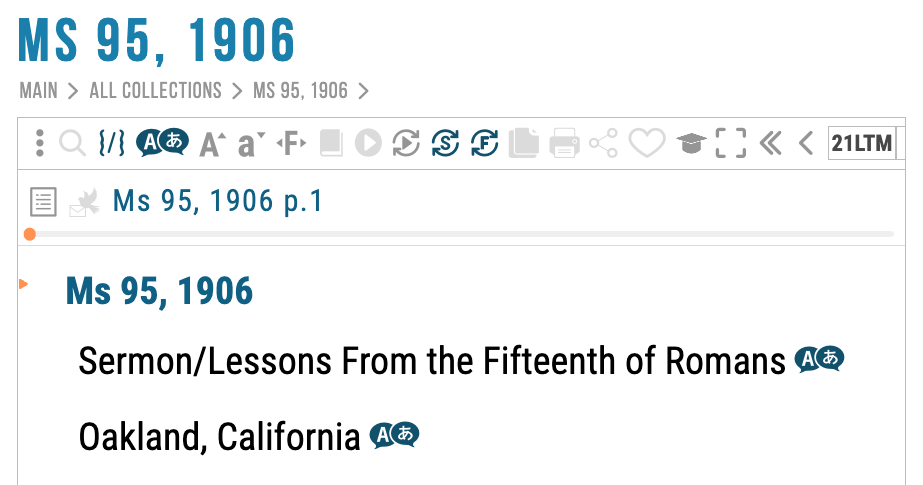
\includegraphics[width=1\linewidth]{images/sermons-and-talks.png}
    \label{fig:enter-label}
\end{figure}

Dla nas osobiście te cytaty są niepotwierdzone i nieważne, zwłaszcza w świetle potwierdzonych dzieł Ellen White. Lecz jeżeli ktoś nalega, aby traktować jej niepotwierdzone sprawozdania na równi z opublikowanymi pismami, nie będziemy się temu sprzeciwiać, ale jeszcze bardziej podkreślimy wniosek o Duchu Świętym jako istocie. Prześledźmy to razem.

Nawet w świetle uwierzytelnionych dzieł Ellen White, taki Duch Święty, istota, nie byłby jedno z Bogiem, ponieważ Chrystus był \egwinline{\textbf{jedyną istotą, która była jedno z Bogiem}}[Lt121-1897.7; 1897][https://egwwritings.org/read?panels=p7266.13]. Ten Duch Święty, istota, nie mógłby \egwinline{\textbf{wejść we wszystkie rady i zamiary Boga}}, ponieważ Chrystus był \egwinline{\textbf{jedyną istotą}}[PP 34.1; 1890][https://egwwritings.org/read?panels=p84.75], która mogła to zrobić. Ta Istota nie ma być wywyższana, ponieważ \egwinline{\textbf{\underline{jedynie} Ojciec i Syn mają być wywyższeni}}[YI, 7 lipca 1898, akap. 2.][https://egwwritings.org/read?panels=p469.2964]. Duch Święty, jako istota, nie pasowałby do porządku nieba jako trzecia istota, ponieważ szatan był \egwinline{\textbf{zaraz po Chrystusie najbardziej wywyższoną \underline{istotą}} na niebiańskich dworach}[RH, 9 sierpnia 1898, akap. 7.][https://egwwritings.org/read?panels=p821.17145]. Ten Duch Święty, istota, nie był zaangażowany w koszt zbawienia; nie był też w przymierzu z Ojcem i Synem, aby zbawić świat, ani nie został znieważony przez występek człowieka.

\egwinline{Wielki dar zbawienia został umieszczony w naszym zasięgu za \textbf{nieskończoną cenę poniesioną przez Ojca i Syna}}[RH, 21 listopada 1912, akap. 2.][https://egwwritings.org/read?panels=p821.33329].

\egwinline{W planie ratowania zgubionego świata rada była między nimi \textbf{\underline{oboma}}; \textbf{przymierze pokoju było między Ojcem a Synem}}[ST, 23 grudnia 1897, akap. 2.][https://egwwritings.org/read?panels=p820.14803].

\egwinline{Ale w przestępstwie człowieka \textbf{\underline{zarówno} Ojciec, jak i Syn zostali znieważeni}.}[ST, 12 grudnia 1895, akap . 7.][https://egwwritings.org/read?panels=p820.13243]

Taki Duch Święty, jako istota, nie jest zgodny z potwierdzonymi relacjami Ellen White ani z Pismem Świętym. Duch Święty jest nazywany ‘\textit{duchem}’, więc jest wyłącznie duchem.

Wiele cytatów siostry White pochodzi z kazań lub przemówień, które zostały opublikowane po jej śmierci. W dalszej części przedstawimy kilka, które są najczęściej omawiane w celu udowodnienia, że siostra White była trynitarianką. Zachęcamy wszystkich do porównania tych cytatów z jej potwierdzonymi i opublikowanymi za jej życia dziełami.

„\textit{I potem są dotykane złote harfy, a muzyka płynie przez wszystkie zastępy niebiańskie, i padają oni, oddając pokłon Ojcu i Synowi, i Duchowi Świętemu}”\footnote{\href{https://egwwritings.org/?ref=en_Ms139-1906.32&para=9579.38}{EGW; Ms139-1906.32; 1906}}. [Kazanie/Rozważania na temat Mt 4. Oakland, Kalifornia, 24 lipca 1906; wcześniej niepublikowane].

„\textit{Musimy zdać sobie sprawę, że Duch Święty, który jest tak samo osobą, jak Bóg jest osobą, przechadza się po tych terenach}”\footnote{\href{https://egwwritings.org/?ref=en_Ms66-1899.11&para=6622.19}{EGW; Ms66-1899.11: 1899}}. [Przemówienie/Fragmenty przemówień wygłoszonych przez panią E. G. White podczas otwarcia College Hall, Avondale, oraz w kościele Avondale].
           % Appendix

% Back matter
\backmatter
\pagestyle{empty}

\cleardoublepage

% Back cover of the book
\begin{center}
\begin{tikzpicture}[remember picture,overlay]
    
    % Black background
    \fill[black] (current page.south west) rectangle (current page.north east);    

    % Central circle pattern
    \begin{scope}[shift={(current page.center)}, scale=1.0871]
        \foreach \x in {-20, -18, -16, -14, -12, -10, -8, -6, -4, -2, 0, 2, 4, 6, 8, 10, 12, 14, 16, 18} {
            \foreach \y in {-2, 2} {
                \begin{scope}[shift={(\x + 1, \y)}]
                    \foreach \r in {0.2, 0.4, 0.6, 0.8, 1.0} {
                        \draw[thick, darkgray] (0,0) circle (\r);
                    }
                \end{scope}
            }
            \foreach \y in {-3, -1, 1, 3} {
                \begin{scope}[shift={(\x, \y)}]
                    \foreach \r in {0.2, 0.4} {
                        \draw[thick, darkgray] (0,0) circle (\r);
                    }
                \end{scope}
            }
            \foreach \y in {-1, 1} {
                \begin{scope}[shift={(\x, 0)}]
                    \foreach \r in {0.2, 0.4, 0.6, 0.8, 1.0} {
                        \draw[thick, lightgray] (0,0) circle (\r);
                    }
                \end{scope}
            }
            \foreach \y in {-1, 1} {
                \begin{scope}[shift={(\x, \y)}]
                    \foreach \r in {0.2, 0.4, 0.6, 0.8, 1.0} {
                        \fill[black] (0,0) circle (\r);
                    }
                \end{scope}
            }
            \foreach \y in {-1, 1} {
                \begin{scope}[shift={(\x, \y)}]
                    \foreach \r in {0.2, 0.4, 0.6, 0.8, 1.0} {
                        \draw[thick, darkgray] (0,0) circle (\r);
                    }
                \end{scope}
            }
        }
    \end{scope}

    % Title
    \node[white, anchor=north, text width =0.9\linewidth, align = justify] at ([yshift=-48pt] current page.north) {\scshape{The Seventh-day Adventist Church is grappling with a persistent doctrinal challenge: the Trinity. While many focus on resolving the doctrine itself, the author argues that the real issue is a deeper character problem. The widespread antagonism between pro- and anti-Trinitarians fuels division. The author proposes a simple step toward constructive dialogue: finding Common Ground. Michael, co-founder of the Forgotten Pillar Project, aims to revive the crucial doctrine on the personality of God, offering a fresh perspective that could bridge the divide. Explore the Trinity controversy through this unique lens and discover the clarity that could bring unity to the church.}};

    % Publisher logo
    \node[anchor=north, above=4pt of publisher.north] {
\includegraphics[width=0.21\textwidth]{images/logo-white.png}};

\end{tikzpicture}
\end{center}
       % Back page (back cover)

\ifepub
\else
  % add two empty pages
  \newpage
  \thispagestyle{empty}
  \mbox{}
  \newpage
  \thispagestyle{empty}
  \mbox{}

  % add full page image from cover based on current language and layout
  \begin{tikzpicture}[remember picture,overlay]
    \node[inner sep=0pt] at (current page.center) {%
      
\includegraphics[width=\paperwidth,height=\paperheight]{lang/\currentlang/covers/\currentlayout/back}%
    };
  \end{tikzpicture}

  % add qrcode at the bottom right corner
  \begin{tikzpicture}[remember picture, overlay]
    \node[anchor=south east, xshift=-0.07\paperwidth, yshift=0.05\paperheight] at (current page.south east) {%
      \textcolor{white}{\qrcode[height=\qrcodesize]{https://forgottenpillar.com/book/the-forgotten-pillar?lang=\currentlang&format=\currentlayout}}%
    };
  \end{tikzpicture}
\fi
\end{document}